%% Bookheader, Nov 8, 2020; July 18, 2022

\documentclass[11pt]{../Support/ourbook}
%% or for landscape, comment out line above and use this one:
%%\documentclass[landscape,11pt]{ourbook}

%% This will keep space from stretching around display math:

\makeatletter
\renewcommand\normalsize{%
   \@setfontsize\normalsize\@xipt{13.6}%
   \abovedisplayskip 11\p@  \@minus6\p@
   \abovedisplayshortskip \z@ 
   \belowdisplayshortskip 6.5\p@ \@minus3\p@
   \belowdisplayskip \abovedisplayskip
   \let\@listi\@listI}
\makeatother
\normalsize


\begin{document}

\tableofcontents
\graphicspath{{../../Chapters/matter_energy_intro/en_US}}
\chapter{Matter and Energy}

The universe is made of matter and energy. Current models posit that the universe
is approximately 68\% dark energy, 27\% dark matter, and 5\% ordinary matter. 
Everything you can see and touch is part of the small part of the universe made 
of ordinary matter. Most science deals with ordinary matter and its interactions; 
highly trained theoretical physicists are currently debating the nature and 
effects of dark matter and dark energy. 
\begin{wrapfigure}{r}{2.5in}
\noindent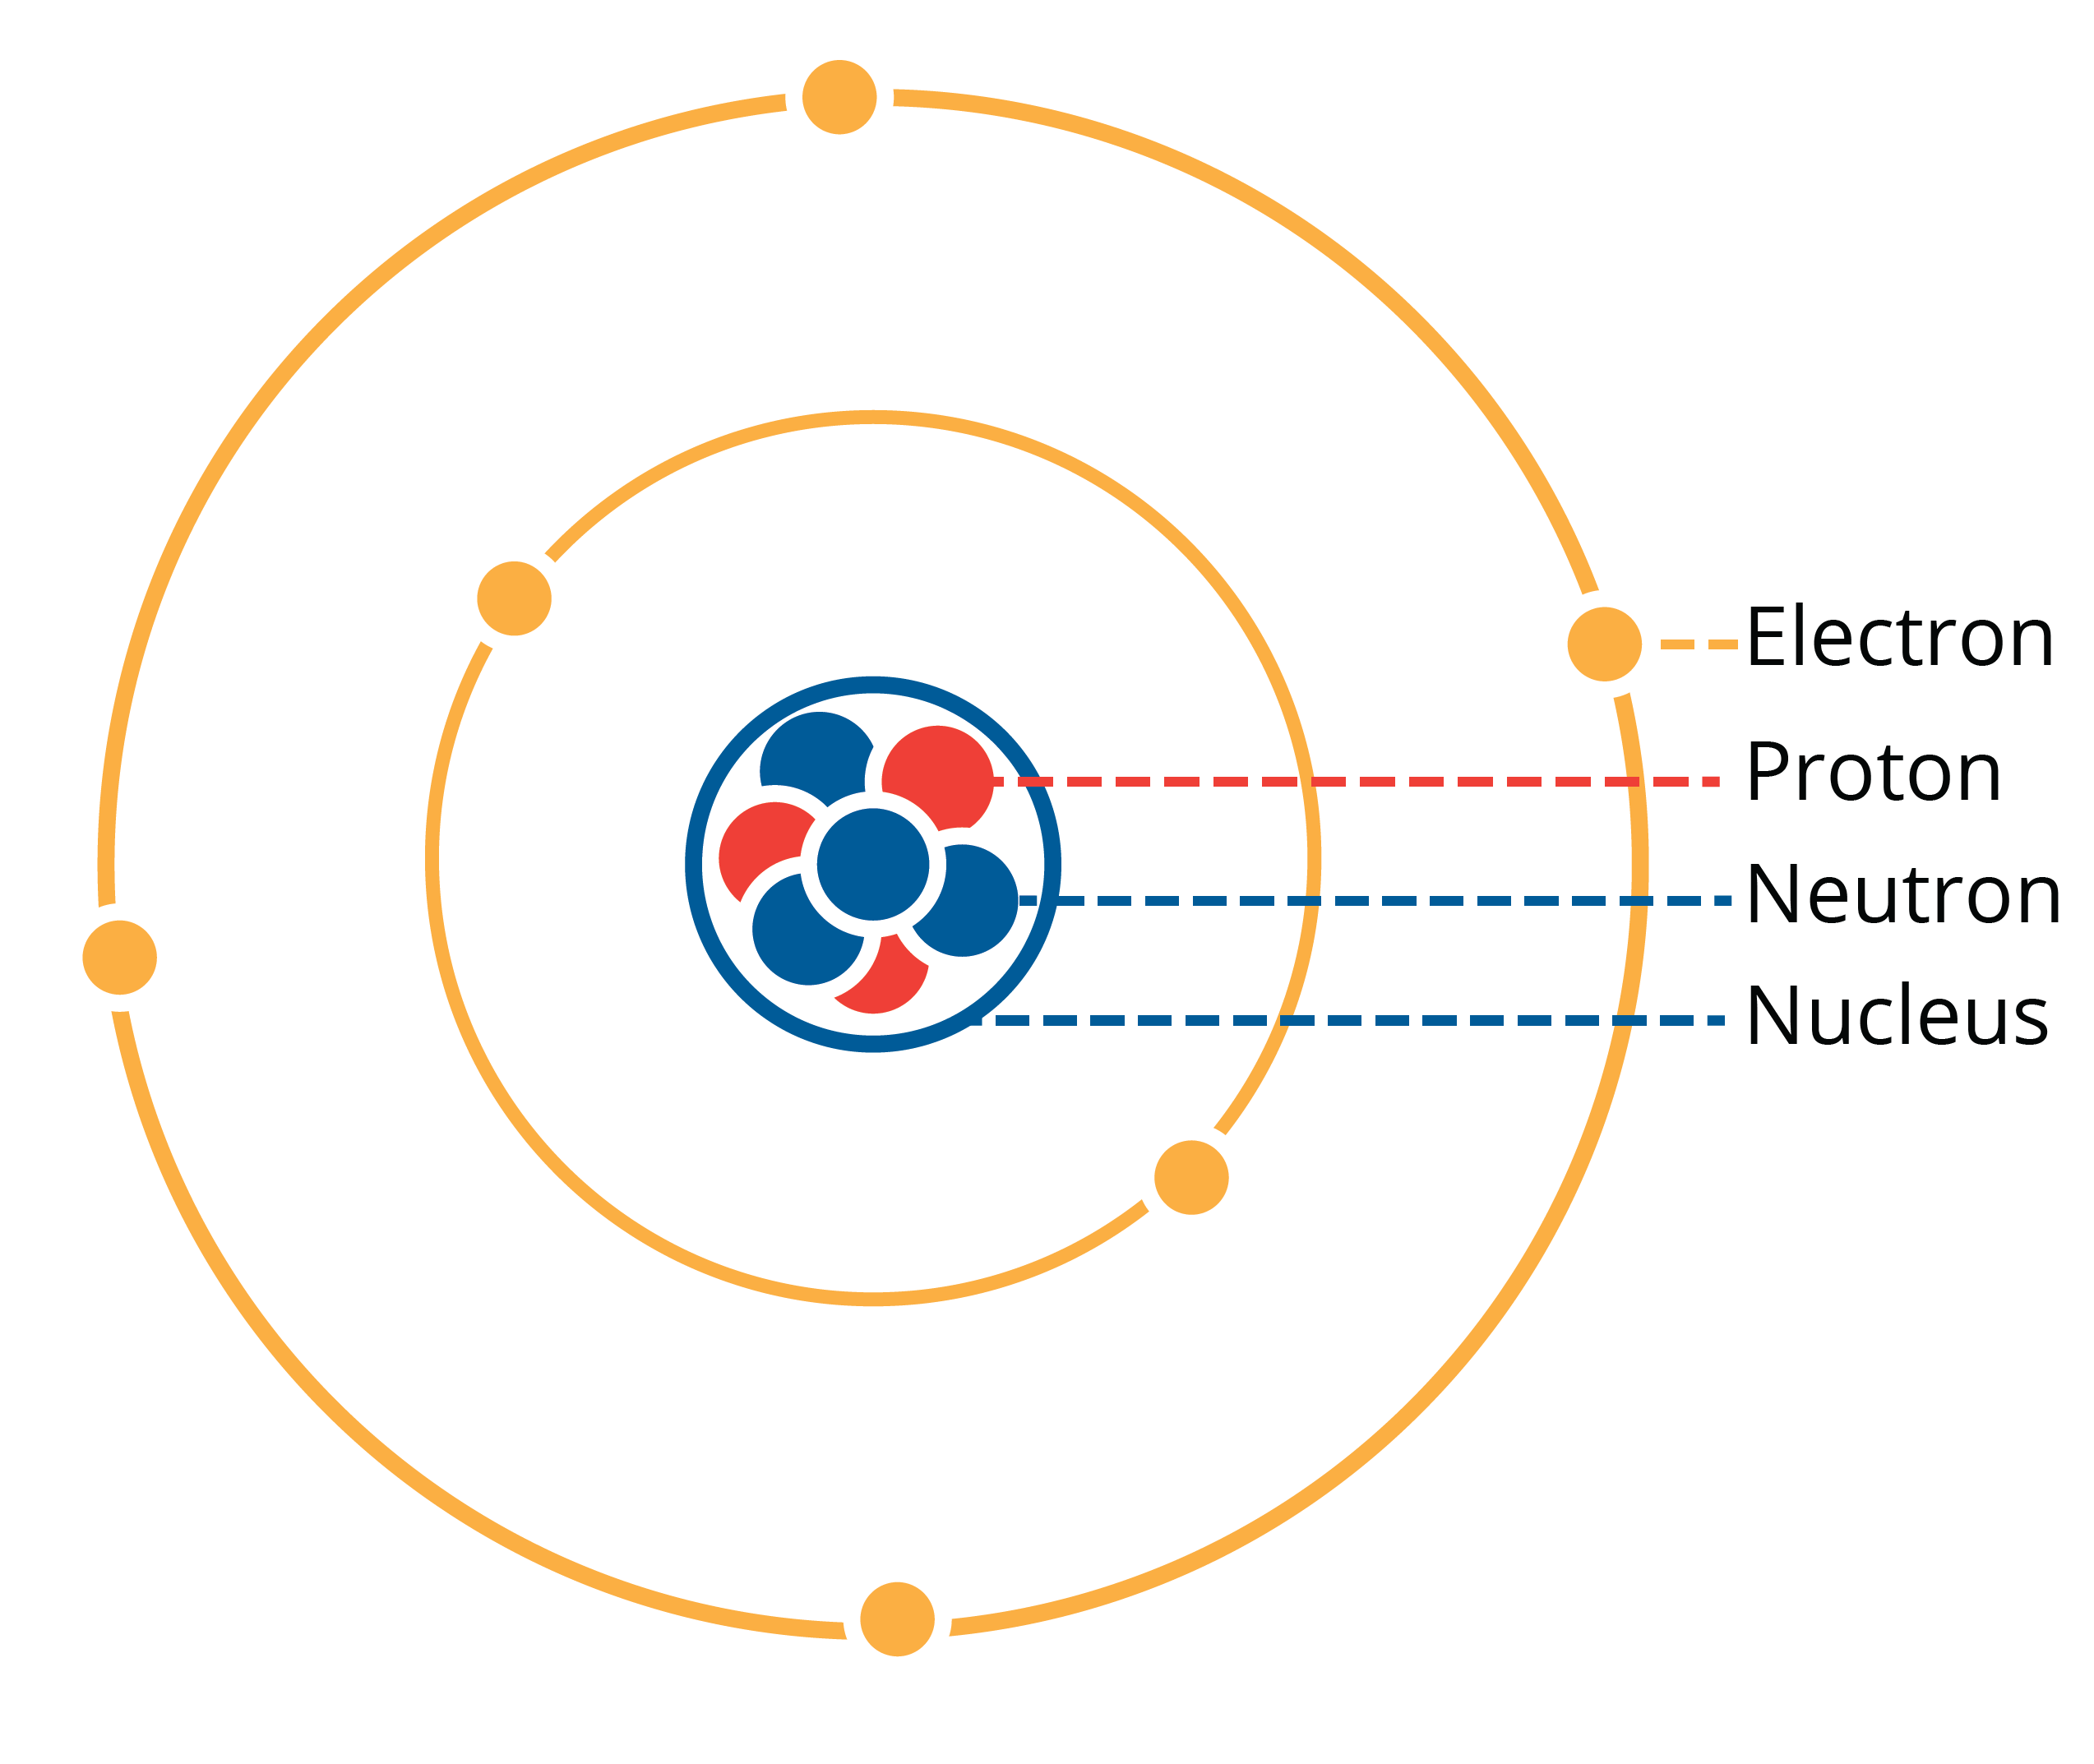
\includegraphics[width=2.5in]{atom1.png}
\caption{}
\label{fig:atom1}
\end{wrapfigure}

What is this ordinary matter made of? All things (including the air around you) 
are made of atoms. Atoms are incredibly tiny --- there are more atoms in a drop 
of water than there are drops of water in all the oceans.
% ADD: If you want a better visual of the scale: https://htwins.net/scale2/, start at around 10^-8

Every atom has a nucleus that contains protons and neutrons. Orbiting around the
nucleus is a cloud of electrons. However, the mass of the atom comes mainly from 
the protons and neutrons, since they are about 2000 times as massive as an 
electron! These three particles, protons, neutrons, and electrons, are called
\textit{subatomic particles}. (See figure \ref{fig:atom1}.) \index{protons} 
\index{neutrons} \index{electrons} \index{subatomic particle}

\section{Atoms and Their Models}
Over the history of science, there have been many ideas about the structure of
atoms. This history is a good example of how science develops: unexpected
results drive scientists to update their models, moving us closer and closer to
a true model of the atom.

During his investigations into the behavior of gases, John Dalton noted that 
different elements combine in strict ratios. For example, he noted that nitrogen 
and oxygen combine in a 1:1 and 1:2 fashion, but no ratio in between.

\begin{wrapfigure}{l}{3in}
\noindent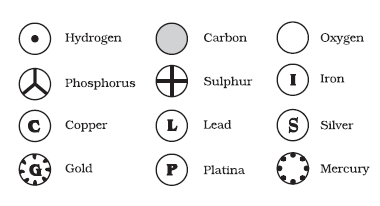
\includegraphics[width=2.5in, trim={0 0.5cm 0 0.5cm}, clip=true]{daltons_model.png}
\caption{Dalton modeled atoms as indivisible and unique.}
\end{wrapfigure}

This first model of the atom is rudimentary; each element is a unique atom,
and those atoms cannot be subdivided. The atom is modeled as one large, solid,
uniform, and neutral object. British physicist J.J. Thomson discovered that
atoms could be split into a light, negatively charged particle and a heavier,
positively charged particle (we now know this is the nucleus, the dense
grouping of protons and neutrons in the center of an atom).

Suddenly, the atom went from neutral and indivisible to made of different types
of charged particles. Further experiments by Ernest Rutherford showed the atom
to be mainly empty space, further updating scientists' model of the atom.
Subsequently, Bohr explained the phenomena of spectral lines (we will discuss
this further in Sequence 2) by modeling electrons as being restricted to
orbiting specific distances from the nucleus.

\begin{wrapfigure}{r}{3in}
\noindent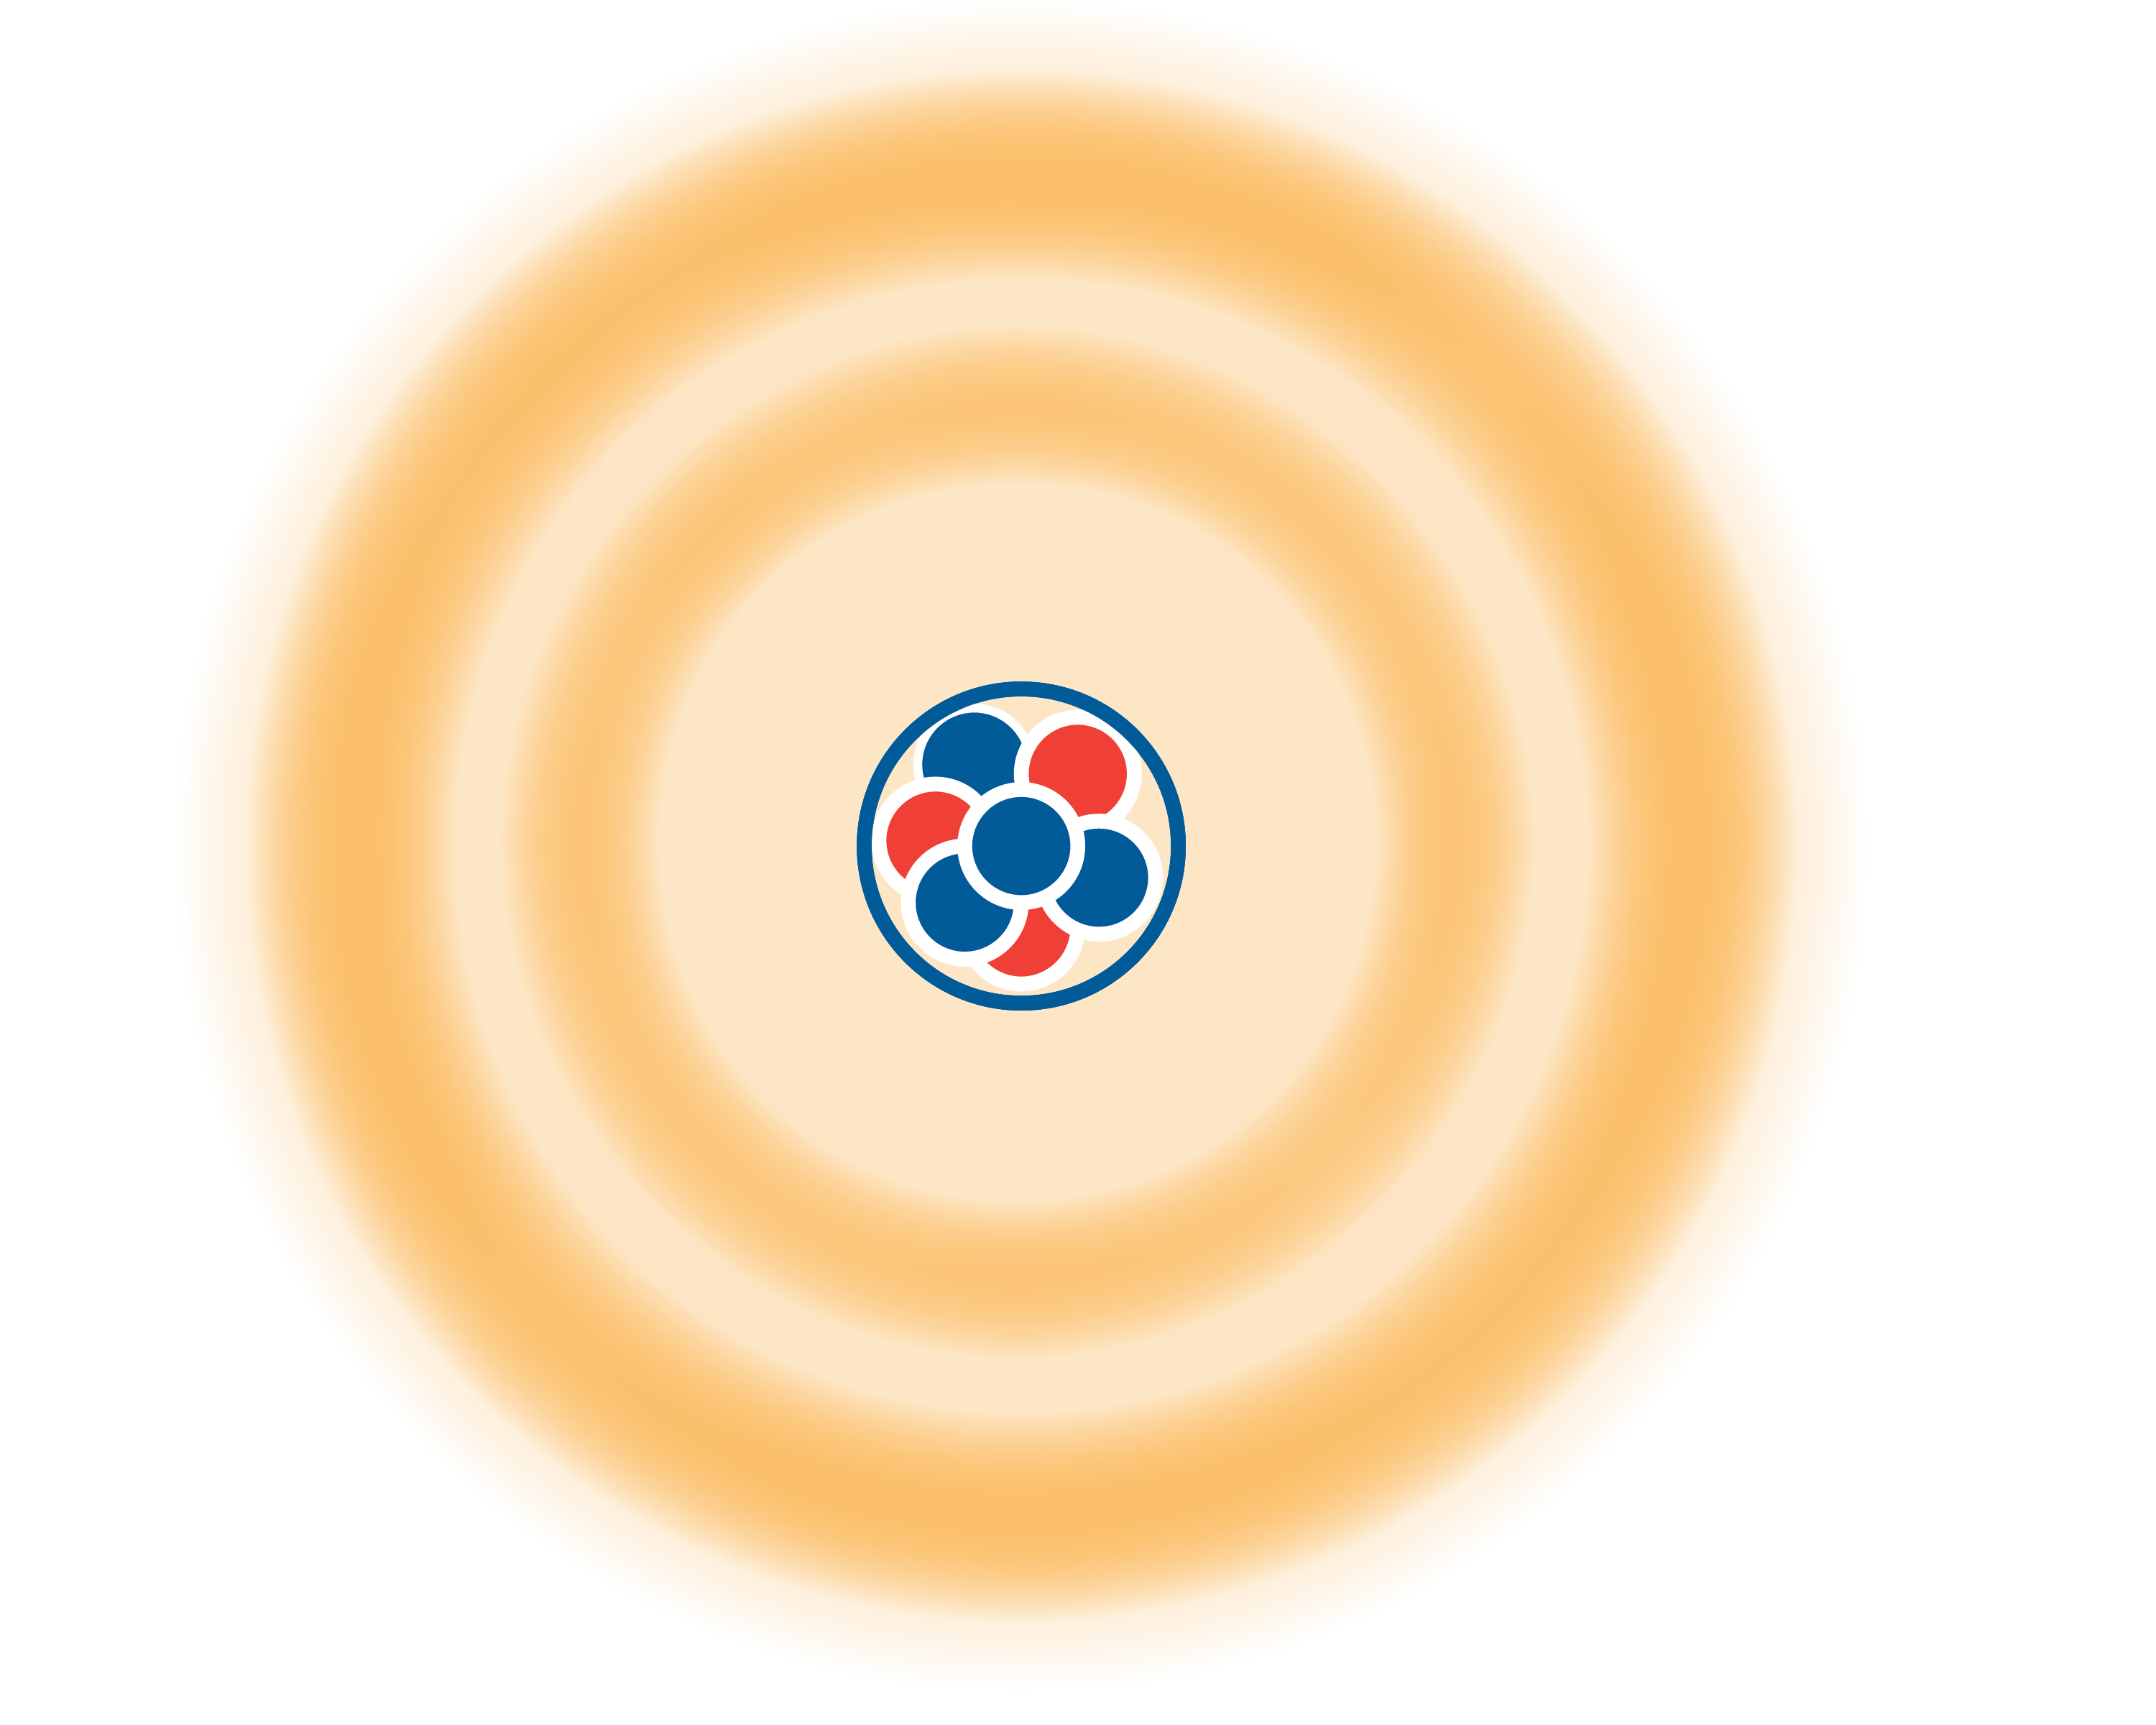
\includegraphics[width=3in]{atomCloud.png}
\caption{}
\label{fig:atomCloud}
\end{wrapfigure}

This is likely the model you are most familiar with seeing, and it is the one we
will use most often in this text. The first figure shown in this chapter is a Bohr
model: it shows the protons and neutrons in the nucleus, and models the electrons 
as moving in discrete orbits around the nucleus. 

However, the Bohr model is slightly inaccurate. While it is a convenient model for
thinking about atoms, in reality, electrons don't neatly orbit the nucleus.
Scientists don't know exactly where an electron will be in relation to the
nucleus, but they do know where it is most likely to be. They use a cloud that is
thicker in the center but fades out at the edges to represent an electron's
position (see figure \ref{fig:atomCloud}).

\begin{wrapfigure}{r}{3in}
\noindent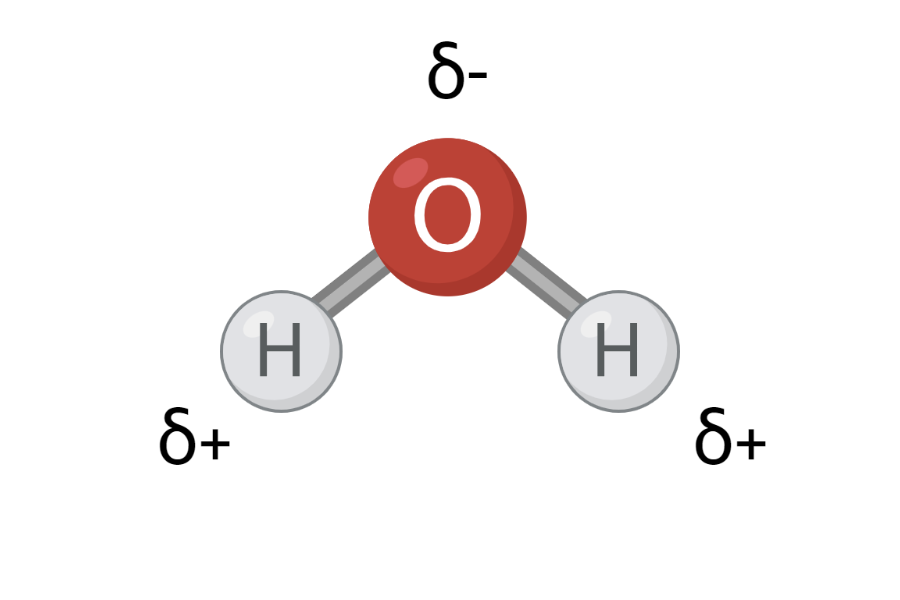
\includegraphics[width=3in]{water_polar.png}
\caption{}
\label{fig:water_polar}
\end{wrapfigure}

While the cloud model is more accurate, we will use the Bohr model as it
allows the viewer to easily and quickly assess the number and arrangement of
electrons.

\subsection{Classifying Atoms}

We classify atoms by the numbers of protons they have. An atom with one proton
is a hydrogen atom, an atom with two protons is a helium atom, and so forth
(refer to periodic table on pg..). We say that hydrogen and helium are \textit{
elements} because the classification of elements is based on the proton number.
And we give each element an atomic symbol. Hydrogen gets $H$, helium gets $He$,
oxygen gets $O$, carbon gets $C$\index{elements}, and so on.

\subsection{When Atoms Combine}
When atoms of different elements combine, they make \textit{compounds}. Compounds
are substances made up of more than one element. Compounds can be 
\textit{molecules} or \textit{crystal lattices}. In the next section you'll learn
\textit{why} these different structures form. 

There are many kinds of compounds. You know a few:
\begin{itemize}
\item Table salt is crystals made of $Na^{+}$ and $Cl^{-}$ ions: a sodium atom 
that as lost an electron and a chlorine atom that gained an electron
\item Baking soda, or sodium bicarbonate, is $NaHCO_3$.
\item $O_2$ is the oxygen molecules that you breathe out of the air (air, a
blend of gases, is mostly $N_2$.).
\item Common quartz is $SiO_2$: silicon dioxide
\end{itemize}

The subscripts indicate what ratio of the elements are present in the compound. 
Each number indicates the ratio for the preceding element. A drop of water, 
$H_2O$, has twice as many hydrogen atoms as oxygen atoms. 

\textbf{Example}: What is the ratio of elements present in Epsom salt?

\textbf{Solution}: Epsom salt, chemical name magnesium sulfate, has the chemical formula $MgSO_4$. Therefore, the ratio of Mg:S:O is 1:1:4. 

%fixme molecule vs formula unit, ordering of bonds versus formulas

\begin{Exercise}[title = {Numbers of Atoms in Molecules}, label = num_atom]
Give the elemental ratio for each compound. 
\begin{enumerate}
\item methane, $CH_4$
\item copper (II) sulfate, $CuSO_4$
\item glucose, $C_6H_{12}O_6$
\end{enumerate}
\end{Exercise}

\begin{Answer}[ref = num_atom]
\begin{enumerate}
\item C:H = 1:4
\item Cu:S:O = 1:1:4
\item C:H:O = 6:12:6 = 1:2:1
\end{enumerate}
\end{Answer}

\section{Types of Matter}
One way to classify matter is by the types of chemical bonds that hold a 
material's atoms together. The nature of these bonds, in turn, affects the 
properties of the material. For now, all you need to know is there are three types
of chemical bonds: metallic, covalent, and ionic. Materials held together with the
same type of bonds tend to have similar properties. For example, copper, bronze, 
iron, and steel (all containing metallic bonds) are all shiny, ductile, malleable,
and good conductors of heat and electricity. On the other hand, Epsom salt and 
table salt for large crystals, have very high melting points, and are poor 
conductors of electricity in their pure form. These two substances (Epsom and 
table salt) both contain ionic bonds. 

\subsection{Ionic Compounds}
Ionic bonds are the electrical attraction between opposite-charged ions. When a 
neutral atom gains or loses an electron it becomes an \textit{ion} (a charged 
atom), and oppositely-charged ions are attracted to each other. Which atom gets 
the electron and which loses it is based on their relative 
\textit{electronegativities}.\index{electronegativity} Electronegativity is simply
a measure of how strongly an atom can attract electrons to itself. In general, 
elements on the right side of the periodic table are more electronegative than 
elements on the left side. There are also polyatomic ions: groups of atoms held 
together with covalent bonds that have an overall charge (figure ... shows a Bohr 
model of a phosphate polyatomic ion, as an example). For now, we'll focus just on 
ionic bonds between monoatomic ions, like in table salt. You'll learn more about 
polyatomic ions and the compounds they form in Sequence 2. 

\begin{wrapfigure}{l}{3in}
\noindent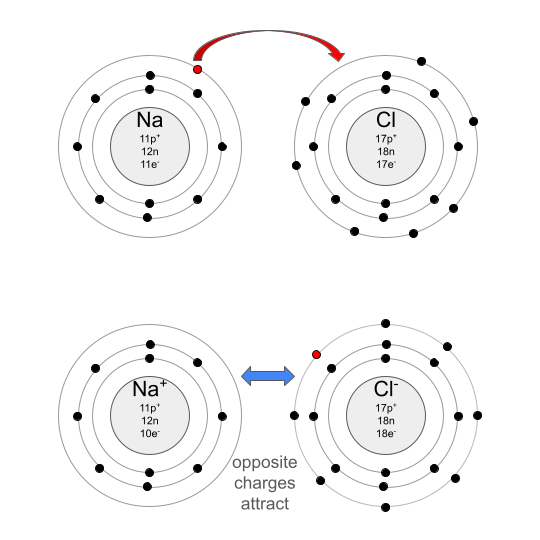
\includegraphics[width=3in]{NaCl_xfer.png}
\caption{}
\label{fig:NaCl_xfer}
\end{wrapfigure}

Let's examine how a simple ionic compound is formed: sodium chloride, also known 
as table salt, is made up of sodium and chlorine atoms (see figure 
\ref{fig:NaCl_xfer}). When sodium and chlorine come in contact with each other, 
electrons move from the sodium to the chlorine, making a sodium \textit{cation} 
(positively-charged ion) and a chloride \textit{anion} (negatively-charged ion). 
Yes --- chlor\textit{ide} is correct! When naming an anion, the ending of the 
element name changes to \textit{-ide}. Once the sodium cation and chloride anion 
are formed, their opposite charges attract them to each other, like north and 
south magnet poles. 

\begin{wrapfigure}{l}{3in}
\noindent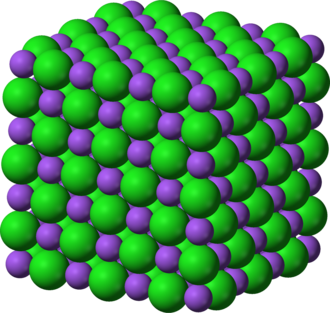
\includegraphics[width=2in]{NaCl_lattice.png}
\caption{}
\label{fig:NaCl_lattice}
\end{wrapfigure}

When there are many, many sodium and chloride ions around, they spontaneously 
arrange themselves in a pattern, giving ionic compounds their characteristic 
crystal structure (see figure \ref{fig:NaCl_lattice}). Because the electrons are 
tightly held be each ion, ionic substances don't conduct electricity well as 
solids. The atomic crystal lattice also determines the shape of the macroscopic 
crystals. Salt crystals are generally cubic, while other crystals (like quartz) 
form hexagonal prisms. You'll learn how to predict the atomic and macroscopic 
crystal structure of different compounds in Sequence 2. 

\subsection{Covalent Compounds}
Water is an example of a covalent compound: it is made of two hydrogen atoms 
covalently bonded one oxygen atom (see figure \ref{fig:water_polar}). The result 
is a water molecule\index{molecules}. The different atoms cluster together 
because they share electrons in their clouds. This is the nature of a 
\textit{covalent bond}\index{covalent bond}: it is formed when atoms share electrons.
Sometimes, electrons are shared evenly, but in water, they are shared unevenly. 
Due to the difference in electronegativity between hydrogen and oxygen, the 
shared electrons are more attracted to the oxygen atom than the hydrogen atoms, 
so they spend more time on the oxygen atom. As a result, the oxygen side of a 
water molecule has a slight negative charge, while the hydrogen atoms have a 
slight positive charge. The slight charges are represented with a lower case 
Greek letter delta, $\delta$. When electrons are shared unevenly, we call this a
\textit{polar} covalent bond, because there are positive and negative poles at 
either end of the bond. \index{polar bond} \index{non-polar bond}

When covalent bonds form between two elements of similar electronegativities, 
the electrons are shared evenly. We call this a \textit{non-polar} covalent bond. 
Oil is an example of a non-polar covalent substance. Different oils have different
combinations, but all oils are made mainly of carbon and hydrogen, which have similar
electronegativities. For both polar and non-polar covalent bonds, the electrons 
are still held tightly, even if they are shared. Those electrons don't move to 
another molecule: they move around within the molecule they are already a part 
of. Since electrons don't flow freely in covalent substances, they are also poor 
conductors of electricity. But, they generally have lower melting and boiling 
points than ionic compounds. 

What happens when you try to mix oil and water? They don't mix well! This is due 
to the difference between their bond types. Polar substances, like water, mix best
with other polar substances, while non-polar substances, like oils, mix best with 
non-polar substances. You'll learn more about why this is in Sequence 2.

\subsection{Metallic Compounds}
You may already know that metals (both pure and alloyed) are excellent conductors of electricity and heat. This is a consequence of their metallic bonds. 
%fixme complete section, pure vs alloys, free flowing electrons



\section{Energy and Work}

Energy is defined as the ability to do work, but what does this mean? First, we 
need to understand what \textit{work} is. When you lift an object into the air, 
you are doing work on that object. When water turns a turbine in a hydroelectric 
plant, the water is doing work on the turbine. And when you hit the brakes on your
car, the brake pads are doing work on the tires (albeit, negative work). 
\textit{Energy} is being transferred between these pairs of objects when work is 
done. 

Some everyday examples of energy include:
\begin{enumerate}
\item The Calories in your food
\item The light from the Sun
\item Heat in the Earth's mantle
\item The motion of a spinning wheel
\end{enumerate}

Some types of energy are easy to visualize, while others are not. Energy is what 
moves from one object to another when work is being done. When you lift 
something, the energy stored in your body (in the form of sugar and fat) is 
transferred to the object, accelerating it upwards. Your body continues to 
transfer energy as you lift the object against gravity. When you've lifted it as 
high as you can, most of the energy your body lost (we call this "burning 
Calories" colloquially) is stored as \textit{potential energy}, due to the 
object's height. 

Another example is a simple circuit connecting a battery and a light bulb. The 
battery has stored potential energy. When the circuit is complete, the potential 
energy in the battery is transferred to electrons in the light bulb, causing them 
to move and gain kinetic energy. In the light bulb's filament (we are referencing 
old, non-LED light bulbs here!), the electrons encounter resistance, which slows 
them down. The energy the electrons lose in this process is being transformed into 
light and heat, lighting your room. 

%fixme edit/rehome material below



\section{Chemical Reactions}

\begin{wrapfigure}{l}{3in}
\noindent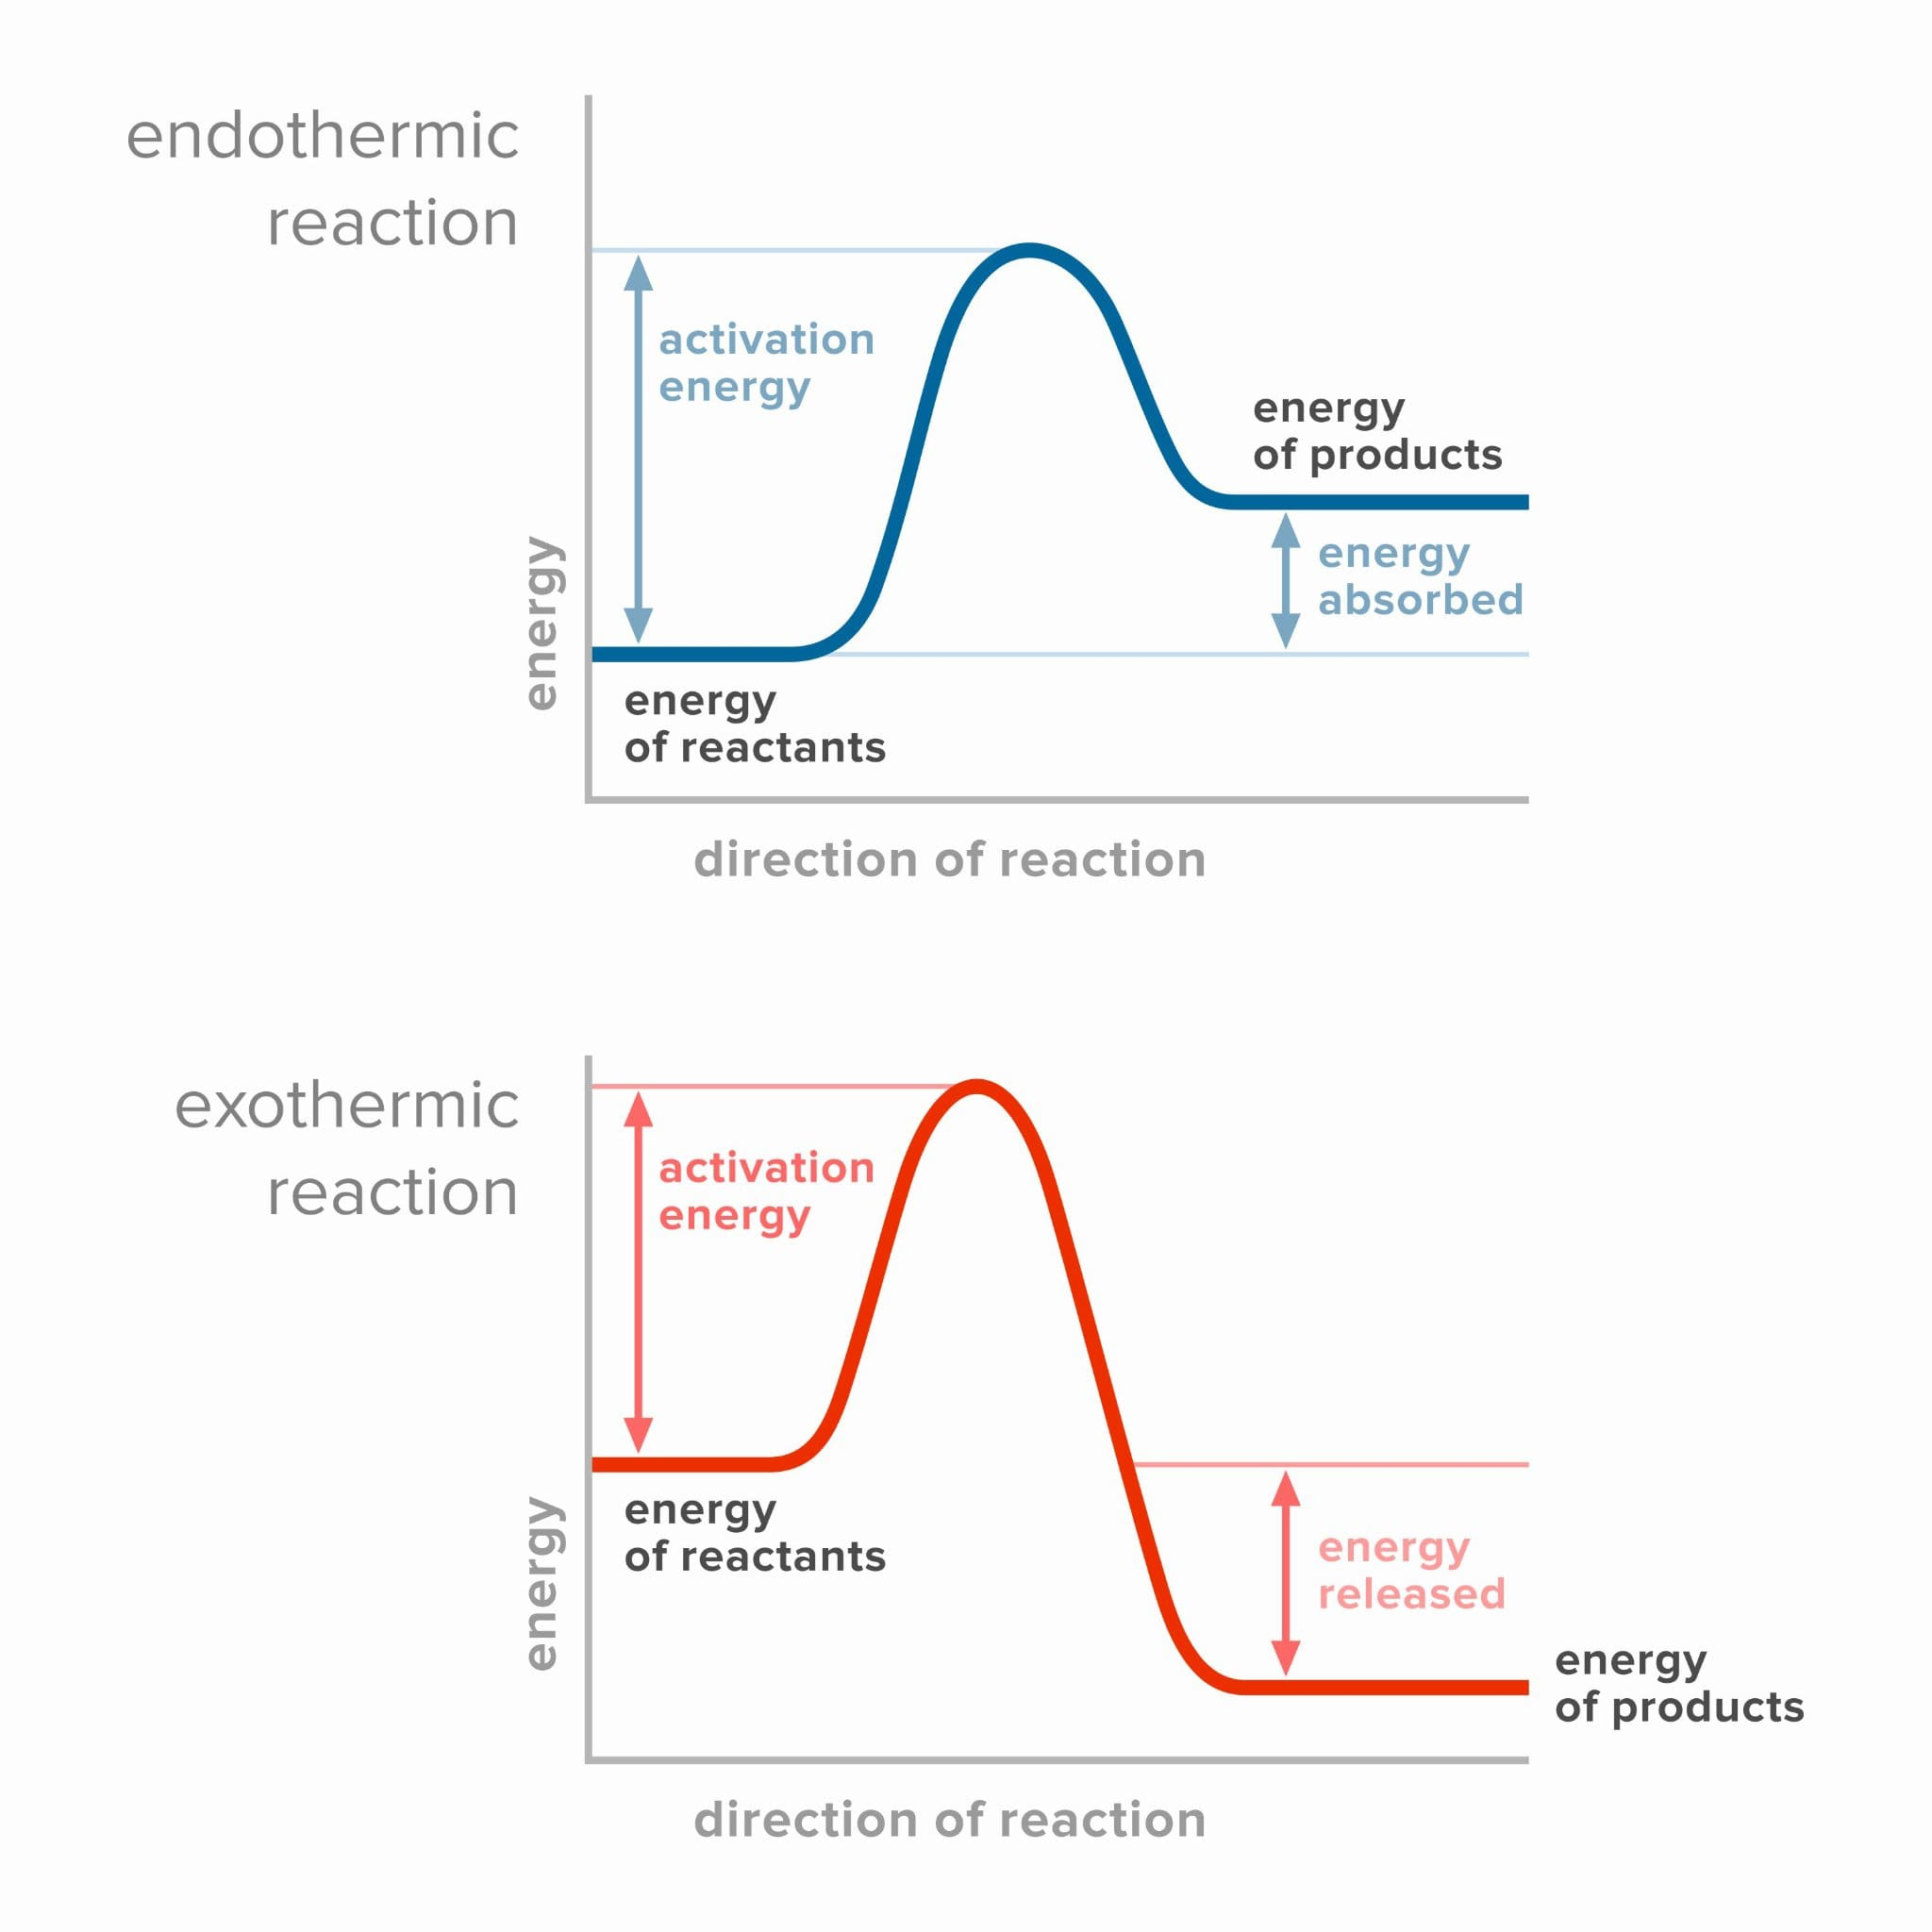
\includegraphics[width=3in]{exo_endo_diagrams.png}
\caption{}
\label{fig:exo_endo_diagrams}
\end{wrapfigure}

Sometimes two hydrogen atoms form a molecule ($H_2$). Sometimes two oxygen
atoms form a molecule ($O_2$). If you mix these together and light a match,
they will rearrange themselves into water molecules. This is called a \textit{
chemical reaction}. In any chemical reaction, the atoms are rearranged into new
molecules.\index{chemical reaction}

Some chemical reactions (like the burning of hydrogen gas described above) are
\textit{exothermic} --- that is, they give off energy. Burning hydrogen gas
happens quickly and gives off a lot of energy. If you have enough, it will make
quite an explosion! \index{exothermic}

Other chemical reactions are \textit{endothermic} --- they consume energy.
Photosynthesis, the process by which plants consume energy from the sun to make
sugar from $CO_2$ and $H_2O$ requires an endothermic chemical reaction.\index{endothermic}

Examine the diagrams in figure \ref{fig:exo_endo_diagrams}. The $x$-axis 
represents time - time passes as wemove from left to right across the diagram. 
At the far left, the energy of the reactants (the ingredients that go into the 
reaction) is shown. At the far right, the energy of the products (what is made in 
the chemical reaction) is shown. The red diagrams shows an exothermic reaction: 
the products (what is made) have less energy than the reactants (the "ingredients"
that start the reaction). Since energy is never created or destroyed, where did 
the energy go? It is released as heat. So, exothermic reactions release heat.

Now, look at the endothermic reaction diagram (the blue one). Based on the
relative energies of the reactants and products, do you expect and endothermic
reaction to release or absorb heat? Absorb! Since the products have more
energy, they must have absorbed energy, in the form of heat, from the surroundings.

What does this look and feel like in real life? If an exothermic reaction were
happening in a glass beaker, you would feel warmth if you held the beaker. The
heat is leaving the beaker and entering your hand, which feels warm. What
about an endothermic reaction? Many students think that since an endothermic
reaction absorbs heat, it must be getting hot. This is incorrect:
\textit{exothermic} reactions feel hot. If an endothermic reaction were
happening in a beaker and you touched the beaker, it would feel \textbf{cold}.
Why? Well, if the reaction is absorbing heat, then heat must be leaving it
surroundings (your hand) and entering the reaction (this heat energy is turned
into chemical energy that is stored in the new chemical bonds that are
forming). So your hand feels cold. %fixme: models showing flow of heat in/out of system for chemical reactions.

\section{Mass and Acceleration}

Each atom has a mass, which means everything made up of those atoms has mass as 
well (and that's pretty much everything!). We measure mass in grams. A paper clip 
is about 1 gram of steel. An adult human can have a mass of 70,000 grams, so for 
larger things, we often talk about kilograms, which is 1000 grams.

The first interesting thing about mass is that objects with more mass
require more force to accelerate. For example, pushing a bicycle so
that it accelerates from a standstill to jogging speed in 2 seconds
requires much less force than pushing a train so that it accelerates
at the same rate.


\begin{mdframed}[style=important, frametitle={Newton's Second Law of Motion}]

The force necessary to accelerate an object of mass $m$ at an acceleration of
$a$ is given by:
$$F = m a$$

This means the force is equal to the mass times the acceleration.

\end{mdframed}

What are the units here? We already know that mass is measured in
kilograms. We can measure velocity in meters per second, but that is
different from acceleration. Acceleration is the rate of change in
velocity. So if we want to go from 0 to 5 meters per second (that's
jogging speed) in two seconds, that is a change in velocity of 2.5
meters per second every second. We would say this acceleration is $2.5
m/s^2$.

\subsection{Calculating Acceleration}
As suggested above, acceleration is a change in velocity. It is calculated by
dividing the change in velocity by the time it takes to make that change.

\begin{mdframed}[style = important, frametitle = {Calculating Acceleration}]
The acceleration of an object from an initial velocity, $v_i$, to a final
velocity, $v_f$, over a period of time, $t$, is given by:

$$a = \frac{v_f - v_i}{t}$$
\end{mdframed}

\textbf{Example}: Your car can go from zero to 60 mph in 3 seconds. What is the
acceleration in $m / s^2$?

\textbf{Solution}: First, let's convert from the imperial units of miles per
hour to the SI units of meters per second. You can do this using a search engine, 
but we will show how to do it by hand below. (You will learn more about this 
method in the Units chapter).

$$\frac{60 \text{ miles}}{1 \text{ hour}} \cdot \frac{1.61 \text{ km}}{1 
\text{ mile}} \cdot \frac{1000\text{ m}}{1\text{ km}} \cdot \frac{1\text{ hour}}{
3600\text{ seconds}} \approx \frac{26.82\text{ m}}{s}$$

Now we have the starting velocity (0 m/s), the ending velocity (26.82 m/s), and 
the time (3 s), and we can find the acceleration:
$$a = \frac{v_f - v_i}{t} = \frac{26.82\frac{m}{s} - 0\frac{m}{s}}{3s} \approx 
8.94 \frac{m}{s^2}$$

\subsection{Determining Force}
What about measuring force? Newton decided to name the unit after himself: The
force necessary to accelerate one kilogram at $1 m/s^2$ is known as \textit{a
newton}. It is often denoted by the symbol $N$.

$$1 N = 1 \frac{kg \cdot m}{s^2}$$

\textbf{Example}: If the car in the above example has a mass of 1500 kg, how much 
force does the engine use to accelerate the car?

\textbf{Solution}: We have already found the car's acceleration: 8.94 $m/s^2$. 
With the mass and acceleration, we can use Newton's Second Law to find the force 
needed to accelerate the car:
$$F = m \cdot a = 1500\text{ kg} \cdot 8.94 \frac{m}{s^2} = 13410\text{ N}$$

\begin{Exercise}[title={Acceleration}, label=acceleration_train]

While driving a bulldozer, you come across a train car (with no brakes
and no locomotive) sitting on a track in the middle of a city. The train car
has a label telling you that it has a mass of 2,400 kg. There is a time-bomb
welded to the interior of the train car, and the timer tells you that
you can safely push the train car for 120 seconds. To get the train
car to where it can explode safely, you need to accelerate it to 20 meters per
second. Fortunately, the track is level and the train car's wheels have
almost no rolling resistance.

With what force, in newtons, do you need to push the train for those 120 seconds?

\end{Exercise}
\begin{Answer}[ref=acceleration_train]
If you accelerate to 20 m/s in 120 s, the acceleration is:
$$a = \frac{v_f - v_i}{t} = \frac{20\text{ m/s} - 0\text{ m/s}}{120\text{ s}} = 
\frac{1}{6} \frac{m}{s^2}$$

To achieve this acceleration, you will need to apply a force of:
$$F = m \cdot a = 2400\text{ kg} \cdot \frac{1}{6} \frac{m}{s^2} = 400\text{ }N$$
\end{Answer}



%FIXME Global layout note: Let's discuss adding Title's and Captions to all graphics.\\

%For example:\\
%TITLE: Mass versus Weight\\
%CAPTION: Human Earth weight: 150lbs / Moon weight:??lbs\\
%Potato Earth weight: .25lbs / Moon weight: ??lbs \\

%FIXME:
%Allison thinks it would be funny if the person in the graphic were holding a potato and we also added the weight and mass of the potato to the caption. No worries if this type of edit isn't in the budget!

%FIXME: What are your thoughts about using the metric system consistently -- in which case we'll replace pounds here with kilos. Max notes: we should explicitly use kilos for mass and pounds or newtons for weight. Kilos are a scalar measure of the amount of matter and pounds are a vector force of gravity on a particular piece of matter. Many students struggle to differentiate between mass and weight at a theoretical level due to casual comparison between pounds and kilos.

\graphicspath{{../../Chapters/atomic_mass/en_US}}
\chapter{Atomic and Molecular Mass}

%fixme add hook

\section{Reading a Periodic Tile}

Let's look at the different information shown on a periodic tile:

\begin{center}
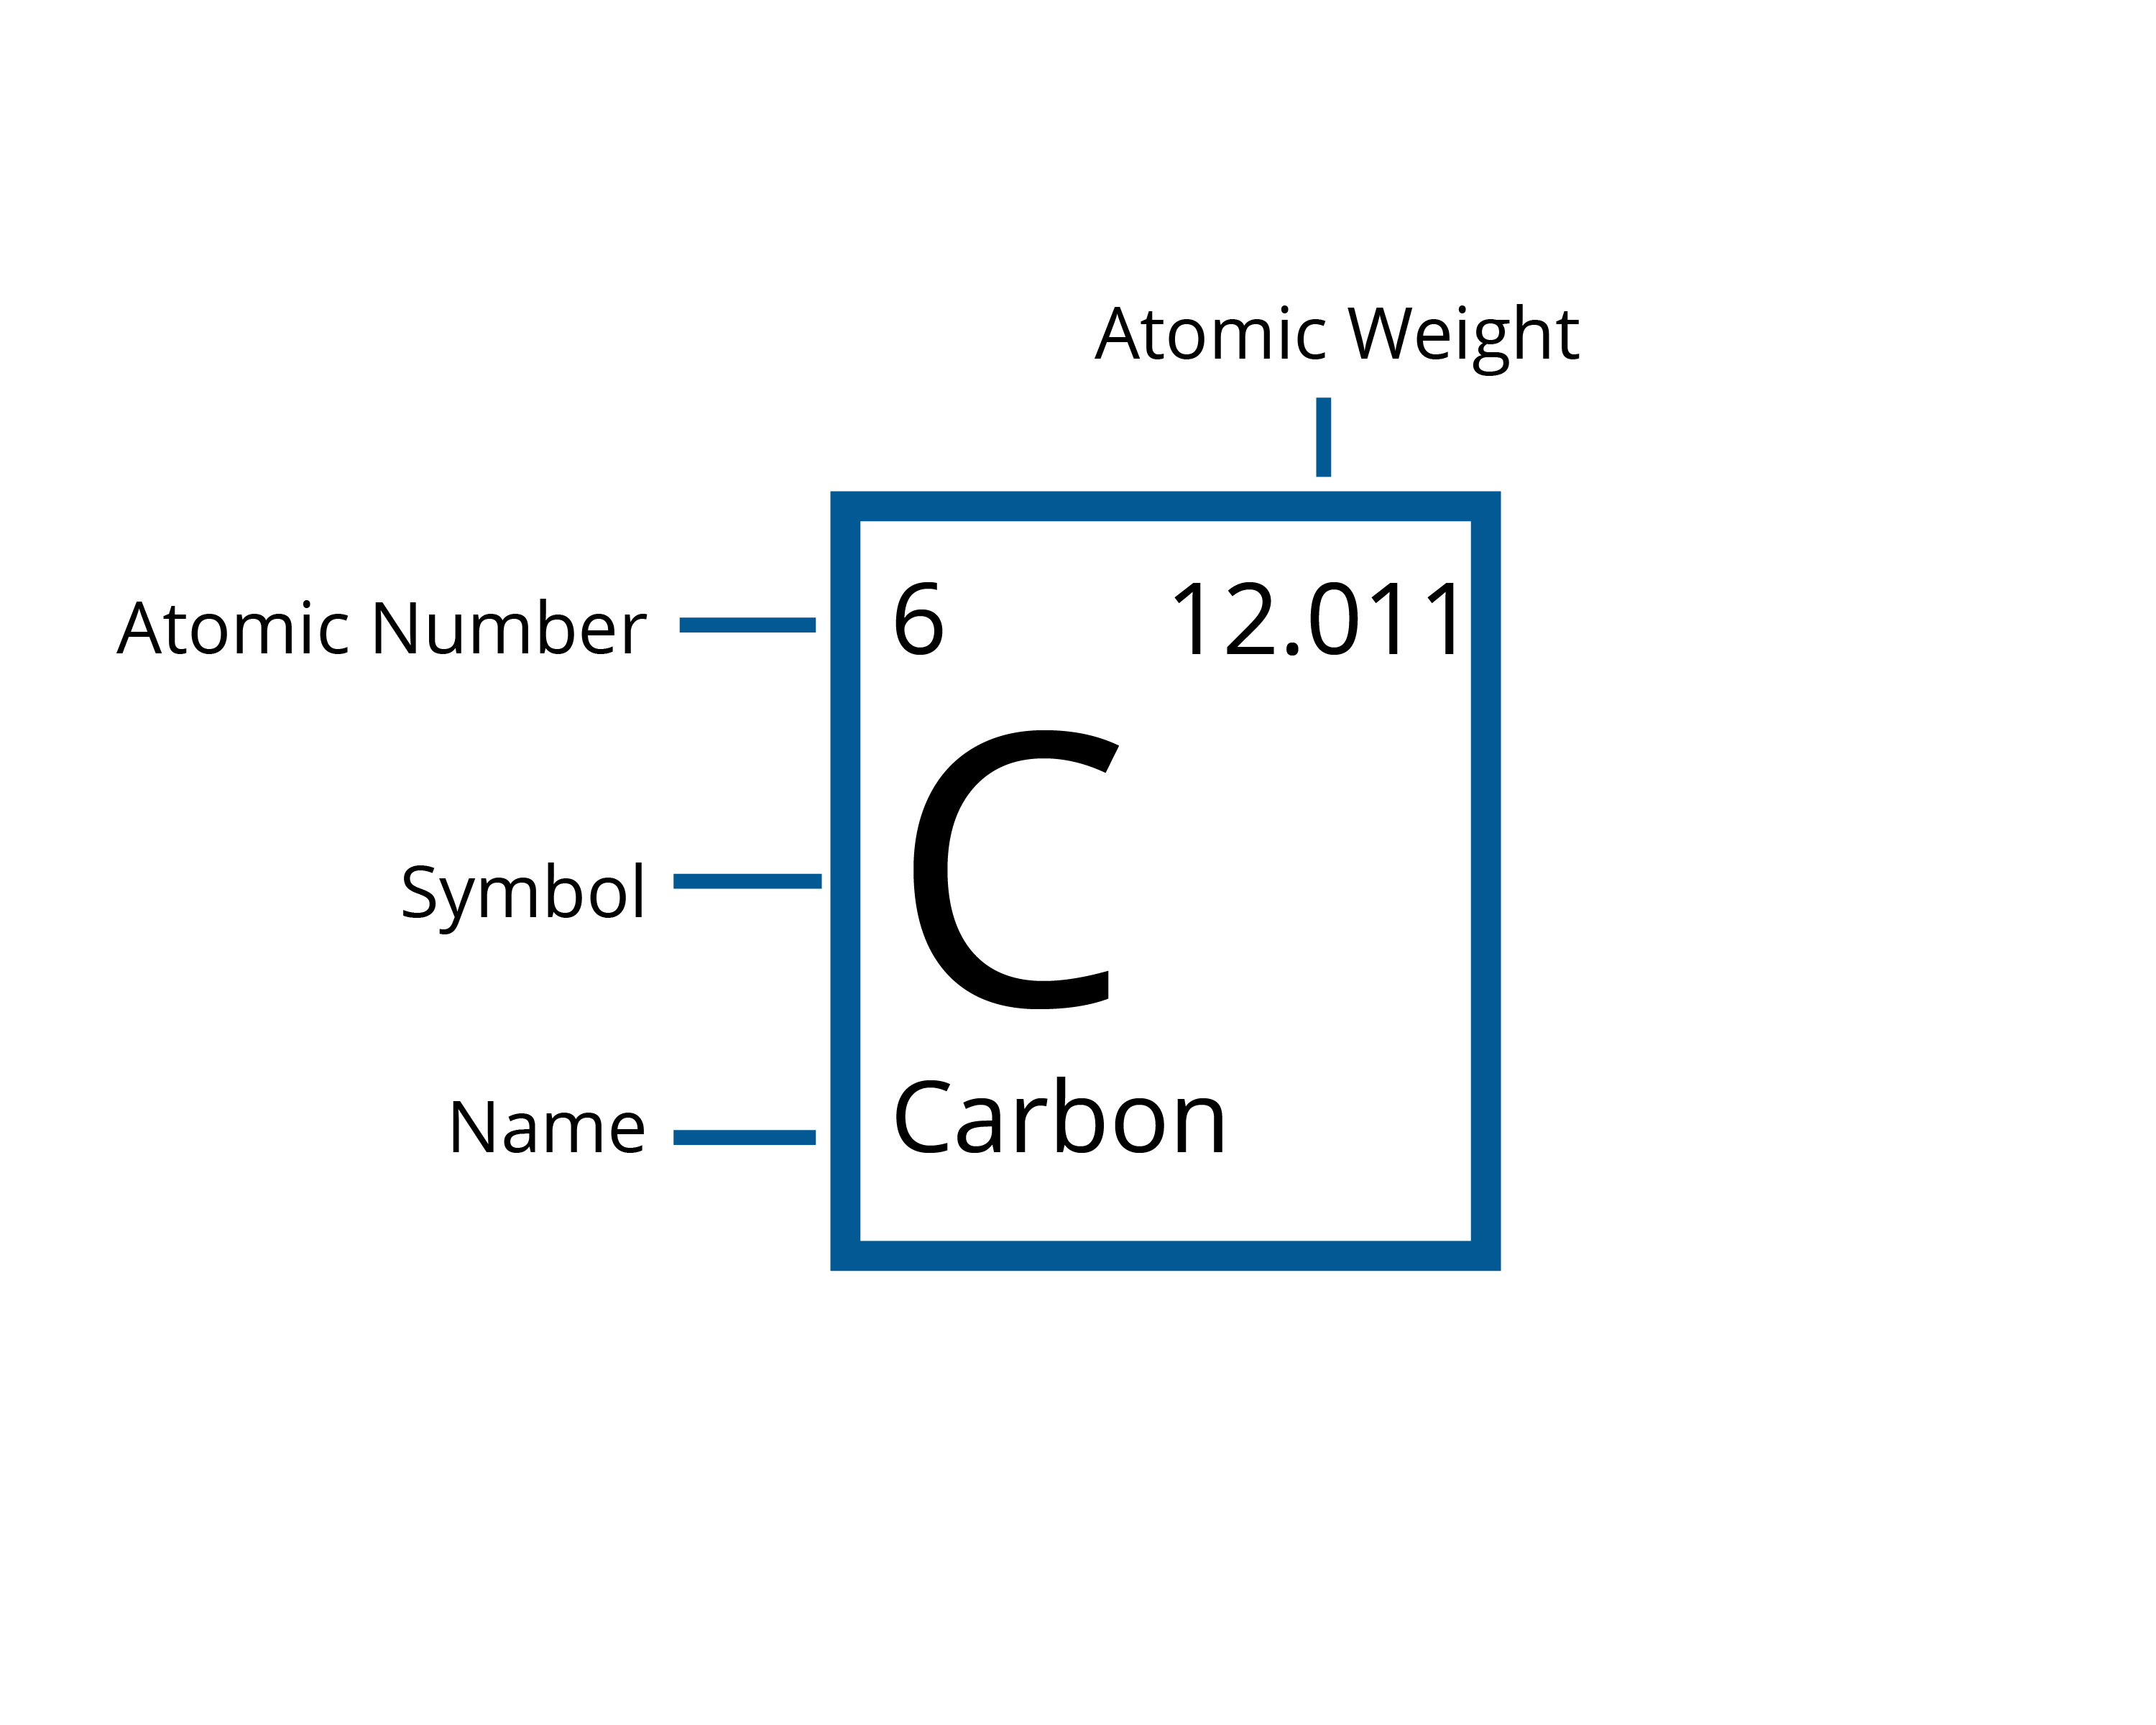
\includegraphics[width = 4in]{element.png}
%fixme change "weight" to "mass" or remake image
\end{center}

The four things we learn from a periodic tile are:
\begin{enumerate}
\item the symbol: as discussed in the previous chapter, each element has a 
unique symbol. Element symbols are used when showing the structure of a molecule
and modeling chemical reactions. 
\item the atomic number: this is also unique for each element. Take a look at the
periodic table a few pages forward. Every tile has a unique atomic number, and 
the tiles are laid out in a generally increasing atomic number (you'll learn why
the periodic table is arranged this way in Sequence 2). 
\item the atomic weight: this is the average mass of all the atoms of that element
in existence. Just like your overall grade in a class is the weighted average of
all the individual grades you earned, atomic weight is the weighted average of the
masses of all the individual atoms of that element. This is also sometimes referred to as atomic mass.
\item the name: not all periodic tables show the name of an element on its tile.
This is why it is useful to know the symbols of common elements. 
\end{enumerate}

Recall from the previous chapter that we classify atoms by the number of protons
they have. What this means is that if we want to know what element an atom is, we
have to look at the number of protons. Take a look at the three carbon atoms below
and note what is the same and what is different among them:

\begin{center}
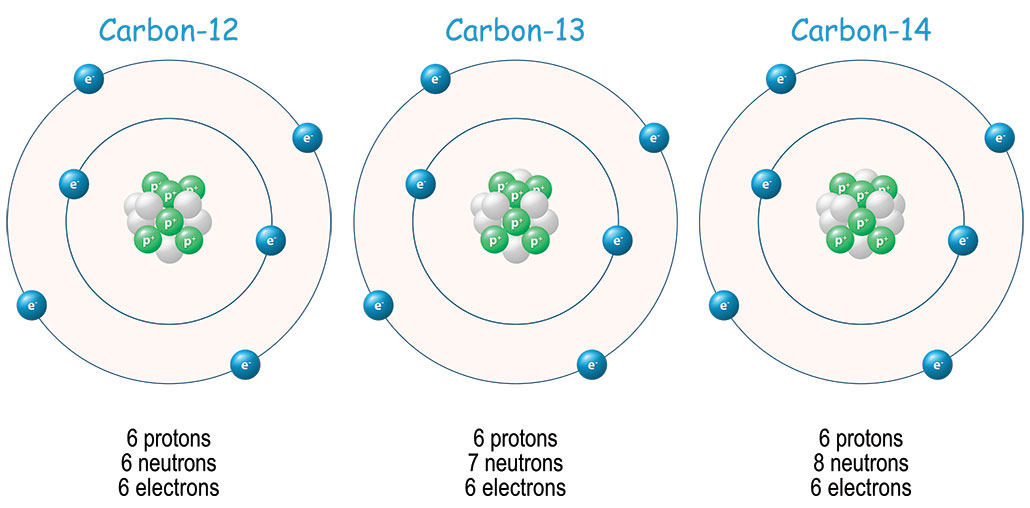
\includegraphics[scale=0.35]{carbon_iso.png}
\end{center}

These different versions of carbon all have 6 protons, which is also carbon's 
atomic number. This isn't a coincidence: the atomic number \textit{is} the number
of protons in every atom of an element. If I tell you an atom has 4 protons, you 
would find atomic number 4 and see that the element is beryllium. To know how many
protons an oxygen atom has, you would find its tile and see that it has atomic 
number 8. 

Ok, so now we know atoms of the same element have the same number of protons, and
that number is given by the element's atomic number. The difference between these
carbon atoms explains the other number on a periodic tile: the atomic mass. 

A proton and a neutron have about the same mass. An electron, on the other hand,
has much less mass: One neutron weighs about the same amount as 2000 electrons. 
This means that the mass of any object comes mostly from the protons and neutrons
in the nucleus of its atoms. \index{proton} \index{neutron}

We know how many protons an atom has by what element it is, but how do we know the 
number of neutrons?

\section{Mass of Atoms and Molecules}
As you've seen, a periodic tile for an element tells us the average mass of an 
atom of that element in Daltons or amus (atomic mass units). The average mass of a
carbon atom is 12.011 amu, and the average mass of an iron atom is 55.845 amu. 
Using the periodic table, determining the average mass of an atom is 
straightforward. What about molecules?

Consider water: $H_2 O$. It is made of 2 hydrogen atoms, each with an average 
mass of 1.008 amu, and one oxygen atom, with an average mass of 15.999 amu. To 
find the mass of the molecule, called \textit{molecular mass}, you simply add the 
masses of each of the atoms in the molecule. So, the molecular mass of water is 
1.008 amu + 1.008 amu + 15.999 amu = 18.015 amu. 

\begin{Exercise}[title = {Determining Molecular Mass}, label = molecular]
Find the molecular mass, in amu, of the following substances:
\begin{enumerate}
\item $CH_4$
\item $CuSO_4$
\item $C_6H_{12}O_6$
\end{enumerate}
\end{Exercise} 

\begin{Answer}[ref = molecular]
\begin{enumerate}
\item 12.011 amu + 4(1.008 amu) = 16.043 amu
\item 63.546 amu + 32.06 amu + 4(15.999 amu) = 159.602 amu
\item 6(12.011 amu) + 12(1.008 amu) + 6(15.999) amu = 180.156 amu
\end{enumerate}
\end{Answer}

\section{Mole Concept}

An atomic mass unit is a very, very, very small unit; we would much rather work in
grams. Grams are a large enough unit that you can develop a natural sense for how 
much a gram is. Additionally, while you can't see a single carbon atom with your 
eyes, you can see 10 grams of carbon (about enough to fill a pen cap). To convert
between the very, very, very small unit of amus to the tangible unit of grams, we 
use \textit{Avogadro's Number} (sometimes called \textit{Avogadro's Constant}).
\index{Avogadro's number}

Since 1 amu is defined as $1/12^{th}$ of the mass of a carbon-12 atom, carbon-12 
by definition has a mass of 12 amu. Additionally, Avogadro's number is the number 
of carbon atoms in 12.000 grams of pure carbon-12. This amount is called \textit{a
mole}. If you have 12 doughnuts, that's a dozen doughnuts. If you have 20 donuts, 
you have a score of donuts. 500 donuts: a ream of donuts. If you have $6.02214076 
\times 10^{23}$ doughnuts, you have a \textit{mole} of doughnuts. This isn't 
really a practical measurement, as a mole of doughnuts would be about the size of 
the earth. We use moles for small things like molecules.\index{mole} However, a mole is a not an abbreviation for a molecule. For a better 
idea about how large of a number Avogadro's number is, you can watch this video: 
\url{https://www.youtube.com/watch?v=TEl4jeETVmg}. 
A mole of carbon-12 has a mass of 12.000 g, but a mole of natural carbon (which
includes all the isotopes of carbon) has a mass of 12.011 g. The mole is defined 
such that one mole of an element is the same mass in grams as one atom is in amus.
Let's say you want to know how much a mole of $NaCl$ weighs. From the periodic 
table, you see that $Na$ has an atomic mass of 22.990 atomic mass units, and $Cl$ 
has 35.453 atomic mass units. One atom of $NaCl$ has a mass of $22.990 + 35.453 = 
58.443$ atomic mass units. This means a mole of $NaCl$ has a mass of $58.443$ 
grams. Handy, right? This is called the \textit{molar mass}. It is the mass of one
mole of a substance, and is given in units of $g/mol$ (grams per mole). The molar 
mass of NaCl is 58.443 g/mol. The molar mass of carbon is 12.011 g/mol. Using 
dimensional analysis and the molar mass, you can determine the mass of a given 
number of moles of a substance. 
% ADD: clarify here that g/mol is numerically equivalent to amus but conceptually different

\textbf{Example}: What is the mass of 2 moles of copper?

\textbf{Solution}: The conversion we will use is 1 mol Cu = 63.546 g Cu.
$$\frac{2 \text{ mol Cu}}{} \times \frac{63.546\text{ g Cu}}{1\text{ mol Cu}} = 
127.092\text{ g Cu}$$

Therefore, 2 moles of copper has a mass of 127.092 grams. 

You can also find the molar mass of a molecule, like methane. Just like with 
elements, a mole of a molecule has the same mass in grams as a single molecule has
in amus. 

\textbf{Example}: What is the mass of 3.5 moles of methane?

\textbf{Solution}: Methane ($CH_4$) has a molecular mass of 16.043 amu, which 
means 1 mole of methane has a mass of 16.043 grams. 

$$\frac{3.5\text{ mol }CH_4}{} \times \frac{16.043{ g }CH_4}{1\text{ mol }CH_4} = 
56.151\text{ g }CH_4$$

You can also use the molar mass to determine how many moles of a substance there 
are in a given mass of that substance.

\textbf{Example}: A standard AAA battery contains about 7.00 g of zinc. How many 
moles of zinc are in a AAA battery?

\textbf{Solution}: Zinc's molar mass is 65.38 g/mol. 
$$\frac{7.00\text{ g Zn}}{} \times \frac{1\text{ mol Zn}}{65.38\text{ g Zn}} 
\approx 0.107\text{ g Zn}$$

In summary, a mole of a substance contains approximately $6.02 \times 10^{23}$ 
particles (atoms or molecules) of that substance and has a mass equal to the 
molecular mass in grams. 

\begin{mdframed}[frametitle = {The Mole Concept}, style = important]
For a substance, X, with a molar mass of $x$ g/mol,
$$1\text{ mol X } = 6.02 \times 10^{23}\text{ particles of X }= x\text{ g of X}$$
\end{mdframed}

\begin{Exercise}[title = {Grams, Moles, Molecules, and Atoms}, label = convert]
Complete the table.

\begin{tabular}{|c|c|c|c|}
\hline
Substance & num. of particles & num. of moles & grams\\\hline
$NaHCO_3$ & & & 35\\\hline
$HCl$ & & 1.2 & \\\hline
$KH_2PO_4$ & $12.5 \times 10^{24}$ & & \\\hline
\end{tabular}
\vspace{75mm}
\end{Exercise}

\begin{Answer}[ref = convert]
\begin{tabular}{|c|c|c|c|}
\hline
Substance & num. of particles & num. of moles & grams \\\hline
$NaHCO_3$ & $2.509 \times 10^{23}$ & 0.4166 & 35.00 \\\hline
$HCl$ & $7.53 \times 10^{23}$ & 1.25 & 45.58 \\\hline
$KH_2PO_4$ & $12.5 \times 10^{24}$ & 20.8 & 2820 \\\hline
\end{tabular}

$$\frac{35.00\text{ g }NaHCO_3}{} \times 
\frac{1\text{ mol } NaHCO_3}{84.007\text{ g }NaHCO_3} = 0.4166\text{ mol }NaHCO_3$$

$$\frac{0.4166\text{ mol }NaHCO_3}{} \times \frac{6.02214076 
\times 10^{23}\text{ molec }NaHCO_3}{1\text{ mol }NaHCO_3} = 
2.509 \times 10^{23}\text{ molec }NaHCO_3$$

$$\frac{1.25\text{ mol }HCl}{} \times 
\frac{36.46\text{ g }HCl}{1\text{ mol }HCl} = 45.58\text{ g }HCl$$

$$\frac{1.25\text{ mol }HCl}{} \times 
\frac{6.02214076 \times 10^{23}\text{ molec }HCl}{1\text{ mol }HCl} 
= 7.53 \times 10^{23}\text{ molec }HCl$$

$$\frac{12.5 \times 10^{24}\text{ molec }KH_2PO_4}{} \times 
\frac{1\text{ mol }KH_2PO_4}{6.02214076 \times 10^{23}\text{ molec }KH_2PO_4} 
= 20.8\text{ mol }KH_2PO_4$$

$$\frac{20.8\text{ mol }KH_2PO_4}{} \times 
\frac{136.086\text{ g }KH_2PO_4}{1\text{ mol }KH_2PO_4} = 
2820\text{ g }KH_2PO_4$$
\end{Answer}

% ADD: Conversions should probably come before this

\begin{Exercise}[title={Burning Methane}, label=burning_methane]

Natural gas is mostly methane ($CH_4$). When one molecule of methane
burns, two oxygen molecules ($O_2$) are consumed. One molecule of
$H_2O$ and one molecule of $CO_2$ are produced.
% ADD: Need to explain mole to mole ratios first, Law of Divine Proportion
% ADD: Include Significant Figures

If you need 200 grams of water, how many grams of methane do you need
to burn?

(This is how the hero in ``The Martian'' made water for his garden.)
\vspace{50mm}
\end{Exercise}

\begin{Answer}[ref=burning_methane]

From the last exercise, you know that 1 mole of water weighs 18.01528
grams, meaning 200 grams of water is about 11.1 moles. So you need to burn
11.1 moles of methane.

What does one mole of methane weigh? Using the periodic table:
$12.0107 + 4 \times 1.00794 = 16.04246$ grams.

$16.0424 \times 11.10 = 178.1$ grams of methane.

\end{Answer}


%final above, pieces below
If you fill a balloon with helium, it will have two different
kinds of helium atoms. Most of the helium atoms will have 2 neutrons, but a
few will have only 1 neutron. We say that these are two different
\textit{isotopes} of helium. We call them helium-4 (or $^4He$) and
helium-3 (or $^3He$). Isotopes are named for the sum of protons and
neutrons the atom has: helium-3 has 2 protons and 1 neutron.\index{isotopes}

A hydrogen atom nearly always has just 1 proton and no neutrons. A
helium atom nearly always has 2 protons and 2 neutrons. So, if you
have a 100 hydrogen atoms and 100 helium atoms, the helium will have
about 4 times more mass than the hydrogen. We say ``Hydrogen is about
1 atomic mass unit (amu), and helium-4 is about 4 atomic mass
units.''\index{atomic mass unit}

What, precisely, is an atomic mass unit? It is defined as 1/12 of
the mass of a carbon-12 atom. Scientists have measured the mass of
helium-4, and it is about 4.0026 atomic mass units. (By the way, an
atomic mass unit is also called a \textit{dalton}.)

\pagebreak


Now you are ready to take a good look at the periodic table of
elements. Here is the version from Wikipedia:\index{periodic table of elements}

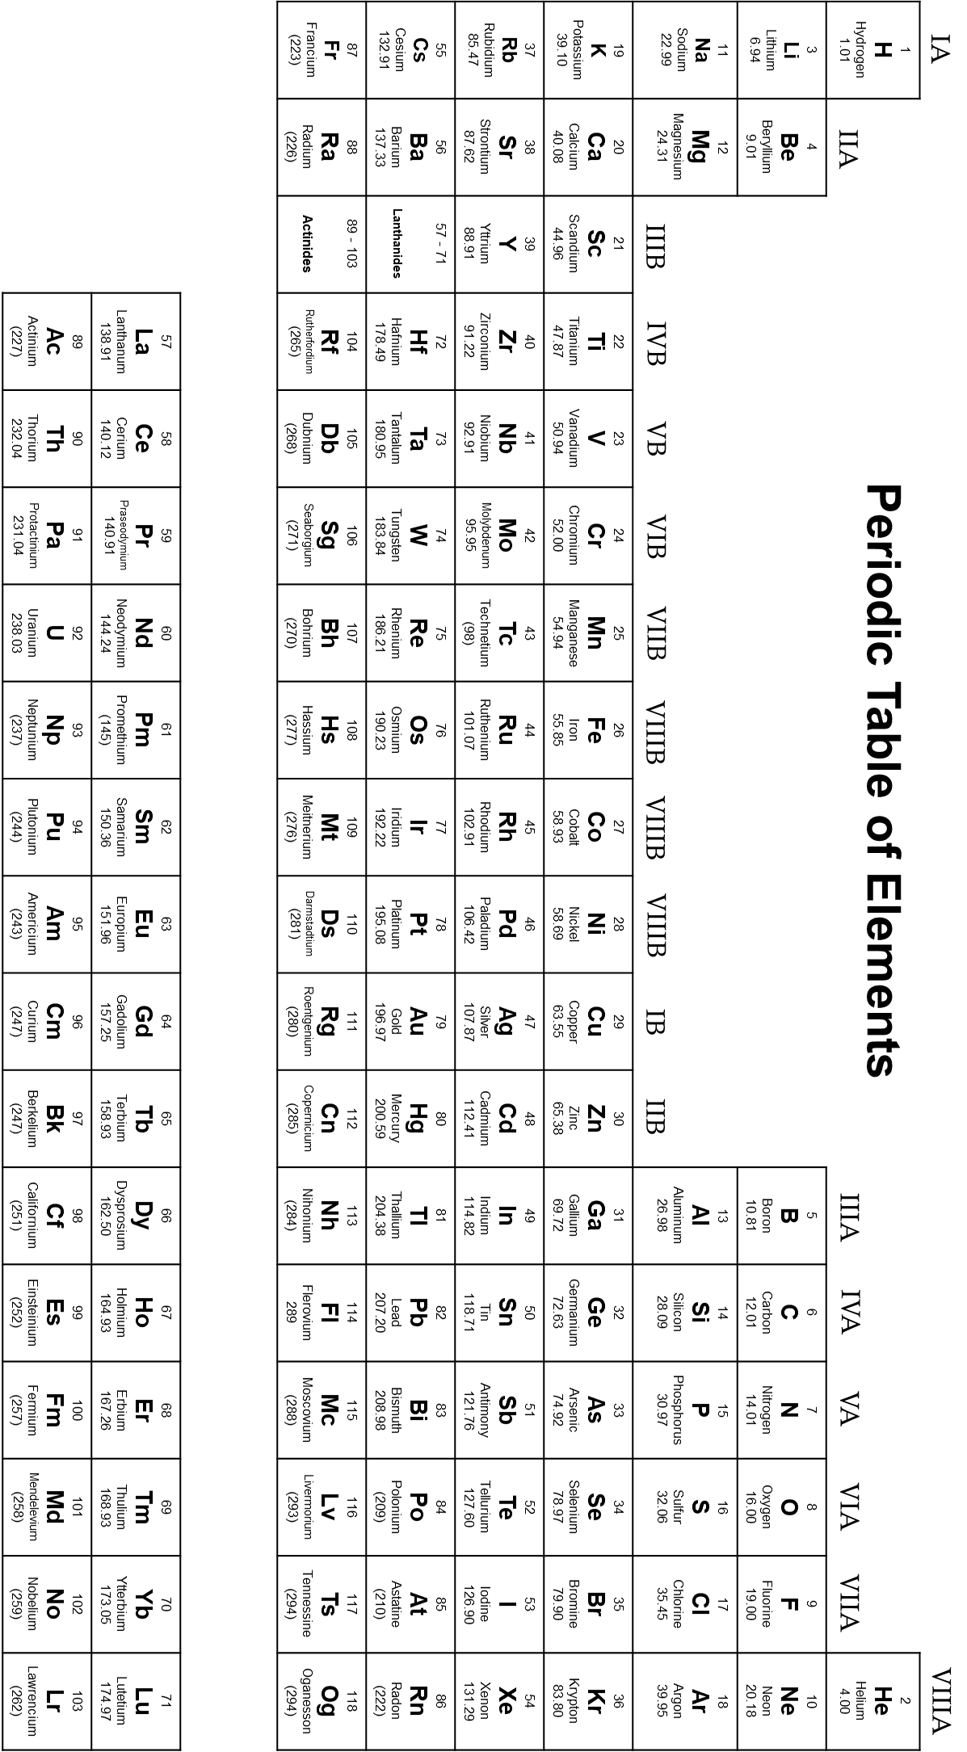
\includegraphics[width=0.75\textwidth]{periodic.png}

% ADD: Periodic Trends, Periods, Collums, Atomic Radius, Electronegativity,

\pagebreak
There is a square for each element. In the middle, you can see the atomic
symbol and the name of the element. In the upper-right corner is the
atomic number --- the number of protons in the atom.

In the upper-left corner is the atomic mass in atomic mass units.\index{atomic mass}

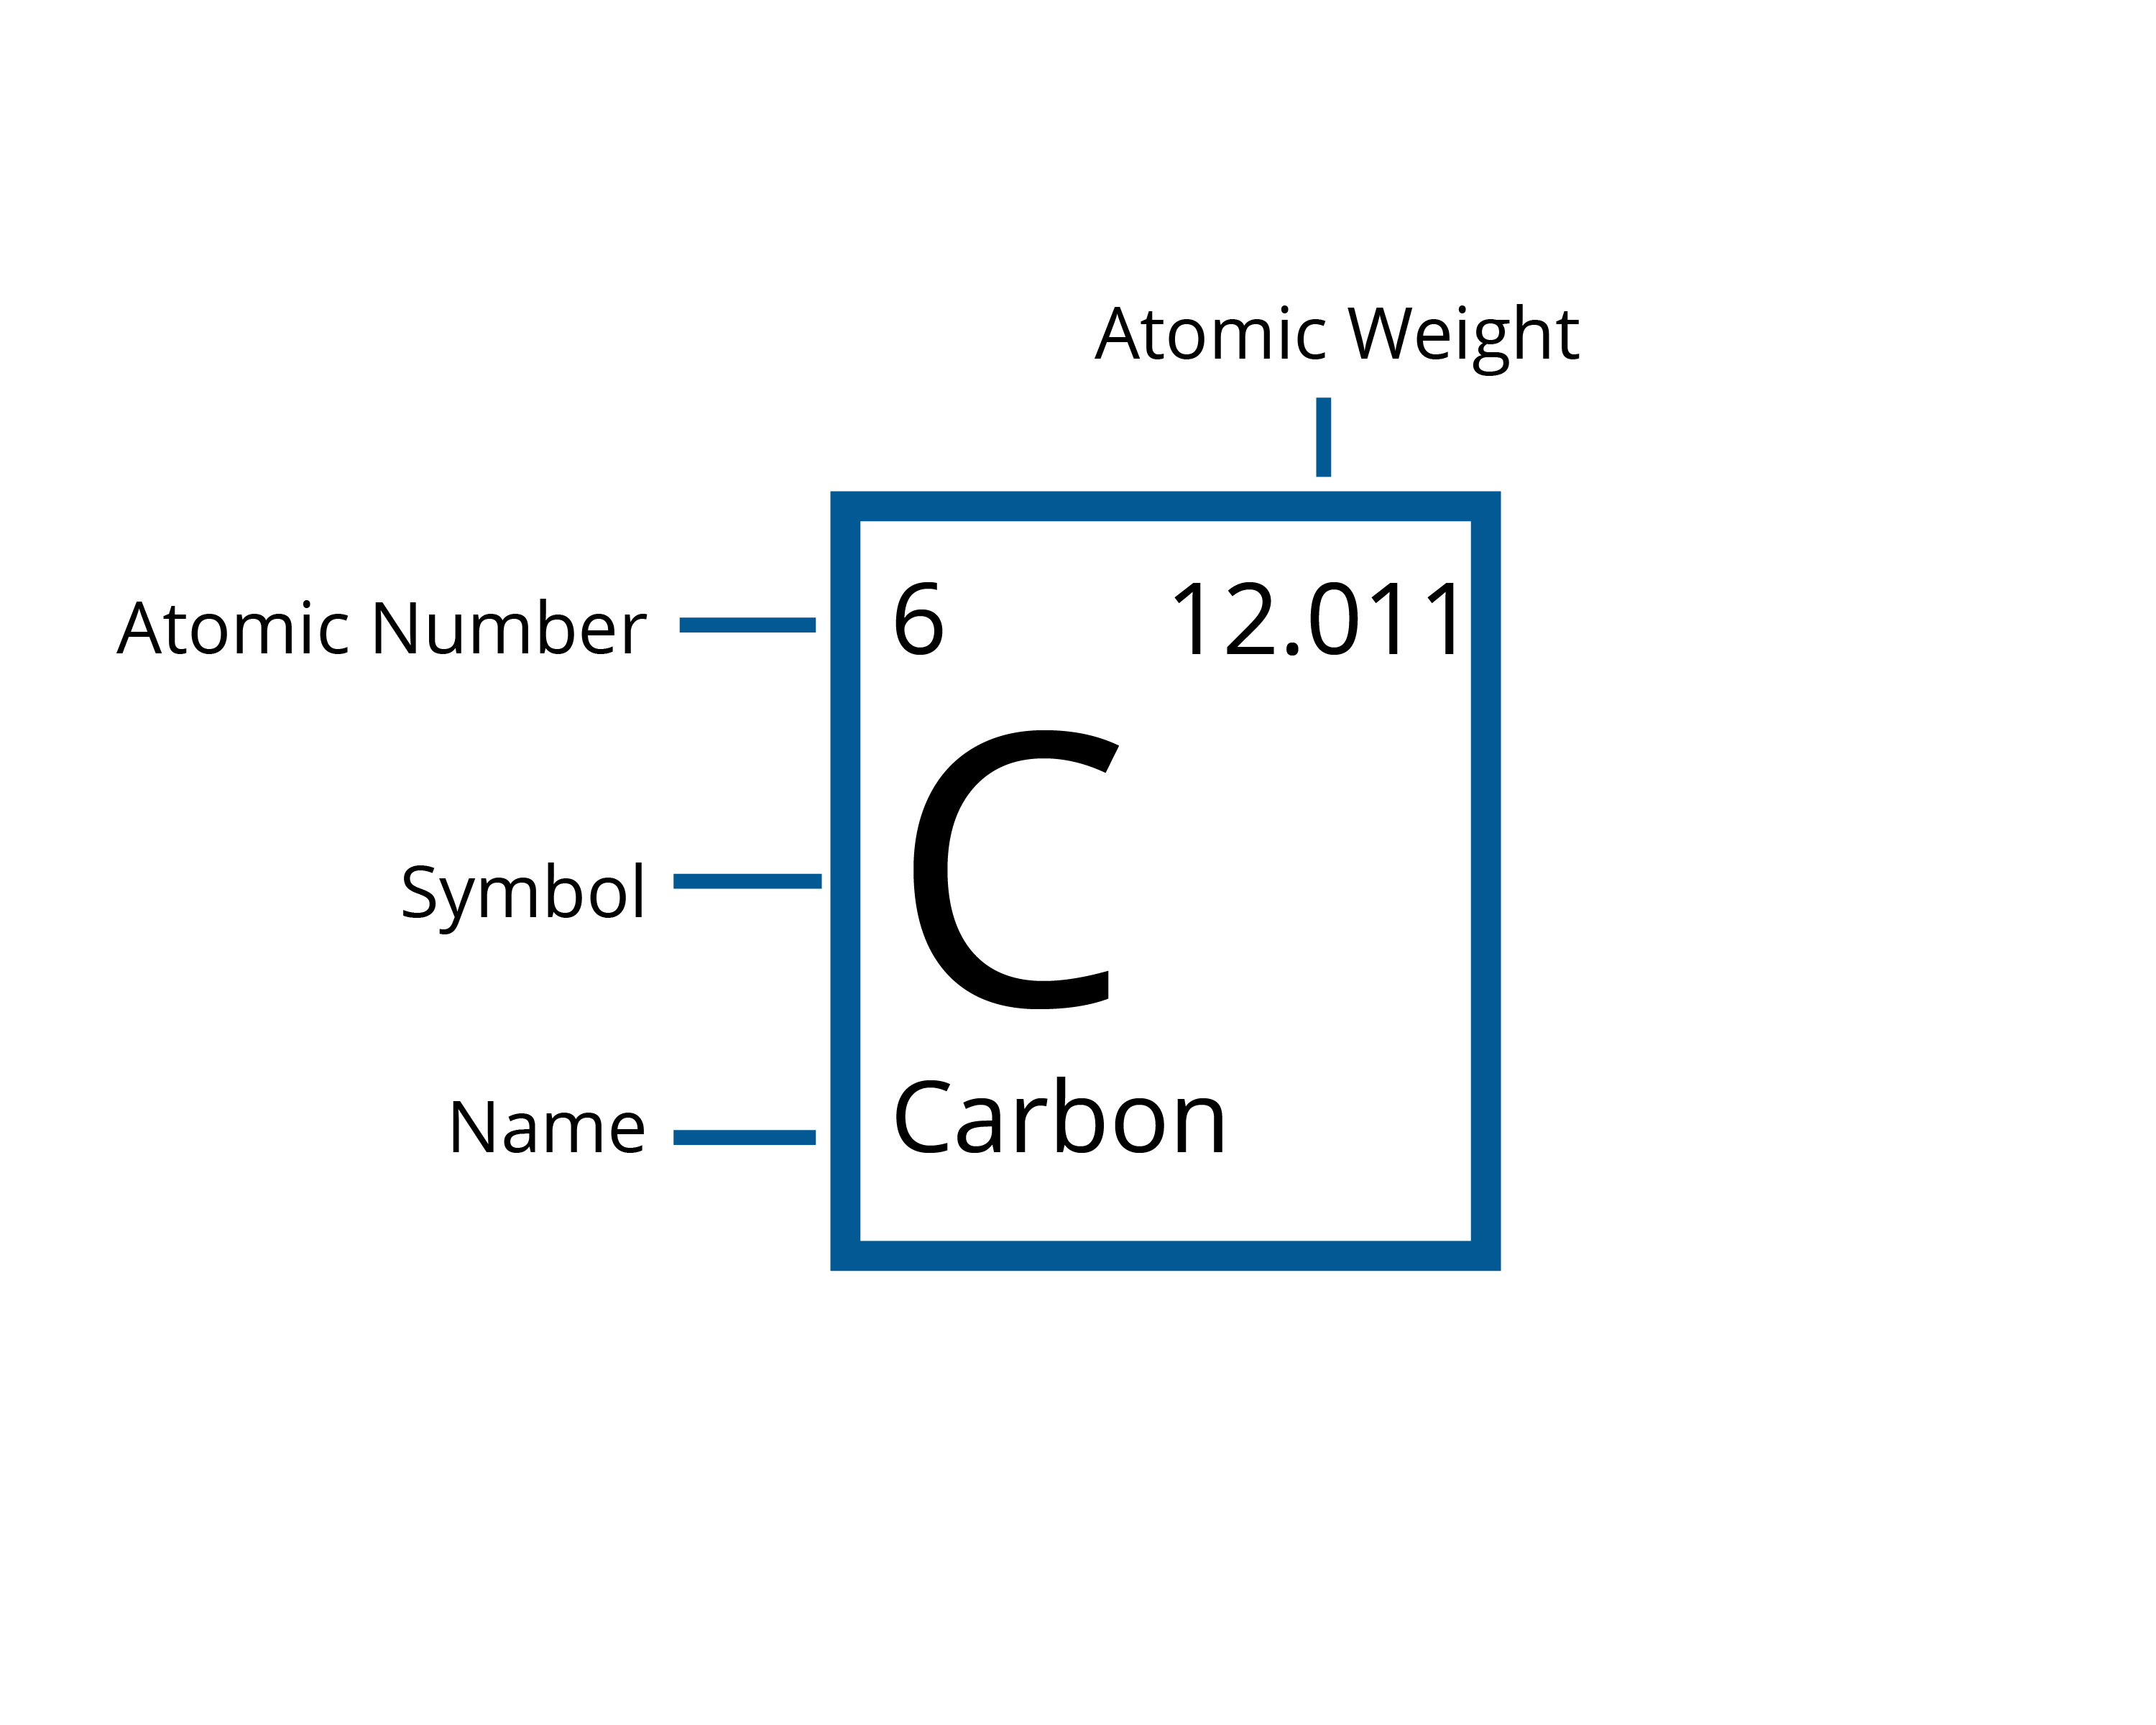
\includegraphics[width=0.8\textwidth]{element.png}

Look at the atomic mass of boron. About 80\% of all boron atoms have
six neutrons. The other 20\% have only 5 neutrons. This difference is why most boron atoms
have a mass of about 11 atomic mass units, but some have a mass of
about 10 atomic mass units. The atomic mass of boron is equivalent to the average
mass of a boron atom: 10.811.
% ADD: Talk about mass spectroscopy
%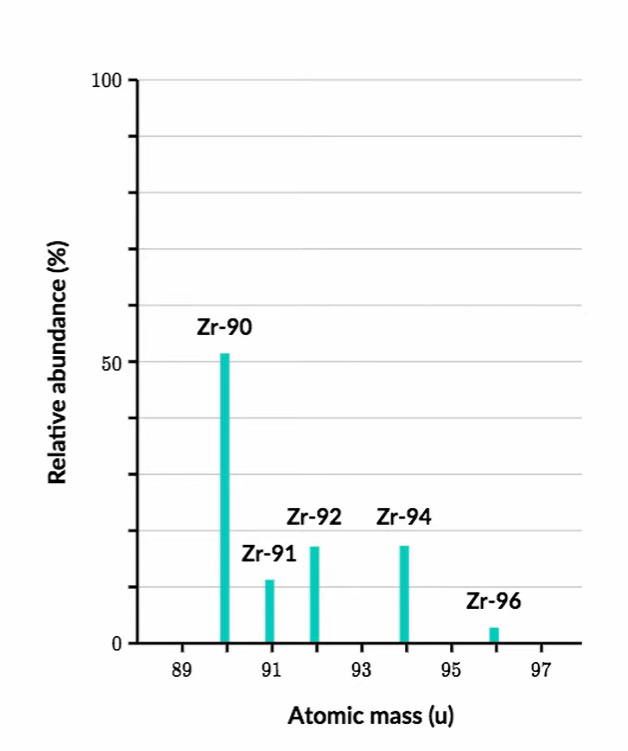
\includegraphics[width=0.75\textwidth]{KA_Mass_Spectroscopy_Zr.png}

\begin{Exercise}[title={Mass of a Water Molecule}, label=water_mass]

Using the periodic table, what is the average mass of one water molecule in atomic mass units?

\end{Exercise}
\begin{Answer}[ref=water_mass]

  The average hydrogen atom has a mass of 1.00794 atomic mass units.

  The average oxygen atom has a mass of 15.9994.

  $2 \times 1.00794 + 15.9994 = 18.01528$ atomic mass units.

\end{Answer}

\section{xfer from intro chapter} 
fixme integrate into this chapter
\subsection{Reading the Periodic Table}
The Periodic Table organizes what we know about the structure of different
elements. Each element has its own block or tile on the Periodic Table, and the
information on the tile tells us about the structure of that atom. Take a look at
the tile for carbon:

\begin{center}
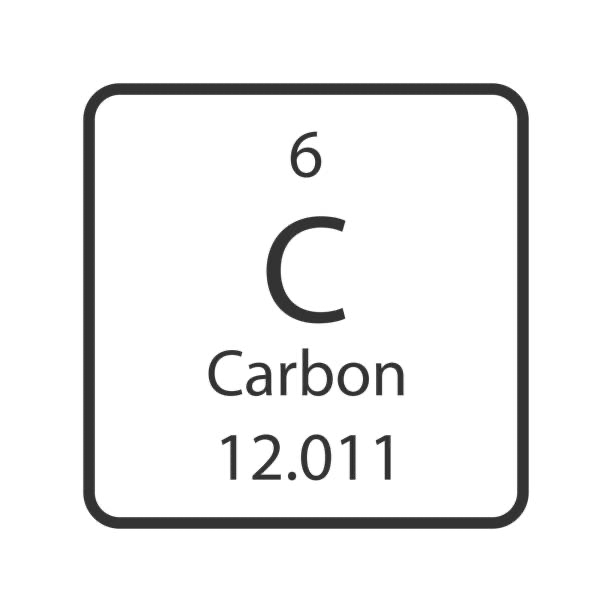
\includegraphics[width=2in]{carbon_tile.png}
\end{center}

The letter (or letters, as is the case for other elements) is the atomic symbol
for the element. There are two key numbers: the atomic number and the average
atomic mass. For carbon, the atomic number is 6 and the average atomic mass is
12.011. The atomic number tells us how many protons there are in the nucleus of
any atom of carbon. Since every element has a unique number of protons, every
element has a unique atomic number. All carbon atoms have 6 protons. The other
number is the average atomic mass - it tells us the weighted average of the
mass of all the carbons in the universe. When the average atomic mass is in
a whole number, as it is for polonium, it means that the element is very unstable.
As a result, the mass given is the mass of the most stable isotope (we'll talk
more about stability and isotopes below). On some periodic tables, the mass
number of the most stable isotope will be in parentheses or brackets. In
summary, if the larger number is a whole number, it is the mass number; if it
is a decimal (even if the decimal ends in .00), it is the average atomic mass,
which we will discuss further below.

\begin{center}
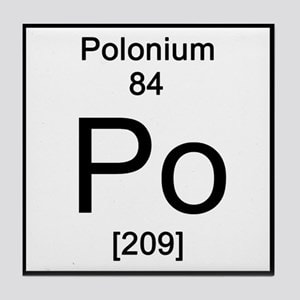
\includegraphics[width=2in]{polonium_tile.png}
\end{center}

The Royal Society of Chemistry has a very useful interactive periodic table:
periodic-table.rsc.org. We can use the periodic tile for an element to
determine the number of protons, electrons, and most common number of neutrons
for a neutral atom of that element (we'll explain why the periodic tile tells
us the "most common number of neutrons" below).

\textbf{Example}: State the atomic symbol for and the number of protons,
neutrons, and electrons in a neutral atom of plutonium.

\textbf{Solution}: The plutonium tile on your periodic table should look
something like this:
\begin{center}
   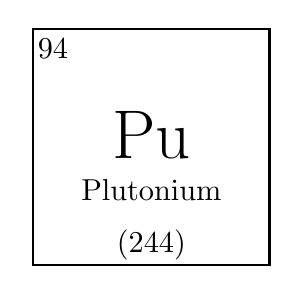
\begin{tikzpicture}
        \draw[black, thick] (-1.5, -1.5) rectangle (1.5,1.5);
        \node[font = \Huge] at (0,0.15) {Pu};
        \node[] at (-1.25, 1.25) {$94$};
        \node[] at (0, -0.55) {Plutonium};
        \node[] at (0, -1.25) {$(244)$};
    \end{tikzpicture}
\end{center}

[The information may be arranged differently, but you should at least see the
symbol and two numbers.] As you can see, the atomic symbol for plutonium is Pu.
Since its atomic number is 94, we know every atom of plutonium has 94 protons.
To know the number of electrons, we will take advantage of the fact that the
question is asking about a \textit{neutral} atom. This means there are the same
number of positive charges as negative charges. So, since there are 94 protons,
a neutral atom of plutonium must have 94 electrons (each proton has a +1 charge
and each electron has a -1 charge). Lastly, let's determine the number of
neutrons. The other number, 244, is the mass number. It represents the total
number of protons and neutrons in the nucleus. Since we know plutonium has 94
protons, we can find the number of neutrons by subtracting the atomic number
from the mass number:

\begin{center}
   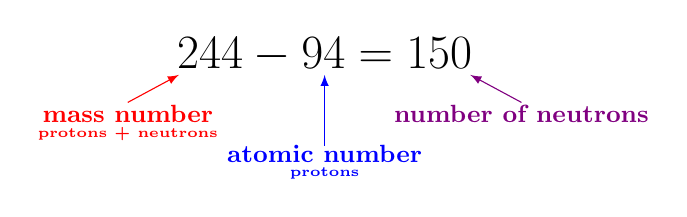
\begin{tikzpicture}
        \node[font = \LARGE] at (0,0) {$244 - 94 = 150$};
        \node[font = \small, red] at (-2.5, -0.75) {\textbf{mass number}};
        \node[font = \tiny, red] at (-2.5, -1) {\textbf{protons + neutrons}};
        \draw[red, -latex] (-2.5, -0.6) -- (-1.85, -0.25);
        \node[font = \small, blue] at (0, -1.25) {\textbf{atomic number}};
        \node[font = \tiny, blue] at (0, -1.5) {\textbf{protons}};
        \draw[blue, -latex] (0, -1.15) -- (0, -0.25);
        \node[font = \small, violet] at (2.5, -0.75) {\textbf{number of neutrons}};
        \draw[violet, -latex] (2.5, -0.6) -- (1.85, -0.25);
    \end{tikzpicture}
\end{center}

Therefore, an atom of plutonium has 150 neutrons. Now let's address how to find
the number of neutrons when the periodic tile shows an average atomic mass,
instead of a mass number. This occurs when there is more than one "version" of
an element. In the case of plutonium, there is only one version, which is why
the periodic tile shows a mass number instead of an average atomic mass. To
learn about average atomic mass, we will use carbon as an example.

Have you heard of carbon-14 dating? The phrase "carbon-14" refers to a rare
type of carbon that decays radioactively. By seeing how much carbon-14 has
decayed, scientists can estimate the age of organic materials, such as bone or
ash. Carbon-14 is a radioactive isotope (or version) of carbon. The 14 refers to
the mass number - the total amount of protons and neutrons in the nucleus
(sometimes, we shorten the isotope name by just using the atomic symbol, in
this case C-14). Isotopes are versions of an element with different numbers of
neutrons. The atomic number is the same for them all - they all have the same
number of protons. But the different number of neutrons causes different
isotopes to have different masses. Examine the models of carbon-12, carbon-13,
and carbon-14 below. What is different between them? What is the same?



You should have noticed that all three atoms have 6 protons and 6 electrons,
while they have differing numbers of neutrons. The most common isotope of carbon
is carbon-12, with 6 protons and 6 neutrons in its nucleus. Carbon-14, on the
other hand, has 8 neutrons, which makes the nucleus unstable, leading to
radioactive decay. The average atomic mass
is the weighted average of all the carbon atoms in existence. Since the vast
majority of carbon is carbon-12, the average atomic mass is very close to 12.
You cannot determine the mass number of an individual atom from the periodic
table; it only tells you the average of all the isotopes. However, especially
for light atoms (atoms in the first two rows of the periodic table), you can
usually determine the mass number of the most common isotope by rounding the
average atomic mass to the nearest whole number.

\textbf{Example}: Germanium has atomic symbol Ge. State the number of protons,
number of electrons, and most common number of neutrons in a neutral atom of
germanium.

\textbf{Solution}: Examining the periodic table, we see that germanium has an
atomic number of 32, which means a neutral atom of germanium has 32 protons and
32 electrons. The average atomic mass is 72.630, which rounds up to 73. So, the
most common isotope of germanium is Ge-73, which has $73 - 32 = 41$ neutrons.

\begin{Exercise}[title = {Determining Numbers of Subatomic Particles}, label = pne]
Use a periodic table to complete the table below (assume neutral atoms): %fixme wrap text for neutrons column

\begin{tabular}{|c|c|c|c|c|}
\hline\\
Element Name & Atomic Symbol & Protons & Most Common Number of Neutrons & Electrons\\\hline
 & Fr & & & \\\hline
 & & & & 33\\\hline
 Erbium & & & & \\\hline
  & & 48 & & \\\hline
\end{tabular}
\end{Exercise}

\begin{Answer}[ref = pne]
\begin{tabular}{|c|c|c|c|c|}
\hline\\
Element Name & Atomic Symbol & Protons & Most Common Number of Neutrons & Electrons\\\hline
 Francium & Fr & 87 & 136 & 87 \\\hline
 Arsenic & As & 33 & 42 & 33 \\\hline
 Erbium & Er & 68 & 99 & 68 \\\hline
 Cadmium & Cd & 48 & 64 & 48 \\\hline
\end{tabular}
\end{Answer}




\section{Heavy atoms aren't stable}

When you look at the periodic table, there are a surprisingly large
number of elements. You might be told to ``Drink milk so that you can
get the calcium you need.'' However, no one has told you ``You should
eat kale so that you get enough copernicium in your diet.''

Copernicium, with 112 protons and 173 neutrons, has only been observed
 in a lab. It is highly radioactive and unstable (meaning it decays). A copernicium
atom usually lives for less than a minute before decaying.
% ADD: Half Life

The largest stable element is lead, which has 82 protons and between
122 and 126 neutrons. Elements with lower atomic numbers than lead,
have at least one stable isotope, while elements with higher atomic numbers
than lead don't.

Bismuth, with an atomic number of 83, is \textit{almost} stable. In fact, most
bismuth atoms will live for billions of years before decaying!

\graphicspath{{../../Chapters/work_energy/en_US}}
\chapter{Work and Energy}

In this chapter, we are going to talk about how engineers define work
and energy. It frequently takes force to get work done. Let's start with thinking about the relationship between force and energy. As we learned earlier, Force is measured in
newtons, and one newton is equal to the force necessary to accelerate one
kilogram at a rate of $1 m/s^2$.

When you lean on a wall, you are exerting a force on the wall, but you
aren't doing any work. On the other hand, if you push a car for a mile,
you are clearly doing work. Work, to an engineer, is the force you
apply to something, as well as the distance that it moves, in the direction
of the applied force. We measure work in \textit{joules}. A joule is one
newton of force over one meter.\index{Joule}

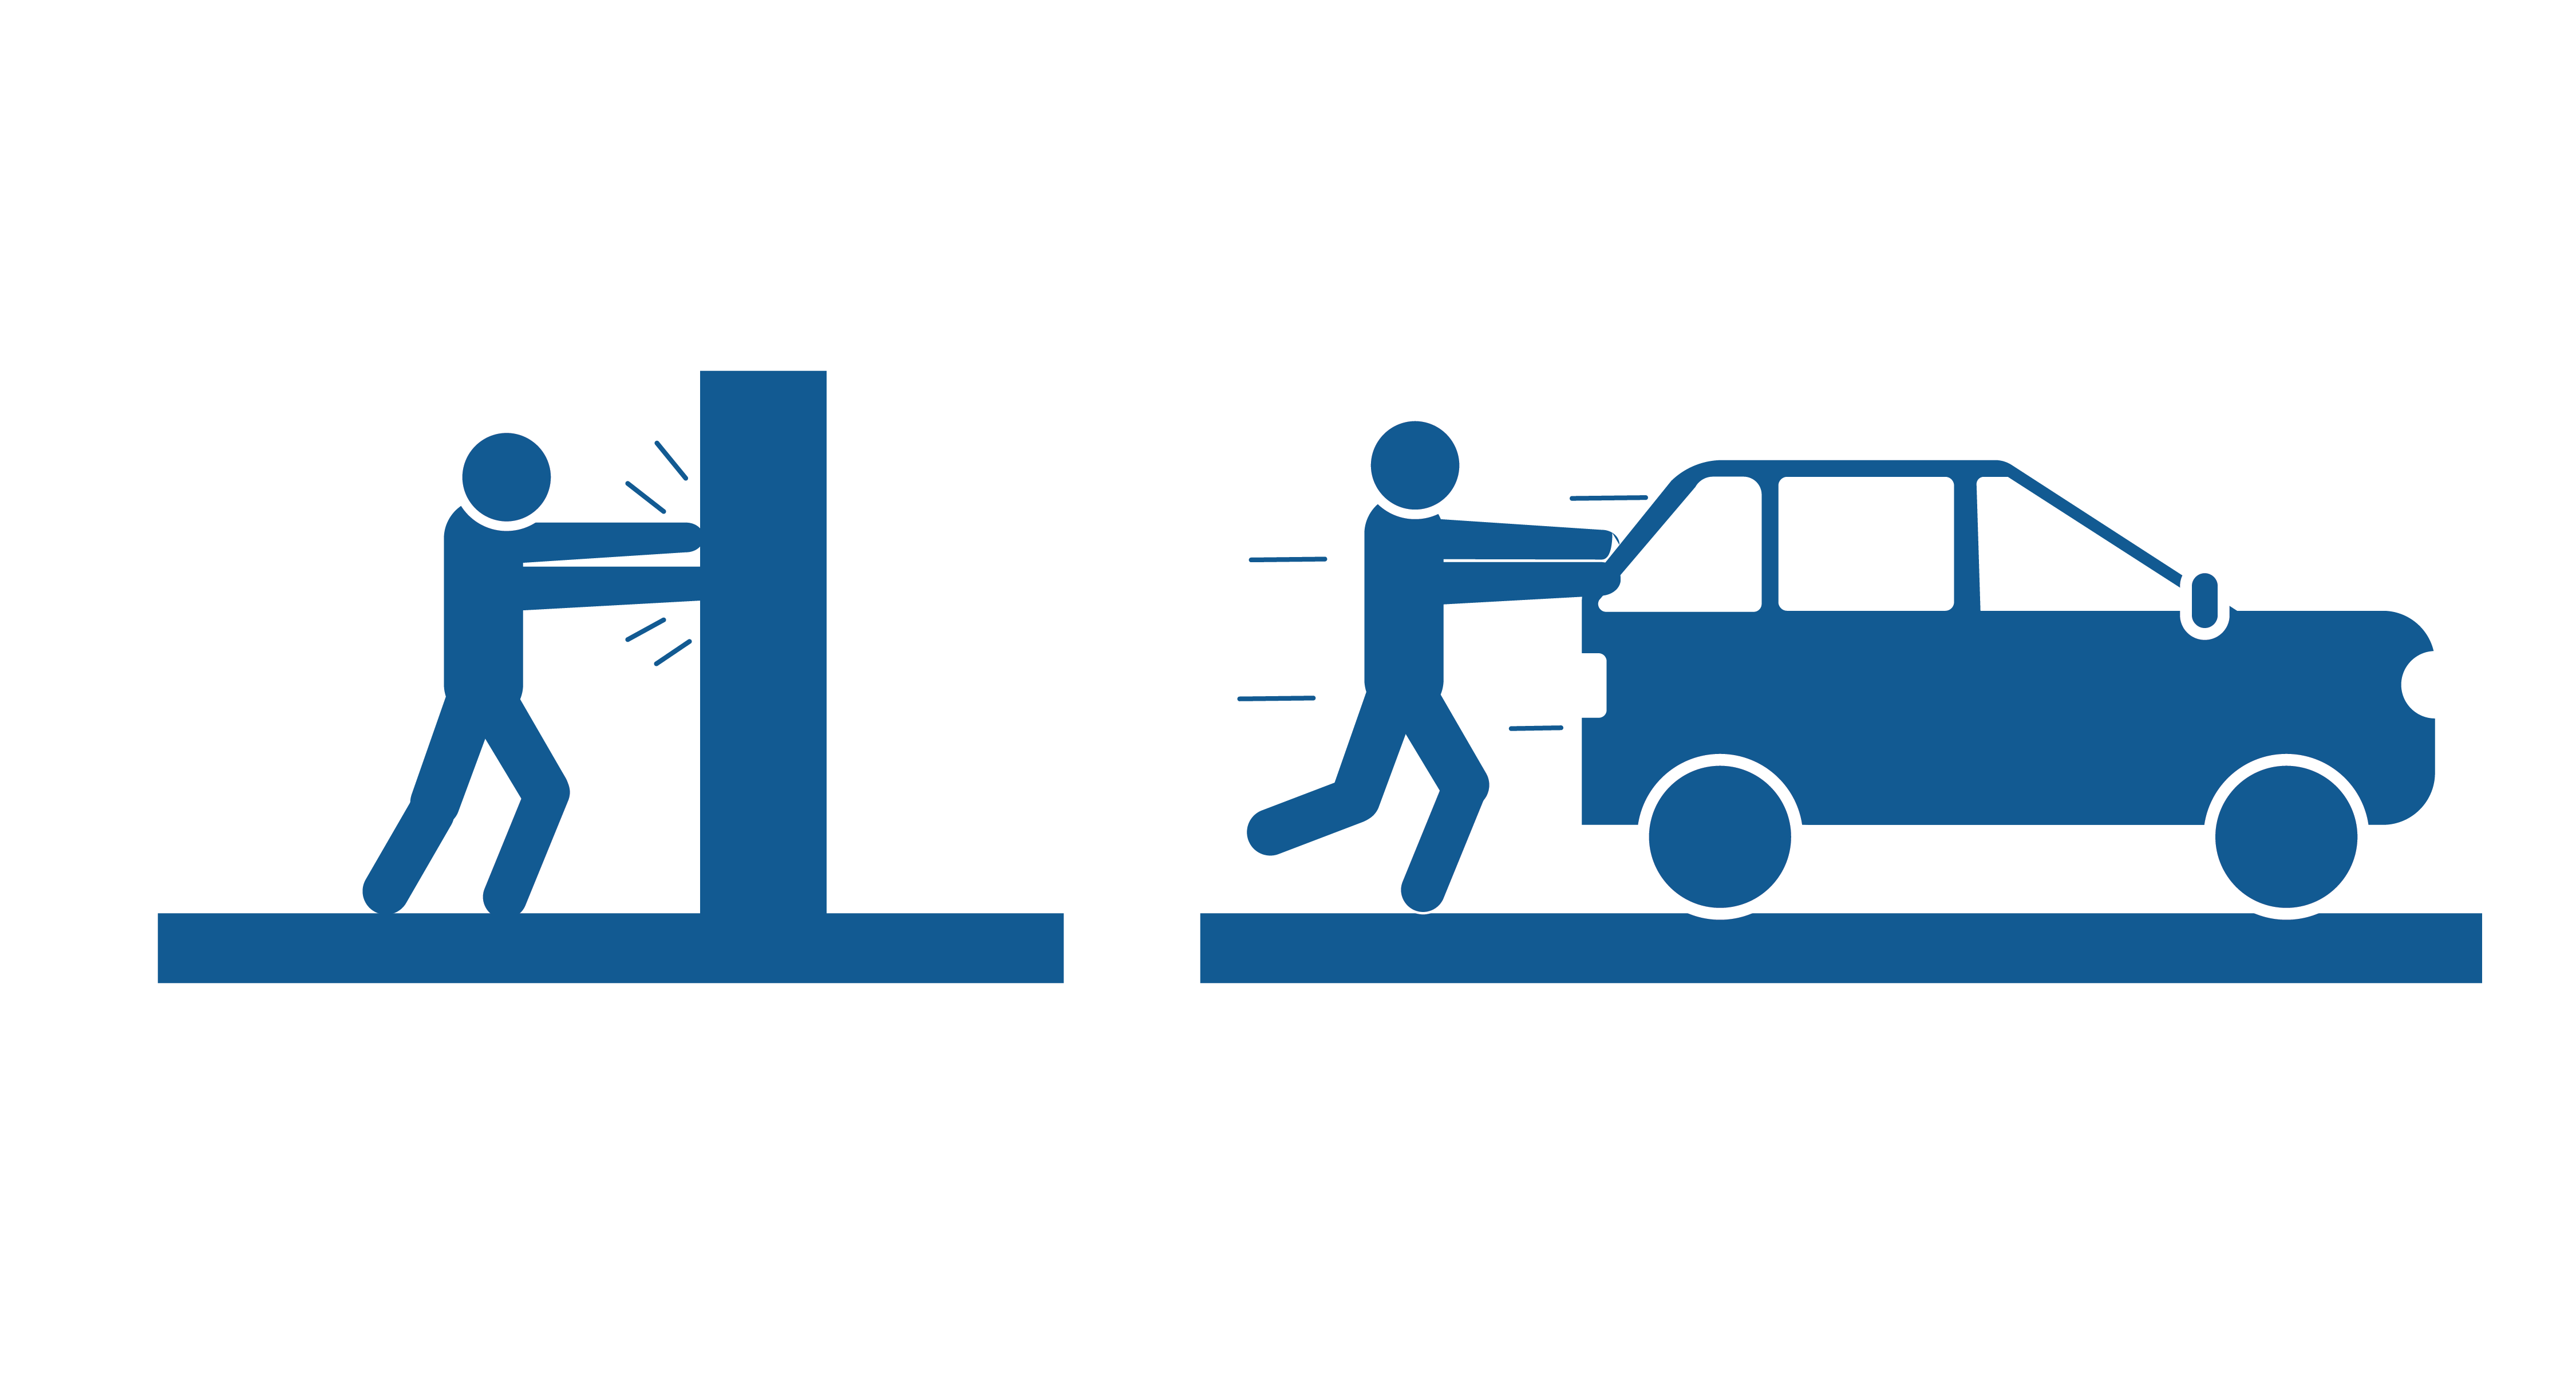
\includegraphics[width=1\textwidth]{workvsforce.png}

For example, if you push a car uphill with a force of 10 newtons for 12
meters, you have done 120 joules of work.\index{work}
% ADD: We can represent this with the equations, Work Energy Therom

Work is how energy is transferred from one thing to another. When you
push the car, you also burn sugars(energy of the body) in your blood. That energy is then
transferred to the car: after it has been pushed uphill.

Thus, we measure the energy something consumes or generates in 
units of work: joules, kilowatt-hours, horsepower-hours, foot-pounds,
BTUs( British Thermal Unit), and calories.

Let's go over a few different forms that energy can take.

Watch Khan Academy's \textbf{Changes in energy} at \url{https://www.khanacademy.org/science/ms-physics/x1baed5db7c1bb50b:energy/x1baed5db7c1bb50b:changes-in-energy/a/changes-in-energy}

\section{Forms of Energy}\index{energy!Forms of}

In this section we are going to learn about several different types of energy:
\begin{itemize}
\item Heat
\item Chemical Energy
\item Kinetic Energy
\item Gravitational Potential Energy
\end{itemize}

\subsection{Heat}\index{heat}

When you heat something, you are transferring energy to it. The BTU
 is a common unit for heat: One BTU is the
amount of heat required to raise the temperature of one pound of water,
by one degree. One BTU is about 1,055 joules. In fact, when you buy and sell
natural gas as fuel, it is priced by the BTU.\index{heat} \index{BTU}

\subsection{Electricity}\index{electricity}

Electricity is the movement of electrons. When you push electrons
through a space that resists their passage (like a light bulb),
energy is transferred from the power source ( a battery)
 into the source of the resistance.

Let's say your lightbulb consumes 60 watts of electricity, and you leave it on for 24 hours.
We would say that you have consumed 1.44 kilowatt hours or 3,600,000 joules.

Watch Khan Academy's \textbf{Introduction to charge} at \url{https://www.khanacademy.org/science/in-in-class10th-physics/in-in-electricity/in-in-electric-current-circuit/v/intro-to-charge}

\subsection{Chemical Energy}\index{chemical energy}

As mentioned early, some chemical reactions consume energy and some
produce energy. Thus, energy can be stored in the structure of a
molecule. When a plant uses photosynthesis to rearrange water and
carbon dioxide into a sugar molecule, it converts the energy in
the sunlight( solar energy) into chemical energy. Remember photosythesis is a process that releases energy.
Therefore, the sugar molecule has more chemical energy than the carbon dioxide and water molecules that were
used in its creation.
% ADD: photosythesis equation 
% KA: https://www.khanacademy.org/science/ap-biology/cellular-energetics/photosynthesis/a/intro-to-photosynthesis

In our diet, we measure this energy in \textit{kilocalories}. A
calorie is the energy necessary to raise one gram of water one degree
Celsius: it is about 4.19 joules. This is a very small unit: an apple
has about 100,000 calories( 100 kilocalories), so people working with food started
measuring everything in kilocalories.\index{calories}
% ADD: Conversion chapter should come before this chapter

Here is where things get confusing: People who work with food got tired of
saying ``kilocalories'', so they just started using ``Calorie'' to
mean 1,000 calories.  This has created terrible confusion over the
years. So if the C is capitalized, ``Calorie'' probably means kilocalorie.

\subsection{Kinetic Energy}\index{kinetic energy}

A mass in motion has energy. For example, if you are in a moving car
and you slam on the breaks, the energy from the motion of the
car will be converted into heat in the breaks and under the tires.

How much energy does the car have?
% ADD: section specifically about KE AND U, use roller coaster diagram

\begin{mdframed}[style=important, frametitle={Formula for Kinetic Energy}]

$$E = \frac{1}{2} m v^2$$

where $E$ is the energy in joules, $m$ is the mass in kilograms, and
$v$ is the speed in meters per second.

\end{mdframed}

\subsection{Gravitational Potential Energy}\index{potential energy!gravitational}

Watch Khan Academy's \textbf{Potential energy} at \url{https://youtu.be/oGzwVYPxKjg}

When you lift something heavy onto a shelf, you are giving it
\textit{potential energy}. The amount of energy that you transferred
to it is proportional to its weight and the height that you lifted it.

On the surface of the earth, gravity will accelerate a heavy object downward at
a rate of $9.8 m/s^2$.

\begin{mdframed}[style=important, frametitle={Formula for Gravitational Potential Energy}]
On earth, then, gravitational potential energy is given by

$$E = (9.8)mh$$


where $E$ is the energy in joules, $m$ is the mass of the object you
lifted, and $h$ is the height that you lifted it.

\end{mdframed}


There are other kinds of potential energy. For example, when you draw
a bow, you have given that bow potential energy. When you release it,
the potential energy is transferred to the arrow, which expresses it
as kinetic energy.
% ADD: section about KE and U

\section{Conservation of Energy}

The first law of thermodynamics says ``Energy is neither created nor
destroyed.''\index{energy!conservation of}

Energy can change forms: Your cells consume chemical energy to give
gravitational potential energy to a car you push up a hill. However, the total amount of
energy in a closed system stays constant.
% ADD: Create Systems chapter before introducing concept here

\begin{Exercise}[title={The Energy of Falling}, label=energy_falling]
  
A 5 kg cannonball falls off the top of a 3 meter ladder. Just before
it hits the floor, all of its gravitational potential energy has been
converted into kinetic energy.  How fast is the cannonball going when
it hits the floor?

\end{Exercise}
\begin{Answer}[ref=energy_falling]

  At the top of the ladder, the cannonball has $(9.8)(5)(3) = 147$ joules of potential energy.

  At the bottom, the kinetic energy $\frac{1}{2}(5)v^2$ must be equal
  to 147 joules. So $v^2 = \frac{294}{5}$.  Thus it is going about
  $7.7$ meters per second.

  (Yes, a tiny amount of energy is lost to air resistance. For a dense
  object moving at these relatively slow speeds, this energy is
  neglible.)
  
\end{Answer}


\section{Efficiency}


Watch Khan Academy's \textbf{Laws of thermodynamics} at \url{https://www.khanacademy.org/science/ap-biology/cellular-energetics/cellular-energy/a/the-laws-of-thermodynamics}

Although energy is always conserved as it moves through different
forms, scientists aren't always that good at controlling it.\index{efficiency}

For example, a car engine consumes the chemical energy in gasoline. Only
about 20\% of the energy consumed is used to turn the wheels.  Most of
the energy is actually lost as heat. If you run a car for a while, the engine
gets very hot and the exhaust going out the tailpipe turns hot.

A human is about 25\% efficient. Most of the loss is in the heat produced
during the chemical reactions that turns food into motion.
% ADD: Cellular Respiration
 
In general, if you are trying to increase efficiency in any system,
the solution is usually easy to identify because heat is produced. Reduce heat, Increase efficiency.

Light bulbs are an interesting case. To get the light of a 60 watt
incandescent bulb, you can use an 8 watt LED or a 16 watt fluorescent
light. Thus, we say that the LED light is much more efficient: If you
run both, the incandescent bulb will consume 1.44 kilowatt-hours. The
LED will consume only 0.192 kilowatt-hours.

Besides light, the incandescent bulb is producing a lot of heat. If it
is inside your house, what happens to the heat? It warms your house.

In the winter, when you want light and heat, the incandescent bulb is
100\% efficient!

In the summer, if you are running the air conditioner, the
incandescent bulb is worse than just ``inefficient at making light'' --
it is actually counteracting the air conditioner! 


\graphicspath{{../../Chapters/units_conversions/en_US}}
\chapter{Units and Conversions}

At this point, you are working with a lot of units: grams for weight,
joules for energy, newtons for force, meters for distance, seconds for
time, etc. For each type of measurement, there are several different
units; for example, distance can be measured in feet, miles,
and light-years.

\begin{mdframed}[style=important, frametitle={Some Equalencies}]

\begin{tabular}{r | l}
  \hline
  \multicolumn{2}{c}{\textbf{Distance}}\\
  1 mile & 1.6093 kilometers \\
  1 foot & 0.3048 meters \\
  1 inch & 2.54 centimeters \\
  1 light-year & $9.461 \times 10^{12}$ kilometers\\
  \hline
  \multicolumn{2}{c}{\textbf{Volume}}\\
  1 milliliter & 1 cubic centimeter \\
  1 quart & 0.9461 liters \\
  1 gallon & 3.7854 liters \\
  1 fluid ounce & 29.6 milliliters \\
  \hline
  \multicolumn{2}{c}{\textbf{Mass}}\\
  1 pound & 0.4535924 kilograms\\
  1 ounce & 0.4535924 grams\\
  1 metric ton & 1000 kilograms \\
  \hline
  \multicolumn{2}{c}{\textbf{Force}}\\
  1 newton & 1 kilogram meter per sec$^2$\\
  \hline
  \multicolumn{2}{c}{\textbf{Pressure}}\\
  1 pascal & 1 newton per square meter \\
  1 bar & 0.98692 atmosphere \\
  1 pound per square inch & 6897 pascals \\
  \hline
  \multicolumn{2}{c}{\textbf{Energy}}\\
  1 joule & 1 newton meter \\
  1 calorie & 4.184 joules \\
  1 kilowatt-hour & $3.6 \times 10^{6}$ joules  \\
\end{tabular}\index{units table}

(You don't need to memorize these! Just remember that this page is here.)
% Suggest putting this in the front or back of the book, maybe create a print out

\end{mdframed}

In the metric system, prefixes are often used to express a multiple. Here are the common prefixes:\index{metric system!prefixes}

\begin{mdframed}[style=important, frametitle={Common Prefixes for Metric Units}]

\begin{tabular}{r | l}
giga  & $\times 10^{9}$\\
mega  & $\times 10^{6}$\\
kilo  & $\times 10^{3}$\\
milli  & $\div 10^{3}$\\
micro  & $\div 10^{6}$\\
nano  & $\div 10^{9}$\\
\end{tabular}

(These are worth memorizing. Here's a mnemonic: ``King Henery Doesn't Usually Drink Chocolate Milk.'')
\end{mdframed}

\section{Conversion Factors}

Here is a really handy trick to remembering how to do conversions
between units.\index{conversion factors}

Often, you will be given a table like the one above, and someone will ask you
``How many miles are in 0.23 light-years?''  You know that 1 mile = 1.6093
kilometers and that 1 light-year is $9.461 \times 10^{12}$ kilometers.
How do you do the conversion?

The trick is to treat the two parts of the equality as a fraction that equals 1.  That is, you think:

$$\frac{1 \text{ miles}}{1.6093 \text{ km}} = \frac{1.6093 \text{ km}}{1 \text{ miles}} = 1$$

and

$$\frac{1 \text{ light-years}}{9.461 \times 10^{12} \text{ km}} = \frac{9.461 \times 10^{12} \text{ km}}{1 \text{ light-years}} = 1$$

We call these fractions \textit{conversion factors}.

Now, your problem is

$$0.23 \text{ light-years} \times \textit{ Some conversion factors} = ? \text{ miles}$$

Note that when you multiply fractions together, things in the numerators can cancel with things in the denominator:

$$\left( \frac{31\pi}{47} \right) \left( \frac{11}{37\pi}\right) = \left(\frac{31\cancel{\pi}}{47}\right) \left( \frac{11}{37\cancel{\pi}}\right) = \left(\frac{31}{47} \right) \left( \frac{11}{37} \right)$$

When working with conversion factors, you will do the same with the units:

\begin{multline*}
  0.23 \text{ light-years} \left( \frac{9.461 \times 10^{12} \text{ km}}{1 \text{ light-years}} \right) \left( \frac{1 \text{ miles}}{1.6093 \text{ km}} \right) = \\
  0.23 \text{ \cancel{light-years}} \left( \times \frac{9.461 \times 10^{12} \text{ \cancel{km}}}{1 \text{ \cancel{light-years}}} \right) \left( \frac{1 \text{ miles}}{1.6093 \text{ \cancel{km}}}\right) = \frac{(0.23)(9.461 \times 10^{12})}{1.6093} \text{ miles}$$
\end{multline*}

\begin{Exercise}[title={Simple Conversion Factors}, label=simple_conversion_factors]

  How many calories are in 4.5 kilowatt-hours?
  
\end{Exercise}
\begin{Answer}[ref=simple_conversion_factors]

  $$4.5 \text{ \cancel{kWh}} \left( \frac{3.6 \times 10^{6} \text{ \cancel{joules}}}{1 \text{ \cancel{kWh}}} \right) \left( \frac{1 \text{ calories}}{4.184 \text{ \cancel{joules}}}\right) = \frac{(4.5)(3.6 \times 10^6)}{4.184} = 1.08 \times 10^6 \text {calories}$$
  
\end{Answer}

\section{Conversion Factors and Ratios}

Conversion factors also work on ratios.  For example, if you are told
that a bug is moving 0.5 feet every 120 milliseconds. What is that in
meters per second?

The problem then is

$$\frac{0.5 \text{ feet}}{120 \text{ milliseconds}} = \frac{\text{? m}}{second}$$

So you will need conversion factors to replace the ``feet'' with ``meters'' and to replace ``milliseconds'' with ``seconds'':

\begin{multline*}
\left(\frac{0.5 \text{ \cancel{feet}}}{120 \text{ \cancel{milliseconds}}}\right) \left( \frac{0.3048 \text{ meters}}{1 \text{ \cancel{feet}}} \right) \left( \frac{ 1000 \text{ \cancel{milliseconds}}} {1 \text{ second}}\right) = \frac{(0.5)(0.3048)(1000)}{120}\text{ m/second}
\end{multline*}

\begin{Exercise}[title={Conversion Factors}, label=conversion_factors]

The hole in the bottom of the boat lets in 0.1 gallons every 2 minutes.  How many milliliters per second is that?
  
\end{Exercise}
\begin{Answer}[ref=onversion_factors]

  \begin{multline*}
    \frac{0.1 \text{ \cancel{gallons}}}{2 \text{ \cancel{minutes}}}
  \left( \frac{3.7854 \text{ \cancel{liters}}}{1 \text{ \cancel{gallons}}} \right)
  \left( \frac{1000 \text{ milliliters}}{1\text{ \cancel{liters}}}\right)
  \left( \frac{1 \text{ \cancel{minutes}}}{60 \text{ seconds}} \right) = \\
  \frac{(0.1)(3.7854)(1000)}{(2)(60)} \text{ ml/second} = 3.1545 \text{ ml/second}
  \end{multline*}
  
\end{Answer}

\section{When Conversion Factors Don't Work}

Conversion factors only work when the units being converted are
proportional to each other. Gallons and liters, for example, are
proportional to each other: If you have $n$ gallons, you have $n
\times 3.7854$ liters.

Degrees celsius and degrees farenheit are \textit{not} proportional to
each other.  If your food is $n$ degrees celsius, it is $n \times
\frac{9}{5} + 32$ degrees farenheit.  You can't use conversion factors
to convert celsius to farenheit.

Watch Khan Academy's video on this at \url{https://www.khanacademy.org/test-prep/sat/x0a8c2e5f:untitled-652/x0a8c2e5f:problem-solving-and-data-analysis-lessons-by-skill/a/gtp--sat-math--article--units--lesson}


\graphicspath{{../../Chapters/simple_machines/en_US}}
\chapter{Simple Machines}

As mentioned earlier, physicists define work as the force applied times the distance over which it is applied. For example, if you push your car 100 meters with a force of 17 newtons, you have done 1700 joules of work.

Humans have long needed to move heavy objects, so many centuries ago, we developed simple machines to reduce the amount of force necessary to perform such tasks. These include:

\begin{itemize}
    \item Levers
    \item Pulleys
    \item Inclined planes
    \item Gears
    \item Hydraulics
    \item Screws
\end{itemize}

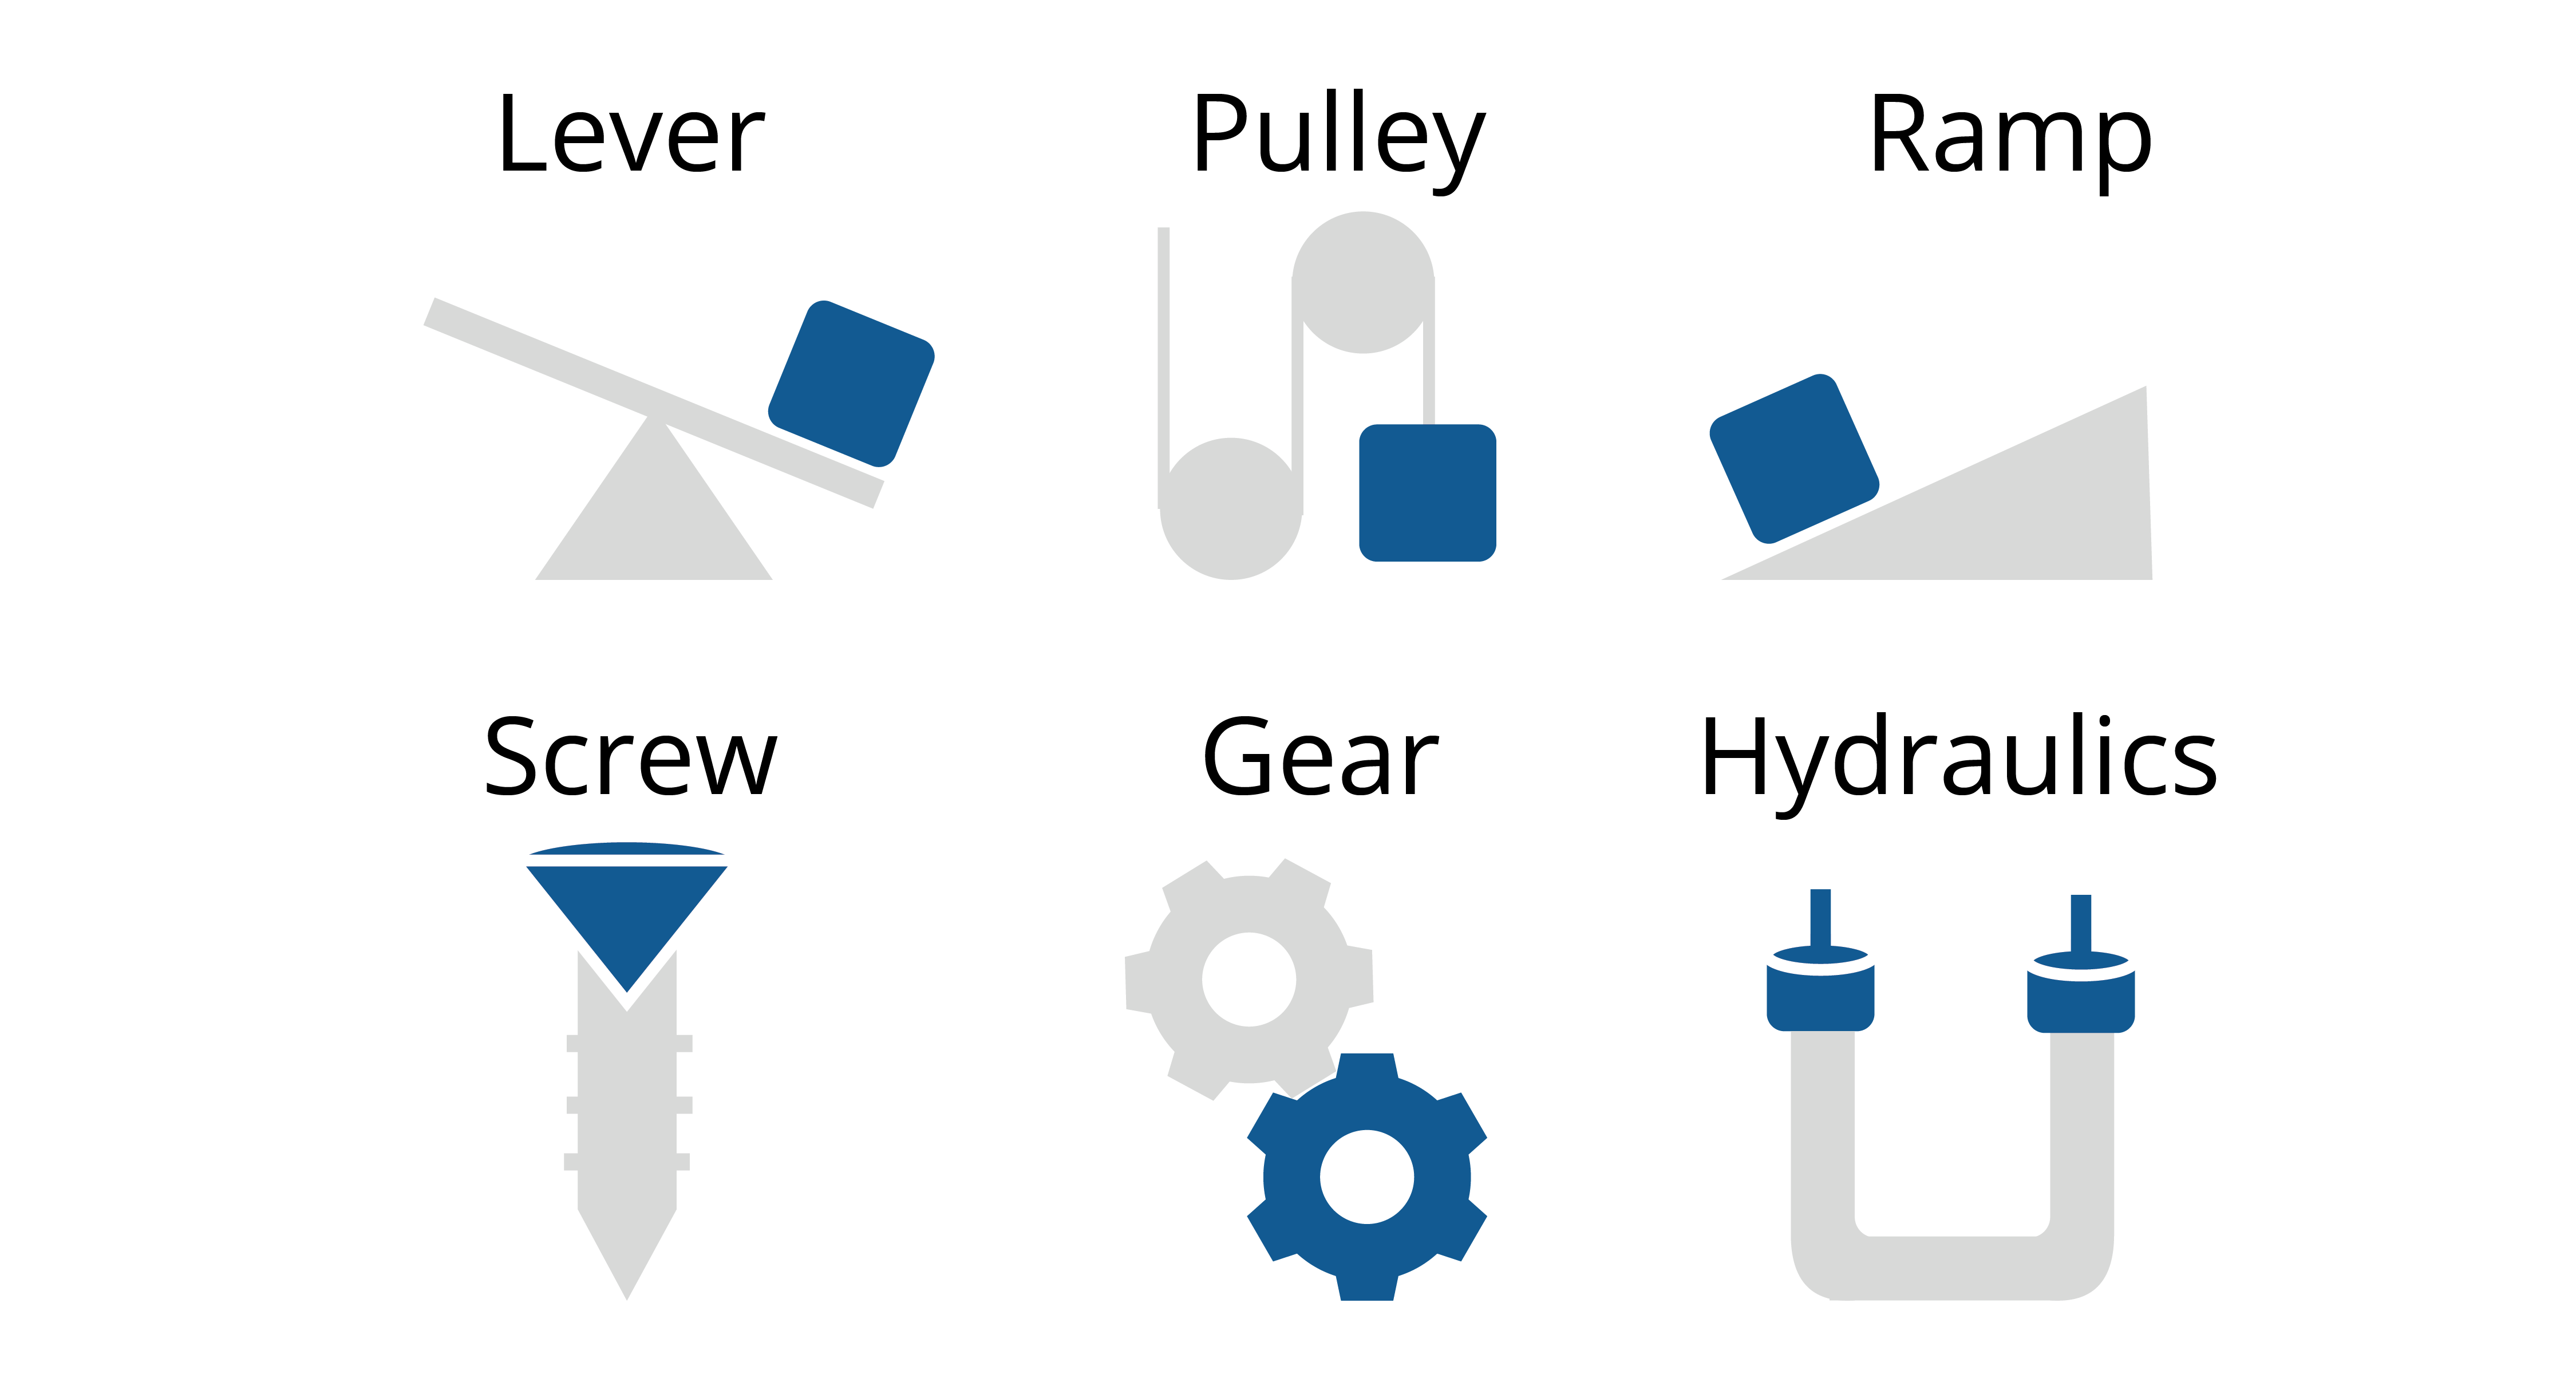
\includegraphics[width=\textwidth]{simplemachines.png}

While these machines can reduce the force needed, they do not change the total amount of work that must be done. For instance, if the force is reduced by a factor of three, the distance over which the force must be applied increases by the same factor.

The term \textit{mechanical advantage} refers to the increase in force achieved by using these machines.

\section{Levers}

A lever pivots on a fulcrum. To decrease the necessary force, the load is placed closer to the fulcrum than where the force is applied.

Physicists also discuss the concept of \newterm{torque} created by a force. When you apply force to a lever, the torque is the product of the force you exert and the distance from the point of rotation.

Torque is typically measured in newton-meters.

To balance two torques, the products of force and distance must be equal. Thus, assuming the forces are applied in the correct direction, the equation becomes:

\[
R_L F_L = R_A F_A
\]

where \( R_L \) and \( R_A \) represent the distances from the fulcrum to where the load’s force and the applied force are exerted, respectively, and \( F_L \) and \( F_A \) are the magnitudes of the forces.

\begin{Exercise}[title={Lever}, label=lever]
Paul, who weighs 70 kilograms, sits on a see-saw 4 meters from the fulcrum. Jan, who weighs 50 kilograms, wishes to balance the see-saw. How far should Jan sit from the fulcrum?
\end{Exercise}
\begin{Answer}[ref=lever]
Paul exerts a force of \( 70 \times 9.8 = 686 \) newtons at a distance of 4 meters from the fulcrum, creating a torque of \( 686 \times 4 = 2744 \) newton-meters. Jan exerts a force of \( 50 \times 9.8 = 490 \) newtons.

Let \( r \) be the distance from the fulcrum to Jan's seat. To balance the torques:

\[
490 \times r = 2744
\]

Solving for \( r \), we find \( r = \frac{2744}{490} \approx 5.6 \) meters.
\end{Answer}

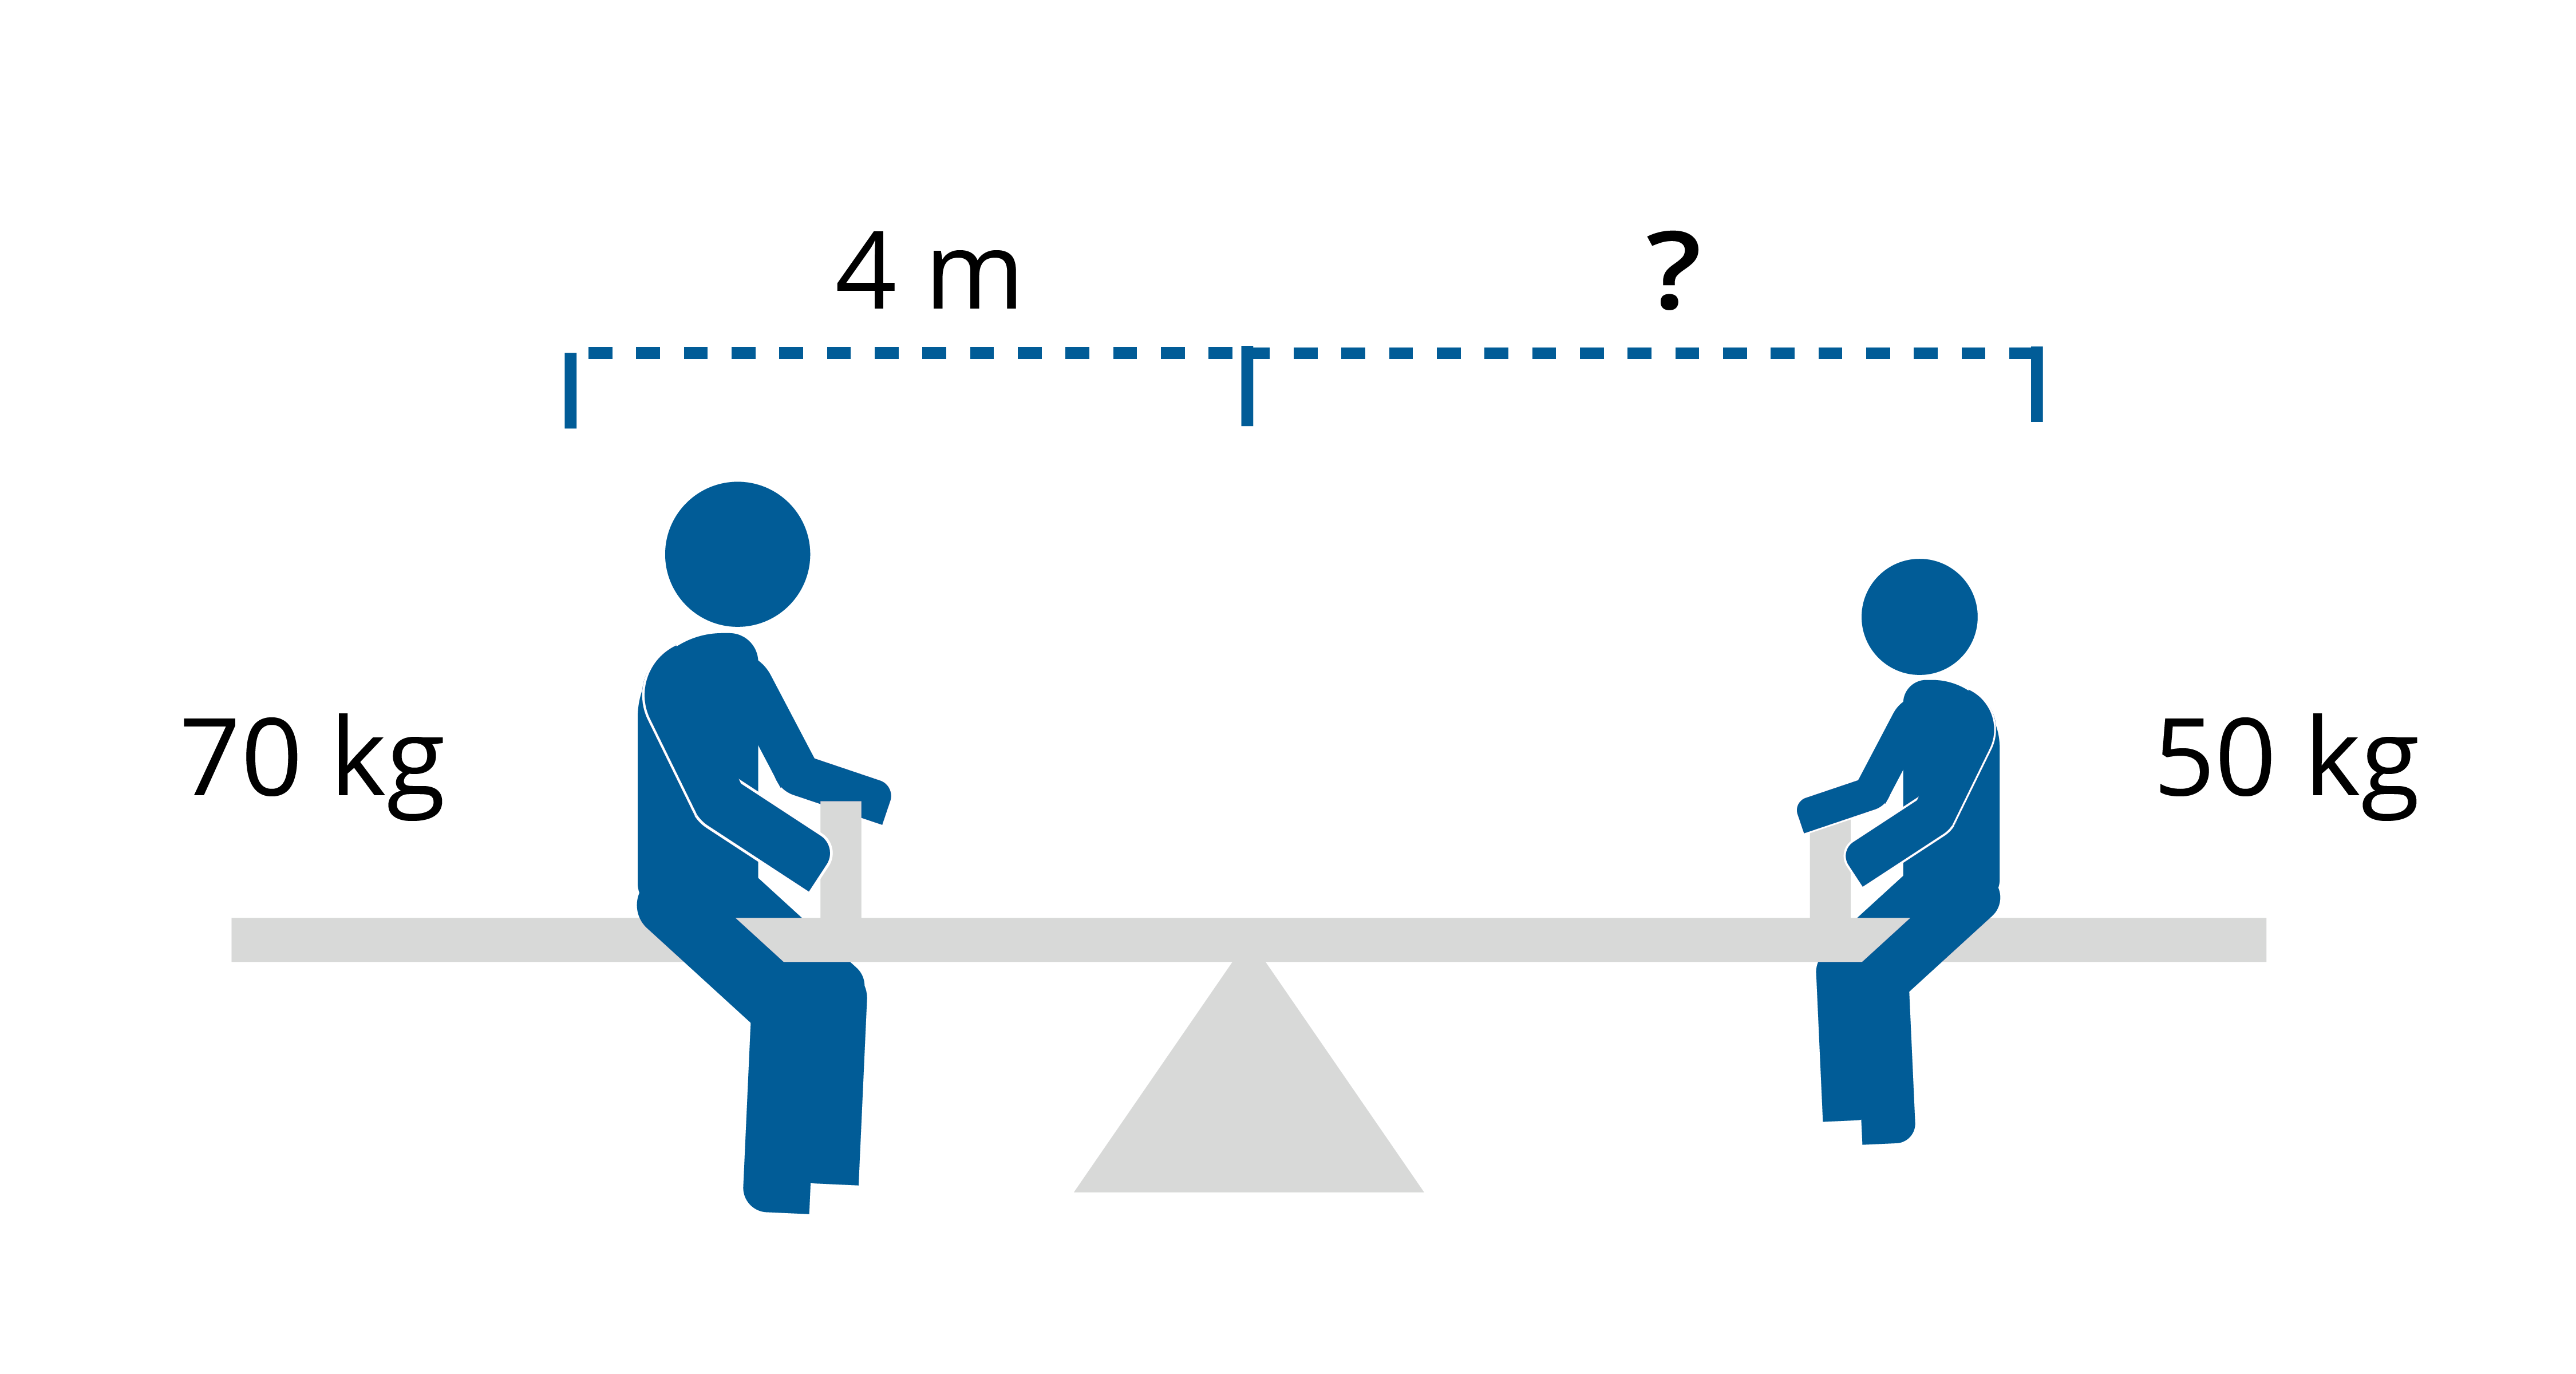
\includegraphics[width=0.6\textwidth]{seesaw.png}

\section{Inclined Planes}

Inclined planes, or ramps, allow you to roll or slide objects to a higher level. Steeper ramps require less mechanical advantage. For instance, it is much easier to roll a ball up a wheelchair ramp than a skateboard ramp.

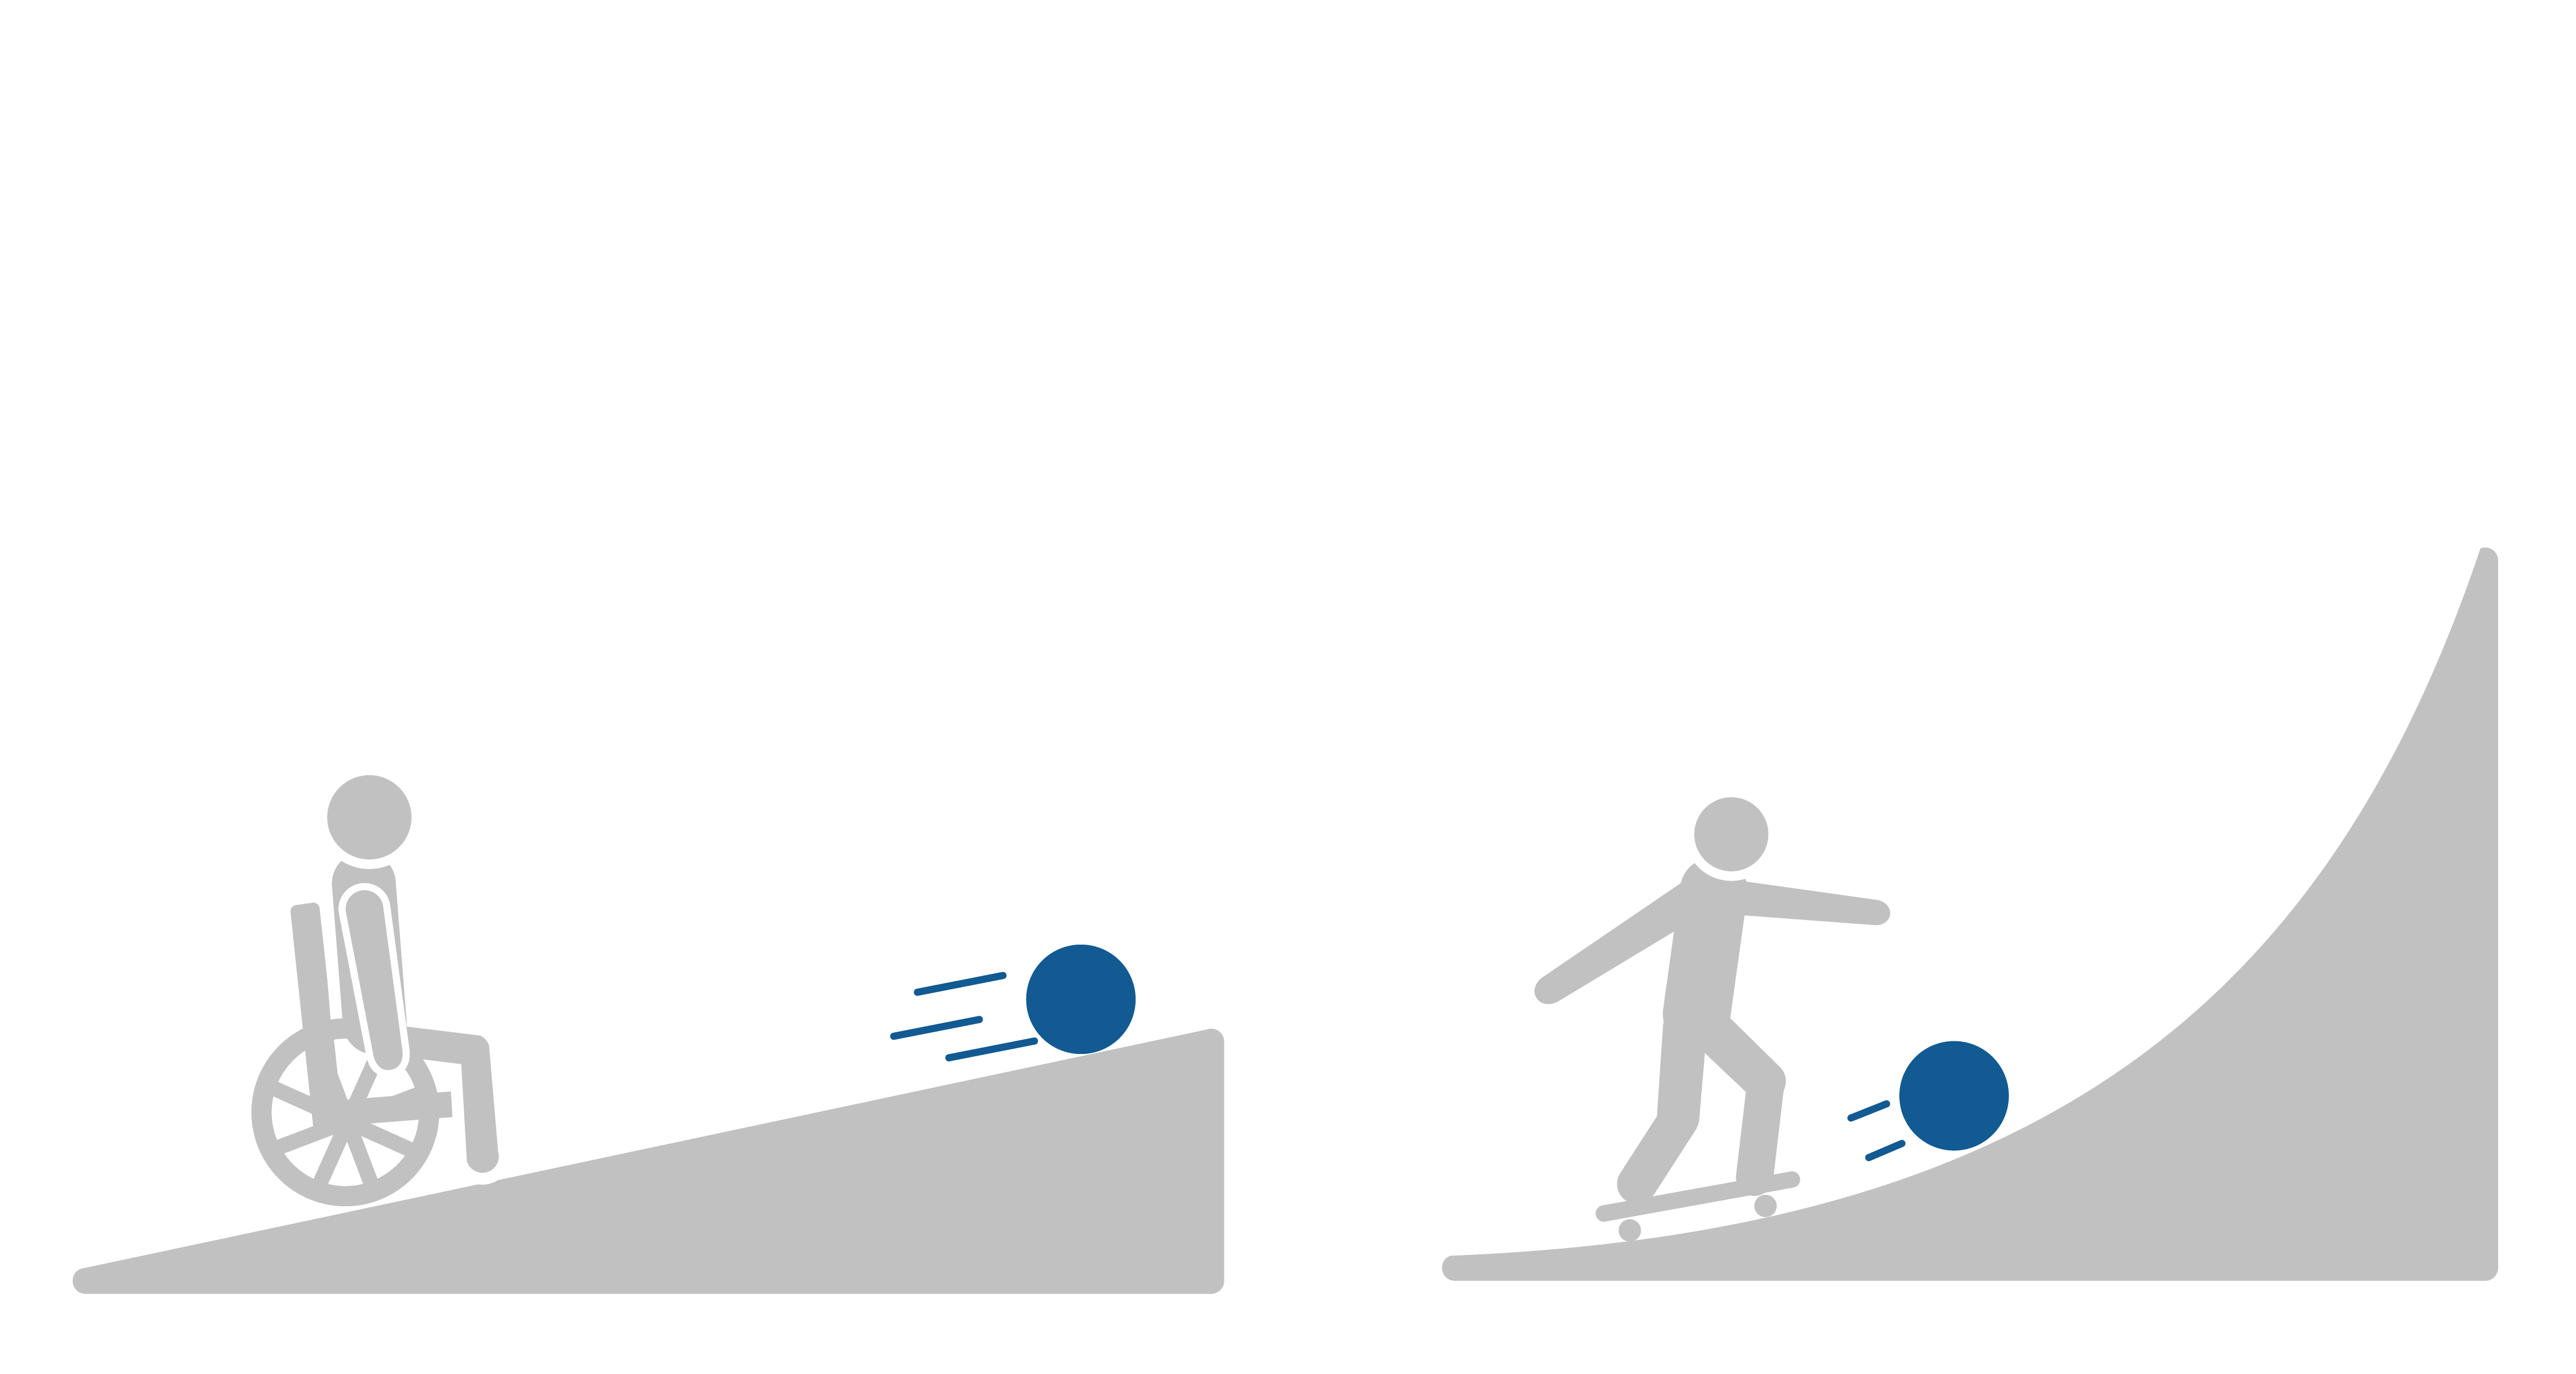
\includegraphics[width=\textwidth]{rampcomparison.png}

Assuming the incline has a constant steepness, the mechanical advantage is equal to the ratio of the length of the inclined plane to the height it rises.

If friction is neglected, the force required to push a weight up the inclined plane is given by:

\[
F_A = \frac{V}{L} F_G
\]

where \( F_A \) is the applied force, \( L \) is the length of the inclined plane, \( V \) is the vertical rise, and \( F_G \) is the gravitational force acting on the mass.

(We will discuss sine function later, but in case you're familiar with it, note that:

\[
\frac{V}{L} = \sin{\theta}
\]

where \( \theta \) is the angle between the inclined plane and the horizontal surface.)

\begin{Exercise}[title={Ramp}, label=ramp]
A barrel of oil weighs 136 kilograms. You can apply a force of up to 300 newtons. You need to get the barrel onto a platform that is 2 meters high. What is the shortest length of inclined plane you can use?
\end{Exercise}
\begin{Answer}[ref=ramp]
The weight of the barrel is \( 136 \times 9.8 = 1332.8 \) newtons.

Let \( L \) be the length of the inclined plane. The force needed to push the barrel up is related by:

\[
300 = \frac{2}{L} \times 1332.8
\]

Solving for \( L \), we find \( L = \frac{2 \times 1332.8}{300} \approx 8.885 \) meters.
\end{Answer}

\section{Gears}

Gears have teeth that mesh with each other. When you apply torque to one gear, it transfers torque to the other. The resulting torque is increased or decreased depending on the ratio of the number of teeth on the gears.

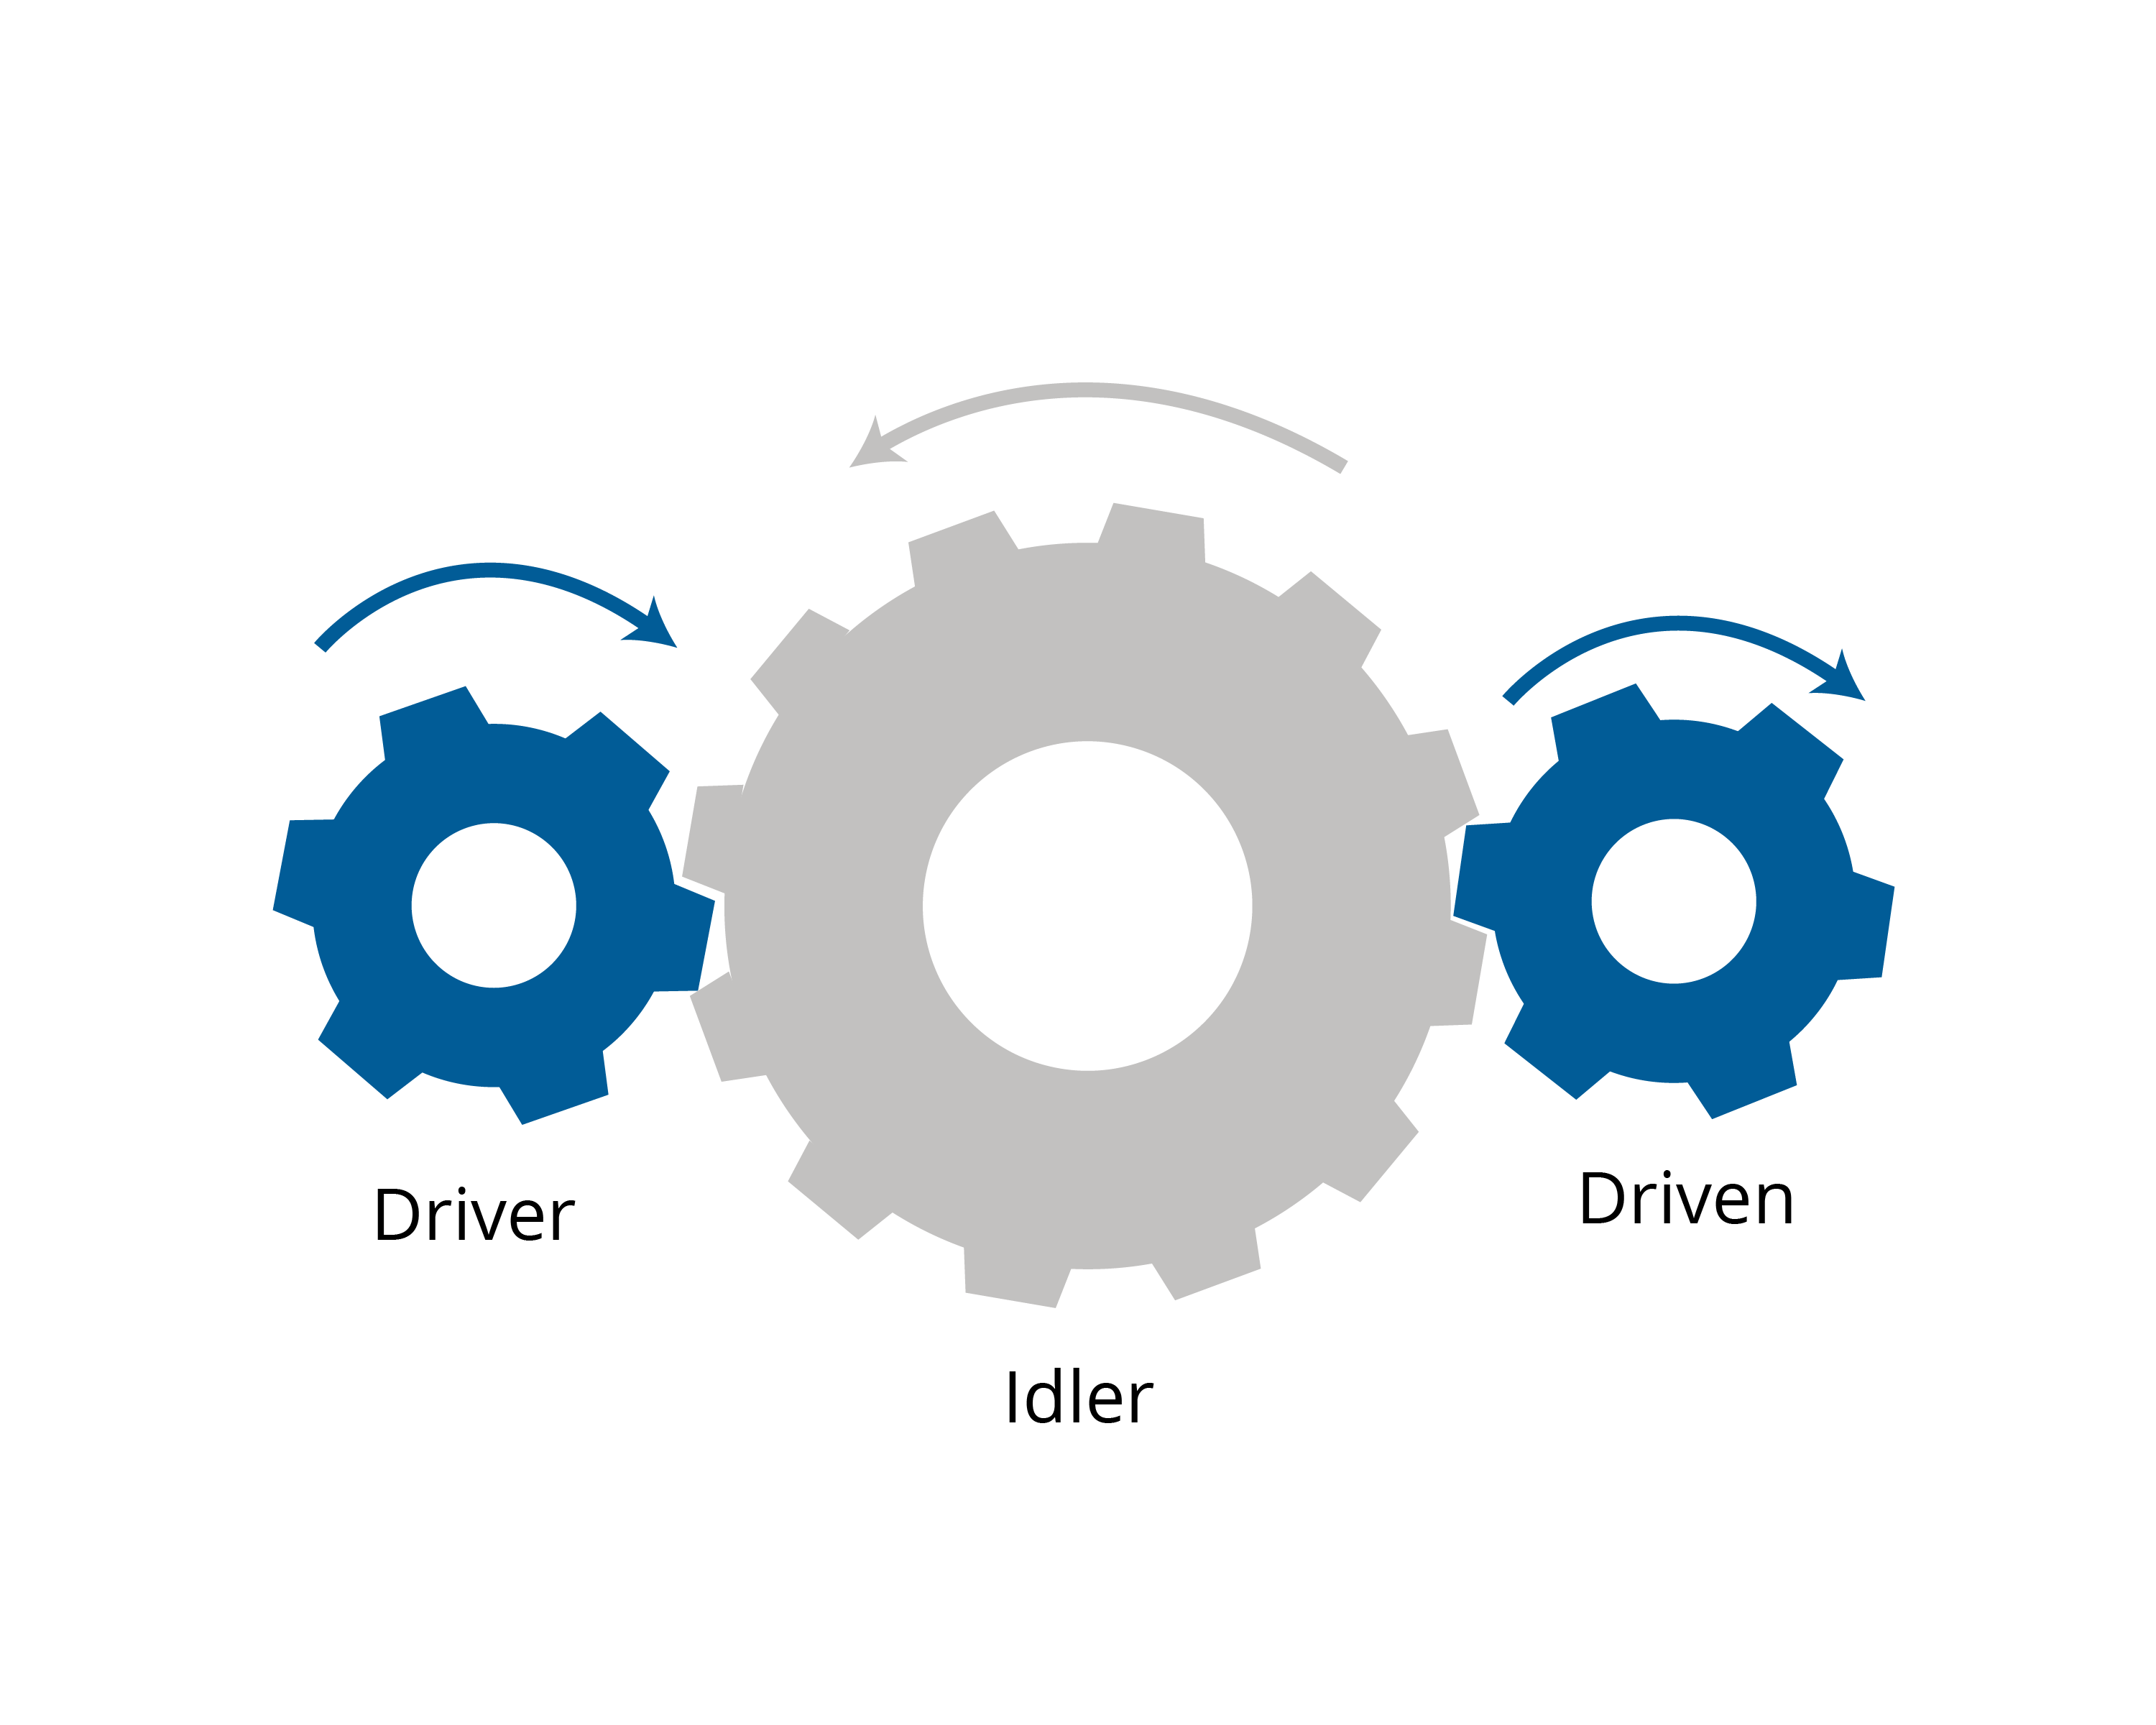
\includegraphics[width=0.7\textwidth]{gearsNew.png}

If \( N_A \) is the number of teeth on the gear you are turning with a torque of \( T_A \), and \( N_L \) is the number of teeth on the gear it is turning, the resulting torque is:

\[
T_L = \frac{N_A}{N_L} T_A
\]

\begin{Exercise}[title={Gears}, label=gear]
In a bicycle, the goal is not always to gain mechanical advantage, but to spin the pedals slower while applying more force.

You like to pedal your bike at 70 revolutions per minute. The chainring connected to your pedals has 53 teeth. The circumference of your tire is 2.2 meters. You want to ride at 583 meters per minute.

How many teeth should the rear sprocket have?
\end{Exercise}
\begin{Answer}[ref=gear]
The equation relating these quantities is:

\[
583 = 70 \times 2.2 \times \frac{53}{n}
\]

Solving for \( n \), we find \( n = 14 \) teeth.
\end{Answer}

\section{Hydraulics}

In a hydraulic system, such as a car's braking system, you exert force on a piston filled with fluid. The fluid transmits this pressure into another cylinder, where it pushes yet another piston that moves the load.

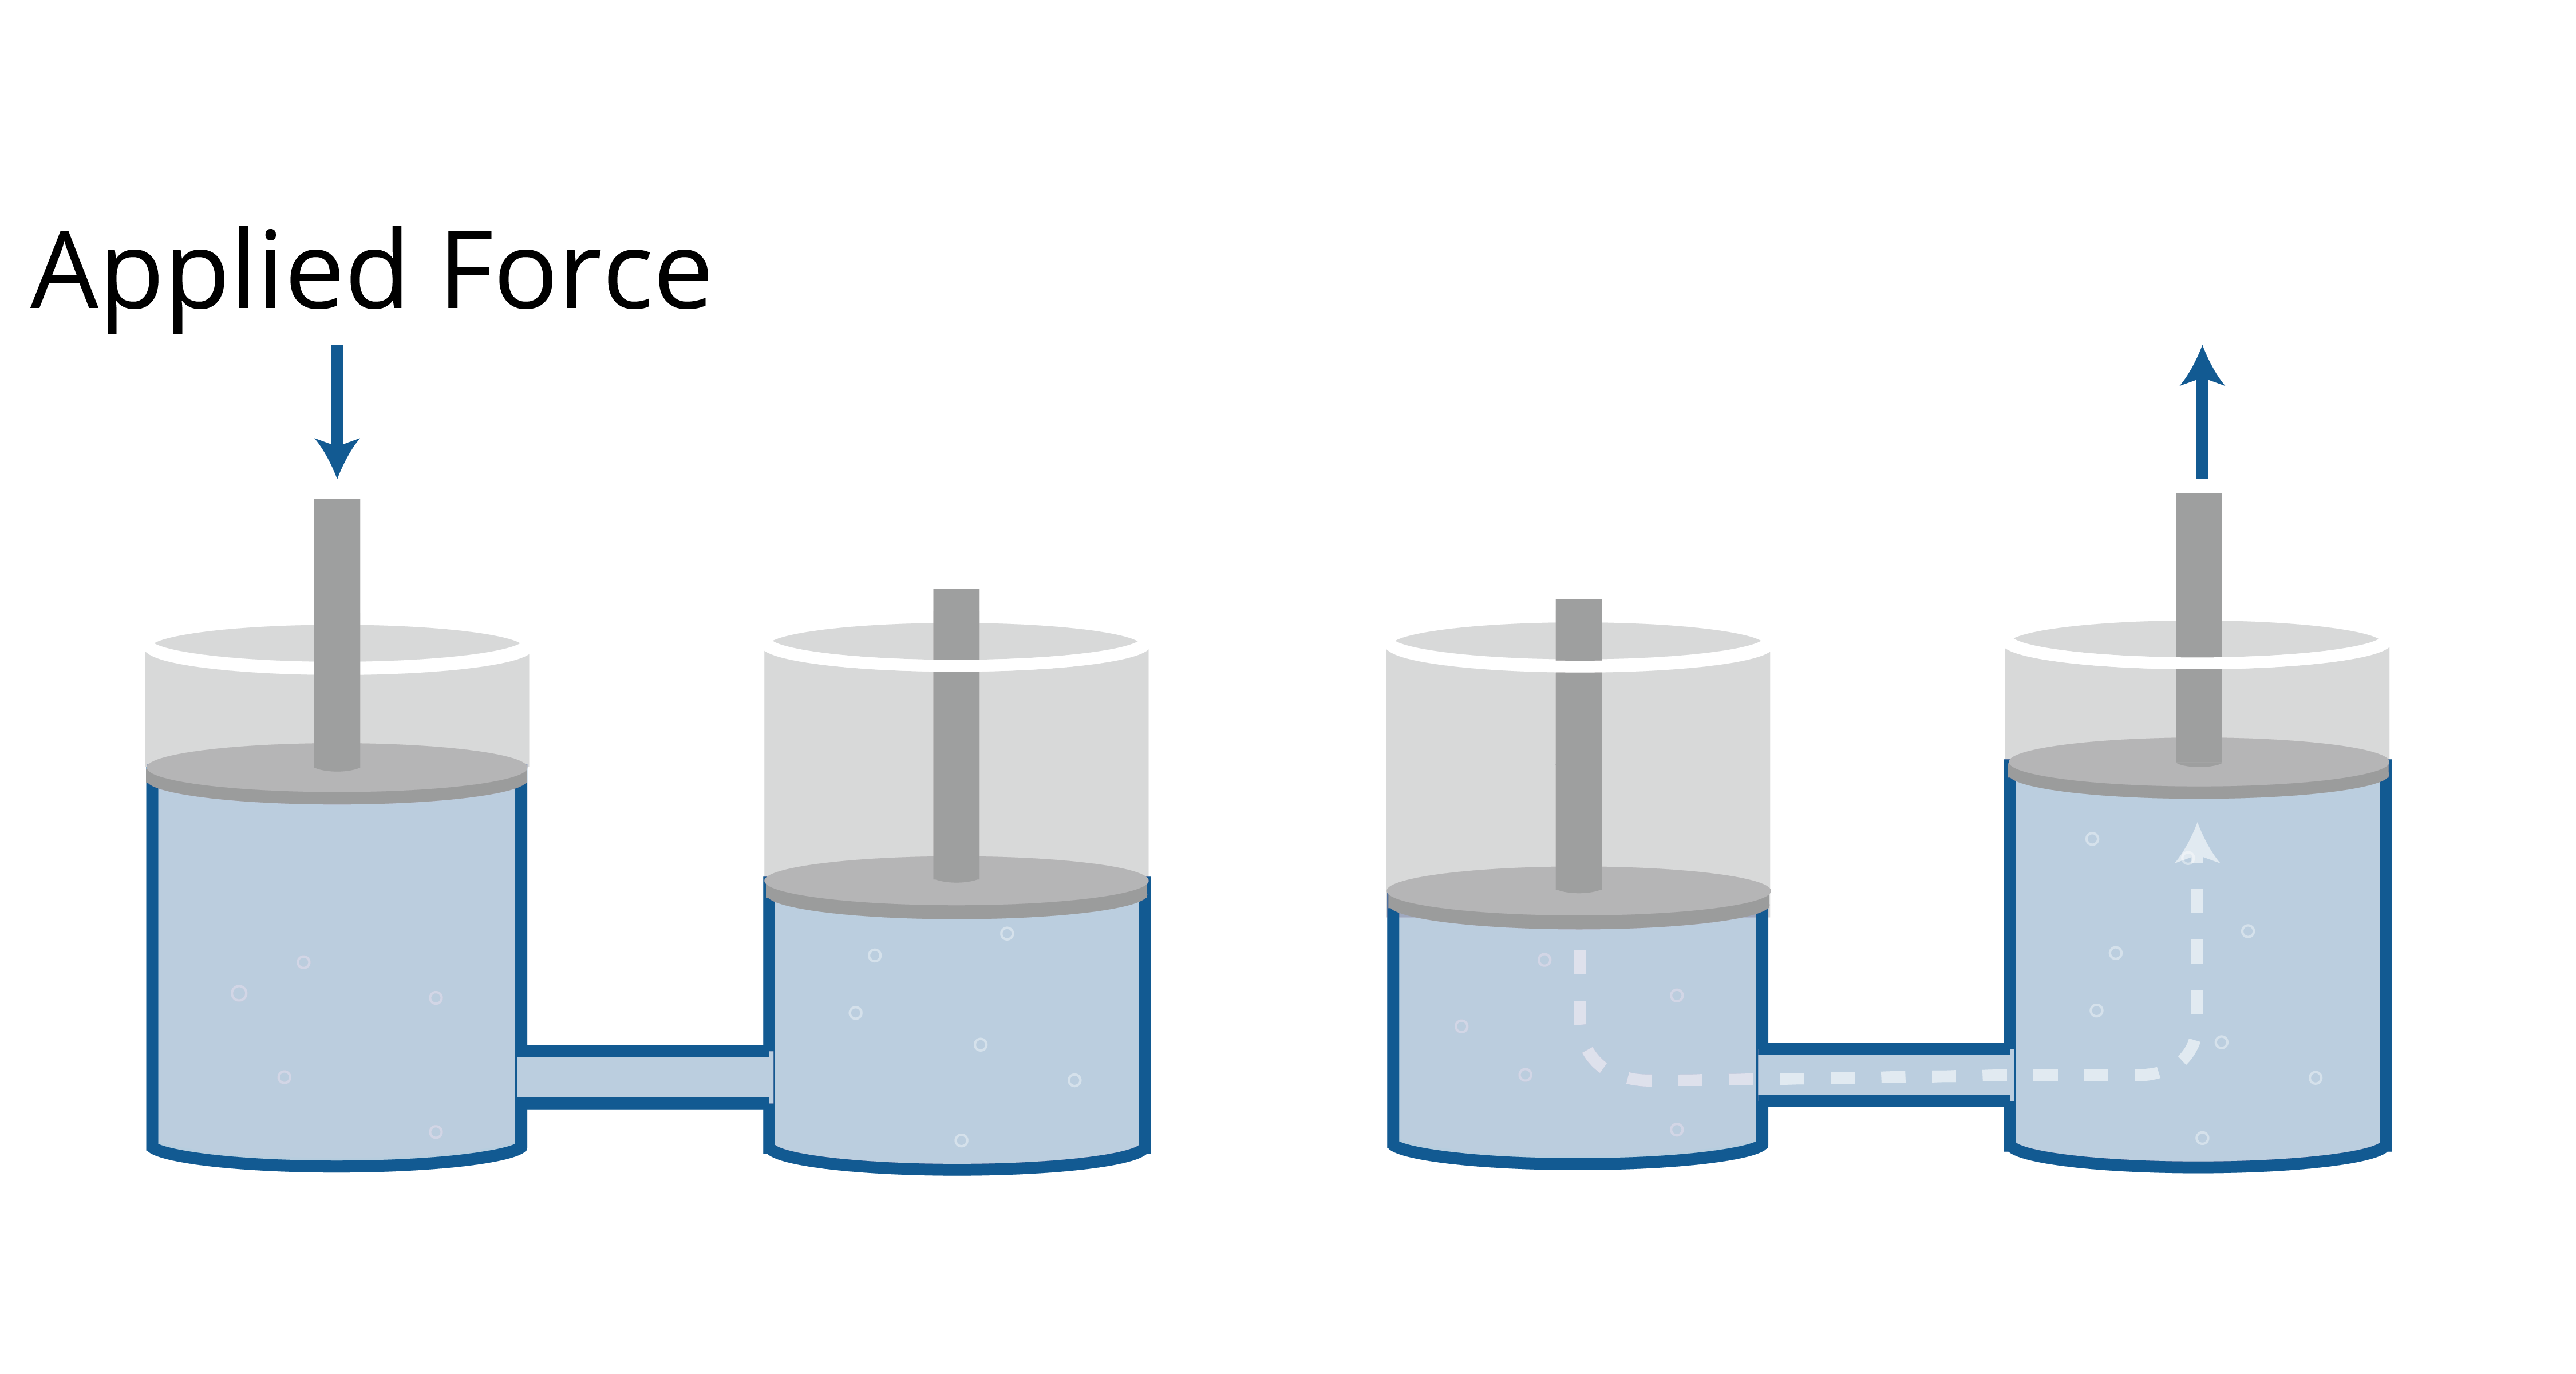
\includegraphics[width=\textwidth]{hydraulicsNew.png}

The pressure in the fluid is typically measured in pascals (Pa), which is equivalent to \(N / m^2\). We will use pascals for this calculation.

To calculate the pressure you create, divide the force applied by the area of the piston head. To determine the force on the other piston, multiply the pressure by the area of the second piston.

\begin{Exercise}[title={Hydraulics}, label=hydraulics]
Your car has disc brakes. When you apply 2,500,000 pascals of pressure to the brake fluid, the car stops quickly. As the car designer, you want this to require only 12 newtons of force from the driver's foot.

What should the radius of the master cylinder (the piston the driver pushes) be?
\end{Exercise}
\begin{Answer}[ref=hydraulics]
We are solving for the radius \( r \) of the piston. The area of the piston is \( \pi r^2 \), so the pressure is:

\[
\text{Pressure} = \frac{12}{\pi r^2}
\]

Setting the pressure equal to 2,500,000 pascals:

\[
2,500,000 = \frac{12}{\pi r^2}
\]

Solving for \( r \), we find:

\[
r = \sqrt{\frac{12}{\pi \times 2.5 \times 10^6}} \approx 0.00124 \text{ meters}.
\]
\end{Answer}

\graphicspath{{../../Chapters/buoyancy/en_US}}
\chapter{Buoyancy}

The word buoyancy probably brings to mind images of floating in water. Before we dive in, let's zoom out for a better understanding of everything buoyancy entails. You may be thinking: I want to be a computer programmer, why do I need to know about buoyancy? You might be surprised! This topic is much bigger than it seems at first glance. 

Buoyancy concerns the ways in which liquids and gasses interact with gravity. The concept of buoyancy is connected to fundamental concepts about how the universe works. The \newterm{buoyant force}, as it is known in engineering, is an important concept that has wide ranging applications. A big part of engineering is moving stuff around, and understanding buoyancy helps us solve problems where we need to move things in and through fluids. Even if you don't have plans to build a robotic submarine, these are incredibly useful ideas to be familiar with. We will start exploring the topic with familiar scenarios around boats and water.

When you put a boat into water, it will sink into the water until
the mass of the water it displaces is equal to the mass of the
boat. We think of this in terms of forces. Gravity pulls the mass of
the boat down; the \newterm{buoyant force} pushes the boat up. A boat
dropped into the water will bob up and down at first before reaching an
\newterm{equilibrium} where the two forces are equal.
% FIXME: Define displacement, and velocity. It is not defined in workbook one or this chapter (I think that would help) - Arjan
% ADD: Explain Action Reaction Pairs in previous chapter
% ADD: Archimedes principle

The buoyant force pushes things up, fighting against the force of
gravity. The force is equal to the weight of the fluid being
replaced. For example, a cubic meter of freshwater has a mass of
about 1000kg. If you submerge anything with a volume of one meter in
freshwater on earth, the buoyant force will be about 9800 newtons ($\text{mass} \times \ \text{gravity})$.

For some things, like a block of styrofoam, this buoyant force will be
sufficient to carry it to the surface. Once it reaches the surface, it
will continue to rise (displacing less water) until the mass of the
water it displaces is equal to its mass. And then we say ``It floats!''

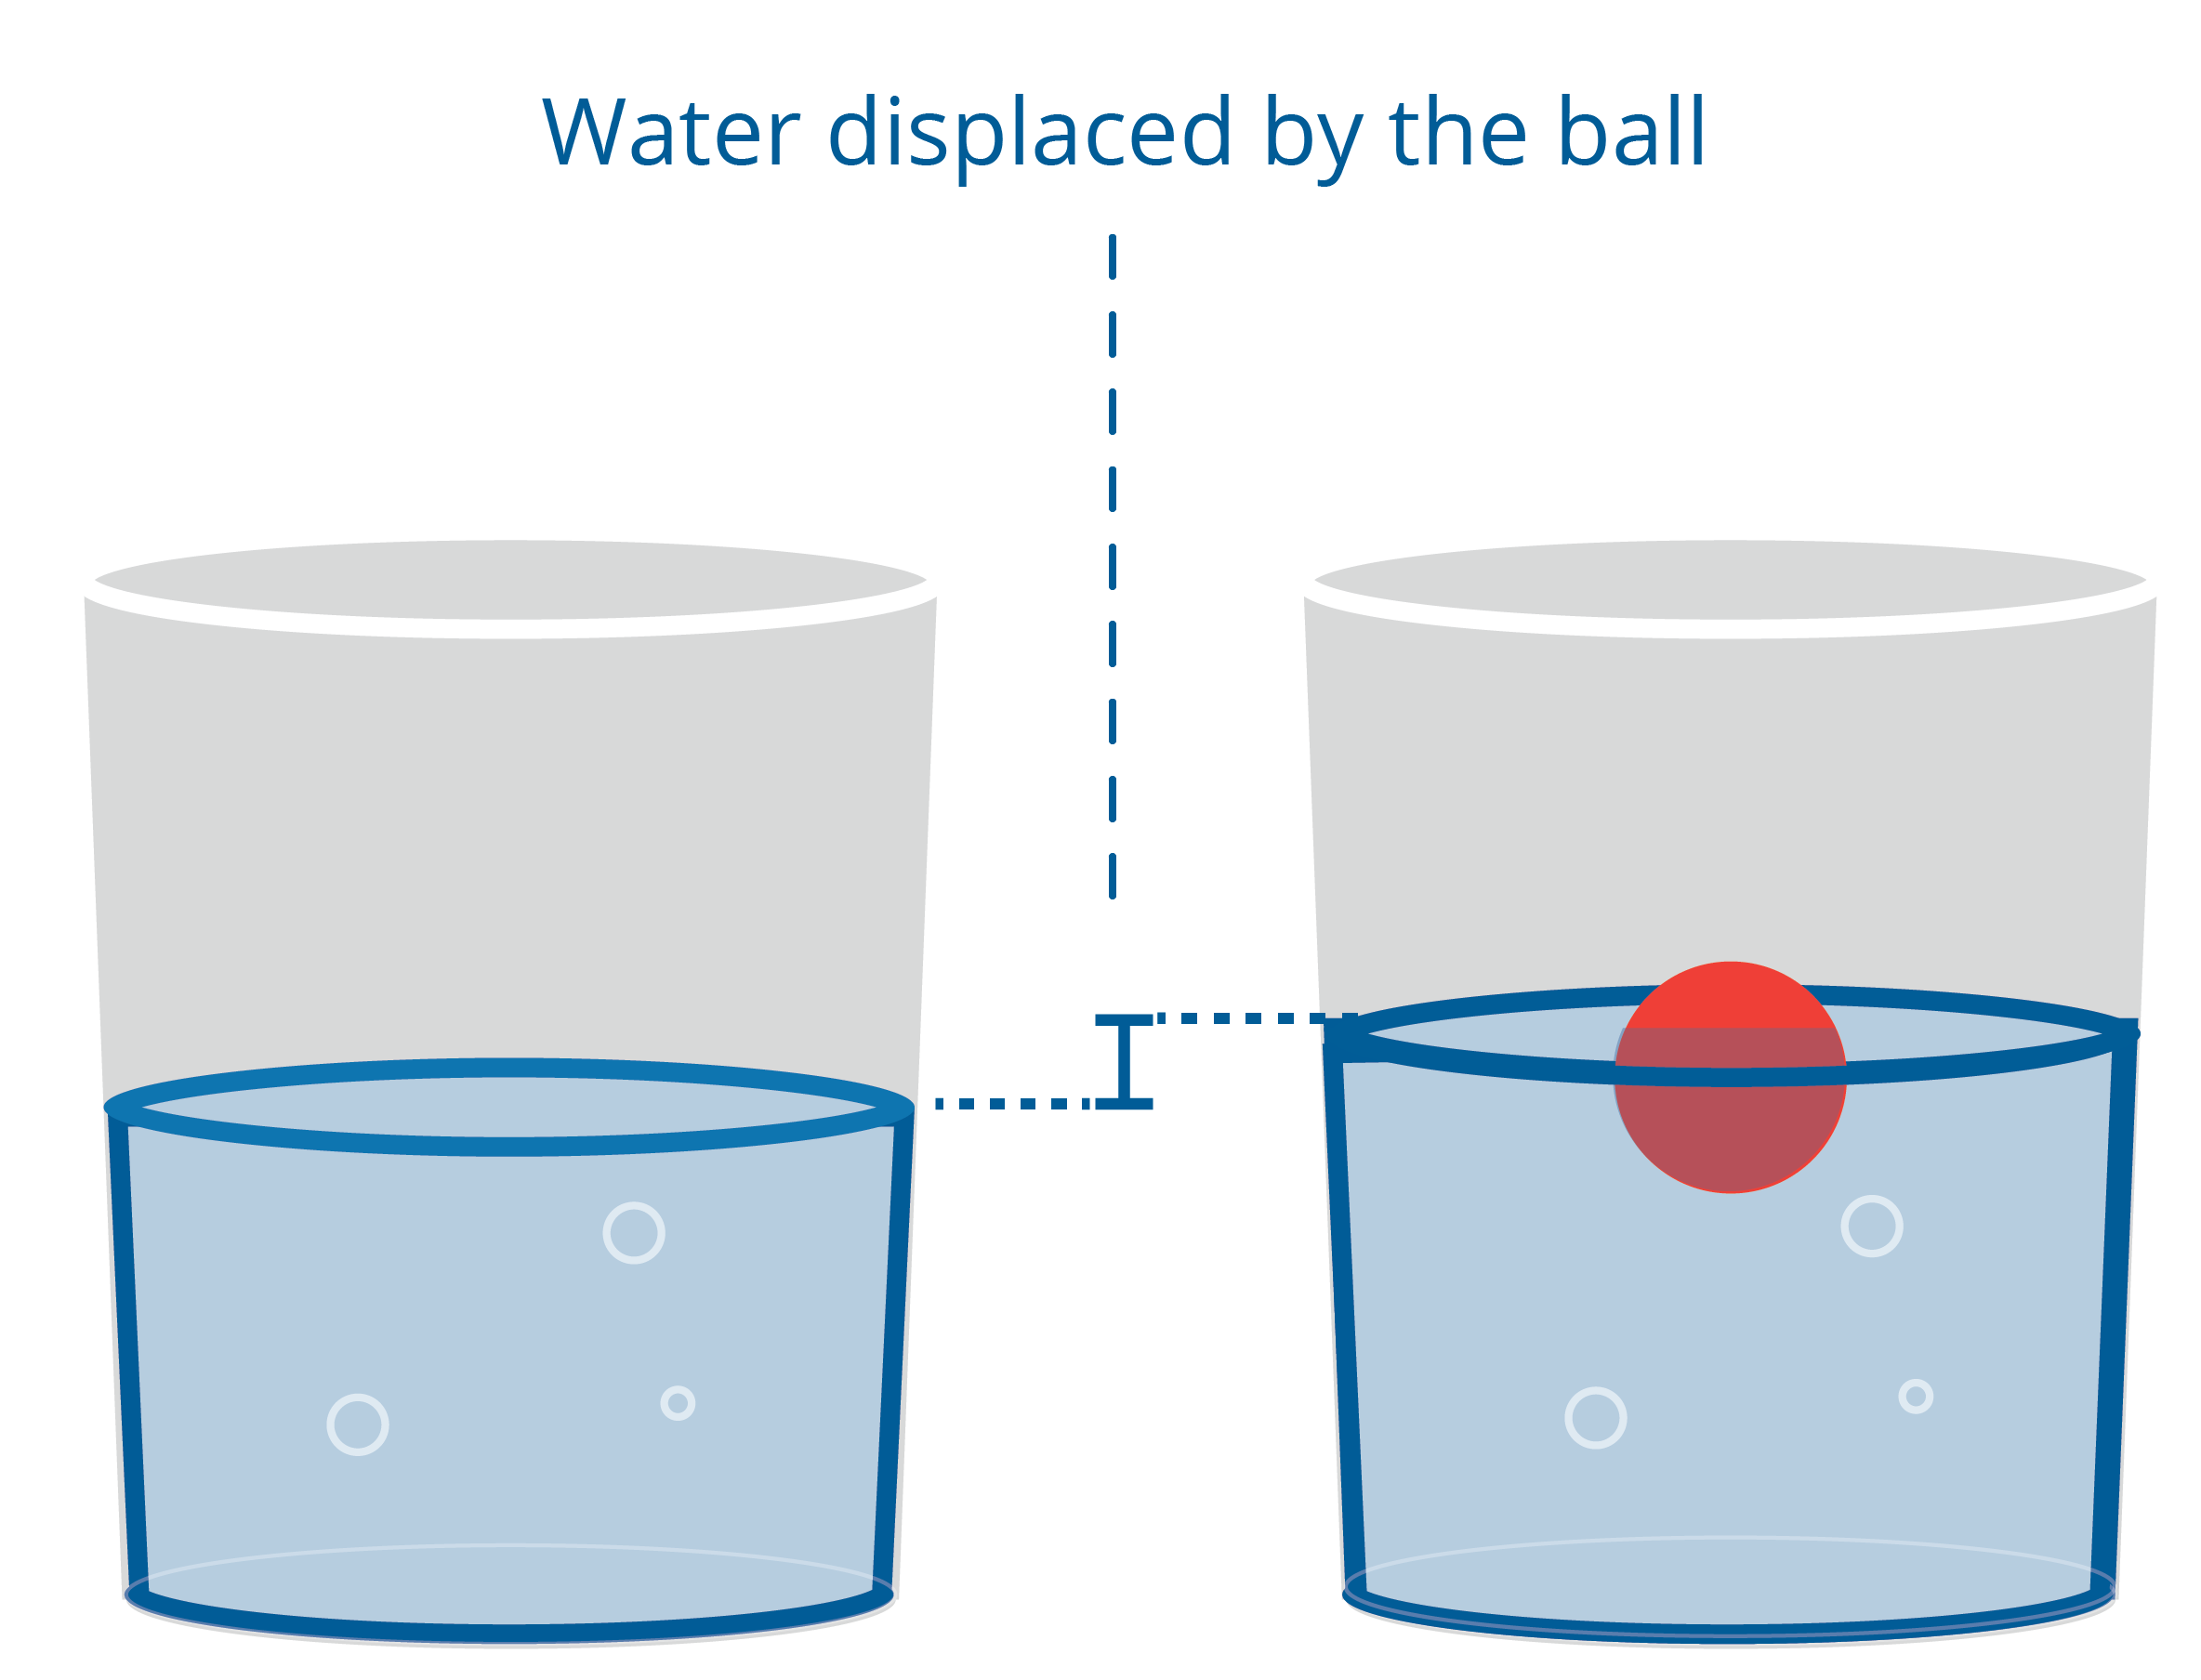
\includegraphics[width=.6\textwidth]{waterDisplacement.png}

For some things, like a block of lead, the buoyant force is not
 sufficient to lift it to the surface, and then we say ``It sinks!''

This is why a helium balloon floats through the air. The air
that it displaces weighs more than the balloon and the helium itself. (It is easy to forget that air has a mass, but it does.)

\begin{Exercise}[title={Buoyancy}, label=buoyancy]
  You have an aluminum box that has a heavy base, so it will always
  float upright. The box and its contents weigh 10 kg. Its base is 0.3 m x 0.4 m. It is 1m tall.

  When you drop it into freshwater ($1000 kg/m^3$), how far will it sink
  before it reaches equilibrium?\index{equilibrium}

\end{Exercise}
\begin{Answer}[ref=buoyancy]
  Equilibrium will be achieved when the box has displaced 10 kg of water. In other words, when it has displaced $0.01$ cubic meters.

  The area of the base of the box is 0.12 square meters. So if the
  box sinks $x$ meters into the water it will displace $0.12 x$ cubic
  meters.

  Thus at equilibrium $x = \frac{0.01}{0.12} \approx 0.083$ m. So
  the box will sink 8.3 cm into the water before reaching equilibrium.
\end{Answer}

\section{The Mechanism of Buoyancy: Pressure}

As you dive down in the ocean, you will experience greater and
greater pressure from the water. And if you take a balloon with you, you
will gradually see it get smaller as the water pressure compresses the
air in the balloon.

Let's say you are 3 meters below the surface of the water. What is the
pressure in Pascals (newtons per square meter)? You can think of the
water as a column of water crushing down upon you. The pressure over
a square meter is the weight of 3 cubic meters of water pressing down.

$$p = (3)(1000)(9.8) = 29,400 \text{ Pa }$$

This is called \newterm{hydrostatic pressure}. The general rule for
hydrostatic pressure in Pascals $p$ is

$p = d g h$

where $d$ is the density of the fluid
in kg per cubic meter, $g$ is the acceleration due to gravity in
$m/s^2$, and $h$ is the height of the column of fluid above you.

So where does buoyant force come from? Basically, the pressure pushing up on the
deepest part of the object is higher than the pressure pushing down on
the shallowest part of the object. That is where bouyancy comes from.

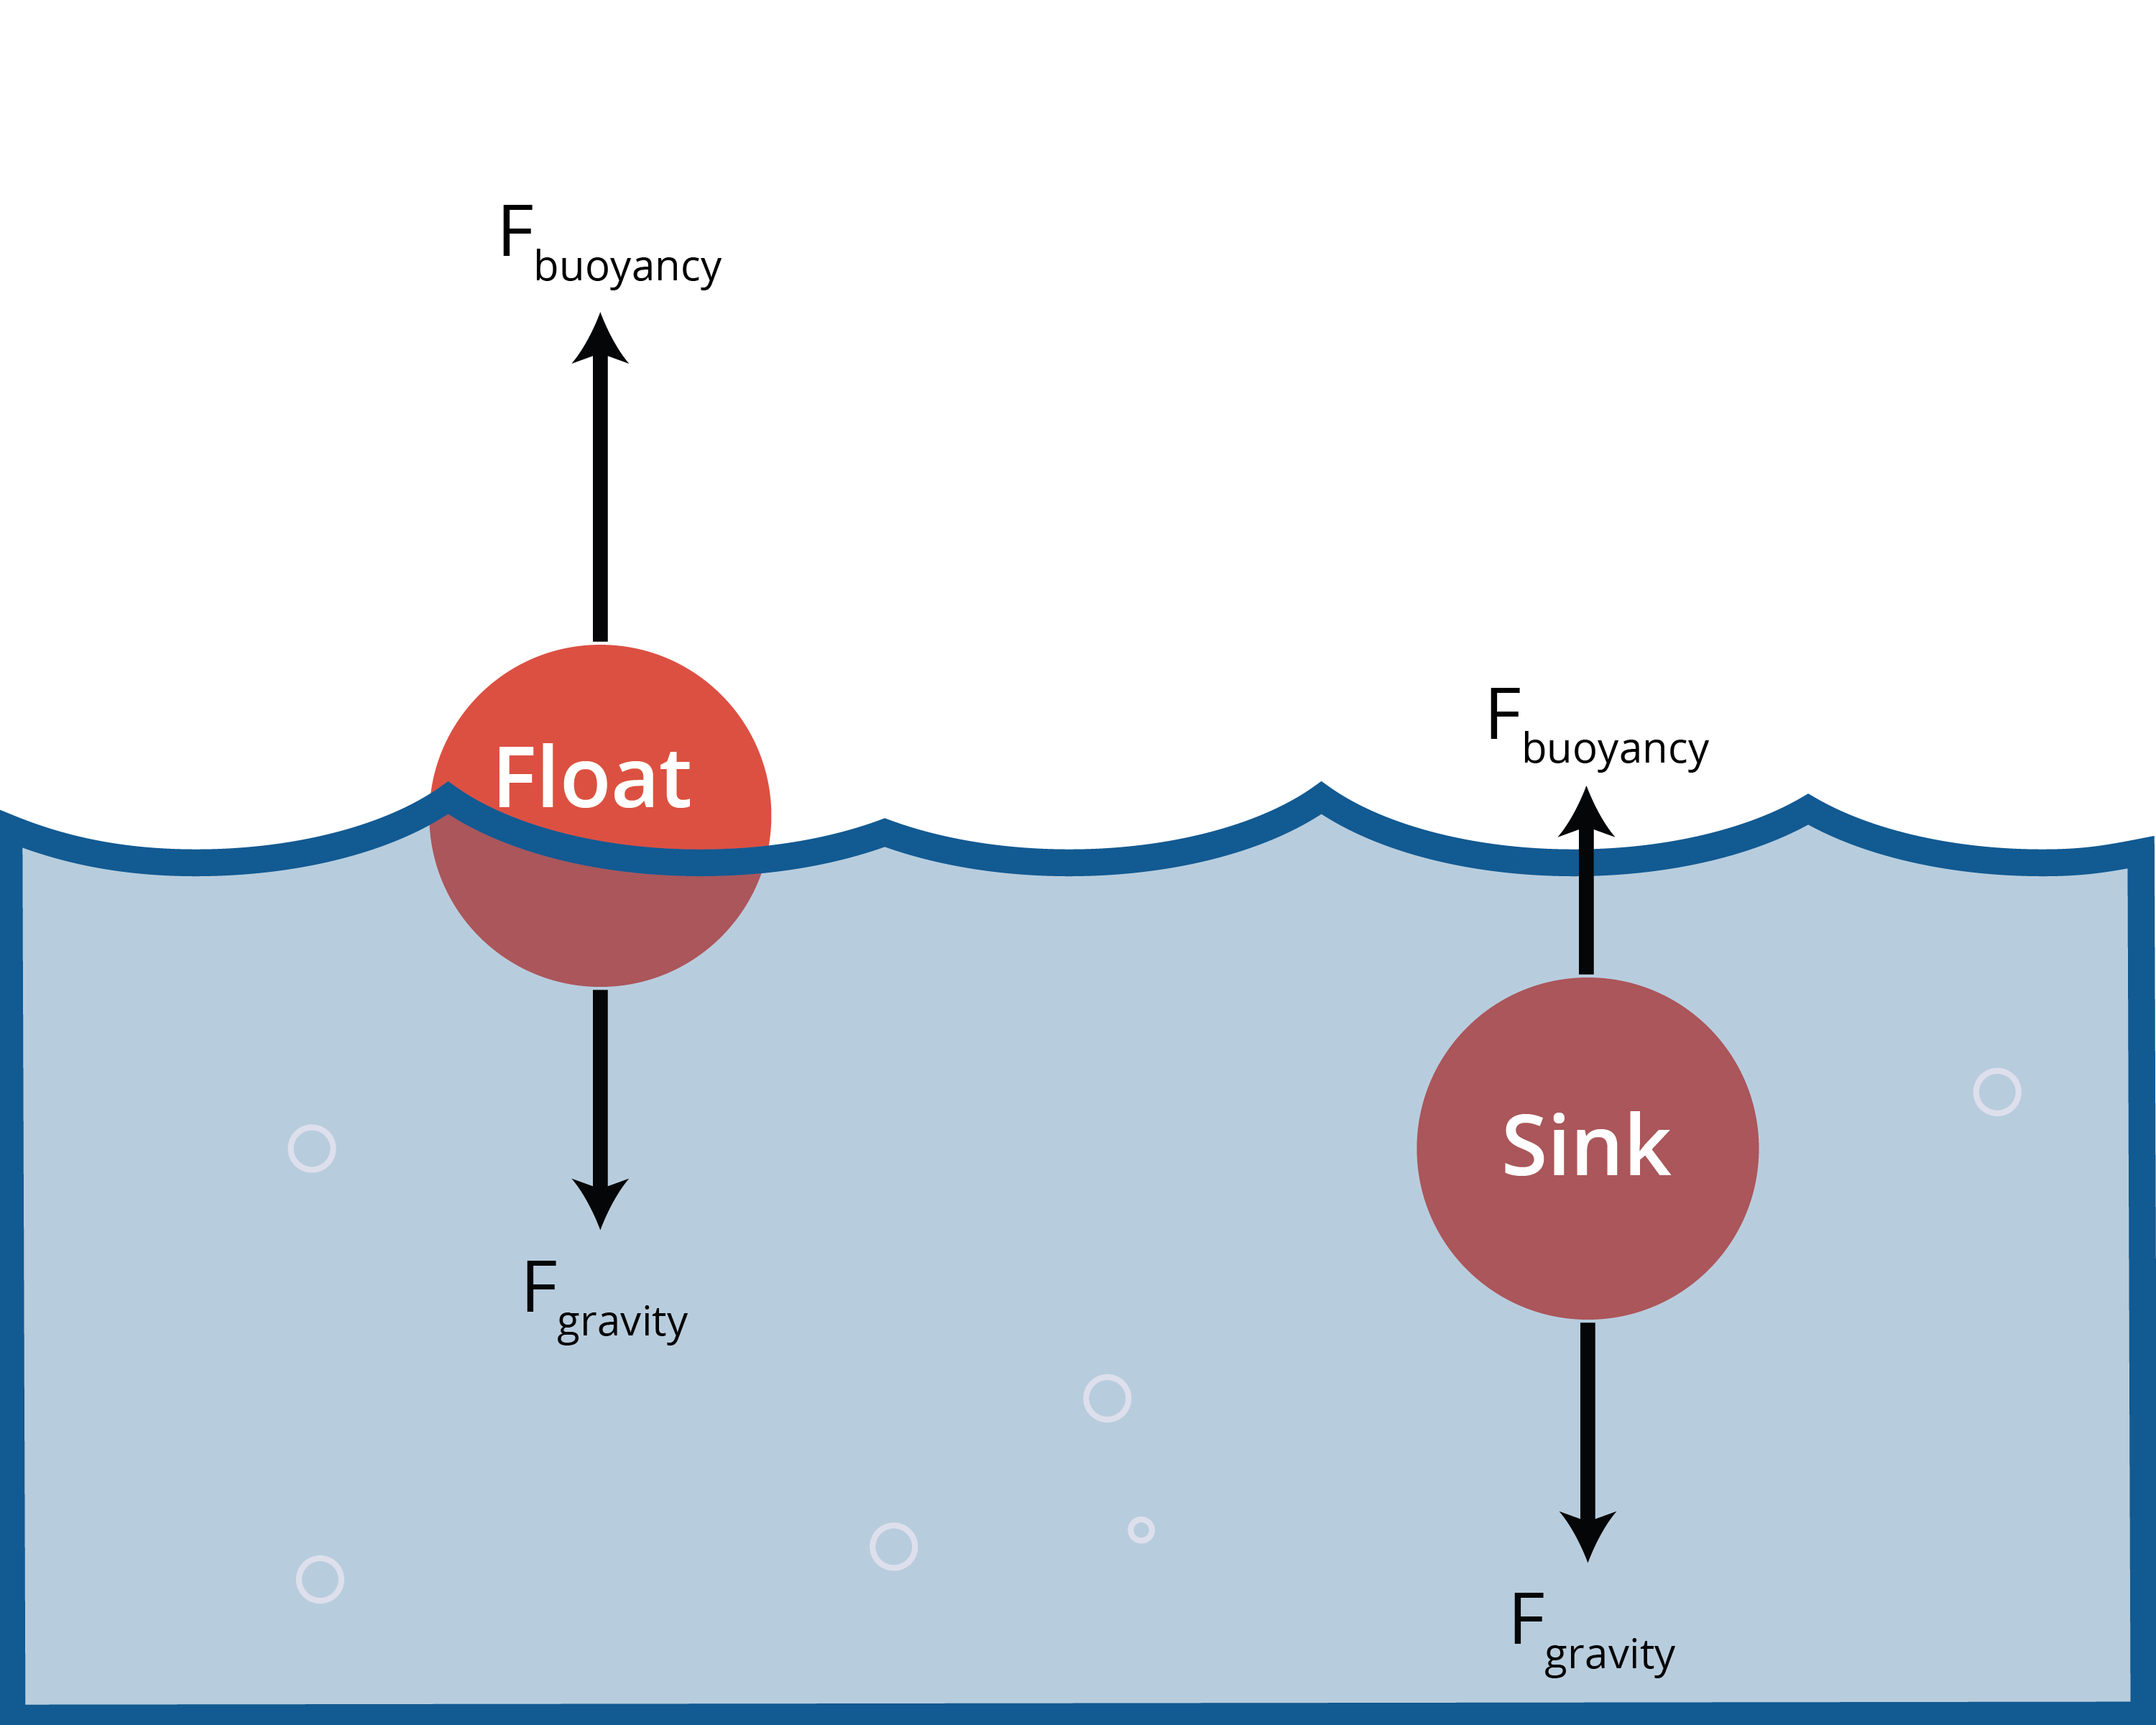
\includegraphics[width=.6\textwidth]{buoyancy.png}

\begin{Exercise}[title={Hydrostatic Pressure}, label=mars_pressure]

  You dive into a tank of olive oil on Mars. How much more
  hydrostatic pressure does your body experience at 5 meters deep than
  it did at the surface?

  The density of olive oil is about 900 kg per square meter. The
  acceleration due to gravity on Mars is 3.721 $m/s^2$.

\end{Exercise}
\begin{Answer}[ref=mars_pressure]
$$p = d g h = (900)(3.721)(5) = 16,744.5 \text{ Pa}$$
\end{Answer}

\section{The Mechanism of Buoyancy: Density}
Keep in mind that although the pressure is increasing as you go deeper, the
buoyant force will \emph{not increase}, because the buoyant force is always equal
to the weight of the fluid that is displaced, regardless whether that is 1
meter or 100 meters underwater.

Due to the added minerals, saltwater is denser than freshwater. This causes objects to float
better in the sea than they do in a river. Lipids, like fats and
oils, are less dense than water, allowing them to float on top of a glass of water.
When you're facing a grease fire, you're told not to put water on it. That's because
the water sinks below the grease, then boils, throwing burning grease everywhere.

\graphicspath{{../../Chapters/heat/en_US}}
\chapter{Heat}

All mass in the universe has heat, whether you're looking at a block of dry ice (frozen $CO_2$, $-78.5^\circ$ C)
or the surface of the sun ($5,600^\circ$ C). As long as the mass is above absolute zero --- the coldest possible
temperature in the universe --- there is some amount of heat in it.

\section{How Heat Works}

As you heat up an object, you are imparting energy into it. Where does this energy go? The atoms take this energy
and they begin to move, vibrating and bumping into each other, causing the heat to spread throughout. Everytime the
atoms collide and bounce off of each other, they emit a tiny amount of energy as light. In most cases, that light is
in the infrared spectrum, but in extreme cases can be visible, such as with molten lava or hot metal.

As objects interact, they either put heat into colder objects or take heat from warmer objects. That's what allows you to heat up
anything in the first place. The hot air from a stove or bunsen burner interacts with the pan or test tube you're heating,
passing the air's heat on. How could you model this?

\section{Specific Heat Capacity}

If you are heating something, the amount of energy you need to
transfer to it depends on three things: the mass of the thing you are
heating, the amount of temperature change you want, and the
\textit{specific heat capacity} of that substance.\index{specific heat capacity}

\begin{mdframed}[style=important, frametitle={Energy in Heat Transfer}]

  The energy moved in a heat transfer is given by

  $$E = m c \Delta_T$$

  where $m$ is the mass, $\Delta_T$ is the change in temperature, and
  $c$ is the specific heat capacity of the substance.
% ADD: q=mcat

  (Note that this
  assumes there isn't a phase change. For example, this formula works nicely on
  warming liquid water, but it gets more complicated if you warm the
  water past its boiling point.)

\end{mdframed}

Can we guess the specific heat capacity of a substance? It is very,
very difficult to guess the specific heat of a substance, so we determine
it by experimentation.

For example, it takes 0.9 joules to raise
the temperature of solid aluminum one degree Celsius. So we say ``The
specific heat capacity of aluminum is 0.9 J/g $^\circ$C.''

The specific heat capacity of liquid water is about 4.2 J/g $^\circ$C.

Let's say you put a 1 kg aluminum pan that is $80^\circ$ C into
3 liters of water that is $20^\circ$ C. Energy, in the form of heat,
will be transferred from the pan to the water until they are at the same
temperature. (We call this ``thermal equilibrium.'')\index{thermal equilibrium}

What will the temperature of the water be?

To answer this question, the amount of energy given off by the
pan must equal the amount of energy absorbed by the water. They also
need to be the same temperature at the end. Let $T$ be the final
temperature of both.

3 liters of water weighs 3,000 grams, so the
change in energy in the water will be:

$$E_W = m c \Delta_T = (3000)(4.2)(T - 20) = 12600T - 252000 \text{ joules}$$

The pan weighs 1000 grams, so the change in energy in the pan will be::

$$E_P = m c \Delta_T = (1000)(0.9)(T - 80) = 900T - 72000 \text{ joules}$$

The total energy stays the same, so $E_W + E_P = 0$. This means you need to solve

$$(12600T - 252000) + (900T - 72000) = 0$$

And find that the temperature at equilibrium will be

$$T = 24^\circ \text{C}$$

\begin{Exercise}[title={Thermal Equilibrium}, label=thermal_equilibrium]

Just as you put the aluminium pan in the water as described above,
someone also puts a 1.2 kg block of copper cooled to 10 $^\circ$ C.
The specific heat of solid copper is about 0.4 J/g $^\circ$C.

What is the new temperature at equilibrium?

\end{Exercise}
\begin{Answer}[ref=thermal_equilibrium]

  $$E_C = (1200)(0.4)(T - 10) = 480T - 4800$$

Total energy stays constant:

$$0 = (12600T - 252000) + (900T - 72000) + (480T - 4800)$$

Solving for $T$ gets you $T = 23.52^\circ$ C.

\end{Answer}

\section{Getting to Equilibrium}

When two objects with different temperatures are touching, the speed
at which they exchange heat is proportional to the differences in
their temperatures. As their temperatures get closer together,
the heat exchange slows down.
% ADD: explain which object, water or metal has a greater tempature change

In our example, the pan and the water will get close to equilibrium
quickly, but they may never actually reach equilibrium.

\begin{tikzpicture}
    \begin{axis}[
        xmin=0,xmax=4.25,
        ymin=15,ymax=85,
        axis x line=middle,
        axis y line=middle,
        axis line style=<->,
        xlabel={minutes},
        ylabel={degrees celsius},
        ]
        \addplot[no marks,sdkblue] expression[domain=0:4,samples=100]{24 + 56 * pow(2,-1.5 * x)} node[above, xshift=-1cm, yshift=0.1cm]{Pan};
        \addplot[no marks,sdkblue] expression[domain=0:4,samples=100]{24 - 4 * pow(2,-0.8 * x)} node[below, xshift=-2.5cm]{Water};
        \addplot[no marks,dashed,gray] coordinates {(0,24)(6,24)} node[above, xshift=-8cm]{equilibrium};
    \end{axis}
\end{tikzpicture}

\begin{Exercise}[title={Cooling Your Coffee}, label=cool_coffee]

  You have been given a ridiculously hot cup of coffee and a small pitcher of chilled milk.

  You need to start chugging your coffee in three minutes, and you want it as cool as possible at that time. When should you add the milk to the coffee?

\end{Exercise}
\begin{Answer}[ref=cool_coffee]

  During the 3 minutes, you want the coffee to give off as much of its
  heat as possible, so you want to maximize the difference between the
  temperature of the coffee and the temperature of the room around
  it.

  You wait until the last moment to put the milk in.

\end{Answer}

\section{Specific Heat Capacity Details}

For any given substance, the specific heat capacity often changes a
great deal when the substance changes state. For example, ice is 2.1 J/g
$^\circ$C, whereas liquid water is 4.2 J/g$^\circ$C.

Even within a given state, the specific heat capacity varies a bit
based on the temperature and pressure. If you are trying to do these
sorts of calculations with great accuracy, you will want to find the
specific heat capacity that matches your situation. For example, I
might look for the specific heat capacity for water at $22^\circ$C at
1 atmosphere of pressure (atm).

\graphicspath{{../../Chapters/biases1/en_US}}
\chapter{Cognitivie Biases 1}


Our brains were designed over millions of years by the evolutionary
process. The resulting mind is an amazing and powerful tool, but it is
not flawless. The human brain has tendencies (or biases) that nudge us
toward bad judgment and poor decisions.

It would be irresponsible for us to teach you powerful ideas without
also teaching you about these cognitive biases. There are about 50
that you should know about, so we will have a few that introduce them.

\section{Fundamental Attribution Error}

You tend to attribute
the mistakes of another person to their character, but attribute your
own mistakes to the situation.

Let's say you are at lunch and someone asks you ``Why was Larry late
for class ?''  You are likely to say ``Larry is lazy
and disorganized.''

If someone asks you ``Why were you late for class last week?''  You
are likely to say, ``I don't remember; The class before it must have
run long.''

The solution? Cut people some slack. You probably don't know the whole
story, so assume that their character is as strong as yours.

Or maybe you also need to hold yourself to a higher standard? Do you find
yourself frequently rationalizing your bad judgment, lateness, or
rudeness?  This could be an opportunity for you to become a better
person whose character is stronger regardless of the situation.

\section{Self-Serving Bias}

\newterm{Self-serving bias} is when you blame the situation for your
failures, but attribute your successes to your strengths.

For example, when asked ``Why did you lose the match?'' you are likely
to answer ``The referee wasn't fair.''  When you are asked ``Why did
you win the match?'' you are likely to answer ``Because I have been
training for weeks, and I was very focused.''

This bias tends to make us feel better about ourselves, but it makes it
difficult for us to be objective about our strengths and weaknesses.

\section{In-group favoritism}

\newterm{In-group favoritism}: We tend to favor people who are in
a group with us over people who are not in groups with us.

When asked ``Who is the better goalie, Ted or John?''

If Ted is a Star Trek fan like you, you are likely to think he is also
a good goalie.

As you might imagine, this unconscious tendency is the source of a lot
of subtle discrimination based on race, gender, age, and religion.

\section{The Bandwagon Effect and Groupthink}

\newterm{The bandwagon effect} is our tendency to believe the same
things that the people around us believe. This is how fads spread so
quickly: one person buys in, and then the people they know have a
strong tencdency to buy in as well.

\newterm{Groupthink} is similar: To create harmony with the
people around us, we go along with things we disagree with.

It takes a lot of perspective to recognize when those around us are
wrong. And it takes even more courage to disagree with them.

\section{The Curse of Knowledge}

Once you know something, you tend to assume everyone else knows it too.

This is why teaching is sometimes difficult: a teacher will assume
that everyone in the audience already knows the same things the
teacher knows.

Also, when we learn that a friend doesn't know something that we know,
we are often very surprised.  This surprise can sometimes manifest as
hurtful behavior.

When I find a gap in a friend's knowledge, I try to remind myself that
the friend certainly knows many things that I don't.  I also try to
imagine how it would feel if they teased me for my ignorance.

\section{False Consensus}

You tend to believe that more people agree with us than is actually
the case. For example, if you are a member of a particular religion,
you tend to overestimate the percentage of people in the world who are
members of that religion.

When people vote in elections, they are often surprised when their
preferred candidate loses. ``Everyone, and I mean EVERYONE, voted for
Smith!'' they yell.  ``There must have been a mistake in counting the
votes.''

\section{The Spotlight Effect}

You tend to overestimate how much other people are paying attention to
your behavior and appearance.

Think of six people that you talked to today.  Can you even remember what
shoes most of them were wearing? Do you care? Do you think any of them
remember which shoes you wore today?

There is an old saying ``You would worry a lot less about how people
think of you if you realized how rarely they do.''

\section{The Dunning-Kruger Effect}

The less you know, the more confident you are.

When a person doesn't know all the nuance and context in which a question is
asked, the question seems simple. Thus the person tends to be confident in
their answer.  As they learn more about the complexity of the space in
which the question lives, they often realize the answer is not nearly so
obvious.

For example, a lot of people will confidently proclaim ``Taxes are too
high! We need to lower taxes.''  An economist who has studied
government budgets, deficits, history, and monetary policy, might say
something like ``Maybe taxes \emph{are} too high.  Or maybe they are
too low. Or maybe we are taxing the wrong things. It is a 
complex question.''

When I am talking with people about a particular topic, I do my best
to defer to the person in the conversation who I think has the most
knowledge in the area. If I disagree with the person, I try to figure
out why our opinions are different.

Similarly, you should assume that any opinion that is voiced in an
internet discussion is wildly over-simplified.  If you really care
about the subject, read a book by a respected expert. Yes, a whole
book -- there are few interesting topics that can be legitimately
explained in less than 100 pages.

\section{Confirmation Bias}

You tend to find and remember information that supports
beliefs you already have. You tend to avoid and dismiss information
that contradicts your beliefs.

If you believe that intelligent creatures have visited from other
planets, you will tend to look for data to support your beliefs. When
you find data that shows that it is just too far for any creature to
travel, you will try to find a reason why the data is incorrect.

Confirmation bias is one reason why people don't change their beliefs
more often.

Confirmation bias wrecks many, many studies. The person doing the
study often has a hypothesis that they believe and very much want to
prove true. It is very tempting to discard data that doesn't support
the hypothesis. Or maybe the person throws all the data away and experiments again and again until they get the result they want.

When you design an experiment, you must describe it explicitly before
you start. You must tell someone: ``If the hypothesis I love is
incorrect, the results will look like this.  If the hypothesis I love
is correct, the results will look like that. And if the results look
any other way, I have neither proved nor disproved the hypothesis.''

Once the experiment is underway, you must not change the plan and you
must not discard any data.

This is scientific integrity. You should demand it from yourself, and
you should expect it from others.

\section{Survivorship bias}

You will pay more attention to those that survived a process than
those who failed.

After looking at a lot of old houses, you might say ``In the 1880s,
they built great houses.'' However, you haven't seen the houses that
were built in the 1880s and didn't survive.  Which houses tended to
survive for a long time? Only the great houses -- you are
basing your opinion on a very skewed sample.


\graphicspath{{../../Chapters/friction/en_US}}
\chapter{Friction}

Imagine there is a large and heavy steel box resting in the middle of a floor, and you push it hard enough to get it moving. If you stop pushing, will it continue to glide gracefully across the floor? 

Probably not. Unless the floor is very slippery for some reason, the box will come to a halt immediately after you stop pushing. We would say that it is stopped by the force of \newterm{friction}. 

What is really happening? The kinetic energy of the box is being converted into heat 
between the bottom of the box and floor. As the bottom of the box and the floor get warmer, the speed of the box decreases.

The amount of friction is proportional to the force with which the box is pressing against the floor --- so you should expect a box that is twice as heavy to experience twice as much frictional force.

In other words, the frictional force is proportional to the normal force. On a level floor, the normal force is parallel and equal to the force of gravity acting on the box. On a slope, the normal force points perpendicular to the surface of the slope. We will be talking about sloped surfaces in a later chapter, so focus on level surfaces for now. 

(FIXME: picture here)

The amount of friction is also determined by the materials that are sliding against each other. For example, if the floor is ice, the frictional force will be less than if the floor is made of wood. Written mathmatically, we can express the force of friction as
$$F_{f} = \mu N$$

where $F_{f}$ is the force of friction, $N$ is the normal force (you may see written as $R \ , F_{n} \ , \text{or just} \ N$), and $\mu$ is a coefficient that depends on the materials in contact with each other.

If you are pushing the box with a force of $F$ and it is moving but neither accelerating nor decelerating, then the force you are applying is exactly balanced by the frictional force. If the box is pressing against the floor with a force of $N$, then we say the \newterm{coefficient of friction} is given by the ratio between the weight of the steel box and the floor:

$$\mu = \frac{F_{f}}{N}$$

\begin{Exercise}[title={Bicycle Stopping},  label=bike_stop]
  
You are riding your bicycle on a flat, horizontal at 11 meters per second when you suddenly slam on the brakes and lock up the wheels.  

You weigh 55 kg.   

When any piece of rubber is skidding across a dry road, the coefficient of friction will be about 0.7.

Answer the following questions: 

\begin{itemize}
\item How much kinetic energy do you have when you engage the brakes?
\item As you skid,  how much frictional force is decelerating you?
\item For how many meters will you slide?
\end{itemize}

\end{Exercise}
\begin{Answer}[ref=bike_stop]

Kinetic energy? $E = \frac{1}{2}mv^2 = (.5)(55)(11^2) = 3,327.5 \frac{kg m^2}{s^2} = 3,327.5$ joules.

Frictional force? $F = \mu N = (0.7)(55)(9.8) = 377.3$ newtons.

Distance?  $D = \frac{3,327.5}{377.3} \approx 8.8$ seconds. (found by using $W = F_f D$ and $W = \Delta E$)

\end{Answer}

Notice that the force of friction is not determined by how much of the tire is touching the ground. The coefficient of friction of the two materials and the normal force is all you need to compute the friction.
%ADD: Section about normal force?
\section{Static vs Kinetic Friction Coefficients}

Let's return to the box on the floor we discussed earlier. As you start to push it, it will sit still until your force is greater than the force of friction.   However, once it starts moving,  the force of friction seems to be less.

Between the two materials,  there are actually two different friction coefficients:

\begin{itemize}
\item Kinetic friction coefficient: The coefficient you use once the box is sliding against the floor.
\item Static friction coefficient: The coefficient you use to figure out how much force you need to get the box to start to move.
\end{itemize}

The kinetic friction coefficient is always less than the static friction coefficient:
\begin{itemize}
\item \textit{Kinetic}, $\mu_k$: For a car skidding on a dry road, the friction coefficient is about 0.7.  
\item \textit{Static}, $\mu_s$: When the car is parked with its brakes on, it has a friction coefficient of about 1.0.
\end{itemize}

\begin{Exercise}[title={Rocket Sled},  label=rocketsled1]
  
You are built a rocket sled with steel runners on a flat, level wooden floor. The sled weighs 50 kg and you weigh 55 kg.

Before you get on the sled,   you try pushing it around the floor. You find that you can get it to move from a
standstill if you push it with a force of 270 N.   Once it is moving,  you can keep it moving at the same speed using a force of 220 N.

\textbf{What are $\mu_s$ and $\mu_k$  of your sled's runners on your wooden floor?}

Next, you get on the sled and gradually increase the thrust of the rocket mounted on the sled until it starts to move. You then keep the thrust constant.

\textbf{How much force was the rocket exerting on you and the sled when it started to move?}

\textbf{How how fast do you accelerate now that the sled is moving?}

\end{Exercise}
\begin{Answer}[ref=rocketsled1]

The empty sled is pushing directly down on the floor with a force of $(50)(9.8) = 490$ N.

The force to overcome the static friction is:

$$270 = 490 \mu_s$$

Thus, $\mu_s = 0.551$

The force to match kinetic friction is:

$$220 = 490 \mu_k$$

Thus, $\mu_k = 0.449$

Once you are on the sled, it is pressing directly down on the floor with a force of $(50  + 55)(9.8) = 1,029$ N.

The force to overcome the static friction is:

$$F = (1,029)(0.551) = 567 \text{ N}$$

Once the sled is moving, friction is counteracting some of your force. How much?

$$F_f = (1,029)(0.449) = 462 \text{ N}$$

All of your acceleration is due to the remaining $567 - 492 = 75$ N.

We know that $F = ma$. In this case $F = 75$ N and $m = 105$ kg. So

$$a = \frac{75}{105} = 0.714 \text{ meters per second per second}$$

\end{Answer}

\section{Skidding and Anti-Lock Braking Systems}

When a car goes through a curve, the friction of the tire on the road is what changes the direction of the 
car's travel. Even though the wheel is turning, this is the static friction coefficient because the surface of the tire is not sliding across the road.

If you go into the curve too fast,  the tire may not have enough friction to turn the car.  In this case the car will start to slide sideways. Now the friction between the tire and road uses the kinetic coefficient. In other words, you have significantly less friction than you had before you started to skid.

When you are driving a car,  the force of friction that your tires create is your friend.  It lets you steer, accelerate, and stop.

In older cars,  if you would panicked  and slammed on the brakes,  you would probably lock up the wheels: they would stop turning suddenly.  And the surface of the tire would begin to slide across the pavement.  At that moment,  two problems occurred:
\begin{itemize}
\item You don't stop as quickly, because now the friction between your tires and the road is based on the kinetic friction coefficient instead of the static friction coefficient.
\item You can't steer the car. Steering only happens because the wheels are turning in a particular direction.
\end{itemize}

To prevent this problem, car companies developed the anti-lock brake system, or ABS.

FIXME: More here.

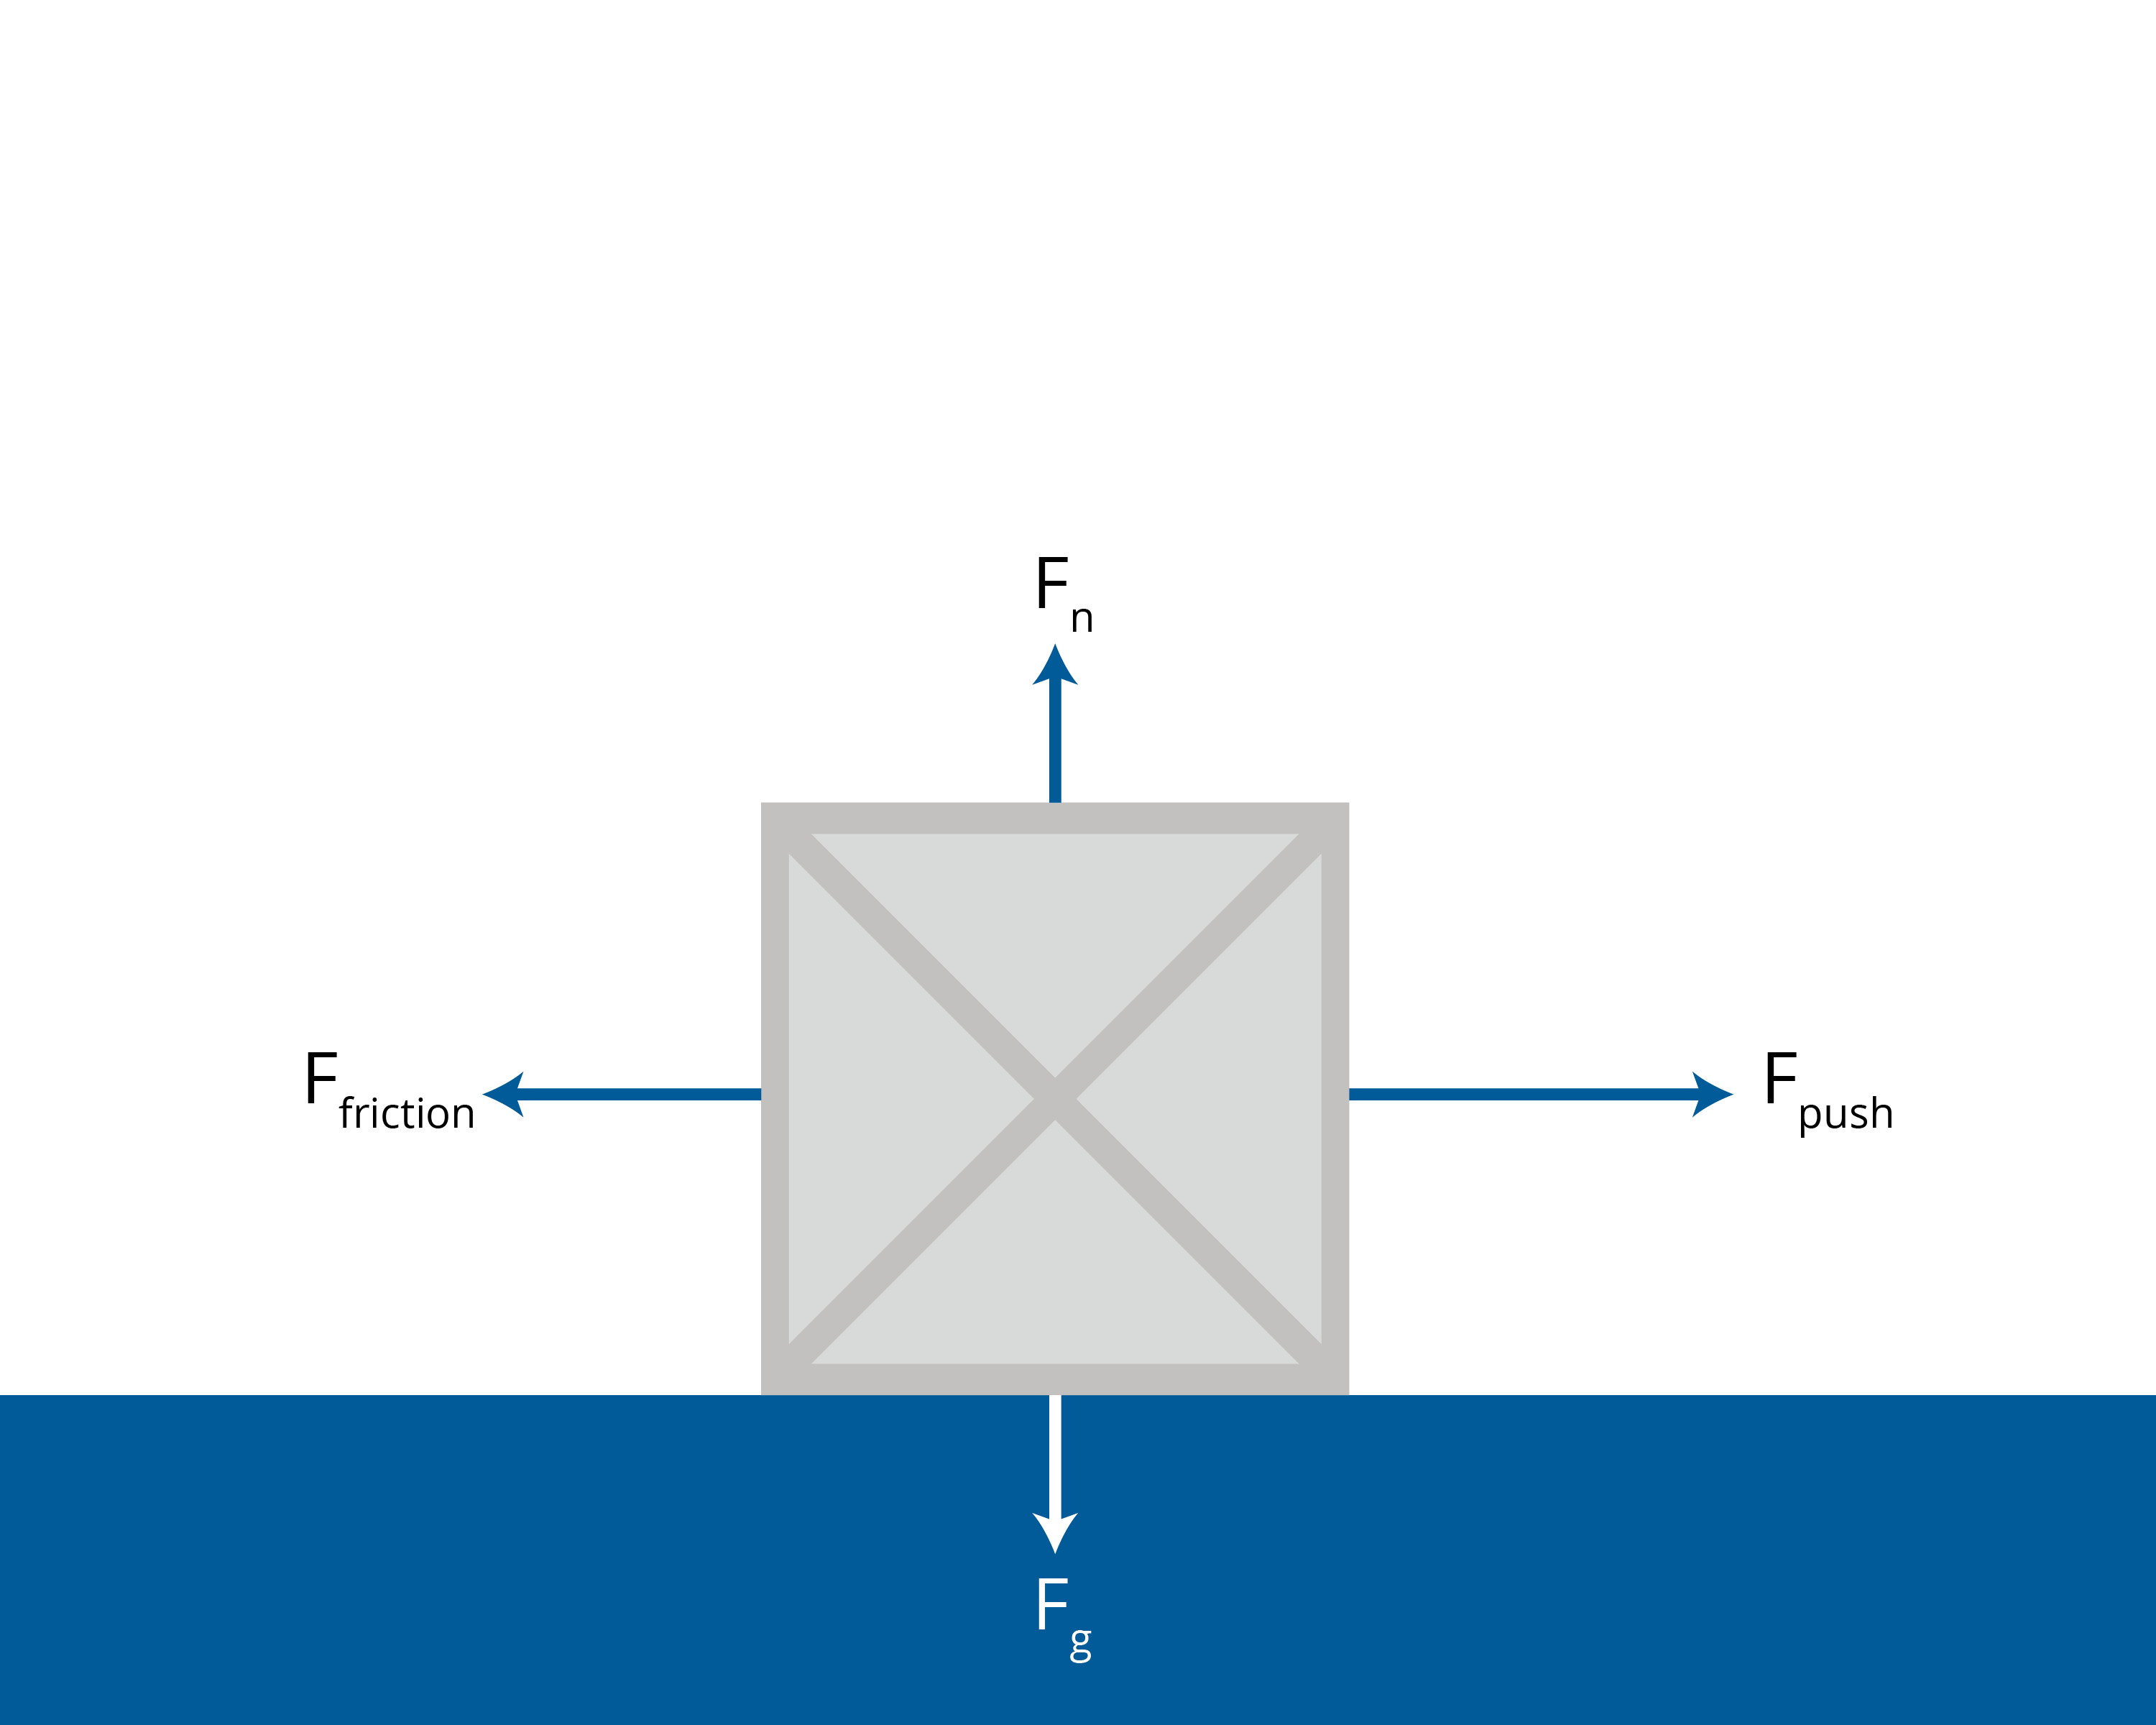
\includegraphics[width=0.75\textwidth]{friction-01.png}

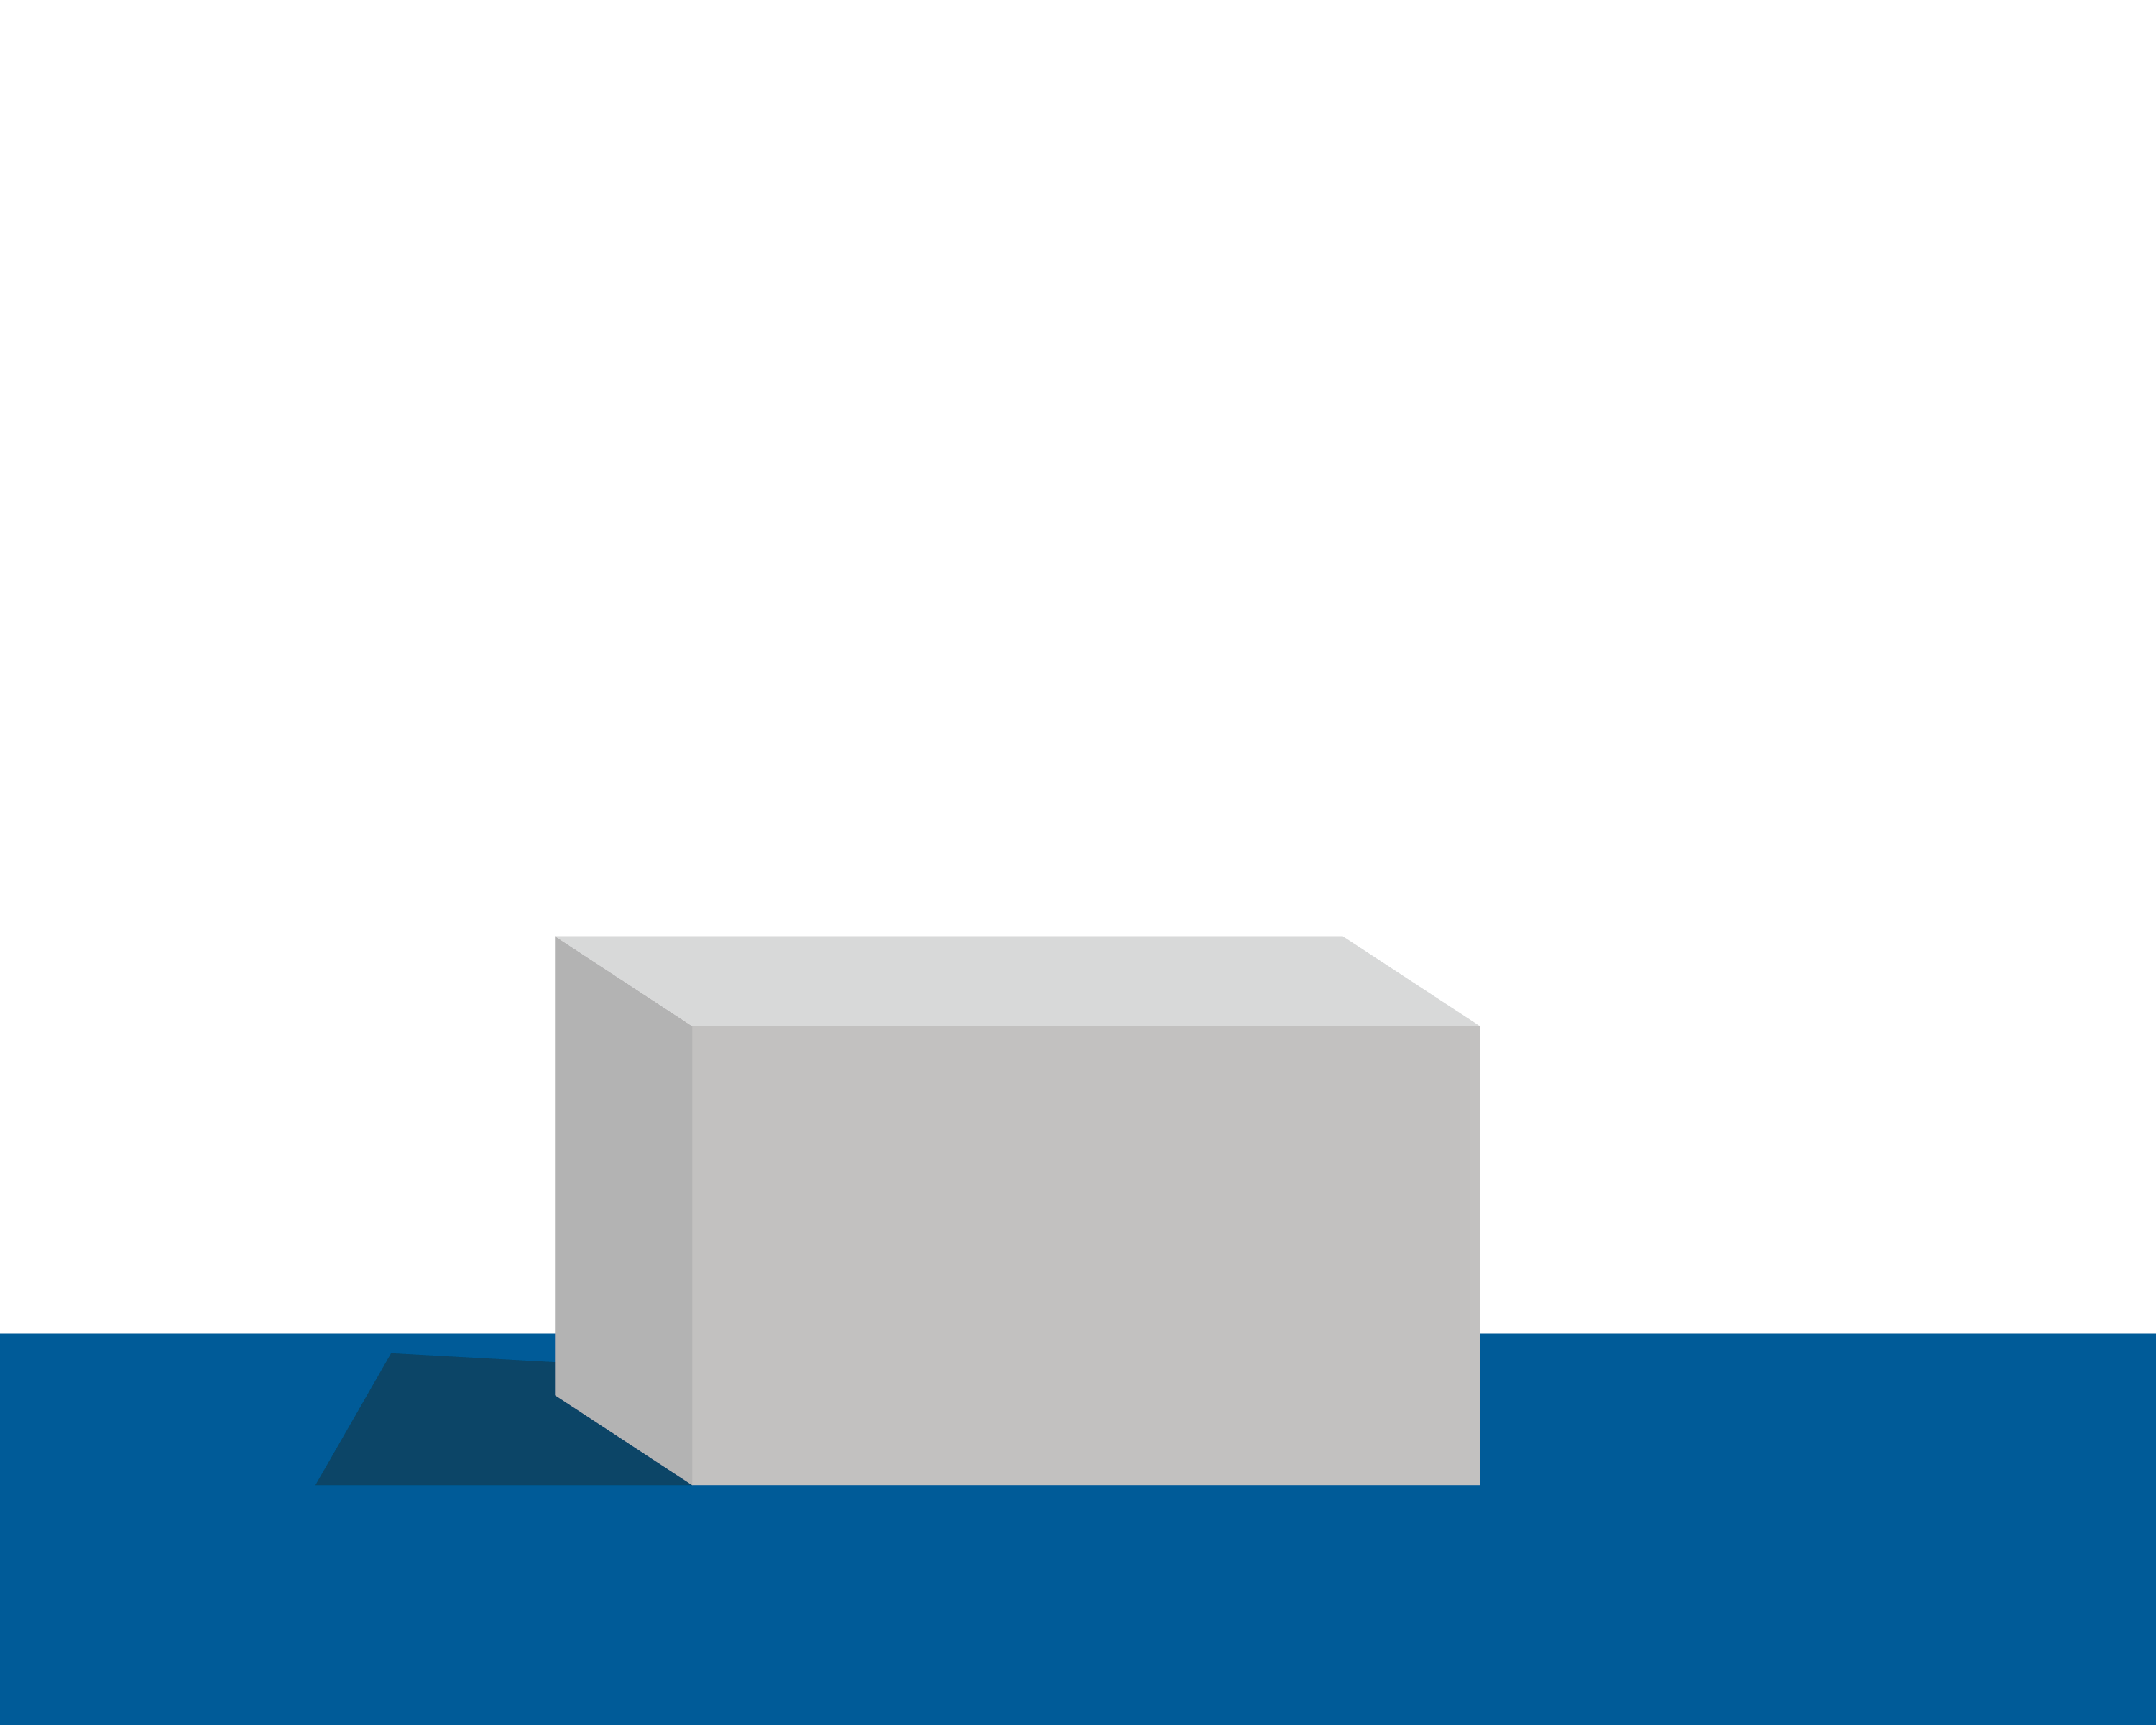
\includegraphics[width=0.75\textwidth]{friction-02.png}

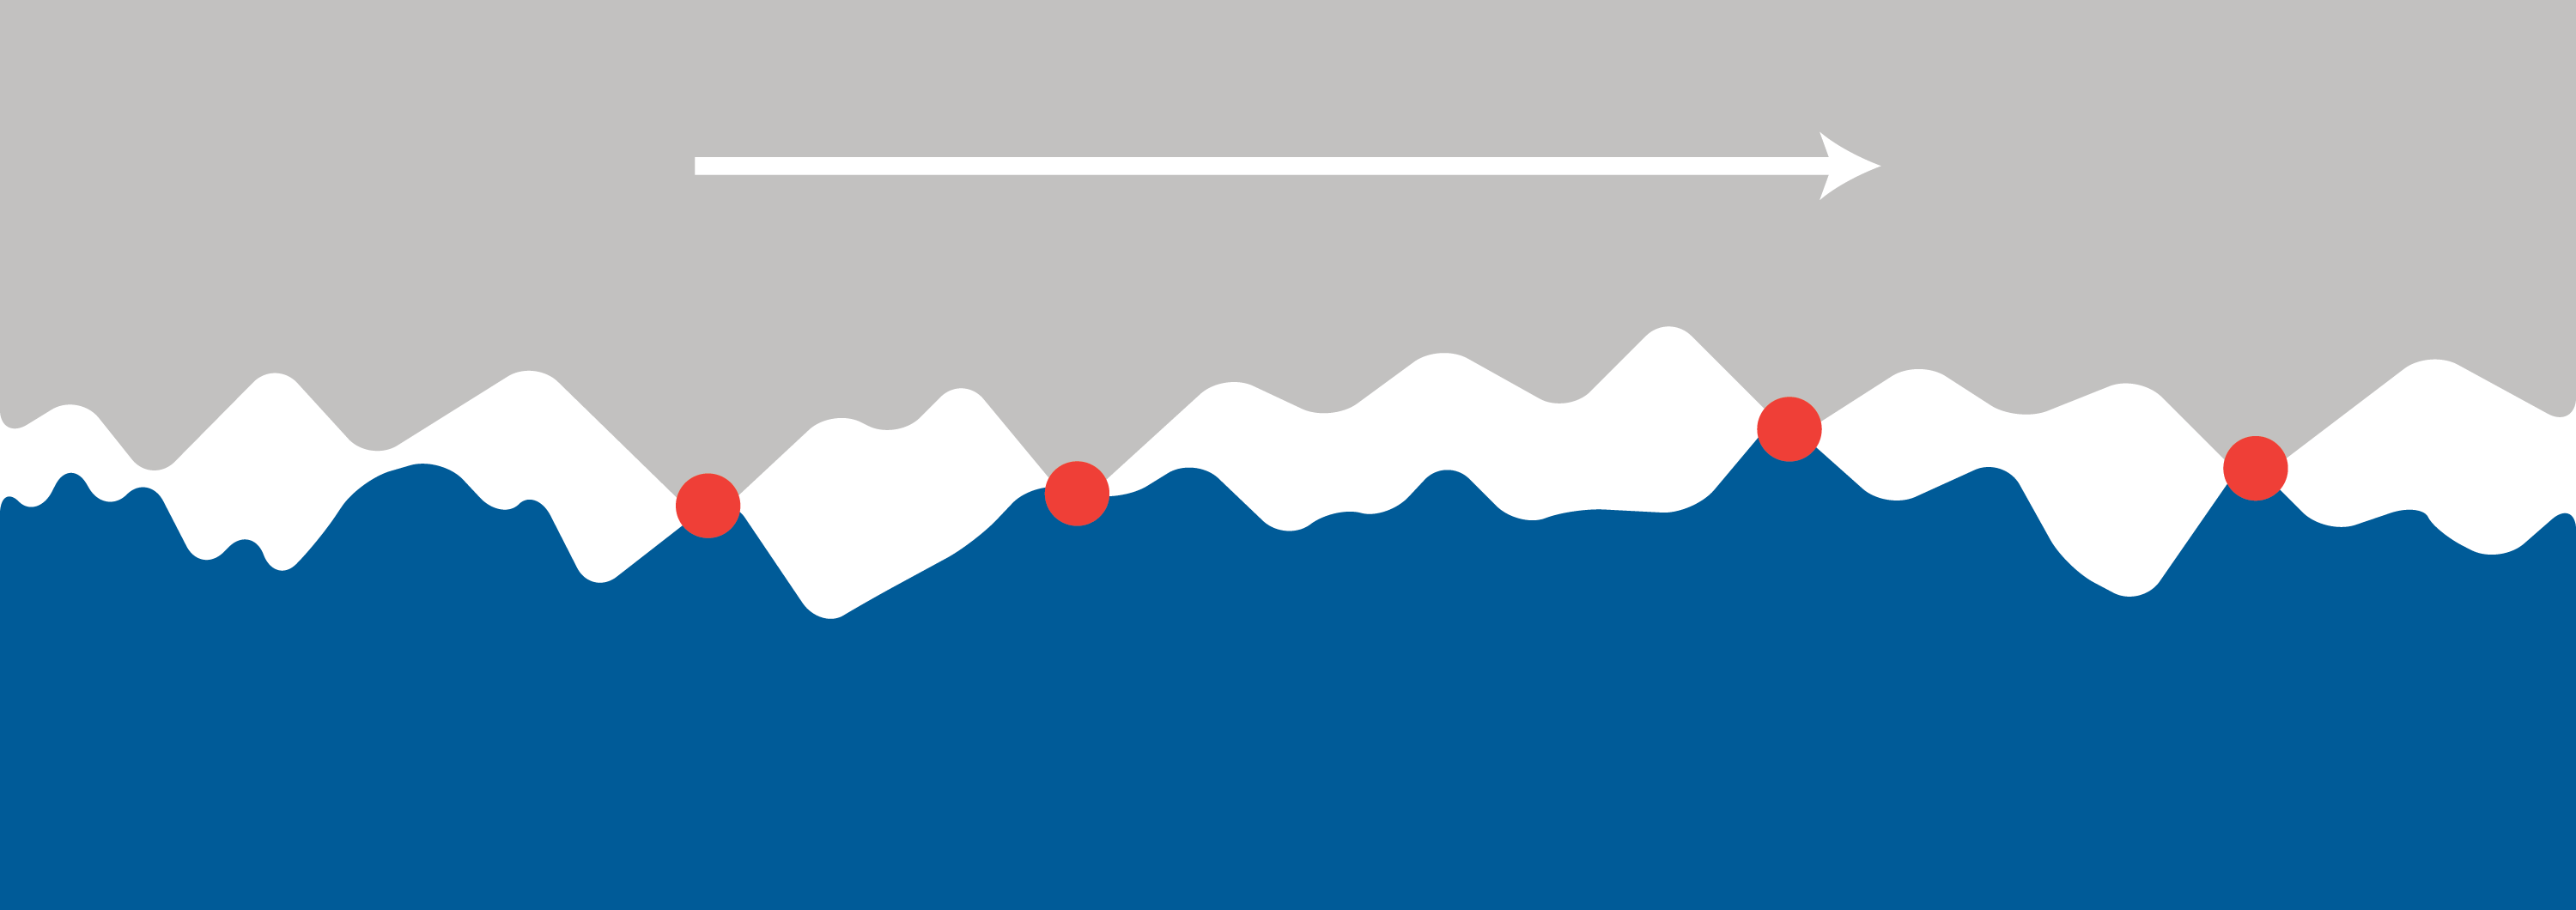
\includegraphics[width=0.75\textwidth]{friction-03.png}

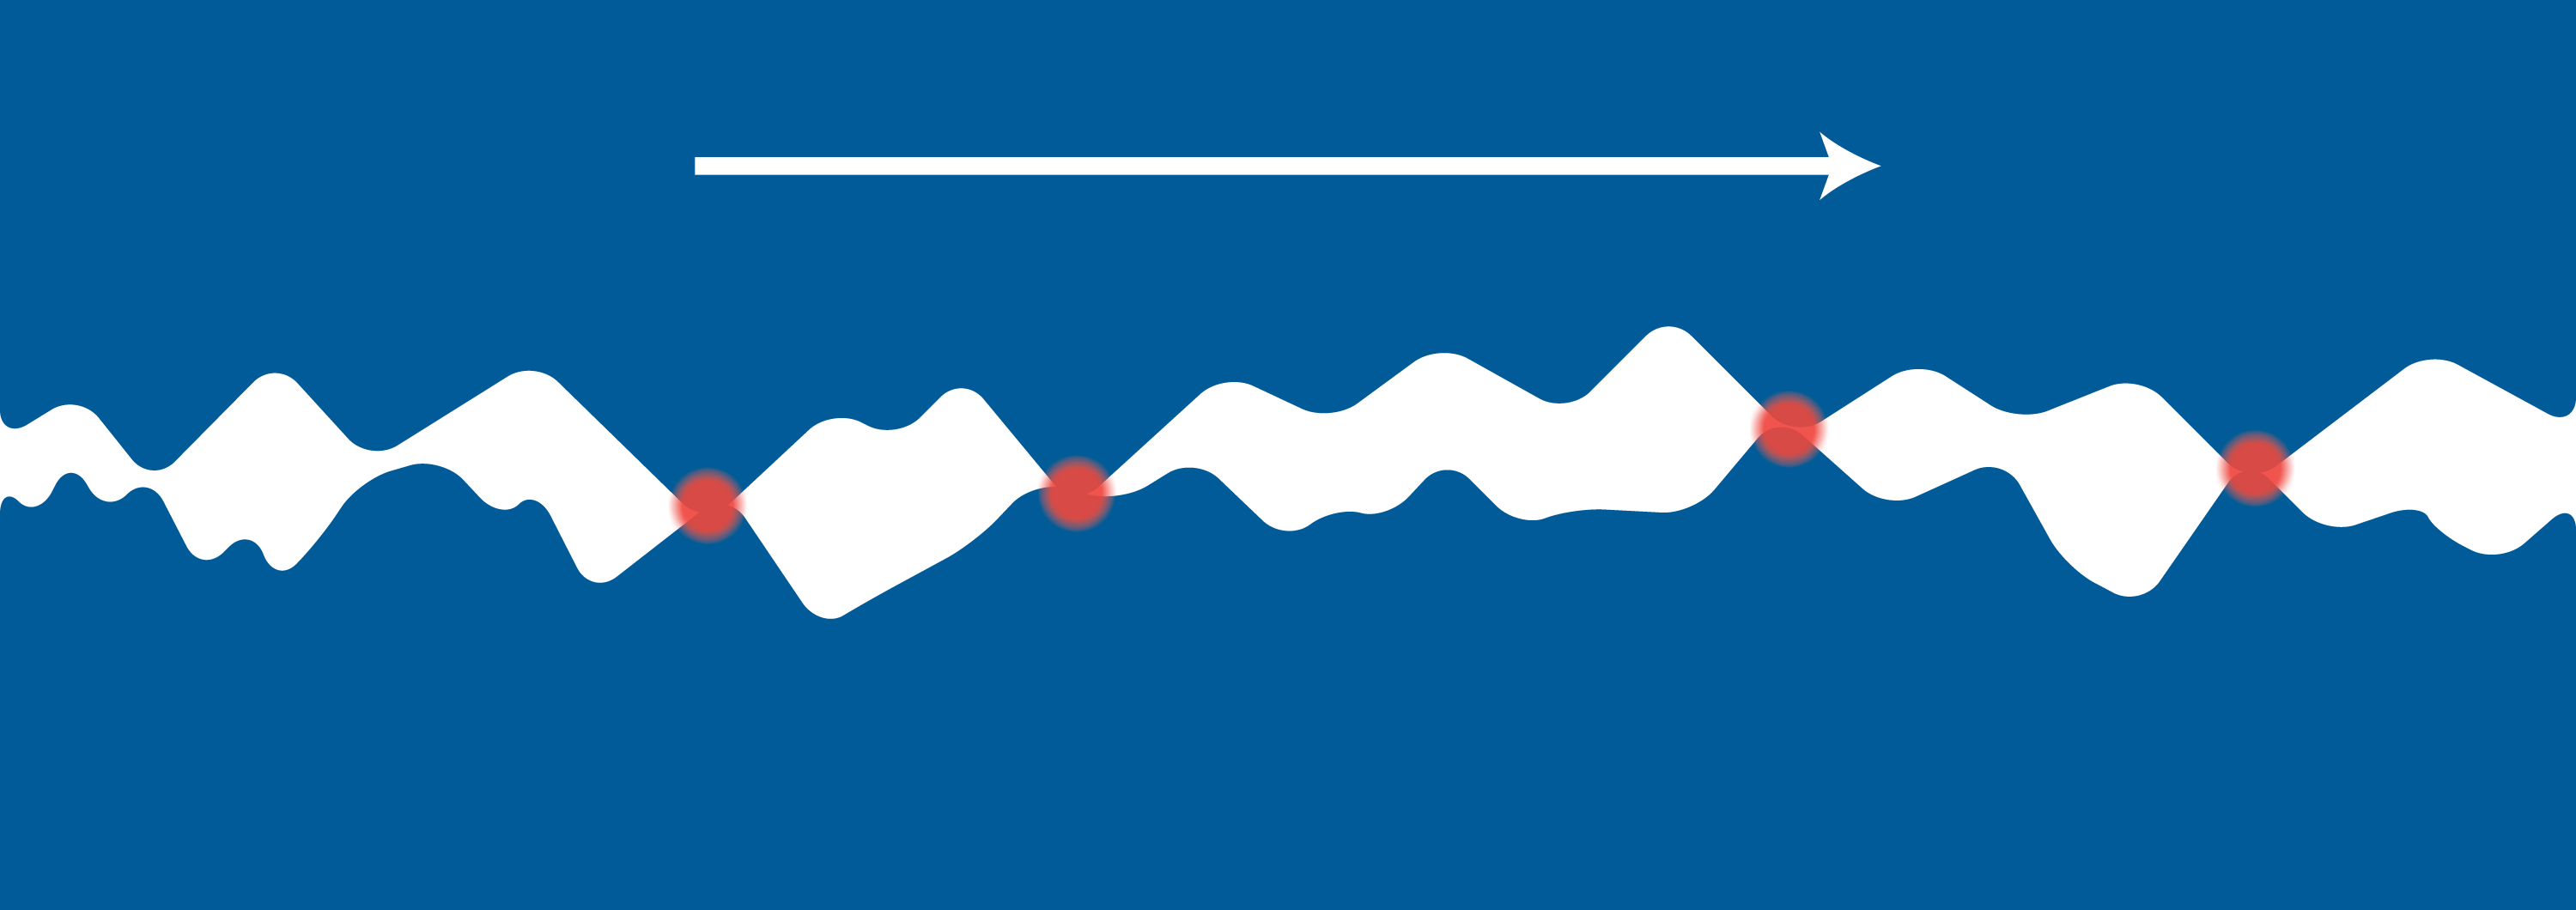
\includegraphics[width=0.75\textwidth]{friction-04.png}

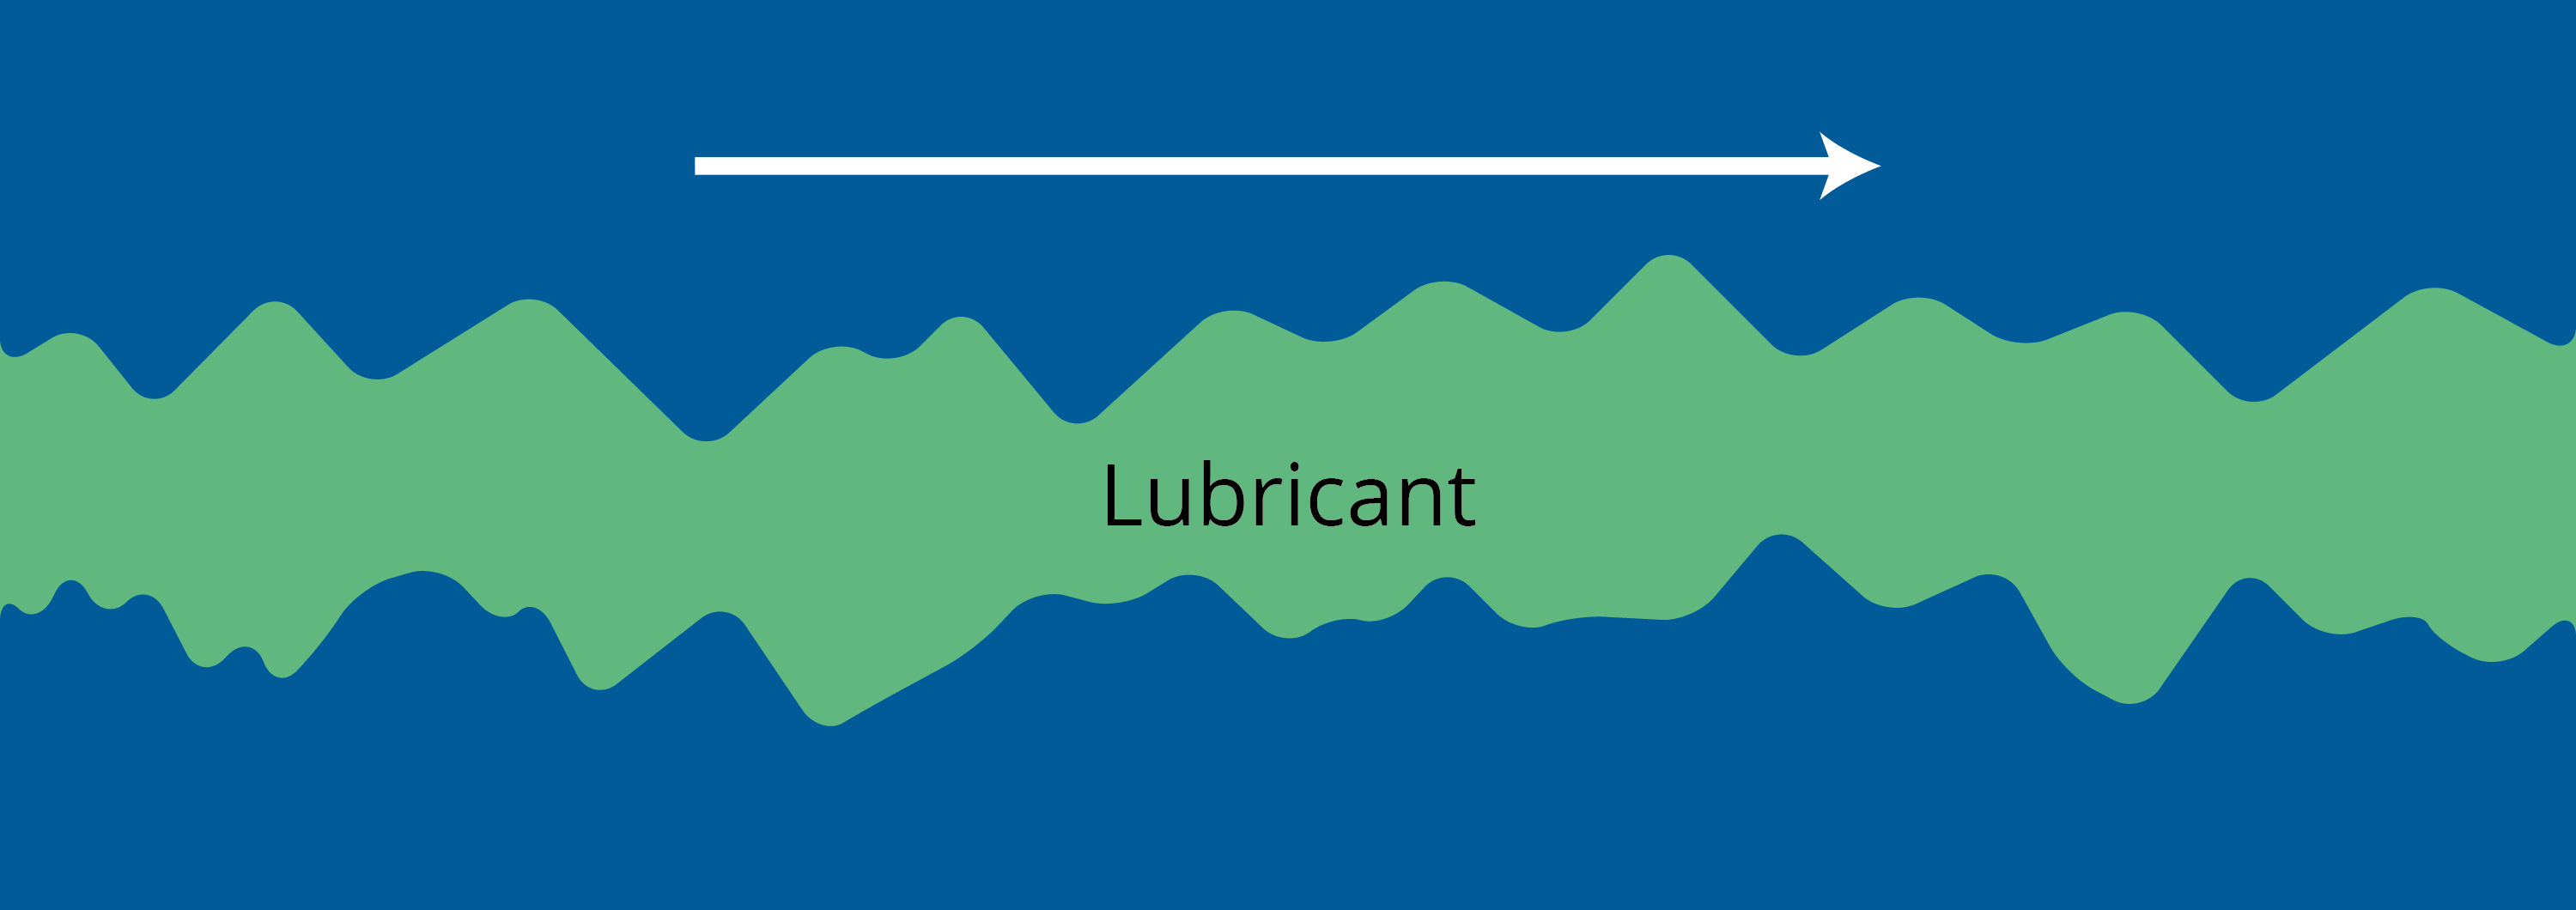
\includegraphics[width=0.75\textwidth]{friction-05.png}

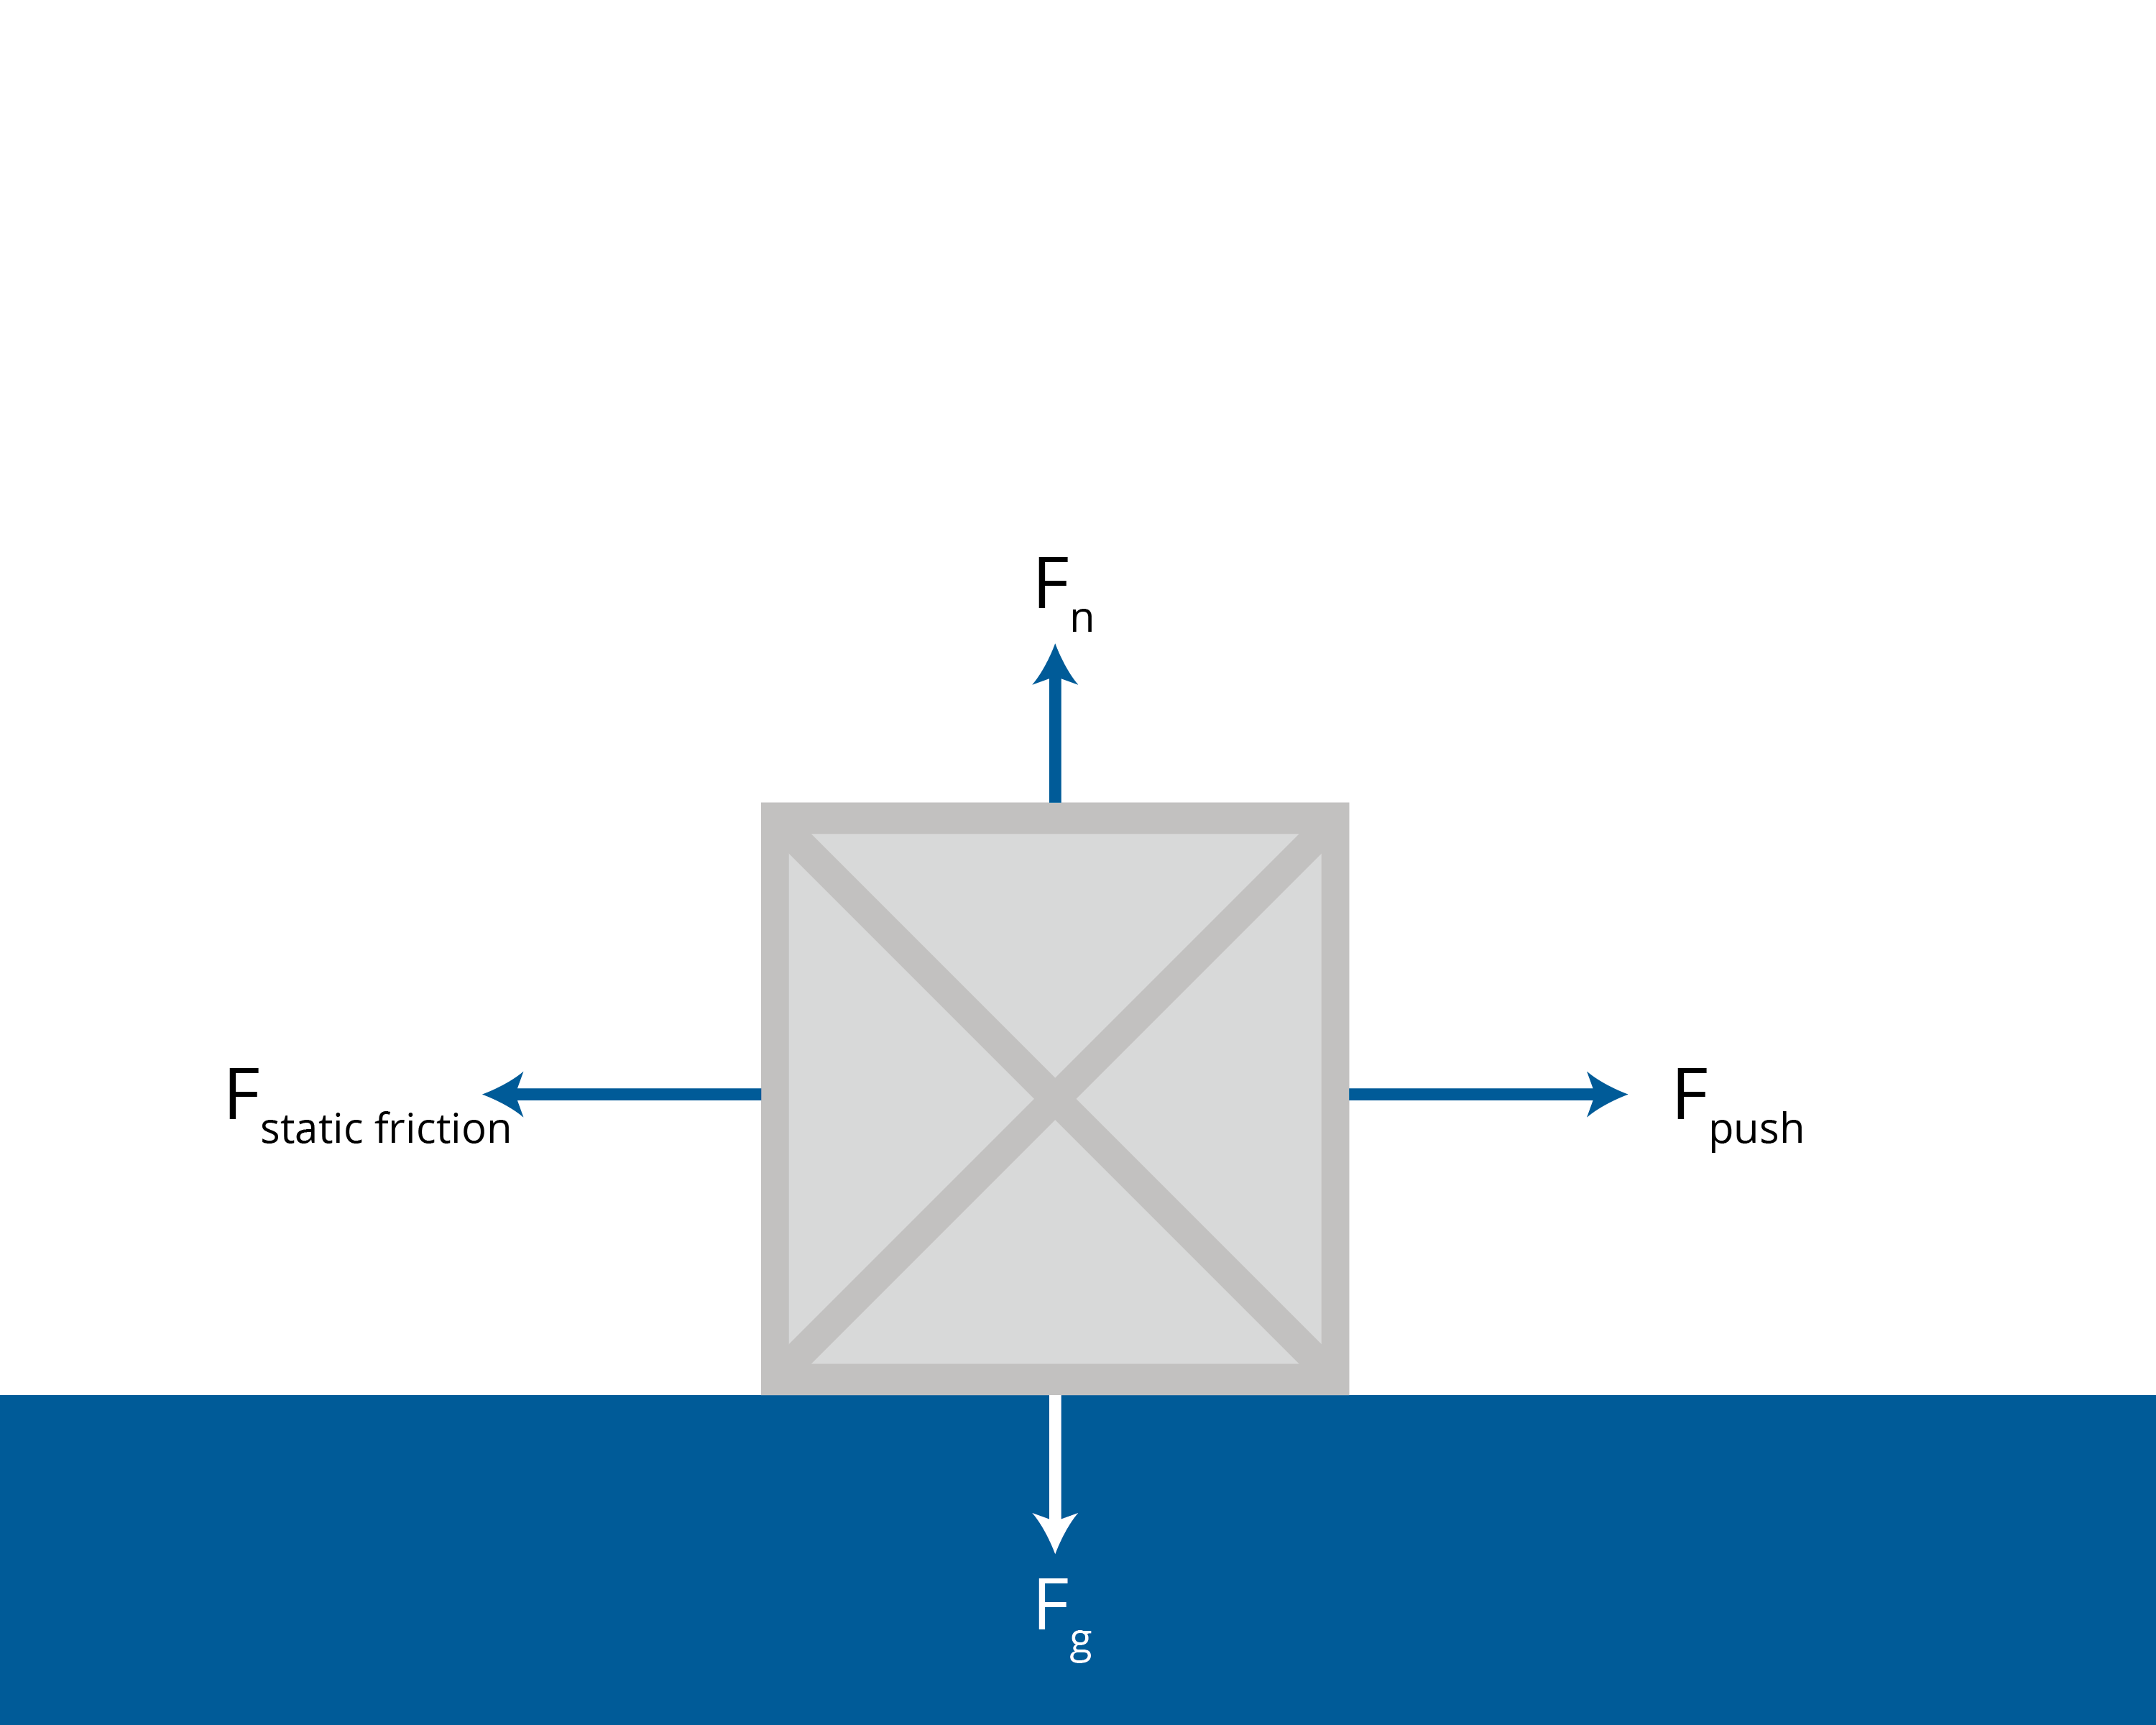
\includegraphics[width=0.75\textwidth]{friction-06.png}

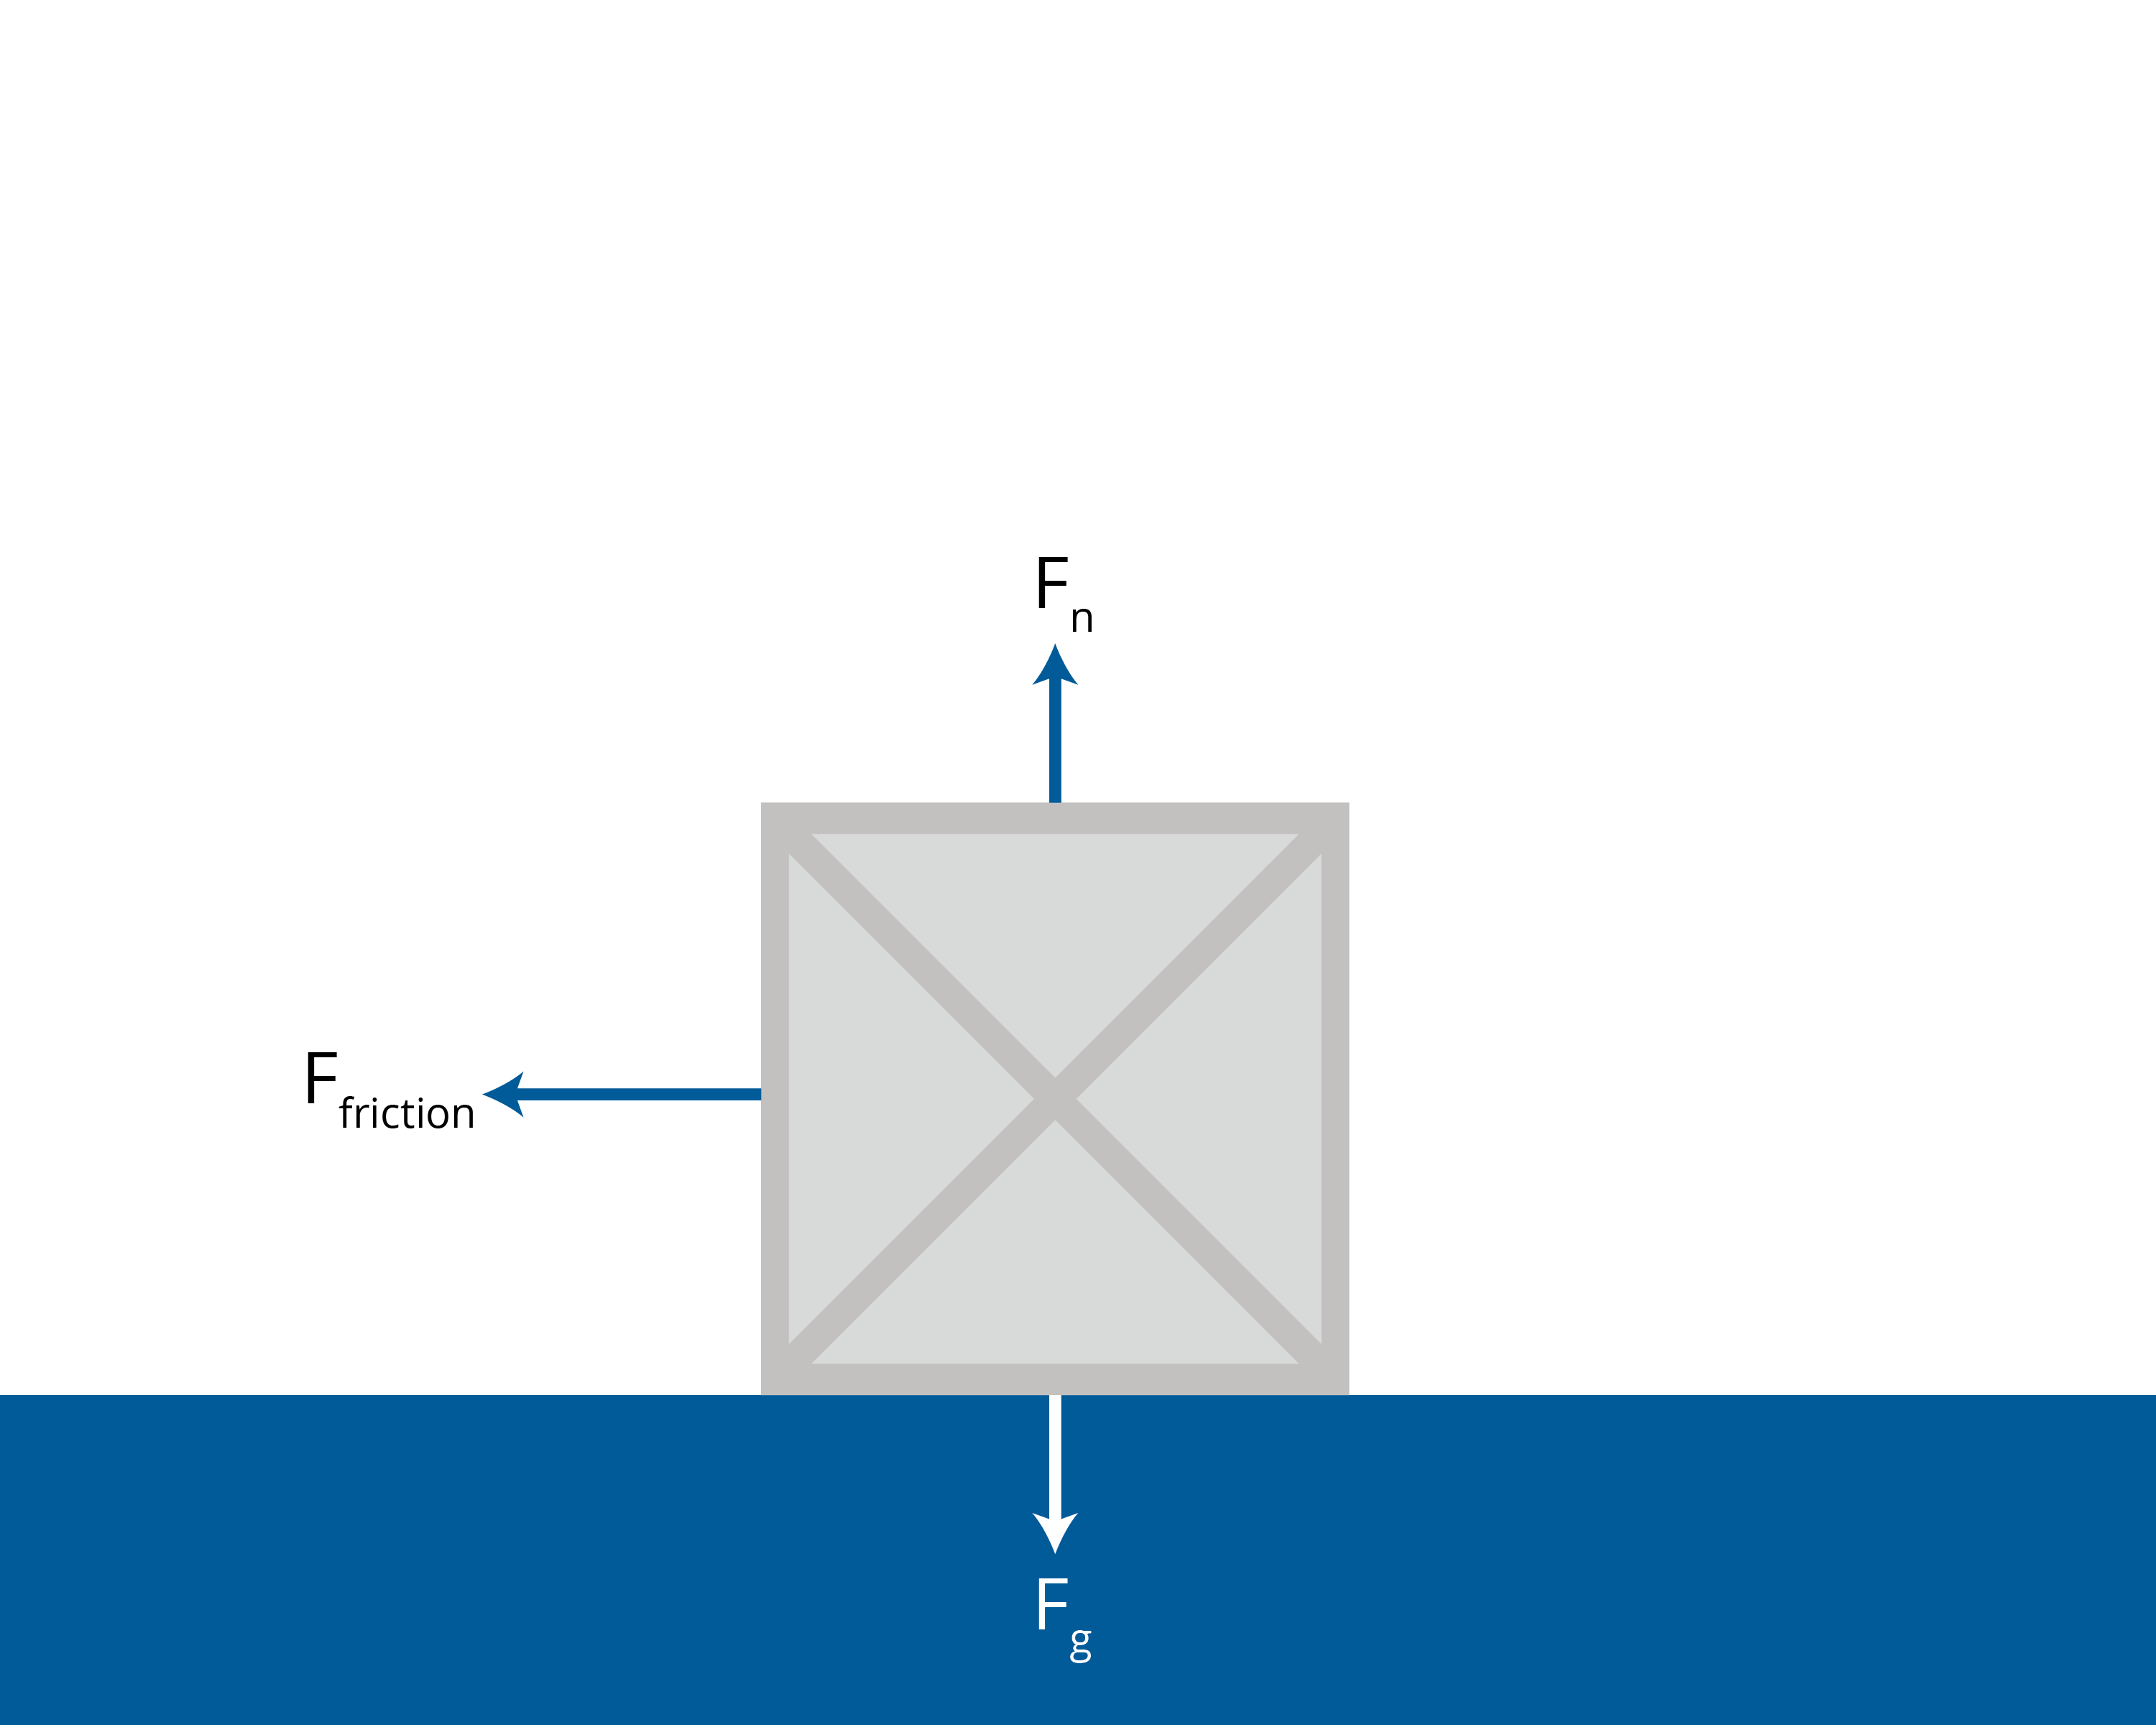
\includegraphics[width=0.75\textwidth]{friction-07.png}



% these graphics should be placed strategically in the text, not at the end








\graphicspath{{../../Chapters/greek/en_US}}
\chapter{The Greek Alphabet}

If you do anything involving math or physics, you will be encountering Greek letters on a regular basis. Here is a table for your reference:

\begin{tabular}{c c  l | c c l}
Capital & Lower & Pronounced & Capital & Lower & Pronounced\\
\hline
$A$ & $\alpha$ & Alpha & $N$ & $\nu$ & Nu\\
$B$ & $\beta$ & Beta & $\Xi$ & $\xi$ & Xi ("ku-ZY") \\
$\Gamma$ & $\gamma$ & Gamma & $O$ & $o$ & Omicron\\
$\Delta$ & $\delta$ & Delta & $\Pi$ & $\pi$ & Pi\\
$E$ & $\epsilon$ & Epsilon & $P$ & $\rho$ & Rho\\
$Z$ & $\zeta$ & Zeta & $\Sigma$ & $\sigma$ & Sigma\\
$H$ & $\eta$ & Eta & $T$ & $\tau$ & Tau\\
$\Theta$ & $\theta$ & Theta & $\Upsilon$ & $\upsilon$ & Upsilon\\
$I$ & $\iota$ & Iota & $\Phi$ & $\phi$ & Phi\\
$K$ & $\kappa$ & Kappa & $X$ & $\chi$ & Chi ("Kai")\\
$\Lambda$ & $\lambda$ & Lambda & $\Psi$ & $\psi$ & Psi ("Sigh")\\
$M$ & $\mu$ & Mu & $\Omega$ & $\omega$ & Omega
\end{tabular}
% maybe move this to the first book. probably most important
\graphicspath{{../../Chapters/basic_statistics/en_US}}
\chapter{Basic Statistics}

You live near a freeway, and someone asks you, ``How fast do cars on that freeway drive?''

You say, ``Pretty fast.''

They reply, ``Can you be more specific?''

So, you pull out your radar gun you happen to always keep on you, and tell them, ``That one is going 32.131 meters per second.''

To which they say, ``I don't want to know about that specific car. I want to know about all the cars.''

So, you spend the day beside the freeway measuring the speed of every
car that goes by. And you get a list of a thousand numbers, including:

\begin{tabular}{c | c | c}
30.462 m/s  & 29.550 m/s & 29.227 m/s \\
37.661 m/s  & 27.899 m/s & 28.113 m/s \\
24.382 m/s & 35.668 m/s & 43.797 m/s \\
31.312 m/s & 37.637 m/s & 30.891 m/s
\end {tabular}

There are 12 numbers here. We say that there are 12 \textit{samples}.\index{samples}

\section{Mean}

We often talk about the \textit{average} of a set of samples, which is the 
same as the \textit{mean}. To get the mean, sum up the
samples and divide that number by the number of samples.\index{mean}

The numbers in that table sum to $388.599$.  If you divide that by 12,
you find that the mean of those samples is 32.217 m/s.

We typically use the greek letter $\mu$ (``mu'') to represent the mean.

\begin{mdframed}[style=important, frametitle={Definition of Mean}]
  
If you have a set of samples $x_1, x_2, \ldots, x_n$, the mean is:

$$ \mu = \frac{1}{n} \sum_{i=1}^n x_i$$

\end{mdframed}

This may be the first time you are seeing a summation ($\sum$). The equation above is equivalent to:\index{summation symbol}

$$ \mu = \frac{1}{n} \left(x_1 + x_2 + \ldots + x_n\right)$$

\begin{Exercise}[title={Mean Grade}, label=grades_mean]

  Teachers often use the mean for grading. For example, if you took
  six quizzes in a class, your final grade might be the mean of the six
  scores. Find the mean of these six grades: 87, 91, 98, 65, 87, 100.

\end{Exercise}
\begin{Answer}[ref=grades_mean]

  $$\mu =\frac{1}{6} \left(87 + 91 + 98 + 65 + 87 + 100 \right) = 88$$

\end{Answer}

If you tell your friend, ``I measured the speed of 1000 cars, and the
mean is 31.71 m/s'', your friend will wonder, ``Are most of the speeds
clustered around 31.71? Or are they all over the place and just happen
to have a mean of 31.71?'' To answer this question, we use variance.

\section{Variance}

\begin{mdframed}[style=important, frametitle={Definition of Variance}]

If you have $n$ samples $x_1, x_2, \ldots, x_n$ that have a mean of $\mu$, the \textit{variance} is defined to be:\index{variance}

$$v = \frac{1}{n}\sum_{i = 1}^{n} \left(x_i - \mu\right)^2$$
% ADD: Maybe connect to Chi-squared test
\end{mdframed}

That is, you figure out how far each sample is from the median, you
square that, and then you take the mean of all those squared
distances.

\begin{tabular} {c | c | c}

  $x$ & $x - \mu$ & $(x - \mu)^2$\\
  \hline
30.462 & -1.755 & 3.079 \\
29.550 & -2.667 & 7.111\\
29.227 & -2.990 & 8.938\\
37.661 & 5.444 & 29.642\\
27.899 & -4.318 & 18.642\\
28.113 & -4.104 & 16.839 \\
24.382 & -7.835 & 61.381 \\
35.668 & 3.451 & 11.912 \\
43.797 & 11.580 & 134.106\\
31.312 & -0.905 & 0.818\\
37.637 & 5.420 & 29.381\\
30.891 & -1.326 & 1.757\\
\hline
$\sum x = 386.599$ & & $\sum (x - \mu)^2 = 323.605$\\
mean = 32.217 & & variance = 26.967
\end{tabular}

Thus, the variance of the 12 samples is 26.967. The bigger the variances, 
the farther the samples are spread apart; the smaller the variances, the closer
samples are clustered around the mean.

Notice that most of the data points deviate from the mu by 1 to 5
m/s. Isn't it odd that the variance is a big number like 26.967?
Remember that it represents the average of the squares. Sometimes, to
get a better feel for how far the samples are from the mean, we use
the square root of the variance, which is called \textit{the standard
  deviation}.

The standard deviation of your 12 samples would be $\sqrt{26.9677} =
  5.193$ m/s.
% ADD: Bell curve, KA: https://www.khanacademy.org/computer-programming/spin-off-of-galton-board-exploration/1930953307/embedded?embed=yes&article=yes&editor=no&buttons=no&author=no&width=400&height=400

The standard deviation is used to figure out a data point is an
outlier. For example, if you are asked, ``That car that just sped
past. Was it going freakishly fast?'' You might respond, ``No, it was
within a standard deviation of the mean.'' or ``Yes, its speed was 2
standard deviations more than the mean. They will probably get a ticket.''
% ADD: Box and whiskers plot?

A singular $\mu$ usually represents the mean. $\sigma$ usually represents
the standard deviation. So $\sigma^2$ represents the variance.

\begin{Exercise}[title={Variance of Grades}, label=grades_variance]

  Now, find the variance for your six grades. As a reminder, they were: 87, 91, 98, 65, 87, 100.

  What is your standard deviation?

\end{Exercise}
\begin{Answer}[ref=grades_variance]

  The mean of your grades is $88$.

  The variance, then, is

  $$\sigma^2 = \frac{1}{6} \left((87 - 88)^2 + (91 - 88)^2 + (98 - 88)^2 + (61 - 88)^2 + (87 - 88)^2 + (100 - 88)^2 \right) = \frac{784}{6} = 65 \frac{1}{3}$$

  The standard deviation is the square root of that: $\sigma = 8.083$ points.
  
\end{Answer}


\section{Median}

Sometimes you want to know where the middle is. For example, you want
to know the speed at which half the cars are going faster and half are
going slower. To get the median, you sort your samples from smallest
to largest. If you have an odd number of samples, the one in the
middle is the median. If you have an even number of samples, we take
the mean of the two numbers in the middle.\index{median}
% KA: https://www.khanacademy.org/math/cc-sixth-grade-math/cc-6th-data-statistics/mean-and-median/v/statistics-intro-mean-median-and-mode

In our example, you would sort your numbers and find the two in the middle:

\begin{tabular}{c}
24.382\\
27.899\\
28.113\\
29.227\\
29.550\\
\hline
\textbf{30.462}\\
\textbf{30.891}\\
\hline 
31.312\\
35.668\\
37.637\\
37.661\\
43.797\\
\end{tabular}

You take the mean of the two middle numbers: $(30.462 + 30.891)/2 =
30.692$. The median speed would be 30.692 m/s.

Medians are often used when a small number of outliers majorly skew the
mean. For example, income statistics usually use the median income
because a few hundred billionares raise the mean a great deal.

\begin{Exercise}[title={Median Grade}, label=grades_median]

  Find the median of your six grades: 87, 91, 98, 65, 87, 100.

\end{Exercise}
\begin{Answer}[ref=grades_median]

  In order the grades are 65, 87, 87, 91, 98, 100.  The middle two are 87
  and 91. The mean of those is 89. (Speed trick: The mean of two numbers is the
  number that is halfway between.)
  
 \end{Answer}


\section{Histograms}

A histogram is a bar chart that shows how many samples are in each
group. In our example, we group cars by speed. Maybe we count the
number of cars going between 30 and 32 m/s. Next, we count the
cars going between 32 and 34 m/2. Finally, we make a bar chart from
that data.\index{histograms}
% ADD: Have not explained histograms yet

Your 1000 cars would break up into these groups:

\begin{tabular}{ c | c }
0 - 2 m/s & 0 cars \\
2 - 4 m/s & 0 cars \\
4 - 6 m/s & 0 cars \\
\ldots & \ldots \\
20 - 22 m/s & 0 cars \\
22 - 24 m/s & 0 cars \\
24 - 26 m/s & 65 cars \\
26 - 28 m/s & 160 cars \\
28 - 30 m/s & 175 cars \\
30 - 32 m/s & 168 cars \\
32 - 34 m/s & 150 cars \\
34 - 36 m/s & 114 cars \\
36 - 38 m/s & 79 cars \\
38 - 40 m/s & 52 cars \\
40 - 42 m/s & 20 cars \\
42 - 44 m/s & 12 cars \\
44 - 46 m/s & 4 cars \\
46 - 48 m/s & 1 cars \\
48 - 50 m/s & 0 cars \\
\end{tabular}

Next, we make a bar chart from that:

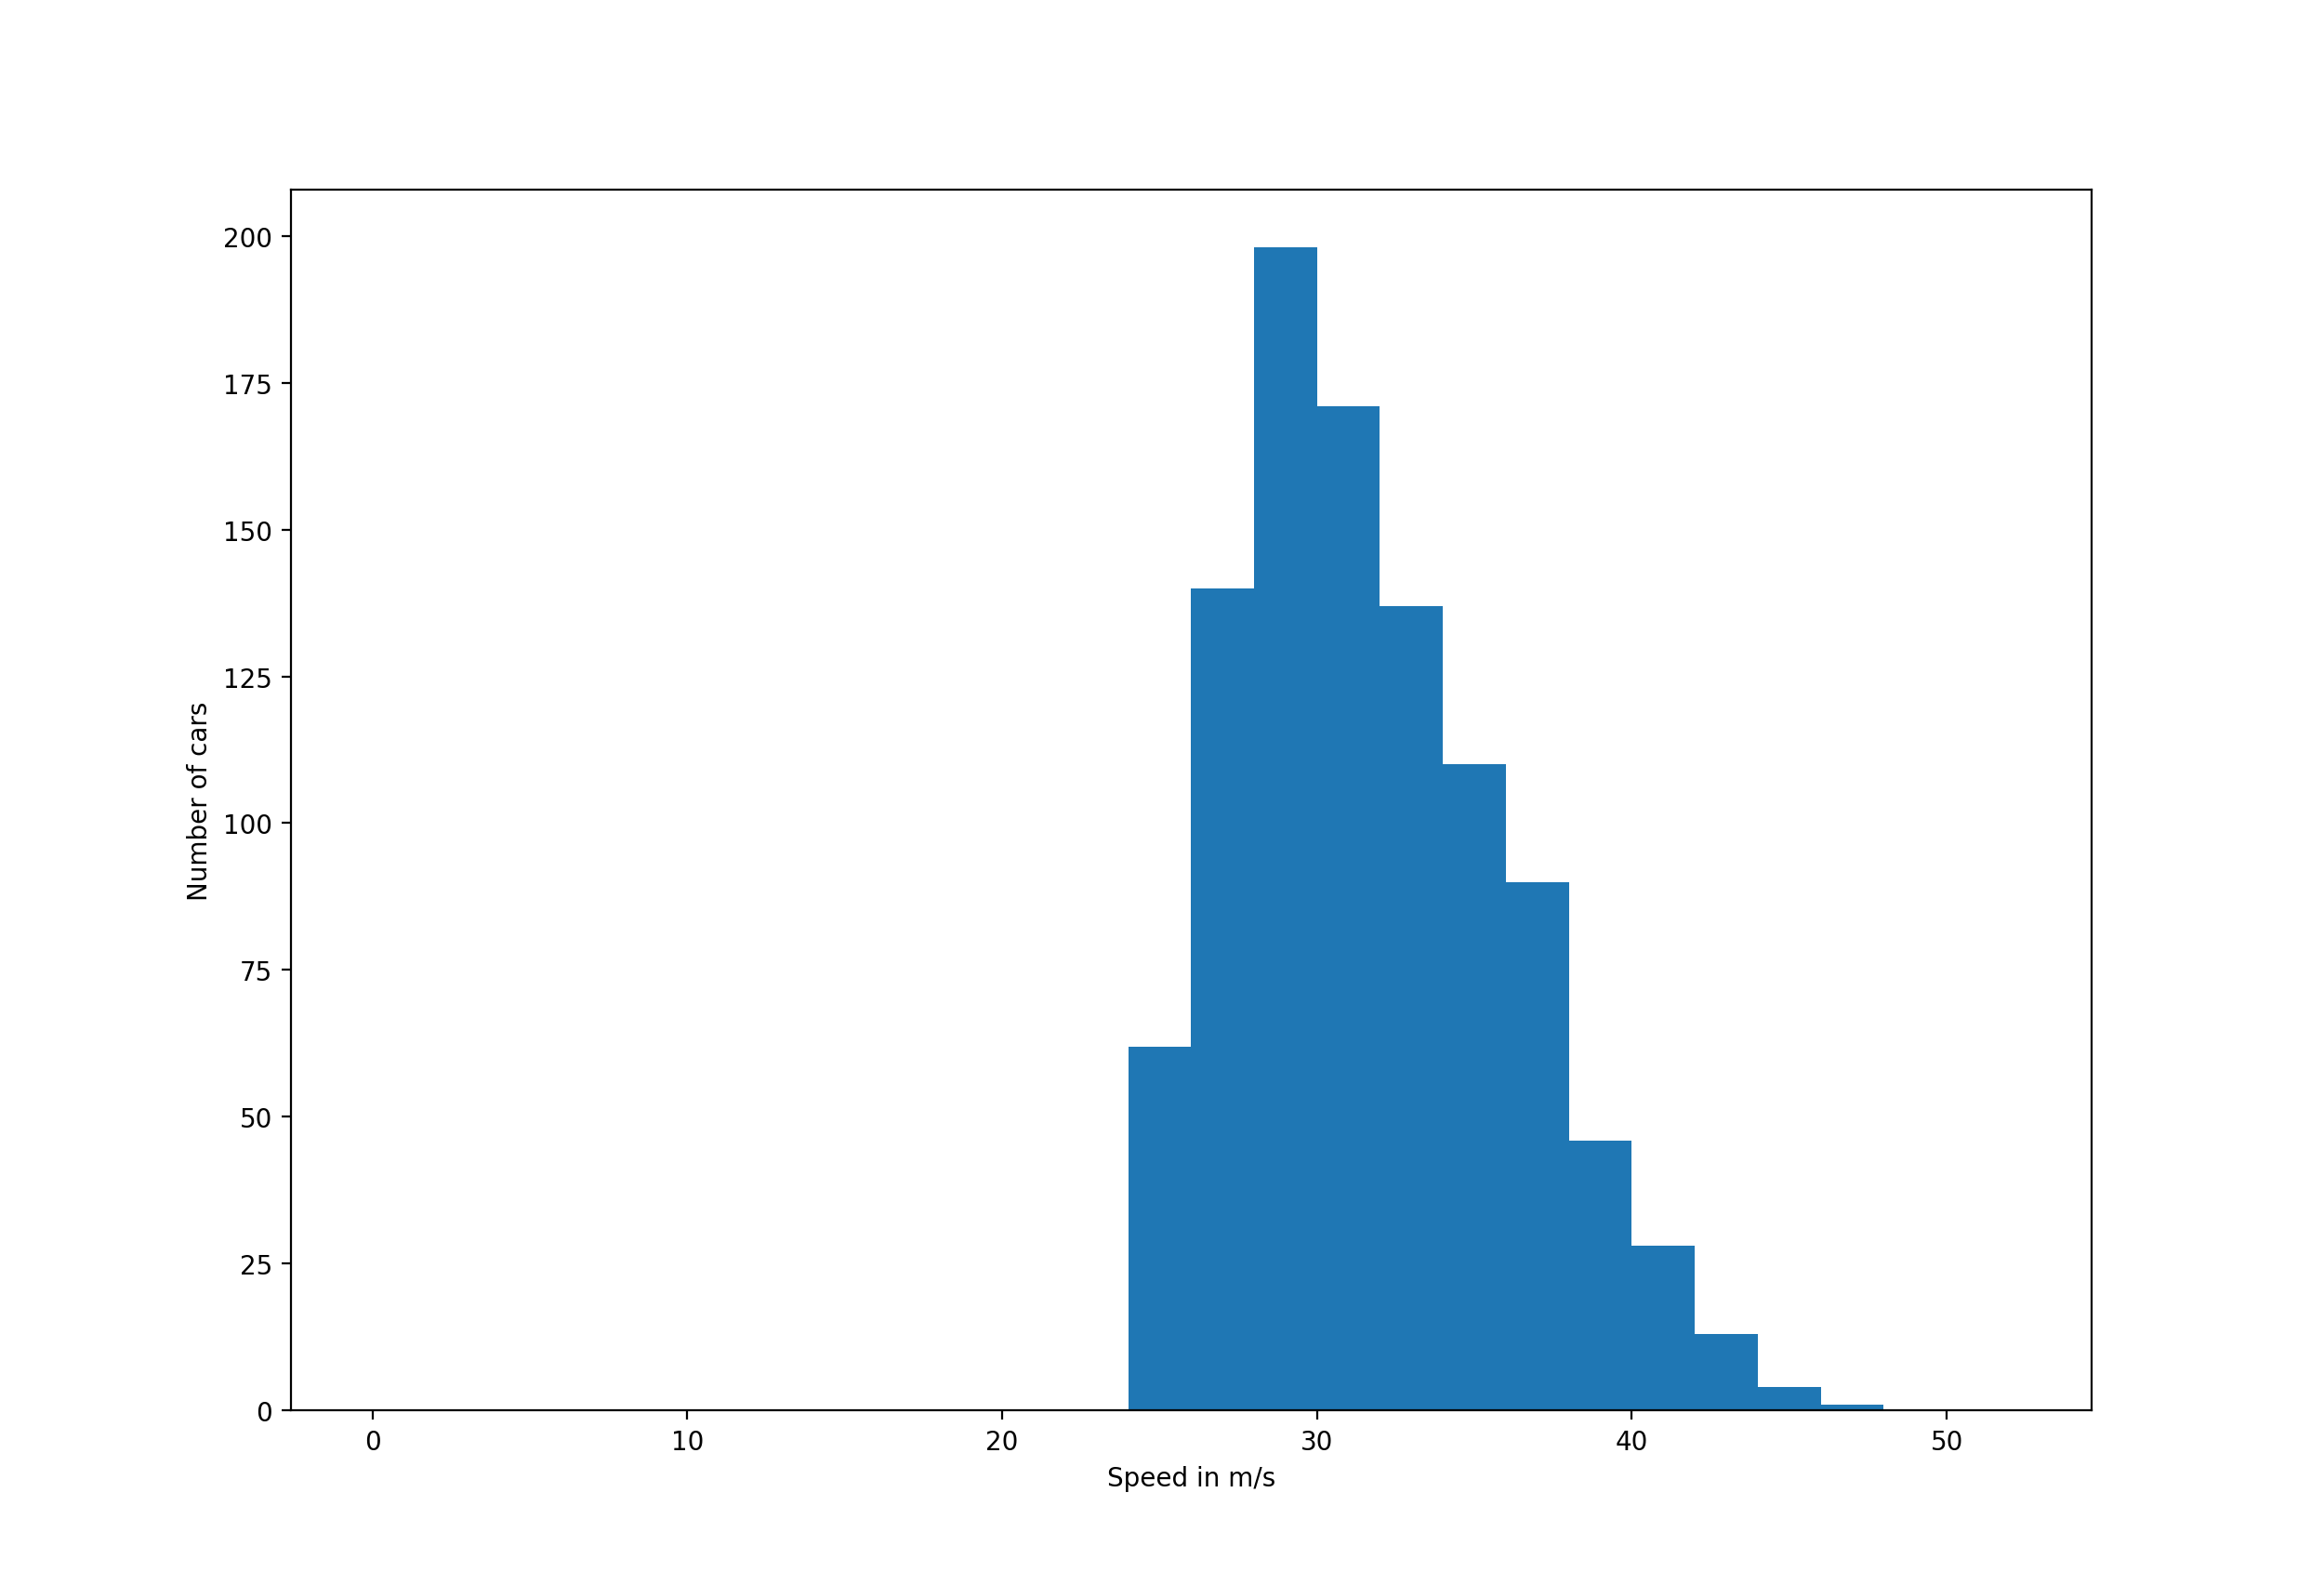
\includegraphics[width=\textwidth] {speed_histo.png}

Often, a histogram will tell the story of the data. Here, you can see
that no one is going less than 24 m/s, but a lot of people travel at
30 m/s. There are a few people who travel over 40 m/s, but there are also a
couple of people who drive much faster than anyone else.

\section{Root-Mean-Squared}

Scientists have a mean-like statistic that they love. It is named
quadratic mean, but most just calls it Root-Mean-Squared, or
RMS.

\begin{mdframed}[style=important, frametitle={Definition of RMS}]

If you have a list of numbers $x_1, x_2, \ldots, x_n$, their RMS
is \index{quadratic mean} \index{root-mean-squared} \index{RMS}

$$\sqrt{\frac{1}{n}\left( x_1^2 + x_2^2 + \ldots + x_n^2 \right)}$$

\end{mdframed}

You are taking the square root of the mean of squares of the samples,
thus the name Root-Mean-Squared.

Using your 12 samples:

\begin{tabular}{c |  c}
  $x$ & $x^2$ \\
  \hline
30.462 & 927.933 \\
29.550 & 873.203\\
29.227 & 854.218\\
37.661 & 1418.351\\
27.899 & 778.354\\
28.113 & 790.341\\
24.382 & 594.482\\
35.668 & 1272.206\\
43.797 & 1918.177\\
31.312 & 980.441\\
37.637 & 1416.544\\
30.891 & 954.254\\
\hline
\multicolumn{1}{r}{Mean of $x^2$} & {1064.875}\\
\multicolumn{1}{r}{RMS} & {32.632}
  \end{tabular}

Why is RMS useful? Let's say that all cars had the same mass $m$, and
you need to know what the average kinetic energy per car is. If you
know the RMS of the speeds of the cars is $v_{rms}$, the average kinetic energy for
each car is

$$k = \frac{1}{2}m v_{rms}^2$$

(You don't believe me? Let's prove it. Substitute in the RMS:

$$k = \frac{1}{2}m \sqrt{\frac{1}{n}\left( x_1^2 + x_2^2 + \ldots + x_n^2 \right)}^2$$

The square root and the square cancel each other out:

$$k = \frac{1}{2}m \frac{1}{n}\left( x_1^2 + x_2^2 + \ldots + x_n^2 \right)$$

Use the distributive property:

$$k = \frac{1}{n} \left( \frac{1}{2} m x_1^2 + \frac{1}{2}m x_2^2 + \ldots + \frac{1}{2}m x_n^2 \right)$$


That is all the kinetic energy divided by the number of cars, which is
the mean kinetic enegy per car. Quod erat demonstrandum! (That is a
Latin phrase that means ``which is what I was trying to
demonstrate''. You will sometimes see ``QED'' at the end of a long
mathematic proof.)

Now you are ready for the punchline: Kinetic energy and heat are the
same thing. Instead of cars, heat is the kinetic energy of molecules
moving around. More on this soon.

Video: Mean, Median, Mode: https://www.youtube.com/watch?v=5C9LBF3b65s



\graphicspath{{../../Chapters/stat_spreadsheets/en_US}}
\chapter{Basic Statistics in Spreadsheets}

When you completed the problems in the last section, you probably noticed
how long it took to compute statistics like the mean, the median,
and variance by hand. Luckily, computers were designed to free us from these
sorts of tedious tasks. The most basic tool for automating
calculations is the spreadsheet program.\index{spreadsheet}

There are lots of spreadsheet programs including Microsoft's Excel and
Apple's Numbers. Any spreadsheet program will work; they are all very
similar. The instructions and screenshots here will be from Google
Sheets -- a free spreadsheet program you use through your web browser.

\section{Your First Spreadsheet}

In whatever spreadsheet program you are using, create a new spreadsheet document.

A spreadsheet is essentially a grid of cells. In each cell you can put data (like numbers or text) and formulas.

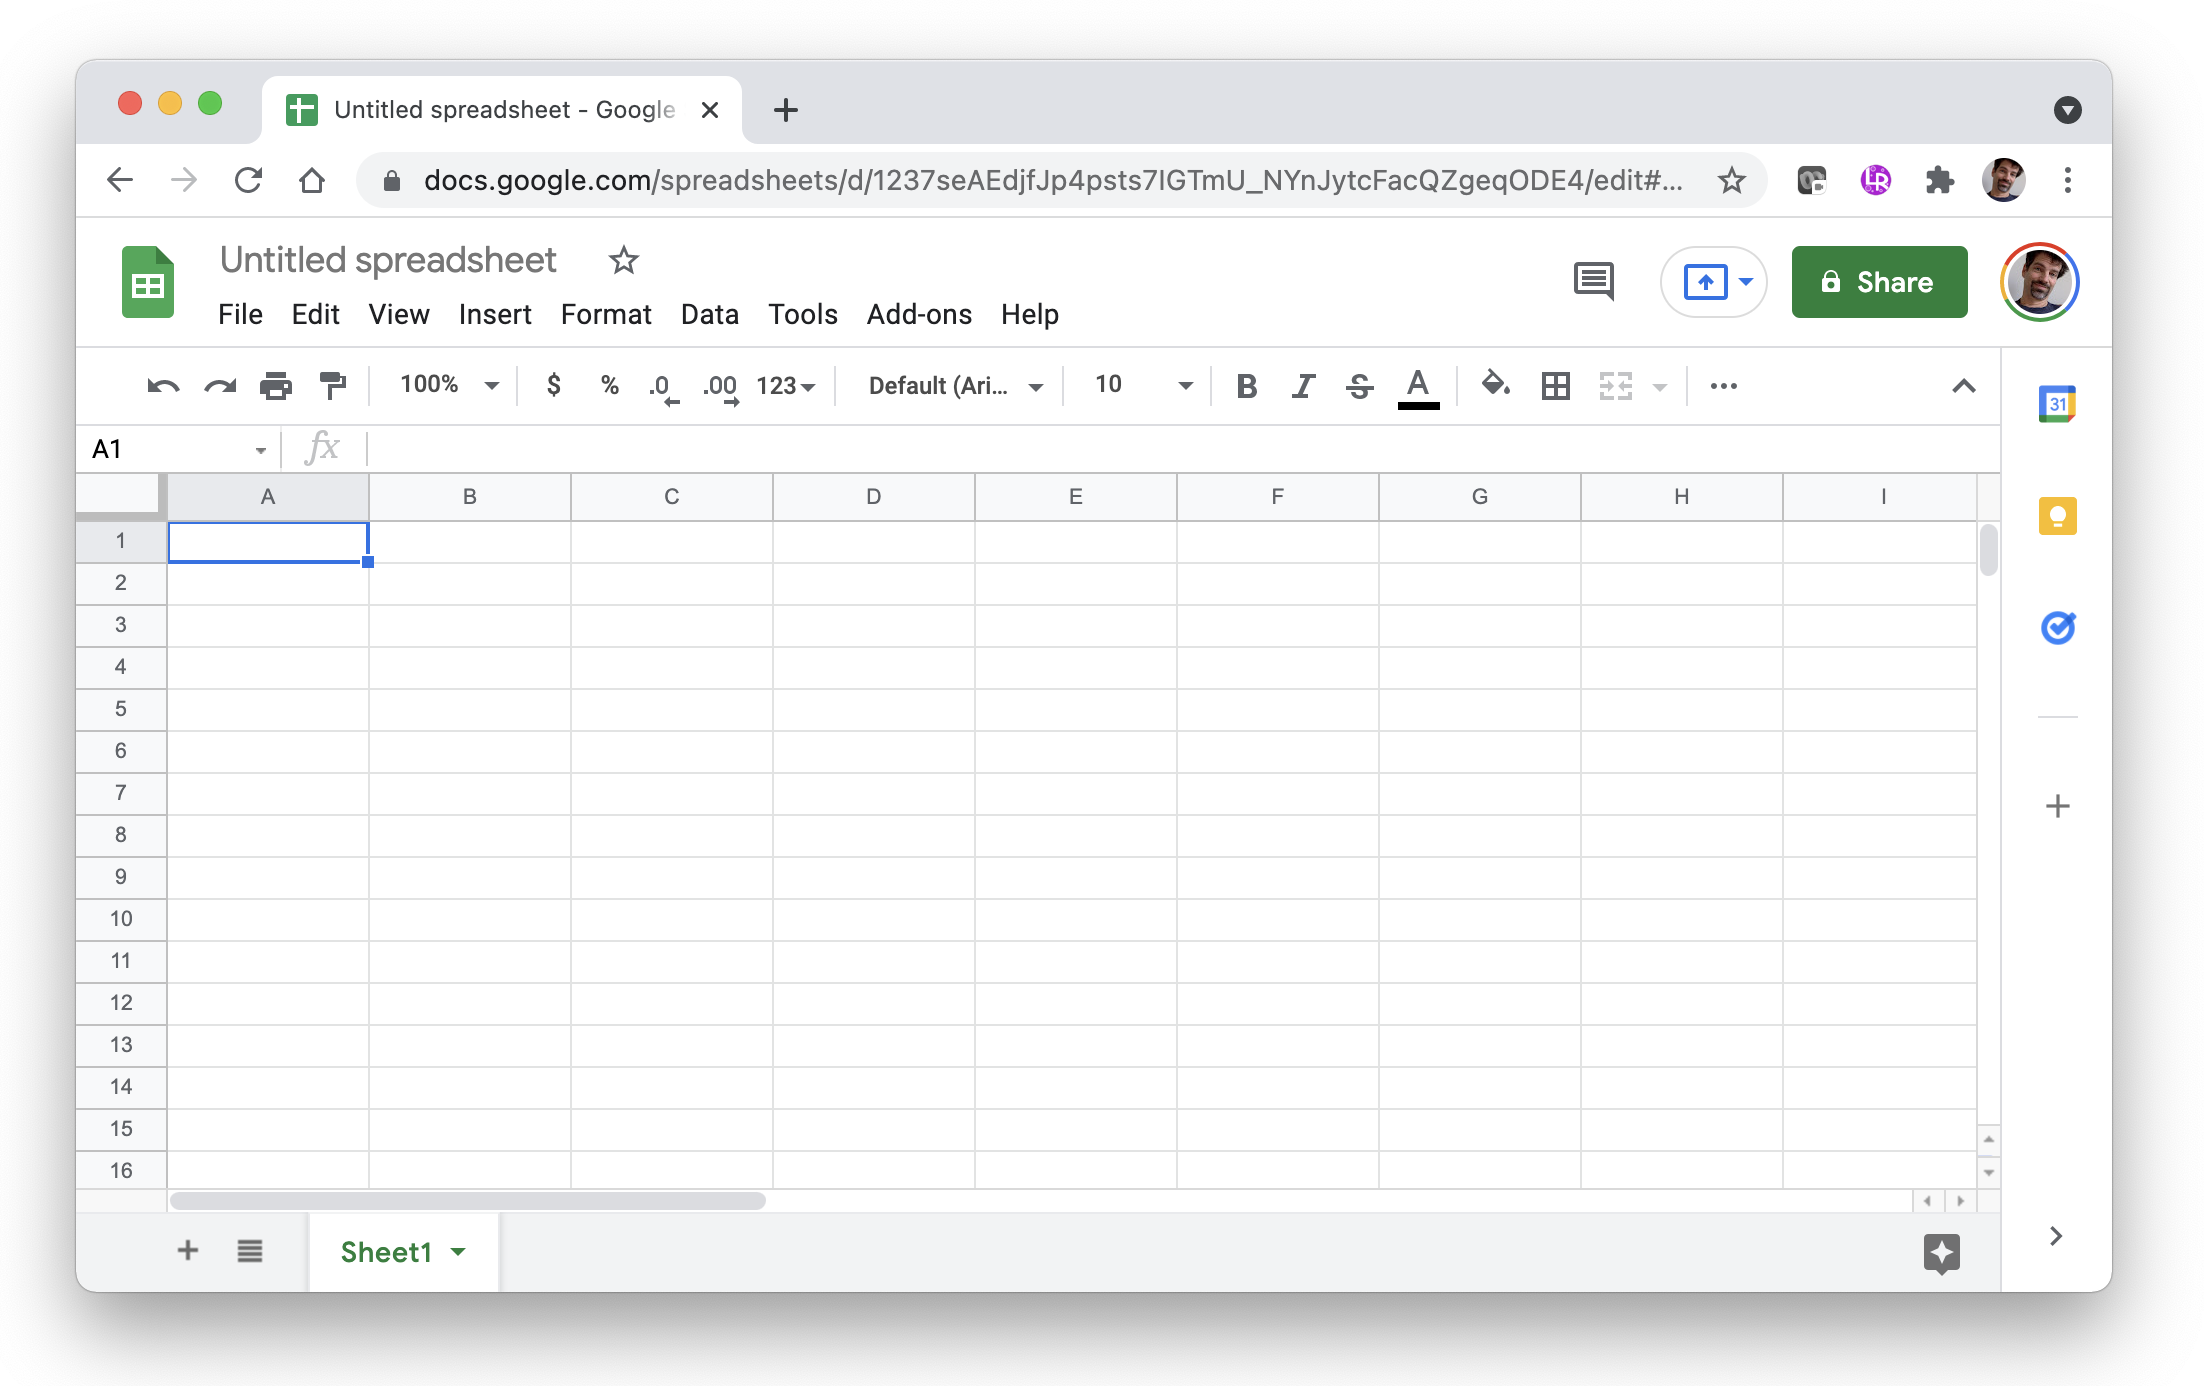
\includegraphics[width=0.6\textwidth]{BlankSheet.png}

Let's put some labels in the column:
\begin{itemize}
\item Select the first cell (A1) and type ``A number''.
\item Select the cell below it (A2) and type ``Another number''.
\item Select the cell below that one (A3) and type ``Their product''.
\item In the next column, type the number 5 in B1 and 7 in B2.
\end{itemize}

It should look like this:

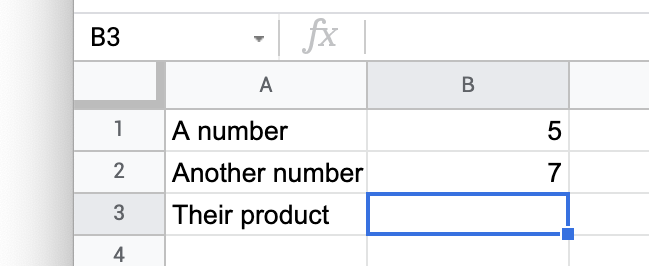
\includegraphics[width=0.5\textwidth]{NoFormulas.png}

Now put a formula in cell B3. Select B3, and type ``= B1 + B2''. The spreadsheet knows this is a formula because it starts with `=`. It will look like this as you type:\index{Spreadsheet!Entering formula}

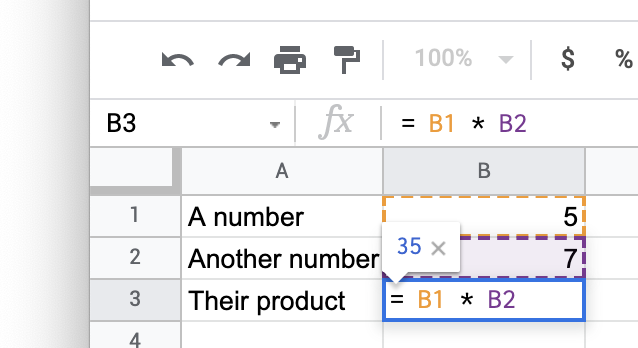
\includegraphics[width=0.5\textwidth]{TypingFirstFormula.png}

When you press Return or Tab, the spreadsheet will remember the formula, but display its value:

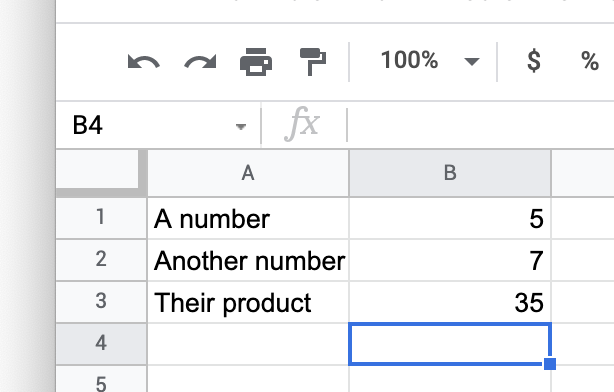
\includegraphics[width=0.5\textwidth]{FirstCalc.png}

If you change the values of cell B1 or B2, the cell B3 will automatically be recalculated. Try it.

\section{Formatting}

Every spreadsheet lets you change the formatting of your columns and cells. They are all a little different, so play with your spreadsheet a little now. Try to do the following:
\begin{itemize}
\item Set the background of the first column to light gray.
\item Right-justify the text in the first column.
\item Make the text in the first column bold.
\item Make the numbers in the second column have one digit after the decimal point.
\end{itemize}

It should look something like this:

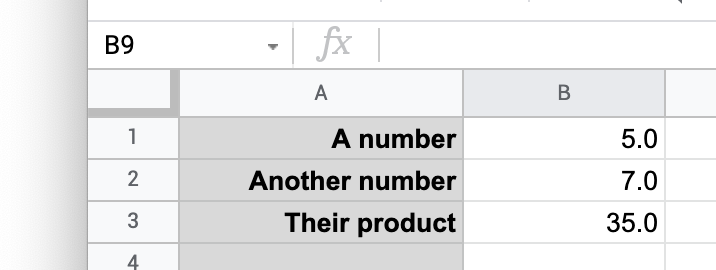
\includegraphics[width=0.6\textwidth]{FirstFormatting.png}

That's a spreadsheet. You have a grid of cells. Each cell can hold a
value or a formula that uses values from other cells. The cells with
formulas automatically update as you edit the values in the other
cells.

\section{Comma-Separated Values}

A lot of data is exchanged in a file format called
\textit{Comma-Separated Values} or just CSV. Each CSV file holds one
table of data. It is a text file, and each line of text corresponds to
one row of data in the table. The data in each column is separated by
a comma. The first line of a CSV is usually the names of the
columns. A CSV might look like this:

\begin{Verbatim}
studentID,firstName,lastName,height,weight
1,Marvin,Sumner,260,45.3
2,Lucy,Harris,242,42.2
3,James,Boyd,261,44.2
\end{Verbatim}

In your digital resources for this module, you should have a file
called \path{1000cars.csv}. It is a CSV with only one column called
``speed''. The first few lines look like this:

\begin{Verbatim}
speed
33.8000
29.9920
34.8699
27.9936
\end{Verbatim}

There is a title line and 1000 data lines.

Import this CSV into your spreadsheet program. In Google Sheets, it looks like this:

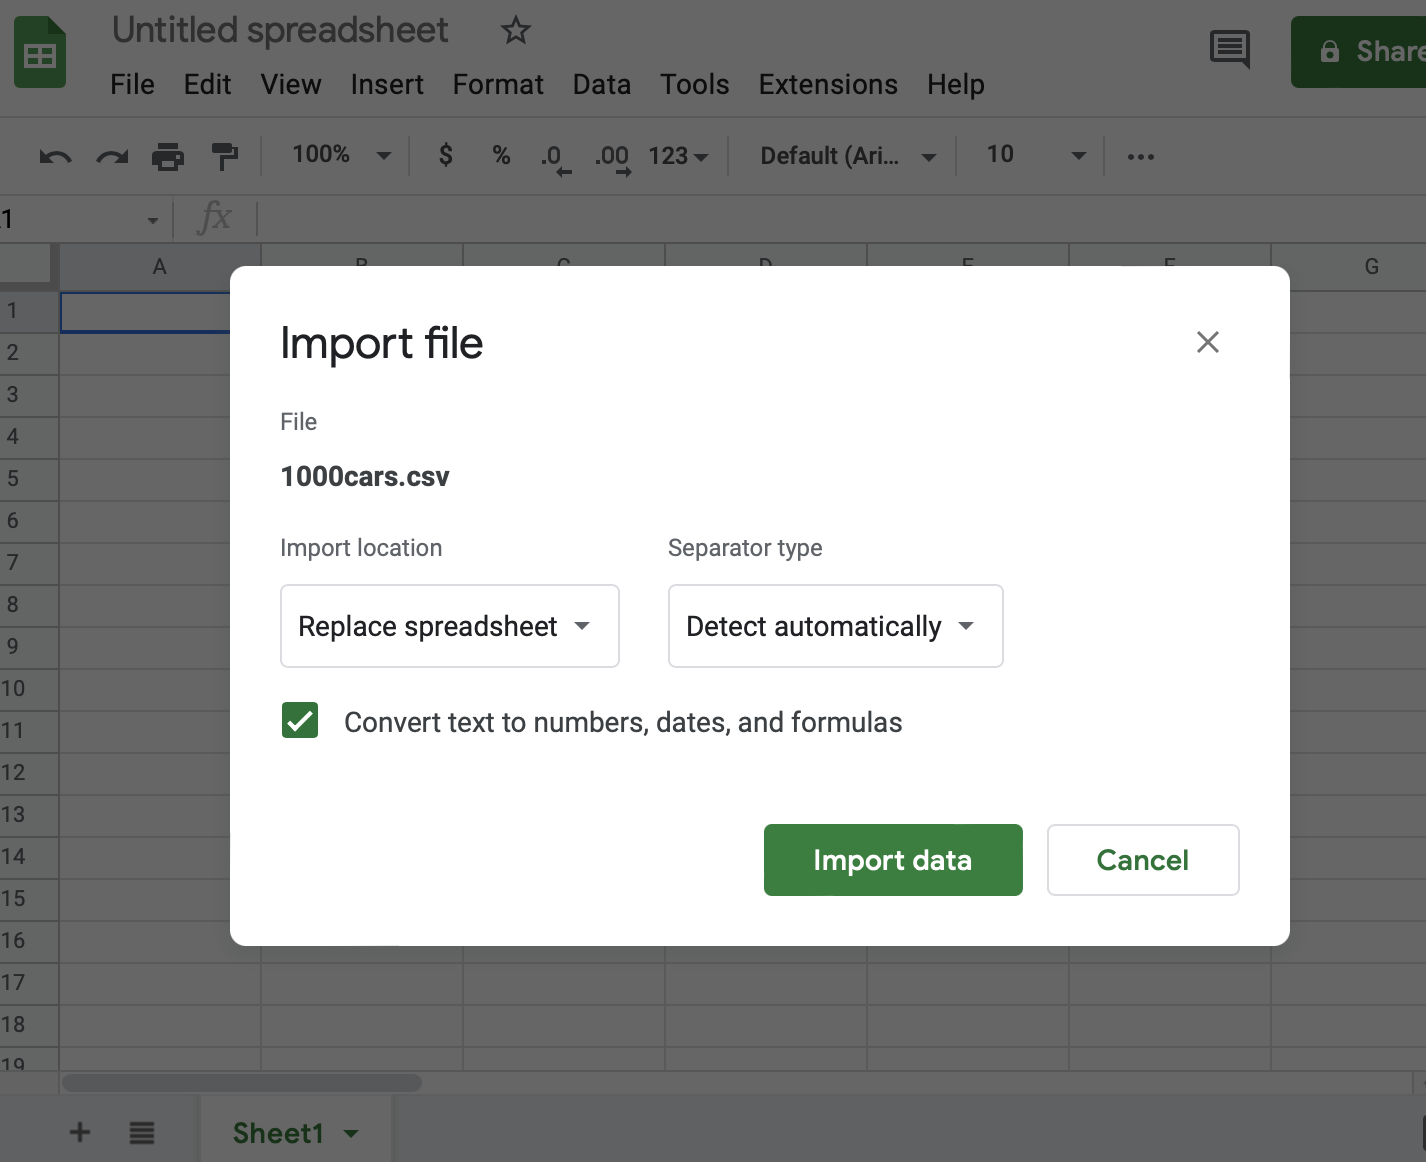
\includegraphics[width=0.5\textwidth]{ImportingCSV.png}

You should see a long, long column of data appear. (Mine goes from cell A2 through A1001.)

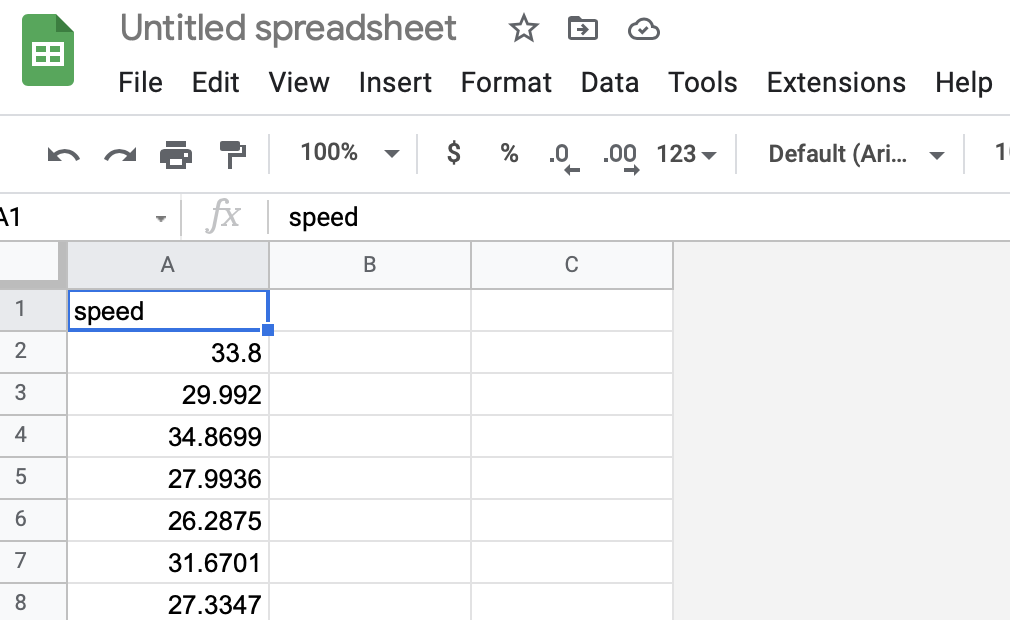
\includegraphics[width=0.5\textwidth]{ImportedCSV.png}

\section{Statistics in Spreadsheets}

Let's take the mean of all 1000 numbers.  In cell B2, type in a label:
``Mean''. (Feel free to format your labels as you wish. Bolding is recommended.)

In cell C2, enter the formula ``=AVERAGE(A2:A1001)''. When
you press return, the cell will show the mean: 31.70441, if done correctly.

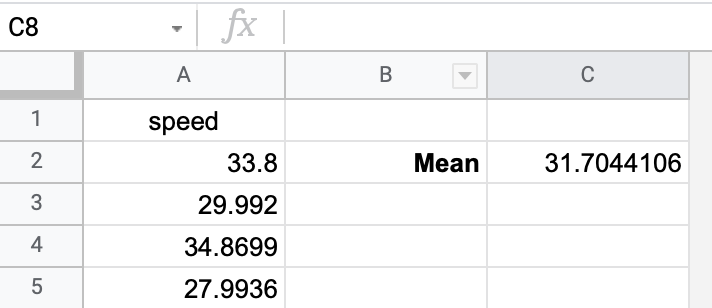
\includegraphics[width=0.4\textwidth]{Spread_mean.png}

Notice that by specifying that the function \pyfunction{AVERAGE} was to
be performed on a range of cells: cells A2 through A1001.

Do the calculations for variance, standard deviation, and median.

\begin{itemize}
\item The function for variance is \pyfunction{VAR}.
\item The function for standard deviation is \pyfunction{STDEV}.
\item The function for median is \pyfunction{MEDIAN}.
\end{itemize}

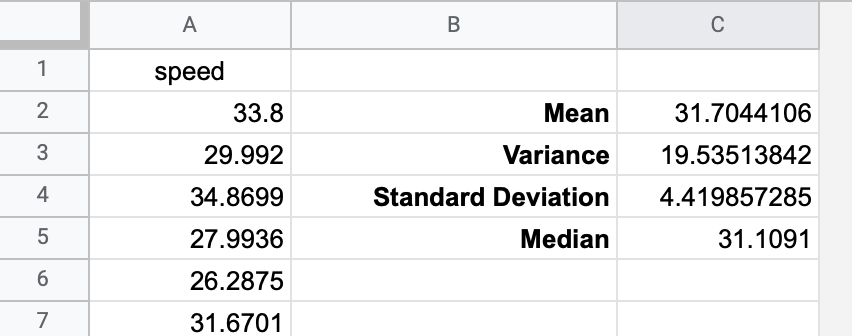
\includegraphics[width=0.4\textwidth]{var_stdev_median.png}

\section{Histogram}

Most spreadsheets have the ability to create a histogram. In Google
Sheets, you select the entire range A2:A1001 by selecting the first
cell and then shift-clicking the last. Then you choose
Insert$\rightarrow$Chart. In the inspector, change the type of the
chart to a histogram. This will get you a basic histogram.
% Add: Define histogram or give example, defined in basic statistics, must come previous

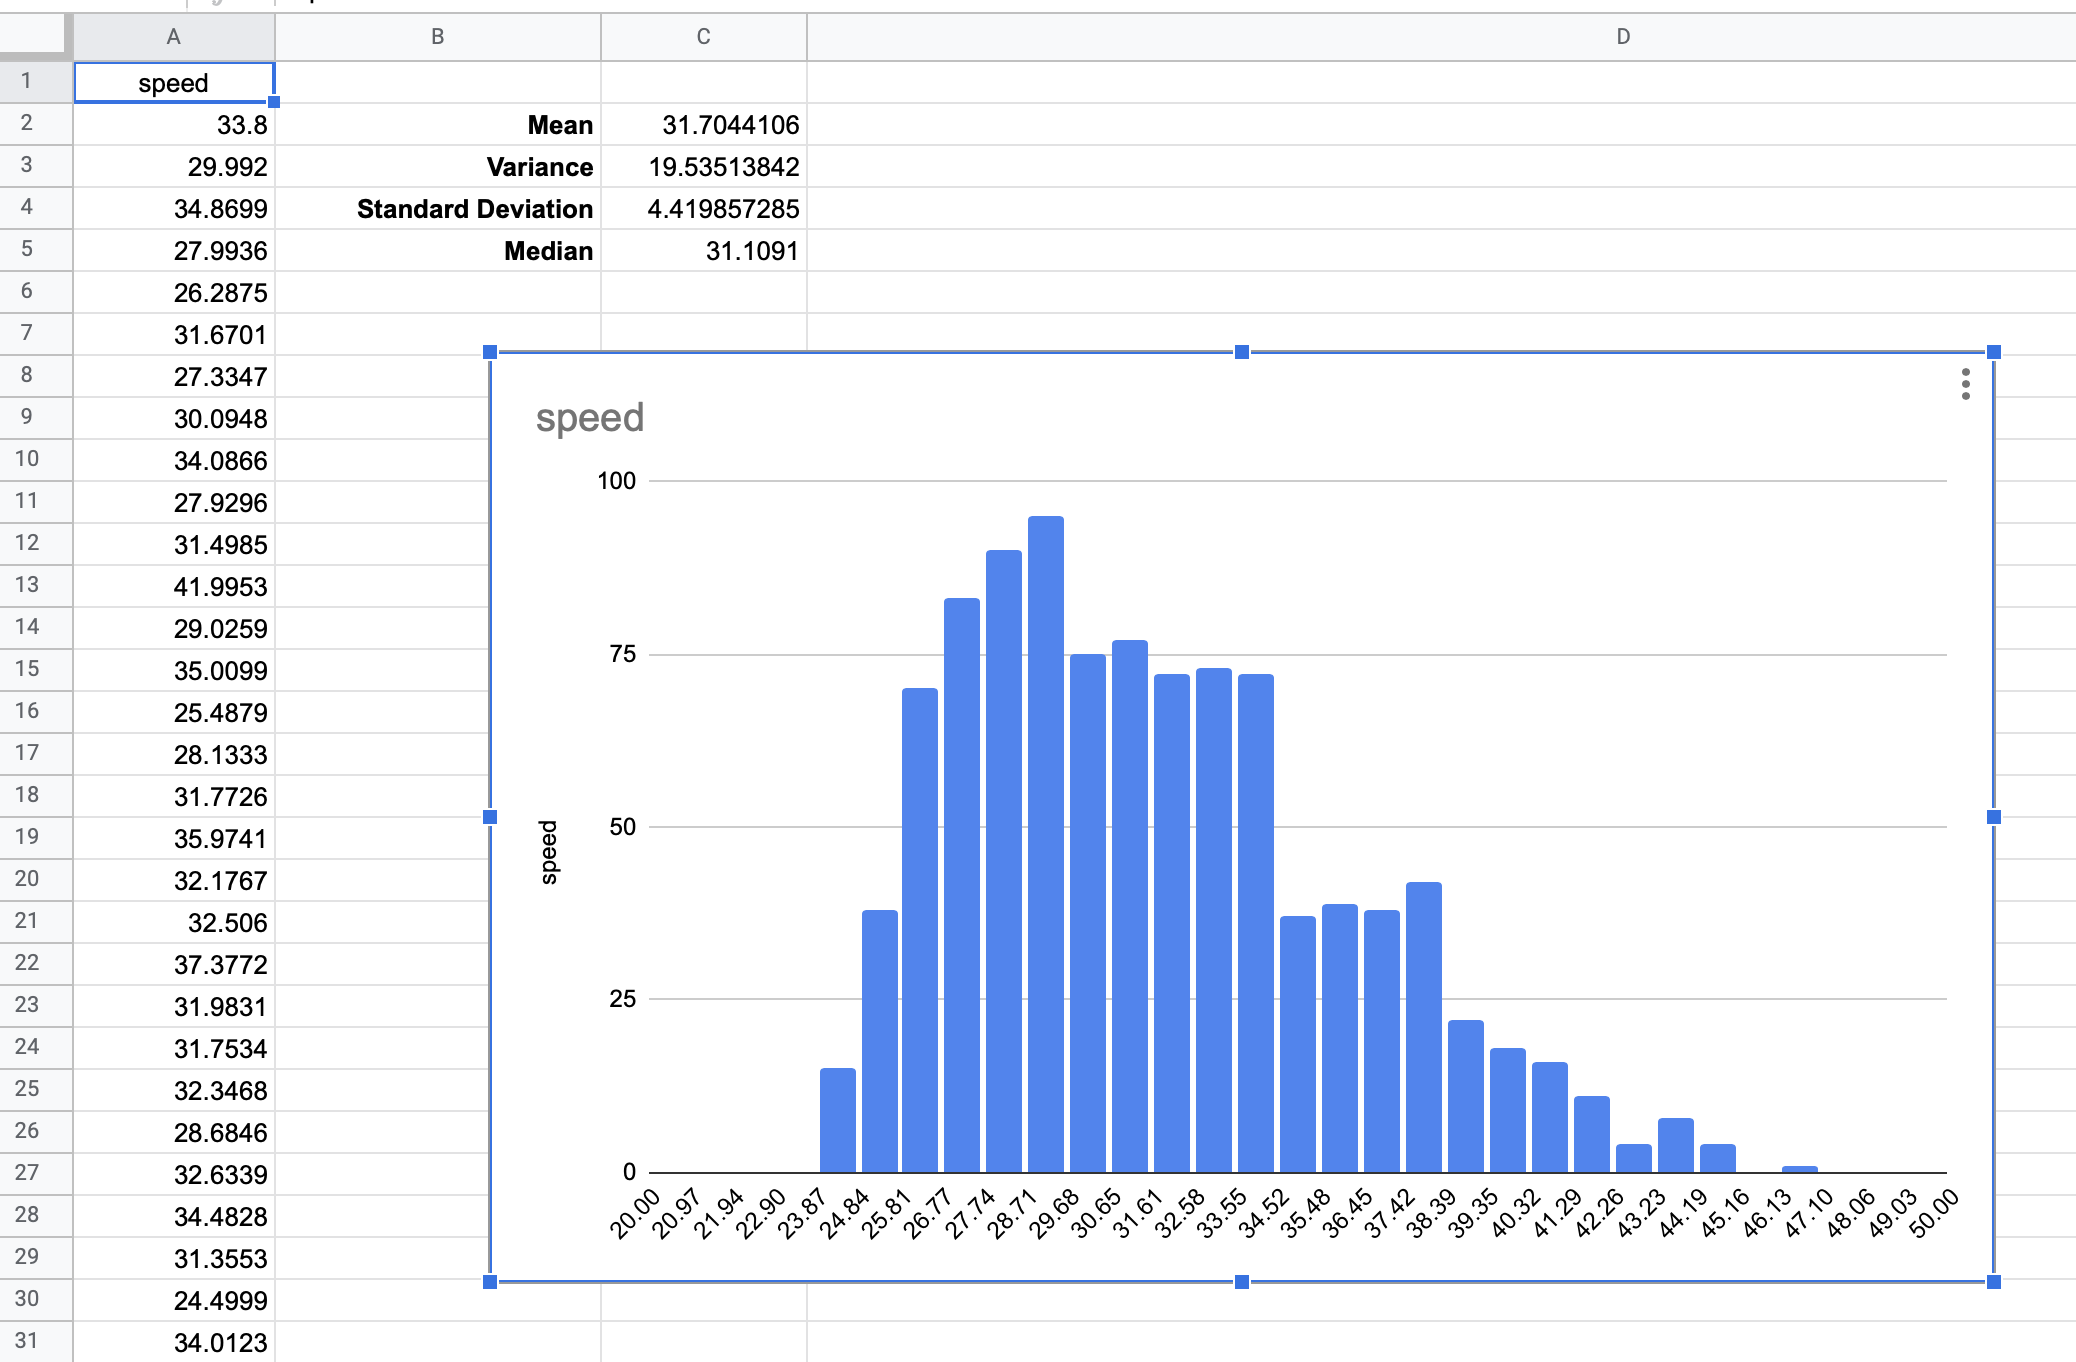
\includegraphics[width=0.7\textwidth]{default_histogram.png}

Play with the formatting to see how unique you can make data. Here is an example:

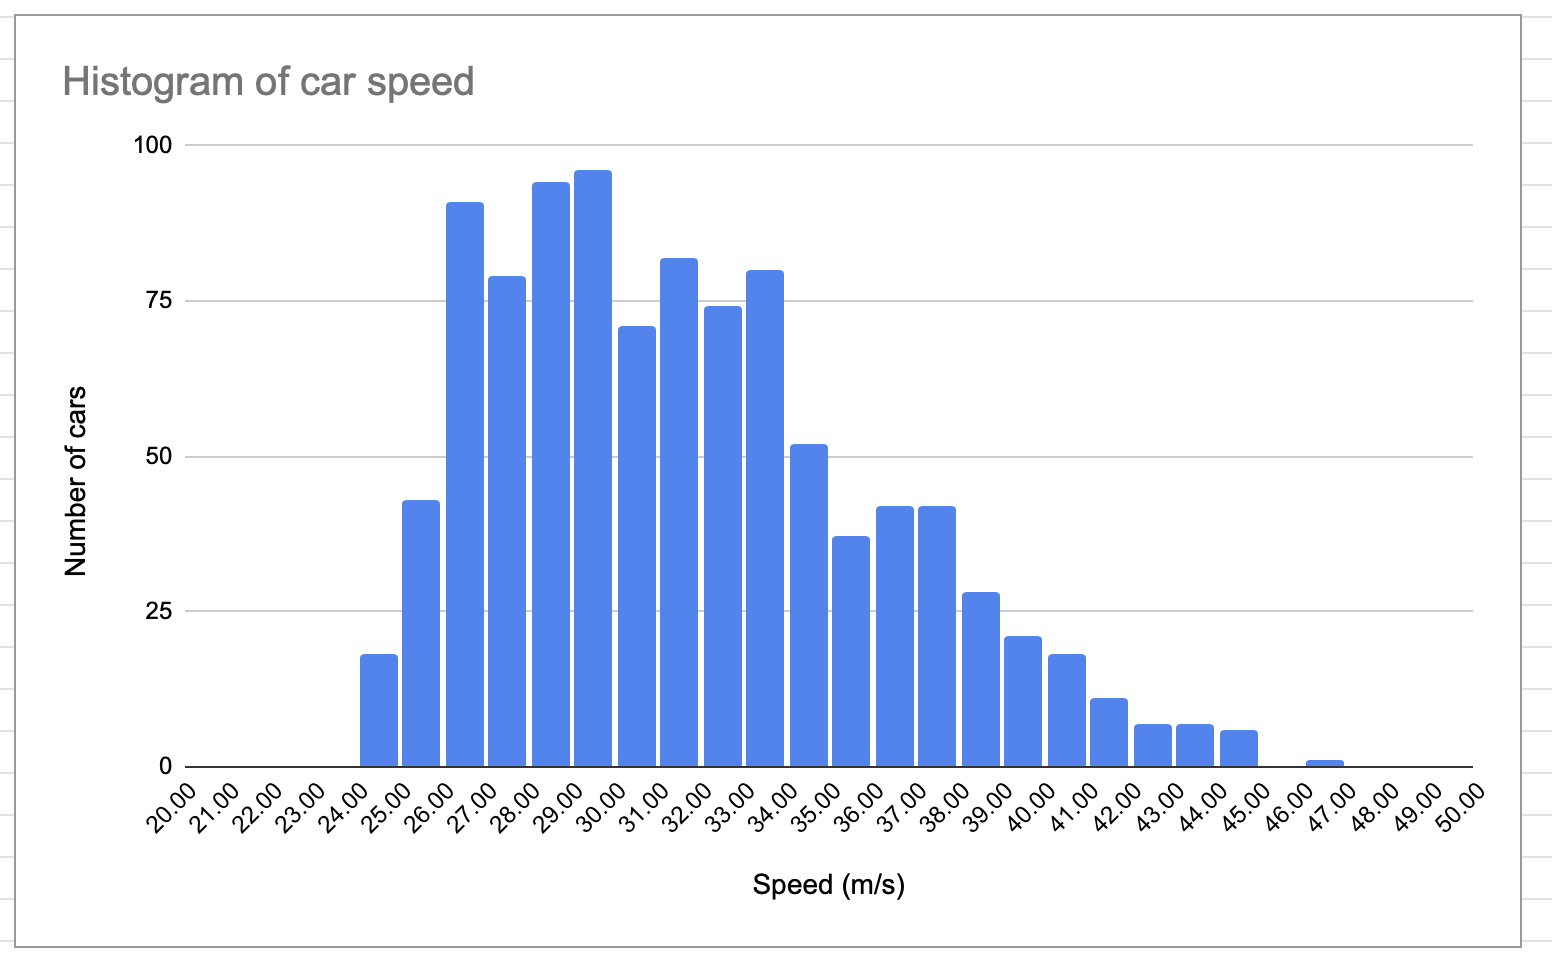
\includegraphics[width=0.8\textwidth]{final_histogram.png}

\begin{Exercise}[title={RMS}, label=rms_spreadsheet]

  In your spreadsheet, calculate the quadratic mean (the root-mean-squared) of the speeds.

  You will need the following three functions:
  \begin{itemize}
  \item \pyfunction{SUMSQ} returns the sum of the squares of a range of cells.
  \item \pyfunction{COUNT} returns the number of cells in a range that contains numbers.
  \item \pyfunction{SQRT} returns the square root of a number.
  \end{itemize}


\end{Exercise}
\begin{Answer}[ref=rms_spreadsheet]

The formula for the RMS is ``=SQRT(SUMSQ(A2:A1001)/COUNT(A2:A1001))''.
% KA: https://www.khanacademy.org/computing/ap-computer-science-principles/data-analysis-101/data-tools/a/learning-from-data-sets

\end{Answer}


\graphicspath{{../../Chapters/dc1/en_US}}
\chapter{Introduction to Electricity}

What happens when you turn on a flashlight? The battery in the
flashlight acts as an electron pump. The electrons flow through the
wires to the lightbulb (or LED). As the electrons pass through the
lightbulb, they excite the molecules within, which gives off light and
heat. (LEDs also give off light and heat, but they give off a lot less
heat.) Then the electrons return to the battery to be pumped around
again.

When electricity is flowing through a copper wire, the protons and
neutrons of the copper stay put while the electrons jump between the
atoms on their way from the battery to the lightbulb and back again.

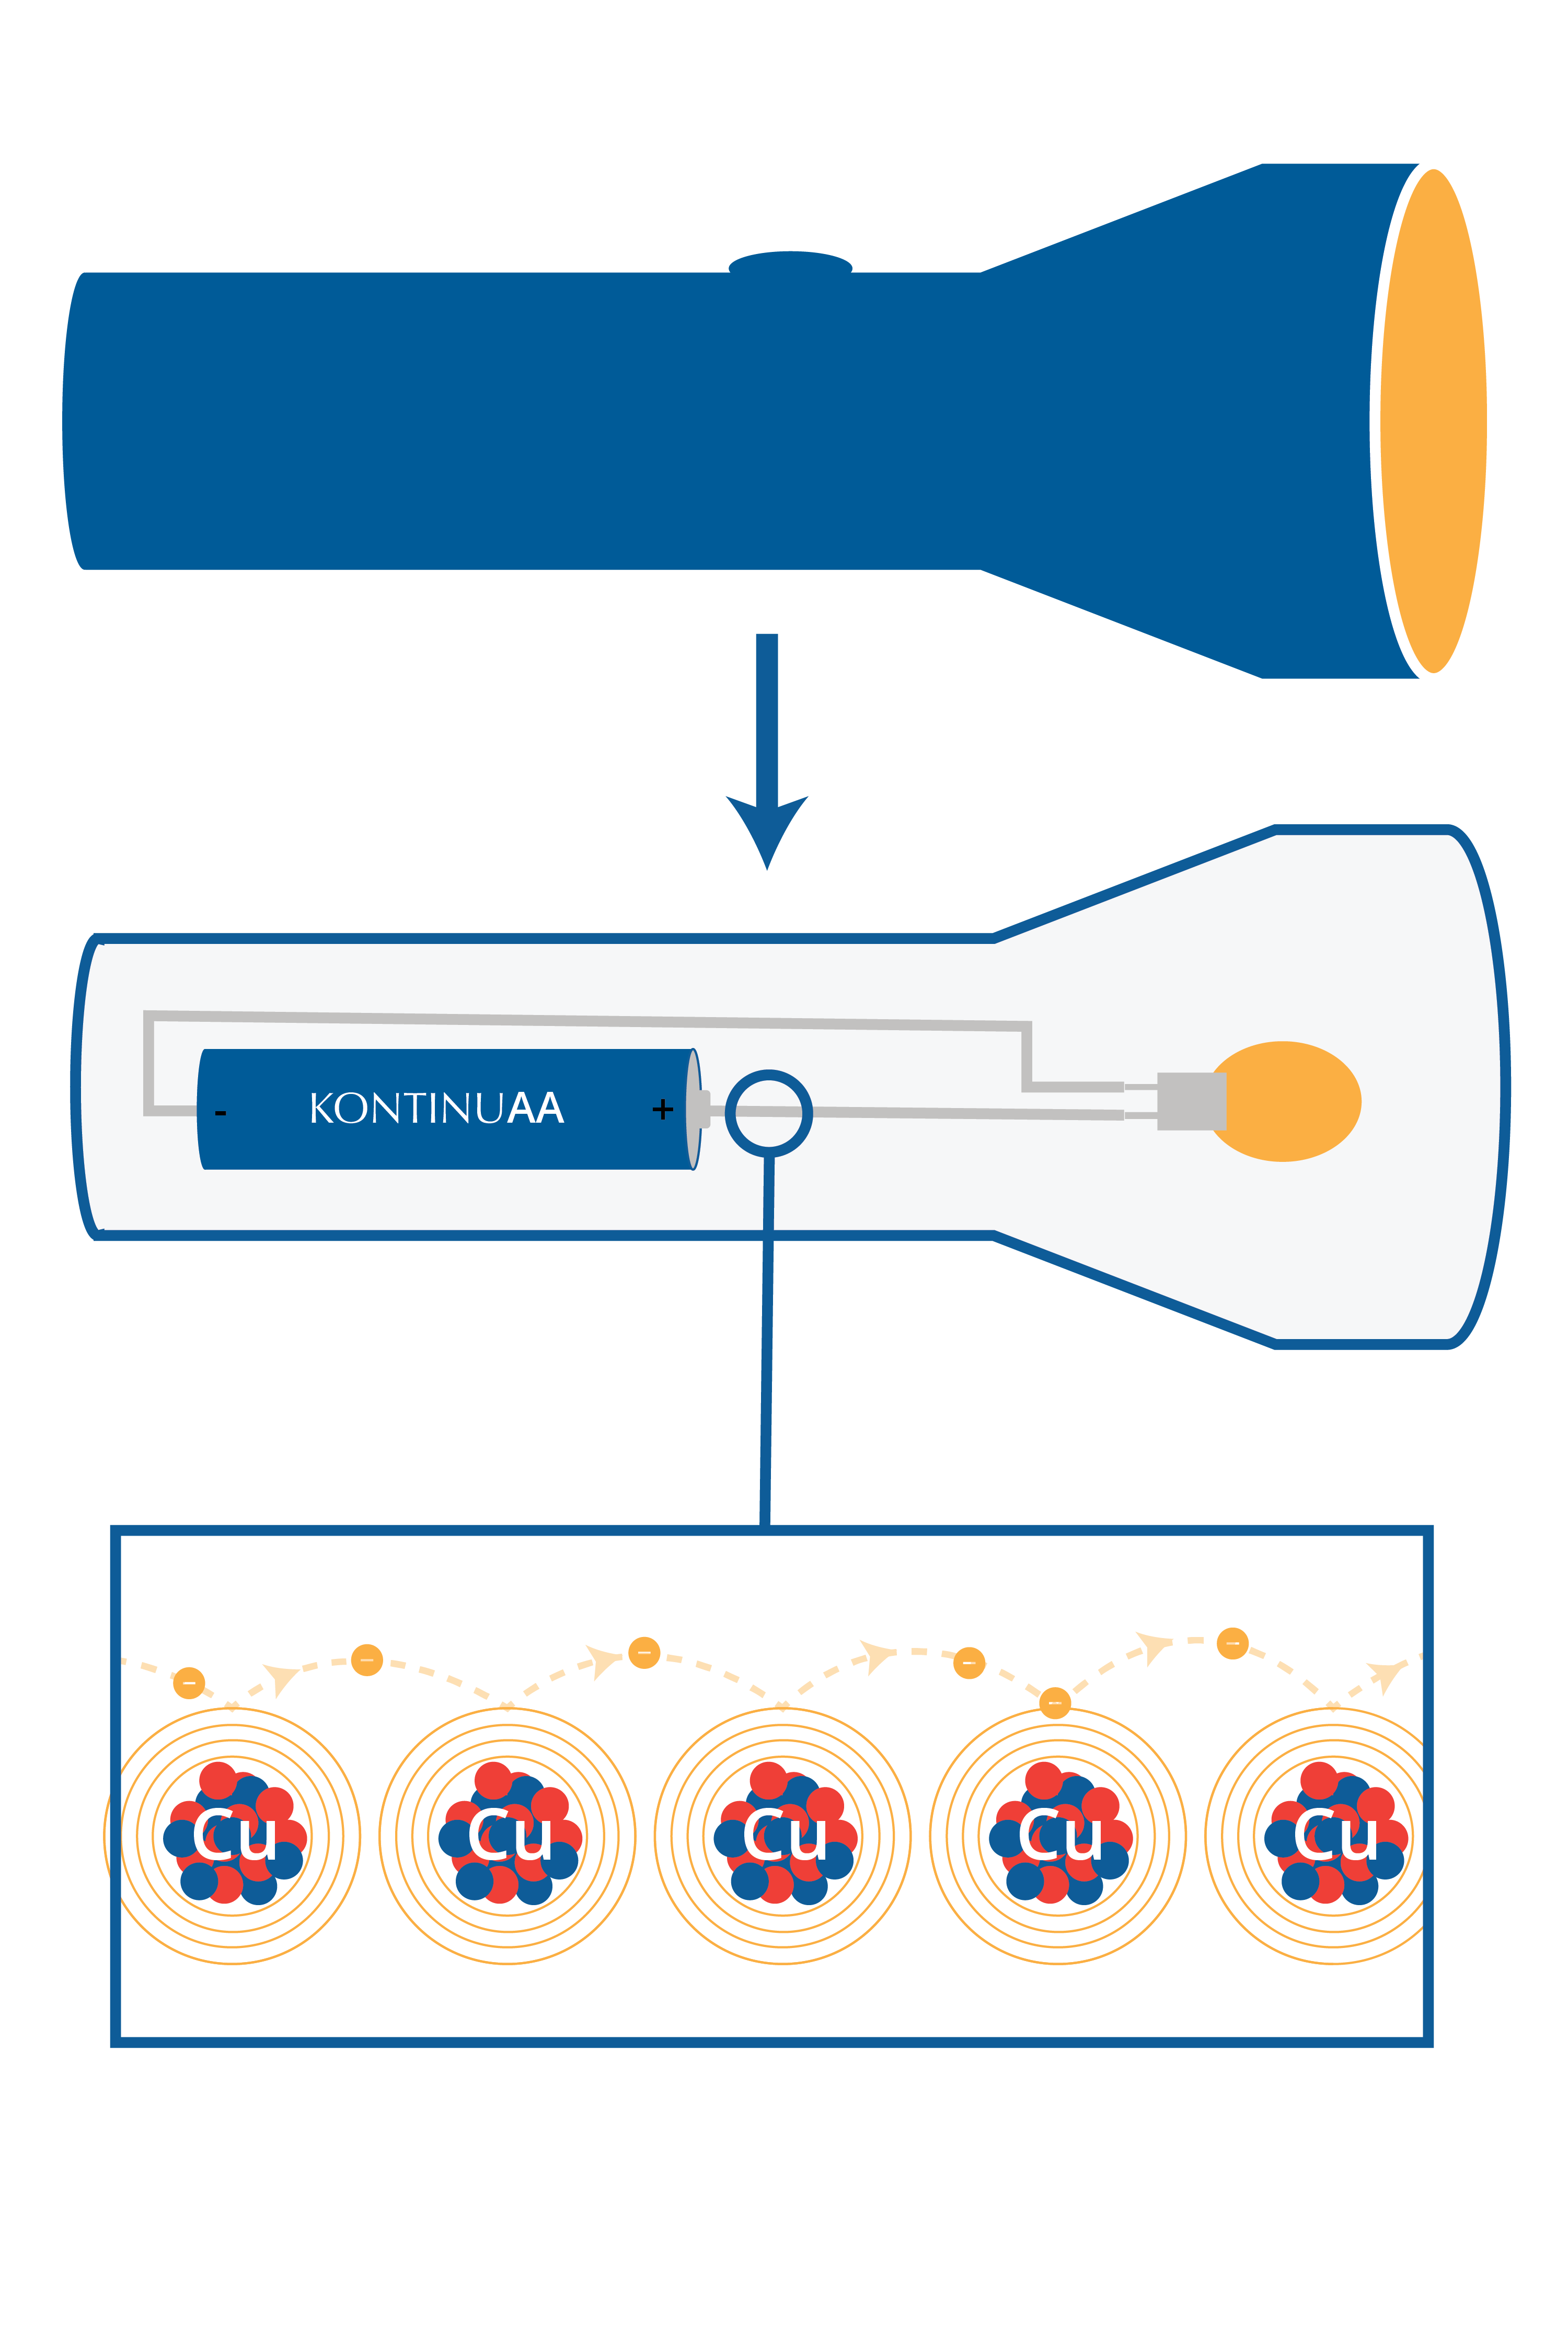
\includegraphics[width=.5\textwidth]{flashlight.png}


In some materials, like copper and iron, electrons are loosely bound
to their nuclei, forming a sea of electrons, which allows energy to flow. These are good \textit{electrical conductors}. In
other materials, like glass and plastic, electrons don't leave their
nuclei easily. Thus, they are terrible electrical conductors -- we call
them \textit{electrical insulators}. For example, the plastic around a
wire is electrical insulation.

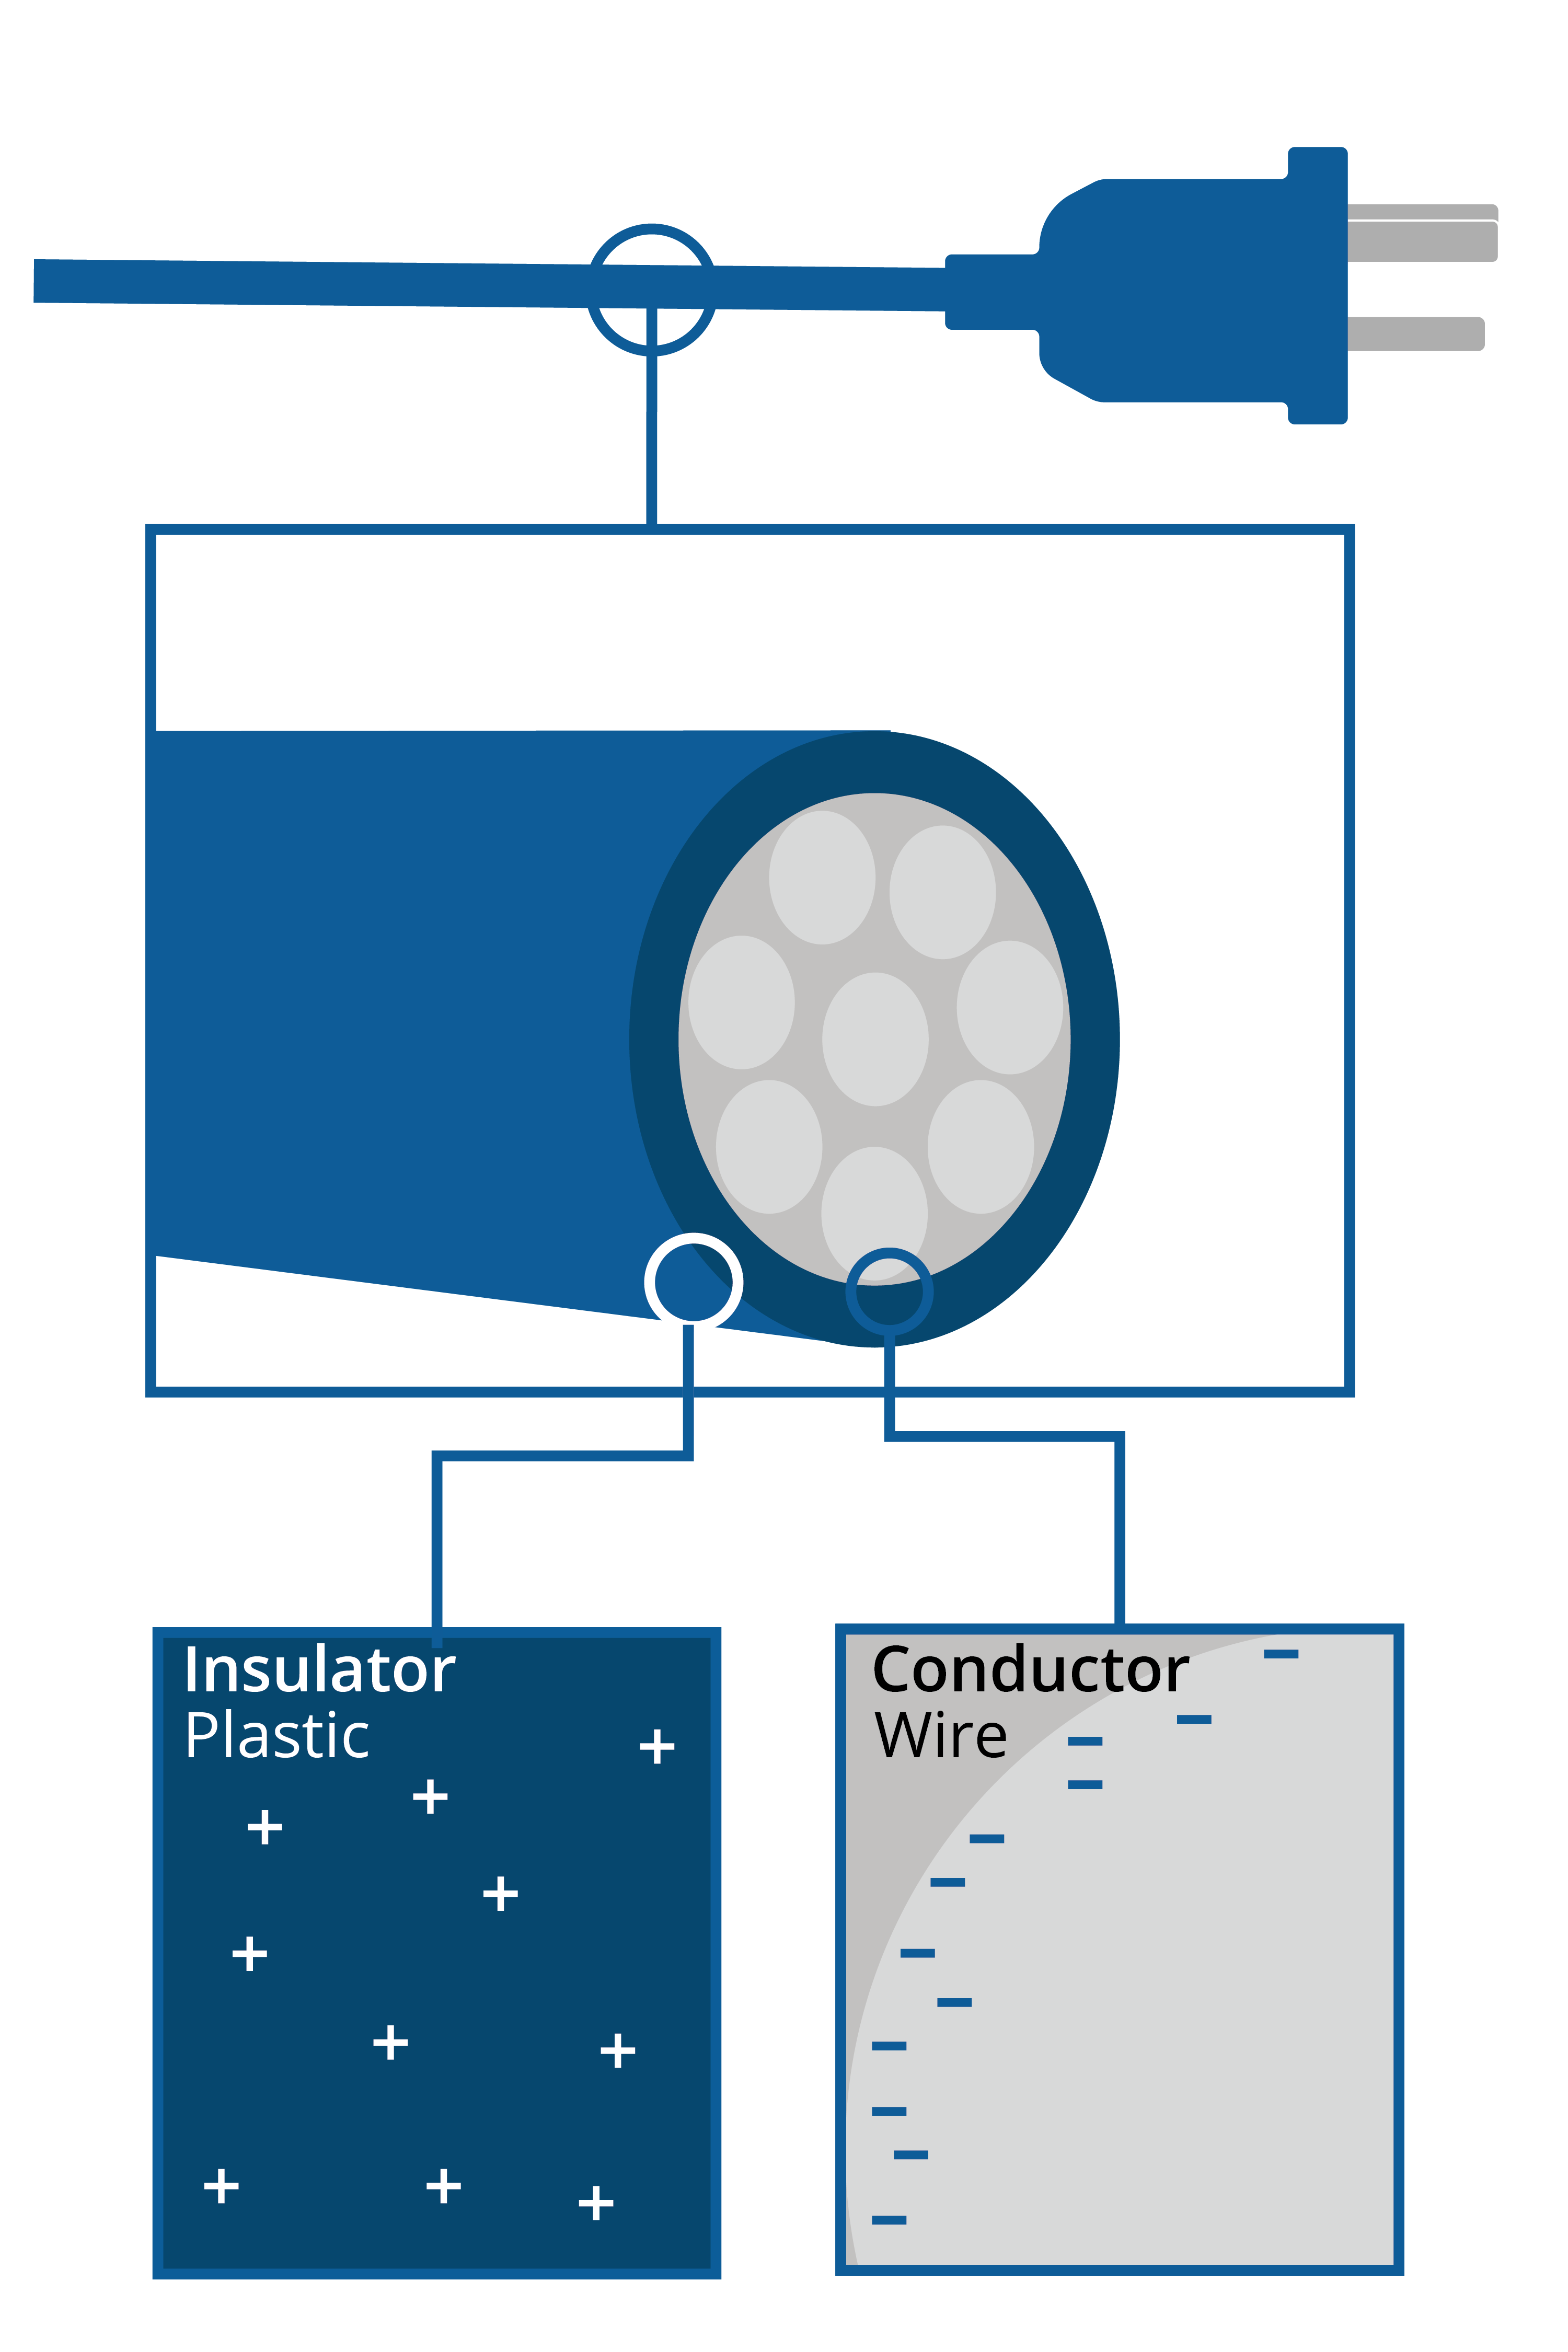
\includegraphics[width=.8\textwidth]{plug.png}

% KA: https://www.khanacademy.org/science/physics/electric-charge-electric-force-and-voltage/charge-electric-force/v/conductors-and-insulators

\section{Units}

Electrons are very small, so to study them, scientists came up with a
unit that represents \textit{a lot} of electrons. 1 \textit{coulomb}
is about 6,241,509,074,460,762,608 electrons.  When 5 coulombs enter one end of the wire every second (and simultaneously 5 coulombs exit the other end), we say ``This wire is carrying 5 amperes of current.''\index{coulombs}

(Truthfully, we usually shorten ampere to just ``amp''.  This is
sometimes a little awkward because we often shorten the word
``amplifier'' to ``amp''. You should be able to tell which is which
from the context.)\index{amp or ampere}

If you look at the circuit breakers or fuses for your home's
electrical system, you'll see that each one is rated in amps.  For
example, maybe the circuit that supplies power to your kitchen has a 10
amp circuit breaker. If for some reason, more than 10 amps tries to
pass through that wire, the circuit breaker will turn off the whole
circuit.

When it is on, your flashlight pushes about 1 amp of current
through the lightbulb(When it is off, there is no current in the
lightbulb).

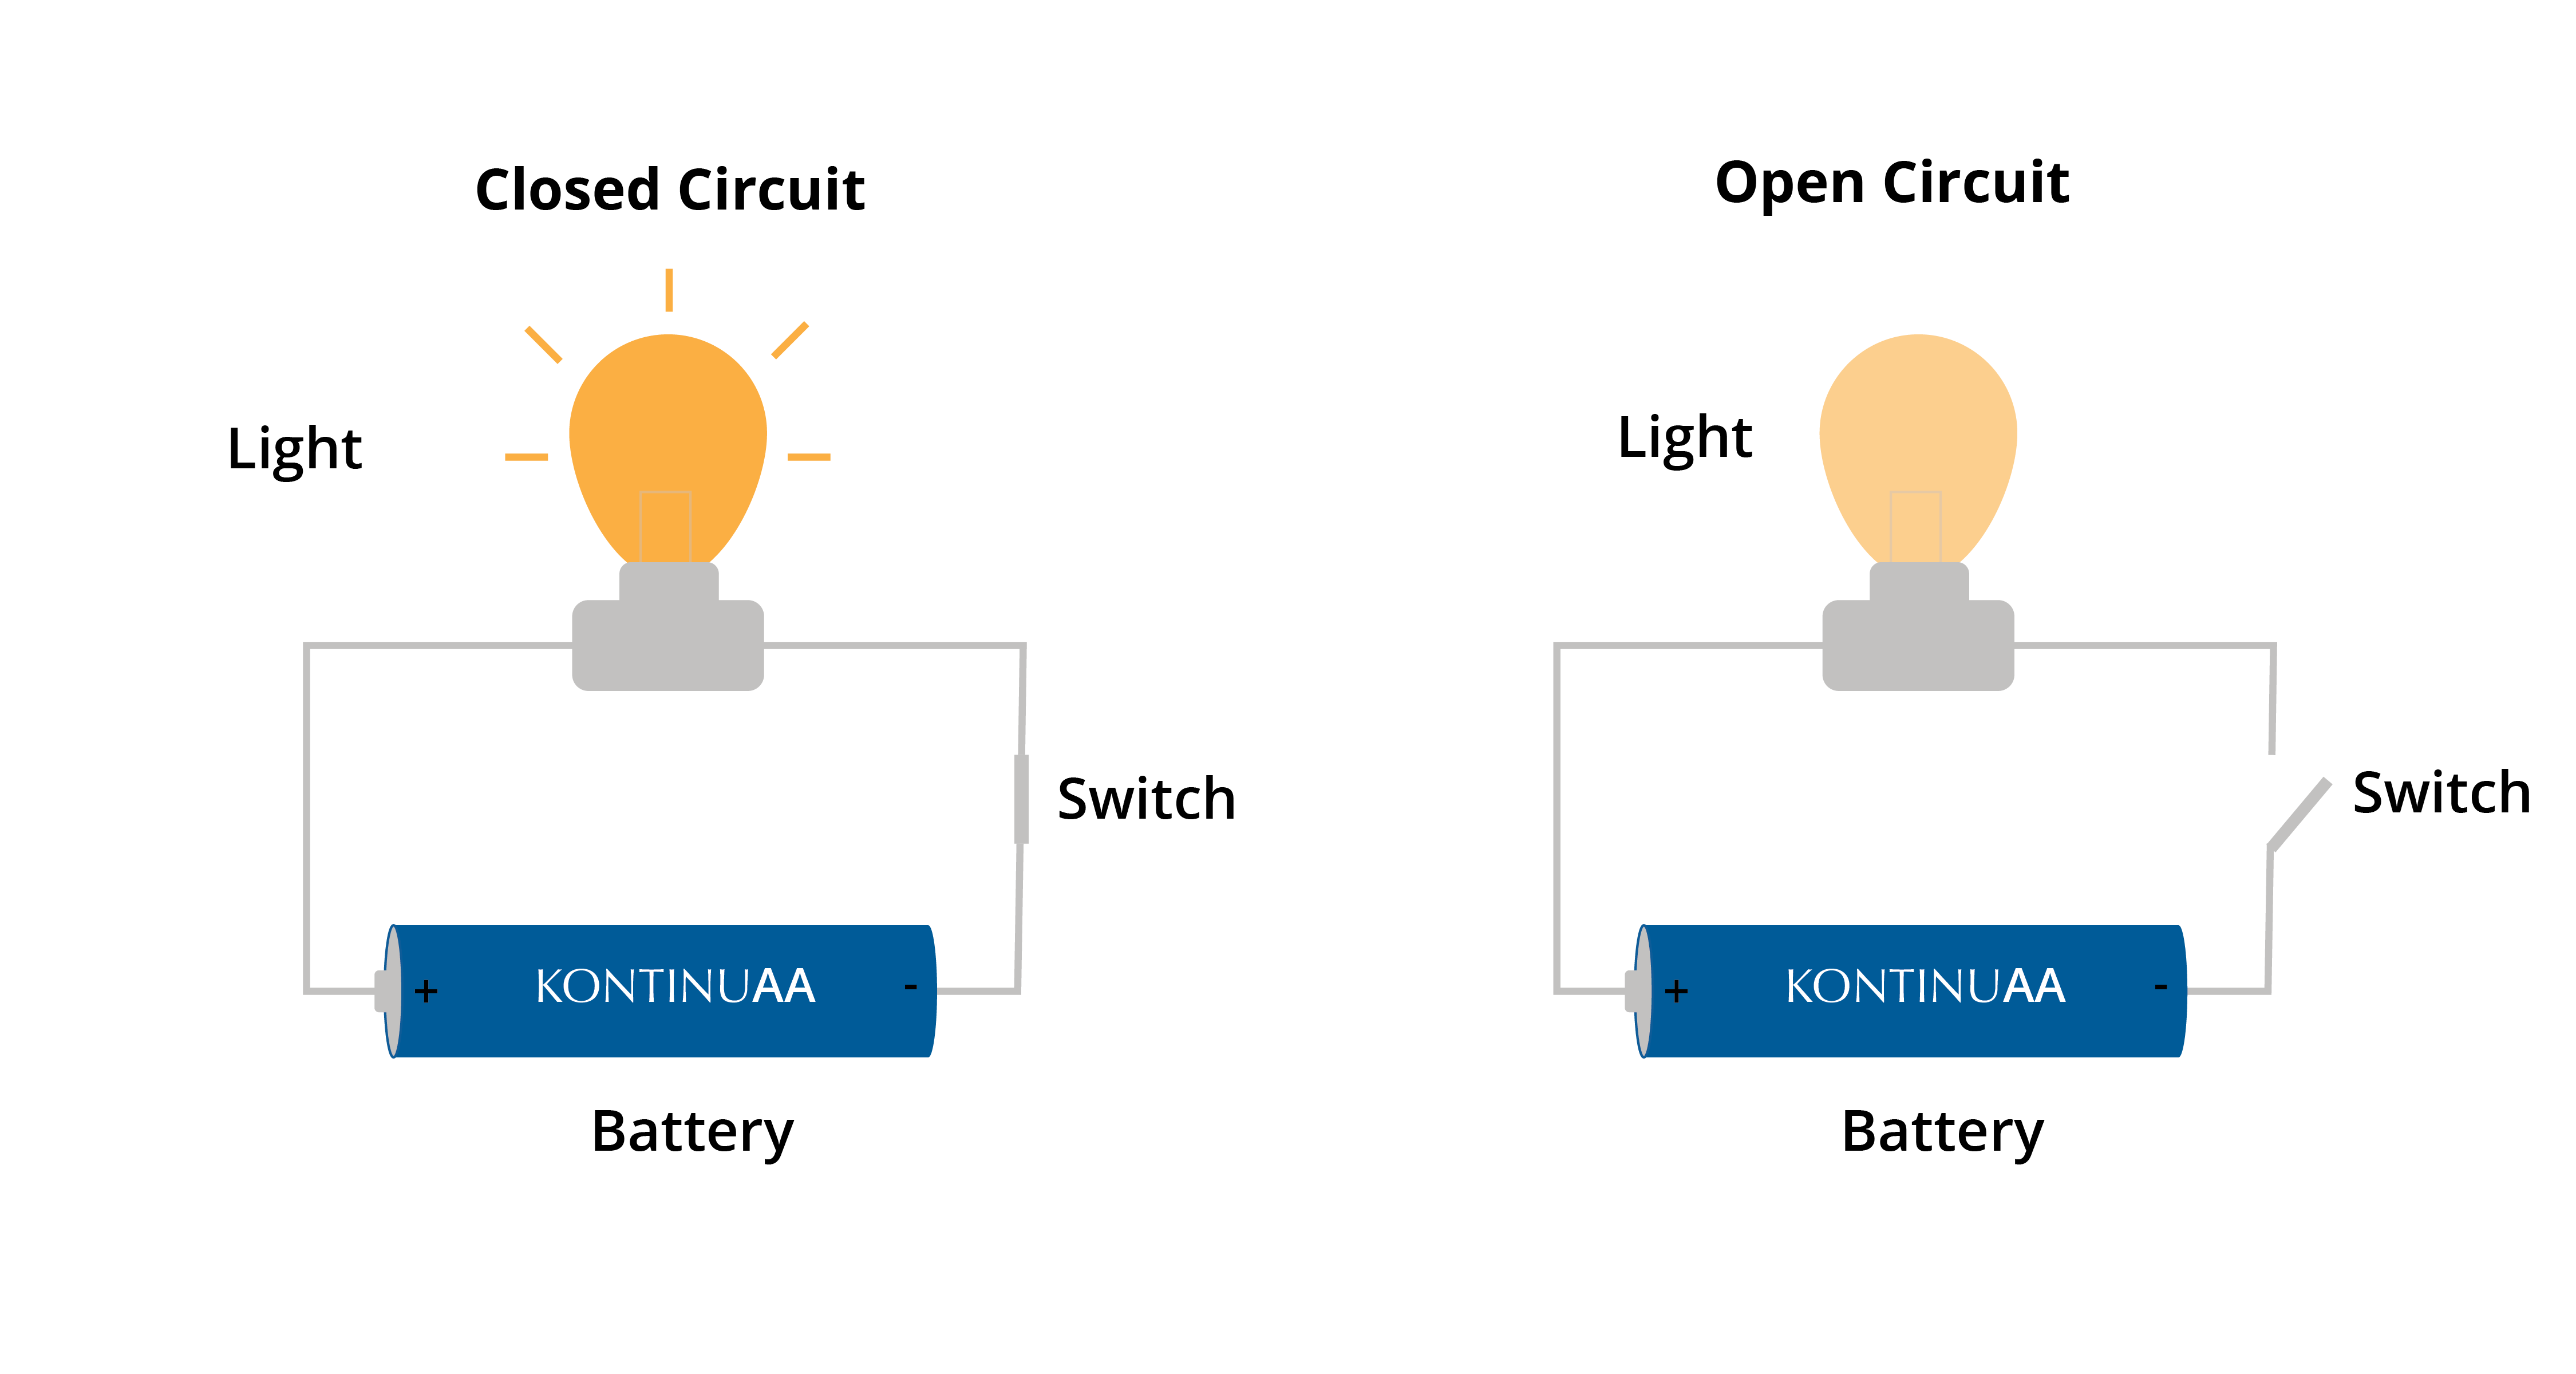
\includegraphics[width=0.8\textwidth]{Circuit_OnOff.png}

The lightbulb creates \textit{Resistance} that the current pushes
through.\index{resistance} Think of it like plumbing: The current is the amount of water
passing through a pipe. The resistance is something that tries to stop
the current -- like a ball of hair. The battery is what allows
 the current to push through the resistance; we call that
pressure \textit{voltage}.\index{voltage}

\section{Circuit Diagrams}

Here is a circuit diagram of your flashlight:

\begin{circuitikz}
\draw (0,0) to[battery1,invert,l=$3V$] ++(0,3)
to [switch,i=1A] ++(3,0)
to [lamp=$1\Omega$,bipoles/length=0.9cm] ++(0,-3) -- (0,0);
\end{circuitikz}

The lines are wires.  The symbols that we  will use:

\begin{tabular}{c c c c}
  Battery & Switch & Lamp & Resistor \\
\begin{circuitikz}
\draw (0,0) to[battery1] (2,0); 
\end{circuitikz}
&
\begin{circuitikz}
\draw (0,0) to[lamp,bipoles/length=0.9cm,l=$3 \Omega$] (2,0); 
\end{circuitikz}
&
\begin{circuitikz}
\draw (0,0) to[switch,/tikz/circuitikz/bipoles/length=1.0cm] (2,0); 
\end{circuitikz}
&
\begin{circuitikz}
\draw (0,0) to[R,  l=$3 \Omega$] (2,0); 
\end{circuitikz} \\
\end{tabular}

The battery pushes the electrons from one end and pulls them back in at the other, so the circuit must go around in a circle for the current to flow. This is why the current stops flowing when the switch breaks the circuit.

You can think of a switch as having zero resistance when it is closed and infinite resistance when it is open.


For our purposes, a lamp is just a resistor that gives off light.
% KA: https://www.khanacademy.org/science/high-school-physics/dc-circuits/electric-power-and-dc-circuits/a/circuit-introduction

\section{Ohm's Law}

Resistance is measured in \textit{ohms}, and we use a Greek capital omega for that: $\Omega$  

Voltage is measured in
\textit{volts}.\index{ohms}\index{volts}

\begin{mdframed}[style=important, frametitle={Ohm's Law}]\index{Ohm's law}
  Whenever a voltage $V$ is pushing a current $I$ through a resistance of $I$, the following is true:

  $$V = IR$$

  where $V$ is in volts, $I$ is in amps, and $R$ is in ohms.
\end{mdframed}
% KA: https://www.khanacademy.org/science/physics/circuits-topic/circuits-resistance/v/circuits-part-1

\section{Power and Watts}

\begin{mdframed}[style=important, frametitle={Joule's Law}]\index{Joule's law}

  When a current $I$ is passing through a resistance $R$, the power consumed is
  
  $$W = I^2 R$$

  where $W$ is in watts, $I$ is in amps, and $R$ is in ohms.
\end{mdframed}

Of course $V = IR$, so we can extend this to:

$$W = I^2 R = I V = \frac{V^2}{R}$$

Your flashlight's batteries provide about 3 volts. How much
battery power is the flashlight using when it is on? The power (in
watts) produced by the battery is the product of the voltage (in
volts) and the current (in amps). So your flashlight is giving off $3
volts \times 1 amp = 3 watts$ of power. Some of that power is given
off as light, some as heat.\index{watts}

A watt is 1 joule of energy per second. We say that a watt is a
measure of \textit{power}.

When we talk about how much energy is stored in a battery, we use a
unit like a kilowatt-hour. A kilowatt-hour is equivalent to 3.6 million
joules.

\section{Another great use of RMS}

In many electrical problems, the voltage fluctuates a lot.  For
example, the fluctuations in voltage makes the sound that comes out of an
audio speaker.

You can use the root-mean-squared of the voltage to figure out the average power
your speaker is consuming.

Let's say that the RMS of the voltage you are sending to the speaker is $V_{rms}$
and the resistance of the speaker is $R$ ohms, then the power consumed
by the speaker is:

$$P = \frac{V_{rms}^2}{R}$$

Similarly, if you know the RMS of the current you are pushing through
the speaker is $I_{rms}$, then the power consumed by the speaker is:

$$P = I_{rms} R$$

\section{Electricity Dangers}

Large amounts of electricity moving through your body can hurt or even kill
you. You must be careful around electricity.

However, your body is not a very good conductor, so low-voltage
systems (like a flashlight) don't have enough voltage to move significant amounts of
current through your body.

However, the  electricity in a power outlet has much more voltage. The voltage
in these outlets is fluctuating between positive and negative, so we
call it \textit{Alternating Current} or AC.
% ADD: Introduce difference between AC and dc

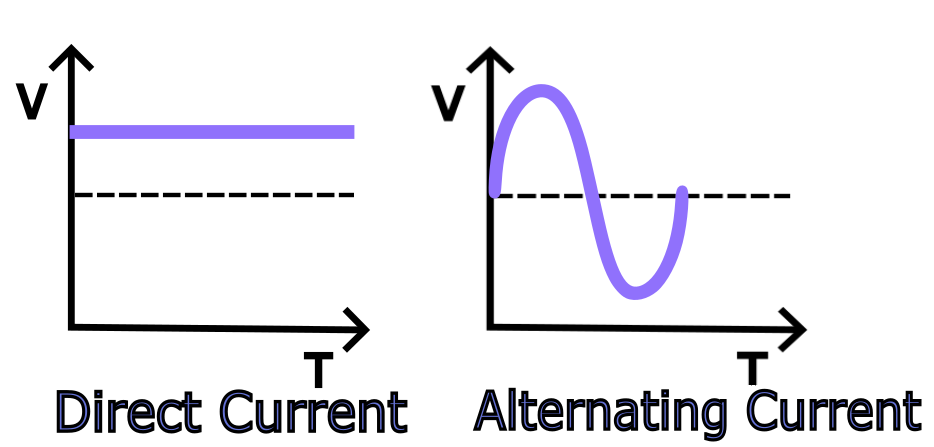
\includegraphics[width=1\textwidth]{AC_vs_DC.png}

In most countries, the RMS of the voltage between 110 and 240 V. (The
peak voltage is always $\sqrt{2}$ times the RMS value. In the US, for
example, people say ``Our outlets supply 120 V.'' They mean that the
RMS of the voltage difference between the wire and the earth is 120V.
The peak voltage is almost 170V.)

How much current can a human handle? Not much. You can barely feel 1
mA moving through your body, but at 16 mA, your muscles will clench
and you won't be able to relax them -- many people die from
electrocution because they grab a wire which pushes enough current
through their body to prevent them from letting go of the wire.  At 20
mA, a human's respiratory muscles become paralyzed.

The fuse breaker in a house will often allow 20 A to flow through the
circuit before it shuts off the power: Always, always, always shut off
the power before touching any of the wiring in your house.

While water is actually a mediocre conductor, it can still deliver enough current
to kill you. If you see a wire in a puddle, you should not touch the
puddle. Interestingly, because of the salt, sea water is more than
100 times better at conducting electricity than the water you drink.
% ADD: Sea of electrons makes a good conductor

% 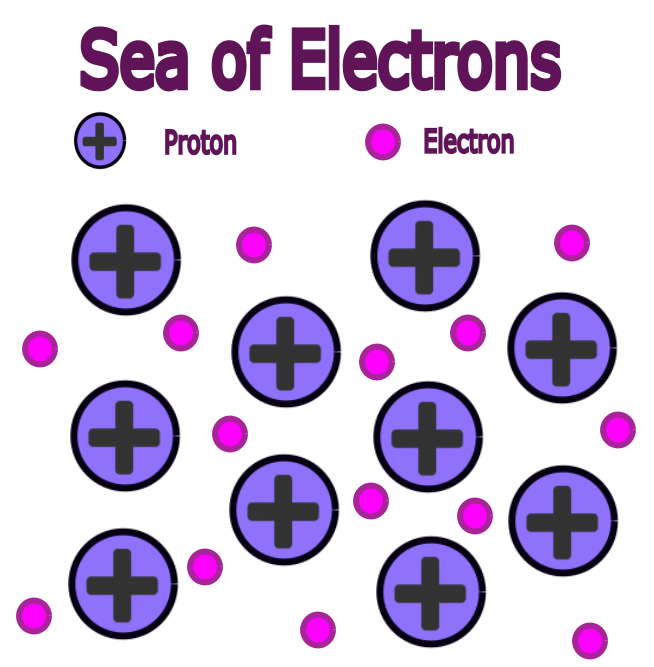
\includegraphics[width=0.8\textwidth]{Sea_Electrons.png}

If you hold a wire in each hand, how many Ohms of resistance will your
body have? Once it gets past your skin, you will look like a bag of
salt water to the electricity. After the skin, your body will have a
resistance of about 300$\Omega$. However, the skin is a pretty good
insulator. If you have dry, calloused hands, your skin may add a
100,000$\Omega$ to the resistance.

% KA: https://www.khanacademy.org/science/in-in-class10th-physics/in-in-electricity/in-in-electric-power-and-heating-effect-of-current/v/electric-power-energy


\graphicspath{{../../Chapters/dc_circuits/en_US}}
\chapter{DC Circuit Analysis}

In the most basic circuit, you have only a battery and a resistor:



\begin{circuitikz}
\draw (0,0) to[battery1,invert,l=$6V$] ++(0,3)
to ++(3,0)
to [R=$3\Omega$, /tikz/circuitikz/bipoles/length=1.0cm,i=2A] ++(0,-3) -- (0,0);
\end{circuitikz}

For this situation, you only need Ohm's Law: $V = I R$.  In this case, $6V = 3\Omega \times 2A$.
% ADD: Define Ohm's Law
\begin{Exercise}[title={Ohm's Law}, label=ohms_check]

  How many amps are going around the circuit?
  
  \vspace{1cm}

\begin{circuitikz}
\draw (0,0) to[battery1,invert,l=$24V$] ++(0,3)
to ++(3,0)
to [R=$6\Omega$, /tikz/circuitikz/bipoles/length=1.0cm,i={? A}] ++(0,-3) -- (0,0);
\end{circuitikz}

  
\end{Exercise}
\begin{Answer}[ref=ohms_check]

  $V = I R$ so $I = \frac{V}{R} = \frac{24V}{6\Omega} = 4A$.
  
\end{Answer}
% KA: https://youtu.be/F_vLWkkOETI

\section{Resistors in Series}

When you have two resistors wired together in a long line, we say they
are ``in series.''  If you have two resistors $R_1$ and $R_2$ wired in
series, the total resistance is $R_1 + R_2$.

In this diagram, for example, the total resistance is $5\Omega$.

\begin{circuitikz}
\draw (0,0) to[battery1,invert,l=$10V$] ++(0,5)
to ++(3,0)
to [R=$3\Omega$] ++(0,-2.5)
to [R=$2\Omega$] ++(0,-2.5) -- (0,0);
\end{circuitikz}

The current flowing through the circuit, then, is $10/5 = 2A$.

By Ohm's law, the voltage drop across the upper resistor is $I R = 2A \times 3\Omega = 6V$.

The voltage drop across the lower resistor is $I R = 2A \times 2\Omega = 4V$.

Notice that the battery pumps the voltage up to $10V$, then the two
resistors drop it by exactly $10V$. This is known as ``Kirchhoff's
Voltage Law'':
% KA: https://youtu.be/4rsswT_Rv1M

\begin{mdframed}[style=important, frametitle={Kirchhoff's Voltage Law}]\index{Kirchhoff's voltage law}
As you make a loop around a circuit, the sum of the voltage increase
must equal the sum of the voltage decrease.
\end{mdframed}

The negative end of the battery is connected to ``ground''\index{index} (it has zero voltage). We can then draw a diagram with the
voltages (That symbol in the lower right represents a connection to ground).

\begin{circuitikz}
\draw (0,0) to[battery1,invert,l=$6V$] ++(0,5) 
to [-*] ++(3,0) node[anchor=west] {10V}
to [R=$3\Omega$,-*] ++(0,-2.5) node[anchor=west] {4V}
to [R=$2\Omega$,-*] ++(0,-2.5) node[anchor=west]{0V} node[ground]{} --(0,0);
\end{circuitikz}


\begin{Exercise}[title={Resistors In Series}, label=series_resistor]

  What is the current going around the circuit?
  
  What is the voltage drop across each resistor?
  
  \vspace{1cm}
\begin{circuitikz}
\draw (0,0) to[battery1,invert,l=$16V$] ++(0,5) 
to [-*] ++(3,0) node[anchor=west] {16V}
to [R=$5\Omega$,-*] ++(0,-2.5) node[anchor=west] {?}
to [R=$3\Omega$,-*] ++(0,-2.5) node[anchor=west]{0V} node[ground]{} --(0,0);
\end{circuitikz}


\end{Exercise}
\begin{Answer}[ref=series_resistors]

  There is a total resistance of $8\Omega$, so your 16V will push 2A
  of current around the circuit.

  2A going through a $5\Omega$ resistor represents a 10V drop.

  2A going through a $3\Omega$ resitor represents a 6V drop.
  
\end{Answer}


\section{Resistors in Parallel}

Observe the following circuit. Note that the current can go two different paths.

\begin{circuitikz}
\draw (0,0) to[battery1,invert,l=$12V$] ++(0,3)
to ++(3,0)
to [R=$2\Omega$, /tikz/circuitikz/bipoles/length=1.0cm] ++(0,-3) -- (0,0);
\draw (3,3) -- (5,3)
to [R=$3\Omega$, /tikz/circuitikz/bipoles/length=1.0cm] ++(0,-3) -- (3,0);
\end{circuitikz}

There is 12 volts pushing current through both resistors. So 6A will
go through the 2$\Omega$ resistor and 4A will go through the 3$\Omega$
resistor. Note that even though there is a path of least resistance (2$\Omega$), the current is still devided evenly among both branches.

\begin{circuitikz}
\draw (0,0) to[battery1,invert,l=$12V$] ++(0,3)
to ++(3,0)
to [R=$2\Omega$, /tikz/circuitikz/bipoles/length=1.0cm,i=6A] ++(0,-3) -- (0,0);
\draw (3,3) -- (5,3)
to [R=$3\Omega$, /tikz/circuitikz/bipoles/length=1.0cm,i=4A] ++(0,-3) -- (3,0);
\end{circuitikz}

Thus, a total of 10 A will be going through the battery.

Imagine you are a battery. You can't see that you have two resistors.
What does it feel like to you? $\frac{V}{I} = R$, and $V= 12$ and $I =
10$. This means the effective resistance of the two resistors in parallel is
$\frac{12}{10}$ or $\frac{6}{5} \Omega$.

\begin{mdframed}[style=important, frametitle={Resistance in Parallel}]\index{resistance!in parallel}
If you have several resistances $R_1, R_2, \ldots, R_n$ wired in
parallel, their effective resistance $R_t$ is given by

$$\frac{1}{R_t} = \frac{1}{R_1} + \frac{1}{R_2} + \ldots + \frac{1}{R_n}$$

\end{mdframed}

In our example:

$$\frac{1}{R_t} = \frac{1}{2} + \frac{1}{3} = \frac{5}{6}$$

Thus, $R_t =  \frac{6}{5}\Omega$.

\begin{Exercise}[title={Resistors In Parallel}, label=parallel_resistors]

  What is the current going through the battery?
  What is the drop over the $4\Omega$ resistor?
  What is the current in each branch?

  \vspace{1cm}

  \begin{circuitikz}
\draw (0,0) to[battery1,invert,l=$12V$] ++(0,3)
to [R=$4\Omega$, /tikz/circuitikz/bipoles/length=1.0cm] ++(3,0) node [yshift=0.3cm] {? V}
to [R=$6\Omega$, /tikz/circuitikz/bipoles/length=1.0cm,i={? A}] ++(0,-3) node[ground]{} -- (0,0);
\draw (3,3) -- (5,3)
to [R=$3\Omega$, /tikz/circuitikz/bipoles/length=1.0cm,i={? A}] ++(0,-3) -- (3,0);
\end{circuitikz}

\end{Exercise}
\begin{Answer}[ref=parallel_resistors]
  The effective resistance of the $6\Omega$ and the $3\Omega$ is $2\Omega$ because 

  $$\frac{1}{R_T} = \frac{1}{6} + \frac{1}{3} == \frac{1}{2}$$

  This means the battery experiences a resistance of $4\Omega + 2\Omega =
  6\Omega$.  A $12V$ will push 2A through a resistance of $6\Omega$.

  The voltage drop across the $4\Omega$ resistor is $2A \times 4\Omega
  = 8V$. Thus there will be a 4V drop across the two resistors in
  parallel.  So 2/3 A will flow through the $6\Omega$ resistor. 4/3 A
  will flow through the $3\Omega$ resistor.

    \begin{circuitikz}
\draw (0,0) to[battery1,invert,l=$12V$] ++(0,3)
to [R=$4\Omega$, /tikz/circuitikz/bipoles/length=1.0cm] ++(3,0) node [yshift=0.3cm] {8 V}
to [R=$6\Omega$, /tikz/circuitikz/bipoles/length=1.0cm,i={2/3 A}] ++(0,-3) node[ground]{}-- (0,0);
\draw (3,3) -- (5,3)
to [R=$3\Omega$, /tikz/circuitikz/bipoles/length=1.0cm,i={4/3 A}] ++(0,-3) -- (3,0);
\end{circuitikz}
  
\end{Answer}


\graphicspath{{../../Chapters/charge/en_US}}
\chapter{Charge}

If you rub a balloon against your hair, then place it next to a wall, it will stick. This is because it stole some
electrons from your hair, and now the ballon has slightly more
electrons than protons. We say that it has gotten an \textit{electrical charge}. In this case, the balloon has a negative electrical
charge.

Objects with slightly more protons than electrons have a positive charge.

This charge is measured in coulombs. The charge of a single proton is
about $1.6 \times 10^{-19}$ coulombs.

An object with a negative charge and an object with a positive charge
will be attracted to each other. Two objects with the same charge will
be repelled by each other.
% ADD: Good place for culloms law
% KA: https://www.khanacademy.org/science/hs-physics/x215e29cb31244fa1:types-of-interactions/x215e29cb31244fa1:coulomb-s-law/v/coulombs-law

\begin{mdframed}[style=important, frametitle={Coulomb's Law}]\index{Coulomb's law}

  If two objects with charge $q_1$ and $q_2$ (in coulombs) are $r$ meters from each other, the force of attraction or repulsion is given by

  $$F = K\frac{\lvert q_1 q_2 \rvert}{r^2}$$

    where $F$ is in newtons and $K$ is Coulomb's constant: about $8.988 \times 10^9$.
  
\end{mdframed}


\begin{Exercise}[title={Coulomb's Law}, label=charged_balloons]

Two balloons are charged with an identical quantity and type of
charge: $-5 \times 10^{-9}$ coulombs. They are held apart at a
separation distance of 12 cm. Determine the magnitude of the
electrical force of repulsion between them. 
  
\end{Exercise}
\begin{Answer}[ref=charged_balloons]

  $$F = K\frac{\lvert q_1 q_2 \rvert}{r^2} = (8.988 \times 10^9) \frac{(-5 \times 10^{-9})(-5 \times 10^{-9})}{0.12^2} = \frac{224.7 \times 10^{-9}}{0.0144} = 15.6 \times 10^{-6}$$

  15.6 micronewtons.
  
\end{Answer}

At this point, you might ask ``If the wall has zero
charge, why is the balloon attracted to it?'' The answer: the
electrons in the wall move away from the balloon. The negative charge
on the balloon pushes electrons into the wall, so the surface of the
wall gets a mild positive charge. The surface is close to the balloon,
so the attraction is stronger than the repulsion.

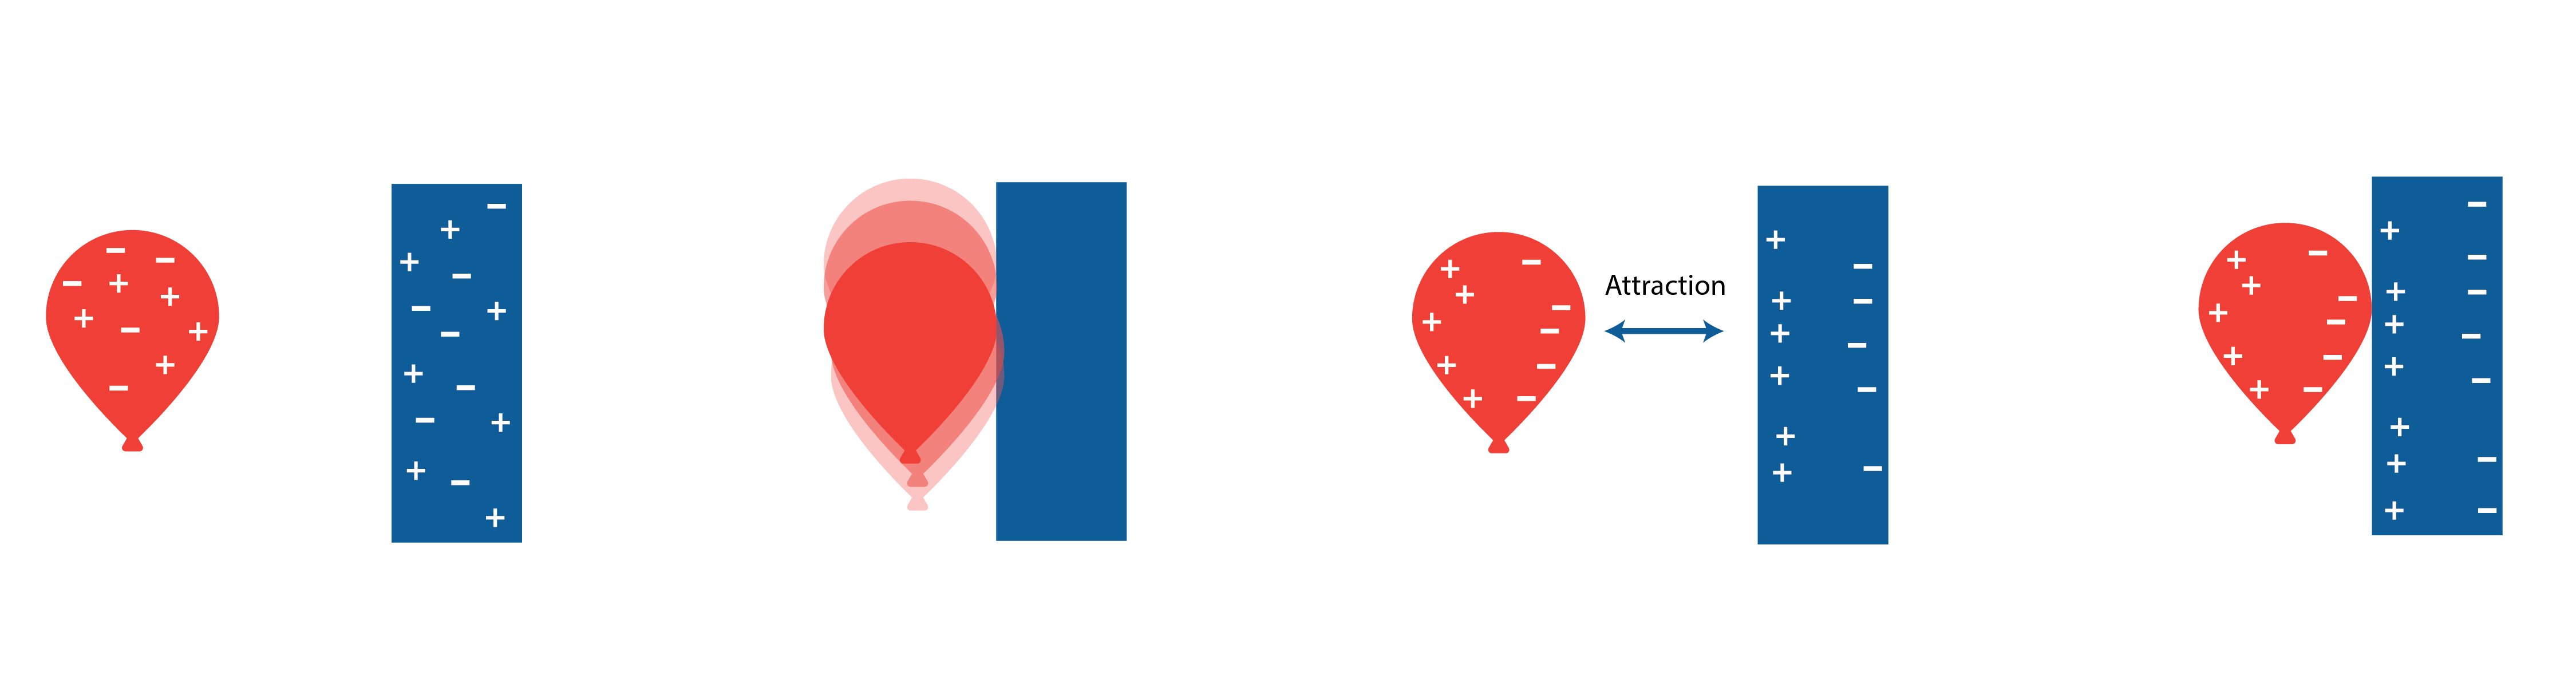
\includegraphics[width=1\textwidth]{balloon2.png}

\section{Lightning}

A cloud is a cluster of water droplets and ice particles. These
droplets and ice particles are always moving up and down through the
cloud. In this process, electrons get stripped off and end up on the
water droplets at the bottom of the cloud (water droplets collect at the bottom because they are denser). The air between the
droplets is a pretty good insulator, which means the electrons are reluctant
to jump anywhere. However, eventually, the charge gets so strong that
even the insulating properties of the air is not enough to prevent
the jump, causing lightning.
% ADD: Add water density explanation. ice less dense than liquid water due to crystaline structure.

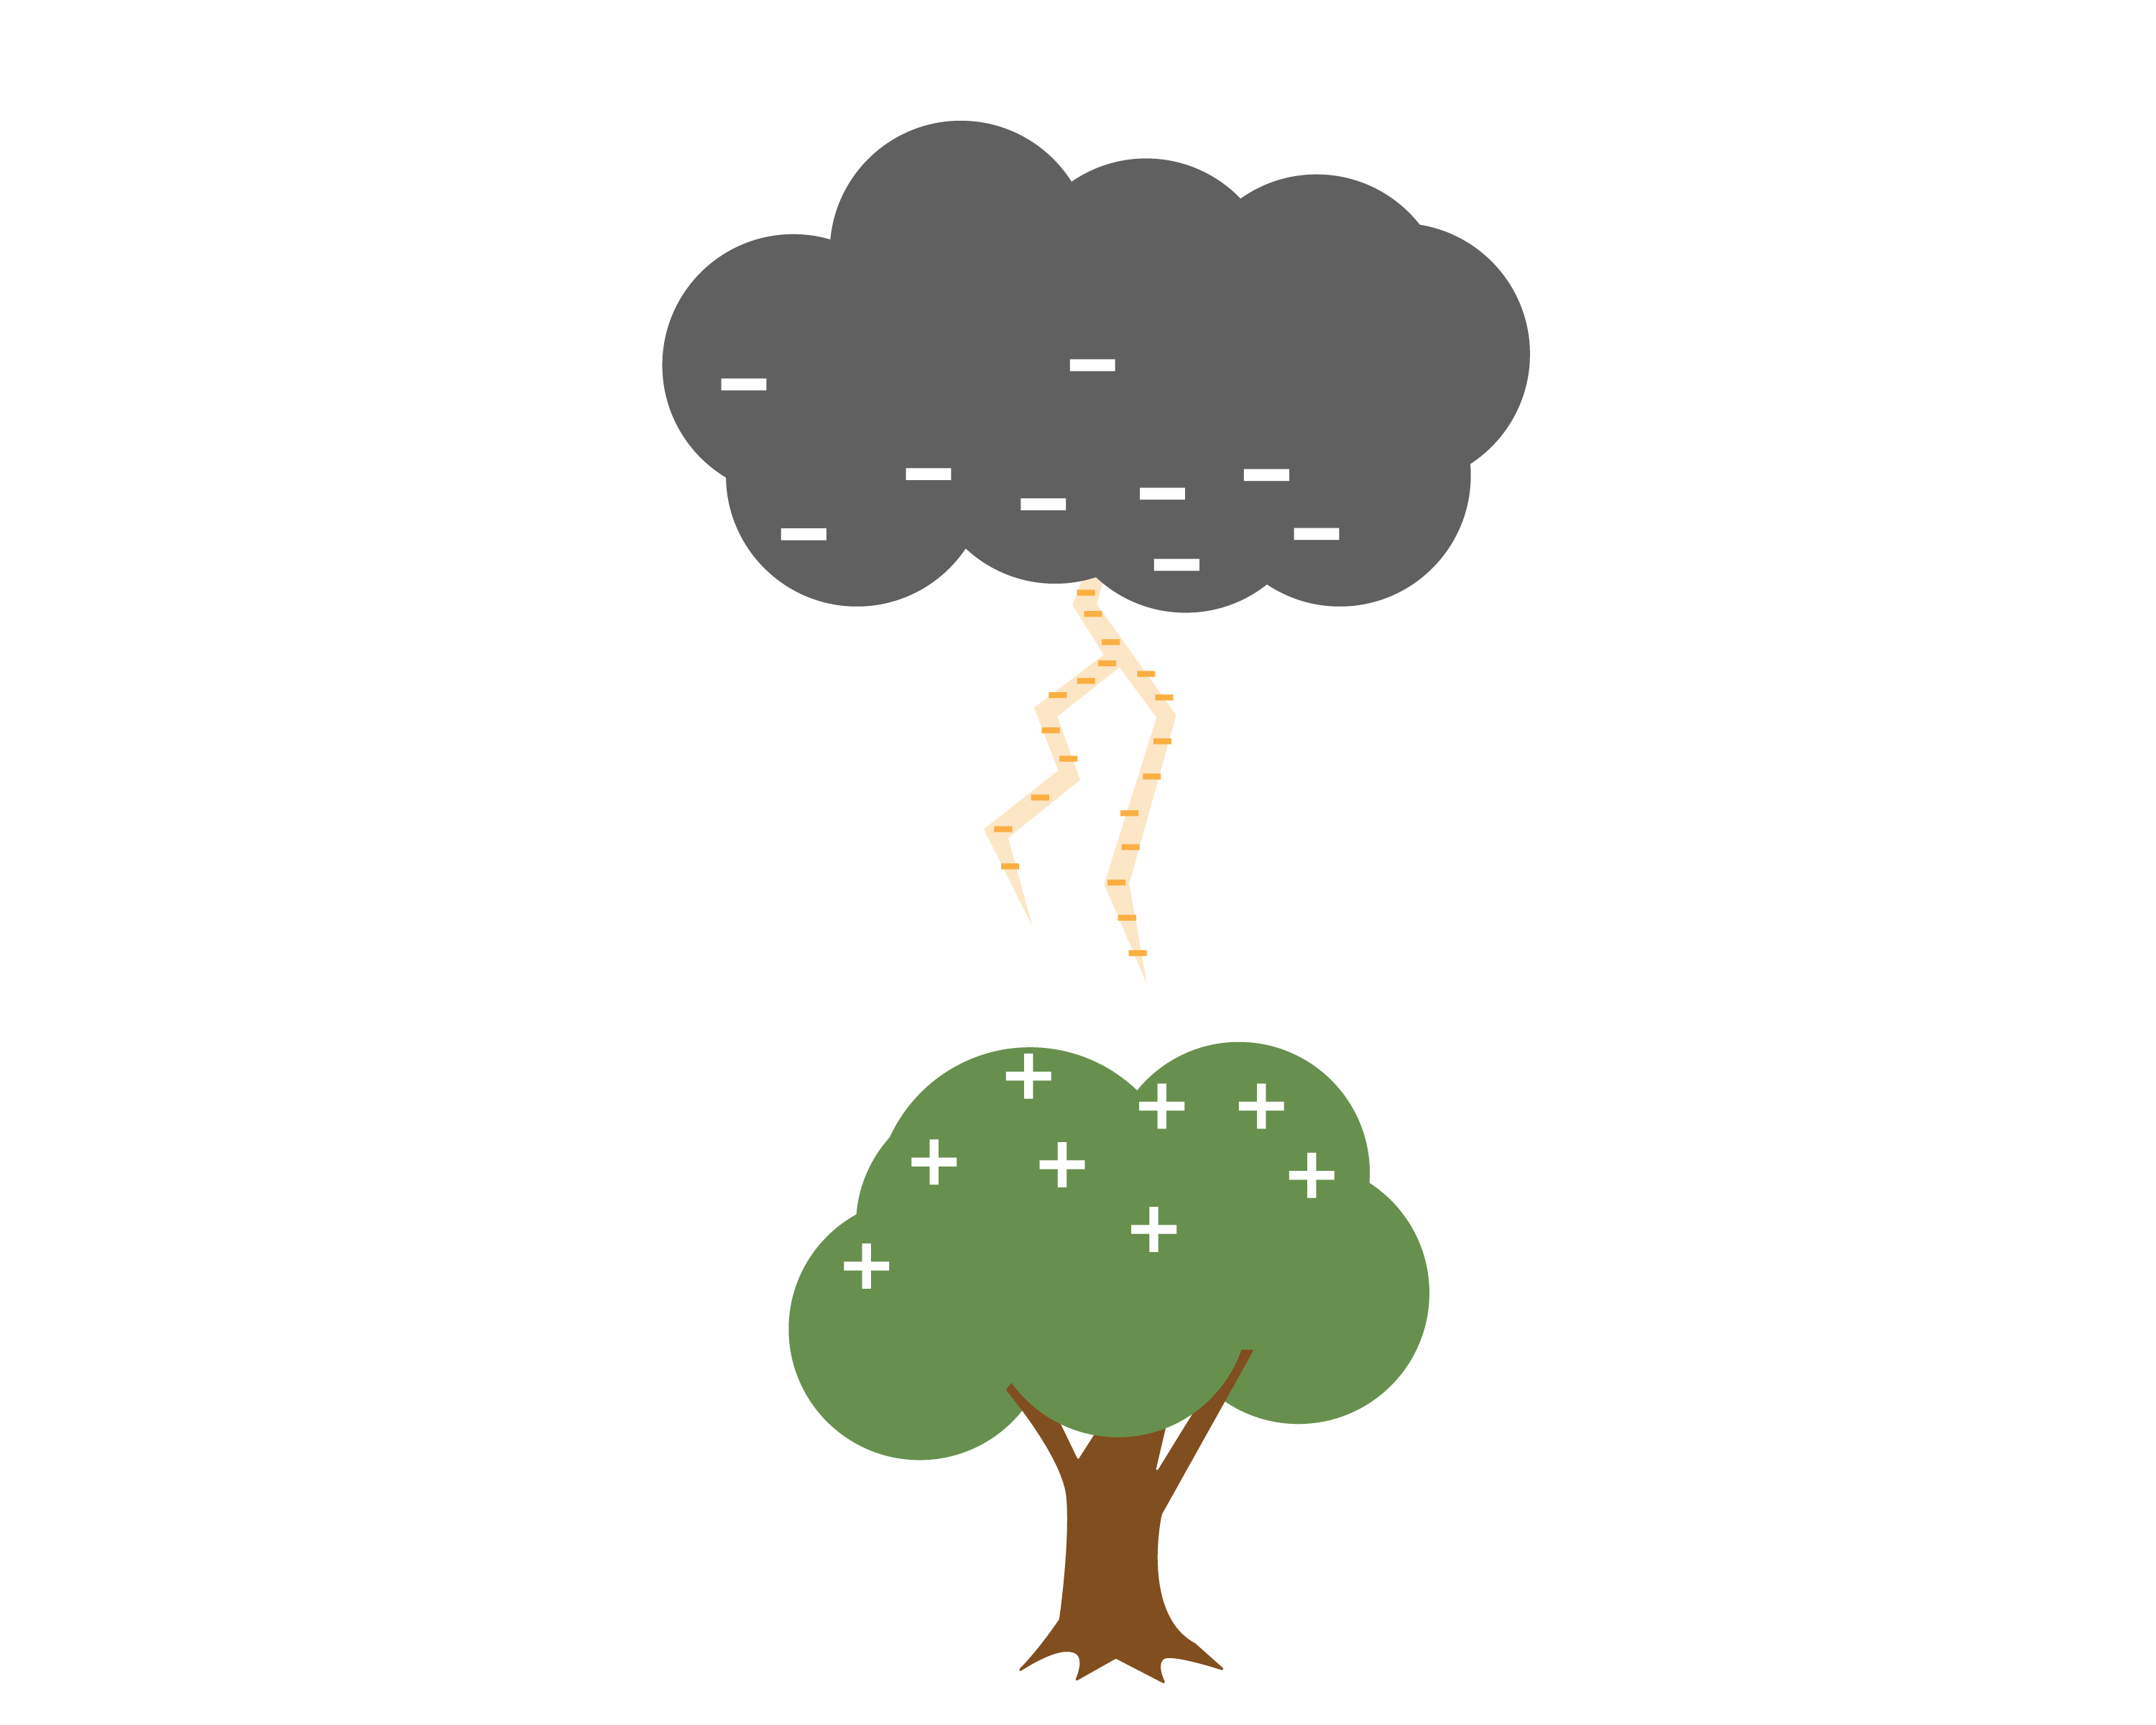
\includegraphics[width=1\textwidth]{lightning.png}

A great deal of lightning moves within a cloud or between clouds. However, sometimes it jumps to the earth. These bolts of lightning vary in the amount of
electrons they carry, but the average is about 15 coulombs.

Thunder occurs because the electrons heat the air they pass through, 
causing the air to expand suddenly. Tthe resulting shockwave is the sound we know as thunder.
% ADD: Relate speed of light and sound 
\section{But...}

This idea that opposite charges attract creates some heavy questions
that you do not yet have the tools to work with. So to these questions, the answer is
basically ``Don't ask that yet!''

However, you probably have these questions, so we will point you in
the direction of the answers.

The first is ``In any atom bigger than hydrogen, there are multiple
protons in the nucleus. Why don't the protons push each other out of
the nucleus?''

We aren't ready to talk about it, but there is a force called \textit{the
 nuclear force}, which pulls the protons and neutrons in the nucleus
of the atom toward each other. At very, very small distances, it is
strong enough to overpower the repulsive force due to the protons'
charges.
% ADD: Effective nuclear charge

Another question is ``Why do the electrons whiz around in a cloud so
far from the nucleus of the atom? Negatively charged electrons should
cling to the protons in the center, right?''

We aren't ready to talk about this either, but quantum mechanics tells us that
electrons like to live in a certain specific energy level. Hugging
protons isn't one of those levels.


\graphicspath{{../../Chapters/fertilizer/en_US}}
\chapter{Fertilizer}

FIXME 
First, Allison has learned she does not need a colon after FM

\textit{Here are some thoughts on expanding the introduction to the Fertilizer Chapter. This might be a good moment to discuss the multidisciplinary nature of Kontinua. 
In a regular science class I'm guessing you wouldn't get electricity and Fertilizer in the same textbook. Why is there a chapter on Fertilizer here? Are you introducing us to the major ways science has given us more power and allowed population to grow? Can we discuss your thoughts on why problem solvers need a basic understanding of Fertilizer and I'll write up a new introduction to this chapter based on the discussion?}


\textit{What do you think about adding a conclusion that talks about the connection between fertilizer (nitrogen), dynamite and the origin of the Nobel peace prize? I know you don't want too much history and philosophy but this seems like a great moment to add a little narrative spice}.

\textit{Can we work POTATOES into this chapter!?!}

Chapter text starts here: 

One of the biggest problems humans face is: how can we get enough food to feed everyone?
In 1950, there were 2.5 billion people on the planet, and about 65\%
were malnourished. In 2019, there were 7.7 billion people on the
planet, and only 15\% are malnourished. How did crop yields increase
so much? There were several factors: better crop varieties,
reliable irrigation, increased mechanization, and affordable fertilizers.\index{fertilizer}

When a plant grows, it takes molecules out of the soil and uses them
to build proteins. It primarily needs the elements nitrogen ($N$),
phosphorus ($P$), and potassium ($K$).\index{nitrogen} \index{phosphorus} \index{potassium}

When you buy a bag of fertilizer at the store, it typically has
three numbers on the front. For example, you might buy a bag of
``24-22-4''.  This means that 24\% of the mass of the bag is nitrogen,
22\% is phosphorus, and 4\% is potassium.

Potassium comes as potassium carbonate ($K_2CO_3$), potassium chloride
($KCl$), potassium sulfate ($K_2 SO_4$), and potassium nitrate
($KNO_3$). Any blend of these chemicals is known as ``potash''. Potash
is dug up out of mines. \index{potash}

Phosphorus is also mined, but is refined into phosphoric acid
($H_3PO_4$) before it is put into fertilizer.

Nitrogen is an especially interesting case for 2 reasons:
\begin{itemize}
\item Worldwide, farmers apply more nitrogen to their soil than potassium or phosphorous combined.
\item 78\% of the air we breathe is nitrogen in the form of $N_2$, but
  neither plants nor animals can utilize nitrogen in that form.
\end{itemize}

\section{The Nitrogen Cycle}

Converting the $N_2$ in the air into a form that a plant can use
is known as \newterm{nitrogen fixation}. For billions of years, there
were only two ways that nitrogen fixation occurred on earth:
\begin{itemize}
\item The energy from lightning causes $N_2$ and $H_2O$ to reconfigure as ammonia ($NH_3$) and nitrate ($NO_3$). This accounts for about 10\% of all naturally occurring nitrogen fixation.
\item Cyanobacteria are responsible for the rest. They convert $N_2$ into ammonia.
\end{itemize}\index{nitrogen cycle} \index{nitrogen fixation}

Let's say that you are eating soybeans. There is a cyanobacteria
called \newterm{rhizobia} that has a symbiotic relationship with
soybean plants. Rhizobia fixes nitrogen for the soybean plant. The
soybean plant performs photosynthesis, then gives sugars to the
rhizobia.

The proteins in the soybeans contain nitrogen from the rhizobia. When
you eat them, you use some of the nitrogen to build new proteins. You
probably don't use all the nitrogen, so your cells release ammonia into your blood.

Ammonia likes to react with things, so your liver combines the ammonia
with carbon dioxide to make urea ($CO(NH_2)_2$). Your kidneys take
the urea out of your blood and mix it with a bunch of water and salts
in your bladder.  When you urinate, the urea leaves your body.\index{urea}

If you urinate on the ground, the nearby plants can take the nitrogen out of
the urea.\index{urine}

When you die, the nitrogen in your proteins will return to the soil as
ammonia and nitrate.

For centuries, farms got their nitrogen from urine, feces, and rotting
organic material. There were two challenges with this:
\begin{itemize}
\item Human pathogens had to be kept away from human food.
\item There was simply not enough to support 7.7 billion people.
\end{itemize}

This meant we had to figure out how to do nitrogen fixation at an industrial
level.

\section{The Haber-Bosch Process}

During World War I, two German scientists, Fritz Haber and Carl Bosch,
figured out how to make ammonia from $N_2$ and $H_2$ using high
temperatures and pressures. This is how nearly all nitrogen fertilizer
is created today.\index{Haber-Bosch process}

Where do we get the $H_2$? From methane ($CH_4$) in natural gas. Today, 3-5\%
of the world's natural gas production is consumed in the Haber-Bosch
process.

The ammonia is converted into ammonium nitrate ($NH_4NO_3$) or urea
before it is shipped to farms.

\section{Other nutrients}

Healthy plants require several other elements that are sometimes
applied as fertilizer: calcium, magnesium, and sulfur.

Finally, tiny amounts of copper, iron, manganese, molybdenum, zinc, and
boron are sometimes needed.

%FIXME add photosynthesis process here?
\graphicspath{{../../Chapters/concrete/en_US}}
\chapter{Concrete}

To make concrete, you mix cement with water and an aggregate (sand or
rock).  The cement is usually only about 10 to 15 percent of the
mixture. The cement reacts with the water, and the resulting solid
binds the aggregate together. In 2019, the world consumed 4.5 billion
tons of cement.\index{concrete} \index{cement}

Concrete is hard and durable. The mortar between the pyramids at Giza
is concrete --- it is now 5000 years old. Today, we use concrete to
build many structures including buildings, bridges, airport runways,
and dams. Grout and mortar are related materials but different in that 
they are used as bonding or filler materials within construction.


There are many kinds of cement, but the most common is Portland
cement. It is made by heating limestone (calcium carbonate) with clay
(for silicon) in a kiln. Two things come out of the kiln: Carbon
dioxide and a hard substance called ``clinker''.  The clinker is
ground up with some gypsum before it is sent to market. 

The carbon dioxide is released into the atmosphere, making it an exothermic reaction. Cement manufacturing
is responsible for about 8\% of the world's $CO_2$ emissions; it is a
major contributor to climate change.

Especially hard concrete, like that used in a nuclear power plant, can
support 3,000 kg per centimeter without being crushed. However, if
you pull on two ends of a piece of concrete, it comes apart relatively
easily. We say that concrete can handle a lot of \newterm{compressive
  stress}, but not much \newterm{tensile} stress.

\section{Steel reinforced concrete}

Many places where we use concrete (like in a bridge), we need both
compressive and tensile stress. Often, the top of a beam is undergoing
compression and the bottom of the beam is undergoing tension.

FIXME Picture here
% https://letstalkscience.ca/educational-resources/backgrounders/why-a-triangle-a-strong-shape

Steel has tremendous tensile strength, but not as much compressive
strength as concrete. To get both tensile \emph{and} compressive
strength, we often bury steel bars or cables inside the concrete.
This is known as \newterm{steel-reinforced concrete}. The concrete
generally does a very good job protecting the steel, which keeps it
from rusting.\index{steel reinforced concrete}

You may have heard of \newterm{rebar} before. That is just short for
``reinforcing bar''.  Typically, rebar has bumps and ridges that keep
the bar and the concrete from moving independently.\index{rebar}

\section{Recycling concrete}

Many concrete structures only last about 100 years. When they are
demolished, the concrete can be reused as aggregate in other projects.
Often, the concrete bits are mixed with cement and made into concrete once more.

If the concrete to be reused is reinforced with steel, the steel has
to be removed and recycled separately.  The concrete is then crushed
into small pieces.

\graphicspath{{../../Chapters/metals/en_US}}
\chapter{Metals}

Elements that transmit electricity well, even at low temperatures, are
called \newterm{metals}. Many metals are likely familiar to you, such as
aluminum, iron, copper, tin, gold, silver, and platinum. Aluminum and
iron are particularly common; together they make up about 14\% of the
earth's crust.

An \newterm{alloy} is a mixture of elements that includes at least one
metal. Brass, for example, is an alloy of copper and zinc.  Bronze is
an alloy of copper and tin.



\section{Steel}

One of the most common alloys is steel, which is an alloy of iron and carbon.
In pure iron, the molecules slip past each other easily, so pure iron
is relatively soft and easily deformed. The carbon in steel prevents
that slipping, which is why steel is much, much harder than iron.

How much carbon does steel have? If you have less than 0.002\% by weight, you end up
with something very much like pure iron.  As you increase the carbon,
it gets harder and harder. Once it gets above about 2\%, the result
is very brittle.

If you add about 11\% chromium to steel, you get \newterm{stainless
  steel}, which resists rusting.

\begin{Exercise}[title={Tensile Strength}, label=tensile-mpa]

The tensile strength of steel is usually between 400 MPa and 1200
MPa. A Mega Pascal (MPa) is the strength necessary to hold 1,000,000 newtons of
force with a cable that has a 1 square meter cross section. Or,
equivalently, to hold 1 newton of force with a cable that has a 1
square millimeter cross section. 

If you have are buying a round cable that has a tensile strength of
700 Mpa and must hold a 100 kg man aloft, what is the diameter of the
smallest cable you can use?
  
\end{Exercise}
\begin{Answer}[ref=tensile-mpa]
On earth, holding a 100 kg man aloft requires 980 Newtons of force.

$980/700 = 1.4$, so you need a cable with a cross-section area of 1.4
square millimeters.

$$\pi r^2 = 1.4$$

$r = \sqrt{1.4/\pi} \approx .67$ millimeters. This means the cable would
have to have a diameter of at least 1.34 millimeters.

\end{Answer}

Here are some approximate tensile strengths of other materials:

\begin{tabular}{c|c}
  Material & Tensile strength (MPa) \\
  \hline
  Iron & 3 \\
  Concrete & 4 \\
  Rubber & 16 \\
  Glass & 33 \\
  Wood & 40 \\
  Nylon & 100 \\
  Human hair & 200 \\
  Aluminum  & 300 \\
  Steel & 700 \\
  Spider webs & 1000 \\
  Carbon fiber & 4000
\end{tabular}

\section{What metal for what task?}

Copper is often used for electrical wires in your house and
appliances. This is because it is very efficient at moving electricity (very
little power is lost as heat). It is also very good a transmitting
heat, so you will often see copper pots and pans.

Aluminum is less dense than copper, and is still a relatively good
conductor of electricity. This combination of lighter weight and conductivity is why the overhead wires in a power system
are often made of aluminum.

Aluminum is not as strong as steel, but considerably lighter. It is
often used structurally where weight is a concern, such as in skyscrapers, cars,
airplanes, and ships.

Titanium is about as strong as steel, but it weights about half as
much. Titanium is very difficult to work with, so it is used in places
where weight and strength are very important and cost is not, such as in
airplanes and bicycles.
FIXME: We mention airplanes in both examples. Maybe we should clarify the role each one plays?

(Carbon fiber, which is light, strong, and very easy to work with, is
replacing aluminum and titanium in many applications. 20 years ago,
many expensive bicycles were made of titanium. These days the vast
majority are made with carbon fiber.)

Zinc and tin are very resistant to corrosion, so they are often used
as a coating to prevent steel from rusting. They are also used in many
alloys for the same reason.  In the United States, the penny is 97.5\%
zinc and only 2.5\% copper.


\graphicspath{{../../Chapters/angles/en_US}}
\chapter{Angles}

In the following recommend videos, the narrator talks about
lines, line segments, and rays. When mathematicians talk about
\emph{lines}\index{lines}, they mean a straight line that goes forever in two 
directions. And if you pick any two points on that line; the space between 
them is a \emph{line segment}\index{line segment}. If you take any line, pick 
a point on that line and discard all the points on one side of the point, that 
is a \emph{ray}\index{ray}. All three have no width.

\begin{center}
\begin{tikzpicture}[scale=1.5]
  \coordinate (a) at (-0.3, -0.6);
  \coordinate (d) at (1.3, 2.6);
  \draw [<->](a)--node [right]{"Line"}(d);
\end{tikzpicture}
\hspace{10mm}
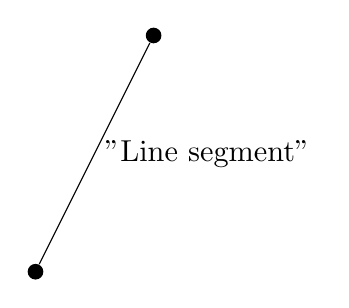
\begin{tikzpicture}[scale=1.5]
  \coordinate [circle, fill, inner sep=2pt] (b) at (0,0) ;
  \coordinate [circle, fill, inner sep=2pt] (c) at (1, 2) ;
  \draw (b)--node [right]{"Line segment"}(c);
\end{tikzpicture}
\hspace{6mm}
\begin{tikzpicture}[scale=1.5]
  \coordinate [circle, fill, inner sep=2pt] (b) at (0,0) ;
  \coordinate (d) at (1.3, 2.6);
  \coordinate (lab) at (0.8, 1.0);
  \draw [->](b)--node[right] {"Ray"} (d)  ;
\end{tikzpicture}
\end{center}



Watch the following videos from Khan Academy:
\begin{itemize}
\item Introduction to angles: \url{https://youtu.be/H-de6Tkxej8}
\item Measuring angles in degrees: \url{https://youtu.be/92aLiyeQj0w} 
\end{itemize}

When two lines cross, they form four angles:

\begin{center}
\begin{tikzpicture}[scale=3]
  \coordinate (a) at (0, 1.5);
  \coordinate (b) at (1.6, 2);
  \coordinate (c) at (1.6, 1.5);
  \coordinate (d) at (0, 1);
  \coordinate [circle, fill, inner sep=1pt](e) at (0.8, 1.5) ;
  \draw [->](e)--(a) node[left] {$A$}  ;
  \draw [->](e)--(b) node[right] {$B$}  ;
  \draw [->](e)--(c) node[right] {$C$}  ;
  \draw [->](e)node[above]{$E$}--(d) node[left] {D} ;
  \pic [draw, <->, "$\scriptstyle  \angle AEB$ ", angle radius = 0.8cm, 
  angle eccentricity=1.3] {angle = b--e--a};
  \pic [draw, <->, "$\scriptstyle  \angle BEC$ ", angle radius = 1.1cm, 
  angle eccentricity = 1.5] {angle = c--e--b};
  \pic [draw, <->, "$\scriptstyle  \angle CED$ ", angle radius = 0.8cm, 
  angle eccentricity=1.3] {angle = d--e--c};
  \pic [draw, <->, "$\scriptstyle  \angle DEA$ ", angle radius = 1.1cm, 
  angle eccentricity=1.5] {angle = a--e--d};
\end{tikzpicture}
\end{center}


What do we know about those angles?
\begin{itemize}
\item The sum of any two adjacent angles add to be $180^\circ$.  So, for 
example, $m \angle AEB + m \angle BEC = 180^\circ$. We use the phrase ``add to 
be $180^{\circ}$'' so often that we have a special word for it: 
\emph{supplementary}.\index{supplementary angles}
\item The sum of all four angles is $360^\circ$.
\item Angles opposite each other are equal. So, for example, $m \angle AEB = m 
\angle CED$.
\end{itemize}

In a diagram, to indicate that two angles are equal we often put hash marks in 
the angle:

\begin{center}
\begin{tikzpicture}[scale=3]
  \coordinate (a) at (0, 1.5);
  \coordinate (b) at (1.6, 2);
  \coordinate (c) at (1.6, 1.5);
  \coordinate (d) at (0, 1);
  \coordinate [circle, fill, inner sep=1pt](e) at (0.8, 1.5) ;
  \draw [->](e)--(a) node[left] {$A$}  ;
  \draw [->](e)--(b) node[right] {$B$}  ;
  \draw [->](e)--(c) node[right] {$C$}  ;
  \draw [->](e)node[above]{$E$}--(d) node[left] {D} ;
  \tkzMarkAngle[size = 0.2cm,mark = |](b,e,a)
  \tkzMarkAngle[size = 0.3cm,mark = ||](c,e,b)
  \tkzMarkAngle[size = 0.2cm,mark = |](d,e,c)
  \tkzMarkAngle[size = 0.3cm,mark = ||](a,e,d)
\end{tikzpicture}
\end{center}


Here the two angles with a single hash mark are equal and the two angles with 
double hash marks are equal.

When two lines are perpendicular, the angle between them is $90^\circ$ and we 
say they meet at a \emph{right angle}. When drawing diagrams, we indicate right
angles with an elbow:

\begin{center}
\begin{tikzpicture}[scale=1.5]
  \coordinate (a) at (0, 1.5);
  \coordinate (b) at (0, 0);
  \coordinate (c) at (1.5, 0);
  \draw [->](b)--(a)  ;
  \draw [->](b)--(c)  ;
  \pic [draw,thick,angle eccentricity=.5]{right angle = a--b--c};
\end{tikzpicture}
\end{center}

 
When an angle is less than $90^\circ$, it is said to be
\emph{acute}. When an angle is more than $90^\circ$, it is said to be
\emph{obtuse}.
% Add: Complementary Angles

\begin{center}
\begin{tikzpicture}[scale=3]
  \coordinate (a) at (0.4, 0.6);
  \coordinate (b) at (0, 0);
  \coordinate (c) at (0.9, 0);
  \draw [->](b)--(a)  ;
  \draw [->](b)--(c)  ;
  \pic [draw, <->, "acute", angle radius = 1cm, angle eccentricity=1.5] {
  angle = c--b--a};
  \end{tikzpicture}
\hspace{2cm}
\begin{tikzpicture}[scale=3]
  \coordinate (a) at (1, 0.6);
  \coordinate (b) at (0.5, 0);
  \coordinate (c) at (0, 0);
  \draw [->](b)--(a)  ;
  \draw [->](b)--(c)  ;
  \pic [draw, <->, "obtuse", angle radius = 0.6cm, angle eccentricity=1.5] {
  angle = a--b--c};
\end{tikzpicture}
\end{center}


If two lines are parallel, line segments that intersect both lines, form the 
same angles with each line:

\begin{center}
\begin{tikzpicture}[scale=3]
  \coordinate (a) at (0, 1);
  \coordinate [circle, fill, inner sep=1pt](b) at (1.5, 1.5);
  \coordinate (c) at (1.5, 1);
  \coordinate (d) at (0.5, 0.5);
  \coordinate (e) at (1, 1);
  \coordinate (f) at (0, 0.5);
  \coordinate (g) at (1.5, 0.5);
  \coordinate [circle, fill, inner sep=1pt](h) at (0, 0);
  \draw [->](e)--(a);
  \draw [-](e)--(b);
  \draw [->](e)--(c);
  \draw [-](e)--(d);
   \draw [->](d)--(f);
  \draw [->](d)--(g);
  \draw [-](d)--(h);
  \tkzMarkAngle[size = 0.15cm,mark = |](b,e,a)
  \tkzMarkAngle[size = 0.2cm,mark = ||](c,e,b)
  \tkzMarkAngle[size = 0.15cm,mark = |](d,e,c)
  \tkzMarkAngle[size = 0.2cm,mark = ||](a,e,d)
  
   \tkzMarkAngle[size = 0.15cm,mark = |](e,d,f)
  \tkzMarkAngle[size = 0.2cm,mark = ||](g,d,e)
  \tkzMarkAngle[size = 0.15cm,mark = |](h,d,g)
  \tkzMarkAngle[size = 0.2cm,mark = ||](f,d,h)
\end{tikzpicture}
\end{center}


\section{Radians}
As you've seen above, angles can be measured in degrees. Just like you can 
measure length in more than one unit (inches, meters, etc.), there is more 
than one unit to measure angles in. Angles can also be measured in \textit{
radians}\index{radians}. Radians are unitless (that is, you don't have to put 
a letter after the number) and there are $\pi$ radians across a straight line. 
This means $180^\circ$ is the same as $\pi$ radians. 

\textbf{Example}: An angle is measured to be $\frac{\pi}{2}$ radians. What is 
the angle in degrees?

\textbf{Solution}: Since we know that $\pi$ radians is the same as $180^\circ$,
we can set up the unit conversion:
$$\frac{\pi}{2} \cdot \frac{180^\circ}{\pi} = 90^o$$

Therefore, a $\frac{\pi}{2}$ angle is $90^\circ$. 

\begin{Exercise}[label = radians]
Convert the following angles from degrees to radians or from radians to degrees. 
\begin{enumerate}
\item $360^\circ$
\item $\frac{\pi}{3}$
\item $225^\circ$
\item $\frac{3\pi}{4}$
\item $30^\circ$
\item $45^\circ$
\end{enumerate}
\end{Exercise}

\begin{Answer}[ref = radians]
\begin{enumerate}
\item $2\pi$
\item $60^\circ$
\item $\frac{5\pi}{4}$
\item $135^\circ$
\item $\frac{\pi}{6}$
\item $\frac{\pi}{4}$
\end{enumerate}
\end{Answer}




\graphicspath{{../../Chapters/triangles_circles/en_US}}
\chapter{Introduction to Triangles}

Connecting any three points with three line segments will get you a
triangle. Here is the triangle $ABC$ which was created by connecting three points $A$, $B$, and $C$:\index{triangle}

\begin{tikzpicture}[scale=1.5]
  \coordinate [circle, fill, inner sep=2pt] (a) at (0,0) ;
  \coordinate [circle, fill, inner sep=2pt] (b) at (1, 2) ;
  \coordinate [circle, fill, inner sep=2pt] (c) at (3,0) ;
  \draw (a)--(b) node [outer sep=3pt, above]{$B$};
  \draw (b)--(c) node[outer sep=3pt, right]{$C$};
  \draw (c)--(a) node[outer sep=3pt, left]{$A$};
\end{tikzpicture}

\section{Equilateral and Isosceles Triangles}
% Add scalene Triaganle
We talk a lot about the length of the sides of triangles. If all three sides of the triangle are the same length, we say it is an \emph{equilateral triangle}:\index{equilateral triangle}

\begin{tikzpicture}[scale=1.5]
  \coordinate [circle, fill, inner sep=2pt] (a) at (0,0) ;
  \coordinate [circle, fill, inner sep=2pt] (b) at (1.5, 2.6) ;
  \coordinate [circle, fill, inner sep=2pt] (c) at (3,0) ;
  \draw (a)--(b) node [outer sep=3pt, above]{$B$};
  \draw (b)--(c) node[outer sep=3pt, right]{$C$};
  \draw (c)--(a) node[outer sep=3pt, left]{$A$};
  \tkzMarkSegment[pos=.5,mark=||](a,b)
  \tkzMarkSegment[pos=.5,mark=||](b,c)
  \tkzMarkSegment[pos=.5,mark=||](c,a)
\end{tikzpicture}

If only two sides of the triangle are the same length, we say it is an \emph{isosceles triangle}:\index{isoscelese triangle}

\begin{tikzpicture}[scale=1.3]
  \coordinate [circle, fill, inner sep=2pt] (a) at (0,0) ;
  \coordinate [circle, fill, inner sep=2pt] (b) at (1.5, 4) ;
  \coordinate [circle, fill, inner sep=2pt] (c) at (3,0) ;
  \draw (a)--(b) node [outer sep=3pt, above]{$B$};
  \draw (b)--(c) node[outer sep=3pt, right]{$C$};
  \draw (c)--(a) node[outer sep=3pt, left]{$A$};
  \tkzMarkSegment[pos=.5,mark=||](a,b)
  \tkzMarkSegment[pos=.5,mark=||](c,b)
\end{tikzpicture}

The shortest distance between two points is always the straight line
between them. Thus, you can be certain that the length of one side
will \emph{always} be less than the sum of the lengths of the
remaining two sides. This is known as the \emph{triangle inequality}.\index{triangle inequality}

For example, in this diagram $c$ must be less than $a + b$.

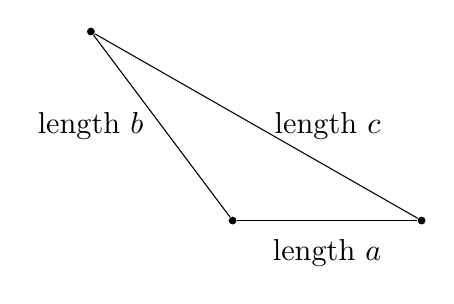
\begin{tikzpicture}[scale=1.2]
  \coordinate [circle, fill, inner sep=1pt] (a) at (1.5,0) ;
  \coordinate [circle, fill, inner sep=1pt] (b) at (0,2) ;
  \coordinate [circle, fill, inner sep=1pt] (c) at (3.5,0) ;
  \draw (a)--node[outer sep=3pt, left]{length $b$}(b) ;
  \draw (b)--node[outer sep=3pt, right]{length $c$}(c) ;
  \draw (c)--node[outer sep=3pt, below]{length $a$}(a) ;
\end{tikzpicture}

\section{Interior Angles of a Triangle}

We also talk a lot about the interior angles of a triangle:

\begin{tikzpicture}[scale=2]
  \coordinate [circle, fill, inner sep=2pt] (a) at (0,0) ;
  \coordinate [circle, fill, inner sep=2pt] (b) at (1, 2) ;
  \coordinate [circle, fill, inner sep=2pt] (c) at (3,0) ;
  \draw (a)--(b) node [outer sep=3pt, above]{$B$};
  \draw (b)--(c) node[outer sep=3pt, right]{$C$};
  \draw (c)--(a) node[outer sep=3pt, left]{$A$};
  \pic [draw, <->, "$a$", angle eccentricity=1.5] {angle = c--a--b};
  \pic [draw, <->, "$b$", angle eccentricity=1.5] {angle = a--b--c};
  \pic [draw, <->, "$c$", angle eccentricity=1.5] {angle = b--c--a};
\end{tikzpicture}

A triangle where one of the interior angles is a right angle is said to be a \emph{right triangle}:\index{right triangle}

\begin{tikzpicture}[scale=1.2]
  \coordinate [circle, fill, inner sep=2pt] (a) at (0,0) ;
  \coordinate [circle, fill, inner sep=2pt] (b) at (0,4) ;
  \coordinate [circle, fill, inner sep=2pt] (c) at (3,0) ;
  \draw (a)--(b) node [outer sep=3pt, above]{$B$};
  \draw (b)--(c) node[outer sep=3pt, right]{$C$};
  \draw (c)--(a) node[outer sep=3pt, left]{$A$};
  \pic [draw,angle eccentricity=1.5] {right angle = c--a--b};
\end{tikzpicture}

If a triangle has an obtuse interior angle, it is said to be an \emph{obtuse triangle}:\index{obtuse triange}

\begin{tikzpicture}[scale=1.2]
  \coordinate [circle, fill, inner sep=2pt] (a) at (1.5,0) ;
  \coordinate [circle, fill, inner sep=2pt] (b) at (0,2) ;
  \coordinate [circle, fill, inner sep=2pt] (c) at (3.5,0) ;
  \draw (a)--(b) node [outer sep=3pt, above]{$B$};
  \draw (b)--(c) node[outer sep=3pt, right]{$C$};
  \draw (c)--(a) node[outer sep=3pt, left]{$A$};
  \pic [draw, <->, "obtuse", angle eccentricity=1.7] {angle = c--a--b};
\end{tikzpicture}

If all three interior angles of a triangle are less than $90^\circ$, it is said to be an \emph{acute triangle}.\index{acute triangle}

The measures of the interior angles of a triangle always add up to
$180^\circ$. For example, if we know that a triangle has interior
angles of $37^\circ$ and $56^\circ$, we know that the third
interior angle is $87^\circ$.

\begin{Exercise}[title={Missing Angle}, label=missing_angle]
One interior angle of a triangle is $92^\circ$. The second angle is $42^\circ$. What is the measure of the third interior angle?
\end{Exercise}
\begin{Answer}[ref=missing_angle]
$180^\circ - (92^\circ + 42^\circ) = 46^\circ$
\end{Answer}

% Needs Diagram
How can you know that the sum of the interior angles is $180^\circ$?
Imagine that you started on the edge of a triangle and walked all the
way around to where you started. ( going
counter-clockwise.) You would turn three times to the left:

\begin{tikzpicture}[scale=1.7]
  \coordinate [circle, fill, inner sep=2pt] (a) at (1.5,0) ;  
   \node at (a) [outer sep=3pt, left]{$A$};
  \coordinate [circle, fill, inner sep=2pt] (b) at (0.5,2) ;
  \node at (b) [outer sep=3pt, above]{$B$} ;
  \coordinate [circle, fill, inner sep=2pt] (c) at (3.5,0) ;
    \node at (c)[outer sep=3pt, below]{$C$};
    
    \coordinate [circle, fill, inner sep=2pt](start) at (2.75,0);
    \node at (start)[outer sep=3pt, below]{Start};

   \coordinate (aa) at (1.75,-0.5) ;  
  \coordinate (bb) at (-0.25,2.5) ;
  \coordinate (cc) at (4.2,0) ;
  \draw [->](a)--(cc);
  \draw [->](b)--(aa);
  \draw [->](c)--(bb);
  \pic [draw, ->, "$T_C$", angle eccentricity=1.7] {angle = cc--c--b};
  \pic [draw, ->, "$T_B$", angle eccentricity=2] {angle = bb--b--a};
  \pic [draw, ->, "$T_A$", angle eccentricity=2] {angle = aa--a--c};
\end{tikzpicture}

After these three turns, you would be facing the same direction that
you started in. Thus $T_A + T_B + T_C = 360^\circ$. The
measures of the interior angles are $a$, $b$, and $c$. Notice that $a$ and
$T_A$ are supplementary. So we know that:
\begin{itemize}
\item $T_A = 180 - a$
\item $T_B = 180 - b$
\item $T_C = 180 - c$
\end{itemize}
So we can rewrite the equation above as
\begin{equation*}
  (180 - a) + (180 - b) + (180 - c) = 360^\circ
\end{equation*}
Which is equivalent to
\begin{equation*}
  a + b + c = 360^\circ
\end{equation*}

\begin{Exercise}[title={Interior Angles of a Quadrilateral}, label=interior_of_quad]
  Any four-sided polygon is a \emph{quadrilateral}. Using the same
  ``walk around the edge'' logic, what is the sum of the interior
  angles of any quadrilateral?
\end{Exercise}
\begin{Answer}[ref=interior_of_quad]
$360^\circ$
\end{Answer}


\graphicspath{{../../Chapters/pythagorean_theorem/en_US}}
\chapter{Pythagorean Theorem}

Watch's Khan Academy's Intro to the Pythagorean Theorem video at \url{https://youtu.be/AA6RfgP-AHU}.

If you have a right triangle, the edges that touch the right angle are
called \emph{the legs}.  The third edge, which is always the longest and opposite the right angle,
is known as \emph{the hypotenuse}. The Pythagorean Theorem gives us
the relationship between the length of the legs and the length of the
hypotenuse.

\begin{tikzpicture}[scale=1.2]
  \coordinate [circle, fill, inner sep=1pt] (a) at (0,0) ;
  \coordinate [circle, fill, inner sep=1pt] (b) at (0,4) ;
  \coordinate [circle, fill, inner sep=1pt] (c) at (3,0) ;
  \draw (a)--node [outer sep=3pt, left]{Length $a$}(b);
  \draw (b)--node[outer sep=3pt, right]{Length $c$}(c) ;
  \draw (c)--node[outer sep=3pt, below]{Length $b$}(a) ;
  \pic [draw, angle eccentricity=1.5] {right angle = c--a--b};
\end{tikzpicture}

The Pythagorean Theorem tells us that $a^2 + b^2 = c^2$.\index{Pythagorean theorem}

For example, if one leg has a length of 3 and the other has a length of 4, then
$a^2 + b^2 = 3^2 + 4^2 = 25$. Thus, $c^2$ must equal 25. This means you know
the hypotenuse must be of length 5. This works for any right triangle

In reality, it rarely works out to be such a tidy number. For
example, what is the length of the hypotenuse if the two legs are 3
and 6? $a^2 + b^2 = 3^2 + 6^2 = 45$.  The length of the hypotenuse is
the square root of that: $\sqrt{45} = \sqrt{9 \times 5} = 3 \sqrt{5}$,
which is approximately 6.708203932499369.

Common side lengths for these triangles are referred to as \emph{Pythagorean triples}\index{Pythagorean triples}, meaning they evaluate to a whole number. Some common examples are $(3, 4, 5)$, $(5, 12, 13)$, and $(8, 15, 17)$. Multiples of right triangles are also triangles ie. $(3, 4, 5) \implies (6, 8, 10)$, which we will touch on next chapter.

There are also angle-based right triangles, consisting of ratios of the angles of the triangles. The most common ones are $45^\circ$-$45^\circ$-$90^\circ$ and the $30^\circ$-$60^\circ$-$90^\circ$. We will discuss these further in depth, but know for now that they are vital in trigonometry, and consist of Pythagorean triples as side lengths. 

\begin{Exercise}[title={Find the Missing Length}, label=missingsides]
  What is the missing measure?
  % this formatting seems to be messed up
  \begin{multicols}{2}
Leg 1 = 6, Leg 2 = 8, Hypotenuse = ? \\(It should be a whole number.)

Leg 1 = 5, Leg 2 = ?, Hypotenuse = 13 \\(It should be a whole number.)
  
Leg 1 = ?, Leg 2 = 15, Hypotenuse = 17 \\(It should be a whole number.)

Leg 1 = 3, Leg 2 = 3, Hypotenuse = ? \\(It is an irrational number. Give the exact answer and then use a calculator to get an approximation.)
\end{multicols}
\end{Exercise}
\begin{Answer}[ref=missingsides]
  10 because $6^2 + 8^2 = 10^2$

  12 because $5^2 + 12^2 = 13^2$

  8 because $8^2 + 15^2 = 17^2$

  $3\sqrt{2} \approx 4.24$ because $3^2 + 3^2 = \left(3 \sqrt{2}\right)^2$
\end{Answer}


\section{Distance between Points}

What is the distance between these two points?\index{distance using Pythagorean theorem}

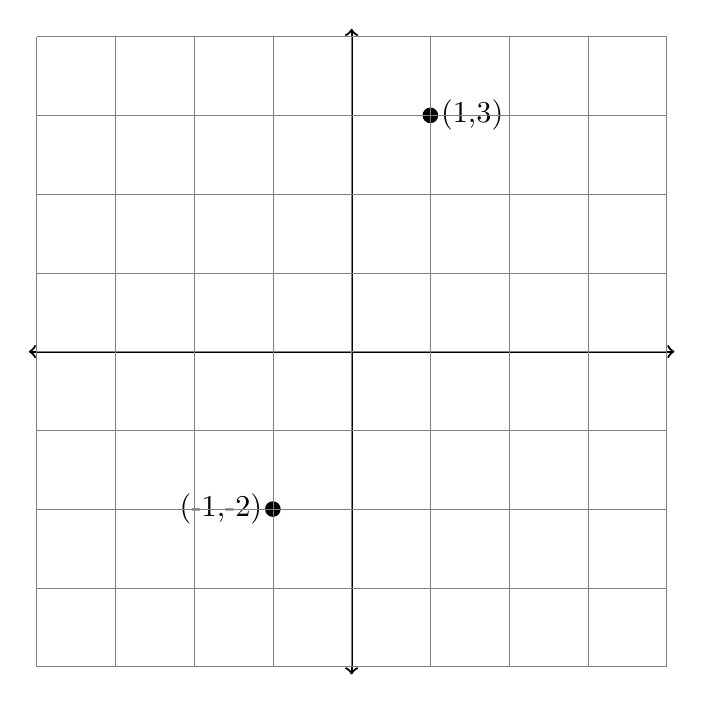
\begin{tikzpicture}
  % axis
  \draw[thick, <->] (0, -4.1) -- (0, 4.1);
  \draw[thick, <->] (-4.1, 0) -- (4.1, 0);
  \coordinate [circle, fill, inner sep=2pt] (a) at (-1,-2) ;
  \coordinate [circle, fill, inner sep=2pt] (b) at (1,3) ;
  \node [left] at (a) {(-1,-2)};
  \node [right] at (b) {(1,3)};
  % grid
  \draw[help lines, step = 1cm] (-4, -4) grid (4, 4);
  
\end{tikzpicture}

We can draw a right triangle and use the Pythagorean Theorem:

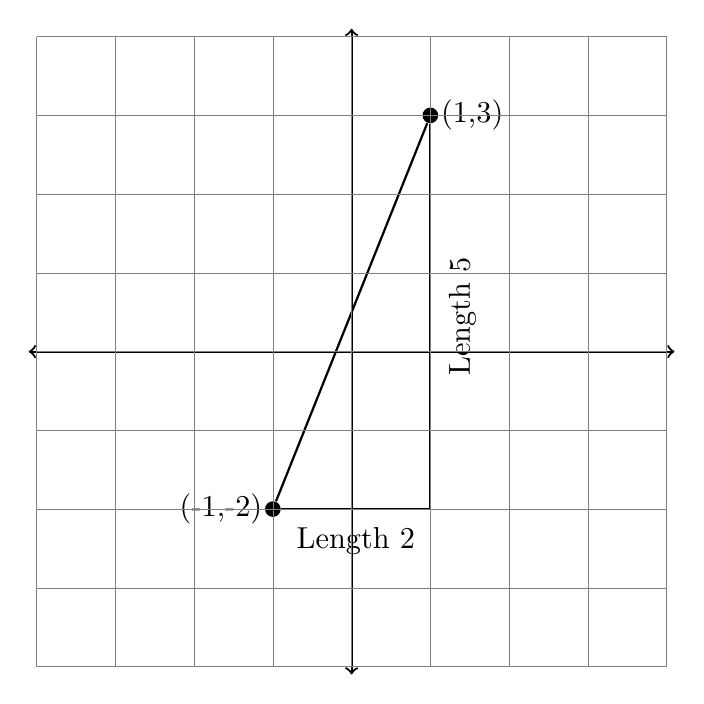
\begin{tikzpicture}
  % axis
  \draw[thick, <->] (0, -4.1) -- (0, 4.1);
  \draw[thick, <->] (-4.1, 0) -- (4.1, 0);
  \coordinate [circle, fill, inner sep=2pt] (a) at (-1,-2) ;
  \coordinate [circle, fill, inner sep=2pt] (b) at (1,3) ;
    \node [left] at (a) {(-1,-2)};
  \node [right] at (b) {(1,3)};
  \coordinate (c) at (1, -2);

  \draw [thick] (a) -- (b);
  \draw [thick] (a) -- node[outer sep = 3pt, below]{Length 2}(c);
  \draw [thick] (c) -- node[rotate=90, outer sep = 3pt, below]{Length 5}(b);
  \draw[help lines, step = 1cm] (-4, -4) grid (4, 4);
 
\end{tikzpicture}


The distance between the two points is $\sqrt{2^2 + 5^2} = \sqrt{29}
\approx 5.385165$. In other words, you square the change in $x$ and add it to
the square of the change in $y$. The distance is the square root of
that sum.

\section{Distance in 3 Dimensions}

What if the point is in three-dimensional space?  For example, you move 2
meters East, 8 meters North, and 4 meters up in the air. How far are
you from where you started?  You just square each, sum them, and take the square root:
$\sqrt{2^2 + 8^2 + 4^2} = \sqrt{84} = 2\sqrt{21} \approx 9.165$ meters.\index{distance!in 3 dimensions}

\begin{tikzpicture}
  \draw [thick, ->] (0,0,0) -- (9,0,0) node[outer sep = 1pt, right]{North} ; 
  \draw [thick, ->]  (0,0,0) -- (0,3,0) node[outer sep = 1pt, above]{Up} ; 
  \draw [thick, ->] (0,0,0) -- (0,0,4) node[outer sep = 1pt, below]{East} ; 

    \draw [dashed]  (8,0,0) -- node[outer sep = 1pt, right]{2}  (8,0,2); 

  \draw [dashed]  (0,0,2) -- node[outer sep = 1pt, below]{8} (8,0,2); 
  \draw [dashed]  (8,0,2) -- node[outer sep = 1pt, right]{4} (8,4,2); 
  \draw [thick]  (0,0,0) --  (8,4,2) node[circle, fill, inner sep=2pt]{}; 
  \node [left] at (5, 2.7, 1){$\sqrt{2^2 + 8^2 + 4^2} \approx 9.165$};

\end{tikzpicture}

This leads us to a formal definition of the distance formula:
\[
d = \sqrt{(x_2 - x_1)^2 + (y_2 - y_1)^2}
\]
Or in 3D space:
\[
d = \sqrt{(x_2 - x_1)^2 + (y_2 - y_1)^2 + (z_2 - z_1)^2}
\]

\graphicspath{{../../Chapters/congruence/en_US}}
\chapter{Congruence}
% Add: simple triangles
%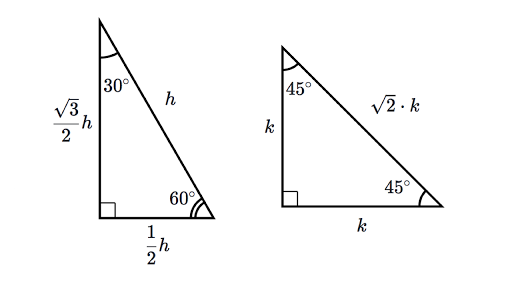
\includegraphics[width=0.8\textwidth]{KA_Special_Triangles.png}
Look at this picture of two geometric figures.

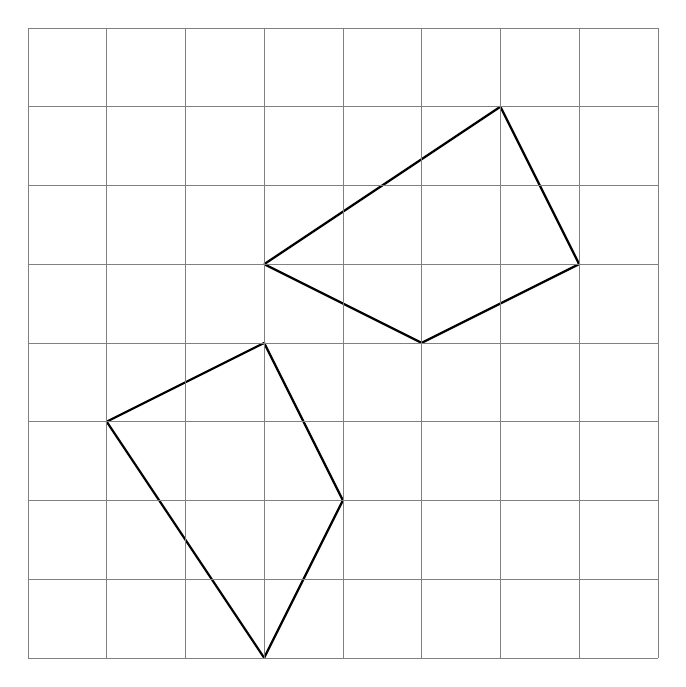
\begin{tikzpicture}
 
  	\draw [thick] (-1,-4) --  (0, -2);
	\draw [thick] (0,-2) --  (-1, 0) ;
	\draw [thick] (-1,0) --  (-3, -1); 
	\draw [thick] (-3,-1) --  (-1, -4);
	
	\draw [thick] (-1,1) --  (1, 0);
	\draw [thick] (1,0) --  (3, 1) ;
	\draw [thick] (3,1) --  (2, 3); 
	\draw [thick] (2,3) --  (-1, 1);

  \draw[help lines, step = 1cm] (-4, -4) grid (4, 4);
 
\end{tikzpicture}

They are the same shape, right? If you cut one out with scissors, it
would lay perfectly on top of the other. In geometry, we say they are
\emph{congruent}.

What is the official definition of ``congruent''? 
Two geometric figures are congruent if you can transform one into the other using
only rigid transformations. 

You might be wondering now, what are rigid transformations?
A transformation is \emph{Rigid} if it doesn't change the distances
between the points or the measure of the angles between the lines, they
form. These are all rigid transformations:
\begin{itemize}
\item Translations
\item Rotations
\item Reflections 
\end{itemize}

Once again imagine cutting out one figure with scissors and trying to match it with the second figure, your actions are rigid transformations:
\begin{itemize}
\item Translations - sliding the cutout left and right and up and down
\item Rotations	- rotating the cutout clockwise and counterclockwise
\item Reflection - flipping the piece of paper over
\end{itemize}

A transformation is rigid if it is some combination of translations, rotations, and reflections.

\section{Triangle Congruency}

If the sides of two triangles have the same length, the triangles must be congruent:

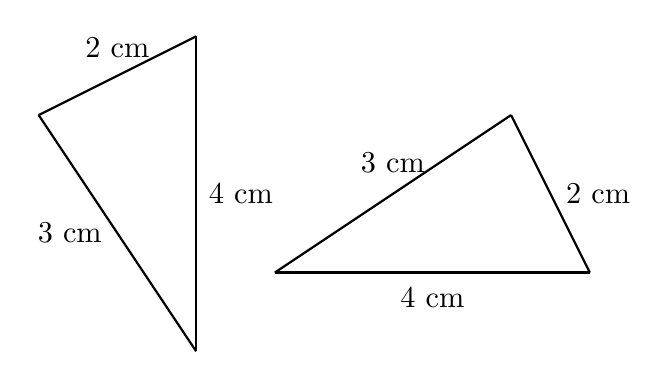
\begin{tikzpicture} 
  	\draw [thick] (-2,0) -- node[outer sep = 1pt, right]{4 cm}  (-2, 4) ;
	\draw [thick] (-2,4) --  node[outer sep = 3pt, above]{2 cm} (-4, 3); 
	\draw [thick] (-4,3) --  node[outer sep = 2pt, left]{3 cm} (-2, 0);
	
	\draw [thick] (-1,1) --  node[outer sep = 2pt, below]{4 cm}  (3, 1) ;
	\draw [thick] (3,1) --  node[outer sep = 2pt, right]{2 cm} (2, 3); 
	\draw [thick] (2,3) --  node[outer sep = 4pt, above]{3 cm} (-1, 1);
\end{tikzpicture}

To be precise, the Side-Side-Side Congruency Test says that two triangles are
congruent if three sides in one triangle are the same length as the
corresponding sides in the other. We usually refer to this as the SSS test.
% Explain with a^2 + b^2 = c^2

Note that two triangles with all three angles equal are not necessarily congruent.
For example, here are two triangles with the same interior angles, but they are
different sizes:

\begin{tikzpicture}
  \coordinate [circle, fill, inner sep=1pt] (a1) at (0,0) ;
  \coordinate [circle, fill, inner sep=1pt] (b1) at (4,0) ;
  \coordinate [circle, fill, inner sep=1pt] (c1) at (3,2) ;
  
   \coordinate [circle, fill, inner sep=1pt] (a2) at (5,0) ;
  \coordinate [circle, fill, inner sep=1pt] (b2) at (11,0) ;
  \coordinate [circle, fill, inner sep=1pt] (c2) at (9.5,3) ;
        \draw (a1) --   (b1);
        \draw (b1) -- (c1);
        \draw (c1)--  (a1);
        \pic [draw, "$63^\circ$", angle eccentricity=1.5] {angle = c1--b1--a1};
        \pic [draw, "$34^\circ$", angle eccentricity=2.0] {angle = b1--a1--c1};
        \pic [draw, "$83^\circ$", angle eccentricity=1.5] {angle = a1--c1--b1};

       \draw (a2) --  (b2);
        \draw (b2) -- (c2);
        \draw (c2)--  (a2);
        \pic [draw, "$63^\circ$", angle eccentricity=1.5] {angle = c2--b2--a2};
        \pic [draw, "$34^\circ$", angle eccentricity=2.0] {angle = b2--a2--c2};
        \pic [draw, "$83^\circ$", angle eccentricity=1.5] {angle = a2--c2--b2};

\end{tikzpicture}

These triangles are not congruent, but they are \emph{similar}. Meaning
 they have the same shape, but are not necessarily the same
size.

Therefore, if you know two angles of a triangle, you can calculate the third. So it makes sense
to say ``If two triangles have two angles that are equal, they are
similar triangles.''  And if two similar triangles have one side that
is equal in length, they must be the same size -- so they are
congruent. Thus, the Side-Angle-Angle Congruency Test says that
two triangles are congruent if two angles and one side match.

What if you know that two triangles have two sides that are the same
length and that the angle between them is also equal?

\begin{tikzpicture}
  \coordinate [circle, fill, inner sep=1pt] (a1) at (0,0) ;
  \coordinate [circle, fill, inner sep=1pt] (b1) at (4,0) ;
  \coordinate [circle, fill, inner sep=1pt] (c1) at (3,2) ;
  
  \coordinate [circle, fill, inner sep=1pt] (a2) at (5,0) ;
  \coordinate [circle, fill, inner sep=1pt] (b2) at (9,0) ;
  \coordinate [circle, fill, inner sep=1pt] (c2) at (8,2) ;
  
  \draw (a1) --  node[outer sep = 0.5pt, below]{4}  (b1);
  \draw [dashed] (b1) -- (c1);
  \draw (c1)--  node[outer sep = 5pt, above]{3.5} (a1);
  \pic [draw, "$34^\circ$", angle eccentricity=2.0] {angle = b1--a1--c1};

  \draw (a2) --  node[outer sep = 0.5pt, below]{4}  (b2);
  \draw [dashed] (b2) -- (c2);
  \draw (c2)--  node[outer sep = 5pt, above]{3.5} (a2);
  \pic [draw, "$34^\circ$", angle eccentricity=2.0] {angle = b2--a2--c2};
\end{tikzpicture}

Yes, they must be congruent. This is the Side-Angle-Size Congruency Test.

What if the angle isn't the one between the two known sides? If it is
a right angle, you can be certain the two triangles are congruent.
(How do I know? Because the Pythagorean Theorem tells us that we can
calculate the length of the third side. There is only one possibility,
thus all three sides must be the same length.)

\begin{tikzpicture}
  \coordinate [circle, fill, inner sep=1pt] (a1) at (0,0) ;
  \coordinate [circle, fill, inner sep=1pt] (b1) at (4,0) ;
  \coordinate [circle, fill, inner sep=1pt] (c1) at (4,2) ;
  
   \coordinate [circle, fill, inner sep=1pt] (a2) at (5,0) ;
  \coordinate [circle, fill, inner sep=1pt] (b2) at (9,0) ;
  \coordinate [circle, fill, inner sep=1pt] (c2) at (9,2) ;
        \draw (a1) --  node[outer sep = 0.5pt, below]{3.5}  (b1);
        \draw [dashed] (b1) -- (c1);
        \draw (c1)--  node[outer sep = 5pt, above]{4} (a1);
        \pic [draw] {right angle = a1--b1--c1};

        \draw (a2) --  node[outer sep = 0.5pt, below]{3.5}  (b2);
        \draw [dashed] (b2) -- (c2);
        \draw (c2)--  node[outer sep = 5pt, above]{4} (a2);
        \pic [draw] {right angle = a2--b2--c2};
\end{tikzpicture}

In this case, the third side of each triangle must be $\sqrt{4^2 - 3.5^2} \approx 1.9$.

What if the know angle is less than $90^\circ$? \emph{The triangles
  are not necessarily congruent.} For example, let's say that there are
two triangles with sides of length 5 and 7 and that the corresponding
angle (at the end of the side of length 7) on each is $45^\circ$. Two
different triangles satisfy this:

\begin{tikzpicture}
  \coordinate [circle, fill, inner sep=1pt] (a1) at (0,0) ;
  \coordinate [circle, fill, inner sep=1pt] (b1) at (7,0) ;
  \coordinate [circle, fill, inner sep=1pt] (c1) at (4,3) ;
  \coordinate [circle, fill, inner sep=1pt] (a2) at (8,0) ;
  \coordinate [circle, fill, inner sep=1pt] (b2) at (15,0) ;
  \coordinate [circle, fill, inner sep=1pt] (c2) at (11,4) ;
  \draw (a1) --  node[outer sep = 0.5pt, below]{7}  (b1);
  \draw [dashed] (b1) -- (c1);
  \draw (c1)--  node[outer sep = 5pt, above]{5}(a1);
  \pic [draw, "$45^\circ$", angle eccentricity=1.5] {angle = c1--b1--a1};
  \draw (a2) --  node[outer sep = 0.5pt, below]{7}  (b2);
  \draw [dashed] (b2) -- (c2);
  \draw (c2)--  node[outer sep = 5pt, above]{5} (a2);
  \pic [draw, "$45^\circ$", angle eccentricity=1.5] {angle = c2--b2--a2};
\end{tikzpicture}

Let's see this another way by laying one triangle on top of the other:

\begin{tikzpicture}
  \coordinate [circle, fill, inner sep=1pt] (a1) at (0,0) ;
  \coordinate [circle, fill, inner sep=1pt] (b1) at (7,0) ;
  \coordinate [circle, fill, inner sep=1pt] (c1) at (4,3) ;
  \coordinate [circle, fill, inner sep=1pt] (c2) at (3,4) ;
  \coordinate (d) at (2,5);
  \coordinate (e) at (3.5,3.5);

  \draw (a1) --  node[outer sep = 0.5pt, below]{7}  (b1);
  \draw [dashed,->] (b1) -- (d);
  \draw [dashed] (a1) -- (e);
  \draw (c1)--  node[outer sep = 5pt, below]{5}(a1);
  \draw (c2)--  node[outer sep = 5pt, above]{5}(a1);
  \pic [draw, "$45^\circ$", angle eccentricity=1.5] {angle = c1--b1--a1};
   \pic [draw, angle radius=8] {right angle = b1--e--a1};
\end{tikzpicture}


So there is \emph{not} a general Side-Side-Angle Congruency Test.

Here, then, is the list of common congruency tests:
\begin{itemize}
\item Side-Side-Side: All three sides have the same measure
\item Side-Angle-Angle: Two angles and one side have the same measure
\item Side-Angle-Side: Two sides and the angle between them have the same measure
\item Side-Side-Right: They are right triangles and have two sides have the same measure
\end{itemize}

\begin{Exercise}[title={Congruent Triangles}, label=con_triangles]
  Ted is terrible at drawing triangles: he always draws them exactly
  the same. Fortunately, he has marked these diagrams with the sides
  and angles that he measured. For each pair of triangles, write if
  you know them to be congruent and which congruency test proves
  it. For example:

\begin{tikzpicture}[scale=0.7]
  \coordinate [circle, fill, inner sep=1pt] (a1) at (0,1) ;
  \coordinate [circle, fill, inner sep=1pt] (b1) at (5,0) ;
  \coordinate [circle, fill, inner sep=1pt] (c1) at (4,2) ;
  
  \coordinate [circle, fill, inner sep=1pt] (a2) at (6,1) ;
  \coordinate [circle, fill, inner sep=1pt] (b2) at (11,0) ;
  \coordinate [circle, fill, inner sep=1pt] (c2) at (10,2) ;
  \draw (a1) --  node[outer sep = 0.5pt, below]{3.5}  (b1);
  \draw (b1) -- node[outer sep = 2pt, right]{4} (c1);
  \draw (c1)--  node[outer sep = 2pt, above]{} (a1);
  \pic [draw,  "$120^\circ$", angle eccentricity=2.0] {angle = c1--b1--a1};

  \draw (a2) --  node[outer sep = 0.5pt, below]{3.5}  (b2);
  \draw  (b2) -- node[outer sep = 2pt, right]{4} (c2);
  \draw (c2) -- node[outer sep = 2pt, above]{} (a2);
  \pic [draw,  "$120^\circ$",, angle eccentricity=2.0] {angle = c2--b2--a2};
\end{tikzpicture}

  (These drawings are clearly not accurate, but you are told the measurements are.) The answer is ``Congruent by the Side-Angle-Side test.''

  \begin{multicols}{2}

\begin{tikzpicture}[scale=0.6]
  \coordinate [circle, fill, inner sep=1pt] (a1) at (0,1) ;
  \coordinate [circle, fill, inner sep=1pt] (b1) at (5,0) ;
  \coordinate [circle, fill, inner sep=1pt] (c1) at (4,2) ;
  
  \coordinate [circle, fill, inner sep=1pt] (a2) at (6,1) ;
  \coordinate [circle, fill, inner sep=1pt] (b2) at (11,0) ;
  \coordinate [circle, fill, inner sep=1pt] (c2) at (10,2) ;
  \draw (a1) --  node[outer sep = 0.5pt, below]{3.5}  (b1);
  \draw (b1) -- node[outer sep = 2pt, right]{} (c1);
  \draw (c1)--  node[outer sep = 2pt, above]{6} (a1);
  \pic [draw,  "$90^\circ$", angle eccentricity=2.0] {angle = c1--b1--a1};

  \draw (a2) --  node[outer sep = 0.5pt, below]{3.5}  (b2);
  \draw  (b2) -- node[outer sep = 2pt, right]{} (c2);
  \draw (c2) -- node[outer sep = 2pt, above]{6} (a2);
  \pic [draw,  "$90^\circ$",, angle eccentricity=2.0] {angle = c2--b2--a2};
\end{tikzpicture}

\hspace{3cm}

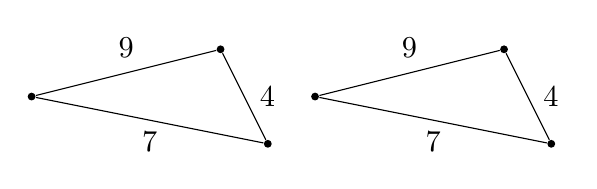
\begin{tikzpicture}[scale=0.6]
  \coordinate [circle, fill, inner sep=1pt] (a1) at (0,1) ;
  \coordinate [circle, fill, inner sep=1pt] (b1) at (5,0) ;
  \coordinate [circle, fill, inner sep=1pt] (c1) at (4,2) ;
  
  \coordinate [circle, fill, inner sep=1pt] (a2) at (6,1) ;
  \coordinate [circle, fill, inner sep=1pt] (b2) at (11,0) ;
  \coordinate [circle, fill, inner sep=1pt] (c2) at (10,2) ;
  \draw (a1) --  node[outer sep = 0.5pt, below]{7}  (b1);
  \draw (b1) -- node[outer sep = 2pt, right]{4} (c1);
  \draw (c1)--  node[outer sep = 2pt, above]{9} (a1);

  \draw (a2) --  node[outer sep = 0.5pt, below]{7}  (b2);
  \draw  (b2) -- node[outer sep = 2pt, right]{4} (c2);
  \draw (c2) -- node[outer sep = 2pt, above]{9} (a2);
\end{tikzpicture}


\begin{tikzpicture}[scale=0.6]
  \coordinate [circle, fill, inner sep=1pt] (a1) at (0,1) ;
  \coordinate [circle, fill, inner sep=1pt] (b1) at (5,0) ;
  \coordinate [circle, fill, inner sep=1pt] (c1) at (4,2) ;
  
  \coordinate [circle, fill, inner sep=1pt] (a2) at (6,1) ;
  \coordinate [circle, fill, inner sep=1pt] (b2) at (11,0) ;
  \coordinate [circle, fill, inner sep=1pt] (c2) at (10,2) ;
  \draw (a1) --  node[outer sep = 0.5pt, below]{7}  (b1);
  \draw (b1) -- node[outer sep = 2pt, right]{} (c1);
  \draw (c1)--  node[outer sep = 2pt, above]{} (a1);
  \pic [draw,  "$35^\circ$",, angle eccentricity=2.0] {angle = c1--b1--a1};
  \pic [draw,  "$62^\circ$",, angle eccentricity=2.0] {angle = b1--a1--c1};

  \draw (a2) --  node[outer sep = 0.5pt, below]{7}  (b2);
  \draw  (b2) -- node[outer sep = 2pt, right]{} (c2);
  \draw (c2) -- node[outer sep = 2pt, above]{} (a2);
  \pic [draw,  "$35^\circ$",, angle eccentricity=2.0] {angle = c2--b2--a2};
  \pic [draw,  "$62^\circ$",, angle eccentricity=2.0] {angle = b2--a2--c2};

\end{tikzpicture}

\hspace{3cm}


\begin{tikzpicture}[scale=0.6]
  \coordinate [circle, fill, inner sep=1pt] (a1) at (0,1) ;
  \coordinate [circle, fill, inner sep=1pt] (b1) at (5,0) ;
  \coordinate [circle, fill, inner sep=1pt] (c1) at (4,2) ;
  
  \coordinate [circle, fill, inner sep=1pt] (a2) at (6,1) ;
  \coordinate [circle, fill, inner sep=1pt] (b2) at (11,0) ;
  \coordinate [circle, fill, inner sep=1pt] (c2) at (10,2) ;
  \draw (a1) --  node[outer sep = 0.5pt, below]{8}  (b1);
  \draw (b1) -- node[outer sep = 2pt, right]{6} (c1);
  \draw (c1)--  node[outer sep = 2pt, above]{} (a1);
  \pic [draw,  "$28^\circ$",, angle eccentricity=2.0] {angle = b1--a1--c1};

  \draw (a2) --  node[outer sep = 0.5pt, below]{8}  (b2);
  \draw  (b2) -- node[outer sep = 2pt, right]{6} (c2);
  \draw (c2) -- node[outer sep = 2pt, above]{} (a2);
  \pic [draw,  "$28^\circ$",, angle eccentricity=2.0] {angle = b2--a2--c2};

\end{tikzpicture}


\end{multicols}
\end{Exercise}

\begin{Answer}[ref=con_triangles]
\begin{multicols}{2}
Congruent by the Side-Side-Right Congruency Test.

Congruent by the Side-Side-Side Congruency Test.

Congruent by the Side-Angle-Angle Congruency Test.

We don't know if they are congruent. The measured angle is not between the measured sides.

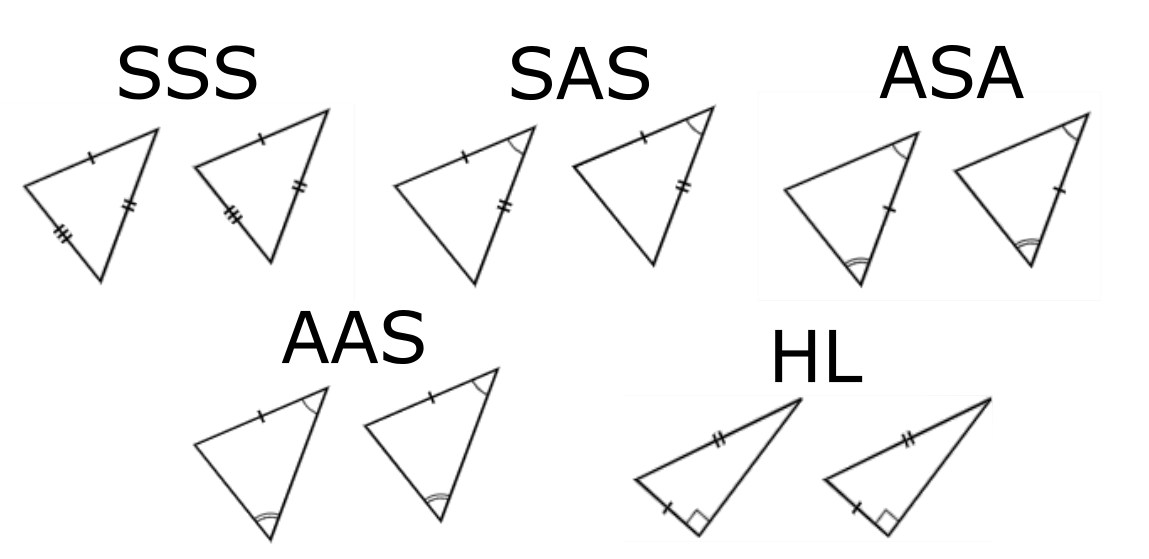
\includegraphics[width=0.8\textwidth]{Triangle_Congruence.png}
\end{multicols}

\end{Answer}




\graphicspath{{../../Chapters/parallel_perpendicular/en_US}}
\chapter{Parallel and Perpendicular}

Two vectors are said to be parallel if they have the same or opposite
direction. In simpler terms, if two vectors are pointing in the same
direction (even if their magnitudes differ), they are considered
parallel. For example, imagine you have a vector representing the
direction and speed of a car moving north. If you have another vector
representing the direction and speed of a different car also moving
north, these vectors are parallel.\index{parallel}

On the other hand, if two vectors point in completely opposite
directions, they are still considered parallel. For instance, if one
vector represents a car moving north and the other represents a car
moving south, these vectors are parallel but in opposite directions.

Perpendicular vectors, as the name suggests, are vectors that
intersect each other at a right angle, forming a 90-degree angle. If
we imagine a sheet of paper, drawing a horizontal vector and a
vertical vector on that paper would create perpendicular vectors. In
this case, the horizontal vector represents left-right direction,
while the vertical vector represents up-down direction. Perpendicular
vectors are often seen in geometric shapes, such as squares and
rectangles, where their sides intersect at right angles.\index{perpendicular}

A fundamental property of perpendicular vectors is that their dot
product is zero. The dot product is a mathematical operation that
measures the extent to which two vectors align with each other. When
two vectors are perpendicular, their dot product is always zero. This
property provides a useful tool for determining whether two given
vectors are perpendicular.

Understanding parallel and perpendicular vectors is essential in
various areas of mathematics and physics. For example, in geometry,
knowledge of perpendicular vectors helps us determine whether lines
are perpendicular or parallel. In physics, vectors can represent
forces, velocities, or displacements, and identifying parallel or
perpendicular vectors aids in analyzing motion and forces acting on
objects.

In summary, parallel vectors have the same or opposite direction,
while perpendicular vectors intersect at a right angle. Recognizing
these relationships between vectors enables us to solve problems
involving geometry, physics, and many other fields. As you delve
deeper into the exciting world of vectors, keep an eye out for
parallel and perpendicular relationships, as they often hold valuable
insights and solutions.

\graphicspath{{../../Chapters/circles/en_US}}
\chapter{Circles}

A circle is the set of points $(x, y)$ that are a particular distance $r$ from a
particular point $(x_c, y_c)$.  We say that $r$ is the
\newterm{radius} and $(x_c, y_c)$ is the \newterm{center}

\begin{tikzpicture}
    \filldraw [sdkblue] (1,2) circle (2pt) node[anchor=west]{$(x_c, y_c)$};
    \filldraw [sdkblue] (2,4.82842712474619) circle (2pt) node[anchor=west]{
    $(x, y)$};
    \draw [sdkblue,dashed](1,2) -- (2,4.82842712474619) node[midway,anchor=
    west] {$r$};
    \draw [sdkblue](1,2) circle (3);
    \draw [stealth-stealth](-2.5,0)--(4.5,0);
    \draw [stealth-stealth](0,-1.5)--(0,5.5);
\end{tikzpicture}

\begin{mdframed}[style=important, frametitle={Area and Radius}]

  If the radius of a circle is $r$, the area of its interior ($a$) is given 
  by \index{circle!area of}

  $$a = \pi r^2$$

\end{mdframed}

\begin{Exercise}[title={Area of a Circle}, label=area_of_circle]

  The paint you have says ``One liter covers 6 square meters.''

  You are painting the top of a circular table with a radius of 3 meters.

  How much paint will you need?
  
\end{Exercise}
\begin{Answer}[ref=area_of_circle]

  The table has a radius of 3 meters.

  So the area of its top is $3^2 \pi \approx 28.27$.

  $$ 28.27 \text{ square meters }\left(\frac{1 \text{ liter }}{6 \text{ square 
  meters }} \right) = 4.72 \text{ liters }$$ 
  
\end{Answer}


Note that a circle lives in a particular plane. The points $(x, y, z)$ that 
are a particular distance $r$ from a particular point $(x_c, y_c, z_c)$ are a 
sphere:

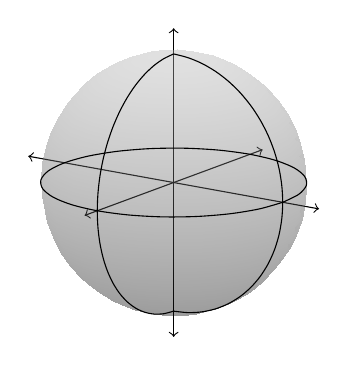
\begin{tikzpicture}
  \begin{axis}[
    view={35}{15},
    unit vector ratio=1 1 1,
    ticks = none,
    axis lines=middle,
    ymin=-3.5,
    ymax=3.5,
    xmax=4.0,
    xmin=-4.0,
    zmin=-3.6,
    zmax=3.6,
    x axis line style=<->,
    y axis line style=<->,
    z axis line style=<->,
    clip=false
    ]
    \addplot3[surf,shader=interp,domain=0:360,y domain=-90:90, opacity=0.4,
    colormap={blackwhite}{color=(black) color=(black!30)}] ({3 * cos(y) * 
    cos(x)},
    {3 *  cos(y) * sin(x)},{3 * sin(y)});
    \addplot3[samples y=0,domain=0:360,smooth]({3*cos(x)}, {3*sin(x)}, 0.0);
    \addplot3[samples y=0,domain=-180:0,smooth](0, {3*sin(x)}, {3*cos(x)});
    \addplot3[samples y=0,domain=0:180,smooth]({3*sin(x)}, 0, {3*cos(x)});
  \end{axis}
\end{tikzpicture}

The distance all the way across the middle of a circle (or a sphere) is its
\newterm{diameter}.  The diameter is always twice the radius.

For the rest of the chapter, we are talking about circles, points, and
lines \textit{in a plane}.

\begin{mdframed}[style=important, frametitle={Circumference and Diameter}]

  The circumference ($c$) of a circle is the distance around the circle. If the
  diameter is $d$, \index{circumference}

  $$c = \pi d$$

\end{mdframed}

\begin{Exercise}[title={Circumference}, label=circumference]

  Using a tape measure, you figure out that the circumference of a tree in your
  yard is 64 cm.

  Assuming the trunk is basically circular,  what is its diameter?
  
\end{Exercise}
\begin{Answer}[ref=circumference]

  The diameter is $$\frac{c}{\pi} = \frac{64}{\pi} \approx 20.37 \text{ 
  centimeters}$$
  
\end{Answer}
\begin{Exercise}[title={Splitting a Pie}, label=pie_splitting]

  A pie has a radius of 13 cm.  7 friends all want equal sized wedges.  You 
  have a tape measure.

  How many centimeters will each outer crust be?

\end{Exercise}
\begin{Answer}[ref=pie_splitting]

  The circumference of the pie is $26 \pi \approx 81.7$ centimenters.
  
  The length of the crust for each piece would be about $\frac{81.7}{7} = 11.7$
  cm.

  
\begin{tikzpicture}
    \filldraw [black] (0,0) circle (2pt);
    \draw [black](0,0) circle (3);
    \foreach \x in {0,...,6}
    \draw [dashed] (0,0) -- ({3 * cos(\x * 51.428571428571429)}, {3 * sin(\x 
    * 51.428571428571429)});
    \draw [sdkblue,very thick] (3, 0) arc (0:51.43:3) node [midway, anchor=east] 
    {11.7 cm};
    \node at (1.0, 1.5)  {13 cm};
\end{tikzpicture}
\end{Answer}



\begin{mdframed}[style=important, frametitle={Length of an Arc}]

If you have two points $a$ and $b$ on a circle, the ray from the
center through $a$ and the ray from the center through $b$ form an
angle.  If $\theta$ is the angle in radians and $r$ is the radius of
the circle, the distance from $a$ to $b$ on the circle is $r \theta$.

\begin{tikzpicture}
    \filldraw [black] (0,0) circle (2pt) node[anchor=west]{Center};
    \filldraw [sdkblue] (-1,2.82842712474619) circle (2pt) node[anchor=west]{$b$};
    \filldraw [sdkblue] (2.12132,2.12132) circle (2pt) node[anchor=east]{$a$};
    \draw [sdkblue,dashed,->](0,0) -- (-1.2,3.394112549695428);
    \draw [sdkblue,dashed,->](0,0) -- (2.4, 2.4) node[midway,anchor=east]{$r$};
    \draw [black](0,0) circle (3);
    \draw [sdkblue,very thick] (2.12132,2.12132) arc (45:109.47:3) node [midway, 
    anchor=south] {$r \theta$};
    \draw [sdkblue, <->] (0.707,0.707) arc (45:109.47:1) node [midway, 
    anchor=south]{$\theta$};
\end{tikzpicture}

\end{mdframed}

\begin{Exercise}[title={Arc Length}, label=arc_length]

You have been asked to find the radius of a very large cylindrical tank.
You have a tape measure, but it is only 15 meters long and doesn't
reach all the way around the tank.

However, you have a compass.  So you stick one end of the tape measure
to the side of the tank and measure the orientation of the wall at
that point.  Then you walk the 15 meters and measure the orientation of the 
wall there.

You find that 15 meters represents 72 degrees of arc.

What is the radius of the tank in meters?
  
\end{Exercise}
\begin{Answer}[ref=arc_length]

  $$72 \text{ degrees } \left(\frac{2\pi \text{ radians }}{360 \text{ degrees }
  }\right) \approx 1.2566 \text{ radians }$$

  $$15 = 1.2566r$$

  $$r = 11.94 \text{ meters}$$
  
\begin{tikzpicture}
    \filldraw [black] (0,0) circle (2pt);
    \draw [black](0,0) circle (3);
    \draw [dashed] (0,0) -- ({3 * cos(72)}, {3 * sin(72)});
    \draw [dashed] (0,0) -- (3, 0);
    \draw [sdkblue,very thick] (3,0) arc (0:72:3) node [midway, anchor=east] 
    {15 m};
    \draw [sdkblue, <->] (1,0) arc (0:72:1) node [midway, anchor=east]{$72^
    \circ$ = 1.2566 rad};
    \node at (0.0, 1.6)  {11.94 m};
\end{tikzpicture}
\end{Answer}

\section{Tangents}

A line that is \newterm{tangent} to a circle touches it at exactly one point:

\begin{tikzpicture}
    \filldraw [black] (0,0) circle (2pt);
    \draw [dashed, black](0,0) circle (3);
    \filldraw [sdkblue] (2.121, 2.121) circle (2pt);
    \draw [sdkblue, thick] (6.243, -2) -- (0, 4.243);
\end{tikzpicture}

The tangent line is always perpendicular to the radius to the point of tangency:

\begin{tikzpicture}
  \filldraw [black] (0,0) circle (2pt);
  \draw [dashed, black](0,0) circle (3);
  \filldraw [sdkblue] (2.121, 2.121) circle (2pt);
  \draw [sdkblue, thick] (0,0) -- (2.121, 2.121);
  \draw [black] (1.9, 1.9) -- (2.121, 1.679) -- (2.342,1.9);
  \draw [sdkblue, thick] (6.243, -2) -- (0, 4.243);
\end{tikzpicture}


\begin{Exercise}[title={Painting a Comet}, label=painting_comet]
  
  You have been asked to paint a comet and its tail in yellow on the floor of a 
  gymnasium.

  A liter of yellow paint covers 6 square meters.

  First you draw a circle with a radius of 3 meters.  Then you mark a
  point $D$ on the floor 7 meters from the center of the circle.  Then
  you draw two tangent lines that pass through $D$.

  You use a protractor to measure the angle at which the tangent lines meet: about 
  $51^\circ$
  
  \begin{tikzpicture}
    \filldraw [sdkblue] (0,0) circle (2pt);
    \filldraw [black] (7,0) circle (2pt);
    \draw [sdkblue,dashed] (0,0) -- (3,0) node [midway, anchor=south] {3 m};
    \draw [sdkblue,dashed] (3,0) -- (7,0) node [midway, anchor=south] {4 m};
    \draw [sdkblue,dashed, ->] (5.5,0) arc (180:154.6:1.5) node [midway, 
    anchor=west]{$51^\circ$};
    \draw [sdkblue,dashed, ->] (5.5,0) arc (180:205.4:1.5);
    \draw [black,thick] (7,0) -- ({3 * cos(64.62)}, {3 * sin(64.62)});
    \draw [black,thick] (7,0) -- ({3 * cos(-64.62)}, {3 * sin(-64.62)});
    \filldraw [black] ({3 * cos(64.62)}, {3 * sin(64.62)}) circle (2pt);
    \filldraw [black] ({3 * cos(-64.62)}, {3 * sin(-64.62)}) circle (2pt);
    \filldraw [sdkblue] (3, 0) circle (2pt);
    \draw [sdkblue,dashed] ({3 * cos(-64.62)}, {3 * sin(-64.62)}) arc 
    (-64.62:64.62:3);
    \draw [black,thick] ({3 * cos(64.62)}, {3 * sin(64.62)}) arc 
    (64.62:295.38:3);
  \end{tikzpicture}

  Before you paint the area contained by the circle and the two
  tangent lines, how much paint will you need?
    

\end{Exercise}
\begin{Answer}[ref=painting_comet]

  The trick here is to take advantage of the fact that the tangent is 
  perpendicular to the radius to make right triangles:

  \begin{tikzpicture}
    \coordinate (a) at ({3 * cos(64.62)}, {3 * sin(64.62)});
    \coordinate (b) at ({3 * cos(-64.62)}, {3 * sin(-64.62)});
    \filldraw [sdkblue] (0,0) circle (2pt);
    \filldraw [black] (7,0) circle (2pt);
    \draw [black,thick] (0,0) -- (a) node [midway, anchor=east] {3m};
    \draw [black,thick] (0,0) -- (b) node [midway, anchor=east] {3m};
    \draw [black,thick] (0,0) -- (7,0) node [midway, anchor=south] {7 m};
    \draw [sdkblue,dashed, <->] (5.5,0) arc (180:154.6:1.5) node [midway, 
    anchor=west]{$25.5^\circ$};
    \draw [sdkblue,dashed, <->] (5.5,0) arc (180:205.4:1.5) node [midway, 
    anchor=west]{$25.5^\circ$};
    \draw [sdkblue,dashed, <->] (1.5,0) arc (0:64.5:1.5) node [midway, 
    anchor=west]{$64.5^\circ$};
    \draw [sdkblue,dashed, <->] (1.5,0) arc (0:-64.5:1.5) node [midway, 
    anchor=west]{$64.5^\circ$};
    \draw [black,thick] (7,0) -- (a);
    \draw [black,thick] (7,0) -- (b);
    \filldraw [black] (a) circle (2pt);
    \filldraw [black] (b) circle (2pt);
    \draw [black,thick] (a) arc (64.62:295.38:3);
  \end{tikzpicture}

  The wedge has radius 3 and represents $360 - 2(64.5) = 231^\circ \approx 4.03 
  \text{ radians}$.

  We are finding the area of this piece:
  
  \begin{tikzpicture}
    \coordinate (a) at ({3 * cos(64.62)}, {3 * sin(64.62)});
    \coordinate (b) at ({3 * cos(-64.62)}, {3 * sin(-64.62)});
    \filldraw [sdkblue] (0,0) circle (2pt);
    \draw [black,thick] (0,0) -- (a) node [midway, anchor=west] {3m};
    \draw [black,thick] (0,0) -- (b);
    \draw [sdkblue,dashed, <->] ({1.5 * cos(64.62)}, {1.5 * sin(64.62)}) arc 
    (64.5:295.5:1.5) node [midway]{4.03 rad};
    \filldraw [black] (a) circle (2pt);
    \filldraw [black] (b) circle (2pt);
    \draw [black,thick] (a) arc (64.62:295.38:3);
  \end{tikzpicture}

  The area of this piece is $(4.03)(3^2) = 36.27$ square meters.

  If a right triangle has a hypotenuse of 7m and one leg is 3m, the
  other leg is $\sqrt{7^2 - 3^2} = 2 \sqrt{10} \approx 6.3$ m.

    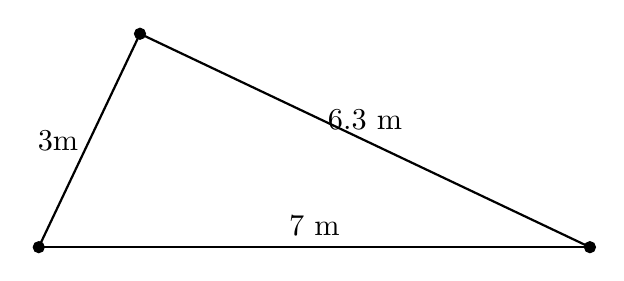
\begin{tikzpicture}
    \coordinate (a) at ({3 * cos(64.62)}, {3 * sin(64.62)});
    \filldraw [black] (7,0) circle (2pt);
    \filldraw [black] (0,0) circle (2pt);
    \draw [black,thick] (0,0) -- (a) node [midway, anchor=east] {3m};
    \draw [black,thick] (0,0) -- (7,0) node [midway, anchor=south] {7 m};
    \draw [black,thick] (7,0) -- (a) node [midway, anchor=south] {6.3 m};
    \filldraw [black] (a) circle (2pt);
  \end{tikzpicture}

  
  A right triangle with legs of 3m and 6.3m has an area of 9.45 square meters.

  There are two of them, so the total area is $36.27 + 2(18.9) = 74.07$ square 
  meters.

  Six square meters per liter, so you need $\frac{74.07}{6} = 12.35$ liters of 
  paint.

\end{Answer}

\section{Radians and circles}
Previously, you learned that angles can be measured in degrees and radians. A 
circle is $360^o$ (see figure \ref{fig:circledeg}). 

\begin{figure}[htbp]
\centering
\begin{tikzpicture}
        \begin{polaraxis}[axis lines = none, clip = false]
    \draw[black](0,0) -- (0, 3);
    \draw[black, dashed] (0,0) -- (180, 3);
    \addplot[blue, thick, domain = 0:360, samples = 200]{2.5};
    \addplot[red, domain = 0:175]{1};
    \draw[red, -latex](175, 1) -- (180,1);
    \addplot[red, domain = 180:355]{1};
    \draw[red, -latex] (355, 1) -- (360, 1);
    \node[] at (90, 1.5) {$\theta_1 = 180^\circ$};
    \node[] at (270, 1.5) {$\theta_2 = 180^\circ$};
    \end{polaraxis}
    \end{tikzpicture}
    \caption{The total internal angle of a circle is $\theta_1 + \theta_2 = 
    360^\circ$}
    \label{fig:circledeg}
\end{figure}

This means a circle is also $2\pi$ radians:
$$360^\circ \cdot \frac{\pi}{180^\circ} = 2\pi$$

You may have been wondering: why is it that there are $\pi$ radians in a 
$180^\circ$ angle? A radian is defined such that one radian is the angle at the 
center of a circle which defines an arc of the circumference equal to the 
radius of the circle (see figure \ref{fig:oneradian}). 

\begin{figure}[htbp]
\centering
\begin{tikzpicture}
        \begin{polaraxis}[axis lines = none, ymin = 0, ymax = 3, 
	clip = false]
 \addplot[blue, thick, domain = 0:360, samples = 300] {2.5};
 \addplot[red, thick, domain = 0:57.3] {2.5};
 \draw[red, thick](0,0) -- (0, 2.5);
 \draw[red, thick] (0,0) -- (57.3, 2.5);
 \addplot[red, domain = 0:57.3]{0.5};
 \addplot[black, domain = 0:57.3]{2.75};
 \draw[black](0,2.7) -- (0,2.8);
 \draw[black] (57.3, 2.7) -- (57.3, 2.8);
 \node[rotate = -60] at (27.5, 2.9) {\small length $= r$};
 \node[] at (27.5, 1) {\small $\theta = 1$};
    \end{polaraxis}
    \end{tikzpicture}
    \caption{When the center angle is 1 radian, the length of the arc is equal 
    to the radius of the circle}
    \label{fig:oneradian}
\end{figure} 

This makes it very straightforward to find the lengths of arcs if we know the 
center angle in radians. The arc length is just $\theta r$, where $\theta$ is 
the center angle in radians. 
\graphicspath{{../../Chapters/functions/en_US}}
\chapter{Functions and Their Graphs}

Functions are a major part of science, engineering, and math. You can think of a function as a machine: you put something into the
machine, it processes it, and out comes something else: a product. Just as we
often use the variable $x$ to stand in for a number, we often use the
variable $f$ to stand in for a function. $f(x)$ is said as ``f of x``.
% One of my teachers told me half of understanding math is understanding mathmaticions are just lazy, maybe a good add in somewhere

For example, we might ask, ``Let the function $f$ be defined like this:

\begin{equation*}
f(x) = -5x^2 + 12x + 2
\end{equation*}

What is the value of $f(3)$, said as ``f of 3``?

You would run the number 3 through ``the machine'': $-5(3^2) + 12(3) + 2 = -7$. The answer would be ``$f(3)$ is $7$''.

However, some functions are not defined for every possible input. For example:

\begin{equation*}
  f(x) = \frac{1}{x}
\end{equation*}

  This is defined for any $x$ except 0, because you can't divide 1 by 0. The set of values that a function can process is called its \textit{domain}, and resulting output values are called the range.
  It is important to note that functions have only one \emph{output} for each \emph{input}. However, multiple inputs can have the same output. 
  A relationship where one input can result in the more than one output is not a function, but a relation. This can be proven by the \hyperref[sec:vertical]{vertical line test}.
% some good images could be found here: https://www.ck12.org/book/ck-12-algebra-i-honors/section/3.1/ 

\begin{Exercise}[title={Domain of a function}, label=function_domain]

  Let the function $f$ be given by $f(x) = \sqrt{x - 3}$.  What is its domain?

\end{Exercise}
\begin{Answer}[ref=function_domain]
  You can only take the square root of nonnegative numbers, so the
  function is only defined when $x - 3 \geq 0$.  Thus, the domain is
  all real numbers greater than or equal to 3.
\end{Answer}

\section{Graphs of Functions}

If you have a function, $f$, its graph is the set of pairs $(x, y)$
such that $y = f(x)$.  We usually draw a picture of this set, called a \textit{graph}. 
The graph not only includes the picture, but also the values of x and y used to create it.

Here is the graph of the function $f(x) = -5x^2 + 12x + 2$:

\begin{tikzpicture}
    \begin{axis}[
        xmin=-1,xmax=3.5,
        ymin=-10,ymax=11,
        axis x line=middle,
        axis y line=middle,
        axis line style=<->,
        xlabel={$x$},
        ylabel={$y$},
        ]
        \addplot[no marks,sdkblue,<->] expression[domain=-0.7:3.05,samples=100]{(-5)*(x^2) + (12 * x) + 2}; 
    \end{axis}
\end{tikzpicture}

(Note that this is just part of the graph; it goes infinitely in both
directions. Remember your vectors!)

Here is the graph of the function $f(x) = \frac{1}{x}$:

\begin{tikzpicture}
    \begin{axis}[
        xmin=-7,xmax=7,
        ymin=-7,ymax=7,
        axis x line=middle,
        axis y line=middle,
        axis line style=<->,
        xlabel={$x$},
        ylabel={$y$},
        ]
        \addplot[no marks,sdkblue,<->] expression[domain=-6.5:-0.15,samples=100]{1/x}; 
        \addplot[no marks,sdkblue,<->] expression[domain=0.15:6.5,samples=100]{1/x}; 
    \end{axis}
\end{tikzpicture}
To draw a graph, take each x value (usually in increments of 1) and determine its corresponding y value. 
Then, plot those points on a graph, using the origin as the starting point. 
% do we assume students know how to graph?
\begin{Exercise}[title={Draw a graph}, label=draw_graph]

  Let the function $f$ be given by $f(x) = -3x + 3$. Sketch its graph.
% More space needed in exercise box
\end{Exercise}
\begin{Answer}[ref=draw_graph]

  The graph of this function is a line, its slope is -3, and it intersects the y axis at $(0, 3)$.

\begin{tikzpicture}
    \begin{axis}[
        xmin=-1,xmax=3,
        ymin=-7,ymax=7,
        xtick={1},
        ytick={3},
        axis x line=middle,
        axis y line=middle,
        axis line style=<->,
        xlabel={$x$},
        ylabel={$y$},
        ]
        \addplot[no marks,sdkblue,<->] expression[domain=-0.75:2.74,samples=100]{-3 * x + 3}; 
    \end{axis}
\end{tikzpicture}
  
  
\end{Answer}


\section{Can this be expressed as a function?}
\label{sec:vertical}

Note that not all sets can be expressed as graphs of functions.  For
example, here is the set of points $(x,y)$ such that $x^2 + y^2 = 9$:

\begin{tikzpicture}
    \begin{axis}[
        xmin=-3.5,xmax=3.5,
        ymin=-3.5,ymax=3.5,
        ytick={-3,-2,-1,0,1,2,3},
        axis x line=middle,
        axis y line=middle,
        axis line style=<->,
        xlabel={$x$},
        ylabel={$y$},
        ]
        \addplot[no marks,sdkblue] expression[domain=-3:3,samples=100]{sqrt(9 - x^2)}; 
        \addplot[no marks,sdkblue] expression[domain=-3:3,samples=100]{-1 * sqrt(9 - x^2)}; 
    \end{axis}
\end{tikzpicture}

This cannot be the graph of a function, because what would $f(0)$ be? 3
or -3?  This set fails what we call ``the vertical line test'': If any
vertical line contains more than one point from the set, it isn't the graph
of a function.  For example, the vertical line $x = 2$ would cross the graph twice:
\begin{center}
  
  \begin{tikzpicture}
    \begin{axis}[
      xmin=-3.5,xmax=3.5,
      ymin=-3.5,ymax=3.5,
      ytick={-3,-2,-1,0,1,2,3},
      axis x line=middle,
      axis y line=middle,
      axis line style=<->,
      xlabel={$x$},
      ylabel={$y$},
      ]
      \addplot[no marks,sdkblue] expression[domain=-3:3,samples=100]{sqrt(9 - x^2)}; 
      \addplot[no marks,sdkblue] expression[domain=-3:3,samples=100]{-1 * sqrt(9 - x^2)};
      \addplot [thick, dashed] coordinates {(2,-2.5)(2,2.5)};
      
    \end{axis}
    
  \end{tikzpicture}
\end{center}
%might be a good place to talk about even vs odd functions
\index{vertical line test}

\section{Inverses}

Some functions have inverse functions. If a function $f$ is a machine that turns
number $x$ into $y$, the inverse (usually denoted $f^{-1}$) is the machine that turns $y$ back
into $x$.

For example, let $f(x) = 5x + 1$. Its inverse is
$f^{-1}(x) = (x - 1)/5$. (Spot check it: $f(3) = 16$ and $f^{-1}(16) = 3$)

Does the function $f(x) = x^3$ have an inverse? Yes, $f^{-1}(x) =
\sqrt[3]{x}$. Let's plot the function (solid line) and its inverse (dashed):

\begin{tikzpicture}
    \begin{axis}[
        xmin=-3.5,xmax=3.5,
        ymin=-3.5,ymax=3.5,
        ytick={-3,-2,-1,0,1,2,3},
        axis x line=middle,
        axis y line=middle,
        axis line style=<->,
        xlabel={$x$},
        ylabel={$y$},
        ]
        \addplot[no marks,sdkblue] expression[domain=-3:3,samples=100]{x^3}; 
        \addplot[no marks,sdkblue,dashed] expression[domain=0:3,samples=100]{x^(1/3)}; 
        \addplot[no marks,sdkblue,dashed] expression[domain=-3:0,samples=100]{-1 * (-1 * x)^(1/3)}; 
    \end{axis}
\end{tikzpicture}

The inverse is the same as the function, just with its axes swapped.
The inverse function is \emph{reflected} across the line $y=x$. \index{reflections}
This tells us how to solve for an inverse: We swap $x$ and $y$ and
solve for $y$.

For example, if you are given the function $f(x) = 5x + 1$, its graph
is all $(x,y)$ such that $y = 5x + 1$.  The graph of its inverse is
all $(x, y)$, such that $x = 5y + 1$. Solving for $y$ gives you $y = (x -
1)/5$. So we can say that $f^{-1}(x) = (x - 1)/5$, QED.

Not every function has an inverse.  For example, $f(x) = x^2$.  Note
that $f(2) = f(-2) = 4$.  What would $f^{-1}(4)$ be? 2 or -2?  This
implies the ``horizontal line test'': If any horizontal line contains
more than one point of a function's graph, that function has no
inverse. If a function passes the horizontal line test, it is called 
"one-to-one", meaning there is exactly one $x$ that gives each $y$. \\
\index{horizontal line test}
\begin{center}
  \begin{tikzpicture}
    \begin{axis}[
      xmin=-3.5,xmax=3.5,
      ymin=-1, ymax=6,
      ytick={-1,0,1,2,3,4,5,6},
      axis x line=middle,
      axis y line=middle,
      axis line style=<->,
      xlabel={$x$},
      ylabel={$y$},
      ]
      \addplot[no marks,sdkblue] expression[domain=-3:3,samples=100]{x^2};
      \addplot [thick, dashed] coordinates {(-3,4)(3,4)};
    \end{axis}
  \end{tikzpicture}
\end{center}

In some problems, you need an inverse, but you don't need the
whole domain, so you trim the domain to a set you can define an
inverse on. This allow you to make claims such as ``If we restrict the domain to
the nonnegative numbers, the function $f(x) = x^2 - 5$ has an inverse:
$f^{-1}(x) =\sqrt{x + 5}$.

This raises the question: What is the domain of the inverse function $f^{-1}$?

If we let $X$ be the domain of $f$, we can run every member of $X$
through ``the machine'' and gather them in a set on the other
side. This set would be the \textit{image} of the $f$ "machine". (This is the \textit{range} of $f$.)

What is the image of $f(x) = x^2 - 5$? It is the set of all real
numbers greater than or equal to -5. We write this:

\begin{equation*}
  \{ x \in {\rm I\!R} | x \geq -5 \}
  \end{equation*}

Now we can say: \textbf{The range (or image) of the function is the domain
  of the inverse function.}

In inverse functions, the domain and range get swapped: 
the domain of the function is the range of the inverse function, and visa versa.
In our example, we can use any number greater
than or equal to -5 as input into the inverse function.

\begin{tikzpicture}
    \begin{axis}[
        xmin=-5.5,xmax=7.5,
        ymin=-6, ymax=5,
        xtick={-3, 2},
        ytick={-5, 1},
        axis x line=middle,
        axis y line=middle,
        axis line style=<->,
        ]
      \addplot[no marks,sdkblue, ->] expression[domain=0:3,samples=100]{x^2 - 5} node[right] {$y = x^2 - 5$};
      \addplot [thick, dashed, red, ->] coordinates {(-0.05,-5)(-0.05,4.5)}
      node [draw, red, left, align=left, yshift=-0.6cm, xshift=-0.1cm] {image of $f$ \textit{or}\\ domain of $f^{-1}$};
      \addplot [thick, dashed, blue, ->] coordinates {(-0,-5.1)(6.75,-5.1)}
      node [draw, align=left, above, blue, yshift=0.1cm, xshift=-1.3cm] {domain of $f$ \textit{or}\\image of $f^{-1}$};
    \end{axis}
\end{tikzpicture}


\begin{Exercise}[title={Find the inverse}, label=simple_inverse]

  Let $f(x) = (x - 3)^2 + 2$.  Sketch the graph.

  Using all the real numbers as a domain, does this function have an inverse?

  How would you restrict the domain to make the function invertible?

  What is the inverse of that restricted function?

  What is the domain of the inverse?

\end{Exercise}
\begin{Answer}[ref=simple_inverse]

  This graph is the graph of $y = x^2$ that has been moved to the right by three units and up two units:
 
\begin{tikzpicture}
    \begin{axis}[
        xmin=-1,xmax=7,
        ymin=-1,ymax=7,
        xtick={3, 6},
        ytick={2, 4},
        axis x line=middle,
        axis y line=middle,
        axis line style=<->,
        xlabel={$x$},
        ylabel={$y$},
        ]
      \addplot[no marks,sdkblue,<->] expression[domain=-2.5:6.5,samples=100]{(x - 3)^2 + 2};
      \addplot[dashed] coordinates {(-1, 2)(4,2)};
      \addplot[dashed] coordinates {(3, -1)(3, 3)};
    \end{axis}
\end{tikzpicture}

To prevent any horizontal line from containing more than one point of
the graph, you would need to use the left or the right side --- either
$\{x \in {\rm I\!R}  | x \leq 3\}$ or $\{x {\rm I\!R}| x \geq 3\}$. Most people will choose the
right side; the rest of the solution will assume that you did too.

To find the inverse we swap $x$ and $y$: $x = (y -3)^2 + 2$

Next, we solve for $y$ to get the inverse: $y = \sqrt{x - 2} + 3$

You can take the square root of nonnegative numbers. So the function
$f^{-1}(x) = \sqrt{x - 2} + 3$ is defined whenever $x$ is greater than
or equal to 2.

\end{Answer}

\begin{Exercise}[label=invfunc1]
A function is given by a table of values, a graph, or a written description. 
Determine whether it is one-to-one. 
	\begin{enumerate}
	\item
	\begin{tabular}{|c|c|c|c|c|c|c|}\hline
	$x$ & 1 & 2 & 3 & 4 & 5 & 6\\
	\hline
	$f(x)$ & 1.5 & 2.0 & 3.6 & 5.3 & 2.8 & 2.0\\
	\hline	
	\end{tabular}
	\item
	\begin{tabular}{|c|c|c|c|c|c|c|}\hline
	$x$ & 1 & 2 & 3 & 4 & 5 & 6\\
	\hline
	$f(x)$ & 1.0 & 1.9 & 2.8 & 3.5 & 3.1 & 2.9\\
	\hline	
	\end{tabular}
	\item
	\begin{tikzpicture}[scale=0.5]
		\begin{axis}
		[xmin=-2, xmax=2, xlabel=$x$,
		ymin=-0.5, ymax=4, ylabel=$y$,
		axis lines = center, ticks=none]
		\addplot[blue, thick, samples=100]{e^(-1*x^2)+1};
		\end{axis}
	\end{tikzpicture}
	\item
	\begin{tikzpicture}[scale=0.5]
		\begin{axis}
		[xmin=-1, xmax=3, xlabel=$x$,
		ymin=-2, ymax=2, ylabel=$y$,
		axis lines = center, ticks=none]
		\addplot[blue, thick, samples=100]{-ln(x+1)};
		\end{axis}
	\end{tikzpicture}
	\item $f(t)$ is the height of a football $t$ seconds after kickoff
	\item $v(t)$ is the velocity of a dropped object
	\end{enumerate}
\end{Exercise}

\begin{Answer}[ref=invfunc1]
	\begin{enumerate}
	\item This function is not one-to-one. From $x=3$ to $x=4$, the 
	function increases from 3.6 to 5.3, which means it must pass through 
	$f(x_1)=4.0$. From $x=4$ to $x=5$, the function decreases from 5.3 to 
	2.8, which means it must pass through $f(x_2) = 4.0$ again. 
	\item This function is not one-to-one by a similar argument in the 
	above solution
	\item This function is not one-to-one, because it fails the horizontal 
	line test
	\item This function is one-to-one, because it passes the horizontal 
	line test
	\item $f(t)$ would not be one-to-one because the football must pass 
	through each height (except the peak height) both on the way up and 
	on the way back down
	\item $v(t)$ would be one-to-one because a falling object only speeds 
	up. Therefore, every time has a unique speed. 
	\end{enumerate}
\end{Answer}

\section{Graphing Calculators}

One really easy way to understand your function better is to use a graphing
calculator. Desmos is a great, free online graphing calculator. 

In a web browser, go to Desmos: \url{https://www.desmos.com/calculator}

In the field on the left, enter the function $y = x^2 - x - 6$. (For
the exponent, just prefix it with a caret symbol: ``x\^{}2''.)

\includegraphics[width=0.85\textwidth]{Desmos.png}

\section{Even and Odd Functions}


\subsection{Even Functions}

An even function is symmetric about the y-axis. That means if you fold the graph along the y-axis, both sides will match perfectly. Note that the input value yields the same output regardless of whether the input value is positive or negative. 


\begin{mdframed}[style=important, frametitle={Even Functions}]

A function \( f(x) \) is even if  
\[
f(-x) = f(x)
\]  
for all \( x \) in its domain.
\end{mdframed}
Examples:
\begin{itemize}
  \item \( f(x) = x^2 \)  
  \item \( f(x) = \cos(x) \)  
  \item any \( f(x) = x^n \) where \( n \) is an even number
  \item \( f(x) = |x| \)
\end{itemize}

On a graph, a function will be a mirror image across the y-axis.

\subsection{Odd Functions}

An odd function is symmetric about the origin. That means if you rotate the graph $180^\circ$ about the origin, it lands on itself. Algebraically, when you input a value $k$, you get some output $n$; if you negate that input as $-k$, the output is also negated resulting in $-n$.


\begin{mdframed}[style=important, frametitle={Odd Functions}]

A function \( f(x) \) is odd if  
\[
f(-x) = -f(x)
\]
for all \( x \) in its domain.

Equivallently, 

\[ f(x) + f(-x) = 0 \]
for all \( x \) in its domain.
\end{mdframed}

\begin{itemize}

  \item \( f(x) = x^3 \)  
  \item \( f(x) = \sin(x) \)  
  \item \( f(x) = \tan(x) \)  
  \item any \( f(x) = x^n \) where \( n \) is an odd number
\end{itemize} 

On a graph, rotating the graph $180^\circ$ about the origin will yield the same graph.
\subsection{Neither Even Nor Odd}
Some functions are neither even nor odd. 

For example, \( f(x) = x^3 + 1 \) does not satisfy either condition.
% FIXME do we need to talk about end behavior, limits, symetry, etc
\graphicspath{{../../Chapters/volume_solids/en_US}}
\chapter{Volumes of Common Solids}
\section{Rectangular Prism}
The volume of a rectangular solid is the product of its three
dimensions. If a block of ice is 5 cm tall, 3 cm wide, and 2 cm
deep, its volume is $5 \times 3 \times 2 = 30$ cubic centimeters.

\begin{mdframed}[style=important, frametitle={Volume of a rectangular solid.}]

A rectangular solid with height $h$, width $w$ and length/depth $l$ has volume:
$$V = lwh$$
\end{mdframed}

\tdplotsetmaincoords{80}{130} 
\begin{tikzpicture} [scale=1, tdplot_main_coords, axis/.style={->,sdkblue}, 
light vector/.style={-stealth,dashed,very thick, black}, 
vector/.style={-stealth,black,very thick}, 
vector guide/.style={dashed,sdkblue}]

%standard tikz coordinate definition using x, y, z coords
\coordinate (O) at (0,0,0);

%draw axes
\draw[axis] (0,0,0) -- (3,0,0) node[anchor=north east]{$x$};
\draw[axis] (0,0,0) -- (0,4,0) node[anchor=north west]{$y$};
\draw[axis] (0,0,0) -- (0,0,5.2) node[anchor=south]{$z$};

%draw a vector from O to P
\draw[thick,black] (0,0,0) -- (0,0,5);
\draw[thick,black] (0,3,5) -- (0,0,5);
\draw[thick,black] (2,0,5) -- (0,0,5);

\draw[thick,black] (0,0,0) -- (0,3,0);
\draw[thick,black] (0,3,5) -- (0,3,0) node[midway, right]{$5$ cm};
\draw[thick,black] (2,3,0) -- (0,3,0) node[midway, below]{$2$ cm};;

\draw[thick,black] (0,0,0) -- (2,0,0);
\draw[thick,black] (2,0,5) -- (2,0,0);
\draw[thick,black] (2,3,0) -- (2,0,0) node[midway,below]{$3$ cm};

\draw[thick,black] (2,3,5) -- (2,0,5);
\draw[thick,black] (2,3,5) -- (0,3,5);
\draw[thick,black] (2,3,5) -- (2,3,0);

\end{tikzpicture}


A
cubic centimeter is the same as a milliliter. A milliliter of ice
weighs about 0.92 grams.  This means the block of ice would have a mass of $30
\times 0.92 = 27.6$ grams. \index{volume ! rectangular solid}
\section{Triangular Prism}\index{volume ! triangular prism}
Triangular prisms are 3D versions of triangles (imagine stretching a triangle out of the page). 
It has 2 triangular faces and 3 rectangular faces.
\begin{mdframed}[style=important, frametitle={Volume of a triangular prism.}]
Recall the area of a triangle is $V=\frac{1}{2}wh$ where w is the width or base and h is the height of the triangle.
A triangular prism with height $h$, width $w$ and length/depth $l$ has volume:
$$V = \frac{1}{2}lwh$$
\end{mdframed}

%FIXME image is basic, match with other format
\begin{tikzpicture}
 \draw[dashed,thick] (-1,0) -- (0,0.5) edge (0,2.5) -- (1,0);
 \draw[thick] (-1,0) rectangle (1,2) -- (0,2.5) -- (-1,2);
\end{tikzpicture}

\section{Spheres}
\begin{mdframed}[style=important, frametitle={Volume of a Sphere}]

A sphere with a radius of $r$ has a volume of \index{volume ! sphere}

$$v = \frac{4}{3} \pi r^3$$

(For completeness, the surface area of that sphere would be

$$a  = 4 \pi r^2$$

Note that a circle of radius $r$ is one quarter of this: $\pi r^2$.)

\end{mdframed}

\begin{Exercise}[title={Flying Sphere}, label=flying_sphere]

An iron sphere is traveling at 5 m/s (and is not spinning).  The
sphere has a radius of 1.5 m.  Iron has a density of 7,800 kg per
cubic meter.  How much kinetic energy does the sphere have?
\end{Exercise}
\begin{Answer}[ref=flying_sphere]
  The volume of the sphere (in cubic meters) is

  $$\frac{4}{3}\pi (1.5)^3 = 4.5 \pi \approx 14.14$$

  The mass (in kg) is $14.14 \times 7800 \approx 110,269$

  The kinetic energy (in joules) is

  $$k = \frac{110269 \times 5^2}{2} = 1,378,373$$

  About 1.4 million joules.
\end{Answer}

\section{Cylinders}

The base and the top of a right cylinder are identical circles. The
circles are on parallel planes.  The sides are perpendicular to those
planes.

\tdplotsetmaincoords{75}{0} 
\begin{tikzpicture} [scale=4, tdplot_main_coords, axis/.style={->,sdkblue}]
\draw[dashed, sdkblue] (0.5,0,0) -- (0.5,0,0.7) node[midway, right]{$h$};
\draw[dashed, sdkblue] (0.5,0,0) -- (1,0,0) node[midway, below]{$r$};
\draw[black] (0.5, 0, 0) circle (0.5);
\draw[black] (0.5, 0, 0.7) circle (0.5);
\draw[black] (0,0,0) -- (0,0,0.7);
\draw[black] (1,0,0) -- (1,0,0.7);
\draw[black] (0.5,0,0) circle (0.02);
\draw[black] (0.5,0,0.7) circle (0.02);
\end{tikzpicture}

\begin{mdframed}[style=important, frametitle={Volume of a cylinder}]\index{volume ! right cylinder}


The volume of the right cylinder of radius $r$ and height
$h$ is given by:

$$v = \pi r^2 h$$

In other words, it is the area of the base times the height.

\end{mdframed}

\begin{Exercise}[title={Tablet}, label=tablet]

  A drug company needs to create a tablet with volume of 90 cubic millimeters.

  The tablet will be a cylinder with half spheres on each end.  The radius will be 2mm.

  How long do they need to make the tablet to be?

  \vspace{2mm}
  
\tdplotsetmaincoords{90}{20} 
\begin{tikzpicture} [scale=6.5, tdplot_main_coords, axis/.style={->,sdkblue}]
\draw[dashed, sdkblue] (-0.2,0,0) -- (0,0,0);
\draw[dashed, sdkblue] (0,0,0) -- (0,0,0.2) node[midway, right]{2 mm};
\draw[dashed, sdkblue] (0, 0, 0) [x={(0,0,1)}] circle (0.2);
\draw[dashed, sdkblue] (0.5, 0, 0) [x={(0,0,1)}] circle (0.2);
\draw[dashed, sdkblue] (0.5,0,0) -- (0.7,0,0);
\draw[black] (0, 0, -0.2) [y={(0,0,-1)}] arc (90:270:0.2);
\draw[black] (0.5, 0, 0.2) [y={(0,0,-1)}] arc (-90:90:0.2);
\draw[black] (0,0,0.2) -- (0.5,0,0.2);
\draw[black] (0,0,-0.2) -- (0.5,0,-0.2);
\draw[dashed, sdkblue] (-0.2, 0, 0) -- (-0.2, 0, -0.3);
\draw[dashed, sdkblue] (0.7, 0, 0) -- (0.7, 0, -0.3);
\draw[dashed, sdkblue] (-0.2, 0, -0.3) -- (0.7, 0, -0.3) node[midway, below]{?};
\end{tikzpicture}
  

\end{Exercise}
\begin{Answer}[ref=tablet]
  In your mind, you can disassemble the tablet into a sphere (made up of
  the two ends) and a cylinder (between the two ends).
  
  The volume of the sphere (in cubic millimeters) is

  $$\frac{4}{3}\pi (2)^3 =\frac{32}{3}\pi \approx 33.5$$

  Thus, the cylinder part has to be $90 - 33.5 = 56.5$ cubic mm. The
  cylinder part has a radius of 2 mm. If the length of the cylinder
  part is $x$, then

  $$\pi 2^2 x = 56.5$$

  Thus $x = \frac{56.5}{4 \pi} \approx 4.5$ mm.

  The cylinder part of the table needs to be 4.5mm.  Thus the entire tablet is 8.5mm long.
  
\end{Answer}

What if the base and top are identical, but the sides aren't
perpendicular to the base? This is called \newterm{oblique cylinder}.

\tdplotsetmaincoords{75}{0} 
\begin{tikzpicture} [scale=4, tdplot_main_coords, axis/.style={->,sdkblue}]
\draw[dashed, sdkblue] (0.7,0,0) -- (0.7,0,0.7) node[midway, right]{$h$};
\draw[dashed, sdkblue] (0.5,0,0) -- (1,0,0) node[midway, below]{$r$};
\draw[black] (0.5, 0, 0) circle (0.5);
\draw[black] (0.7, 0, 0.7) circle (0.5);
\draw[black] (0,0,0) -- (0.2,0,0.7);
\draw[black] (1,0,0) -- (1.2,0,0.7);
\draw[black] (0.5,0,0) circle (0.02);
\draw[black] (0.7,0,0.7) circle (0.02);
\end{tikzpicture}

The volume is still the height times the area of the base.  Note,
however, that the height is measured perpendicular to the bottom and
top. \index{volume ! oblique cylinder}

Why is this the case?


\section{Pyramids}

On a solid with a flat base, the line that we use to measure height is
always perpendicular to the plane of the base. We can take slices
through the solid that are parallel to that base plane.  For example,
if we have a pyramid with a square base, each slice will be a square
--- small squares near the top, larger squares near the bottom. 
The sides of the pyramids are all triangles, so these are referred to as Triangular Pyramids, just pyramids, or sometimes, Tetrahedrons.
\tdplotsetmaincoords{80}{17} 
\begin{tikzpicture} [scale=4, tdplot_main_coords, axis/.style={->,sdkblue}]
  
\draw[dashed, sdkblue] (0.5,0.5,0) -- (0.5,0.5, 1.0) node[midway, right]{$h$};

\draw[black] (0,0,0) -- (0.5,0.5,1.0);
\draw[black] (1,0,0) -- (0.5,0.5,1.0);
\draw[black] (0,1,0) -- (0.5,0.5,1.0);
\draw[black] (1,1,0) -- (0.5,0.5,1.0);

\draw[black] (0,0,0) -- (1,0,0);
\draw[black] (0,0,0) -- (0,1,0);
\draw[black] (1,0,0) -- (1,1,0)node[midway,below]{$w$};
\draw[black] (0,1,0) -- (1,1,0);

\fill[sdkblue,,opacity=0.4] (0.125, 0.125, 0.25) -- (0.875, 0.125, 0.25) -- (0.875, 0.875, 0.25) -- (0.125, 0.875, 0.25);

\draw[dashed,sdkblue] (0.125, 0.125, 0.25) -- (0.875, 0.125, 0.25);
\draw[dashed,sdkblue] (0.125, 0.125, 0.25) -- (0.125, 0.875, 0.25);
\draw[dashed,sdkblue] (0.875, 0.125, 0.25) -- (0.875, 0.875, 0.25);
\draw[dashed,sdkblue] (0.125, 0.875, 0.25) -- (0.875, 0.875, 0.25);

\draw[dashed,sdkblue] (-0.1, -0.1, 0.25) -- (1.1, -0.1, 0.25);
\draw[dashed,sdkblue] (-0.1, -0.1, 0.25) -- (-0.1, 1.1, 0.25);
\draw[dashed,sdkblue] (1.1, -0.1, 0.25) -- (1.1, 1.1, 0.25);
\draw[dashed,sdkblue] (-0.1, 1.1, 0.25) -- (1.1, 1.1, 0.25);

\end{tikzpicture}

We can figure out the area of the slice at every height $z$.  For
example, at $z = 0$, the slice would have area $w^2$.  At $z = h$, the
slice would have zero area.  What about an arbitrary $z$ in between?
The edge of the square would be $w (1 - \frac{z}{h})$.  The area of
the slice would be $w^2 (1 - \frac{z}{h})^2$

The graph of this would look like this:

\begin{tikzpicture}[scale=5]

\draw [sdkblue,->,thick] (0,0) -- (1.1,0) node[right]{$z$};
\draw [sdkblue,->,thick] (0,0) -- (0,1.1) node[above]{slice area};
\draw [sdkblue,dashed] (1, 1) -- (0,1) node[left] {$w^2$};
\draw [sdkblue,dashed] (1, 1) -- (1,0) node[below] {$h$};
 \fill [sdkblue, opacity=0.4, domain=0:1, variable=\x]
      (0, 0) 
      -- plot ({\x}, {(1.0 - \x)^2})
      -- (1, 0)
      -- cycle;
\draw[thick,draw=black,
      domain=0:1,samples=300,variable=\x] 
      plot (\x,{(1.0 - \x)^2});
\end{tikzpicture}

The volume is given by the area under the curve and above the
axis. Once you learn integration, you will be extra good at finding
the area under the curve.  In this case, we will just tell you that the colored region in the picture is one third of the rectangle.

Thus, the area of a square-based pyramid is $\frac{1}{3} h w^2$.

In fact:

\begin{mdframed}[style=important, frametitle={Volume of a pyramid}]\index{volume ! pyramid}

  The volume of pyramid whose base has an area of $b$ and height $h$ is given by:

  $$V = \frac{1}{3} h b$$

  Regardless of the shape of the base.
\end{mdframed}

Note that this is true even for oblique pyramids:

\tdplotsetmaincoords{80}{30} 
\begin{tikzpicture} [scale=4, tdplot_main_coords, axis/.style={->,sdkblue}]
  
\draw[dashed, sdkblue] (1.6,0.5,0) -- (1.6,0.5, 1.0) node[midway, right]{$h$};
\fill[sdkblue] (1.6, 0.5, 0) circle (.02);

\draw[black] (0,0,0) -- (1.6,0.5,1.0);
\draw[black] (1,0,0) -- (1.6,0.5,1.0);
\draw[black] (0,1,0) -- (1.6,0.5,1.0);
\draw[black] (1,1,0) -- (1.6,0.5,1.0);

\draw[black] (0,0,0) -- (1,0,0);
\draw[black] (0,0,0) -- (0,1,0);
\draw[black] (1,0,0) -- (1,1,0);
\draw[black] (0,1,0) -- (1,1,0);

\fill[sdkblue,opacity=0.4] (0.4, 0.125, 0.25) -- (1.15, 0.125, 0.25) -- (1.15, 0.875, 0.25) -- (0.4, 0.875, 0.25);

\draw[dashed,sdkblue] (0, -0.1, 0.25) -- (1.3, -0.1, 0.25);
\draw[dashed,sdkblue] (0, -0.1, 0.25) -- (0, 1.1, 0.25);
\draw[dashed,sdkblue] (1.3, -0.1, 0.25) -- (1.3, 1.1, 0.25);
\draw[dashed,sdkblue] (0, 1.1, 0.25) -- (1.3, 1.1, 0.25);

\end{tikzpicture}


\begin{Exercise}[title={Hexagon-based Pyramid}, label=pyramid_volume]

There is a pyramid with a regular hexagon for a base. Each edge is 5 cm long.  The pyramid is 13 cm tall.  What is its volume?

\tdplotsetmaincoords{70}{17} 
\begin{tikzpicture} [scale=.5, tdplot_main_coords]
  
\draw[dashed, sdkblue] (0,0,0) -- (0,0,13) node[right]{13 cm};

\draw[black] (-5,0,0) -- (-2.5,4.33,0) -- (2.5,4.33,0) -- (5,0,0)
-- (2.5, -4.33, 0) -- (-2.5, -4.33,0) -- cycle;

\draw[black] (0, -4.5, 0) node {5 cm};

\draw[black] (-5,0,0) -- (0,0,13);
\draw[black] (0,0,13)--(5,0,0);
\draw[black] (-2.5,4.33,0) -- (0,0,13);
\draw[black] (2.5,4.33,0) -- (0,0,13);
\draw[black] (-2.5,-4.33,0) -- (0,0,13);
\draw[black] (2.5,-4.33,0) -- (0,0,13);
\end{tikzpicture}

\end{Exercise}
\begin{Answer}[ref=pyramid_volume]
  First, you need to find the area of the base, which is a regular hexagon:
  
\begin{tikzpicture}[scale=0.5]
  \draw[black] (-5,0) -- (-2.5,4.33) -- (2.5,4.33) -- (5,0)
-- (2.5, -4.33) -- (-2.5, -4.33) -- cycle node[midway,left]{5 cm};
\draw[sdkblue,dashed] (-5,0) -- (0,0);
\draw[sdkblue,dashed] (5,0) -- (0,0);
\draw[sdkblue,dashed] (-2.5,4.33) -- (0,0);
\draw[sdkblue,dashed] (2.5,4.33) -- (0,0);
\draw[sdkblue,dashed] (-2.5,-4.33) -- (0,0);
\draw[sdkblue,dashed] (2.5,-4.33) -- (0,0);
\end{tikzpicture}

All the angles in this picture are $60^\circ$ or $\frac{\pi}{3}$
radians. This means each line is 5 cm long.

This tells us that we need to find the area of one of these triangles and multiply that by six.

Every triangle has a base of 5cm. How tall are they?

\begin{tikzpicture}
  \draw[black] (-2.5,0) -- (2.5,0) -- (0,4.33) -- cycle node[midway,left]{5 cm};
  \draw[sdkblue,dashed] (0,0) -- (0,4.33) node[midway,right]{?};
  \draw[black] (-2.0, 0.0) node [right, above] {$60^\circ$};
\end{tikzpicture}

$$5 \sin{60^\circ} = 5\frac{\sqrt{3}}{2}$$

Which is about 4.33 cm.

So, the area of single triangle is 

$$\frac{1}{2} (5) \left( 5\frac{\sqrt{3}}{2} \right) = 25 \frac{\sqrt{3}} {4}$$

And the area of the whole hexagon is six times that:

$$75 \frac{\sqrt{3}}{2}$$

Thus, the volume of the pyramid is:

$$\frac{1}{3}h b = \frac{1}{3} 13 \left(75 \frac{\sqrt{3}}{2}\right)$$

About 281.46 cubic centimeters.

\end{Answer}

Note that plotting the area of each slice and finding the area under
the curve will let you find the area of many things.  For example,
let's say that you have a four-sided spiral, where each face has the
same width $w$:

\tdplotsetmaincoords{80}{17} 
\begin{tikzpicture} [scale=4, tdplot_main_coords, axis/.style={->,sdkblue}]

  \def\h{1.570796326794897}
  \def\gap{0.2}
  \def\srad{0.707106781186548}

\fill[sdkblue,opacity=.7] (0,-1,0) -- (-1,0,0) -- (0,1,0) -- (1,0,0) -- cycle;

\draw[black,thick] (0,-1,0) -- (-1,0,0) -- (0,1,0) -- (1,0,0) -- cycle;
\draw[black,thick] (0,-1,\h) -- (-1,0,\h) -- (0,1,\h) -- (1,0,\h) -- cycle;

\foreach \x in {0.0, 0.1, 0.2, 0.3, 0.4, 0.5, 0.6, 0.7, 0.8, 0.9, 1.0, 1.1, 1.2, 1.3, 1.4, 1.5}{
%        \fill[sdkblue, opacity=0.3] ({sin(deg(\x) + 0)},{cos(deg(\x)+ 0)},\x) -- ({sin(deg(\x) + 90)},{cos(deg(\x)+ 90)},\x) --
%        ({sin(deg(\x + \gap) + 90)},{cos(deg(\x + \gap) + 90)},\x + \gap) -- ({sin(deg(\x + \gap) + 0},{cos(deg(\x + \gap)+ 0)},\x + \gap) -- cycle;
        
%        \fill[gray, opacity=0.8] ({sin(deg(\x) + 90)},{cos(deg(\x)+ 90)},\x) -- ({sin(deg(\x) + 180)},{cos(deg(\x)+ 180)},\x) --
%        ({sin(deg(\x + \gap) + 180)},{cos(deg(\x + \gap)+ 180)},\x + \gap) -- ({sin(deg(\x + \gap) + 90)},{cos(deg(\x + \gap)+ 90)},\x + \gap) -- cycle;
        
%        \fill[sdkblue,opacity=0.3] ({sin(deg(\x) + 180)},{cos(deg(\x)+ 180)},\x) -- ({sin(deg(\x) + 270)},{cos(deg(\x)+ 270)},\x) --
%        ({sin(deg(\x + \gap) + 270)},{cos(deg(\x + \gap)+ 270)},\x+\gap) -- ({sin(deg(\x + \gap) + 180)},{cos(deg(\x + \gap)+ 180)},\x + \gap) -- cycle;
        
%        \fill[gray] ({sin(deg(\x) + 270)},{cos(deg(\x)+ 270)},\x) -- ({sin(deg(\x) + 0)},{cos(deg(\x)+ 0)},\x) --
  %        ({sin(deg(\x + \gap) + 0)},{cos(deg(\x + \gap)+0)},\x + \gap) -- ({sin(deg(\x + \gap) + 270)},{cos(deg(\x + \gap)+ 270)},\x +\gap) -- cycle;

  \draw[sdkblue] ({sin(deg(\x) + 0)},{cos(deg(\x)+ 0)},\x) -- ({sin(deg(\x) + 90)},{cos(deg(\x)+ 90)},\x) --
  ({sin(deg(\x) + 180)},{cos(deg(\x)+ 180)},\x) -- ({sin(deg(\x) + 270)},{cos(deg(\x)+ 270)},\x);
      }

\draw[thick,draw=black,
      domain=0:\h,samples=100,variable=\x] 
      plot ({sin(deg(\x) + 0)},{cos(deg(\x)+ 0)}, \x);

\draw[dashed,draw=sdkblue,
      domain=0:\h,samples=100,variable=\x] 
      plot ({\srad * sin(deg(\x) + 45)},{\srad * cos(deg(\x)+ 45)}, \x);

\draw[thick,draw=black,
      domain=0:\h,samples=100,variable=\x] 
      plot ({sin(deg(\x) + 90)},{cos(deg(\x)+ 90)}, \x);
\draw[dashed,draw=sdkblue,
      domain=0:\h,samples=100,variable=\x] 
      plot ({\srad * sin(deg(\x) + 135)},{\srad * cos(deg(\x)+ 135)}, \x);
      
\draw[thick,draw=black,
      domain=0:\h,samples=100,variable=\x] 
      plot ({sin(deg(\x) + 180)},{cos(deg(\x) + 180)}, \x);
%\draw[dashed,draw=sdkblue,
%      domain=0:\h,samples=100,variable=\x] 
%      plot ({\srad * sin(deg(\x) + 225)},{\srad * cos(deg(\x)+ 225)}, \x);

      
\draw[dashed, thick,draw=black,
      domain=0:\h,samples=100,variable=\x] 
      plot ({sin(deg(\x) + 270)},{cos(deg(\x) + 270)}, \x);

%\draw[dashed,draw=sdkblue,
%      domain=0:\h,samples=100,variable=\x] 
%      plot ({\srad * sin(deg(\x) + 315)},{\srad * cos(deg(\x)+ 315)}, \x);


      \fill[sdkblue,opacity=.9] (0,-1,\h) -- (-1,0,\h) -- (0,1,\h) -- (1,0,\h) -- cycle;
      \draw (0.7,-0.6,0) node [below] {$w$};
      \draw[dashed, sdkblue] (-1.1,0,0) -- (-1.1,0,\h) node[midway,left]{$h$};


\end{tikzpicture}

Every slice still has an area of $w^2$,  which means this figure has a volume of $h w^2$.


\begin{Exercise}[title={Volume of a building}, label=building_volume]

An architect is designing a hotel with a right triangular base; the base is 30
meters on each leg.  The building gets narrower as you get closer to
the top, and finally shrinks to a point.  The spine of the building is
where the right angle is. That spine is straight and perpendicular to the ground.

Each floor has a right isosceles triangle as its floor plan.  The
length of each leg is given by this formula:

$$w = 30 \sqrt{1 - \frac{z}{100}}$$

So, the width of the building is 30 meters at height $z=0$.  At 100
meters, the building comes to a point.  It will look like this:
\hspace{8mm}

\tdplotsetmaincoords{75}{120}
\begin{tikzpicture} [scale=1, tdplot_main_coords]
\def\h{10}
\draw[dashed, sdkblue] (0,3,0) -- (0,3.2,0) -- (0,3.2,\h) node[midway, right]{100m} -- (0,0,\h);

\draw[black] (0,0,0) -- (3,0,0) -- (0,3,0) -- cycle node [midway, above]{30m};
\draw[black] (0,0,0) -- (0,0,\h);
\draw[black] (0.5, 0, 0) -- (0.5, 0.5, 0) -- (0, 0.5, 0);
\draw[thick,draw=black,
      domain=0:\h,samples=100,variable=\x] 
      plot ({3 * sqrt(1 - (\x/\h)}, 0, \x);

\draw[thick,draw=black,
      domain=0:\h,samples=100,variable=\x] 
      plot (0, {3 * sqrt(1 - (\x/\h))}, \x);

\foreach \n in {1,...,\h}{
  \draw [dashed, draw=sdkblue] (0,0,\n) -- ({3 * sqrt(1 - \n/\h)}, 0, \n) -- (0, {3 * sqrt(1 - \n/\h)},\n) -- cycle;
  \draw [draw=sdkblue] (0.5,0,\n) -- (0.5, 0.5, \n) -- (0, 0.5,\n);
};
      
\end{tikzpicture}

What is the volume of the building in cubic meters?
\end{Exercise}
\begin{Answer}[ref=building_volume]

  The area at height $z$ is given by:

  $$a = \frac{1}{2} w^2 =\frac{1}{2} \left(30 \sqrt{1 - \frac{z}{100}}\right)^2 = \frac{1}{2} 900 \left(1 - \frac{z}{100}\right)$$

  If we plot that, it looks like this:

\begin{tikzpicture}
  \def\h{5}
  \draw[sdkblue, ->] (0,0) -- (0, \h + 0.5) node[above] {area};
  \draw[sdkblue, ->] (0,0) -- (3.5, 0) node[right] {$z$};
 \fill [sdkblue, opacity=0.4]
      (0, 0) -- (0,\h) node [left] {$900 m^2$} -- (3,0) node[below] {$100 m$} -- cycle;
\end{tikzpicture}

What is the area of the blue region? $\frac{1}{2} (900)(100) = 45,000$

The building will be 45 thousand cubic meters.


\end{Answer}
% FIXME
% volume of ellipse? 
% and cone since it is included in quiz questions and heavily in the next chapter
\graphicspath{{../../Chapters/conic_sections/en_US}}
\chapter{Conic Sections}

\graphicspath{{../../Chapters/falling_bodies/en_US}}
\chapter{Falling Bodies}

Because of gravity, if you throw a hammer straight up in the air, from
the moment it leaves your hand until it hits the ground, it is
accelerating toward the center of the earth at a constant rate.

\emph{Acceleration} can be defined as change in velocity. If the hammer leaves your
hand with a velocity of 12 meters per second upward, one second later
it will be rising, and its velocity will have slowed to 2.2 meters per
second. One second after that, the hammer will be falling at a rate of
7.6 meters per second. Every second the hammer's velocity is changing by
9.8 meters per second, and that change is always toward the center of
the earth. When the hammer is going up, gravity is slowing it down by
9.8 meters per second, each second it is in the air.  When the hammer is coming down,
gravity is speeding it up by 9.8 meters per second.\index{acceleration}
% Connect to vectors
\includegraphics[width=1\textwidth]{hammerFall.png}


\includegraphics[width=1\textwidth]{hammerTime.png}

Acceleration due to gravity on earth is a constant negative 9.8 meters per second per second:
\begin{equation*}
a = -9.8   
\end{equation*}
(Why is it negative? We are talking about height, which increases as
you go away from the center of the earth. Acceleration is changing the
velocity in the opposite direction.)

\section{Calculating the Velocity}

Given that the acceleration is constant, it makes sense that the
velocity is a straight line. Assuming once again that the hammer
leaves your hand at 12 meters per second, then the upwards velocity at
time $t$ is given by:
\begin{equation*}
  v = 12 - 9.8t
\end{equation*}

Note that the velocity of the hammer is being given as a function. Here is its graph:

\begin{tikzpicture}
    \begin{axis}[
        xmin=-0.25,xmax=2.75,
        ymin=-13,ymax=13,
        axis x line=middle,
        axis y line=middle,
        axis line style=<->,
        xlabel={$t$},
        ylabel={$v$},
        ]
        \addplot[no marks,sdkblue] expression[domain=0:2.25,samples=100]{x * (-9.8) + 12} node[left] {$12 - 9.8t$}; 
    \end{axis}
\end{tikzpicture}

\begin{Exercise}[title={When is the apex of flight?}, label=vapex]
  Given the hammer's velocity is given by $12 - 9.8t$, at what time (in seconds)
  does it stop rising and begin to fall?
\end{Exercise}
\begin{Answer}[ref=vapex]
  Solve for when the velocity is zero.

  $t = \frac{12}{9.8} = 1.22$ seconds after release.
\end{Answer}

At this point, we need to acknowledge air resistance. Gravity
is not the only force on the hammer; as it travels through the air,
the air tries to slow it down. This force is called \emph{air resistance},
and for a large, fast-moving object (like an airplane) it is GIGANTIC force. For a
dense object (like a hammer) moving at a slow speed (what you generate
with your hand), air resistance doesn't significantly affect acceleration.
% Relate to f=ma

\section{Calculating Position}

If you let go of the hammer when it is 2 meters
above the ground, the height of the hammer is given by:
\begin{equation*}
  p = -\frac{9.8}{2}t^2 + 12t + 2
\end{equation*}

Here is a graph of this function:

\begin{tikzpicture}
    \begin{axis}[
        xmin=-1.2,xmax=3.5,
        ymin=-13,ymax=13,
        axis x line=middle,
        axis y line=middle,
        axis line style=<->,
        xlabel={$t$},
        ylabel={$p$},
      ]
      \addplot[no marks,sdkblue,dashed,<-] expression [domain=-0.7:0,samples=100] {(-4.9)*(x^2) + 12 * x + 2};
      \addplot[no marks,sdkblue] expression [domain=0:2.58,samples=100] {(-4.9)*(x^2) + 12 * x + 2};
      \addplot[no marks,sdkblue,dashed,->] expression [domain=2.58:3,samples=100] {(-4.9)*(x^2) + 12 * x + 2};
    \end{axis}
\end{tikzpicture}


How do we know? \textbf{The change in position between time
  $0$ and any time $t$ is equal to the area under the velocity graph
  between $x = 0$ and $x = t$.}

Let's use the velocity graph to figure out how much the position has
changed in the first second of the hammer's flight. Here's the
velocity graph with the area under the graph for the first second filled
in:

\usepgfplotslibrary{fillbetween}

\begin{tikzpicture}
    \begin{axis}[
        xmin=-0.25,xmax=2.75,
        ymin=-13,ymax=13,
        axis x line=middle,
        axis y line=middle,
        axis line style=<->,
        xlabel={$t$},
        ylabel={$v$},
      ]
      \addplot[no marks,sdkblue, name path=f] expression[domain=0:2.25,samples=100]{x * (-9.8) + 12} node[left] {$12 - 9.8t$};
      \path[name path=xaxis] (axis cs:0,0) -- (axis cs:1,0);
      \addplot[
        thick,
        color=sdkblue,
        fill=sdkblue, 
        fill opacity=0.05
    ]
    fill between[
        of=f and xaxis,
        soft clip={domain=0:1},
    ];
    \addplot[dashed,gray] coordinates {(0,12)(1,12)};
    \addplot[dashed,gray] coordinates {(1,12)(1,0)};
    \end{axis}
\end{tikzpicture}

The blue filled region is the area of the dashed rectangle minus that
empty triangle in its upper left.  The height of the rectangle is
twelve and its width is the amount of time the hammer has been in
flight ($t$). The triangle is $t$ wide and $9.8t$ tall. Thus, the
area of the blue region is given by $12t - \frac{1}{2}9.8 t^2$.

That's the change in position. Where was it originally? 2 meters off
the ground. So the height is given by $p = 2 + 12t - \frac{1}{2}9.8t^2$.
We usually write terms so that the exponent decreases, so:

$$p = - \frac{1}{2}9.8t^2 + 12t + 2$$

Finding the area under the curve like this is called
\textit{integration}. We say ``To find a function that gives the
change in position, we just integrate the velocity function.''  A lot
of the study of calculus is learning to integrate different sorts of
functions.\index{integration}

One important note about integration: Any time the curve drops under
the $x$-axis, the area is considered negative. (Which makes sense,
right? If the velocity is negative, the hammer's position is
decreasing.)


\begin{tikzpicture}
    \begin{axis}[
        xmin=-0.25,xmax=2.75,
        ymin=-13,ymax=13,
        axis x line=middle,
        axis y line=middle,
        axis line style=<->,
        xlabel={$t$},
        ylabel={$v$},
      ]
      \addplot[no marks,sdkblue, name path=f] expression[domain=0:2.25,samples=100]{x * (-9.8) + 12} node[left] {$12 - 9.8t$};
      \path[name path=xaxis] (axis cs:0,0) -- (axis cs:2.25,0);
      \addplot[
        thick,
        color=sdkblue,
        fill=sdkblue, 
        fill opacity=0.05
      ]
      fill between[
        of=f and xaxis,
        soft clip={domain=0:1.2245},
      ];
      \addplot[
        thick,
        color=red,
        fill=red, 
        fill opacity=0.07
      ]
      fill between[
        of=f and xaxis,
        soft clip={domain=1.2245:2.1},
      ];
    \end{axis}
\end{tikzpicture}


\section{Quadratic functions}

Functions of the form $f(x) = a x^2 + b x + c$ are called \newterm{quadratic functions}. 
If $a > 0$, the ends go up.
If $a < 0$, the ends go down.\index{quadratic functions}


\begin{tikzpicture}
  \begin{axis}[
      xmin=-2.2,xmax=1.2,
      ymin=-2,ymax=3,
      axis x line=middle,
      axis y line=middle,
      axis line style=<->,
    ]
    \addplot[no marks,sdkblue] expression [domain=-2:1,samples=100] {(2)*(x^2) + 2 * x - 1};
  \end{axis}
  \node[right] at (1,4) {$2x^2 + 2x - 1$};
\end{tikzpicture}
\hspace{4mm}
\begin{tikzpicture}
  \begin{axis}[
    xmin=-1.5,xmax=1.5,
    ymin=-2,ymax=1.5,
    axis x line=middle,
    axis y line=middle,
    axis line style=<->,
  ]
  \addplot[no marks,sdkblue] expression [domain=-1.5:1.5,samples=100] {(-1.2)*(x^2) + 0.5 * x + 1};
\end{axis}
\node[right] at (0.5,1) {$-1.2 x^2 + 0.5 x + 1$};
\end{tikzpicture}

The graph of a quadratic function is a \newterm{parabola}.

\section{Simulating a falling body in Python}

Now you are going to write some Python code that simulates the flying hammer. First, we are just going to print out the position, speed, and acceleration of the hammer for every 1/100th of a second after it leaves your hand. (Later we will make a graph.)

Create a file called \filename{falling.py} and type this into it:

\begin{Verbatim}
# Acceleration on earth
acceleration = -9.8 # m/s/s

# Size of time step
time_step = 0.01 # seconds

# Initial values
speed = 12  # m/s upward
height = 2  # m above the ground
current_time = 0.0  # seconds after release

# Is the hammer still aloft?
while height > 0.0:

    # Show the values
    print(f"{current_time:.2f} s:")
    print(f"\tacceleration: {acceleration:.2f} m/s/s")
    print(f"\tspeed: {speed:.2f} m/s")
    print(f"\theight: {height:.2f} m")

    # Update height
    height = height + time_step * speed

    # Update speed
    speed = speed + time_step * acceleration

    # Update time
    current_time = current_time + time_step


print(f"Hit the ground: Complete")
\end{Verbatim}

When you run it, you will see something like this:
\begin{Verbatim}
0.00 s:
	acceleration: -9.80 m/s/s
	speed: 12.00 m/s
	height: 2.00 m
0.01 s:
	acceleration: -9.80 m/s/s
	speed: 11.90 m/s
	height: 2.12 m
0.02 s:
	acceleration: -9.80 m/s/s
	speed: 11.80 m/s
	height: 2.24 m
0.03 s:
	acceleration: -9.80 m/s/s
	speed: 11.71 m/s
	height: 2.36 m
...
2.60 s:
	acceleration: -9.80 m/s/s
	speed: -13.48 m/s
	height: 0.20 m
2.61 s:
	acceleration: -9.80 m/s/s
	speed: -13.58 m/s
	height: 0.07 m
Hit the ground: Complete
\end{Verbatim}

Note that the acceleration isn't changing at all, but it is changing
the speed, and the speed is changing the height.

We can see that the hammer in our simulation hits the ground just
after 2.61 seconds.

\subsection{Graphs and Lists}

Now, we are going to graph the acceleration, speed, and height using a
library called matplotlib. However, to make the graphs, we
need to gather all the data into lists.\index{matplotlib}

For example, we will have a list of speeds, and the first three
entries will be 12.0, 11.9, and 11.8.\index{lists, python}

We create an empty list and assign it to a variable like this:
\begin{Verbatim}
x = []
\end{Verbatim}

Then we can add items like this:
\begin{Verbatim}
x.append(3.14)
\end{Verbatim}

To get the first time back, we can ask for the object at index 0.
\begin{Verbatim}
y = x[0]
\end{Verbatim}
Note that the list starts at 0.  So if you have 32 items in the list,
the first item is at index 0. The last item is at index 31.

Duplicate the file \filename{falling.py} and name the new copy \filename{falling\_graph.py}

We are going to make a plot of the height over time. At the start of the program, you will import the
matplotlib library.  At the end of the program, you will create a plot and show it to the user.

In \filename{falling\_graph.py}, add the bold code:

\begin{Verbatim}[commandchars=\\\{\}]
\textbf{import matplotlib.pyplot as plt}

# Acceleration on earth
acceleration = -9.8 # m/s/s

# Size of time step
time_step = 0.01 # seconds

# Initial values
speed = 12  # m/s upward
height = 2  # m above the ground
current_time = 0.0  # seconds after release

\textbf{# Create empty lists}
\textbf{accelerations = []}
\textbf{speeds = []}
\textbf{heights = []}
\textbf{times = []}

# Is the hammer still aloft?
while height > 0.0:

    \textbf{# Add the data to the lists}
    \textbf{times.append(current_time)}
    \textbf{accelerations.append(acceleration)}
    \textbf{speeds.append(speed)}
    \textbf{heights.append(height)}
    
    # Update height
    height = height + time_step * speed

    # Update speed
    speed = speed + time_step * acceleration

    # Update time
    current_time = current_time + time_step

\textbf{# Make a plot}
\textbf{fig, ax = plt.subplots()}
fig.suptitle("Falling Hammer")
\textbf{ax.set_xlabel("Time (s)")}
\textbf{ax.set_ylabel("Height (m)")}
\textbf{ax.plot(times, heights)}
\textbf{plt.show()}
\end{Verbatim}

When you run the program, you should see a graph of the height over time.

\includegraphics[width=0.7\linewidth]{heightplot.png}

It is more interesting if we can see all three: acceleration, speed, and height. 
So lets make three stacked plots.  Change the plotting code in \filename{falling\_graph.py} to:\index{matplotlib!subplots}

\begin{Verbatim}
# Make a plot with three subplots
fig, ax = plt.subplots(3,1)
fig.suptitle("Falling Hammer")

# The first subplot is acceleration
ax[0].set_ylabel("Acceleration (m/s/s)")
ax[0].plot(times, accelerations)

# Second subplot is speed
ax[1].set_ylabel("Speed (m/s)")
ax[1].plot(times, speeds)

# Third subplot is height
ax[2].set_xlabel("Time (s)")
ax[2].set_ylabel("Height (m)")
ax[2].plot(times, heights)
plt.show()
\end{Verbatim}

Now you will get plots of all three variables:

\includegraphics[width=0.8\linewidth]{stackedplot.png}

This is what we expected, right?  The acceleration is a constant negative number.  The speed is a
straight line with a negative slope.  The height is a parabola.

A natural question at this point is ``When exactly will the hammer hit the
ground?''  That is, when does $height = 0$? The values of $t$ where a function is zero are
known as its \textit{roots}. Height is given by a quadratic function. In the next
chapter, you will get the trick for finding the roots of any quadratic
function.

\graphicspath{{../../Chapters/solving_quadratics/en_US}}
\chapter{Solving Quadratics}

A quadratic function has three terms: $ax^2 + bx + c$. $a$, $b$, and
$c$ are known as the \textit{coeffcients}. The coefficients can be any
constant, except that $a$ can never be zero. (If $a$ is zero, it is a linear
function, not a quadratic.)

When you have an equation with a quadratic function on one side and a
zero on the other, you have a quadratic equation. For example:

$$72x^2 - 12x + 1.2 = 0$$

How can you find the values of $x$ that will make this equation true?

You can always reduce a quadratic equation so that the first
coefficient is 1, so that your equation looks like this:

$$x^2 +bx + c = 0$$

For example, if you are asked to solve $4x^2 + 8x - 19 = -2x^2 - 7$
\begin{multline*}
  4x^2 + 8x - 19 = -2x^2 - 7 \\
  6x^2 + 8x -12 = 0 \\
  x^2 + \frac{4}{3}x - 2 = 0
\end{multline*}
Here, $b = \frac{4}{3}$ and $c = -2$.
% This looks a little wonky, maybe add explanations too

\begin{mdframed}[style=important]
$x^2 + bx + c = 0$ when
\begin{equation*}
x = -\frac{b}{2} \pm \frac{\sqrt{b^2 - 4c}}{2}  
\end{equation*}
Only when $a=1$
\end{mdframed}

What does this mean?

For any $b$ and $c$, the graph of $x^2 + bx + c$ is a parabola
that goes up on each end. Its low point is at $x = -\frac{b}{2a}$. This is referred to as the vertex formula.\index{Vertex Formula}

If there are no real roots ($b^2 - 4c < 0$), which means the
parabola never gets low enough to cross the $x$-axis:
\begin{center}
  \begin{tikzpicture}
      \begin{axis}[
          xmin=-0.5,xmax=2.75,
          ymin=-1,ymax=5,
          axis x line=middle,
          axis y line=middle,
          axis line style=<->,
          xlabel={$x$},
          ylabel={$y$},
        ]
        \addplot[no marks,sdkblue] expression[domain=-0.25:2.5,samples=100]{x^2 - 2* x + 3} node[above, xshift=-1cm] {$x^2 - 2x + 3$};
        \addplot[dashed,gray] coordinates {(1,-1)(1,3)};
      \end{axis}
  \end{tikzpicture}
\end{center}

If there is one real root ($b^2 - 4c = 0$), it means that the parabola only touches the x-axis.
\begin{center}
  
  \begin{tikzpicture}
      \begin{axis}[
          xmin=-0.5,xmax=3.75,
          ymin=-0.5,ymax=5,
          axis x line=middle,
          axis y line=middle,
          axis line style=<->,
          xlabel={$x$},
          ylabel={$y$},
        ]
        \addplot[no marks,sdkblue] expression[domain=-0.25:3.5,samples=100]{x^2 - 4*x + 4} node[above, xshift=-1cm] {$x^2 - 4x + 4$};
        \addplot[dashed,gray] coordinates {(2,-0.5)(2,1)};
      \end{axis}
  \end{tikzpicture}
\end{center}

If there are two real roots ($b^2 - 4c > 0$), it means that the parabola crosses the x-axis twice as it dips below and then returns:
\begin{center}
  
  \begin{tikzpicture}
    \begin{axis}[
      xmin=-0.5,xmax=3.75,
      ymin=-2,ymax=5,
      axis x line=middle,
      axis y line=middle,
      axis line style=<->,
      xlabel={$x$},
      ylabel={$y$},
      ]
      \addplot[no marks,sdkblue] expression[domain=-0.25:3.5,samples=100]{x^2 - 3*x + 1} node[above, xshift=-1cm] {$x^2 - 4x + 4$};
      \addplot[dashed,gray] coordinates {(1.5,-2)(1.5,1)};
    \end{axis}
  \end{tikzpicture}
  
\end{center}
\begin{Exercise}[title={Roots of a Quadratic}, label=solve_quadratic]

  In the last chapter, you found that the function for the height of your flying hammer is:

  $$p = -\frac{1}{2}9.8 t^2 + 12t + 2$$

  At what time will the hammer hit the ground?

  
\end{Exercise}
\begin{Answer}[ref=solve_quadratic]

  For what $t$ is  $-4.9 t^2 + 12t + 2 = 0$?  Start by dividing both sides of the equation by -4.9.

  $$t^2 - 2.45 t - 0.408 = 0$$

  The roots of this are at

  $$x = -\frac{b}{2} \pm \frac{\sqrt{b^2 - 4c}}{2} = -\frac{-2.45}{2} \pm \frac{\sqrt{(-2.45)^2 - 4(-0.408)}}{2} = 1.22 \pm 1.36$$

  We only care about the root after we release the hammer ($t > 0$).

  $1.22 + 1.36 = 2.58$ seconds after releasing the hammer, it will hit the ground.

  
\end{Answer}


\section{The Traditional Quadratic Formula}

If the last explanation was a little tricky to understand, the quadratic formula is a nifty tool.

\begin{mdframed}[style=important, frametitle={The Quadratic Formula}]

$ax^2 + bx + c = 0$ when
\begin{equation*}
  x = \frac{-b \pm \sqrt{b^2 - 4ac}}{2a}
\end{equation*}

\end{mdframed}
%FIXME there should be more after this, and an example


\section{Factoring Quadratics}

%FIXME intro section on quadratics, may need some editing and expansion

Sometimes, the quadratic gets a bit clunky and hard so solve, especially without a calculator. That's when factoring quadratics becomes a good tool to use as well.

Factoring quadratics is a way to seperate a quadratic, usually in the form $x^2 + bx + c$ where $(a=1)$, into two multiplied equations in the form $(px + q)(rx + s) = 0$. Solving these for x also gives the roots of the equation. 

\subsection*{Types of Factoring Techniques}

\begin{enumerate}
  \item Factoring out the GCF (Greatest Common Factor) \\
  Always check for a common factor first:
  \[
  2x^2 + 4x = 2x(x + 2)
  \]

  \item Factoring Trinomials: \( a = 1 \) \\
  For expressions like \( x^2 + bx + c \), find two numbers that:
  \begin{itemize}
    \item Multiply to \( c \)
    \item Add to \( b \)
  \end{itemize}
  \[
  x^2 + 5x + 6 = (x + 2)(x + 3)
  \]

  \item Factoring Trinomials: \( a \neq 1 \) \\
  Use the "AC method":
  \begin{enumerate}
    \item Multiply \( a \times c \)
    \item Find two numbers that multiply to \( ac \) and add to \( b \)
    \item Split the middle term and factor by grouping
  \end{enumerate}
  \[
  6x^2 + 11x + 4 = 6x^2 + 3x + 8x + 4 = (3x + 2)(2x + 2)
  \]

  \item Special Cases:
  \begin{itemize}
    \item Perfect Square Trinomials: \\
    \( a^2 + 2ab + b^2 = (a + b)^2 \) \\
    \( x^2 + 6x + 9 = (x + 3)^2 \)

    \item Difference of Squares: \\
    \( a^2 - b^2 = (a - b)(a + b) \) \\
    \( x^2 - 16 = (x - 4)(x + 4) \)
  \end{itemize}
\end{enumerate}

\subsection*{Tips}
\begin{itemize}
  \item Always factor out the GCF first.
  \item Check your result by expanding (FOIL). The inverse of factoring is expanding using the FOIL method.
  \item Not all quadratics are factorable over real integers.
\end{itemize}


%FIXME completing the square section? 

% we should have all 3 factoring methods at least mentioned or taught
\graphicspath{{../../Chapters/complex_numbers/en_US}}
\chapter{Complex Numbers}

Complex numbers are an extension of real numbers, which in turn
are an extension of rational numbers. In mathematics, the set of
complex numbers is a number system that extends the real number line
to a full two dimensions, using the imaginary unit, which is denoted by
$i$, with the property that $i^2 = -1$.\index{Complex Numbers}

An imaginary number is a number that is a multiple of the imaginary unit $i$.
For example, $5i$ and $-3i$ are both imaginary numbers. While imaginary numbers are a 
subset of complex numbers (with real part equal to zero), not all complex numbers are 
imaginary. Complex numbers can have both a real and an imaginary part, while imaginary 
numbers specifically refer to those with no real part.

\section{Definition}

A complex number is a number of the form $a + bi$, where $a$ and $b$
are real numbers, and $i$ is the imaginary unit, with the property
that $i^2 = -1$. The real part of the complex number is $a$, and the
imaginary part is $bi$.

\section{Why Are Complex Numbers Necessary?}

Complex numbers are essential to many fields of science and
engineering. Here are a few reasons why:

\subsection{Roots of Negative Numbers}

In the real number system, the square root of a negative number does
not exist, because there is no real number that you can square to get a
negative number. The introduction of the imaginary unit $i$, which has
the property that $i^2 = -1$, allows us to take square roots of
negative numbers and gives rise to complex numbers.

\subsection{Polynomial Equations}

The fundamental theorem of algebra states that every non-constant
polynomial equation with complex coefficients has a complex root. This
theorem guarantees that polynomial equations of degree $n$ always have
$n$ roots in the complex plane.

\subsection{Physics and Engineering}

In physics and engineering, complex numbers are used to represent
waveforms in control systems, in quantum mechanics, and many other
areas. Their properties make many mathematical manipulations more
convenient.

\section{Adding Complex Numbers}

The addition of complex numbers is straightforward. If we have two
complex numbers $z_1 = a + bi$ and $z_2 = c + di$, their sum is
defined as:

\begin{equation}
z_1 + z_2 = (a + c) + (b + d)i
\end{equation}

In other words, you add the real parts to get the real part of the
sum, and add the imaginary parts to get the imaginary part of the sum.

\section{Multiplying Complex Numbers}

The multiplication of complex numbers is a bit more involved. If we
have two complex numbers $z_1 = a + bi$ and $z_2 = c + di$, their
product is defined as:

\begin{equation}
z_1 \cdot z_2 = (a + bi) \cdot (c + di) = ac + adi + bci - bd = (ac - bd) + (ad + bc)i
\end{equation}

Note the last term comes from $i^2 = -1$. You multiply the real parts
and the imaginary parts just as you would in a binomial
multiplication, and remember to replace $i^2$ with $-1$. See the Khan academy video
in the digital resources for a more in-depth explanation.


\graphicspath{{../../Chapters/vectors/en_US}}
\chapter{Vectors}

We have talked a some about forces, but in the calculations that we
have done, we have only talked about the magnitude of a force. It is
equally important to talk about its direction. To do the math on
things with a magnitude and a direction (like forces), we need vectors.\index{vectors}

For example, if you jump out of a plane (hopefully with a parachute), 
several forces with different magnitudes and directions will be acting upon 
you. Gravity will push you straight down. That force will be proportional to your weight.
If there were a wind from the west, it would push you toward the east. That force
will be proportional to the square of the speed of the wind and approximately proportional to 
your size. Once you are falling, there will be resistance from the air 
that you are pushing through -- that force will point in the opposite direction
from the direction you are moving and will be proportional to the square of your
speed.

To figure out the net force (which will tell us how we will accelerate), we will 
need to add these forces together. So we need to learn to do math with vectors.

\section{Adding Vectors}

A vector is typically represented as a list of numbers, with each
number representing a particular dimension. For example, if I am
creating a 3-dimensional vector representing a force, it will have
three numbers representing the amount of force in each of the three
axes. For example, if a force of one newton is in the direction of the
$x$-axis, I might represent the vector as $v = [1, 0, 0]$. 
Another vector might be $u = [0.5, 0.9, 0.7]$ \index{vectors!adding}

\tdplotsetmaincoords{80}{130} 
\begin{tikzpicture} [scale=4, tdplot_main_coords, axis/.style={->,sdkblue}, 
vector/.style={-stealth,black,very thick}, 
vector guide/.style={dashed,sdkblue}]

%standard tikz coordinate definition using x, y, z coords
\coordinate (O) at (0,0,0);

%draw axes
\draw[axis] (0,0,0) -- (1.5,0,0) node[anchor=north east]{$x$};
\draw[axis] (0,0,0) -- (0,0.9,0) node[anchor=north west]{$y$};
\draw[axis] (0,0,0) -- (0,0,0.9) node[anchor=south]{$z$};

%draw a vector from O to P
\draw[vector] (O) -- (1,0,0);
\draw[vector] (O) -- (0.5,0.9,0.7);
\draw (0.2,0.0,0.05) node[left] {v};
\draw (0.2,0.35,0.3) node[right] {u};

\draw[vector guide] (0.5,0,0) -- (0.5,0.9,0);
\draw[vector guide] (0.0,0.9,0) -- (0.5,0.9,0);
\draw[vector guide] (0.5,0.9,0) -- (0.5,0.9,0.7);
\end{tikzpicture}

Thinking visually, when we add to vectors, we put the starting point 
second vector at the ending point of the first vector.


\tdplotsetmaincoords{80}{130} 
\begin{tikzpicture} [scale=4, tdplot_main_coords, axis/.style={->,sdkblue}, 
light vector/.style={-stealth,dashed,very thick, black}, 
vector/.style={-stealth,black,very thick}, 
vector guide/.style={dashed,sdkblue}]

%standard tikz coordinate definition using x, y, z coords
\coordinate (O) at (0,0,0);

%draw axes
\draw[axis] (0,0,0) -- (1.5,0,0) node[anchor=north east]{$x$};
\draw[axis] (0,0,0) -- (0,0.9,0) node[anchor=north west]{$y$};
\draw[axis] (0,0,0) -- (0,0,0.9) node[anchor=south]{$z$};

%draw a vector from O to P
\draw[light vector] (0,0,0) -- (0.5,0.9,0.7);
\draw[light vector] (0.5, 0.9, 0.7) -- (1.5, 0.9, 0.7);
\draw[vector] (0,0,0) -- (1.5,0.9,0.7) node[left] {u + v};
\draw (0.7,0.9,0.75) node[left] {v};
\draw (0.2,0.35,0.3) node[right] {u};

\draw[vector guide] (0.5,0,0) -- (0.5,0.9,0);
\draw[vector guide] (0.0,0.9,0) -- (0.5,0.9,0);
\draw[vector guide] (0.5,0.9,0) -- (0.5,0.9,0.7);
\draw[vector guide] (0.5,0.9,0) -- (1.5,0.9,0.0);
\draw[vector guide] (1.5,0.9,0.0) -- (1.5,0.9,0.7);
\draw[vector guide] (1.5,0.0,0.0) -- (1.5,0.9,0.0);

\end{tikzpicture}

If you know the vectors, you will just add them element-wise:

$$ u + v = [0.5, 0.9, 0.7] + [1.0, 0.0, 0.0] = [1.5, 0.9. 0.7] $$

These vectors have 3 components, so we say they are \newterm{3-dimensional}. 
Vectors can have any number of components. For example, the vector
 $[-12.2, 3, \pi, 10000]$ is 4-dimensional.

 You can only add two vectors if they have the same dimension.

 $$ [12, -4] + [-1, 5] = [11,1] $$

 Addition is commutative: If you have two vectors $a$ and $b$, then
 $a + b$ is the same as $b + a$.

 Addition is also associative: If you have three vectors $a$, $b$, and $c$,
 it doesn't matter which order you add them in. 
 That is, $a + (b + c) = (a + b) + c$.

 A 1-dimensional vector is just a number.  We say it is a 
 \newterm{scalar}, not a vector.

 \begin{Exercise}[title={Adding vectors}, label=adding_vectors]
Add the following vectors:
\begin{itemize}
    \item $[1, 2, 3] + [4, 5, 6]$
    \item $[-1, -2, -3, -4] + [4, 5, 6, 7]$
    \item $[\pi, 0, 0] + [0, \pi, 0] + [0, 0, \pi]$
\end{itemize}
\end{Exercise}
\begin{Answer}[ref=adding_vectors]
    \begin{itemize}
        \item $[1, 2, 3] + [4, 5, 6] = [5, 7, 9]$
        \item $[-1, -2, -3, -4] + [4, 5, 6, 7] = [3, 3, 3, 3]$
        \item $[\pi, 0, 0] + [0, \pi, 0] + [0, 0, \pi] = [\pi, \pi, \pi]$ 
    \end{itemize}
\end{Answer}

    \begin{Exercise}[title={Adding Forces}, label=adding_forces]
        You are adrift in space. You are near two different stars. 
        The gravity of one star is pulling you towards it with a 
        force of $[4.2, 5.6, 9.0]$ newtons.
        The gravity of the other star is pulling you towards it with
        a force of $[-100.2, 30.2, -9.0]$ newtons. What is the net force?
        \end{Exercise}
        \begin{Answer}[ref=adding_forces]
            To get the net force, you add the two forces:

            $$F = [4.2, 5.6, 9.0] + [-100.2, 30.2, -9.0] = [-96, 35.8, 0.0] \text{ newtons}$$
   
\end{Answer}

\section{Multiplying a vector with a scalar}

It is not uncommon to multiply a vector by a scalar.  For example, a rocket engine
might have a force vector $v$.  If you fire 9 engines in the exact same direction,
the resulting force vector would be $9v$.\index{vectors!multipying by a scalar}

Visually, when we multiply a vector $u$ by a scalar $a$, we get a new vector that
goes in the same direction as $u$ but has a magnitude $a$ times as long as $u$.

\tdplotsetmaincoords{80}{130} 
\begin{tikzpicture} [scale=3, tdplot_main_coords, axis/.style={->,sdkblue}, 
vector/.style={-stealth,black,very thick}, 
vector guide/.style={dashed,sdkblue}]

%standard tikz coordinate definition using x, y, z coords
\coordinate (O) at (0,0,0);

%draw axes
\draw[axis] (0,0,0) -- (1.6,0,0) node[anchor=north east]{$x$};
\draw[axis] (0,0,0) -- (0,2.8,0) node[anchor=north west]{$y$};
\draw[axis] (0,0,0) -- (0,0,1.9) node[anchor=south]{$z$};

%draw a vector from O to P
\draw[vector] (O) -- (0.5,0.9,0.7);
\draw (0.2,0.35,0.3) node[right] {$u$};

\draw[vector] (O) -- (1.5,2.7,2.1) node[right] {$3u$};


\draw[vector guide] (0.5,0,0) -- (0.5,0.9,0);
\draw[vector guide] (0.0,0.9,0) -- (0.5,0.9,0);
\draw[vector guide] (0.5,0.9,0) -- (0.5,0.9,0.7);

\draw[vector guide] (1.5,0,0) -- (1.5,2.7,0);
\draw[vector guide] (0.0,2.7,0) -- (1.5,2.7,0);
\draw[vector guide] (1.5,2.7,0) -- (1.5,2.7,2.1);
\end{tikzpicture}

When you multiply a vector by a scalar, you just multiply each of the components by the scalar:

$$ 3 \times [0.5, 0.9, 0.7] = [1.5, 2.7, 3.6] $$

\begin{Exercise}[title={Multiplying a vector and a scalar}, label=mult_scalar]
    Simplify the following expressions:
    \begin{itemize}
        \item $2 \times [1, 2, 3]$
        \item $[-1, -2, -3, -4] \times -2$
        \item $\pi[\pi, 2\pi, 3\pi]$
    \end{itemize}
    \end{Exercise}
    \begin{Answer}[ref=mult_scalar]
        \begin{itemize}
            \item $2 \times [1, 2, 3] = [2, 4, 6]$
            \item $[-1, -2, -3, -4] \times -3 = [3, 6, 9, 12]$
            \item $\pi[\pi, 2\pi, 3\pi]  = \pi^2, 2\pi^2, 3\pi^2]$ 
        \end{itemize}
    \end{Answer}

Note that when you multiply a vector times a negative number, the new vector points 
in the opposite direction.

\tdplotsetmaincoords{80}{130} 
\begin{tikzpicture} [scale=5, tdplot_main_coords, axis/.style={->,sdkblue}, 
vector/.style={-stealth,black,very thick}, 
vector guide/.style={dashed,sdkblue}]

%standard tikz coordinate definition using x, y, z coords
\coordinate (O) at (0,0,0);

%draw axes
\draw[axis] (0,0,0) -- (0.55,0,0) node[anchor=north east]{$x$};
\draw[axis] (0,0,0) -- (0,0.95,0) node[anchor=north west]{$y$};
\draw[axis] (0,0,0) -- (0,0,0.6) node[anchor=south]{$z$};

%draw a vector from O to P
\draw[vector] (O) -- (0.5,0.9,0.7);
\draw (0.2,0.36,0.3) node[right] {$u$};

\draw[vector] (O) -- (-0.25,-0.45,-0.35) node[right] {$(-0.5)u$};

\draw[vector guide] (0.5,0,0) -- (0.5,0.9,0);
\draw[vector guide] (0.0,0.9,0) -- (0.5,0.9,0);
\draw[vector guide] (0.5,0.9,0) -- (0.5,0.9,0.7);

\draw[vector guide] (-0.25,0,0) -- (-0.25,-0.45,0);
\draw[vector guide] (0,0,0) -- (-0.25,0,0);
\draw[vector guide] (0.0,-0.45,0) -- (-0.25,-0.45,0);
\draw[vector guide] (0,0,0) -- (0,-0.45,0);

\draw[vector guide] (-.25,-0.45,0) -- (-0.25,-0.45,-0.35);
\end{tikzpicture}

\section{Vector Subtraction}

As you might guess, when you subtract one vector from another, 
you just do element-wise subtraction:\index{vectors!subtraction}

$$[4,2,0] - [3,-2, 9] = [1, 4, -9]$$

So, $u - v = u + (-1v)$.

So visually, you reverse the one that is being subtracted:


\tdplotsetmaincoords{80}{130} 
\begin{tikzpicture} [scale=5, tdplot_main_coords, axis/.style={->,sdkblue}, 
light vector/.style={-stealth,dashed,very thick, black}, 
vector/.style={-stealth,black,very thick}, 
vector guide/.style={dashed,sdkblue}]

%standard tikz coordinate definition using x, y, z coords
\coordinate (O) at (0,0,0);

%draw axes
\draw[axis] (0,0,0) -- (0.55,0,0) node[anchor=north east]{$x$};
\draw[axis] (0,0,0) -- (0,1.0,0) node[anchor=north west]{$y$};
\draw[axis] (0,0,0) -- (0,0,0.75) node[anchor=south]{$z$};

%draw a vector from O to P
\draw[light vector] (0,0,0) -- (0.5,0.9,0.7);
\draw[light vector] (0.5, 0.9, 0.7) -- (-0.5, 0.9, 0.7);
\draw[vector] (0,0,0) -- (-0.5,0.9,0.7) node[right] {u - v};
\draw (0.1,0.9,0.75) node[left] {-v};
\draw (0.29,0.34,0.32) node[right] {u};

\draw[vector guide] (0.5,0,0) -- (0.5,0.9,0);
\draw[vector guide] (0.0,0.9,0) -- (0.5,0.9,0);
\draw[vector guide] (0.5,0.9,0) -- (0.5,0.9,0.7);
\draw[vector guide] (0.5,0.9,0) -- (-0.5,0.9,0.0);
\draw[vector guide] (-0.5,0.9,0.0) -- (-0.5,0.9,0.7);
\draw[vector guide] (-0.5,0.0,0.0) -- (-0.5,0.9,0.0);
\draw[vector guide] (0,0.0,0.0) -- (-0.5,0.0,0.0);

\end{tikzpicture}

\section{Magnitude of a Vector}

The \newterm{magnitude} of a vector is just its length. We write the 
magnitude of a vector $v$ as $|v|$.\index{vectors!magnitude of}

We compute the magnitude using the pythagorean theorem.  If $v = [3,4,5]$, 
then

\begin{equation*}
    |v| = \sqrt{3^2 + 4^2 + 5^2} = \sqrt{50} \approx 7.07
\end{equation*}

(You might notice that the notation for the magnitude is exactly like the notation for absolute value.
If you think of a scalar as a 1-dimensional vector, the absolute value and the magnitude are the same. 
For example, the absolute value of -5 is 5.  If you take the magnitude of the one-dimenional vector $[-5]$,
you get $\sqrt{25} = 5$.)

Notice that if you scale up a vector, its magnitude scales by the same amount.  For example:

\begin{equation*}
|7[3,4,5]| = 7 \sqrt{50} \approx 7 \times 7.07    
\end{equation*}

The rule then is: If you have any vector $v$ and any scalar $a$:
\begin{equation*}
    |a v| = |a| |v|
\end{equation*}


\begin{Exercise}[title={Magnitude of a Vector}, label=vector_mag]
    Find the magnitude of the following vectors:
    \begin{itemize}
        \item $[1, 1, 1]$
        \item $[-5, -5, -5]$ (that is the same as $-5 \times [1, 1, 1]$)
        \item $[3, 4, -4] + [-2, -3, 5]$
    \end{itemize}
    \end{Exercise}
    \begin{Answer}[ref=vector_mag]
        \begin{itemize}
            \item $|[1, 1, 1]| = \sqrt{3} \approx 1.73 $
            \item $|[-5, -5, -5]| = |-5 \times [1,1,1]| = 5 \sqrt{3} \approx 8.66$
            \item $|[3, 4, 5] + [-2, -3, -4]| = | [1,1,1] | = \sqrt{3} \approx 1.73$ 
        \end{itemize}
    \end{Answer}

\section{Vectors in Python}

NumPy is a library that allows you to work with vectors in Python.  
You might need to install it on your computer. This is done with \pyfunction{pip}. 
\pyfunction{pip3} installs things specifically for Python 3.\index{vectors!in python}

\begin{Verbatim}
pip3 install NumPy
\end{Verbatim}

We can think of a vector as a list of numbers.  
There are also grids of numbers known as \newterm{matrices}. NumPy deals with both in the same way, 
so it refers to both of them as arrays.\index{NumPy}

The study of vectors and matrices is known as \newterm{Linear Algebra}. Some of the functions we need
are in a sublibrary of NumPy called \pyfunction{linalg}. \index{linalg}

As a convention, everyone who uses NumPy, imports it as \textit{np}. \index{np}

Create a file called \filename{first\_vectors.py}:

\begin{Verbatim}
import NumPy as np

# Create two vectors
v = np.array([2,3,4])
u = np.array([-1,-2,3])
print(f"u = {u}, v = {v}")

# Add them
w = v + u
print(f"u + v = {w}")

# Multiply by a scalar
w = v * 3
print(f"v * 3 = {w}")

# Get the magnitude
# Get the magnitude
mv = np.linalg.norm(v)
mu = np.linalg.norm(u)
print(f"|v| = {mv}, |u| = {mu}")
\end{Verbatim}

When you run it, you should see:

\begin{Verbatim}
> python3 first_vectors.py
u = [-1 -2  3], v = [2 3 4]
u + v = [1 1 7]
v * 3 = [ 6  9 12]
|v| = 5.385164807134504, |u| = 3.7416573867739413
\end{Verbatim}

\subsection{Formatting Floats}

The numbers 5.385164807134504 and 3.7416573867739413 are pretty long.  You probably want it 
rounded off after a couple of decimal places.

Numbers with decimal places are called \newterm{floats}. In the placeholder for your float, you 
can specify how you want it formatted, including the number of decimal places.

Change the last line to look like this:\index{floats!formatting}
\begin{Verbatim}
    print(f"|v| = {mv:.2f}, |u| = {mu:.2f}")
\end{Verbatim}

When you run the code, it will be neatly rounded off to two decimal places:
\begin{Verbatim}
|v| = 5.39, |u| = 3.74
\end{Verbatim}

\graphicspath{{../../Chapters/momentum/en_US}}
\chapter{Momentum}

Let's say a 2 kg block of putty is flying through space at 5 meters
per second, and it collides with a larger 3 kg block of putty that is not
moving at all. When the two blocks deform and stick to each other, how
fast will the resulting big block be moving?

\includegraphics[width=0.4\textwidth]{putty1.png}
\includegraphics[width=0.4\textwidth]{putty2.png}


Every object has \newterm{momentum}.  The momentum is a vector
quantity: It points in the direction that the object is moving and has
a magnitude equal to its mass times its speed.

Given a set of objects that are interacting, we can sum all their
momentum vectors to get the total momentum.  In such a set, the total
momentum will stay constant.

So, in our example, one object has a momentum vector of magnitude of
10 kg m/s, the other has a momentum of magnitude 0.  Once they have
merged, they have a combined mass of 5 kg.  Thus, the velocity vector
must have magnitude 2 m/s and pointing in the same direction that the
first mass was moving.

\begin{Exercise}[title={Cars on Ice}, label=cars_on_ice]
A car weighing 1000 kg is going north at 12 m/s.  Another car weighing
1500 kg is going east at 16 m/s.  They both hit a patch of ice (with
zero friction) and collide.  Steel is bent and the two objects become
one.  How what is the velocity vector (direction and magnitude) of the
new object sliding across the ice?
\includegraphics[width=0.4\textwidth]{icecar.png}
\includegraphics[width=0.4\textwidth]{icecar2.png}

\end{Exercise}
\begin{Answer}[ref=cars_on_ice]
  The momentum of the first car is 12,000 kg m/s in the north direction.

  The momentum of the second car is 24,000 kg m/s in the east direction.

  The new object will be moving northeast. What angle is the angle compared with the east?

  $$\theta = \arctan{\frac{12,000}{24,000}} \approx 0.4636 \text{ radians } \approx 26.565\text{ degrees north of east}$$

  The magnitude of the momentum of the new object is $\sqrt{12,000^2 + 24,000^2} \approx 26,833\text{ kg m/s}$

  Its new mass is 2,5000 kg.  So the speed will be $26,833/2,500 = 10.73$ m/s.
\end{Answer}


Notice that kinetic energy ($1/2 m v^2$) is \emph{not} conserved
here.  Before the collision, the moving putty block has $(1/2)(2)(5^2) = 25$
joules of kinetic energy.  Afterward, the big block has $(1/2)(5)(2^2)
= 10$ joules of kinetic energy.  What happened to the energy that was
lost? It was used up deforming the putty.

What if the blocks were marble instead of putty?  Then there would be
very little deforming, so kinetic energy \emph{and} momentum would be
conserved. The two blocks would end up having different velocity
vectors.

Let's assume for a moment that they strike each other straight on, so
there is motion in only one direction, both before and after the
collision.  Can we solve for the speeds of the first block ($v_1$) and
the second block ($v_2$)?

We end up with two equations. Conservation of momentum says:

$$2 v_1 + 3 v_2 = 10$$

Conservation of kinetic energy says:

$$(1/2)(2)(v_1^2) + (1/2)(3)(v_2^2) = 25$$

Using the first equation, we can solve for $v_1$ in terms of $v_2$:

$$v_1 = \frac{10 - 3 v_2}{2}$$

Substituting this into the second equation, we get:

$$\left(\frac{10 - 3 v_2}{2}\right)^2 + \frac{3 v_2^2}{2} = 25$$

Simplifying, we get:

$$v_2^2 - 4 v_2 + 0 = 0$$

This quadratic has two solutions: $v_2 = 0$ and $v_2 = 4$.  $v_2 = 0$
represents the situation before the collision.  Substituting in $v_2 = 4$:

$$v_1 = \frac{10 - 3(4)}{2} = -1$$

Thus, if the blocks are hard enough that kinetic energy is conserved,
after the collision, the smaller block will be heading in the opposite
direction at 1 m/s.  The larger block will be moving at 4 m/s in the
direction of the original motion.

\begin{Exercise}[title={Billiard Balls}, label=billiards]
  
A billiard ball weighing 0.4 kg and traveling at 3 m/s hits a billiard
ball (same weight) at rest. It strikes obliquely so that the ball at rest starts to
move at a 45 degree angle from the path of the ball that hit it.

Assuming all kinetic energy is conserved. How what is the velocity
vector of each ball after the collision?

\includegraphics[width=1\textwidth]{poolball.png}

\end{Exercise}
\begin{Answer}[ref=billiards]

  The original forward momentum was 1.2 kg m/s.  The original kinetic energy is $(1/2)(0.4)(3^2)$ = 1.8 joules. 

  Let $s$ be the post-collision speed of the ball that had been at
  rest.  Let $x$ and $y$ be the forward and sideways speeds
  (post-collision) of the other ball. Conservation of kinetic energy says

  $$(1/2)(0.4)(s^2) + (1/2)(0.4)(x^2+y^2) = 1.8$$

  Forward momentum is conserved:

  $$0.4\frac{s}{\sqrt{2}} + 0.4 x = 1.2$$

  Which can be rewritten:

  $$x = 3 - \frac{s}{\sqrt{2}}$$
  
  Sideways momentum stays zero:

  $$(0.4)\frac{s}{\sqrt{2}} - 0.4 y = 0.0$$

  Which can be rewritten:

  $$y = \frac{s}{\sqrt{2}}$$

  Substituting into to the conservation of kinetic energy equation above:

  $$(1/2)(0.4)(s^2) + (1/2)(0.4)(\left(3 - \frac{s}{\sqrt{2}}\right)^2+\left(\frac{s}{\sqrt{2}}\right)^2 = 1.8$$

  Which can be rewritten:

  $$s^2 - \frac{3}{\sqrt{2}} s + 0 = 0$$

  There are two solutions to this quadratic: $s = 0$ (before collision) and $s = \frac{3}{\sqrt{2}}$. Thus,

  $$y = \frac{3}{2}$$

  and

  $$x = 3 - \frac{3}{2} = \frac{3}{2}$$

  So both balls careen off at $45^\circ$ angles at the exact same speed. 

  
\end{Answer}




\graphicspath{{../../Chapters/dot/en_US}}
\chapter{The Dot Product}
% Reference for diagrams:https://www.mathsisfun.com/algebra/vectors-dot-product.html

If you have two vectors $\textbf{u} = [u_1, u_2, \dots, u_n]$ and $\textbf{v} 
= [v_1, v_2,\dots, v_n]$, we define the \newterm{dot product} $\textbf{u} 
\cdot \textbf{v}$ as 
\begin{equation*}
     \textbf{u} \cdot \textbf{v} = (u_1 \times v_1) + (u_2 \times v_2) + \dots 
     + (u_n \times v_n)
\end{equation*} 
The output of the dot product is a \emph{scalar} quantity.


For example, 
\begin{equation*}
    [2,4, -3] \cdot [5, -1, 1] = 2 \times 5 + 4 \times -1 + -3 \times 1 = 3
\end{equation*}\index{dot product}

This may not seem like a very powerful idea, but dot products are 
\emph{incredibly} useful. The enormous GPUs (Graphics Processing Units) that 
let video games render scenes so quickly? They primarily function by computing 
huge numbers of dot products at mind-boggling speeds. 

\begin{Exercise}[title={Basic dot products}, label=dot_products]
    Compute the dot product of each pair of vectors:
    \begin{itemize}
        \item $[1, 2, 3]$, $[4, 5, -6]$
        \item $[\pi, 2\pi]$, $[2, -1]$
        \item $[0,0,0,0]$, $[10,10,10,10]$
    \end{itemize}
\end{Exercise}
\begin{Answer}[ref=dot_products]
        \begin{itemize}
            \item $[1, 2, 3] \cdot [4, 5, -6] = 4 + 10 - 18 = -4$
            \item $[\pi, 2\pi] \cdot [2, -1] = 2\pi - 2\pi = 0$
            \item $[0,0,0,0] \cdot [10,10,10,10] = 0 + 0 + 0 + 0 = 0$ 
        \end{itemize}
\end{Answer}

\section{Properties of the dot product}

Sometimes we need an easy way to say ``The vector of appropriate length is 
filled with zeros.'' We use the notation $\vec{0}$ to represent this. Then, 
for any vector $\textbf{v}$, this is true:

$$\textbf{v} \cdot \vec{0} = 0$$

The dot product is commutative:

$$\textbf{v} \cdot \textbf{u} = \textbf{u} \cdot \textbf{v}$$

The dot product of a vector with itself is its magnitude squared:

$$ \textbf{v} \cdot \textbf{v} = |\textbf{v}|^2 $$

If you have a scalar $a$, then:

    $$(\textbf{v}) \cdot (a \textbf{u}) = a (\textbf{v} \cdot \textbf{u})$$

So, if $\textbf{v}$ and $\textbf{w}$ are vectors that go in the same direction,

    $$\textbf{v} \cdot \textbf{w} = |\textbf{v}| |\textbf{w}|$$

If $\textbf{v}$ and $\textbf{w}$ are vectors that go in opposite directions,

    $$\textbf{v} \cdot \textbf{w} = -|\textbf{v}| |\textbf{w}|$$
    
If $\textbf{v}$ and $\textbf{w}$ are vectors that are perpendicular to each 
other, their dot product is zero:

  $$ \textbf{v} \cdot \textbf{w} = 0 $$

\section{Cosines and dot products}

Furthermore, dot products' interaction with cosine makes them even more useful 
is what makes them so useful: 
If you have two vectors $\textbf{v}$ and $\textbf{u}$,

$$\textbf{v} \cdot \textbf{u} = |\textbf{v}| |\textbf{u}| \cos \theta$$

where $\theta$ is the angle between them.

So, for example, if two vectors $\textbf{v}$ and $\textbf{u}$ are 
perpendicular, the angle between them is $\pi/2$. The cosine of $\pi/2$ is 0. 
The dot product of any two perpendicular vectors is always 0. In fact, if the 
dot product of two non-zero vectors is 0, the vectors \textit{must be} 
perpendicular (see figure \ref{fig:perpendicular} for an example of 
perpendicular 2-dimensional vectors). 

\begin{figure}[htbp]
    \centering
    \begin{tikzpicture}
        \begin{axis}[xmin = -2, xmax = 5, ymin = 0, ymax = 5, 
        axis lines = center]
            \draw[blue, thick, -latex] (0, 0) -- (-1, 4) 
            node[above, black, font = \scriptsize] {$\left[ -1, 4 \right]$};
            \draw[blue, thick, -latex] (0, 0) -- (4, 1) 
            node[above, black, font = \scriptsize] {$\left[ 4, 1 \right]$};
        \end{axis}
    \end{tikzpicture}
    \caption{The dot product of any two perpendicular vectors is zero.}
    \label{fig:perpendicular}
\end{figure}
% cosine is not introduced before here
If you have two non-zero vectors $\textbf{v}$ and $\textbf{u}$, you can always 
compute the angle between them:\index{vectors!angle between}

$$\theta = \arccos{ \left( \frac{\textbf{v} \cdot \textbf{u}}{|\textbf{v}| 
|\textbf{u}|} \right)}$$

Arccos is short for arccosine, or $\cos^-1$, and it is a function that is the 
inverse of cosine. Cosine takes an angle and gives back the scaled 
$x$-component of the angle. Arccosine takes the $x$-component of an angle and 
returns an angle with that $x$-component. However, there is a limit to what 
arccos can return. Let's look at cosine and its inverse, arccos (see figures 
\ref{fig:cosine} and \ref{fig:arccos}). 

\begin{figure}[htbp]
    \centering
        \begin{tikzpicture}
            \begin{axis}[xmin = -0.5, xmax = 7, ymin = -1.25, ymax = 1.25, 
            axis lines = center, xlabel = $x$, ylabel = $y$]
                \addplot[blue, thick, samples = 150, domain = -0.5:7] 
                {cos(deg(x))};
            \end{axis}
        \end{tikzpicture}
        \caption{Cosine is a function: there is exactly one output for every 
        input.}
    \label{fig:cosine}
\end{figure}

\begin{figure}[htbp]
    \centering
    \begin{tikzpicture}
            \begin{axis}[xmin = -1.25, xmax = 1.25, ymin = -0.5, ymax = 7, 
            axis lines = center, xlabel = $x$, ylabel = $y$]
                \addplot[domain = -1:1, samples = 50, blue, thick]
                {-1*rad(acos(x))};
                \addplot[domain = -1:1, samples = 100, blue, thick]
                {rad(acos(x))};
                \addplot[domain = -1:1, samples = 100, blue, thick]
                {-1*rad(acos(x)) + 6.28319};
                \draw[red, thin, dashed] (0.5, 0) -- (0.5, 7);
            \end{axis}
        \end{tikzpicture}
    \caption{Arccos is not a function: there are many angles with the same 
    $x$-component. Notice that one input value has many output values (see the 
    red dashed line).}
    \label{fig:arccos}
\end{figure}

When you use a calculator to evaluate arccos, the calculator automatically 
restricts the results to between $0$ and $\pi$. Let's look at an example of 
using the dot product to determine the angle between two vectors:

\textbf{Example}: What is the angle between $\textbf{u} = \left[ \sqrt{3}, 1 
\right]$ and $\textbf{v} = \left[ 0, -1 \right]$?

\textbf{Solution}: We know that $\textbf{u} \cdot \textbf{v} = \left| 
\textbf{u} \right| \left| \textbf{v} \right| \cos{\theta}$. Therefore, we also 
know that:
$$\cos{\theta} = \frac{\textbf{u} \cdot \textbf{v}}{\left| \textbf{u} \right| 
\left| \textbf{v} \right|}$$

First, let's compute the dot product:
$$\textbf{u} \cdot \textbf{v} = \sqrt{3} \cdot 0 + 1 \cdot -1 = -1$$

And therefore:
$$\cos{\theta} = \frac{-1}{\left| \textbf{u} \right| \left| \textbf{v} 
\right|}$$

Now, let's find the magnitudes of both vectors:
$$\left| \textbf{u} \right| = \sqrt{\left( \sqrt{3} \right)^2 + \left( 1 
\right)^2} = 2$$
$$\left| \textbf{v} \right| = \sqrt{\left( 0 \right)^2 + \left( -1 \right)^2} 
= 1$$

Substituting for the magnitudes, we find that:
$$\cos{\theta} = \frac{-1}{2 \cdot 1} = \frac{-1}{2}$$

To solve for $\theta$, we take the $\arccos$ of both sides:
$$\arccos{ \left( \cos{\theta} \right)} = \theta = \arccos{ \frac{-1}{2} }$$

What angles have a cosine of $-1 / 2$? We know that $2\pi / 3$, $4 \pi / 3$, 
$8 \pi / 3$, etc., all have a cosine of $-1 / 2$. Because the range of 
$\arccos$ is restricted to between $0$ and $\pi$, our result is:
$$\theta = \arccos{ \frac{-1}{2}} = \frac{2\pi}{3}$$.

Therefore, the angle between \textbf{u} and \textbf{v} is $2\pi / 3$ (or $120^{
\circ}$). 

\begin{Exercise}[title={Using dot products}, label=cos_dot_products]
    What is the angle between these each pair of vectors:
    \begin{itemize}
        \item $[1, 0]$, $[0, 1]$
        \item $[3,4]$, $[4,3]$
        \item $[ 2, -1, 2 ]$, $[-1, 2, -2 ]$
        \item $[-5, 0, -1]$, $[2, 3, -4]$
    \end{itemize}
\end{Exercise}
\begin{Answer}[ref=cos_dot_products]
        \begin{itemize}
            \item $[1,0] \cdot [0,1] = 0$.  The angle must be $\pi/2$.
            \item $[3,4] \cdot [4, 3] = 24$. $|[3,4]| |[4,3]| \cos(\theta) = 24$. 
            $\cos(\theta) = \frac{24}{(5)(5)}$. $\theta = \arccos(\frac{24}{25}) 
            \approx 0.284 \text{ radians}$.
            \item $[2, -1, 2] \cdot [-1, 2, -2] = 4 - 2 - 4 = -2$. $|[2, -1, 2]| = \sqrt{4 + 1 + 4} = \sqrt{9} = 3$. $|[-1, 2, -2]| = \sqrt{1 + 4 + 4} = \sqrt{9} = 3$. $3(3) \cos{\theta} = -2$. $\theta = \arccos{ (-2 / 9)} \approx 1.795 \text{ radians}$.
            \item $[ -5, 0, -1] \cdot [2, 3, -4] = -10 + 0 + 4 = -6$. $|[-5, 0, 1]| = \sqrt{25 + 0 + 1} = \sqrt{26}$. $|[2, 3, -4]| = \sqrt{4 + 9 + 16} = \sqrt{29}$. $\sqrt{26} (\sqrt{29}) \cos{\theta} = -6$. $\theta = \arccos{(\frac{-6}{\sqrt{26}\sqrt{29}})} \approx 1.791 \text{ radians}$.
        \end{itemize}
\end{Answer}

\section{Dot products in Python}

NumPy will let you do dot products using the the symbol @.  Open \filename{first\_vectors.py} 
and add the following to the end of the script:

\begin{Verbatim}
    # Take the dot product
    d = v @ u
    print("v @ u =", d)
    
    # Get the angle between the vectors
    a = np.arccos(d / (mv * mu))
    print(f"The angle between u and v is {a * 180 / np.pi:.2f} degrees")    
\end{Verbatim}

When you run it you should get:
\begin{Verbatim}
v @ u = 4
The angle between u and v is 78.55 degrees
\end{Verbatim}

\section{Work and Power}
%diagram here
Earlier, we mentioned that mechanical work is the product of the 
force you apply to something and the amount it moves. For example, if you 
push a train with a force of 10 newtons as it moves 5 meters, you have done 50 joules of work.

What if you try to push the train sideways? It moves down the track 5 meters, 
but you push it as if you were trying to derail it --- perpendicular to its motion.  
You have done no work, because the train didn't move at all in the direction you were pushing.

% \includegraphics[width=0.8\textwidth]{train.png}


Now that you know about dot products: The work you do is the dot
product of the force vector you apply and the displacement vector of the train. (The displacement
vector is the vector that tells how the train moved while you pushed it.) \index{work}

Similarly, we mentioned that power is the product of the force you apply and the velocity of the
mass you are applying it to. It is actually the dot product of the force vector and the velocity vector.\index{power}

For example, if you are pushing a sled with a force of 10 newtons and it is moving 2 meters per second, 
but your push is 20 degrees off, you aren't transferring 20 watts of power to the sled.  
You are transferring $10 \times 2 \times \cos(20 \text{ degrees}) \approx 18.8$ watts of power.
%add ramps and sin

\graphicspath{{../../Chapters/boats/en_US}}
\chapter{Boats}

Engineers have been building boats for centuries.  Through boat design, humanity learned the lessons that made airplanes and rockets possible.  
Learning about how boats work will give you a foundation for understanding more advanced concepts we will be covering later.

\section{Basic Terminology}
\index{bough}
\index{hull}
The front of a boat is called \newterm{the bow} (pronounced exactly the same as "bough"). The back of the boat is called \newterm{the stern}.

The underside of the boat is called \newterm{the hull}.  The top of the boat is called \newterm{the deck}.

\begin{center}
    \includegraphics[width=.75\textwidth]{deckHull.png}
    
\end{center}
\index{stern}
\index{port}
\index{starboard}

If you are standing at the stern and looking toward the bow, everything on your left is the \newterm{port} side.  Everything on your right is the \newterm{starboard} side.

\begin{center}
    \includegraphics[width=.75\textwidth]{bowStern.png}
    
\end{center}
There are several different ways that boats are propelled:

\begin{itemize}


\item A motor turns a screw in the water, as in a motorboat. The screw is known as a \newterm{propeller}. \index{propeller}

\item A human pushes the water with a stick.  If the stick is attached to the boat with a pivot (as in a rowboat) it is an \newterm{oar}.  If the blade is not attached to the boat (as in a canoe), it is a \newterm{paddle}.

\item A human pushes the ground beneath the water with a long pole. These boats are called \newterm{punts}, and are mainly used in more shallow waters where an oar or a paddle would be less convenient.

\item The wind pushes the boat,  as in a sailboat. The sails are held up by a \newterm{mast}.
\index{sail}
\index{mast}
\item Some boats have a big fan that pushes the boat.  These are called \newterm{airboats}.   Airboats are not the most efficient boats,  but they can travel
on waterways with water just a couple of inches deep.

\begin{center}
    \includegraphics[width=.75\textwidth]{boatTypes.png}
    
\end{center}

\end{itemize}

In the terms of physics, each of these method provide a \newterm{thrust vector} which is applied to the boat at a particular place and in a particular direction.

The speed of a boat is usually measured in \newterm{knots}. 1 knot is 1 nautical mile per hour, or 1.852 km per hour.

\section{Why Boats Float Upright}

Early in this sequence, we discussed buoyancy as a quantity. The magnitude of the buoyant force is equivalent to the weight of the liquid displaced.

We can also talk about the direction of the buoyant force: buoyancy pushes in the opposite direction as gravity.

How do we design boats so that they don't flip over?

\subsection{Center of Buoyancy}

Let's say you have a rowboat. If you push down on point on the floor near the front, the front of the boat will go down and the back of the boat will rise. In other words, the boat will rotate in the direction you are pushing. 
Likewise, if you push on the floor near the back of the boat, the back will sink a little lower and the front will rise. However, there is a place, near the center of the boat, where if you push down, the boat will not rotate at all; it will simply sink a little lower
in the water. That point is known as the \newterm{center of buoyancy}.
\index{center of buoyancy}

How can we calculate the center of buoyancy?  Imagine the shape of the water that was displaced by the boat. Now imagine that shape filled with water. The center of mass of that water is the center of buoyancy of the boat.

\subsection{Center of Mass}
\index{center of mass}
Your boat and everything in it can be thought of as one object.  That object has a center of mass. If you found the center of mass, you could balance the whole boat on it.

In a boat,  if you move your body from the center of the boat to once side, you will have moved the center of mass. The boat will lean in that direction, which will change the center of buoyancy. 

If you imagine a line is parallel to the force of gravity that passes through the center of mass of your boat, the boat will continue to increase its lean until
the center of buoyancy is on that line.  

If water comes over the sides of the boat before the center of gravity and center of buoyancy align, your boat will sink.

\begin{center}
    \includegraphics[width=.75\textwidth]{cgcm.png}
    
\end{center}

\section{Center of Lateral Resistance}

It isn't enough for a boat to float --- for a boat to be useful,  it must also be able to travel in a straight line.

Imagine that you are standing knee-deep in a lake next to a canoe.  If you push the front of the canoe away from you,  it will rotate --- the back end will actually
swing toward you. There is a point near the middle of the canoe where if you push it will not rotate in either direction --- the boat will just slide sideways.  This point is known as the \newterm{center of lateral resistance}.

The trick to making a boat travel in a straight line is to make sure that the line that contains the thrust vector passes through the center of lateral resistance.

An outboard motor allows you to direct the thrust vector. When the line of thrust passes the center of lateral resistance on the starboard side of the center of lateral resistance, the boat turns toward the port side.

\begin{center}
    \includegraphics[width=.75\textwidth]{lateralResistance.png}
    
\end{center}

\section{Steering with a Rudder}
\index{rudder}
While outboard motors and airboats let you direct the thrust vector,  most boats have a \newterm{rudder}.  The rudder is a blade on a pivot near the back of 
the boat. The angle of the rudder can be adjusted so that water rushing past it gets pushed to one side or the other.

According to Newton's third law,  when the water gets pushed to the left,  the back of the boat gets pushed (with the same force) to the right.  This causes the boat to rotate around its center of lateral resistance.

Note that a rudder only works when the boat is passing through the water. 

\begin{center}
    \includegraphics[width=.75\textwidth]{rudder.png}
    
\end{center}

\section{Boat Length and Resistance}

FIXME: Write about wave length,  boat length, and Froude number.







\graphicspath{{../../Chapters/sailing/en_US}}
\chapter{Sailboats}

Imagine that you have a canoe, and you are about to paddle from one island to another that is directly east of where you are standing. There
is also a steady wind coming from the west, and you have a big piece of plywood.  You might be inspired to use it as a sail.

This situation is the most simple form of sailing: Wind comes from behind the boat and hits the sail which generates a force that pushes the
boat in the direction of the wind.

The sail has two sides:  The \newterm{windward} side is the one that is getting hit with the wind. The \newterm{leeward} side is the side away from the wind.
\index{windward}
\index{leeward}
\begin{center}
    \includegraphics[width=.75\textwidth]{plywood.png}

\end{center}

\section{Magnitude of the Wind Force}

The first natural question is: How much force will I have pushing my canoe through the water?
\index{windward}
\begin{mdframed}[style=important, frametitle={Wind Force}]

When the sail is perpendicular to the wind,  the force of the wind on the sail in newtons ($F_w$) will be given by:

$$F_w = A \frac{d v^2}{2}$$

where $A$ is the area of the sail in square meters  $d$ is the density of the gas in kg per cubic meter, and $v$ is the wind speed in meters per second.

For air at STP,  $d$ is about 1.225 kg per cubic meter.

We call $\frac{d v^2}{2}$  the \newterm{wind pressure}.  This is the amount of pressure that the windward side of plywood is experiencing that is above the
 pressure that the leeward side of the plywood is experiencing.  (The leeward side might experience some turbulence,  but the pressure it is experiencing is
 approximately 1 atmosphere.)

\end{mdframed}

Let's say your canoe is standing still and the wind is 0.5 m/s.  This means the wind pressure is

$$P =  \frac{1.225 (0.5^2)}{2} =  0.153125 \text{ newtons per square meter}$$

Let's say your plywood sail is 2 meters tall and 1.5 meters wide.  What will be the force of the wind?

$$F_w  = A P = (3)(0.153125) \approx 0.46 \text{ newtons}$$

This is a very intuitive idea: There is a difference between the pressure on the windward side and the pressure on the leeward side, and the plywood experiences a force that pushes
the boat through the water.
%FIXME diagram here?


\section{Direction and Location of the Wind Force}

If there is low pressure on one side of the sail and high pressure on the other,  the force vector will be perpendicular to the sail.

Where is this force vector applied?  We can think of the force as being applied at the geometric center of the sail.  This is called \newterm{the center of effort}. In this case,  the center of effort is the exact center of the rectangular plywood.

The mast on a windsurfing board can be tilted from side to side.  When the center of effort is over the center of lateral resistance,  the board goes straight.
To steer, the sailor moves the mast to one side of the center of lateral resistance, which rotates the board.

\section{Beam Reach}
\index{running}
When you are sailing in the same direction as the wind, sailors say you are \newterm{running}.

\begin{center}
    \includegraphics[width=.75\textwidth]{running.png}

\end{center}

What if you want to go east and the wind (still 0.5 m per second) is now coming from the south?  Sailing perpendicular to the wind is known as a \newterm{beam reach}.

\begin{center}
    \includegraphics[width=.75\textwidth]{beamReach.png}

\end{center}

To do a beam reach,  instead of mounting the plywood perpendicular to the boats direction of travel,  you would mount it at a 45 degree angle. The wind pressure will build on the windward
side of the plywood,  and the plywood will experience a force pushing it at a $45^\circ$ angle to the boat.

We can think of this force as having two components:
\begin{itemize}
\item One component pushes the boat forward (Yay!)
\item One component pushes the boat sideways (Ugh!)
\end{itemize}
\begin{center}
    \includegraphics[width=.75\textwidth]{pressure.png}

\end{center}
To minimize the effect of the sideways force,  sailboats typically have  a keel --- a long fin on its underside that slows its sideways sliding.

\begin{center}
    \includegraphics[width=.75\textwidth]{pressure2.png}

\end{center}

Notice also that the "wind shadow" of the plywood is smaller when it is at a $45^\circ$ angle to the wind.  How much smaller?  The effective area of your plywood has
gone from 3 square meters to $\frac{3}{\sqrt{2}} \approx 2.12$ square meters. This means the force generated will be smaller, and some of it will be wasted pushing the boat sideways.

If we assume that the wind pressure is still 0.153125 newtons per square meter. The force on the plywood will be about

$$F_w = A P = \frac{3}{\sqrt{2}}(0.154125) \approx 0.325 \text{ newtons}$$

However, the direction of that force is not all in the direction you want to go, so the effective force is

$$F = F_w \frac{1}{\sqrt{2}} =  \frac{3}{2}(0.154125) = 0.2311875 \text{ newtons}$$

Notice that we got twice as much effective force when we were running with the wind as when we are on a beam reach.  However, any sailor will tell you that you can go much faster
on a beam reach than you can running. Why?
\index{apparent wind}
\index{actual wind}
\section{Apparent Wind}

When you are running,  you can never go faster than the wind.   As you go faster and faster,  the wind that the boat experience decreases. For example, if you are going 0.2 m/s in a wind
of 0.5 m/s,  you (and your sail) will only experience wind at 0.3 m/s. We call the wind as experienced by the boat
the \newterm{apparent wind}.  The wind as observed by a stationary observer is called the \newterm{actual wind}.

If you are running with the wind, as you approach the speed of the wind,  the force of that wind will decrease towards zero.

On a beam reach, as you go faster, the direction of the wind seems to change. If you are going 0.2 m/s east and the actual wind is 0.5 m/s from the south, the direction of the
apparent wind will seem to come from about 22 degrees east of true south.  The speed of the apparent wind will be about 0.54 m/s.

\section{Close Reach}

What if you want to go east,  and the wind is coming from 40 degrees east of south?  This would mean that you were sailing just 50 degrees away from
straight into the wind. Is this possible?

If you put your sail at a 25 degree angle, you will still catch some wind and create some pressure on one side of the sail.  Most of the resulting force would be trying to push
your boat sideways,  but some of it would be in the direction you were trying to travel.

Picking an angle for your sail that creates high pressure that makes a desirable force is known as the "angle of attack".

This is a result does not feel intuitive. A boat can sail into the wind!? The boat can't sail directly into the wind -- with each degree that the boat gets closer
to straight into the wind,  the force pushing it forward decreases and the force pushing it back increases. However,  most boats can get within 45\% if they have a well-shaped sail.

\section{Shaping the Sail}

Most of the power of the wind can be captured with a piece of flat plywood.  The wind hits it and creates a high pressure on the windward side. What about the other side of the plywood?

It turns out that if we can get the wind to travel smoothly over the back side of the plywood,   the pressure on that side will be a little lower than if we had turbulence there.   (We are not going
to go too deeply into why. If you want to learn more, look up the Coanda effect.)

For example, if we were on a close reach, the very best sail we could have would gently pull the wind along its backside.  It would look like this:

\begin{center}
    \includegraphics[width=.75\textwidth]{wing.png}
\end{center}

Of course, for the sail to work on either side of the boat,  this asymmetrical design would not work.  (Although,  we should note that this design works great
for airplane wings.)

When we make a sail out of cloth,  we give it some curve known as \newterm{camber}.  Slow winds require just a little camber;  fast winds require more.

\begin{center}
    \includegraphics[width=.75\textwidth]{soft.png}
\end{center}


Some newer sailboats have wing sails that have two pieces that can be arranged to redirect the most air possible.

Note: when running with the wind,  the turbulence on the leeward side of the sail is unavoidable.   But when traveling perpendicular to the wind or on a close reach,  the air should move smoothly over the leeward side of the sail.   Many sailors have a piece of yarn taped on each side of the sail so they can see if the air is moving smoothly.

Many sailboats also have multiple sails.  Besides the increase in the sail area,  each sail also redirects the wind to pass smoothly over the leeward surface of the sail
behind it.
\index{tacking}
\section{Tacking into the Wind}

What if the wind is coming from the east and you really need to go directly into the wind?

The boat will not travel straight into the wind,  instead you will travel on a close reach with the wind coming from one side of the boat. You will then turn into the wind and continue turning
until you are on a close reach with the wind coming from the other side.  This is known as \newterm{tacking}.

\begin{center}
    \includegraphics[width=.75\textwidth]{tacking.png}

\end{center}

\section{Heeling}

The center of effort is near the center of your sail,  which is usually pretty high in the air. Yes, the force generated will push your boat,  but it will also rotate your boat.  Sailors call
the resulting lean \newterm{heeling}. Heeling too far is problematic --- the rudder gets pulled out of the water, which makes it hard to steer the boat.



If a boat is heeling too far,  sailors will move their weight to the windward side of the boat --- some even wear harnesses that push their weight out beyond the edge of the hull.
If that doesn't work, they will reduce the sideways force on the sail.

\begin{center}
    \includegraphics[width=.75\textwidth]{heeling2.png}

\end{center}

Can the boat flip over?  (The word sailors use is \newterm{capsize}.)  Most larger boats should not be able to capsize; as the sail gets pushed down toward the water, it loses power.  So, putting some weight in the keel will ensure that the boat doesn't turn upside-down.  Small boats (think 3 or 4 meters long) can capsize,  but they are small enough that the sailor can usually
get them upright again without assistance.

There are boats with multiple hulls. A catamaran has two identical hulls that are side-by-side.  As a result,  the catamaran will not heel much at all.  However,  if a big gust of wind comes up, one hull can be pulled completely out of the water.  Catamarans can be capsized.

If a boat is running when a big gust comes up,  that rotating force will try to push the bow underwater. If the boat is going very fast,  this can result in a somersault as
the front of the boat slows and dips suddenly and the back of the boat is pitched up over it.

\begin{center}
    \includegraphics[width=.75\textwidth]{heeling.png}

\end{center}

\graphicspath{{../../Chapters/basic_spreadsheet/en_US}}
\chapter{Introduction to Spreadsheets}

Spreadsheets are the perfect
tool for many real world problems. In this chapter, you will be introduced to how to use a
spreadsheet. There are numerous spreadsheet programs, such as Google Sheets,
Microsoft Excel, Apple Numbers, and OpenOffice Calc.  All of them are
relatively similar. This instruction will use Google Sheets, but if you are using one
of the others, you should be able to follow along.

The first spreadsheet program (VisiCalc) was introduced in 1979 as a
tool for finance people to play ``what if'' games.  For example, a
company might make a spreadsheet that told them how much more profit
they would make if they changed from using an expensive metal to using
a cheaper alloy.\index{Spreadsheet}

In honor of this history, let's start by studying a business question:
You have a friend who dreams of quitting her job to become a cooper. (A
cooper makes barrels that are used for aging wine and whiskey.)  According to her:
\begin{itemize}
\item It costs \$45 dollars in materials to build one barrel.
\item A barrel sells for \$100 dollars.
\item The workshop/warehouse she wants to rent costs \$2000 per month.
\item Taxes take 20\% of her profits.
\item She needs to make \$4000 monthly after taxes.
\end{itemize}

She has asked you, ``How many barrels do I need to make each month?''


\section{Solving It Symbolically}

Many problems can be solved two ways: symbolically or
numerically.\index{symbolic vs. numeric solutions} To solve this
problem symbolically, you would write out the facts as equations or
inequalities, then do symbol manipulations until you ended up with
an answer. In this case, you would let $b$ be the number of barrels
and create the following inequality:

$$(1.0 - 0.2)\left(b(100 - 45) - 2000\right) \geq 4000$$

You would simplify it:

$$(0.8)\left(55 b - 2000\right) \geq 4000$$

And simplify it more:

$$44b - 1600 \geq 4000$$

If that is true, then:

$$44b \geq 5600$$

And if that is true, then:

$$b \geq \frac{1400}{11}$$

$1400/11$ is about 127.27, so she needs to make and sell 128 barrels
each month.

That is a perfect answer, and we didn't need a spreadsheet at all. However:
\begin{itemize}
\item As problems get larger and more realistic, it gets much more difficult to solve them symbolically.
\item As soon as you say ``Yes, you need to make and sell 128 barrels
  each month.'' Your friend will ask ``What if I make and sell 200
  barrels? How much money will I make then?''
\end{itemize}

So, we use a spreadsheets to solve the problem numerically.

\section{Solving It Numerically (with a spreadsheet)}


Let's get back to our example. Put labels in the A column:
\begin{itemize}
\item{Barrels produced (per month)}
\item{Materials cost (per barrel)}
\item{Sale price (per barrel)}
\item{Pre-tax earnings (per month)}
\item{Taxes (per month)}
\item{Take home pay (per month)}
\end{itemize}

Format them any way you like. It should look something like this:

\includegraphics[width=0.4\textwidth]{BarrelLabels.png}

In the B column, the first four cells are values (not formulas):
\begin{itemize}
\item{115 formatted as a number with no decimal point}
\item{45 formatted as currency}
\item{100 formatted as currency}
\item{2000 formatted as currency}
\end{itemize}

It should look something like this:

\includegraphics[width=0.5\textwidth]{BarrelValues.png}

The next three cells in the B column will have formulas:
\begin{itemize}
\item{B1 * (B3 - B2) - B4}
\item{0.2 * B5}
\item{B5 - B6}
\end{itemize}

It should look something like this:

\includegraphics[width=0.5\textwidth]{BarrelFormulas.png}

Now you can share this spreadsheet with your friend, and she can put
different values into the cells for what-if games, such as ``If I can
get my materials cost down to \$42 per barrel, what happens to my take
home pay?''

Sometimes it is nice to show a range of values for a variable or two.
In this case, it might be nice to show your friend what the numbers
look like if she produces 115, 120, 125, 130, 135, or 140 barrels per
month.

We have one column, and now we need six. How do we duplicate cells?
\begin{enumerate}
\item Click B1 to select it, then shift-click on B7 to select all seven cells.
\item Copy them. (Depending on what program you are using, there is likely a menu item for this.)
\item Click C1 to select it
\item Paste them.
\end{enumerate}

\includegraphics[width=0.5\textwidth]{BarrelCopyPaste.png}

We want the first cell in the new column to be 120. You could just
type in 120, but let's do something more clever. Put a formula into that
cell: = B1 + 5.  Now, the cell should show 120.

Why did we put in a formula? When we duplicate this column, this cell
will always have 5 more barrels than the cell to its left.

Next, let's duplicate the second column a few times. The easy way to do
this is to select the cells as you did before, then drag the lower-right
corner to the right until column G is in the selection. When you end
the drag, the copies will appear:

\includegraphics[width=0.8\textwidth]{BarrelDragPaste.png}

Nice, right? Now your friend can easily see how many barrels
correspond to how much take-home pay. But do you know what would be even more helpful? A graph.

\section{Graphing}

Graphing is a little different on every different platform.  Here is what you want the graph to look like:

\includegraphics[width=0.8\textwidth]{BarrelGraph.png}

On Google Sheets:\index{spreadsheet!graphs}

\begin{enumerate}
\item Select cells B7 through G7. 
\item Choose the menu item Insert -> Chart.
\item Choose the chart type (Line)
\item Add the X-axis to be B1 through G1.
\item Under the Customize tab, Set the label for the X-axis to be ``Barrels Made and Sold''.
\item Delete the chart title (which is the same as the Y-axis label).
\end{enumerate}

\section{Other Things You Should Know About Spreadsheets}

Your spreadsheet document can have several ``Sheets''.  Each has its
own grid of cells.  The sheet has a name; usually, you call it
something like ``Salaries''.  When you need to use a value from the
``Salaries'' sheet in another sheet, you can specify ``Salaries!A2''
--- that is, cell A2 on sheet ``Salaries''.  To flip between the sheets,
there is usually a tab for each at the bottom of the document.

\includegraphics[width=0.5\textwidth]{Sheets.png}

By default, the cell references are relative. In other words, when you write
a formula in cell H5 that references the value in cell G4, the cell
remembers ``The cell that is one up and one to the left of me.''
Thus, if you copy that formula into B9, now that formula reads the
value from A8.

If you want an absolute reference, you use \$. If H5 references
\$G\$4, G4 will be used no matter where on the sheet the formula is
copied to.

You can use the \$ on the row or column. In \$A4, the column is
absolute and the row is relative.  In A\$4, the row is absolute and
the column is relative.

\section{Challenge: Make a spreadsheet}

You have a company that bids on painting jobs. Make a
spreadsheet to help you do bids. Here are the parameters:
\begin{itemize}
\item The client will tell you how many square meters of wall needs to be painted.
\item Paint costs \$0.02 per square meter of wall
\item On average, a square meter of wall takes 0.02 hours to paint.
\item You can hire painters at \$15 per hour.
\item You add 20\% to your estimated costs for a margin of error and profit.
\end{itemize}

Make a spreadsheet such that when you type in the square meters to be
painted, the spreadsheet tells you how much you will spend on paint
and labor.  It should also tell you what your bid should be.

\graphicspath{{../../Chapters/compound_interest/en_US}}
\chapter{Compound Interest}

When you loan money to someone, you typically charge them some sort of
interest. The most common loan of this sort is what the bank calls a
``savings account''.  Any money you put in the account is loaned to
the bank. The bank then lends it to someone else, who pays interest to
the bank. The bank gives some of that interest to you.
% Diagram needed
However, what if you leave the interest in your account? And you start
making \textit{interest on the interest}? This is known as
\textit{compound interest}.\index{compound interest}

\section{An example with annual interest payments}

Let's say that you put \$1000 in a savings account that pays 6\%
interest every year. How much money would you have after 12 years?
Let's make a spreadsheet.

\includegraphics[width=0.4\textwidth]{StartInterest.png}

Create a new spreadsheet and edit the cells to look like this.  All
the cells in rows 1 - 4 are just values: just type in what you
see.

The fifth row is all formulas:

\begin{tabular}{c | c | c}
  After year & Interest & Balance \\
  \hline 
  = A4 + 1 & = B\$1 * C4 & = C4 + B5 \\
\end{tabular}

The interest rate field should be formatted as a percentage. One thing
to know when dealing with percentages in the spreadsheet: If the field
says ``600\%'', its value is 6. 

The cells in the Interest and Balance column should be formatted as currency.

You are about to make several copies of the cells in the fifth row,
so make sure they look right.

Click on A5 and shift-click on C5 to select all three cells. Drag the
lower-right corner down to fill the rows 6 - 15.

\includegraphics[width=0.5\textwidth]{CopiedCellsInterest.png}

Look at the numbers.  The first interest payment is \$60, but the last
is \$113.90. Your balance has more than doubled!

\section{Exponential Growth}

We figured this out numerically by repeatedly multiplying the balance
by the interest rate. What if you wanted to know what the balance
would be $n$ years after investing $P_0$ dollars with an annual interest
rate of $r$? (Note that $r$ in our example would be 0.06, not 6.0.)

Each year, the balance is multiplied by $1 + r$, so after one year,
$P_0$ would become $P_0 \times (1 + r)$.  The next year you would multiply
this number by $(1 + r)$ again: $P_0 \times (1 + r) \times (1 + r)$. The
next year? $P_0 \times (1 + r) \times (1 + r) \times (1 + r)$ See the
pattern? $P_n$ is this balance after $n$ years, then

$$P_n = P_0 (1+r)^n$$

Because $n$ is an exponent, we call this \textit{exponential growth}.
There are few things as terrifying to a scientist as
the phrase ``The population is undergoing exponential growth''.\index{exponential growth}
% Diagram/ Explain

\section{Sensitivity to interest rate}

For most people, the first surprising thing about compound interest is
how quickly your money grows after a few years.  The second thing that
is surprising is how much difference a small change in the percentage
rate makes.

Let's add another set of columns that shows what happens to your money
if you convince the bank to pay you 8\% instead of 6\%.

Copy everything from columns B and C:

\includegraphics[width=0.6\textwidth]{CopyForSecondInterest.png}

Now edit the second interest rate to be 8\%:

\includegraphics[width=0.6\textwidth]{AtBiggerInterestRate.png}


\graphicspath{{../../Chapters/intro_dataviz/en_US}}
\chapter{Introduction to Data Visualization}

It is difficult for the human mind to look at a list of numbers and
identify the patterns in them, so we often use these numbers to make a picture. These pictures are called \textit{graphs},
\textit{charts}, or \textit{plots}. Often, the right picture can make
the meaning in the data obvious. \textit{Data visualization} is the
process of making pictures from numbers.

\section{Common Types of Data Visualizations}

Depending on the type of data and what you are trying to demonstrate
about it, you will use different types of data visualizations.  How
many types of data visualizations are there? Hundreds, but we will
concentrate on just four: The bar chart, the line graph, the pie
chart, and the scatter plot.

\subsection{Bar Chart}

Here is an example of a bar chart.\index{bar chart}

\includegraphics[width=0.7\textwidth]{CookieChart.png}

Each bar represents the cookie sales of one person. For example,
Charlie has sold 6 boxes of cookies, so the bar goes over Charlie's
name and reaches to the number 6.

Looking at this chart, you probably think, ``Wow, Debra has sold a lot
more cookies than anyone else, and Francis has sold a lot fewer.''

The same data could be in a table like this:

\begin{tabular}{c | c}
  Salesperson & Boxes Sold \\
  \hline
  Allison & 4 \\
  Becky & 5 \\
  Charlie & 6\\
  Debra & 12\\
  Elias & 5\\
  Francis & 1\\
  Glenda & 7
\end{tabular}

A table (especially a large table) is often just a bunch of
numbers. A chart helps our brains understand what the numbers mean.

Bar charts can also go horizontally.

\includegraphics[width=0.7\textwidth]{HorizontalBarCookies.png}

Sometimes we use colors to explain what contributed to the number.

\includegraphics[width=0.7\textwidth]{TypesCookieBar.png}

This tells us that Becky sold more boxes of chocolate chip cookies
than boxes of oatmeal cookies.

\subsection{Line Graph}

Here is a line graph:\index{line graph}

\includegraphics[width=0.7\textwidth]{SharksLine1.png}

These are often used to show trends over time. Here, for example, you
can see that the number of shark attacks has been increasing over
time.

You can have more than one line on a graph.

\includegraphics[width=0.7\textwidth]{SharksVsMosquitoes.png}

\subsection{Pie Chart}

You use a pie chart when you are looking at the comparative size of numbers.\index{pie chart}

\includegraphics[width=0.4\textwidth]{AirPie.png}

\subsection{Scatter Plot}

Sometimes, you have a large number of data points with two values, and you are
looking for a relationship between them.  For example, maybe you write
down the average temperature and the total sales for your lemonade
stand on the 15th of every month:\index{scatter plot}

\begin{tabular}{c | c | c}
  Date &	Avg. Temp. &	Total Sales \\
  \hline
15 January 2022 & 2.6º C & \$183.85 \\
15 February 2022 & -4.2º C & \$173.56\\
15 March 2022 & 13.3º C & \$195.22\\
15 April 2022 & 26.2º C & \$207.61\\
15 May 2022 & 27.5º C & \$210.88\\
15 June 2022 & 31.3º C & \$214.18\\
15 July 2022 & 33.5º C & \$215.23\\
15 Aug 2022 & 41.7º C & \$224.07\\
15 September 2022 & 20.7º C & \$198.94\\
15 October 2022 & 17.2º C & \$196.10\\
15 November 2022 & 1.7º C & \$185.10\\
15 December 2022 & 0.2º C & \$188.70 \\
\end{tabular}

You may wonder, "Do I sell more lemonade on hotter days?''

To figure this out, you might create a scatter plot.  For each day, you put a mark that
represents that temperature and the sales that day:

\includegraphics[width=\textwidth]{LemonadeScatter.png}

From this scatter plot, you can easily see that you do sell more
lemonade as the temperature goes up.


\section{Make Bar Graph}

Go back to your compound interest spreadsheet and make a bar graph
that shows both balances over time:

\includegraphics[width=0.9\textwidth]{InterestGraph.png}

The year column should be used as the x-axis. There are two series of
data that come from C4:C16 and E4:E16.  Tidy up the titles and legend
as much as you like.\index{spreadsheet!graphing multiple series}

Looking at the graph, you can see the balances start the same, but
balance of the account with the larger interest rate quickly pulls
away from the account with the smaller interest rate.


\graphicspath{{../../Chapters/atmopressure/en_US}}
\chapter{Atmospheric Pressure}

The air you breathe is a blend of gases:
\begin{enumerate}
\item 78\% nitrogen in the form of $N_2$
\item 21\% oxygen in the form $O_2$
\item 1\% other gases (mostly argon)
\end{enumerate}

If you fill a balloon with helium ($He$),  the helium will push against the interior of the balloon with some pressure.   
The pressure is the same at every point in the interior of the balloon.  Pressure,  then,  is force spread over some area.   
Force is commonly measured in newtons.   Pressure is measured in \newterm{pascals}.  A pascal is 1 newton per square meter.\index{pressure}

We don't usually think about it,  but the air outside the balloon is also pushing against the exterior of the balloon.  
We call this \newterm{barometric pressure} or \newterm{atmospheric pressure} and it is caused by gravity pulling on the gas molecules above the balloon.\index{barometric pressure}\index{atmospheric pressure}

\includegraphics[width=0.5\textwidth]{balloon.png}


Imagine a square meter on the ground at sea level.  Now imagine the column of air above it -- reaching all the way to the top of the atmosphere.

\includegraphics[width=0.5\textwidth]{aircolumn.png}

The air inside that column has a mass of about 10,340 kg.  One kilogram on the earth experiences a gravitational force of 9.8 N.   
So the atmospheric pressure all around you is about 101,332 pascals.  
When dealing with such large numbers, we often use kilopascals.  
We'd say the barometric pressure at sea level is about 101.3 kPa.

That's a lot of pressure!  Why doesn't your ribcage collapse crushing your lungs?  The air \emph{inside} your lungs is the same 
pressure as the air push on the outside of your rib cage.  

And thus we live pretty much oblivious to this huge force that is all around us, but you can see it sometimes.  
For example, if you suck the air out of a plastic bottle,   the bottle will be crushed by the barometric pressure.

\section{Altitude and Atmospheric Pressure}

If you let go of the balloon, as it rises through this column there will be less and less air mass above it, and thus less and less atmospheric pressure on the outside of the balloon. 

\includegraphics[width=0.8\textwidth]{balloonColumn.png}

What would be the atmospheric pressure at $h$ meters above sea level?  Here is a handy formula for that:

$$p = 101,332 \times \left(1 - \left( 2.25577 \times 10^{-5} \times h\right) \right)^{5.25588}$$

where $p$ is the atmospheric pressure in pascals.

\begin{Exercise}[title={Atmospheric Pressure},  label=atmos_pressure]
  
You are thinking about riding your bicycle to the top of Mount Everest.  You are worried when the atmospheric pressure outside the tire drops,  the tire will fail.  
(I have had a tire fail before; It is very, very loud.)  

Calculate the atmospheric pressure at the top of Mount Everest (9,144 meters above sea level).

\end{Exercise}
\begin{Answer}[ref=atmos_pressure]

$$p = 101,332 \times \left(1 - 2.25577 \times 10^{-5} \times h\right)^{5.25588}$$

and $h = 9,144$.  Thus,

$$p \approx 30.1 \text{kPa}$$

\end{Answer}

\section{How a Drinking Straw Works}

When you suck on a drinking straw,  why does the beverage rise?  
It is actually pushed by atmospheric pressure. \index{straw!drinking}

Before you put your mouth on the straw,  the atmospheric pressure is pressing on the 
entire surface of the liquid (even inside the straw) evenly.   Gravity pulls on the liquid making the surface
level.

When you suck some air out of the straw,  the pressure on the surface inside the straw drops.  The atmospheric pressure on the surface outside the straw pushes into the straw and the beverage rises.

\includegraphics[width=\textwidth]{straw.png}

Of course,  gravity is still trying to pull the liquid inside the straw back down.  And for every inch that you lift the liquid in the straw,  the force of gravity gets greater, demanding more suction.

\subsection{The Longest Usable Straw}
  
Assuming you are drinking water in a place with 100 kPa of atmospheric pressure,   how high could 
you suck water with a perfect vacuum?  That is,  given a very, very long and very, very stiff drinking straw,  if you created a pressure of 0 Pa inside,  how far above the surface of the glass 
could you get the water?

Let's say a cross-section of the straw has an area of $a$ square meters and the very top of the 
column of water is $h$ meters above the surface in the glass. 

\includegraphics[width=\textwidth]{tallStraw.png}


With how many newtons of force is the atmosphere pushing the water upward?  100 kPa = 100,000 newtons per square meter.  So:

$$F_u = (100,000)a$$

With many newtons of force is gravity pulling the water in the straw downward?  The volume of the water is $ah$.  A cubic meter of liquid water weights 1000 kg.  The force of gravity is 9.8 Newtons per kg.

$$F_d = (ah)(1000)(9.8)$$

The water will stop rising when $F_u = F_d$.  So to find $h$ we substitute in:

$(100,000)a = (ah)(1000)(9.8)$

Notice that we can divide both sides by $a$ getting:

$$h = \frac{100,000}{9,800} = 10.2 \text{ meters}$$

A perfect vacuum would only be able to drag the water up 10.2 meters.

\subsection{Millimeters Mercury}

The density of mercury is 13,500 kg per cubic meter.  How far up a straw would a perfect vacuum pull mercury? \index{millimeters mercury}

$$h = \frac{100,000}{(9.8)(13,500)} \approx 0.756 \text{ meters}$$

That is, when the atmospheric pressure is 100kPa,  the mercury will rise 756 mm into a vacuum.

This is actually how scientists measure atmospheric pressure.   They have a long glass tube filled with mercury.  One end is closed off and pointed into the sky (exactly opposite the direction of gravity).  The other end is placed into a dish of mercury.  There are millimeter marks on the glass tube.

\includegraphics[width=0.5\textwidth]{barometer.png}


We use fluctuations in the atmospheric pressure to help us predict the weather.  You might hear a weather nerd with a barometer in his house say, "Wow, the barometer has gone from 752 to 761 millimeters mercury in the last hour.  A high-pressure system is moving in." 


\section{How Siphon Works}

Let's say you had two cups on a table: One is filled with water,  one is empty.  And you connected them with an empty U -shaped straw.  Water will not crawl up the empty straw:  the pressure on each end of the straw is the same, and crawling the straw (against gravity) would require energy.

But, what if the straw were filled with water?  Then the force of gravity is pulling the water on each side of the hump in different directions.   However,  the side going into the empty glass pulls a little harder.  That is sufficient to create enough suction to pull the  water in the other side up and over the hump.

And that will pull more water.    Water will continue to flow from the full glass to the empty one until their surfaces are at the same level.  At this point,  the pull of gravity is the same on each side of the tube.

This is known as a \newterm{siphon}.   Notice that atmospheric pressure makes the siphon possible:  when the water on one side is pulled down by gravity,  the atmospheric pressure pushes the other side up.  If you were on a planet with plenty of gravity,  but no atmosphere,  a siphon wouldn't work.

A siphon is really useful when you want to get liquid out of a container that is too big to pour.   For 
example, if you wanted to take the gasoline out of a car,  you could use any flexible tubing to make a siphon.  You would put the hose in the gas tank,  suck enough gas up into the hose to get the siphon going,  and then put the hose into your jug.  (If you ever do this,  be really careful not to suck any of the gasoline goes into your mouth: ingesting even a little bit of gasoline can make you really sick or even kill you.)

\includegraphics[width=\textwidth]{siphonStraw1.png}
\includegraphics[width=\textwidth]{siphonStraw2.png}
\includegraphics[width=\textwidth]{siphonStraw3.png}


There are two rules to siphons:
\begin{itemize}
\item The peak of the siphon has to be low enough for atmospheric pressure to push the liquid that high.  For water at sea-level, for example,  the peak of the siphon can't be more than 10.2 meters above the surface of the source liquid. 

\item  The tube has to carry the liquid to a lower level than the surface of the source liquid.   If the destination end of the siphon is submerged,  the surface of the liquid it is submerged in has to be lower than the surface of the source liquid.  If the destination end of the siphon is not submerged,  its opening has to be lower than the surface of the source liquid.
\end{itemize}

As long as you follow these two rules,  your siphons can be very creative.  For example,  every toilet has a siphon in it.

\section{How a Toilet Works}

Before we talk about toilets,  you should know about P-traps.  The drain from every sink, shower, 
and toilet in your house curves up and then down.  This is known as a \newterm{P-trap}.   
The P-trap should always have some water in it.  That keeps stinky (and flammable!) gases 
in the sewer from coming up and into your house.  

\includegraphics[width=0.5\textwidth]{ptrap1.png}
\includegraphics[width=0.5\textwidth]{ptrap1b.png}


If one of your fixtures (especially one that hasn't been used in a while) smells like raw sewage,  run
some water to ensure that the P-trap is full.

Now the toilet:  The drain in the bottom of the toilet is connected to a siphon into the sewer.   The siphon is filled with air most of the time.  However, when you flush the toilet,  water rushes from the tank, into the bowl,  and it fills the siphon.  Once the siphon is filled,  it pulls water out of the toilet until air starts to enter the siphon.  At that point,  the water stops flowing.

\includegraphics[width=\textwidth]{toilet.png}


The toilet tank is pretty simple: it has a float and valve that opens with the float is too low.   So, anytime the water-level is too low,  the value is open and slowly filling the tank.   So the tank is nearly always filled with a precise amount of water.

When you flush,  a small door in the bottom of the tank is opened and the water rushes into the bowl.  When the water is out,  the door closes again so the tank can refill.

\graphicspath{{../../Chapters/exponents_review/en_US}}
\chapter{Exponents}

Let's quickly review exponents. Ancient scientists started coming up
with a lot of formulas that involved multiplying the same number
several times. For example, if they knew that a sphere was $r$
centimeters in radius, its volume in milliliters was

$$V = \frac{4}{3} \times \pi \times r \times r \times r$$

They did two things to make the notation less messy. First, they
decided that if two numbers were written next to each other, the
reader would assume that meant ``multiply them''. Second, they came
up with the exponent, a little number that was lifted off the
baseline of the text, that meant ``multiply it by itself''. For
example $5^3$ was the same as $5 \times 5 \times 5$.\index{exponents}

Now the formula for the volume of a sphere is written

$$V = \frac{4}{3} \pi r^3$$

Tidy, right? In an exponent expression like this, we say that $r$ is
\textit{the base} and $3$ is \textit{the exponent}.

\section{Identities for Exponents}

What about exponents of exponents?  What is $\left(5^3\right)^2$?

$$\left(5^3\right)^2 = (5 \times 5 \times 5)^2 = (5 \times 5 \times 5)(5 \times 5 \times 5) = 5^6$$

In general, for any $a$, $b$, and $c$:

$$\left(a^b\right)^c = a^{(bc)}$$

If you have $\left( 5^3 \right) \left(5^4 \right)$ that is just $5 \times 5 \times 5 \times 5 \times 5 \times 5 \times 5$ or $5^7$

The general rule is, for any $a$, $b$, and $c$

$$\left(a^b\right)\left(a^c\right) = a^{(b + c)}$$

Mathematicians \textit{love} this rule, so we keep extending the idea
of exponents to keep this rule true. For example, at some point,
someone asked ``What about $5^0$?'' According to the rule, $5^{2}$
must equal $5^{(2 + 0)}$ which must equal
$\left(5^2\right)\left(5^0\right)$.  Thus, $5^2$ must be 1. So
mathematicians declared ``Anything to the power of 0 is 1''.\index{exponents!zero}

We don't typically assume that $0^0 = 1$. It is just too
weird. So we say, that for any $a$ not equal to zero,

$$a^0 = 1$$

What about $5^{(-2)}$?  By our beloved rule, we know that
$\left(5^{-2}\right)\left(5^5\right)$ must be equal to $5^3$, right?
So $5^{-2}$ must be equal to $\frac{1}{5^2}$.\index{exponents!negative}

We say, for any $a$ not equal to zero and any $b$,

$$a^{-b} = \frac{1}{a^{b}}$$

This makes dividing one exponential expression by another (with the same base) easy:

$$\frac{a^b}{a^c} = a^{(b-c)}$$

We often say ``cancel out'' for this. Here I can ``cancel out'' $x^2$:

$$\frac{x^5}{x^2} = x^3$$

What about $5^{\frac{1}{3}}$? By the beloved rule, we know that $5^{\frac{1}{3}}5^{\frac{1}{3}}5^{\frac{1}{3}}$ must equal $5^1$. Thus $5^{\frac{1}{3}} = \sqrt[3]{5}$.\index{exponents!fractions}

We say, for any $a$ and $b$ not equal to zero and any $c$ greater than zero,

$$a^{\frac{b}{c}} = a^b \sqrt[c]{a}$$

Before you go on to the exercises, note that the beloved rule demands a common base.
\begin{itemize}
\item We can combine these: $\left(5^2\right)\left(5^4\right) = 5^6$
\item We cannot combine: $\left(5^2\right)\left(3^5\right)$
\end{itemize}

With that said, we note for any $a$,$b$, and $c$:

$$\left(ab\right)^c = \left(a^c\right) \left(b^c\right)$$

So, for example, if I were asked to simplify
$\left(3^4\right)\left(6^2\right)$, I would note that $6 = 2 \times
3$, so

$$\left(3^4\right)\left(6^2\right) = \left(3^4\right)\left(3^2\right)\left(2^2\right)  = \left(3^6\right)\left(2^2\right)$$


If these ideas are new to you (or maybe they have been forgotten),
watch the Khan Academy's \textbf{Intro to rational exponents} video at
\url{https://youtu.be/lZfXc4nHooo}.

%https://www.pinterest.com/pin/800796377464592621/

\graphicspath{{../../Chapters/exponential_decay/en_US}}
\chapter{Exponential Decay}

In a previous chapter, we saw that an investment of $P$ getting
compound interest with an annual interest rate of $r$, grows
exponentially. At the end of year $t$, your balance would be

$$P\left(1 + r\right)^t$$

Because $r$ is positive, this number grows as time passes. You get a
nice exponential growth curve that looks something like this:

\includegraphics[width=0.7\textwidth]{exponential_growth.png}

This is \$30 invested with a 10\% annual interest rate. So, the formula
for the balance after $t$ years would be

$$(30)(1.1)^t$$

What if $r$ were negative? This would be \textit{exponential decay}.

\section{Radioactive Decay}

Until around 1970, there were companies making watches whose faces and
hands were coated with radioactive paint. The paint usually contained
radium. When a radium atom decays, it gives off some energy, loses two
protons and two neutrons, and becomes becomes a different element
(radon). Some of the energy given off is visible light. Thus, these
watches glow in the dark.\index{radioactive decay}

How many of the radium atoms in the paint decay each century? About 4.24\%.

Notice the quantity of atoms lost is proportional to the number of
atoms you have. This is exponential decay. If we assume that we start
with a million radium atoms, the number of atoms decreases over time like this:

\includegraphics[width=0.7\textwidth]{radium_decay.png}
 
\begin{itemize}
\item We start with 1,000,000 atoms.
\item At 16 centuries, we have only 500,000 (half as many) left.
\item 16 centuries after that, we have only 250,000 (half again) left.
\item 16 centuries after that, we have only 125,000 (half again) left.
\end{itemize}

A nuclear chemist would say that radium has a \textit{half-life} of
1,600 years. Note that this means that if you bought a watch with
glowing hands in 1960, it will be glowing half as brightly in the year
3560.\index{half-life}

How do we calculate the amount of radium left at the end of century
$t$? If you start with $P$ atoms, at the end of the $t$-th century, you
will have

$$P\left(1 - 0.0424\right)^t$$

This is exponential decay.\index{exponential decay}
\includegraphics[width=0.7\textwidth]{radium_decay.png}

\section{Model Exponential Decay}

Let's say you get hired to run a company with 480,000
employees. Each year, $1/8$ of your employees leave the company for
one reason or another (retirement, quitting, etc.). For some reason, you never
hire any new employees.

Make a spreadsheet that indicates how many of the original 480,000
employees will still be around at the end of each year for the next 12. Next, make a
bar graph from that data.

\graphicspath{{../../Chapters/logs/en_US}}
\chapter{Logarithms}

After the world created exponents, it needed the opposite. We
could talk about the quantity $? = 2^3$, that is, ``What is the
product of 2 multiplied by itself three times?''  We needed some way
to talk about $2^? = 8$, that is, ``2 to the what is 8?'' This is why we
developed the logarithm.\index{logarithm} \index{log}

Here is an example:

$$\log_{2}8 = 3$$

In English, you would say, ``The logarithm base 2 of 8 is 3.''

The base (2, in this case) can be any positive number. The argument
(8, in this case) can also be any positive number.

Try this one: What is the logarithm base 2 of 1/16?

You know that $2^{-4} = \frac{1}{16}$, so $\log_{2} \frac{1}{16} = -4$.

\section{Logarithms in Python}

Most calculators have pretty limited logarithm capabilities, but
python has a nice \pyfunction{log} function that lets you specify both
the argument and the base. Start python, import the math module, and try taking a few logarithms:\index{log!in python}

\begin{Verbatim}
>>> import math
>>> math.log(8,2)
3.0
>>> math.log(1/16, 2)
-4.0
\end{Verbatim}

Let's say that a friend offers you 5\% interest per year on your
investment for as long as you want. You wonder, ``How many years
before my investment is 100 times as large?'' You can solve this problem with logarithms:

\begin{Verbatim}
>>> math.log(100, 1.05)
94.3872656381287
\end{Verbatim}

If you leave your investment with your friend for 94.4 years, the
investment will be worth 100 times what you put in.

\section{Logarithm Identities}

The logarithm is defined this way:\index{logarithm!identities}

$$\log_b a = c \iff b^c = a$$

Notice that the logarithm of 1 is always zero, and $\log_b b = 1$.

The logarithm of a product:

$$\log_b a c = \log_b a + \log_b c$$

This follows from the fact that $b^{a + c} = b^a b^c$. What about a quotient?

$$\log_b \frac{a}{c} = \log_b a - \log_b c$$

Exponents?

$$\log_b \left(a^c\right) = c \log_b a$$

Notice that because logs and exponents are the opposite of each other, they can cancel each other out:

$$b^{\log_b a} = a$$

and

$$\log_b \left(b^a\right) = a$$

\section{Changing Bases}

We mentioned that most calculators have pretty limited logarithm
capabilities. Most calculators don't allow you to specify what base
you want to work with. All scientific calculators have a button for
``log base 10''.  So, you need to know how to use that button to get
logarithms for other bases. Here is the change-of-base identity:\index{logarithm!change of base}

$$\log_b a = \frac {\log_c a}{\log_c b}$$

For example, if you wanted to find $\log_2 8$, you would ask the
calculator for $\log_{10} 8$, then divide that by $\log_{10} 2$.
You should get 3.

\section{Natural Logarithm}

When you learn about circles, you are told that the circumference of a
circle is about 3.141592653589793 times its diameter.  Because we use
this unwieldy number a lot, we give it a name: We say ``The
circumference of a circle is $\pi$ times its diameter.''

There is a second unwieldy number that we will eventually use a great deal in
solving problems. It is about 2.718281828459045 (but the digits
actually go on forever, just like $\pi$). We call this number $e$. (We are
not going to talk about why $e$ is special quite yet, but we will soon.)\index{e}\index{logarithm!natural}

Most calculators have a button labeled ``ln''. That is the
\textit{natural logarithm} button. It takes the log in base $e$.\index{ln}

Similarly, in python, if you don't specify a base, the logarithm is done in base $e$:

\begin{Verbatim}
>>> math.log(10)
2.302585092994046
>>> math.log(math.e)
1.0
\end{Verbatim}

\section{Logarithms in Spreadsheets}

Spreadsheets have three log functions:
\begin{itemize}
\item \pyfunction{LOG} takes both the argument and the base. \pyfunction{LOG(8,2)} returns 3.
\item \pyfunction{LOG10} takes just the argument and uses 10 as the base.
\item \pyfunction{LN} takes just the argument and uses $e$ as the base.
\end{itemize}

Here is a plot from a spreadsheet of a graph of $y = LOG(x, 2)$.

\includegraphics[width=0.8\textwidth]{log_graph.png}

Spreadsheets also have the function \pyfunction{EXP(x)}, which returns
$e^x$.  For example, \pyfunction{EXP(2)} returns 7.38905609893065.


\graphicspath{{../../Chapters/trig_functions/en_US}}
\chapter{Trigometric Functions}

As mentioned in an earlier chapter, in a right triangle where one angle is $\theta$,
the sine of $\theta$ is the length of the side opposite $\theta$
divided by the length of the hypotenuse.

The sine function is defined for any real number. We treat that real number
$\theta$ as an angle, we draw a ray from the origin out to the unit
circle. The $y$ value of that point is the sine. For example,
the $\sin(\frac{4\pi}{3})$ is $-\sqrt{3}/2$ (see figure \ref{fig:sine}).

\begin{figure}[htbp]
\centering
\begin{tikzpicture}[declare function={angle=240;},bullet/.style={inner
    sep=1pt,fill,draw,circle,solid}, scale=3]
    % Axis
    \draw[thick,-stealth,black] (-1.2,0)--(1.2,0) node[right] {$x$}; % x axis
    \draw[thick,-stealth,black] (0,-1.2)--(0,1.2) node[left] {$y$}; % y axis
    % Rest
    \draw (0,0) circle (1);
    \draw[thick] (0,0) -- (angle:1.0) node [midway, right] {1};
    \draw[sdkblue] (-0.1, 0.32) node[above] {$\theta = \frac{4\pi}{3}\text{ radians} = 240^\circ$};
    \draw[-stealth,sdkblue] (0.3,0) arc (0:angle:0.3);
    \draw[dashed, black] (-0.7, -0.866) -- (0.05, -0.866) node[right] {$\sin(\theta) = -\sqrt{3}/2$}; % horizontal
    \filldraw[black] (angle:1.0) circle(1pt);
\end{tikzpicture}
\caption{$\sin{\frac{4\pi}{3}} = \frac{-\sqrt{3}}{2}$}
\label{fig:sine}
\end{figure}


(Note that in this section, we will be using radians instead of
degrees unless otherwise noted. While degrees are more familiar to most
people, engineers and mathematicians nearly always use radians when
solving problems. Your calculator should have a radians mode and a
degrees mode; you want to be in radians mode.)

Similarly, we define cosine using the unit circle. To find the cosine
of $\theta$, we draw a ray from the origin at the angle $\theta$. The
$x$ component of the point where the ray intersects the unit circle is
the cosine of $\theta$ (shown in figure \ref{fig:cosine}).

\begin{figure}
\centering
\begin{tikzpicture}[declare function={angle=240;},bullet/.style={inner
    sep=1pt,fill,draw,circle,solid}, scale=3]
    % Axis
    \draw[thick,-stealth,black] (-1.2,0)--(1.2,0) node[right] {$x$}; % x axis
    \draw[thick,-stealth,black] (0,-1.2)--(0,1.2) node[left] {$y$}; % y axis
    % Rest
    \draw (0,0) circle (1);
    \draw[thick] (0,0) -- (angle:1.0) node [midway, right] {1};
    \draw[sdkblue] (0.1, 0.32) node[above] {$\theta = \frac{4\pi}{3}
    \text{ radians} = 240^\circ$};
    \draw[-stealth,sdkblue] (0.3,0) arc (0:angle:0.3);
    \draw[dashed, black]  (-0.5, -0.95) -- (-0.5, 0.05) node[left, above] 
    {$\cos(\theta) = \frac{-1}{2}$}; % horizontal
    \filldraw[black] (angle:1.0) circle(1pt);
\end{tikzpicture}
\caption{$\cos{\frac{4\pi}{3}} = \frac{-1}{2}$}
\label{fig:cosine}
\end{figure}

From this description, it is easy to see why $\sin(\theta)^2 +
\cos(\theta)^2 = 1$. They are the legs of a right triangle with a
hypotenuse of length 1.

It should also be easy to see why $\sin(\theta) = \sin(\theta +
2\pi)$: Each time you go around the circle, you come back to where
you started.

Can you see why $\cos(\theta) = \sin(\theta + \pi/2)$? Turn the picture sideways.

\section{Graphs of sine and cosine}

Here is a graph of $y = \sin(x)$:
\begin{figure}[htbp]
    \centering

\begin{tikzpicture}[
tl/.style = {% tick labels
    fill=white, inner sep=1pt, font=\scriptsize,
            },                        ]
% grid
\draw[sdkblue, very thin, xstep=0.5235, ystep=0.5] (-6.6,-1.2) grid (6.6,1.2);

% y tick label
\foreach \y in {-1, -1/2, 1/2, 1}{\node[tl,left=1mm] at (0,\y) {$\y$};}
% x tick label
\foreach \x [count=\xx from -4] in 
       {-2\pi,
        -\frac{3\pi}{2},
        -\pi,           
        -\frac{\pi}{2}, 
        { },
         \frac{\pi}{2},
         \pi, 
         \frac{3\pi}{2}, 
         2\pi
        }{\node[tl,below=1mm] at (3*0.5235*\xx,0) {$\x$};}
% axes
    \draw[->,thick] (-6.5,0) -- (6.5,0) node[right] {$x$};
    \draw[->,thick] (0,-1.25) -- (0, 1.25) node[above] {$y$};
% curve
\draw[<->,thick,draw=black,
      domain=-6.5:6.5,samples=300,variable=\x] 
      plot (\x,{sin(deg{\x})});
    \end{tikzpicture}
    \caption{$y=\sin(x)$.}
    \label{fig:sineGraph}
\end{figure}
It looks like waves, right? It goes forever to the left and
right. Remembering that $\cos(\theta) = \sin(\theta + \pi/2)$, we can
guess what the graph of $y = \cos(x)$ looks like:
\begin{figure}[htbp]
    
\centering
\begin{tikzpicture}[
tl/.style = {% tick labels
    fill=white, inner sep=1pt, font=\scriptsize,
            },                        ]
% grid
\draw[sdkblue, very thin, xstep=0.5235, ystep=0.5] (-6.6,-1.2) grid (6.6,1.2);

% y tick label
\foreach \y in {-1, -1/2, 1/2, 1}{\node[tl,left=1mm] at (0,\y) {$\y$};}
% x tick label
\foreach \x [count=\xx from -4] in 
       {-2\pi,
        -\frac{3\pi}{2},
        -\pi,           
        -\frac{\pi}{2}, 
        { },
         \frac{\pi}{2},
         \pi, 
         \frac{3\pi}{2}, 
         2\pi
        }{\node[tl,below=1mm] at (3*0.5235*\xx,0) {$\x$};}
% axes
    \draw[->,thick] (-6.5,0) -- (6.5,0) node[right] {$x$};
    \draw[->,thick] (0,-1.25) -- (0, 1.25) node[above] {$y$};
% curve
\draw[<->,thick,draw=black,
      domain=-6.5:6.5,samples=300,variable=\x] plot (\x,{cos(deg{\x})});
\end{tikzpicture}
    \caption{$y=\cos(x)$.}
    \label{fig:sineGraph}
\end{figure}
\section{Plot cosine in Python}

Create a file called \filename{cos.py}:

\begin{Verbatim}
import numpy as np
import matplotlib.pyplot as plt

until = 8.0

# Make a plot of cosine
thetas = np.linspace(0, until, 32)
cosines = []
for theta in thetas:
    cosines.append(np.cos(theta))

# Plot the data
fig, ax = plt.subplots()
ax.plot(thetas, cosines, 'r.', label="Cosine")
ax.set_title("Cosine")
plt.show()
\end{Verbatim}

This will plot 32 points on the cosine wave between 0 and 8. When you
run it, you should see something like this:

\includegraphics[width=0.8\textwidth]{cospy.png}

\section{Derivatives of trigonometic functions}

Here is a wonderful property of sine and cosine functions: At any point 
$\theta$, the slope of the sine graph at $\theta$ equals $cos(\theta)$.

For example, we know that $\sin(4\pi/3) = -(1/2)\sqrt{3}$ and
$\cos(4\pi/3) = -1/2$. If we drew a line tangent to the sine curve at
this point, it would have a slope of -1/2:

\begin{tikzpicture}[
tl/.style = {% tick labels
    fill=white, inner sep=1pt, font=\scriptsize,
            },                        ]
% grid
\draw[sdkblue, very thin, xstep=0.5235, ystep=0.5] (-1.25,-1.7) grid (6.6,1.2);

% y tick label
\foreach \y in {-3/2, -1, -1/2, 1/2, 1}{\node[tl,left=1mm] at (0,\y) {$\y$};}
% x tick label
\foreach \x [count=\xx from -1] in 
       {-\frac{\pi}{2}, 
        { },
         \frac{\pi}{2},
         \pi, 
         \frac{3\pi}{2}, 
         2\pi
        }{\node[tl,below=1mm] at (3*0.5235*\xx,0) {$\x$};}
% axes
    \draw[->,thick] (-1.25,0) -- (6.5,0) node[right] {$x$};
    \draw[->,thick] (0,-1.5) -- (0, 1.25) node[above] {$y$};
% curve
\draw[<->,thick,draw=black,
      domain=-1.75:6.5,samples=300,variable=\x] 
      plot (\x,{sin(deg{\x})});
\filldraw[black] (4.188790204786391,-0.866025403784439) circle(2pt);
\draw[->, thick, draw=red] (4.188790204786391,-0.866025403784439) -- 
(5.188790204786391,-1.366025403784439) node [right] {slope = -1/2} ;
\end{tikzpicture}

We say ``The derivative of the sine function is the cosine function.''

Can you guess the derivative of the cosine function? For any $\theta$, the 
slope of the graph of the $\cos(\theta)$ is $-\sin(\theta)$.

\begin{Exercise}
    [title=Derivatives of Trig Functions Practice 1, label=trigderiv1]
    Use the limit definition of a derivative to show that $\frac{d}{dx} \cos{x} 
    = -\sin{x}$
\end{Exercise}
\begin{Answer}
    [ref=trigderiv1]
    We start by writing out the limit: 
    $$\frac{d}{dx}\cos{x}=\lim_{h \to 0}\frac{\cos{x+h}-\cos{x}}{h}$$

    Applying the sum formula for $cos(x+h)$, we get:
    $$=\lim_{h \to 0}\frac{\cos{x}\cos{h}-\sin{x}\sin{h}-\cos{x}}{h}$$

    Rearranging to group the $\cos{x}$ and applying the Difference Rule:
    $$=\lim_{h \to 0}\frac{\cos{x}\cos{h}-\cos{x}}{h} - \lim_{h \to 0}\frac{\sin{x}\sin{h}}{h}$$

    Applying the Constant Multiple Rule:
    $$=\cos{x}\lim_{h \to 0}\frac{\cos{h}-1}{h} - \sin{x}\lim_{h \to 0}\frac{\sin{h}}{h}$$

    Recalling that $\lim_{h \to 0}\frac{\sin{h}}{h} = 1$,
    $$=\cos{x}\lim_{h \to a}\frac{\cos{h}-1}{h}-\sin{x} \cdot 1$$

    Recalling that $\lim_{h \to 0}\frac{\cos{h}-1}{h}=0$:
    $$=\cos{x} \cdot0 -\sin{x} = -\sin{x}$$

    Therefore, $\frac{d}{dx}\cos{x}=-\sin{x}$
\end{Answer}

The derivatives of all the trigonometric functions are presented below:
\begin{center}
\begin{tabular}{ |c|c| } 
 \hline
 $\frac{d}{dx}\sin{x}=\cos{x}$ & $\frac{d}{dx}\csc{x}=-\csc{x} \cdot \cot{x}$ \\ 
 $\frac{d}{dx}\cos{x}=-\sin{x}$ & $\frac{d}{dx}\sec{x}\= \sec{x} \cdot \tan{x}$  \\ 
 $\frac{d}{dx}\tan{x}=\sec^2{x}$ & $\frac{d}{dx}\cot{x}=-\csc^2{x}$  \\ 
 \hline
\end{tabular}
\end{center}

\textbf{Example}: Find the derivative of $f(x)$ if $f(x) = x^2\sin{x}$
\textbf{Solution}: Using the product rule, we find that: 
$$\frac{d}{dx}f(x)=(x^2)\frac{d}{dx}(\sin{x})+(\sin{x})\frac{d}{dx}(x^2)$$

Taking the derivatives:
$$=x^2(\cos{x})+2x(\sin{x})$$
% this seems a bit too difficult if the student has not learned derivative rules before this
\begin{Exercise}[title = Derivatives of Trig Functions 2, label=trigderiv2]
    Find the derivative of the following functions:
    \begin{enumerate}
        \item $f(x) = \frac{\sec{x}}{1+\tan{x}}$
        \item $y=\sec{t}\tan{t}$
        \item $f(\theta) = \frac{\theta}{4-\tan{\theta}}$
        \item $f(t) = 2\sec{t} - \csc{t}$
        \item $f(\theta) = \frac{\sin{\theta}}{1+\cos{\theta}}$
        \item $f(x) = \sin{x}\cos{x}$
    \end{enumerate}
\end{Exercise}

\begin{Answer}
    [ref=trigderiv2]
    \begin{enumerate}
        \item $\frac{\sec{x}(\tan{x}-1)}{(1+\tan{x})^2}$
        \item $\sec{t}[\sec^2{t}+\tan^2{t}]$
        \item $\frac{4-\tan{\theta}+\theta \sec^2{\theta}}{(4-\tan{\theta})^2}$
        \item $2\sec{t}\tan{t}+\csc{t}\cot{t}$
        \item $\frac{2}{(1+\cos{\theta})^2}$
        \item $\cos^2{x} - \sin^2{x}$
    \end{enumerate}
\end{Answer}


\section{A weight on a spring}

Let's say you fill a rollerskate with heavy rocks and attach it to the
wall with a stiff spring.  If you push the skate toward the wall and
release it, it will roll back and forth. Engineers would say ``The skate will oscillate.''
%FIXME diagram
Intuitively, you can probably guess:
\begin{itemize}
\item If the spring is stronger, the skate will oscillate more times per minute.
\item If the rocks are lighter, the skate will oscillate more times per minute.
\end{itemize}

The force that the spring exerts on the skate is proportional to how
far its length is from its relaxed length. When you buy a spring, the
manufacturer advertises its ``spring rate'', which is in pounds per
inch or newtons per meter.  If a spring has a rate of 5 newtons per
meter, that means that if you stretch or compress it 10 cm, it will push
back with a force of 0.5 newtons. If you stretch or compress it 20 cm,
it will push back with a force of 1 newton.

Let's write a simulation of the skate-on-a-spring. Duplicate \filename{cos.py}, and name the new copy \filename{spring.py}.  Add code to implement the simulation:

\begin{Verbatim}[commandchars=\\\{\}]
import numpy as np
import matplotlib.pyplot as plt

until = 8.0

\textbf{# Constants}
\textbf{mass = 100 # kg}
\textbf{spring_constant = -1 # newtons per meter displacement}
\textbf{time_step = 0.01 # s}

\textbf{# Initial state}
\textbf{displacement = 1.0 # height above equilibrium in meters}
\textbf{velocity = 0.0}
\textbf{time = 0.0 # seconds}

\textbf{# Lists to gather data}
\textbf{displacements = []}
\textbf{times = []}

\textbf{# Run it for a little while}
\textbf{while time <= until:}
\textbf{    # Record data}
\textbf{    displacements.append(displacement)}
\textbf{    times.append(time)}

\textbf{    # Calculate the next state}
\textbf{    time += time_step}
\textbf{    displacement += time_step * velocity}
\textbf{    force = spring_constant * displacement }
\textbf{    acceleration = force / mass}
\textbf{    velocity += acceleration}

# Make a plot of cosine
thetas = np.linspace(0, until, 32)
cosines = []
for theta in thetas:
    cosines.append(np.cos(theta))

# Plot the data
fig, ax = plt.subplots()
\textbf{ax.plot(times, displacements, 'b', label="Displacement")}
ax.plot(thetas, cosines, 'r.', label="Cosine")

\textbf{ax.set_title("Weight on Spring vs. Cosine")}
\textbf{ax.set_xlabel("Time (s)")}
\textbf{ax.set_ylabel("Displacement (m)")}
\textbf{ax.legend()}
plt.show()
\end{Verbatim}
When you run it, you should get a plot of your spring and the cosine graph on the same plot.

\includegraphics[width=0.8\textwidth]{springpy.png}

The position of the skate is following a cosine curve. Why?

Because a sine or cosine waves happen whenever the acceleration of 
an object is proportional to -1 times its displacement. Or in symbols:

$$a \propto - p$$

where $a$ is acceleration and $p$ is the displacement from equilibrum.

Remember that if you take the derivative of the displacement, you get
the velocity. And if you take the derivative of that, you get
acceleration. So, the weight on the spring must follow a function $f$ such that

$$f(t) \propto - f''(t)$$

Remember that the derivative of the $\sin(\theta)$ is $\cos(\theta)$.

And the derivative of the $\cos(\theta)$ is $- \sin(\theta)$

These sorts of waves have an almost-magical power: Their
acceleration is proportional to -1 times their displacement.

Thus, sine waves of various magnitudes and frequencies are ubiquitous
in nature and technology.

\section{Integral of sine and cosine}

If we take the area between the graph and the $x$ axis of the cosine
function (and if the function is below the $x$ axis, it counts as
negative area), from 0 to $4\pi/3$, we find that it is equal to
$-(1/2)\sqrt{3}$.

\begin{tikzpicture}[
tl/.style = {% tick labels                                                                                               
    fill=white, inner sep=1pt, font=\scriptsize,
            },                        ]

% y tick label                                                                                                           
\foreach \y in {-1, -1/2, 1/2, 1}{\node[tl,left=1mm] at (0,\y) {$\y$};}
% x tick label                                                                                                           
\foreach \x [count=\xx from -1] in
       {-\frac{\pi}{2},
        { },
         \frac{\pi}{2},
         \pi,
         \frac{3\pi}{2},
         2\pi
        }{\node[tl,below=1mm] at (3*0.5235*\xx,0) {$\x$};}
       % axes
       \draw[->,thick] (-1.25,0) -- (6.5,0) node[right] {$x$};
       \draw[->,thick] (0,-1.25) -- (0, 1.25) node[above] {$y$};
       % curve
       \draw[<->,thick,draw=black, domain=-1.75:6.5,samples=300,variable=\x] plot (\x,{cos(deg{\x})});
       \fill[sdkblue, domain=0:1.57,samples=100, variable=\b]
       (0, 1)
       -- plot (\b,{cos(deg(\b))})
       -- (0, 0)
       -- cycle;
       \fill[red, domain=1.57:4.188790204786391,samples=100, variable=\b]
       (1.57, 0)
       -- plot (\b,{cos(deg(\b))})
       -- (4.188790204786391, 0)
       -- cycle;
       \draw[thick, draw=black] (4.188790204786391, 1) -- (4.188790204786391,-1) node [right]{area=$-(1/2)\sqrt{3}$};
\end{tikzpicture}

We say ``The integral of the cosine function is the sine function.'' 

% again, might be too difficult having not introduced 
\subsection{Integrals of Trig Functions Practice}

\begin{Exercise}[label=inttrig1]
	Evaluate the following integrals:
	\begin{enumerate}
		\item $\int \sec{x}\tan{x} \,dx$
	\end{enumerate}
\end{Exercise}

\begin{Answer}[ref=inttrig1]
	\begin{enumerate}
		\item $\sec{x}+C$
	\end{enumerate}
\end{Answer}
\graphicspath{{../../Chapters/transforms/en_US}}
\chapter{Transforming Functions}

Let's say I gave you the graph of a function $f$, like this:

\begin{tikzpicture}
    \begin{axis}[
        xmin=-2.2,xmax=2.2,
        ymin=-1,ymax=5,
        axis x line=middle,
        axis y line=middle,
        axis line style=<->,
        xlabel={$x$},
        ylabel={$y$},
      ]
      \addplot[no marks,sdkblue] expression[domain=-2:2,samples=100]{x^2} node[below, yshift=-6mm] {$f(x)$};
    \end{axis}\end{tikzpicture}

And then I tell you that the function $g(x) = f(x) + 1.5$.  Can you guess what the graph of $g$ would look like? It is the same graph, just translated up 1.5:

\begin{tikzpicture}
    \begin{axis}[
        xmin=-2.2,xmax=2.2,
        ymin=-1,ymax=5,
        axis x line=middle,
        axis y line=middle,
        axis line style=<->,
        xlabel={$x$},
        ylabel={$y$},
      ]
      \addplot[dashed,sdkblue] expression[domain=-2:2,samples=100]{x^2} node[below, yshift=-6mm] {$f(x)$};
      \addplot[no marks,sdkblue] expression[domain=-2:2,samples=100]{x^2 + 1.5} node[below, yshift=-6mm] {$g(x)$};
    \end{axis}\end{tikzpicture}

There are four kinds of transformations that we do all the time:
\begin{itemize}
\item Translation up and down in the direction of $y$ axis (the one you just saw)
\item Translation left and right in the direction of the $x$ axis
\item Scaling up and down along the $y$ axis
\item Scaling up and down along the $x$ axis
\end{itemize}

Now I will demonstrate each of the four using the graph of $\sin(x)$.

\section{Translation up and down}

When you add a positive constant to a function, you translate the
whole graph up that much. A negative constant translates it down.

Here is the graph of $\sin(x) - 0.5$:

\begin{tikzpicture}[
tl/.style = {% tick labels
    fill=white, inner sep=1pt, font=\scriptsize,
            },                        ]
% grid
\draw[sdkblue, very thin, xstep=0.5235, ystep=0.5] (-6.6,-1.7) grid (6.6,1.2);

% y tick label
\foreach \y in {-1, -1/2, 1/2, 1}{\node[tl,left=1mm] at (0,\y) {$\y$};}
% x tick label
\foreach \x [count=\xx from -4] in 
       {-2\pi,
        -\frac{3\pi}{2},
        -\pi,           
        -\frac{\pi}{2}, 
        { },
         \frac{\pi}{2},
         \pi, 
         \frac{3\pi}{2}, 
         2\pi
        }{\node[tl,below=1mm] at (3*0.5235*\xx,0) {$\x$};}
% axes
    \draw[->,thick] (-6.5,0) -- (6.5,0) node[right] {$x$};
    \draw[->,thick] (0,-1.25) -- (0, 1.25) node[above] {$y$};
% curve
\draw[<->,dashed,draw=black,
      domain=-6.5:6.5,samples=300,variable=\x] 
      plot (\x,{sin(deg{\x})});
\draw[<->,thick,draw=black,
      domain=-6.5:6.5,samples=300,variable=\x] 
      plot (\x,{sin(deg{\x}) - 0.5});
\end{tikzpicture}

\section{Translation left and right}

When you add a positive number to $x$ before running it through $f$,
you translate the graph to the left that much. Adding a negative
number translates the graph to the right.

Here is the graph of $\sin(x - \pi/6)$:

\begin{tikzpicture}[
tl/.style = {% tick labels
    fill=white, inner sep=1pt, font=\scriptsize,
            },                        ]
% grid
\draw[sdkblue, very thin, xstep=0.5236, ystep=0.5] (-6.6,-1.2) grid (6.6,1.2);

% y tick label
\foreach \y in {-1, -1/2, 1/2, 1}{\node[tl,left=1mm] at (0,\y) {$\y$};}
% x tick label
\foreach \x [count=\xx from -4] in 
       {-2\pi,
        -\frac{3\pi}{2},
        -\pi,           
        -\frac{\pi}{2}, 
        { },
         \frac{\pi}{2},
         \pi, 
         \frac{3\pi}{2}, 
         2\pi
        }{\node[tl,below=1mm] at (3*0.5235*\xx,0) {$\x$};}
% axes
    \draw[->,thick] (-6.5,0) -- (6.5,0) node[right] {$x$};
    \draw[->,thick] (0,-1.25) -- (0, 1.25) node[above] {$y$};
% curve
\draw[<->,dashed,draw=black,
      domain=-6.5:6.5,samples=300,variable=\x] 
      plot (\x,{sin(deg{\x})});
\draw[<->,thick,draw=black,
      domain=-6.5:6.5,samples=300,variable=\x] 
      plot (\x,{sin(deg{\x} - 30)});
\end{tikzpicture}

Notice the sign:
\begin{itemize}
\item Add to $x$ before processing with the function translates the graph to the \emph{left}.
\item Subtract from $x$ before processing with the function translates the graph to the \emph{right}
\end{itemize}

\section{Scaling up and down in the $y$ direction}

To scale the function up and down, you multiply the result of the
function by a constant.  If the constant is larger than 1, it
stretches the function up and down.

Here is $y = 2\sin(x)$:

\begin{tikzpicture}[
tl/.style = {% tick labels
    fill=white, inner sep=1pt, font=\scriptsize,
            },                        ]
% grid
\draw[sdkblue, very thin, xstep=0.5236, ystep=0.5] (-6.6,-2.2) grid (6.6,2.2);

% y tick label
\foreach \y in {-1, -1/2, 1/2, 1}{\node[tl,left=1mm] at (0,\y) {$\y$};}
% x tick label
\foreach \x [count=\xx from -4] in 
       {-2\pi,
        -\frac{3\pi}{2},
        -\pi,           
        -\frac{\pi}{2}, 
        { },
         \frac{\pi}{2},
         \pi, 
         \frac{3\pi}{2}, 
         2\pi
        }{\node[tl,below=1mm] at (3*0.5235*\xx,0) {$\x$};}
% axes
    \draw[->,thick] (-6.5,0) -- (6.5,0) node[right] {$x$};
    \draw[->,thick] (0,-1.25) -- (0, 1.25) node[above] {$y$};
% curve
\draw[<->,dashed,draw=black,
      domain=-6.5:6.5,samples=300,variable=\x] 
      plot (\x,{sin(deg{\x})});
\draw[<->,thick,draw=black,
      domain=-6.5:6.5,samples=300,variable=\x] 
      plot (\x,{sin(deg{\x}) * 2.0});
\end{tikzpicture}

With a wave like this, we speak of its \newterm{Amplitude}, which you
can think of as its height. The baseline that this wave oscillates
around is zero. The maximum distance that it gets from that baseline
is its amplitude.  Thus, the amplitude here has been increased from 1
to 2.

If you multiply by a negative number, the function gets flipped.  Here is $y = -0.5 \sin(x)$

\begin{tikzpicture}[
tl/.style = {% tick labels
    fill=white, inner sep=1pt, font=\scriptsize,
            },                        ]
% grid
\draw[sdkblue, very thin, xstep=0.5236, ystep=0.5] (-6.6,-1.2) grid (6.6,1.2);

% y tick label
\foreach \y in {-1, -1/2, 1/2, 1}{\node[tl,left=1mm] at (0,\y) {$\y$};}
% x tick label
\foreach \x [count=\xx from -4] in 
       {-2\pi,
        -\frac{3\pi}{2},
        -\pi,           
        -\frac{\pi}{2}, 
        { },
         \frac{\pi}{2},
         \pi, 
         \frac{3\pi}{2}, 
         2\pi
        }{\node[tl,below=1mm] at (3*0.5235*\xx,0) {$\x$};}
% axes
    \draw[->,thick] (-6.5,0) -- (6.5,0) node[right] {$x$};
    \draw[->,thick] (0,-1.25) -- (0, 1.25) node[above] {$y$};
% curve
\draw[<->,dashed,draw=black,
      domain=-6.5:6.5,samples=300,variable=\x] 
      plot (\x,{sin(deg{\x})});
\draw[<->,thick,draw=black,
      domain=-6.5:6.5,samples=300,variable=\x] 
      plot (\x,{sin(deg{\x}) * -0.5});
\end{tikzpicture}

Amplitude is never negative.  Thus, the amplitude of this wave is 0.5.

\section{Scaling up and down in the $x$ direction}

If you multiply $x$ by a number larger than 1 before running it
through the function, the graph gets compressed toward zero.

Here is $y = \sin(3x)$:

\begin{tikzpicture}[
tl/.style = {% tick labels
    fill=white, inner sep=1pt, font=\scriptsize,
            },                        ]
% grid
\draw[sdkblue, very thin, xstep=0.5236, ystep=0.5] (-6.6,-1.2) grid (6.6,1.2);

% y tick label
\foreach \y in {-1, -1/2, 1/2, 1}{\node[tl,left=1mm] at (0,\y) {$\y$};}
% x tick label
\foreach \x [count=\xx from -4] in 
       {-2\pi,
        -\frac{3\pi}{2},
        -\pi,           
        -\frac{\pi}{2}, 
        { },
         \frac{\pi}{2},
         \pi, 
         \frac{3\pi}{2}, 
         2\pi
        }{\node[tl,below=1mm] at (3*0.5235*\xx,0) {$\x$};}
% axes
    \draw[->,thick] (-6.5,0) -- (6.5,0) node[right] {$x$};
    \draw[->,thick] (0,-1.25) -- (0, 1.25) node[above] {$y$};
% curve
\draw[<->,dashed,draw=black,
      domain=-6.5:6.5,samples=300,variable=\x] 
      plot (\x,{sin(deg{\x})});
\draw[<->,thick,draw=black,
      domain=-6.5:6.5,samples=300,variable=\x] 
      plot (\x,{sin(deg{\x} * 3)});
\end{tikzpicture}

The distance between two peaks of a wave is known as its
\newterm{wavelength}.  The original wave had a wavelength of $2\pi$.
The compressed wave has a wavelength of $2\pi/3$.

If you multiply $x$ by a number smaller than 1, it will stretch the function out, away from the $y$ axis.

If you multiply $x$ by a negative number, it will flip the function around the $y$ axis.

Here is $y = 2^{(-0.5x)}$. Notice that it has flipped around the $y$ axis and is stretched out along the $x$ axis.

\begin{tikzpicture}
    \begin{axis}[
        xmin=-3.1,xmax=3.1,
        ymin=-0.5,ymax=8,
        axis x line=middle,
        axis y line=middle,
        axis line style=<->,
        xlabel={$x$},
        ylabel={$y$},
      ]
      \addplot[dashed,sdkblue] expression[domain=-3.0:3.0,samples=100]{2^x} node[left, xshift=-1mm,yshift=-6mm] {$2^x$};
      \addplot[no marks,sdkblue] expression[domain=-3.0:3.0,samples=100]{2^(-0.5 * x)}
      node[above, xshift=-6mm] {$2^{-0.5x}$};
    \end{axis}\end{tikzpicture}
    \includegraphics[width=0.8\textwidth]{transformation_r.png}

\section{Order is important!}

We can combine these transformations. This allows us, for example, to
translate a function up 2 and then scale along the $y$ axis by 3.

Here is $y = 2.0 (\sin(x) + 1)$:

\begin{tikzpicture}[
tl/.style = {% tick labels
    fill=white, inner sep=1pt, font=\scriptsize,
            },                        ]
% grid
\draw[sdkblue, very thin, xstep=0.5236, ystep=0.5] (-6.6,-1.2) grid (6.6,4.2);

% y tick label
\foreach \y in {-1, -1/2, 1/2, 1, 2, 3, 4}{\node[tl,left=1mm] at (0,\y) {$\y$};}
% x tick label
\foreach \x [count=\xx from -4] in 
       {-2\pi,
        -\frac{3\pi}{2},
        -\pi,           
        -\frac{\pi}{2}, 
        { },
         \frac{\pi}{2},
         \pi, 
         \frac{3\pi}{2}, 
         2\pi
        }{\node[tl,below=1mm] at (3*0.5235*\xx,0) {$\x$};}
% axes
    \draw[->,thick] (-6.5,0) -- (6.5,0) node[right] {$x$};
    \draw[->,thick] (0,-1.25) -- (0, 4.25) node[above] {$y$};
% curve
\draw[<->,dashed,draw=black,
      domain=-6.5:6.5,samples=300,variable=\x] 
      plot (\x,{sin(deg{\x})});
\draw[<->,thick,draw=black,
      domain=-6.5:6.5,samples=300,variable=\x] 
      plot (\x,{2.0 * (sin(deg{\x}) + 1)});
\end{tikzpicture}

A function is often a series of steps. Here are the steps in $f(x) = 2(\sin(x) + 1)$:
\begin{enumerate}
\item Take the sine of $x$
\item Add 1 to that
\item Multiply that by 2
\end{enumerate}

What if we change the order? Here are the steps in $g(x) = 2\sin(x) + 1$:
\begin{enumerate}
\item Take the sine of $x$
\item Multiply that by 2
\item Add 1 to that
\end{enumerate}

\begin{tikzpicture}[
tl/.style = {% tick labels
    fill=white, inner sep=1pt, font=\scriptsize,
            },                        ]
% grid
\draw[sdkblue, very thin, xstep=0.5236, ystep=0.5] (-6.6,-2.2) grid (6.6,4.2);

% y tick label
\foreach \y in {-2, -1, -1/2, 1/2, 1, 2, 3, 4}{\node[tl,left=1mm] at (0,\y) {$\y$};}
% x tick label
\foreach \x [count=\xx from -4] in 
       {-2\pi,
        -\frac{3\pi}{2},
        -\pi,           
        -\frac{\pi}{2}, 
        { },
         \frac{\pi}{2},
         \pi, 
         \frac{3\pi}{2}, 
         2\pi
        }{\node[tl,below=1mm] at (3*0.5235*\xx,0) {$\x$};}
% axes
    \draw[->,thick] (-6.5,0) -- (6.5,0) node[right] {$x$};
    \draw[->,thick] (0,-2.25) -- (0, 4.25) node[above] {$y$};
% curve
\draw[<->,dashed,draw=black,
      domain=-6.5:6.5,samples=300,variable=\x] 
plot (\x,{2.0 * (sin(deg{\x}) + 1)});
\draw (4, 3) node{$2(\sin(x) + 1)$};
\draw[<->,thick,draw=black,
      domain=-6.5:6.5,samples=300,variable=\x] 
      plot (\x,{2.0 * sin(deg{\x} + 1)});
\draw (2.5, -1.5) node{$2\sin(x) + 1$};
\end{tikzpicture}

The moral: You can do multiple transformations of your function, but
the order in which you do them is important.

\begin{Exercise}[title={Transforms}, label=sine_transform]

Find a function that creates a sine wave such that the top of the first crest is
at the point $(\frac{\pi}{2}, 5)$ and the bottom of the trough that follows is at $(\pi, 1)$.


\begin{tikzpicture}[
tl/.style = {% tick labels
    fill=white, inner sep=1pt, font=\scriptsize,
            },                        ]
% grid
\draw[sdkblue, very thin, xstep=0.5236, ystep=0.5] (-1,-0.6) grid (6.6,5.2);

% y tick label
\foreach \y in {1/2, 1, 2, 3, 4, 5}{\node[tl,left=1mm] at (0,\y) {$\y$};}
% axes
    \draw[->,thick] (-0.9,0) -- (6.5,0) node[right] {$x$};
    \draw[->,thick] (0,-0.25) -- (0, 5.25) node[above] {$y$};
    % curve
    \filldraw[black] (1.570796326794897, 5)  circle(3pt) node [right, yshift=1mm]{$(\pi/2,5)$};
    \filldraw[black] (3.141592653589793, 1)  circle(3pt) node[below]{$(\pi,1)$};
    \draw[<->,thick,draw=black,
      domain=-0.5:6.5,samples=300,variable=\x] 
      plot (\x,{2.0 * sin(deg{2*\x} - 90) + 3});
\end{tikzpicture}

  
\end{Exercise}
\begin{Answer}[ref=sine_transform]

\begin{tikzpicture}[
tl/.style = {% tick labels
    fill=white, inner sep=1pt, font=\scriptsize,
            },                        ]
% grid
\draw[sdkblue, very thin, xstep=0.5236, ystep=0.5] (-1,-0.6) grid (6.6,5.2);

% y tick label
\foreach \y in {1/2, 1, 2, 3, 4, 5}{\node[tl,left=1mm] at (0,\y) {$\y$};}
% axes
    \draw[->,thick] (-0.9,0) -- (6.5,0) node[right] {$x$};
    \draw[->,thick] (0,-0.25) -- (0, 5.25) node[above] {$y$};
    % curvet
    \filldraw[black] (0.785398163397448, 3)  circle(3pt) node[right, yshift=1mm]{$(\pi/4, 3)$};
    \filldraw[black] (1.570796326794897, 5)  circle(3pt) node [right, yshift=1mm]{$(\pi/2, 5)$};
    \filldraw[black] (3.141592653589793, 1)  circle(3pt) node[below]{$(\pi, 1)$};
    \filldraw[black] (4.71238898038469, 5)  circle(3pt) node[right, yshift=1mm]{$(3\pi/2, 5)$};
    \draw[<->,thick,draw=black,
      domain=-0.5:6.5,samples=300,variable=\x] 
      plot (\x,{2.0 * sin(deg{2*\x} - 90) + 3});
    \draw[dashed,thick, draw=black] (0,3) -- (6,3);
\end{tikzpicture}

This wave has an amplitude of 2.  Its baseline has been translated up to 3.

This wave has wavelength of $\pi$. A sine wave usually has a
wavelength of $2\pi$, so we need to compress the $x$ axis by a factor of 2.

The wave first crosses its baseline at $pi/4$.  The sine wave starts
by crossing its baseline, so we need to translate the curve right by
$\pi/4$.

$$f(x) = 2 \sin(2x - \frac{\pi}{4}) + 3$$

\end{Answer}


\graphicspath{{../../Chapters/sound/en_US}}
\chapter{Sound}

When you set off a firecracker, it makes a sound.

Let's break that down a little more. Inside the cardboard wrapper of
the firecracker, there is potassium nitrate ($KNO_3$), sulfur ($S$),
and carbon($C$).  These are all solids. When you trigger the chemical
reactions with a little heat, these atoms rearrange themselves to be
potassium carbonate ($K_2CO_3$), potassium sulfate ($K_2SO_4$), carbon
dioxide ($CO_2$), and nitrogen ($N_2$). Note that the last two are
gasses.

The molecules of a solid are much more tightly packed than the
molecules of a gas. So after the chemical reaction, the molecules
expand to fill a much bigger volume. The air molecules nearby get
pushed away from the firecracker.  They compress the molecules beyond
them, and those compress the molecules beyond them.

This compression wave radiates out as a sphere; its radius growing at
about 343 meters per second (``The speed of sound'').

The energy of the explosion is distributed around the surface of this
sphere. As the radius increases, the energy is spread more and more
thinly around. This is why the firecracker seems louder when you are
closer to it. (If you set off a firecracker in a sewer pipe, the sound
will travel much, much farther.)

\includegraphics[width=1\textwidth]{firecracker.png}


This compression wave will bounce off of hard surfaces. If you set off
a firecracker 50 meters from a big wall, you will hear the explosion
twice. We call the second one an ``echo''.

The compression wave will be absorbed by soft surfaces. If you covered
that wall with pillows, there would be almost no echo.

The study of how these compression waves move and bounce is called
\newterm{acoustics}. Before you build a concert hall, you hire an
acoustician to look at your plans and tell you how to make it sound
better.

\section{Pitch and frequency}

The string on a guitar is very similar to the weighted spring
example. The farther the string is displaced, the more force it feels
pushing it back to equilibrium. Thus, it moves back and forth in a
sine wave. (OK, it isn't a pure sine wave, but we will get to that later.)

The string is connected to the center of the boxy part of the guitar,
which is pushed and pulled by the string. That creates compression
waves in the air around it.

If you are in the room with the guitar, those compression waves enter
your ear and push and pull your eardrum, which is attached to bones that
move a fluid that tickles tiny hairs, called \newterm{cilia}, in your
inner ear. This is how you hear.

We sometimes see plots of sound waveforms.  The $x$-axis represents
time. The $y$-axis represents the amount the air is compressed at the
microphone that converted the air pressure into an electrical signal.

\includegraphics[width=0.8\linewidth]{soundwave.png}

If the guitar string is made tighter (by the tuning pegs) or shorter
(by the guitarist's fingers on the strings), the string vibrates more
times per second.  We measure the number of waves per second and we
call it the \newterm{frequency} of the tone. The unit for frequency is
\newterm{Hertz}: cycles per second.

Musicians have given the different frequencies names. If the guitarist
plucks the lowest note on his guitar, it will vibrate at 82.4
Hertz. The guitarist will say ``That pitch is low E.'' If the string is made
half as long (by a finger on the 12th fret), the frequency will be
twice as fast (164.8 Hertz), and the guitarist will say ``That is E an
octave up.''

For any note, the note that has twice the frequency is one octave
up. The note that has half the frequency is one octave down.

The octave is a very big jump in pitch, so musicians break it up into
12 smaller steps. If the guitarist shortens the E string by one fret,
the frequency will be $82.4 \times 1.059463 \approx 87.3$ Hertz. 

Shortening the string one fret always increases the frequency by a factor of 1.059463. Why?

Because $1.059463^12 = 2$. That is, if you take 12 of these hops, you
end up an octave higher.

This, the smallest hop in western music, is referred to as a \newterm{half step}.

\begin{Exercise}[title={Notes and frequencies}, label=note_to_frequency]

The note A near the middle of the piano, is 440Hz. The note E is 7 half steps above A.  What is its frequency?
 
\end{Exercise}
\begin{Answer}[ref=note_to_frequency]

  A is 440 Hz.  Each half-step is a multiplication by $\sqrt[12]{2} = 1.059463094359295$
  So the frequency of E is $(440)(2^{7/12}) = 659.255113825739859$

\end{Answer}


\section{Chords and harmonics}

Of course, a guitarist seldom plays only one string at a
time. Instead, they use the frets to pick a pitch for each string and
strums all six strings.

Some combinations of frequencies sound better than others. We have
already talked about the octave: If one string vibrates twice for each
vibration of another, they sound sweet together.

Musicians speak of ``the fifth''.  If one string vibrates three times
and the other vibrates twice in the same amount of time, they sound
sweet together.

Likewise, if one string vibrates 4 times while the other vibrates 3 times, they
sound sweet together. Musicians call this ``the third.''

Each of these different frequencies tickle different cilia in the
inner ear, so you can hear all six notes at the same time when
the guitarist strums their guitar.

When a string vibrates, it doesn't create a single sine wave. Yes, the
string vibrates from end-to-end, and this generates a sine wave at what
we call \newterm{the fundamental frequency}. However, there are also
``standing waves'' on the string. One of these standing waves is
still at the centerpoint of the string, but everything to the left of
the centerpoint is going up, while everything to the right is going
down. This creates \newterm{an overtone} that is twice the frequency
of the fundamental.

\begin{tikzpicture}[
tl/.style = {% tick labels
    fill=white, inner sep=1pt, font=\scriptsize,
            },                        ]

  \draw[dashed,draw=black,
      domain=-0:6.283,samples=300,variable=\x] 
      plot (\x,{0.7 * sin(deg{\x}/2)});
  \draw[thick,draw=black,
      domain=0:6.283,samples=300,variable=\x] 
  plot (\x,{0.7 * sin(deg{-1 * \x}/2)});
  
  \draw[dashed,draw=black,
      domain=-0:6.283,samples=300,variable=\x] 
      plot (\x,{0.2 * sin(deg{\x})});
  \draw[thick,draw=black,
      domain=0:6.283,samples=300,variable=\x] 
      plot (\x,{0.2 * sin(deg{-1 * \x})});

 \filldraw[black] (0, 0)  circle(3pt);
 \filldraw[black] (6.283, 0)  circle(3pt);

\end{tikzpicture}

The next overtone has two still points --- it divides the string into
three parts.  The outer parts are up, while the inner part is
down. Its frequency is three times the fundamental frequency.

\begin{tikzpicture}[
tl/.style = {% tick labels
    fill=white, inner sep=1pt, font=\scriptsize,
            },                        ]

  \draw[dashed,draw=black,
      domain=-0:6.283,samples=300,variable=\x] 
      plot (\x,{0.7 * sin(deg{\x}/2)});
  \draw[thick,draw=black,
      domain=0:6.283,samples=300,variable=\x] 
  plot (\x,{0.7 * sin(deg{-1 * \x}/2)});
  
  \draw[dashed,draw=black,
      domain=-0:6.283,samples=300,variable=\x] 
      plot (\x,{0.2 * sin(1.5 * deg{\x})});
  \draw[thick,draw=black,
      domain=0:6.283,samples=300,variable=\x] 
      plot (\x,{0.2 * sin(1.5 * deg{-1 * \x})});

 \filldraw[black] (0, 0)  circle(3pt);
 \filldraw[black] (6.283, 0)  circle(3pt);

\end{tikzpicture}

And so on. 4 times the fundamental, 5 times the fundamental, etc.

In general, tones with many overtones tend to sound bright. Tones
with just the fundamental sound thin.

Humans can generally hear frequencies from 20Hz to 20,000Hz (or
20kHz).  Young people tend to be able to hear very high sounds better
than older people.

Dogs can generally hear sounds in the 65Hz to 45kHz range.

\section{Making waves in Python}

Let's make a sine wave and add some overtones to it.  Create a file named \filename{harmonics.py}.

\begin{Verbatim}
import matplotlib.pyplot as plt
import math

# Constants: frequency and amplitude
fundamental_freq = 440.0 # A = 440 Hz
fundamental_amp = 2.0

# Up an octave
first_freq = fundamental_freq * 2.0 # Hz
first_amp = fundamental_amp * 0.5

# Up a fifth more
second_freq = fundamental_freq * 3.0 # Hz
second_amp = fundamental_amp * 0.4

# How much time to show
max_time = 0.0092 # seconds

# Calculate the values 10,000 times per second
time_step = 0.00001 # seconds

# Initialize 
time = 0.0
times = []
totals = []
fundamentals = []
firsts = []
seconds = []

while time <= max_time:
    # Store the time
    times.append(time)
    
    # Compute value each harmonic
    fundamental = fundamental_amp * math.sin(2.0 * math.pi * fundamental_freq * time)
    first = first_amp * math.sin(2.0 * math.pi * first_freq * time)
    second = second_amp * math.sin(2.0 * math.pi * second_freq * time)

    # Sum them up
    total = fundamental + first + second

    # Store the values
    fundamentals.append(fundamental)
    firsts.append(first)
    seconds.append(second)
    totals.append(total)

    # Increment time
    time += time_step

# Plot the data
fig, ax = plt.subplots(2, 1)

# Show each component
ax[0].plot(times, fundamentals)
ax[0].plot(times, firsts)
ax[0].plot(times, seconds)
ax[0].legend()

# Show the totals
ax[1].plot(times, totals)
ax[1].set_xlabel("Time (s)")

plt.show()
\end{Verbatim}

When you run it, you should see a plot of all three sine waves and another plot of their sum:

\includegraphics[width=0.9\linewidth]{harmonicspy.png}

\subsection{Making a sound file}

The graph is pretty to look at, but make let's a file that we can listen to.

The WAV audio file format is supported on pretty much any device, and
a library for writing WAV files comes with Python. Let's write some
sine waves and some noise into a WAV file.

Create a file called \filename{soundmaker.py}

\begin{Verbatim}
import wave
import math
import random

# Constants
frame_rate = 16000 # samples per second
duration_per = 0.3 # seconds per sound
frequencies = [220, 440, 880, 392] # Hz
amplitudes = [20, 125]
baseline = 127 # Values will be between 0 and 255, so 127 is the baseline
samples_per = int(frame_rate * duration_per) # number of samples per sound

# Open a file
wave_writer = wave.open('sound.wav', 'wb')

# Not stereo, just one channel
wave_writer.setnchannels(1)

# 1 byte audio means everything is in the range 0 to 255
wave_writer.setsampwidth(1)

# Set the frame rate
wave_writer.setframerate(frame_rate)

# Loop over the amplitudes and frequencies
for amplitude in amplitudes:
    for frequency in frequencies:
        time = 0.0
        # Write a sine wave
        for sample in range(samples_per):
            s = baseline + int(amplitude * math.sin(2.0 * math.pi * frequency * time))
            wave_writer.writeframes(bytes([s]))
            time += 1.0 / frame_rate
            
        # Write some noise after each sine wave
        for sample in range(samples_per):
            s = baseline + random.randint(0, 15)
            wave_writer.writeframes(bytes([s]))
            
# Close the file
wave_writer.close()
\end{Verbatim}

When you run it, it should create a sound file with several tones of
different frequencies and volumes. Each tone should be followed by
some noise.

\graphicspath{{../../Chapters/ac/en_US}}
\chapter{Alternating Current}

We have discussed the voltage and current created by a battery.  A
battery pushes the electrons in one direction at a constant voltage;
this is known as \newterm{Direct Current} or DC. A battery typically
provides between 1.5 and 9 volts.

The electrical power that comes into your home on wires is
different. If you plotted the voltage over time, it would look like
this:

\begin{tikzpicture}[
tl/.style = {% tick labels fill=white, inner sep=1pt,
  font=\scriptsize, }, ]
% grid
\draw[sdkblue, very thin, xstep=0.5235, ystep=0.425] (0,-1.85) grid
(6.6,1.85);

% y tick label
\foreach \y in {-170, -85, 85, 170}{\node[tl,left=1mm] at (0,{\y/100})
  {$\y$};}

% x tick label
\foreach \x in {0.004,0.008, 0.012, 0.016}{\node[tl,below=1mm] at
  ({392.67*\x},0) {$\x$};}

% axes
\draw[->,thick] (0,0) -- (6.5,0) node[right] {$seconds$};
\draw[->,thick] (0,-1.8) -- (0, 1.8) node[above] {$volts$};
% curve
\draw[<->,thick,draw=black,domain=0:6.5,samples=300,variable=\x] plot
(\x,{sin(deg(\x)) * 1.7});
\end{tikzpicture}

The $x$ axis here represents ground. When you insert a two-prong plug
into an outlet, one is ``hot'' and the other is ``ground''. Ground
represents 0 volts and should be the same voltage as the dirt under
the building.

The voltage is a sine wave at 60Hz. Your voltage fluctuates between
-170v and 170v. Think for a second what that means: The power company
pushes electrons at 170v and then pulls electrons at 170v.  It
alternates back and forth this way 60 times per second.

\section{Power of AC}

Let's say you turn on your toaster which has a resistance of 14.4
ohms. How much energy (in watts) does it change from electrical energy
to heat?  We know that $I = V/R$ and we know that watts of power is
$IV$. So given a voltage of $V$, the toaster is consuming $V^2/R$
watts.

However, $V$ is fluctuating. Let's plot the power the toaster is consuming:

\begin{tikzpicture}[
tl/.style = {% tick labels
    fill=white, inner sep=1pt, font=\scriptsize,
            },                        ]
% grid
\draw[sdkblue, very thin, xstep=0.5235, ystep=0.5] (0,0) grid (6.6,2.1);

% y tick label
\foreach \y in {500, 1000, 1500, 2000}{\node[tl,left=1mm] at (0,{\y/1000}) {$\y$};}

% x tick label
\foreach \x in {0.004,0.008, 0.012, 0.016}{\node[tl,below=1mm] at ({392.67*\x},0) {$\x$};}

% axes
\draw[->,thick] (0,0) -- (6.5,0) node[right] {$seconds$};
\draw[->,thick] (0,0) -- (0, 2.1) node[above] {$watts$};
% curve
\draw[<->,thick,draw=black,domain=0:6.5,samples=300,variable=\x]
      plot (\x,{sin(deg(\x))^2 * 2.007});
\end{tikzpicture}

Another sine wave! Here is a lesser-known trig identity: $\left( \sin(x) \right)^2 = \frac{1}{2} - \frac{1}{2}\cos(2x)$

So this is actually a cosine wave flipped upside down, scaled down by
half the peak power and translated up so that it is never
negative. Note that it is also twice the frequency of the voltage sine
wave.

If we say the peak voltage is $V_p$ and the resistance of the toaster
is $R$, the power is given by

$$\frac{V_p^2}{2R} - \frac{V_p^2}{2R} \cos \left(\frac{2\pi t}{120} \right)$$

As a toaster user and as someone who pays a power bill, you are mostly
interested in the average power.  To get the average power, you take
the area under the power graph and divide it by the amount of time.

We can think of the area under the curve as two easy-to-integrate quantites summed:
\begin{itemize}
\item A constant function of $y = frac{V_p^2}{2R}$
\item A wave $y = - \frac{V_p^2}{2R} \cos \left(\frac{2\pi t}{120} \right)$
\end{itemize}

\begin{tikzpicture}[
tl/.style = {% tick labels
    fill=white, inner sep=1pt, font=\scriptsize,
            },                        ]
% grid
\draw[sdkblue, very thin, xstep=0.5235, ystep=0.5] (0,-1.1) grid (6.6,1.1);

% y tick label
\foreach \y in {-1000, -500, 500, 1000}{\node[tl,left=1mm] at (0,{\y/1000}) {$\y$};}

% x tick label
\foreach \x in {0.004,0.008, 0.012, 0.016}{\node[tl,below=1mm] at ({392.67*\x},0) {$\x$};}

% axes
\draw[->,thick] (0,0) -- (6.5,0) node[right] {$seconds$};
\draw[<->,thick] (0,-1.1) -- (0, 1.1) node[above] {$watts$};
% curve
\draw[<->,thick,draw=black] (0,1.003) -- (6.5, 1.003) node[right] {Constant: $\frac{V_p^2}{2R}$};
\draw[<->,thick,draw=black,domain=0:6.5,samples=300,variable=\x]
      plot (\x,{-1 * cos(deg(\x) * 2) * 1.003}) node[right]{Wave:$- \frac{V_p^2}{2R} \cos \left(\frac{2\pi t}{120} \right)$};
\end{tikzpicture}
    
When we integrate that constant function we get $\frac{t V_p^2}{2R}$

When we integrate that wave for a complete cycle we get...zero! The
positive side of the wave is canceled out by the negative side.

So, the average power is $\frac{V_p^2}{2R}$ watts.

Someone at some point said ``I'm used to power being $V^2/R$. Can
we define a voltage measure for AC power such that this is always true?''

So we started using $V_{rms}$ which is just
$\frac{V_p}{\sqrt{2}}$. If you look on the back of anything that plugs
into a standard US power outlet, it will say something like ``For
120v''.  What they mean is ``For 120v RMS, so we expect the voltage to
fluctuate back and forth from 170v to -170v.''

Notice that this is the same Root-Mean-Squared that we defined
earlier, but now we know that if $y = \sin(x)$, the RMS of $y$ is
$1/\sqrt{2} \approx 0.707$.

For current, we do the same thing: If the current is AC, the power
consumed by a resistor is $I_{RMS}^2 R$, where $I_{RMS}$ is the peak
current divided by $sqrt{2}$.

\section{Power Line Losses}

A wire has some resistance. Thinner wires tend to have more resistance
than thicker ones. Aluminum wires tend to have more resistance than
copper wires.

Let's say that the power that comes to your house has to travel 20 km
from the generator in a cable that has about $1 \Omega$ of resistance
per km.  Let's say that your home is consuming 12 kilowatts of power.

If that power is 120v RMS from the generator to your home, what
percentage of the power is lost heating the power line? 10 amps RMS
flow through your home. When that current goes through the wire, $I^2
R = (100)(20) = 2000 watts$ is lost to heat.

So the power company would need to supply 14 kilowatts of power,
knowing that 2 kilowatts would be lost on the wires.

What if the power company moved the power at 120,000 volts RMS? Now
only 0.01 amps RMS flow through your home. When that current goes
through the wire $I^2R = (0.0001)(20) = .002$ watts of power are lost
on the power lines.

It is much, much more efficent. The only problem is that 120,000 volts
would be incredibly dangerous.  So the power company moves power long
distances at very high voltages, like 765 kV.  Before the power is
brought into your home, it is converted into a lower voltage using a
\newterm{transformer}.

\section{Transformers}

A transformer is a device that converts electrical power from one
voltage to another. A good tranformer is more than 95\% efficient. The
details of magnetic fields, flux, and inductance are beyond this scope
of this chapter, so I am going to give a relatively simple explanation
and admit that it is incomplete.

A transformer is a ring with two sets of coils wrapped around it.

\includegraphics[width=0.5\textwidth]{transformer.png}

(Diagram from Wikipedia)

When AC current is run through the primary winding, it create magnetic
flux in the ring.  The magnetic flux induces current in the secondary
winding.

If $V_P$ is the voltage across the primary winding and $V_S$ is the
voltage across the secondary winding, they are related by the
following equation:

$$\frac{V_P}{V_S} = \frac{N_P}{N_S}$$

where $N_P$ and $N_S$ are the number of turns in the primary and
secondary windings.

There are usually at least two transformers between you and the very
high voltage lines.  There are tranformers at the substation that make
the voltage low enough to travel on regular utility poles. On the
utility poles, you will see cans that contain smaller
transformers. Those step the voltage down to make the power safe to
enter your home.

\section{Phase and 3-phase power}

If two waves that are ``in sync'' we say they have the same \newterm{phase}.

\begin{tikzpicture}[
tl/.style = {% tick labels fill=white, inner sep=1pt,
  font=\scriptsize, }, ]
% grid
\draw[sdkblue, very thin, xstep=0.5235, ystep=0.425] (0,-1.85) grid
(13,1.85);

% axes
\draw[->,thick] (0,0) -- (13,0);
% curve
\draw[thick,draw=black,domain=0:13,samples=500,variable=\x] plot
(\x,{sin(deg(\x)) * 1.7});
\draw[thick,dashed, draw=black,domain=0:13,samples=500,variable=\x] plot
(\x,{sin(deg(\x)) * 0.9});
\end{tikzpicture}

If they are the same frequency, but are not in-sync, we can talk about
the difference in their phase.

\begin{tikzpicture}[
tl/.style = {% tick labels fill=white, inner sep=1pt,
  font=\scriptsize, }, ]
% grid
\draw[sdkblue, very thin, xstep=0.5235, ystep=0.425] (0,-1.85) grid
(13,1.85);

% axes
\draw[->,thick] (0,0) -- (13,0);
% curve
\draw[thick,draw=black,domain=0:13,samples=500,variable=\x] plot
(\x,{sin(deg(\x)) * 1.7});
\draw[thick,dashed, draw=black,domain=0:13,samples=500,variable=\x] plot
(\x,{sin(deg(\x) - 90) * 0.9});
\end{tikzpicture}

Here we see that the smaller wave is lagging by $\pi/2$ or $90^\circ$.

In most power grids, there are usually 3 wires carrying the power.
The voltage on each is $2\pi/3$ out of phase with the other two:

\begin{tikzpicture}[
tl/.style = {% tick labels fill=white, inner sep=1pt,
  font=\scriptsize, }, ]
% grid
\draw[sdkblue, very thin, xstep=0.5235, ystep=0.425] (0,-1.85) grid
(13,1.85);

% axes
\draw[->,thick] (0,0) -- (13,0);
% curve
\draw[thick,draw=black,domain=0:13,samples=500,variable=\x] plot
(\x,{sin(deg(\x)) * 1.7});
\draw[thick,dashed, draw=black,domain=0:13,samples=500,variable=\x] plot
(\x,{sin(deg(\x) - 120) * 1.7});
\draw[thick,draw=sdkblue,domain=0:13,samples=500,variable=\x] plot
(\x,{sin(deg(\x) + 120) * 1.7});
\end{tikzpicture}

This is nice in two ways:
\begin{itemize}
\item While the power in each wire is fluctuating, the total power is not fluctuating at all.
\item While the power plant is pushing and pulling electrons on each
  wire, the total number number of electrons leaving the load is zero.
\end{itemize}
(Both these assume that there each wire is attached to a load with the same constant resistance.)

In big industrial factories, you will see all three wires enter the
building. Large amounts of smooth power delivery means a lot to an
industrial user.

In residential settings, each home gets its power from one of the three
wires. However two wires typically carry power into the home. Each
one carries 120V RMS, but they are out of phase by 180 degree. Lights
and small appliances are connected to one of the wires and ground, so
they get 120V RMS.  Large appliances, like air conditioners and
washing machines, are connected across the two wires so they get 240V
RMS.

\begin{tikzpicture}[
tl/.style = {% tick labels fill=white, inner sep=1pt,
  font=\scriptsize, }, ]
% grid
\draw[sdkblue, very thin, xstep=0.5235, ystep=0.425] (0,-1.85) grid
(13,1.85);

% axes
\draw[->,thick] (0,0) -- (13,0);
% curve
\draw[thick,draw=black,domain=0:13,samples=500,variable=\x] plot
(\x,{sin(deg(\x)) * 1.7});
\draw[thick,dashed, draw=black,domain=0:13,samples=500,variable=\x] plot
(\x,{sin(deg(\x) + 180) * 1.7});
\draw[<->, thick, draw=black] (7.85398, 0) -- (7.85398, 1.7) node [midway, right] {120V};
\draw[<->, thick, draw=black] (4.712, -1.7) -- (4.712, 1.7);
\draw (4.712, 0.8) node[right] {240V};
\end{tikzpicture}


How do you get two circuits, 180 degrees out of phase, from one
circuit?  Using a center-tap transformer.

FIXME: Diagram here





\graphicspath{{../../Chapters/drag/en_US}}
\chapter{Drag}

The very first computers were created to do calculations of how
artillery would fly when shot at different angles. The calculations
were similar to the ones you just did for the flying
hammer with two important differences:
\begin{itemize}
\item They were interested in two dimensions: the height and the distance across the ground.
\item However, artillery flies a lot faster than a hammer, so they had to worry about drag from the air.
\end{itemize}
\includegraphics[width=0.8\textwidth]{arrows.png}
\section{Wind resistance}

The first thing they did was put one of the shells in a wind tunnel.
They measured how much force was created when they pushed 1 m/s of
wind over the shell. Let's say it was 0.1 newtons.

One of the interesting things about the drag from the air (often
called \newterm{wind resistance}) is that it increases with the
\emph{square} of the speed. Thus, if the wind pushing on the shell is
3 m/s, instead of 1 m/s, the resistance is $3^2 \times 0.1 = 0.9$
newtons.

(Why? Intuitively, three times as many air molecules are hitting the
shell and each molecule is hitting it three times harder.)

So, if a shell is moving with the velocity vector $v$, the force
vector of the drag points in the exact opposite direction. If $\mu$ is
the force of wind resistance of the shell at 1 m/s, then the magnitude
of the drag vector is $\mu |v|^2$.

\section{Initial velocity and acceleration due to gravity}

Let's say a shell is shot out of a tube at $s$ m/s, and let's say the tube
is tilted $\theta$ radians above level.  Then, the initial velocity
will be given by the vector $[s \cos(\theta), s \sin(\theta)]$

(The velocity of the shell is actually a 3-dimensional vector, but we
are only going to worry about height and horizontal distance; we are
assuming that the operator pointed it in the right direction.)

To figure out the path of the shell, we need to compute its acceleration. We remember that

$$F = m a$$

(Note that $F$ and $a$ are vectors.)  Dividing both sides by $m$ we get:

$$a = \frac{F}{m}$$

So let's figure out the net force on the shell so that we can calculate the acceleration vector.

If the shell has a mass of $b$, the force due to gravity will be in the
downward direction with a magnitude of $9.8 b$ newtons.

To get the net force, we will need to add the force due to gravity
with the force due to wind resistance.

\section{Simulating artillery in Python}

Create a file called \filename{artillery.py}.

\begin{Verbatim}
    import numpy as np
    import matplotlib.pyplot as plt
    
    # Constants
    mass = 45 # kg
    start_speed = 300.0 # m/s
    theta = np.pi/5 # radians (36 degrees above level)
    time_step = 0.01 # s
    wind_resistance = 0.05 # newtons in 1 m/s wind
    force_of_gravity = np.array([0.0, -9.8 * mass]) # newtons
    
    # Initial state
    position = np.array([0.0, 0.0]) # [distance, height] in meters
    velocity = np.array([start_speed * np.cos(theta), start_speed * np.sin(theta)])
    time = 0.0 # seconds
    
    # Lists to gather data
    distances = []
    heights = []
    times = []
    
    # While shell is aloft
    while position[1] >= 0:
        # Record data
        distances.append(position[0])
        heights.append(position[1])
        times.append(time)
    
        # Calculate the next state
        time += time_step
        position += time_step * velocity
    
        # Calculate the net force vector
        force = force_of_gravity - wind_resistance * velocity**2
    
        # Calculate the current acceleration vector
        acceleration = force / mass
    
        # Update the velocity vector   
        velocity += time_step * acceleration
    
    print(f"Hit the ground {position[0]:.2f} meters away at {time:.2f} seconds.")
    
    # Plot the data
    fig, ax = plt.subplots()
    ax.plot(distances, heights)
    ax.set_title("Distance vs. Height")
    ax.set_xlabel("Distance (m)")
    ax.set_ylabel("Height (m)")
    plt.show()        
\end{Verbatim}

When you run it, you should get a message like:
\begin{Verbatim}
Hit the ground 1696.70 meters away at 20.73 seconds.
\end{Verbatim}

You should also see a plot of the shell's path:

\includegraphics[width=0.8\textwidth]{artillery.png}

\section{Terminal velocity}

If you shot the shell very, very high in the sky, it would keep accelerating 
toward the ground until the force of gravity and the force of the wind resistance were equal.
The speed at which this happens is called the \newterm{terminal velocity}.  The terminal velocity of a
falling human is about 53 m/s.

\begin{Exercise}[title={Terminal velocity}, label=terminal_velocity]
    What is the terminal velocity of shell described in our example?
\end{Exercise}
\begin{Answer}[ref=terminal_velocity]
The force of gravity is $9.8 \times 45 = 441$ newtons.

At any speed $s$, the force of wind resistance is $0.05 \times s^2 = 0.05 s^2$ newtons.

At terminal velocity, $0.05 s^2 = 441$. 

Solving for $s$, we get $s = \sqrt{\frac{441}{0.05}}$

Thus, terminal velocity should be about 94 m/s.

\end{Answer}

\graphicspath{{../../Chapters/vector_functions/en_US}}
\chapter{Vector-valued Functions}

In the last chapter, you calculated the flight of the shell.  For any
time $t$, you could find a vector $[distance, height]$. This can be
thought of as a function $f$ that takes a number and returns a
2-dimensional vector.  We call this a \newterm{vector-valued} function
from $\mathbb{R} \rightarrow \mathbb{R}^2$.
% Define the R symbol

We often make a vector-valued function by defining several real-valued
functions.  For example, if you threw a hammer with an initial upward
speed of 12 m/2 and a horizontal speed of 4 m/s along the $x$ axis from
the point $(1, 6, 2)$, its position at time $t$ (during its flight) would be given by:
% Format 12/ m2
$$f(t) = [4t + 1, 6, -4.8t^2 + 12t + 2]$$

That is, $x$ is increasing with $t$, $y$ is constant, and $z$ is a parabola.

\tdplotsetmaincoords{80}{20} 
\begin{tikzpicture} [scale=0.5, tdplot_main_coords, axis/.style={->,sdkblue}, 
vector/.style={-stealth,black,very thick}, 
vector guide/.style={dashed,sdkblue}]

%standard tikz coordinate definition using x, y, z coords
\coordinate (O) at (0,0,0);

%draw axes
\draw[axis] (0,0,0) -- (12,0,0) node[anchor=north east]{$x$};
\draw[axis] (0,0,0) -- (0,7,0) node[above]{$y$};
\draw[axis] (0,0,0) -- (0,0,10) node[anchor=south]{$z$};

\draw[thick,draw=black,
      domain=0:2.60563,samples=300,variable=\t] 
      plot ({4*\t + 1},6, {-4.9*\t^2 + 12*\t + 2});
\draw[dashed,draw=sdkblue] (1, 6, 0) -- (11.42252, 6, 0);
\draw[dashed,draw=sdkblue] (11.42252, 0, 0) -- (11.42252, 6, 0);
\draw[dashed,draw=sdkblue] (1, 6, 0) -- (1, 6, 2);
\draw[dashed,draw=sdkblue] (1, 6, 0) -- (1, 6, 2);
\draw[dashed,draw=sdkblue] (1, 6, 0) -- (1, 0, 0);

\filldraw[black] (1,6,2) circle(4pt) node [left]{$f(0) = [1,6,2]$};
\filldraw[black] (5,6,9.1) circle(4pt) node [above]{$f(1) = [5, 6, 9.1]$};
\draw[dashed,draw=sdkblue] (5, 6, 0) -- (5, 6, 9.1);
\filldraw[black] (9,6,6.4) circle(4pt) node [right]{$f(2) = [9, 6, 6.4]$};
\draw[dashed,draw=sdkblue] (9, 6, 0) -- (9, 6, 6.4);
\filldraw[black] (11.42252,6,0) circle(4pt) node [right] {$f(2.6) = [11.4, 6, 0]$};
\end{tikzpicture}

\section{Finding the velocity vector}


Now that we have its position vector, we can differentiate each
component separately to get its velocity as a vector-valued function:

$$f'(t) = [4, 0, -9.8t + 12]$$

That is, the velocity is constant along the $x$-axis, zero along the
$y$-axis, and decreasing with time along the $z$ axis.

\tdplotsetmaincoords{80}{20} 
\begin{tikzpicture} [scale=0.5, tdplot_main_coords, axis/.style={->,sdkblue}, 
vector/.style={-stealth,black,very thick}, 
vector guide/.style={dashed,sdkblue}]

%standard tikz coordinate definition using x, y, z coords
\coordinate (O) at (0,0,0);

%draw axes
\draw[axis] (0,0,0) -- (14,0,0) node[anchor=north east]{$x$};
\draw[axis] (0,0,0) -- (0,7,0) node[above]{$y$};
\draw[axis] (0,0,0) -- (0,0,10) node[anchor=south]{$z$};

\draw[thick,dashed,draw=black,
      domain=0:2.60563,samples=300,variable=\t] 
      plot ({4*\t + 1},6, {-4.9*\t^2 + 12*\t + 2});

\filldraw[black] (1,6,2) circle(4pt);
\draw[->, thick, draw=black] (1,6,2) -- (5, 6, 14) node [right] {$f'(0) = [4,0,12]$};
\draw[dashed, draw=sdkblue] (1,6,2) -- (5,6,2) -- (5,6,14);
\filldraw[black] (5,6,9.1) circle(4pt);
\draw[->, thick, draw=black] (5,6,9.1) -- (9, 6, 11.3) node [right] {$f'(1) = [4,0,2.2]$};
\draw[dashed, draw=sdkblue] (6,6,9.1) -- (9,6,9.1) -- (9,6,11.3);
\filldraw[black] (9,6,6.4) circle(4pt);
\draw[->, thick, draw=black] (9,6,6.4) -- (13, 6, -1.2) node [right] {$f'(2) = [4,0,-7.6]$};
\filldraw[black] (11.42252,6,0) circle(4pt);
\draw[dashed, draw=sdkblue] (9,6,6.4) -- (13,6,6.4) -- (13,6,-1.2);
\end{tikzpicture}


\section{Finding the acceleration vector}


Now that we have its velocity, we can get its acceleration as a vector-valued function:

$$f''(t) = [0, 0, -9.8]$$

There is no acceleration along the $x$ or $y$ axes. It is accelerating
down at a constant $9.8 m/s^2$.

\tdplotsetmaincoords{80}{20} 
\begin{tikzpicture} [scale=0.5, tdplot_main_coords, axis/.style={->,sdkblue}, 
vector/.style={-stealth,black,very thick}, 
vector guide/.style={dashed,sdkblue}]

%standard tikz coordinate definition using x, y, z coords
\coordinate (O) at (0,0,0);

%draw axes
\draw[axis] (0,0,0) -- (14,0,0) node[anchor=north east]{$x$};
\draw[axis] (0,0,0) -- (0,7,0) node[above]{$y$};
\draw[axis] (0,0,0) -- (0,0,10) node[anchor=south]{$z$};

\draw[thick,dashed,draw=black,
      domain=0:2.60563,samples=300,variable=\t] 
      plot ({4*\t + 1},6, {-4.9*\t^2 + 12*\t + 2});

\filldraw[black] (1,6,2) circle(4pt);
\draw[->, thick, draw=black] (1,6,2) -- (1, 6, -7.8) node [right] {$f''(0) = [0,0,-9.8]$};
\filldraw[black] (5,6,9.1) circle(4pt);
\draw[->, thick, draw=black] (5,6,9.1) -- (5, 6, -0.7) node [below] {$f''(1) = [0,0,-9.8]$};
\filldraw[black] (9,6,6.4) circle(4pt);
\draw[->, thick, draw=black] (9,6,6.4) -- (9, 6, -3.4) node [right] {$f''(2) = [0,0,-9.8]$};
\filldraw[black] (11.42252,6,0) circle(4pt);
\end{tikzpicture}


\graphicspath{{../../Chapters/circular/en_US}}
\chapter{Circular Motion}

Let's say you tie a 0.16 kg billard ball to a long string and begin to swing
it around in a circle above your head. The string is 3
meters long, and the ball returns to where it started every 4
seconds. If you start your stopwatch as the ball crosses the
$x$-axis, the position of the ball at any time $t$ given by:

$$p(t) = [3 \cos{\left( \frac{2 \pi} {4}t\right)}, 3 \sin{ \left( \frac{2 \pi}{4}t\right) }, 2]$$

(This assumes that the ball would be going counter-clockwise if viewed
from above. The spot you are standing on is considered the origin $[0, 0, 0]$.)

Notice that the height is a constant --- 2 meters in this
case. That isn't very interesting, so we will talk just about the
first two components.  Here is what it would look like from above:

% 3sin = 1.267854785222098
% 3cos = 2.71892336110995
\begin{tikzpicture}[declare function={angle=25;},bullet/.style={inner
    sep=1pt,fill,draw,circle,solid}, scale=1.7]
    % Axis
    \draw[thick,-stealth,black] (-3.2,0)--(3.2,0) node[right] {$x$}; % x axis
    \draw[thick,-stealth,black] (0,-3.2)--(0,3.2) node[left] {$y$}; % y axis
    % Rest
    \draw [dashed, sdkblue] (0,0) circle (3);
    \draw[thick] (0,0) -- (angle:3.0) node [midway, above] {3};
    \draw[sdkblue] (1.05, 0.2) node[right] {$\theta = \frac{2\pi t}{4}\text{ radians}$};
    \draw[-stealth,sdkblue] (1,0) arc (0:angle:1);
    \draw[dashed, black] (2.71892336110995, 1.267854785222098) -- (2.71892336110995, 0)
    node[below] {$3 \cos(\theta)$}; % vertical
    \draw[dashed, black] (2.71892336110995, 1.267854785222098) -- (0, 1.267854785222098)
    node[left] {$3 \sin(\theta)$}; % horizontal
    \filldraw[black] (angle:3.0) circle(4pt);
    \draw[->, thick] (2.71892336110995, 1.267854785222098) --
    (2.71892336110995 - 3 * 0.1267, 1.267854785222098 + 3 * 0.2718);
\end{tikzpicture}

In this case, the radius, $r$, is 3 meters.  The period, $T$, is 4
seconds.  In general, we say that circular motion is given by:

$$p(t) = \left[ r \cos{\frac{2 \pi t}{T}}, r \cos{\frac{2 \pi t}{T}}\right]$$

A common question is ``How fast is it turning right now?''  If you
divide the $2\pi$ radians of a circle by the 4 seconds it takes, you
get the answer ``About 1.57 radians per second.''  This is known as
\newterm{angular velocity} and we typically represent it with the
lowercase Omega: $\omega$. (Yes, it looks a lot like a ``w''.)  To be
precise, in our example, the angular velocity is $\omega = \frac{\pi}{2}$.

Notice that this is different from the question ``How fast is it
going?''  This ball is traveling the circumference of $6\pi \approx
18.85$ meters every 4 seconds.  This means the speed of the ball is about
4.71 meters per second.

\section{Velocity}

The velocity of the ball is a vector, and we can find that vector by
differentiating each component of the position vector.

For any constants $a$ and $b$:

\begin{tabular}{c | c }
  Expression & Derivative \\
  \hline
  $a \sin{b t}$ & $ab \cos{b t}$ \\
  $a \cos{b t}$ & $-ab \sin{b t}$  \\
\end{tabular}

Thus, in our example, the velocity of the ball at any time $t$ is given by:

$$v(t) = \left[ -\frac{3 (2\pi)}{4} \sin{\frac{2\pi t}{4}}, \frac{3(2\pi)}{4} \cos{\frac{2\pi t}{4}}, 0 \right]$$

Notice that the velocity vector is perpendicular to the position vector.  It has a constant magnitude.

In general, an object traveling in a circle at a constant speed has the velocity vector:

$$v(t) = \left[ -r\omega \sin{\omega t}, r\omega \cos{\omega t}\right]$$

where $t = 0$ is the time that it crosses the $x$ axis.  If \omega is
negative, that means the motion would be clockwise when viewed from
above.

The magnitude of the velocity vector is $r\omega$. 

\begin{tikzpicture}[declare function={angle=25;},bullet/.style={inner
    sep=1pt,fill,draw,circle,solid}, scale=1.7]
    % Axis
    \draw[thick,-stealth,black] (-3.2,0)--(3.2,0) node[right] {$x$}; % x axis
    \draw[thick,-stealth,black] (0,-3.2)--(0,3.2) node[left] {$y$}; % y axis
    % Rest
    \draw [dashed, sdkblue] (0,0) circle (3);
    \filldraw[black] (angle:3.0) circle(4pt);
    \draw[->, thick] (2.71892336110995, 1.267854785222098) --
    (2.71892336110995 - 0.6 * 1.267, 1.267854785222098 + 0.6 * 2.718) node[right]{$v(t)=\left[ -r\omega \sin{\omega t}, r\omega \cos{\omega t}\right]$};
\end{tikzpicture}

\section{Acceleration}

We can get the acceleration by differentiating the components of the velocity vector.

$$a(t) = \left[-r \omega^2 \cos{\omega t}, -r \omega^2 \sin{\omega t} \right]$$

Notice that the acceleration vector points toward the center of the
circle it is traveling on.  That is, when an object is traveling on a
circle at a constant speed, its only acceleration is toward the center
of the circle.

\begin{tikzpicture}[declare function={angle=25;},bullet/.style={inner
    sep=1pt,fill,draw,circle,solid}, scale=1.7]
    % Axis
    \draw[thick,-stealth,black] (-3.2,0)--(3.2,0) node[right] {$x$}; % x axis
    \draw[thick,-stealth,black] (0,-3.2)--(0,3.2) node[left] {$y$}; % y axis
    % Rest
    \draw [dashed, sdkblue] (0,0) circle (3);
    \filldraw[black] (angle:3.0) circle(4pt);
    \draw[->, thick] (2.71892336110995, 1.267854785222098) --
    (2.71892336110995 * 0.2 , 1.267854785222098 * 0.2) node[midway, right]{$a(t) = \left[-r \omega^2 \cos{\omega t}, -r \omega^2 \sin{\omega t} \right]$};
\end{tikzpicture}

The magnitude of the acceleration vector is $r \omega^2$.

\section{Centripetal force}

How hard is the ball pulling against your hand?  That is, if you let
go, the ball would fly in a straight line.  The force you are exerting
on the string is what causes it to accelerate toward the center of the
circle. We call this the \newterm{centripetal force}.

Recall that $F = m a$.  The magnitude of the acceleration is $r
\omega^2 = 3 \left(\frac{2 pi}{4}\right)^2 \approx 7.4$ m/s.  The mass
of the ball is 0.16 kg.  So, the force pulling against your hand is
about 1.18 newtons.

The general rule is that when something is traveling in a circle at a
constant speed, the centripetal force needed to keep it traveling in a
circle is:

$$F = m r \omega^2$$

If you know the radius $r$ and the speed $v$ of the object, here is the rule:

$$F = \frac{m v^2}{r}$$

\begin{Exercise}[title={Circular Motion}, label=circular]
Just as your car rolls onto a circular track with a radius of 200 m,
you realize your 0.4 kg cup of coffee is on the slippery dashboard of your
car.  While driving 120 km/hour, you hold the cup to keep it from sliding.

What is the maximum amount of force you would need to use? (The friction of
the dashboard helps you, but the max is when the friction is zero.)

\end{Exercise}
\begin{Answer}[ref=circular]
  $$\frac{120 \text{ km}}{1 hour} = \frac{1000 \text{ m}}{1 \text{ km}}\frac{120 \text{ km}}{1 hour} \frac{1 \text{ hour}}{3600 \text{ seconds}}= 33.3 \text{ m/s}$$

  $$F = \frac{m v^2}{r} = \frac {0.4 (33.3)^2}{200} = 2.2 \text{ newtons}$$
\end{Answer}

\graphicspath{{../../Chapters/orbits/en_US}}
\chapter{Orbits}

A satellite stays in orbit around the planet because the pull of the
planet's gravity causes it to accelerate toward the center of the
planet. 

\begin{figure}[htbp]
    \centering
    \includegraphics[width=.75\textwidth]{satellite.png}
    \caption{A satellite's centripetal force is gravity.}
    \label{fig:satellite}
\end{figure}


The satellite must be moving at a very particular speed to keep a
constant distance from the planet --- to travel in a circular orbit.
If it is moving too slowly, it will get closer to the planet.  If it
is going too fast, it will get farther from the planet.
\begin{figure}[htbp]
    \centering
    \includegraphics[width=.75\textwidth]{orbitSpeeds.png}
    \caption{A diagram showing the required speeds for entering orbit.}
    \label{fig:orbitSpeeds}
\end{figure}



The radius of the earth is about 6.37 million meters. A satellite that
is in a low orbit is typically about 2 million meters above the
ground. At that distance, the acceleration due to gravity is more like
$6.8 m/s^2$, instead of the $9.8 m/s^2$ that we experience on the
surface of the planet.

How fast does the satellite need to be moving in a circle with a
radius of 8.37 million meters to have an acceleration of $6.8 m/s^2$? Real fast.

Recall that the acceleration vector is

$$a = \frac{v^2}{r}$$

Thus the velocity $v$ needs to be:

$$v = \sqrt{a r} = \sqrt{6.8(8.37 x 10^6)} = 7,544 \text{ m/s}$$

(That's 16,875 miles per hour.)

When a satellite falls out of orbit, it enters the atmosphere at that
7,544 m/s.  The air rushing by generates so much friction that the
satellite gets very, very hot, and usually disintegrates.

\section{Astronauts are \emph{not} weightless}

Some people see astronauts floating inside an orbiting spacecraft and
think there is no gravity: that the astronauts are so far away that
the gravity of the planet doesn't affect them. This is incorrect.  The
gravity might be slightly less (Maybe 6 newtons per kg instead of 9.8
newtons per kg), but the weightless they experience is because they
and the spacecraft is in free fall.  They are just moving so fast (in
a direction perpendicular to gravity) that they don't collide with the
planet.

% \includegraphics[width=1\textwidth]{satellite.png}


\begin{Exercise}[title={Mars Orbit}, label=mars_orbit]
  
  The radius of Mars is 3.39 million meters. The atmosphere goes up
  another 11 km.  Let's say you want to put a satellite in a circular
  orbit around Mars with a radius of 3.4 million meters.

  The acceleration due to gravity on the surface of Mars is $3.721
  m/s^2$. We can safely assume that it is approximately the same 11 km
  above the surface.

  How fast does the satellite need to be traveling in its orbit?  How
  long will each orbit take?

\end{Exercise}
\begin{Answer}[ref=circular]
  $$v = \sqrt{3.721(3.4 \times 10^6)} = 3,557\text{ m/s}$$

  The circular orbit is $2\pi(3.4 \times 10^6) = 21.4 \times 10^6$ meters in circumference.

  The period of the orbit is $(21.4 \times 10^6)/3,557 \approx 6,000$ seconds.
\end{Answer}

\section{Geosynchronous Orbits}
\index{geosynchronous orbits}
The planet earth rotates once a day.  Satellites in low orbits circle
the earth many times a day. Satellites in very high orbits circle
less than once per day. There is a radius at which a satellite orbits
exactly once per day.  Satellites at this radius are known as
``geosynchronous'' or ``geostationary'', because they are always
directly over a place on the planet.
\begin{figure}[htbp]
    \centering
    \includegraphics[width=.75\textwidth]{geoSync.png}
    \caption{A satellite in geosynchronous orbit.}
    \label{fig:geoSync}
\end{figure}

The radius of a circular geosynchronous orbit is 42.164 million
meters. (About 36 km above the surface of the earth.)

A geosynchronous satellite travels at a speed of 3,070 m/s.

Geosynchronous satellites are used for the Global Positioning
Satellite system, weather monitoring system, and communications
system.
\section{Escape velocity}
\index{escape velocity}
FIXME: Add text for escape velocity
\begin{figure}[htbp]
    \centering
    \includegraphics[width=.75\textwidth]{escape.png}
    \caption{A satellite can reach a speed at which it "escapes" earth's orbit (centripetal force).}
    \label{fig:escape}
\end{figure}


%FIXME introduce gravitation (outside of earth gravity) here? Would be good
\graphicspath{{../../Chapters/vector_sim/en_US}}
\chapter{Simulation with Vectors}

In an earlier chapter, you wrote a python program that simulated the flight of a hammer to predict its altitude. Your simulation
dealt only with scalars.  Now, you are ready to create simulations of positions, velocities, accelerations, and forces as vectors.

In this chapter, you are going to simulate two moons that, as they wandered through the vast universe,  get caught
in each other's gravity well.   We will assume there are no other forces acting upon the moons.

\section{Force, Acceleration, Velocity, and Position}
\index{gravitation}
We talked about the magnitude of a gravitational attraction between two masses:
%this equation is not introduced before here...

$$F = G\frac{m_1 m_2}{r^2}$$

where $F$ is the magnitude of the force in newtons, $m_1$ and $m_2$ are the masses in kg,  $r$ is the distance between them in meters, and $g$ is the universal gravitational constant: $6.67430 \times 10^{−11}$.

What is the direction?  For the two moons,  the force on moon 1 will pull toward moon 2.  
Likewise, the force on moon 2 will pull toward moon 1.
 
Of course,  if something is big (like the sun),  you need to be more specific:  The force points directly at the center
of mass of the object that is generating the force.

Each of the moons will start off with a velocity vector. That velocity vector will change over time as the moon is
accelerated by the force of gravity.  If you have a mass $m$ with an initial velocity vector of $\vec{v_0}$ that is being accelerated with a constant force vector $\vec{F}$, at time $t$, the new velocity vector will be:

$$\vec{v}_t = \vec{v}_0  + \frac{t}{m}  \vec{F}$$

If an object is at an initial position vector of $\vec{p_0}$ and moves with a constant velocity vector $\vec{v}$ 
for time $t$,  the new position will be given by 

$$\vec{p}_t = \vec{p}_0  + t \vec{v}$$

\section{Simulations and Step Size}

As two moons orbit each other,  the force, acceleration, velocity, and position are changing smoothly and continuously.  It is difficult to simulate truly continuous things on a digital computer.

However,  think about how a movie shows you many frames each second.   Each frame is a still picture of the 
state of the system.  The more frames per second,  the smoother it looks.

We do a similar trick in simulations. We say "We are going run our simulation in 2 hour steps. We will assume
that the acceleration and velocity were constant for those two hours.   We will update our position vectors accordingly, then we will recalculate our acceleration and velocity vectors."

Generally, as you make the step size smaller,  your simulation will get more accurate and take longer to execute.

\section{Make a Text-based Simulation}

To start, you are going to write a Python program that simulates the moons and prints out their
position for every time step.  Later, we will add graphs and even animation.

We are going to assume the two moons are traveling the same plane so we can do all the math and graphing 
in 2 dimensions.

Each moon will be represented by a dictionary containing the state of the moon:
\begin{itemize}
\item Its mass in kilograms
\item Its position --- A 2-dimensional vector represent $x$ and $y$ coordinates of the center of the moon.
\item Its velocity --- A 2-dimensional vector
\item Its radius --- Each moon has a radius so we know when the centers of the two moons are so close to each other that they must have collided.
\item Its color --- We will use that when do the plots and animations.  One moon will be red, the other blue.
\end{itemize}

There will then be a loop where we will update the positions of the moons and then recalculate the 
acceleration and velocities.    

How much time will be simulated?  100 days or until the moons collide,  whichever
comes first.

We will use numpy arrays to represent our vectors.

Create a file called \filename{moons.py}, and type in this code:

\begin{verbatim}
import numpy as np

# Constants
G = 6.67430e-11              # Gravitational constant (Nm^2/kg^2)
SEC_PER_DAY = 24 * 60 * 60   # How many seconds in a day?
MAX_TIME = 100 * SEC_PER_DAY # 100 days
TIME_STEP = 2 * 60 * 60      # Update every two hours

# Create the inital state of Moon 1
m1 = {
    "mass": 6.0e22,  # kg
    "position": np.array([0.0, 200_000_000]),  # m
    "velocity": np.array([100.0, 25.0]),  # m/s
    "radius": 1_500_000.0,  # m
    "color": "red" # For plotting
}

# Create the inital state of Moon 2
m2 = {
    "mass": 11.0e22,  # kg
    "position": np.array([0.0, -150_000_000]),  # m
    "velocity": np.array([-45.0, 2.0]),  # m/s
    "radius": 2_000_000.0,  # m
    "color": "blue" # For plotting
}  

# Lists to hold positions and time
position1_log = []
position2_log = []
time_log = []

# Start at time zero seconds
current_time = 0.0

# Loop until current time exceed Max Time
while current_time <= MAX_TIME:

    # Add time and positions to log
    time_log.append(current_time)
    position1_log.append(m1["position"])
    position2_log.append(m2["position"])
    
    # Print the current time and positions
    print(f"Day {current_time/SEC_PER_DAY:.2f}:")
    print(f"\tMoon 1:({m1['position'][0]:,.1f},{m1['position'][1]:,.1f})")
    print(f"\tMoon 2:({m2['position'][0]:,.1f},{m2['position'][1]:,.1f})")

    # Update the positions based on the current velocities
    m1["position"] = m1["position"] + m1["velocity"] * TIME_STEP
    m2["position"] = m2["position"] + m2["velocity"] * TIME_STEP

    # Find the vector from moon1 to moon2
    delta = m2["position"] - m1["position"]

    # What is the distance between the moons?
    distance = np.linalg.norm(delta)

    # Have the moons collided?
    if distance < m1["radius"] + m2["radius"]:
        print(f"*** Collided {current_time:.1f} seconds in!")
        break

    # What is a unit vector that points from moon1 toward moon2?
    direction = delta / distance

    # Calculate the magnitude of the gravitational attraction
    magnitude = G * m1["mass"] * m2["mass"] / (distance**2)

    # Acceleration vector of moon1 (a = f/m)
    acceleration1 = direction * magnitude / m1["mass"]

    # Acceleration vector of moon2
    acceleration2 = (-1 * direction) * magnitude / m2["mass"]

    # Update the velocity vectors
    m1["velocity"] = m1["velocity"] + acceleration1 * TIME_STEP
    m2["velocity"] = m2["velocity"] + acceleration2 * TIME_STEP

    # Update the clock
    current_time += TIME_STEP

print(f"Generated {len(position1_log)} data points.")
\end{verbatim}

When your run the simulation,  you will see the positions of the moons for 100 days:
\begin{verbatim}
> python3 moons.py 
Day 0.00:
	Moon 1:(0.0,200,000,000.0)
	Moon 2:(0.0,-150,000,000.0)
Day 0.08:
	Moon 1:(720,000.0,200,180,000.0)
	Moon 2:(-324,000.0,-149,985,600.0)
Day 0.17:
	Moon 1:(1,439,990.7,200,356,896.1)
	Moon 2:(-647,995.0,-149,969,507.0)
...
Day 100.00:
	Moon 1:(119,312,305.5,283,265,313.5)
	Moon 2:(17,393,287.9,-60,319,261.9)
Generated 1201 data points.
\end{verbatim}

Look over the code. Make sure you understand what every line does.

\section{Graph the Paths of the Moons}

Now, you will use the matplotlib to graph the paths of the moons. Add this line to the beginning of 
\filename{moons.py}.

\begin{verbatim}
import matplotlib.pyplot as plt
\end{verbatim}


Add this code to the end of your \filename{moons.py}:

\begin{verbatim}
# Convert lists to np.arrays
positions1 = np.array(position1_log)
positions2 = np.array(position2_log)

# Create a figure with a set of axes
fig, ax = plt.subplots(1, figsize=(7.2, 10))

# Label the axes
ax.set_xlabel("x (m)")
ax.set_ylabel("y (m)")
ax.set_aspect("equal", adjustable='box')

# Draw the path of the two moons
ax.plot(positions1[:, 0], positions1[:, 1], m1["color"], lw=0.7)
ax.plot(positions2[:, 0], positions2[:, 1], m2["color"], lw=0.7)

# Save out the figure
fig.savefig("plotmoons.png")
\end{verbatim}

When you run it, your \filename{plotmoons.png} should look like this:

\begin{figure}[htbp]
    \centering
    \includegraphics[width=0.5\textwidth]{plotmoons_01.png}
    \caption{Output of moons\_01.py.}
    \label{fig:plotmoons_01}
\end{figure}

It is nifty to see the paths,  but we don't know where each moon was at a particular time.  In fact, it is difficult to figure out which end of each curve was the beginning and which was the ending.

What if we added some lines and labels every 300 steps to put a sense of time into the plot?  Add one more constant after the import statements:
\begin{verbatim}
PAIR_LINE_STEP = 300  # How time steps between pair lines
\end{verbatim}


Immediately before you
save the figure to the file,  add the following code:

\begin{verbatim}
# Draw some pair lines that help the
# viewer understand time in the graph
i = 0
while i < len(positions1):

    # Where are the moons at the ith entry?
    a = positions1[i, :]
    b = positions2[i, :]
    ax.plot([a[0], b[0]], [a[1], b[1]], "--", c="gray", lw=0.6, marker=".")

    # What is the time at the ith entry?
    t = time_log[i]

    # Label the location of moon 1 with the day
    ax.text(a[0], a[1], f"{t/SEC_PER_DAY:.0f} days")
    i += PAIR_LINE_STEP
\end{verbatim}

When you run it,  your plot should look like this:
\begin{figure}[htbp]
    \centering
    \includegraphics[width=0.5\textwidth]{plotmoons_02.png}
    \caption{Plot moons\_02.py.}
\end{figure}

Now you can get a feel for what happened.  The moons were attracted to each other by gravity and started to circle each other. The heavier moon accelerates less quickly,  so it makes a smaller loop.

Maybe we will get a better feel for what is happening if we look at more time. Let's increase it to 400 days. Change the relevant constant:

\begin{verbatim}
MAX_TIME = 400 * SEC_PER_DAY # 100 days
\end{verbatim}

Now it should look like this:
\begin{figure}[htbp]
    \centering
    \includegraphics[width=0.5\textwidth]{plotmoons_03.png}
    \caption{Output of plot moons\_03.py.}
\end{figure}

Now you can see the pattern. They are rotating around each other and the pair is gradually migrating
up and to the right.

\section{Conservation of Momentum}
Recall the idea of momentum being conserved in a system. In these programs, you are observing an extra important idea: \emph{the momentum of a system will be conserved}. That is, absent forces from outside the system,  the velocity of the center of mass will not change.

We can compute the initial center of mass and its velocity.   In both cases,  we just do a weighted average using the mass of the moon as the weight. 

Immediately after you initialize the state of two moons,  calculate the initial center of mass and its velocity:
\begin{verbatim}
# Calculate the initial position and velocity of the center of mass
tm = m1["mass"] + m2["mass"]  # Total mass
cm_position = (m1["mass"] * m1["position"] + m2["mass"] * m2["position"]) / tm
cm_velocity = (m1["mass"] * m1["velocity"] + m2["mass"] * m2["velocity"]) / tm
\end{verbatim}

Let's record the center of mass for each time.   Before the loop starts,  create a list to hold them:

\begin{verbatim}
cm_log = []
\end{verbatim}

Inside the loop (before any calculations),  append the current center of mass position to the log:

\begin{verbatim}
    cm_log.append(cm_position)
\end{verbatim}

Anywhere later in the loop (after you update the positions of the moon),  update \pyvar{cm\_position}:

\begin{verbatim}
    # Update the center of mass
    cm_position = cm_position + cm_velocity * TIME_STEP
\end{verbatim}

Now, let's look at the positions of the moons relative to the center of mass.   Before you do any plotting,  
convert the list to a numpy array and subtract it from the positions:

\begin{verbatim}
cms = np.array(cm_log)

# Make positions relative to the center of mass
positions1 = positions1 - cms
positions2 = positions2 - cms
\end{verbatim}

When you run it, you can really see what is happening:
\begin{figure}[htbp]
    \centering
    \includegraphics[width=0.5\textwidth]{plotmoons_04.png}
    \caption{Output of plotmoons\_04.py.}
    \label{fig:plotmoons_04}
\end{figure}

The moons are tracing elliptical paths.  The center of mass is the focus point for both of them.

\section{Animation}

One of the features of matplotlib that not a lot of people understand is how to make animations with it.  This
seems like a really great opportunity to make an animation showing the position, velocity, acceleration of the moons.  We will also show the center of mass.

The trick to animations is that you create a bunch "artist" objects.  You create a function that updates the 
artists. matplotlib will call your functions,  tell the artists to draw themselves,  and make a movie out of that.

Make a copy of \filename{moons.py} called \filename{animate\_moons.py}. 

Edit it to look like this:
\begin{verbatim}
import numpy as np
import matplotlib.pyplot as plt

# Import animation support and artists
from matplotlib.animation import FuncAnimation
from matplotlib.patches import Circle, FancyArrow
from matplotlib.text import Text

# Constants
G = 6.67430e-11  # Gravitational constant (Nm^2/kg^2)
SEC_PER_DAY = 24 * 60 * 60  # How many seconds in a day?
MAX_TIME = 400 * SEC_PER_DAY  # 100 days
TIME_STEP = 12 * 60 * 60  # Update every 12 hours
FRAMECOUNT = MAX_TIME / TIME_STEP  # How many frames in animation
ANI_INTERVAL = 1000 / 50  # ms for each frame in animation

# The velocity and acceleration vectors are invisible
# unless we scale them up.  A lot.
VSCALE = 140000.0
ASCALE = VSCALE * 800000.0

# Create the inital state of Moon 1
m1 = {
    "mass": 6.0e22,  # kg
    "position": np.array([0.0, 200_000_000]),  # m
    "velocity": np.array([100.0, 25.0]),  # m/s
    "radius": 1_500_000.0,  # m
    "color": "red",  # For plotting
}

# Create the inital state of Moon 2
m2 = {
    "mass": 11.0e22,  # kg
    "position": np.array([0.0, -150_000_000]),  # m
    "velocity": np.array([-45.0, 2.0]),  # m/s
    "radius": 2_000_000.0,  # m
    "color": "blue",  # For plotting
}

# Calculate the initial position and velocity of the center of mass
tm = m1["mass"] + m2["mass"]  # Total mass
cm_position = (m1["mass"] * m1["position"] + m2["mass"] * m2["position"]) / tm
cm_velocity = (m1["mass"] * m1["velocity"] + m2["mass"] * m2["velocity"]) / tm

# Start at time zero seconds
current_time = 0.0

# Create the figure and axis
fig, ax = plt.subplots(1, figsize=(7.2, 10))

# Set up the axes
ax.set_xlabel("x (m)")
ax.set_xlim((-1.2e8, 4e8))
ax.set_ylabel("y (m)")
ax.set_ylim((-1.6e8, 5.5e8))
ax.set_aspect("equal", adjustable="box")
fig.tight_layout()

# Create artists that will be edited in animation
time_text = ax.add_artist(Text(0.03, 0.95, "", transform=ax.transAxes))
circle1 = ax.add_artist(Circle((0, 0), radius=m1["radius"], color=m1["color"]))
circle2 = ax.add_artist(Circle((0, 0), radius=m2["radius"], color=m2["color"]))
circle_cm = ax.add_artist(Circle((0, 0), radius=m2["radius"], color="purple"))
varrow1 = ax.add_artist(FancyArrow(0, 0, 0, 0, color="green", head_width=m1["radius"]))
varrow2 = ax.add_artist(FancyArrow(0, 0, 0, 0, color="green", head_width=m2["radius"]))
acc_arrow1 = ax.add_artist(
    FancyArrow(0, 0, 0, 0, color="purple", head_width=m1["radius"])
)
acc_arrow2 = ax.add_artist(
    FancyArrow(0, 0, 0, 0, color="purple", head_width=m2["radius"])
)


# This function will get called for every frame
def animate(frame):

    # Global variables needed in scope from the model
    global cm_position, cm_velocity, current_time, m1, m2

    # Global variables needed in scope from the artists
    global time_text, varrow1, varrow2, acc_arrow1, acc_arrow2, circle1, circle2, circle_cm

    print(f"Updating artists for day {current_time/SEC_PER_DAY:.1f}.")

    # Update the positions based on the current velocities
    m1["position"] = m1["position"] + m1["velocity"] * TIME_STEP
    m2["position"] = m2["position"] + m2["velocity"] * TIME_STEP

    # Update day label
    time_text.set_text(f"Day {current_time/SEC_PER_DAY:.0f}")

    # Update positions of circles
    circle1.set_center(m1["position"])
    circle2.set_center(m2["position"])

    # Update velocity arrows
    varrow1.set_data(
        x=m1["position"][0],
        y=m1["position"][1],
        dx=VSCALE * m1["velocity"][0],
        dy=VSCALE * m1["velocity"][1],
    )
    varrow2.set_data(
        x=m2["position"][0],
        y=m2["position"][1],
        dx=VSCALE * m2["velocity"][0],
        dy=VSCALE * m2["velocity"][1],
    )

    # Update the center of mass
    cm_position = cm_position + cm_velocity * TIME_STEP
    circle_cm.set_center(cm_position)

    # Find the vector from moon1 to moon2
    delta = m2["position"] - m1["position"]

    # What is the distance between the moons?
    distance = np.linalg.norm(delta)

    # Have the moons collided?
    if distance < m1["radius"] + m2["radius"]:
        print(f"*** Collided {current_time:.1f} seconds in!")

    # What is a unit vector that points from moon1 toward moon2?
    direction = delta / distance

    # Calculate the magnitude of the gravitational attraction
    magnitude = G * m1["mass"] * m2["mass"] / (distance**2)

    # Acceleration vector of moons (a = f/m)
    acceleration1 = direction * magnitude / m1["mass"]
    acceleration2 = (-1 * direction) * magnitude / m2["mass"]

    # Update the acceleration arrows
    acc_arrow1.set_data(
        x=m1["position"][0],
        y=m1["position"][1],
        dx=ASCALE * acceleration1[0],
        dy=ASCALE * acceleration1[1],
    )
    acc_arrow2.set_data(
        x=m2["position"][0],
        y=m2["position"][1],
        dx=ASCALE * acceleration2[0],
        dy=ASCALE * acceleration2[1],
    )

    # Update the velocity vectors
    m1["velocity"] = m1["velocity"] + acceleration1 * TIME_STEP
    m2["velocity"] = m2["velocity"] + acceleration2 * TIME_STEP

    # Update the clock
    current_time += TIME_STEP

    # Return the artists that need to be redrawn
    return (
        time_text,
        varrow1,
        varrow2,
        acc_arrow1,
        acc_arrow2,
        circle1,
        circle2,
        circle_cm,
    )


# Make the rendering happen
animation = FuncAnimation(
    fig, 
    animate, 
    np.arange(FRAMECOUNT), 
    interval=ANI_INTERVAL
)

# Save the rendering to a video file
animation.save("moonmovie.mp4")
\end{verbatim}

When you run this,  it will take longer than the previous versions.  You should have a 
video file that shows a simulation of the moons tracing their elliptical paths around their
center of mass:
\begin{figure}[htbp]
    \centering
    \includegraphics[width=0.5\textwidth]{movie.png}
    \caption{A still of the animation produced.}
    \label{fig:movie}
\end{figure}

\section{Challenge: The Three-Body Problem}
\index{Three-Body Problem}
It is time to stretch a little as a physicist and programmer:  You are going to make a new version of \filename{moons.py} that handles three moons instead of just two.

This is known as ''The Three-Body Problem'', and people have tried for centuries to come up with 
a way to figure out (from the initial conditions) where the three moons would be at time $t$ without doing a simulation.  And no one has.

For a lot of problems,  the outcome is not very sensitive to the initial conditions. For example, consider the flight of a
cannonball:  If it leaves the muzzle of the cannon a little faster,  it will go a little farther.

For the three-body problem,  the outcome can be radically different even if the initial conditions are very similar.  

(There is a whole field of mathematics studying systems that are very sensitive to initial conditions.  It is known
as \newterm{dynamical systems} or \newterm{chaos theory}.)

Copy \filename{moons.py}  to \filename{3moons.py}.  Here is a reasonable initial state for your third moon:

\begin{verbatim}
m3 = {
    "mass": 4.0e22,  # kg
    "position": np.array([50_000_000, 80_000_000]),  # m
    "velocity": np.array([-30.0, -35.0]),  # m/s
    "radius": 1_700_000.0,  # m
    "color": "green" 
}  
\end{verbatim}

If we run that simulation for 100 days, we get a plot like this:
\begin{figure}[htbp]
    \centering
    \includegraphics[width=0.6\textwidth]{plot3moons_01.png}
    \caption{The Three Body Problem.}
    \label{fig:threebodyproblem}
\end{figure}

Visibly, you can see this is very different from the two-body problem that just traced ellipses around the center of mass.

\graphicspath{{../../Chapters/long_lat_dist/en_US}}
\chapter{Longitude and Latitude}

\section{Longitude and Latitude}
The Earth can be represented as a sphere, and the position of a point
on its surface can be described using two coordinates: latitude and
longitude.

\begin{figure}[htbp]
    \centering
    \includegraphics[width=.75\textwidth]{latLon.png}
    \caption{A diagram of latitude and longitude.}
    \label{fig:latLon}
\end{figure}

\index{latitude}
Latitude is a measure of a point's distance north or south of the
equator, expressed in degrees. It ranges from $-90^{\circ}$ at the
South Pole to $+90^{\circ}$ at the North Pole, with $0^{\circ}$
representing the Equator. (See figures~\ref{fig:latitude} and~\ref{fig:latitudeExplained})
\begin{figure}[htbp]
  \centering
  \includegraphics[width=.75\textwidth]{lat.png}
  \caption{Latitude drawn on the earth.}
  \label{fig:latitude}
\end{figure}

\begin{figure}[htbp]
  \centering
  \includegraphics[width=.75\textwidth]{latExplanation.png}
  \caption{A cross-section of the earth showing latitude.}
  \label{fig:latitudeExplained}
\end{figure}
\index{longitude}
Longitude, on the other hand, measures a point's distance east or west
of the Prime Meridian (which passes through Greenwich, England). It
ranges from $-180^{\circ}$ to $+180^{\circ}$, with the Prime Meridian
represented as $0^{\circ}$. (See figures~\ref{fig:longitude} and~\ref{fig:longExplanation})

\begin{figure}[htbp]
    \centering
    \includegraphics[width=.75\textwidth]{long.png}
    \caption{Longitudinal lines drawn on the earth.}
    \label{fig:longitude}
\end{figure}
\begin{figure}[htbp]
  \centering
  \includegraphics[width=.75\textwidth]{longExplanation.png}
    \caption{A cross-section of the earth showing longitude.}
    \label{fig:longExplanation}
\end{figure}
\index{Longitude and Latitude ! coordinates of}
The coordinates follow a system of latitude and then longitude (in the majority of contexts). Here is the Longitude and Latitude of four different large cities:
\begin{itemize}
  \item \textbf{London, England}: $51^\circ$ N $0^\circ$ W
  \item \textbf{New York City, New York, USA}: $40^\circ$ N $74^\circ$ W
  \item \textbf{Sydney, New South Whales, Australia}: $33^\circ$ S $150^\circ$ E
  \item \textbf{Rio de Janerio, Brazil}: $22^\circ$ S $43^\circ$ W
\end{itemize}

These coordinates may be broken down further into minute and second components as well, for futher geometric accuracy.
Each degree ($^\circ$) is divided into 60 minutes ($'$). Each minute ($'$) is divided into 60 seconds ($"$). Just like in time. Note some do not

\begin{itemize}
  \item \textbf{London, England}: $51^\circ$ 30` 26" N $0^\circ$ 7` 39" W
  \item \textbf{New York City, New York, USA}: $40^\circ$ 42` 46" N $74^\circ$ 0` 22" W
  \item \textbf{Sydney, New South Whales, Australia}: $33^\circ$ 52` 0" S $150^\circ$ 12` 0" E
  \item \textbf{Rio de Janerio, Brazil}: $22^\circ$ 54` 0" S $43^\circ$ 12` 0" W
\end{itemize}

\section{Nautical Mile}
\index{Nautical Mile}
A nautical mile is a unit of measurement used primarily in aviation
and maritime contexts. It is based on the circumference of the Earth,
and is defined as one minute ($1/60^{\circ}$) of latitude; in other words, \textbf{one minute of latitude is equal to 1 nautical mile.} 
This makes it directly related to the Earth's geometry, unlike a kilometer or a
mile, which are arbitrary in nature. The exact value of a nautical
mile can vary slightly depending on which type of latitude you use
(e.g., geodetic, geocentric, etc.), but for practical purposes, it is
often approximated as 1.852 kilometers or 1.15078 statute miles.\index{nautical mile}

\section{Haversine Formula}

The haversine formula is an important equation in navigation for
giving great-circle distances between two points on a sphere from
their longitudes and latitudes. It is especially useful when it comes
to calculating distances between points on the surface of the Earth,
which we represent as a sphere for simplicity. See Figure~\ref{fig:haversine} \index{Haversine formula}

\begin{figure}[htbp]
    \centering
    \includegraphics[width=\textwidth]{haversine.png}
    \caption{A diagram of the haversine formula.}
    \label{fig:haversine}
\end{figure}


In its basic form, the haversine formula is as follows:
%FIXME I feel like this section may need more clarification if the formula is important.

The angle found using haversine $\text{haversine}(\theta) = sin^2\left(\frac{\theta}{2}\right)$:

\[
a = \sin^2\left(\frac{\Delta\phi}{2}\right) + \cos(\phi_1)\cos(\phi_2)\sin^2\left(\frac{\Delta\lambda}{2}\right)
\]

Compute $c$ which determines the angular distance using $atan2$, a computer science tangential function with 2 arguments equivalent to $2 \arcsin(\sqrt{a})$\footnote{Note that this function is not available on calculators, but commonly used in computer science programs. You may use the singular argument equivalent in calculations.}:
\[
c = 2 \cdot \text{atan2} \left( \sqrt{a}, \sqrt{1-a} \right)
\]


Find $d$, the true distance along the sphere:

\[
d = R \cdot c
\]

In one line, this is:
$$
d = 2R \cdot \arcsin\left( \sqrt{\sin^2\left(\frac{\Delta\phi}{2}\right) + \cos(\phi_1) \cos(\phi_2) \sin^2\left(\frac{\Delta\lambda}{2}\right)} \right)
$$

Here, $\phi_1$ and $\phi_2$ represent the latitudes of the two points (in radians),
$\Delta\phi$ and $\Delta\lambda$ represent the differences in latitude
and longitude (also in radians), and $R$ is the radius of the
Earth (using whatever unit of distance you desire). The result, $d$, is the distance between the two points along
the surface of the sphere. Notice that $d$ is equal to the formula for the \emph{arc length} of a sector. 
A sphere is just a bunch of circles with radius $r$, so it follows that we can use formulas for circles in our spherical calculations. 

This is why planes fly arc-shaped paths rather than straight paths from points $A \to B$. Planes follow the shortest path between two points on a sphere, called a \emph{great-circle route}. On a map, like plane flight-progress maps or the Mercator projection, the straight path looks very arc shaped, but this is just a geographical illusion. This straight distance can be calculated using the haversine formula, ultiamtely minimizing distance and fuel using the `as-the-crow-flies' path. 


\graphicspath{{../../Chapters/tides/en_US}}
\chapter{Tides and Eclipses}

You live with a lot of orbital paths:
\begin{itemize}

\item The earth is spinning.  If you are standing at the equator,  you are traveling at 1,674 km per hour around the center of the planet.  We are all spinning east,  thus the sun comes up in the east and sets in the west.

\item  The earth is orbiting the sun.    It takes 365.242 days for the earth to go once around the sun.  This is why different constellations appear at different times during the year -- we only see the stars at night and the direction of night shifts as the earth moves around the sun.  

\item The moon is orbiting the earth.   The moon travels once around the earth once every 27.3 days.  

\end{itemize}

You can see the effects of these orbits on our planet.  Let's go over a few.

\section{Leap Years}

Note that it takes 365.242 days for the earth to go around the sun.  If we declared "The calendar will \emph{always} be 365 days per year!"  then gradually the seasons would shift by 0.242 days every year.  After a century,  they would have migrated 24 days.

So, we made a rule: "Every fourth year,  we will add an extra day to the calendar!"  The years 2021, 2022,and 2023 get no February 29th.  2024 gets a February 29th.

That got us a calendar with an average 365.25 days per year, so the seasons would not have migrated as quickly,  but they still would have migrated about three days every four hundred years.

So, we made another rule: "There will be no February 29th in the three century years (multiples of 100) that are not multiples of 400."  So the year 1900 had no Feb 29,  but the year 2000 had one.   Now the average number of days per year is 365.2425.


\section{Phases of the Moon}

The earth, the moon, and the sun form a triangle.   If you were standing on the moon,  you could measure the angle between the light coming from the sun and the the light going to the earth.   That angle would fluctuate between 0 degrees and 180 degrees.  
\begin{itemize}
\item When the angle was close to 0,  the people on earth would see a full moon.  
\item When the angle was close to 90 degrees,  the people on earth would see a half moon. 
\item When the angle was nearing 180 degrees, the people on earth would see a slim crescent.
\item When the angle was very close to 180 degrees,  the moon would be dark.  This is called a "new moon." 
\end{itemize}

\includegraphics[width=.7\textwidth]{moonPhase.png}


Even though it takes 27.3 for the moon to travel around the earth once,   it takes 29.5 days to get from one full moon to the next. Why?  In the 27.3 days that it took the moon to travel around the earth,  the earth has moved about 17 degrees around the sun.  To get back into the same triangle configuration takes another 2.2 days.

\includegraphics[width=.7\textwidth]{earthmoon.png}

\includegraphics[width=.7\textwidth]{moonspace.png}


To explain why we often see a curve in the shadow of the moon, we can look at a ball that has one side painted yellow and the other red. 

\includegraphics[width=.5\textwidth]{circleShading.png}

As we rotate the ball, we can see that the straight color boundary between each hemisphere begins to look curved. The curve we see in the moon is due to this same basic principle of how the shading of spheres works.    

FIXME: Add text about scale
\includegraphics[width=.7\textwidth]{moonEarthScale.png}


FIXME: Add text about tidal lock

\includegraphics[width=.7\textwidth]{moonRotate.png}

\includegraphics[width=.7\textwidth]{moonCircleRotate.png}



\section{Eclipses}

While the earth orbits the sun and the moon orbits the earth,  the two orbits are \emph{not in the same plane}.
We call the plane that the earth orbits the sun in the \newterm{ecliptic plane}.   The plane of the moon's orbit is about  5 degrees tilted from the ecliptic plane.

Note that the moon passes through the ecliptic plane only twice every 27.3 days.   Imagine that at the instant it passed through the ecliptic plane was also the precise instant of a full moon.    The sun, the earth, and the moon would be in a straight line!  The earth would cast a shadow upon the moon -- it would go from a bright full moon to a dark moon until the moon moved back out of the shadow of the earth.   This is known as a \newterm{lunar eclipse}.

The diameter of the moon is a little more than a quarter the diameter of the earth,  so they don't have to be in perfect alignment for the moon to be darkened.   Lunar eclipses actually happen once or twice per year.

Now imagine that at the instant the moon passed through the ecliptic plane was also the precise instant of a new moon.    The sun,  the moon, and the earth would be in a straight line!  The moon would cast a shadow upon some part of the earth.  To a person in that shadow,  the sun disappear behind the moon.   This is known as a \newterm{solar eclipse}.

The sun is pretty big,  so if the moon blots out just part of it,  we call it a \newterm{partial solar eclipse}.  There are a few partial solar eclipses every year.   Note that because the moon's shadow is too small to shade the whole earth,   only certain parts of the world will experience any solar eclipses. 

Every 18 months or so,  there is a total eclipse of the sun.  Once again,  only certain parts of the world experience it.   You can expect to experience a total eclipse of the sun at your home about once every 375 years.
 
\section{The Far Side of the Moon}

Like the earth,  the moon spins on its axis.  Due to earth's gravity,  the rotation of the moon slowed down until its spin matched the rate it orbits earth.  That is: we are always looking at the same side of the moon.  Until we orbited the moon,  we had no idea what the far side looked like.

Some people call it "The Dark Side of the Moon," but it gets just as much sunshine as the side that faces earth.  The name comes from the fact that we lose communication with spacecraft (like the Apollo missions to the moon) when they are on the far side of the moon.  When we lose communications with a craft, 
we often say "It went dark."

\section{Tides}

When we say "The moon orbits the earth,"  that is a bit of an oversimplification.  The force of gravity that pulls the moon toward the earth,  also pulls the earth toward the moon.   The earth is about 81 times heavier
than the moon,  so the moon moves more, but the moon definitely moves the earth.

The center of the moon and the center of the rotate around each other.  The point they rotate around is inside the the earth,  but it is closer to the surface of the earth than it is to the center of the earth.

Orbits happen, remember, when the centripetal force is equal to gravitational force.  So the centripetal force created by the earth being swung by the moon is equal to the gravitational force that the moon exerts on all the mass on the moon.

However.  

The parts of the earth that are closer to the moon experience less centripetal force (away from the moon) and more gravitational force (toward the moon).

The parts of the earth that are farther from the moon experience more centripetal force (away from the moon) and less gravitational force (away from the moon).   

The effects are not big.  For example,  you won't notice that you can jump higher when the moon is 
overhead.  You will lose only about 1/200,000 of your weight.

But the ocean is huge.: 1/200,000 of its weight is a lot of force.

The water in the oceans bulges a little both toward the moon and away from it.

The earth is still rotating.  If you are at the beach as your longitude slides into one of these bulges,   you say "Hey, the tide is rising!"  The peak of these bulges is known as "high tide".  Because there is a bulge on each 
side of the planet,  high tide comes twice a day.

This is a lunar tide -- because it is caused by the moon.  There is a similar effect from the sun,  but the sun is very, very far away: solar tidal forces are about half as powerful lunar tidal forces.  When the sun and the moon work together,   the tides are stronger.  This is called a \newterm{spring tide}.   Spring tides don't happen in the spring time;  they happen close to full moons and new moons.

When the moon and the sun are working against each other,  the tides are weaker.  This is called a \newterm{neap tide}.  Neap tides happen when you see a half moon in the sky.

\subsection{Computing the Forces}

We are enumerating several forces that shape the water on the planet.  All these forces are pulling on your
body too.  In these exercises, you are going to calculate how each force would effect a 1 kg mass on the surface of the earth.

Here are some numbers you will need:
\begin{itemize}
\item The mass of the earth: $5.97219 \times 10^{24}$ kg
\item The mass of the sun:  $1.9891 \times 10^{30}$ kg
\item The mass of the moon: $7.347673 \times 10^{22}$ kg
\item Radius of the earth at the equator: $6,371$ km
\item Average distance from the center of the earth to the center of the sun:  $149.6 \times 10^6$ km
\item Average distance from the center of the moon to the center of the earth: $384,467$ km.
\end{itemize}


\begin{Exercise}[title={Life Among the Orbits 1: Earth Gravity}, label=life-orbits1]


If the earth were still and alone in the universe,  there would still be the force of gravity.  We have said that that a kilogram on the surface of the earth is pulled toward the center of the earth with a force of 9.8 N.   

\textbf{Confirm that the gravity of the earth pulls a 1kg mass on the surface of the planet with a force of about 9.8 N.}

You will need the formula for gravitation: 

$$F_g = \frac{g m_1 m_2}{r^2}$$

If we measure distance in km and mass in kg,  the gravitation constant $g$ is $6.67430 \times 10^{-17}$.  

\end{Exercise}
\begin{Answer}[ref=life-orbits1]

The earth and 1 kg on the surface would attract each other with a force of:

$$F_g = \frac{\left( 6.67430 \times 10^{-17} \right) \left(5.97219 \times 10^{24}\right) \left(1\right)}{6,371^2} =  
\frac{3.98583 \times 10^{8}}{4.0590 \times 10^{7}}  = 9.7987 \text{ N}$$

Thus, if the earth were still and alone in the universe,  the oceans would form a perfect sphere.

\end{Answer}

\begin{Exercise}[title={Life Among the Orbits 2: Earth Centripetal Force}, label=life-orbits2]

What if we add the spinning of the earth?  The spinning would try to throw the kg into space.  The 
formula for centripetal force is

$$F_c = \frac{m v^2}{r} $$

\textbf{Calculate the centripetal force on a 1 kg mass on the surface of the earth.   It doesn't fly off into space,  so the force due to gravity must be bigger.  How many times bigger?}

Assume that the mass is on the equator,  thus rotating around the earth at 465 m/s.

\textbf{Does the centripetal force increase, decrease, or stay the same as you get closer to the north pole?}

\end{Exercise}

\begin{Answer}[ref=life-orbits2]

$$F_c = \frac{(1) (465)^2}{6,371,000}  = 0.03373 \text{ N}$$

So the spinning of the earth is trying to throw you into space,  but the force of gravity is about 289 times more powerful.

This centripetal force decreases as you move from the equator to the north pole.   In fact, at the north pole, 
there is no centripetal force.   Thus, the spinning of the earth makes the oceans an oblate ellipsoid instead of a perfect sphere: the diameter going from pole-to-pole is shorter than a diameter measured at the equator.

You should feel a teensy-tiny bit lighter on your feet at the equator than you do at the north pole: 0.34\% lighter.

\end{Answer}

\begin{Exercise}[title={Life Among the Orbits 3: The Moon's Gravity}, label=life-orbits3]

Now we add the moon's gravitational force to our model.

When the moon is directly overhead,   how strongly will it pull at the 1 kg mass on the equator?

When the moon is directly underfoot,  how strongly will it pull at the 1 kg mass on the equator?

Is that a big difference?

\end{Exercise}

\begin{Answer}[ref=life-orbits3]

Overhead, the moon is $384,467 - 6,371 = 378,096$ km from your 1 kg mass.

$$F_g =  \frac{g m_1 m_2}{r^2} = \frac{\left( 6.67430 \times 10^{-17} \right) \left( 7.347673 \times 10^{22} \right) \left(1\right)}{378,096^2} =  
\frac{4.9040574 \times 10^{6}}{1.42956585216 \times 10^{11}}  = 3.43058 \times 10^{-5} \text{ N}$$

This is a very small force: The force due to earth's gravity is nearly three hundred thousand times stronger.

Underfoot, the moon is $384,467 + 6,371 = 390,838$

$$F_g =  \frac{g m_1 m_2}{r^2} = \frac{\left( 6.67430 \times 10^{-17} \right) \left( 7.347673 \times 10^{22} \right) \left(1\right)}{390,838^2} =  \frac{4.9040574 \times 10^{6}}{1.52754 \times 10^{11}} =  3.2103 \times 10^{-5} \text{ N}$$

The force due to the moon's gravity is about 6\% stronger when the the moon is overhead than when it is underfoot. 

\end{Answer}

\begin{Exercise}[title={Life Among the Orbits 4: The Swing of the Moon}, label=life-orbits4]

Now we add the moon's motion.  The moon and the earth swing each other around.  This creates a centripetal force.  They both travel in nearly a circle centered at their center of mass.

\textbf{How far is the center of mass of the moon and the earth from the center of the earth?}  (You can imagine a see-saw with the center of the earth on one end and the center of the moon on the other.   Where would the balance point be?)

\textbf{What point on the surface of the earth is closest to the center of mass?  How far is it?}

\textbf{What point on the surface of the earth is farthest from the center of mass?  How far is it?}


\end{Exercise}

\begin{Answer}[ref=life-orbits4]

If we let $r$ be the distance (in km) from the center of the earth to the center of mass,  the distance from
the center of the mass to the center of the moon is $384,467 - r$.

To find the balance point,  multiply each mass by how far it is from the center of mass:

$$\left( 5.97219 \times 10^{24} \right) r = \left( 7.347673 \times 10^{22} \right) \left(384,467 - r\right)$$

Solving for $r$:

$$ r = \frac{4,730.15}{1 + 0.0123} = 4,673 \text{ km} $$

The point on the earth closest to this?  It is where the moon is directly overhead.  The it is $6,371 - 4,673 = 1,698$ km from the center of mass.

The point on the earth farthest from this?  It is where the moon is directly underfoot.  The it is $6,371 + 4,673 = 11,044$ km from the center of mass.

\end{Answer}

\begin{Exercise}[title={Life Among the Orbits 5: Lunar Centripetal Force}, label=life-orbits5]

The moon swings us around that center of mass once every 27.3 days.  (Forget about the spinning of the earth for this part. )  What is the largest and smallest centripetal forces on the surface of the earth created by this swinging

What is the largest centripetal force on a 1 kg mass with the moon directly underfoot? (You need an answer from the previous question: There is a point on the surface of the earth that is 11,044,000 m from the center of gravity.)

What is the resulting centripetal force
on a 1 kg mass with the moon directly overhead?  (You will need the other answer from the previous exercise: That point is 1,698,000 m from the center of mass of the moon and the earth.)

For this problem is probably easier to use this formula for centripetal force:

$$F_c = m r \omega^2$$

Where $m$ is mass in kg,  $r$ is radius in m,  and $\omega$ is the angular velocity in radians per second.

\end{Exercise}

\begin{Answer}[ref=life-orbits5]

First,  lets figure out $\omega$.   It travels through $2\pi$ radians in 27.3 days.  27.3 days = 2,358,720 seconds.    $\omega = \frac{2\pi}{2,358,720} = 2.663811435 \times 10^{-6}$

$$F_c = (1)(11,044,000)(2.663811435 \times 10^{-6})^2 = 7.8365 \times 10^{-5}$$

Now the weakest:

$$F_c = (1)(1,698,000)(2.663811435 \times 10^{-6})^2 = 1.20512 \times 10^{-5}$$

\end{Answer}


\begin{Exercise}[title={Life Among the Orbits 6: Net  Force}, label=life-orbits6]

Now add together the two forces at both the nearest point to the moon and the farthest.

\end{Exercise}

\begin{Answer}[ref=life-orbits6]

Closest to the moon,   the gravitational force of the moon and the centripetal forces are in the same direction: toward the moon.

$$F_{total} = 1.20488 \times 10^{-5} + 3.43045 \times 10^{-5} = 4.6356 \times 10^{-5} \text{ N}$$

Farthest from the moon,  the gravitational force of the moon and the centripetal forces are in opposite directions:

$$F_{total} = 7.8367 \times 10^{-5} - 3.2104 \times 10^{-5} = 4.62604 \time 10^{-5} \text{N}$$

This is great conclusion:  The two forces are basically equal: one pulls the water closest to the moon toward the moon,  the other pulls water farthest from the moon away from the moon.

Both forces are pretty small:  The force due to earth's gravity is about $211,000$ times more than either.

And that is why there are two basically equally large high tides every day.

\includegraphics[width=.5\textwidth]{tidesSolution.png}

\end{Answer}


\subsection{Solar Tidal Forces}

The sun has a much larger gravitational effect on the earth than the moon does:
\begin{itemize}
\item When the sun is overhead,  it will pull on a 1 kg mass with a force of about 0.00593 N.
\item When the moon is overhead,  it will pull on a 1 kg mass with a force of about 0.0000343 N.
\end{itemize}

Why are lunar tides about twice as powerful solar tides?

Tides occur because the pull of gravity and the pull of the centripetal force are out of balance somewhere on the planet.  The sun is so far away that the effects of gravitational and centripetal forces are very close to equal everywhere on earth.






\graphicspath{{../../Chapters/emwaves/en_US}}
\chapter{Electromagnetic Waves}

Sound is a compression wave -- to travel, it needs a medium to
compress: air, water, etc. (Regardless of what you have seen in
movies, sound does not travel through a vacuum)

Light is an electromagnetic wave -- it causes fluctuations in the
electric and magnetic fields that are everywhere. It can cross a
vacuum, as it does to reach us from the sun.

Electromagnetic waves travel at about 300 million meters per second in a
vacuum. The waves travel slower through things. For example, an
electromagnetic wave travels at 225 million meters in water.

Electromagnetic waves come in different frequencies. For example, the
light coming out of a red laser pointer is usually about $4.75 \times
10^{14}$ Hz.  The wifi data sent by your computer is carried on an
electromagnetic wave too. It is usually close to $2.4 \times 10^6$ Hz
or $5 \times 10^6$ Hz.

Because we know how fast the waves are moving, we sometimes talk about
their wavelengths instead of their frequencies.  The light coming out
of a laser pointer is $300 \times 10^6 / 4.76 \times 10^{14} = 630
\times 10^{-9}$ m, or 630 nm.

\begin{Exercise}[title={Wavelengths}, label=wave_length_green]

  A green laser pointer emits light at $5.66 \times
10^{14}$ Hz. What is its wavelength in a vacuum?
  
\end{Exercise}
\begin{Answer}[ref=wave_length_green]
$$\frac{300 \times 10^6}{5.66 \times 10^{14}} = 530 \times 10^{-9} = 530\text{ nm}$$
\end{Answer}

We have given names to different ranges of the electromagnetic spectrum:

\begin{tabular}{r | l | l}
  Name & Hertz & Meters \\
  \hline
Gamma rays  & $  \times 10^{}$ &$ \times 10^{}$\\
X-rays  & $ \times 10^{}$&$ \times 10^{}$\\
Ultraviolet  & $ \times 10^{}$&$ \times 10^{}$\\
Blue & $ \times 10^{}$&$ \times 10^{}$\\
Red  & $ \times 10^{}$&$ \times 10^{}$\\
Infrared  & $ \times 10^{}$&$ \times 10^{}$\\
Microwaves  & $ \times 10^{}$&$ \times 10^{}$\\
Radio waves  & $ \times 10^{}$&$ \times 10^{}$\\
\end{tabular}

(You may have heard of ``cosmic rays'' and wonder why they are
not listed in this table. Cosmic rays are actually the nuclei of atoms
that have been stripped of their electron cloud. These particles come
flying out of the sun at very high speeds. They were originally
thought to be electromagnetic waves, and they were mistakenly named
``rays''.)

In general, the lower frequency the wave is, the better it passes
through a mass.  A radio wave, for example, can pass through the walls
of your house, but visible light cannot.  The people who designed the
microwave oven, chose the frequency of 2.45 GHz because the energy
from those waves tended to get absorbed in the first few inches of
food that it passed through.

\section{The greenhouse effect}

Humans have dug up a bunch of long carbon-based molecules (like oil
and coal) and burned them, releasing large amounts of $CO_2$ into the
atmosphere. It is not obvious why that has made the planet warmer. The
answer is electromagnetic waves.

A warm object gives off infrared electromagnetic waves. That's why,
for example, motion detectors in security systems are actually
infrared detectors: even in a dark room, your body gives off a lot of
infrared radiation.

You may have heard of ``heat-seeking missiles.'' These are more
accurately called ``Infrared homing missiles'' because they follow
objects giving off infrared radiation -- hot things like jet engines.

The sun beams a lot of energy to our planet in the form of
electromagnetic radiation: visible light, infrared, ultraviolet. (How
much? At the top of the atmosphere directly facing the sun, we get
1,360 watts of radiation per square meter. That is a lot of power!)

Some of that radiation just reflects back into space.  23\% is
reflected by the clouds and the atmosphere, 7\% makes it all the way
to the surface of the planet and is reflected back into space.

The other 71\% is absorbed: 48\% is absorbed by the surface and 23\%
is absorbed by the atmosphere. All of that energy warms the planet and
the atmosphere so that it gives off infrared radiation. The planet
lives in equilibrium: The infrared radiation leaving our atmosphere is
exactly the same amount of energy as that 71\% of the radiation that
it absorbs.

(If the planet absorbs more energy than it releases, the planet gets
hotter.  Hotter things release more infrared. When the planet is in
equilibrium again, it stops getting hotter.)

So what is the problem with $CO_2$ and other large molecules in the
atmosphere? They absorb the infrared radiation instead of letting it
escape into space. Thus the planet must be hotter to maintain
equilibrium.
\includegraphics[width=1\textwidth]{ghgEffect.png}

\includegraphics[width=1\textwidth]{ghgClose.png}

The planet is getting hotter, and it is creating a multitude of
problems:
\begin{itemize}
\item Weather patterns are changing, which leads to extreme floods and
  droughts.
  
\item Ice and snow in places like Greenland are melting and flowing
  into the oceans. This is raising sea-levels.
  
\item Biomes with biodiversity are resilient. Rapidly changing climate
  is destroying biodiversity everywhere, which is making these ecosystems
  very fragile.
  
\item In many places, permafrost, which has trapped large amounts of
  methane in the ground for millenia, is melting.
\end{itemize}

That last item is particularly scary because methane is a large gas
molecule -- it absorbs even more infrared radiation than $CO_2$. As it is
escapes the permafrost, the problem will get worse.

Scientists are working on four kinds of solutions:
\begin{itemize}
  \item \textbf{Stop increasing the amount of greenhouse gases in our
    atmosphere.} It is hoped that non-carbon based energy systems like
    solar, wind, hydroelectric, and nuclear could let us stop burning
    carbon. Given the methane already being released, it maybe too
    late for this solution to work on its own.

  \item \textbf{Take some of greenhouse gases out of our atmosphere and
    sequester them somewhere.} The trunk of a tree is largely carbon
    molecules. When you grow a tree where there had not been one
    before, you are sequestering carbon inside the tree.  There are
    also scientists that are trying to develop process that pull
    greenhouse gases out of the air and turn them into solids.

  \item \textbf{Decrease the amount of solar radiation that is
    absorbed by our planet and its atmosphere.} Clouds reflect a lot of radiation back into
    space. Could we increase the cloudiness of our atmosphere? Or
    maybe  mirrors in orbit around our planet?

  \item \textbf{Adapt to the changing climate.} These scientists are
    assuming that global warming will continue, and are working to
    minimize future human suffering. How will we relocate a billion
    people as the oceans claim their homes?  When massive heat waves
    occur, how will we keep people from dying?  As biodiversity
    decreases, how can we make sure that species that are important to
    human existence survive?
    
\end{itemize}

What are the greenhouse gases and how much does each contribute to
keeping the heat from exiting to space?  These numbers are still being
debated, but this will give you a feel:
\begin{tabular}{c | c | c}
  Water vapor & $H_2O$ & 36 - 72 \% \\
  Carbon dioxide & $CO_2$ & 9 - 26 \% \\
  Methane & $CH_4$ & 4 - 9 \% \\
  Ozone & $O_3$ & 3 - 7 \%
\end{tabular}

Notice that while we talk a lot about carbon dioxide, the most
important greenhouse gas is actually water.  Why don't we talk about
it? Given the enormous surfaces of the oceans, it is difficult to
imagine any way to permanently decrease the amount of water in the
air. Also, a lot of water in the air is in the form of clouds that
help reflect radiation before it is absorbed.


\graphicspath{{../../Chapters/camera/en_US}}
\chapter{How Cameras Work}

Let's say it is a sunny day and you are standing in field a few meters
from a cow. You use the camera on your phone to take a picture of the
cow. How does that whole process work?

\section{The Light That Shines On the Cow}

The sun is a sphere of hot gas. About 70\% of the gas is
hydrogen. About 28\% is helium. There's also a little carbon, nitroge,
and oxygen.

Gradually, the sun is converting hydrogen into helium through a
process known as ``nuclear fusion''. (We will talk more about nuclear
fusion in a later chapter.) A lot of heat is created in this
process. The heat makes the gases glow.

How does heat make things glow? The heat pushes the electrons into
higher orbitals.  When the fall back down to a lower orbital, they
release a photon of energy, which travels away from the atam as an
electromagnetic wave.

Heat isn't the only way to push the electrons into a higher
orbital. For example, a flourescent lightbulb is filled with gas.
When we pass electricity through the gas, its electrons are moved to a
higher orbital.  When they fall, light is created.

What is the frequency of the wave that the photon travels on?
Depending on what orbital it falls from and how far it falls, the
photon created has different amounts of energy. The amount of energy
determines the frequency of the electromagnetic wave.

\begin{mdframed}[style=important, frametitle={Formula for enegy of a photon}]

If you want to know the amount of energy $E$ in a photon, here is the formula:

$$E = \frac{h c}{\lambda}$$

where $c$ is the speed of light, $\lambda$ is the wavelength of the
electromagnetic wave, and $h$ Planck's constant: $6.63 \times 10^{-34} m^2 kg/s$

For example, a red laser light has a wavelength of about 630 nm. So the energy in each photon is:

$$\frac{(300 \times 10^6) (6.63 \times 10^{-34})}{630 \times 10^{-9}} = 3.1 \times 10^{-19} \text{ joules}$$

\end{mdframed}

In the sun, there are several kinds of molecules and each has a few
different orbitals that the electrons can live in.  Thus, the light
coming from the sun is made up of electromagnetic waves of many
different frequencies.

We can see some of these frequencies as different colors, but some are
invisible to humans, for example ultraviolet and infrared.

\section{Light Hits the Cow}

When these photons from the sun hit the cow, the hide and hairs of the
cow will absorb some of the photons. These photons will become heat
and make the cow feel warm.  Some of the photons will not be absorbed
-- they will leave the cow.  When you say ``I see the cow,'' what you are
really saying is ``I see some photons that were not absorbed by the cow.''

Different materials absorb different amounts of each wavelength. A
plant, for example, absorbs large percentage of all blue and red
photons that hit it, but it absorbs only a small percentage of the
green photons that hit it.  Thus we say ``That plant is green.''

White things absorb very small percentages of photons of any visible
wavelength.  Black things absorb very \emph{large} percentages of
photons of any visible wavelength.

Before we go on, let's review: The sun creates photons that travel as
electromagnetic waves of assorted wavelengths to the cow.  Many of
those photons are absorbed, but some are not.  Some of those photons
that are not absorbed go into the lens of our camera.

\section{Pinhole camera}

The simplest cameras have no lenses. They are just a box.  The box has
a tiny hole that allows photons to enter.  The side of the box
opposite the hole is flat and covered with film or some other
photo-sensitive material.

The photons entering the box continue in the same direction they were
going when they passed through the hole.  Thus, the photons that
entered from high, hit the back wall low.  The photons that came from
the left, hit the back wall on the right. Thus the image is projected
onto the back wall rotated 180 degrees: What was up is down, what was
on the left is on the right.

FIXME: picture here

\begin{Exercise}[title={Height of the image}, label=image_height]

Let's say that that the pinhole is exactly the same height as the
shoulder of the cow and that the shoulder is directly above one hoof.
Than the pinhole, the shoulder, and the hoof form a right triangle.

Now, let's say that the camera is being held perpendicular to the
ground.  Now, the pinhole, the image of the shoulder, and the image of
the hoof on the back wall of the camera also form a right triangle.

These two triangles are similar.

The shoulder is 2 meters from the hoof.  The cow is standing 3 meters
from the camera.  The distance from the pinhole to the back wall of
the camera is 3 cm.  How tall is the image of the cow on the back wall
of the camera?

\end{Exercise}
\begin{Answer}[ref=image_height]

The two triangles are similar, one is 2 m and 3m.  The other is $x$ cm and 3 cm.

The image of the cow is 2 cm tall.

\end{Answer}

\section{Lenses}

Quick review: A photon leaves the sun in some random direction. It
travels 150 million km from the sun and hits a cow.  It is not
absorbed by the cow, and heads off in a new direction.  It passes
through the pinhole and hits the back wall of the camera.  That seems
incredibly improbable, right?

It actually is kind of improbable, especially if there isn't a lot of
light -- like you are taking the picture at dusk.  To increase the
odds, we added a \newterm{lens} to the camera.

If you focus a lens on a wall, and then you draw a dot on the
wall. The lens is designed such that all the photons from the dot that
hit the lens get redirected to the same spot on the back wall of the
camera -- regardless of which path it took to get to the lens.

FIXME: illustration here

Note that the image still gets flipped.  There is a \newterm{ focal
point } that all the photons pass through.

FIXME: illustration here

The distance from the lens to its focal point is called the lens's
\newterm{focal length}. Telephoto lenses, that let you take big
pictures of things that are far away, have long focal lengths.
Wide-angle lenses have short focal lengths.

\section{Sensors}

The camera on your phone has a sensor on the back wall of the
camera. The sensor is broken up into tiny rectangular regions called
pixels.  When you say a sensor is 6000 by 4000 pixels, we are saying
the sensor is a grid of 24,000,000 pixels: 6000 pixels wide and
4000 pixels tall.

Each pixel has three types of cavities that take in photos. One of the
cavities measures the amount of short wavelength light, like blues and
violets. One of the cavities measures the long wavelength light, like
reds and oranges. One of the cavities measures the intensity of
wavelengths in the middle, like greens.

Thus, if your camera has a resolution of $6000 \times 4000$, the image
is 72,000,000 numbers: Every one of the 24,000,000 pixels yeilds three
numbers: intensity of long wavelength, mid wavelength, and long
wavelength light. We call these numbers ``RGB'' for Red, Green, and
Blue.




\graphicspath{{../../Chapters/eye/en_US}}
\chapter{How Eyes Work}

Dr. Craig Blackwell has made a great video on the mechanics of the
eye. You should watch it: \url{https://youtu.be/Z8asc2SfFHM}

Mechanically, your eye works a lot like a camera.  The eye is a sphere
with two lenses on the front: The outer lens is called the \newterm{cornea}, and the
second lens is just called ``the lens.''

Between the two lenses is an aperture that opens wide when there is
very little light, and closes very small when there is bright light.
The opening is called the \newterm{pupil} and the tissue that forms
the pupil is called the \newterm{iris}. When people talk of the color
of your eyes, they are talking about the color of your iris. The
blackness at the center of your iris is your pupil.

There are two types of photoreceptor cells in your retina: rods and
cones. The rods are more sensitive; in very dark conditions, most of
our vision is provided by the rods. The cones are used when there is
plenty of light, and they let us see colors.

The white part around the outside of the eyeball? That is called the
\newterm{sclera}.

\includegraphics[width=0.8\textwidth]{eye.png}

The walls of the eye are lined inside with the \newterm{retina}, which has
 sensors that pick up the light and send impulses down the optic
nerve to your brain.

Just like a camera, the images are flipped when they get projected on
the back of the eye.

\section{Eye problems}

Now that you know the mechanics of the eye, let's enumerate a few
things that commonly go wrong with the eye.

\subsection{Glaucoma}

The space between your cornea and lens is filled with a fluid called
\newterm{aqueous humor}. To feed the cells of the cornea and lens,
the aqueous humor carries oxygen and nutrients like blood would, but
it is transparent so you can see. Aqueous humor is constantly being
pumped into and out of that chamber.  If aqueous humor has trouble
exiting, the pressure builds up and can damage the eye. This is known
as \newterm{glaucoma}.

\subsection{Cataracts}

The lens should be clear. As a person ages (and it can be accelerated
by diabetes, too much exposure to sunlight, smoking, obesity, and high
blood pressure), the proteins in the lens break down and clump
together, becoming opaque. From the outside, the eye will look
cloudy. This is called a \newterm{cataract}, and it makes it difficult
for the person to see.

The problem can be corrected: The person's cloudy lens is removed and
replaced with a clear, manufactured lens.

\subsection{Nearsightedness, farsightedness, and astigmatism}

If you are in a dark room and a tiny LED is turned on, the photons
from that LED can pass through your cornea in many different places.
If your eye is focusing on that light correctly, all the photons
should meet up at the same place on the retina.

FIXME: Diagram here

If the lenses are bending the light too much, the photons meet up before they hit the
retina and get smeared a bit across the retina. To the person, the LED
would appear blurry. The eye is said to be \newterm{nearsighted} or
\newterm{myopic}.

If the lenses are not bending it enough, the photons would meet up
behind the retina.  Once again, they get smeared a bit across the
retina and the LED looks blurry to the person. The eye is said to be
\newterm{farsighted} or \newterm{hyperoptic}.

Your lenses are supposed to bend the photons the same amount
vertically and horizontally. If one dimension is focused, but the
other is myopic or hyperoptic, the eye is said to have \newterm{astigmatism}.

Myopia, hyperoptia, and astigmatism can be corrected with glasses or contact
lenses. Doctors can also do surgical corrections, usually by changing
the shape of the cornea.

\section{Seeing colors}

TED-Ed has made a good video on how we see color. Watch it here: \url{https://youtu.be/l8_fZPHasdo}

When a rainbow forms, you are seeing different wavelengths separating from each other. In the rainbow:
\begin{itemize}
\item Red is about 650 nm.
\item Orange is about 600 nm.
\item Yellow is about 580 nm.
\item Green is about 550 nm.
\item Cyan is about 500 nm.
\item Blue is about 450 nm.
\item Violet is about 400 nm.
\end{itemize}

If you shine a light with a wavelength of 580 nm on a white piece of
paper, you will see yellow.

However, if you shine two lights with wavelengths of 650 nm (red) and
550 nm (green), you will also see yellow.

Why? Our ears can hear two different frequencies at the same time.
Why can't our eyes see two colors in the same place?

As mentioned above, the cone photoreceptors in our eyes let us see
colors. There are three kinds of cones:
\begin{itemize}
  \item Blue: Cones that are most sensitive to frequencies near 450nm.
  \item Green: Cones that are most sensitive to frequencies near 550nm.
  \item Red: Cones that let us see the frequencies up to about 700nm.
\end{itemize}

When a wavelength of 580 nm hits your retina, it excites the red
and green receptors, and your brain interprets that mix as yellow.

Similarly, when light that contains both 650 nm and 550 nm waves hits
your retina, it excites the red and green receptors, and your brain
interprets that mix as yellow.

You can't tell the difference!

Now we know why the sensors on the camera are RGB. The camera is
recording the scene as closely as necessary to fool your eye.

A TV or a color computer monitor only has three colors of pixels: red,
green, and blue.  By controlling the mix of them, it creates the
sensation of thousands of colors to your eye.

\section{Pigments}

A color printer works oppositely: Instead of radiating
colors, it puts pigments on the paper that absorb certain frequencies.
A pigment that absorbs only frequencies near 650 nm (red) will appear
to your eye as cyan. This makes sense because the sensation of cyan is
created when your blue and green receptors are activated.

Thus, pigment colors come in:
\begin{itemize}
\item Cyan: absorbs frequencies around red
\item Magenta: absorbs freqencies around green
\item Yellow: absorbs frequencies around blue
\end{itemize}

If you buy ink for a color printer, you know there is typically a
fourth ink: black. If you put cyan, magenta, and yellow pigments on
paper, the mix won't absorb all the visible spectrum in a consistent
manner, and our eyes are pretty sensitive to that, so we would see
brown. So we add black ink to get pretty grays and blacks.

We call this approach to color CMYK (as opposed to RGB). If an artist
is creating an image to be viewed on a screen, they will typically
make an RGB image.  If they are creating an image to be printed using
pigments, they typically create a CMYK image. (Most of us don't care
so much -- we just let the computer do conversions between the two
color spaces for us.)


\graphicspath{{../../Chapters/reflection/en_US}}
\chapter{Reflection}

What happens when light hits a mass?

In a previous chapter, we talked about light as a wave, and we
mentioned that each color in the rainbow is a different
wavelength. You can also think of light as particles of energy called
\newterm{photons}. And every photon comes with an amount of energy
that determines what color it is.

When we are talking about light interacting with objects, your
intuition will be right more often if you think of light as a beam of
photons.

When a photon comes from the sun and hits an object, one of several
things can happen:

\begin{itemize}
  
  \item The energy of the photon is absorbed by the object. It makes the
    object a little warmer. If a large proportion of photons hitting the
    mass are absorbed like this, we say the object is ``black''.\index{absorption!photon}

 \item The photon bounces off the object.  If the surface is very
   smooth, the photons bounce in a predictable manner, and we call
   this \newterm{reflection} and we say the object is ``shiny''.\index{reflection}

 \item If the surface is rough and the photons are not absorbed, the
   photons are scattered in random directions.  We call this
   \newterm{diffusion}.  If most of the photons hitting an object are
   bounced in random directions, we say that the object is ``white''.\index{diffusion}

 \item The photon passes through the mass.  If the mass has smooth
   surfaces and a consistent composition, the photons will pass throught the
   mass in a predictable manner.  We say that the mass is ``transparent''.\index{transparent}

 \item If the photons pass through, but in an unpredictable,
   scattering manner, we say the mass is ``translucent''. \index{translucent}

\end{itemize}

No object absorbs every photon, but chemists are always coming up with
``blacker'' materials. Vantablack, for example, is a super-black paint
that absorbs 99.965\% of all photons in the visible spectrum.\index{Vantablack}

No object reflects every photon, but a mirror is pretty close. Let's
talk about reflections in a mirror.\index{mirror}

\section{Reflection}

When a beam of light hits mirror, it bounces of the mirror at the same
angle it approached from.  That is, if it approaches nearly
perpendicular to the mirror, it departs nearly perpendicular to the
mirror.  If it hits the mirror at a glancing angle, it departs at an
angle close to the mirrors surface.

\includegraphics[width=1\textwidth]{reflection.png}

\begin{mdframed}[style=important, frametitle={Law of Reflection}]

The angle of incidence, denoted as $\theta_i$, is equal to
the angle of reflection, denoted as $\theta_r$. This law can be
mathematically expressed as:\index{reflection!law of}

$$\theta_i = \theta_r$$
 
where $\theta_i$ is the angle between the incident light ray and the
normal to the surface, and $\theta_r$ is the angle between the
reflected light ray and the normal.

\begin{tikzpicture}[scale=5]
  \draw [black,thick](-0.7,0)--(0.7,0) node [midway, anchor=north]{Mirror};
  \draw [sdkblue,dashed,->] (0,0) -- (0,0.7) node [anchor=south]{Normal};
  \draw [sdkblue] (0,0.08) -- (0.08, 0.08) -- (0.08, 0);
  \draw [->](-0.5,0.8)--(-0.04,0.05);
  \draw [->](0,0)--(0.5,0.8);
  \draw [sdkblue,<->] (0, 0.3) arc (90:122:0.3)
  node [midway, anchor=south] {$\theta_i$};  
  \draw [sdkblue,<->] (0, 0.3) arc (90:58:0.3)
  node [midway, anchor=south] {$\theta_r$};
\end{tikzpicture}

\end{mdframed}

\begin{Exercise}[title={Law of Reflection}, label=law_of_reflection]

  You are standing 4 meters from a mirror hung on a wall.  The bottom
  of the mirror is the same height as your chin, so you can't see your
  whole body.  You stick a piece of masking tape to your body.

  You walk forward until you are only 3 meters from the mirror, and
  put a piece of masking tape on your body at the new cut-off point.  Is the new
  masking tape higher or lower on your body?
  
\end{Exercise}
\begin{Answer}[ref=law_of_reflection]

 Assuming the mirror is truly vertical and the floor is truly
 horizontal, the new cut off should be exactly the same as the old
 one: It should be below your chin the same amount that your eyes are
 above your chin.

 \textit{Illustration Here}

\end{Answer}

\begin{Exercise}[title={Photons and Color}, label=photon_color]

  There are red photons.

  Are there black photons?

  Are there white photons?

  Are there yellow photons?
  
\end{Exercise}
\begin{Answer}
  
\textit{Are there white photons?}  No. What we call ``white'' is a
blend of photons that are several different colors.

Some people like to say white light is the combination of all visible
colors of photons in equal amounts. That seems oddly specific and unusual.

Maybe it is better to imagine it from the human experience of white
light. In our eyes, we have three different types of color-sensing
cones, which generally correspond to the the red, the green, and the
blue regions of the spectrum.  When all three are excited about equal
amounts, humans experience that as white.  On your computer screen,
for example, what you see as white is just a blend of three colors of
photons: a red, a green, and a blue.

\textit{Are there black photons?}  No. What we call ``black'' is an
absence of photons in the visible range.

\textit{Are there yellow photons?} Yes! There is a region of the color
spectrum that is yellow. It has a wavelength of about 527 nm.  Photons
at this energy level excite both our green-sensitive and red-sensitive
cones.
Your computer monitor does not actually create light with a 527 nm
wavelength. Instead, it creates red light and green light, which our
eyes interpret as yellow.

\end{Answer}

\section{Curved Mirrors}

Flat mirrors are common and useful, but things get more interesting
once you bend the mirrors. In this section, we are going to talk about
a few different kinds of curved mirrors.\index{circle!reflections in}

\subsection{The Reflective Properties of Circles and Spheres}

For example, if you were inside a circular room (a cylinder,
actually), you could imagine standing in the center and pointing a
flash light in any horizontal direction.  The beam of light would
bounce right back to you.

\begin{tikzpicture}[scale=1]
  \coordinate (a) at (0,0);
  \coordinate (b) at ({3 * cos(30)}, {3 * sin(30)});
  \draw [black, thick] (a) circle (3);
  \filldraw [sdkblue] (a) circle (2pt);
  \filldraw [sdkblue] (b) circle (2pt);
  \draw [sdkblue,<->] ({0.2 * cos(30)},{0.2 * sin(30)})--({2.8 * cos(30)},{2.8 * sin(30)});
\end{tikzpicture}

How do you know this?  Because the tangent line is always perpendicular to the radius to the point of tangency:

\begin{tikzpicture}[scale=1.4]
  \coordinate (a) at (0,0);
  \coordinate (b) at ({3 * cos(30)}, {3 * sin(30)});
  \draw [black, thick] (3,0) arc (0:80:3);
  \filldraw [sdkblue] (a) circle (2pt);
  \filldraw [sdkblue] (b) circle (2pt);
  \draw [sdkblue,<->] ({0.2 * cos(30)},{0.2 * sin(30)})--({2.8 * cos(30)},{2.8 * sin(30)});
  \clip (-.1, -.1) rectangle (4,3);
  \draw [dashed] (0,{3 / sin(30)}) -- ({3 / cos(30)},0);
\end{tikzpicture}

You could create a spherical room with mirror walls. You'd
create a platform in the center where you could stand, and if you
pointed your flashlight in any direction, its beam of light would
shine back at you.

\subsection{Ellipses and Ellipsoids}

Intuitively, you know what an ellipse is: it is an oval. But the
ellipse is actually an oval with some special properties.  This is a
good time to talk about those properties.\index{ellipse}

Mathematicians talk about a \newterm{standard} ellipse. A standard ellipse is
centered on the origin $(0,0)$ and its long axis is parallel with the
$x$-axis or the $y$-axis.

\begin{mdframed}[style=important, frametitle={Equation for a Standard Ellipse}]

To be precise, a standard ellipse is the set of points $(x, y)$ that
are solutions to the equation

$$\frac{x^2}{a^2} + \frac{y^2}{b^2} = 1$$


Note that $(a,0), (-a, 0), (0, b), (0,-b)$ are all part of the
set. The complete set looks like this:

\begin{tikzpicture}[scale=2]
  \draw [sdkblue, <->] (-2.5, 0)--(2.5, 0); \draw [sdkblue, <->] (0,
  -1.5)--(0, 1.5); \draw (0,0) ellipse (2 and 1); \filldraw [sdkblue]
  (-2, 0) circle (1pt) node [anchor=east] {$-a$}; \filldraw [sdkblue]
  (2, 0) circle (1pt) node [anchor=west] {$a$}; \filldraw [sdkblue]
  (0, -1) circle (1pt) node [anchor=north] {$-b$}; \filldraw [sdkblue]
  (0, 1) circle (1pt) node [anchor=south] {$b$};
\end{tikzpicture}

The area contained inside this ellipse is given by

$$A = \pi a b$$


\end{mdframed}


We can now talk about two special points: the \newterm{foci}.  Each
focal point is on the long axis of the ellipse.  Let's assume for a
second that $a > b$.  (Everything works the same if $b > a$, but it
gets confusing if we try to deal with both cases simultaneously.)\index{ellipse!focus points}

If $p$ is a point on the ellipse, the distance from $p$ to focal point 1
plus the distance from $p$ to focal point 2 is always $2a$.

\begin{tikzpicture}[scale=2]
  \coordinate (p) at (0.7, 0.93674969975976);
  \coordinate (f1) at (-1.732050807568877, 0);
  \coordinate (f2) at (1.732050807568877, 0);
  \draw [sdkblue, <->] (-2.5, 0)--(2.5, 0);
  \draw [sdkblue, <->] (0, -1.5)--(0, 1.5);
  \draw (0,0) ellipse (2 and 1);
  \filldraw [sdkblue] (-2, 0) circle (1pt) node [anchor=east] {$-a$};
  \filldraw [sdkblue] (2, 0) circle (1pt) node [anchor=west] {$a$};
  \filldraw [sdkblue] (0, -1) circle (1pt) node [anchor=north] {$-b$};
  \filldraw [sdkblue] (0, 1) circle (1pt) node [anchor=south] {$b$};
  \filldraw (p) circle (1pt) node [anchor=south] {$p$};
  \filldraw (f1) circle (1pt) node [anchor=north] {$f_1$};
  \filldraw (f2) circle (1pt) node [anchor=north] {$f_2$};
  \draw [dashed] (f1) -- (p) node [midway, anchor=south] {$d$};
  \draw [dashed] (f2) -- (p) node [midway, anchor=north] {$2a - d$};
\end{tikzpicture}

How do we find the foci? We know they are on the long axis and that
they are symmetrical across the short axis. All we need to know is how
far are they from the short axis.

\begin{mdframed}[style=important, frametitle={Distance from Center to the Foci}]

If you have an ellipse with a long axis that extends $a$ from the center
and a short axis that extends $b$ from the center.  The foci
lie on the long axis and are $c$ from the center.  Where

$$c = \sqrt{a^2 - b^2}$$

\end{mdframed}

\begin{Exercise}[title={Foci of an ellipse}, label=ellipse_foci]
  
You need to draw an ellipse that is 12 cm long and 7 cm wide.  You
have a string, two pushpins, a ruler, and a pencil. Using the ruler,
you draw two perpendicular axes.

You will stick one pin at each focal point.  Each end of the string
will be tied to a push pin. Using the pencil to keep the string taut, you will draw
an ellipse.

\begin{tikzpicture}[scale=.2]
  \coordinate (p) at (-3, 6.77772085586298);
  \coordinate (f1) at (-9.746794344808964, 0);
  \coordinate (f2) at (9.746794344808964, 0);
  \draw [sdkblue, <-] (-14, 0)--(12, 0);
  \draw [sdkblue, <-] (0, -9)--(0, 7);
  \draw (0,0) ellipse (12 and 7);
  \filldraw [sdkblue] (-12, 0) circle (4pt);
  \filldraw [sdkblue] (12, 0) circle (4pt) node [anchor=west] {12 cm};
  \filldraw [sdkblue] (0, -7) circle (4pt);
  \filldraw [sdkblue] (0, 7) circle (4pt) node [anchor=south] {7 cm};
  \filldraw (p) circle (4pt) ;
  \filldraw (f1) circle (4pt);
  \filldraw (f2) circle (4pt);
  \draw [dashed] (f1) -- (p);
  \draw [dashed] (f2) -- (p);
\end{tikzpicture}

How far from the short axis are the pushpins placed?

How long is the string between them?

\end{Exercise}
\begin{Answer}[ref=ellipse_foci]

  The length of the string is easy: $2 \times 12 = 24$ cm.

  The distance from the center to the focal point is $\sqrt{12^2 - 7^2} approx 6.78$ cm.

  \begin{tikzpicture}[scale=.2]
  \coordinate (p) at (-3, 6.77772085586298);
  \coordinate (f1) at (-9.746794344808964, 0);
  \coordinate (f2) at (9.746794344808964, 0);
  \draw [sdkblue, <-] (-14, 0)--(12, 0);
  \draw [sdkblue, <-] (0, -9)--(0, 7);
  \draw (0,0) ellipse (12 and 7);
  \filldraw [sdkblue] (-12, 0) circle (4pt);
  \filldraw [sdkblue] (12, 0) circle (4pt) node [anchor=west] {12 cm};
  \filldraw [sdkblue] (0, -7) circle (4pt);
  \filldraw [sdkblue] (0, 7) circle (4pt) node [anchor=south] {7 cm};
  \filldraw (p) circle (4pt) ;
  \filldraw (f1) circle (4pt);
  \filldraw (f2) circle (4pt);
  \draw [dashed] (f1) -- (p) node [midway, anchor=south] {$d$};
  \draw [dashed] (f2) -- (p) node [midway, anchor=south] {$24 - d$};
  \draw (6,0) node [anchor=north] {6.78 cm};
\end{tikzpicture}

\end{Answer}

\subsubsection{The Reflective Property of Ellipses}

Here is something else that is wonderful about an ellipse: Pick any
point $p$ on the ellipse. Draw a line from $p$ to each focal point.
Draw the line tangent to the ellipse at $p$.  Fact: The angle between
the tangent and the line to focal point 1 is equal to the angle between the
tangent and the line to focal point 2.

\begin{tikzpicture}[scale=2]
  \coordinate (p) at (0.7, 0.93674969975976);
  \coordinate (f1) at (-1.732050807568877, 0);
  \coordinate (f2) at (1.732050807568877, 0);
  \clip (-2.5, -.4) rectangle (5.5,2);
  \draw [sdkblue] (-2.1, 0)--(2.1, 0);
  \draw [sdkblue] (0, -1.1)--(0, 1.1);
  \draw (0,0) ellipse (2 and 1);
  \filldraw (p) circle (1pt) node [anchor=south] {$p$};
  \filldraw (f1) circle (1pt) node [anchor=north] {$f_1$};
  \filldraw (f2) circle (1pt) node [anchor=north] {$f_2$};
  \draw [sdkblue] (f1) -- (p);
  \draw [sdkblue] (f2) -- (p);
  \coordinate (t1) at (-0.2829937278, 1.120388832);
  \coordinate (t2) at (1.682993728, 0.7531105671); 
  \draw [dashed, thick]  (t1)--(t2);
  \draw [sdkblue, <->] (t1) arc (169.4181988:201.0651201:1)
     node [midway, anchor=east] {$\theta$};
  \draw [sdkblue, <->] (t2) arc (-10.5818012:-42.22872252:1)
     node [midway, anchor=east] {$\theta$};
\end{tikzpicture}

This is known as ``The Reflective Property of Ellipses.''

Imagine you and your friend Fred are at an ellipse-shaped skating rink and
edge of the rink are mirrored.  You sit at one focal point and your friend
sits at the other, if you point a flashlight at the mirror (in any
direction!) the beam will bounce off the wall and head directly for
Fred.

If Fred ducks out of the way, the beam will bounce again and
head back to you.

\begin{tikzpicture}[scale=4]
  \coordinate (p) at (0.7, 0.93674969975976);
  \coordinate (p2) at (1.95763,-0.204758);
  \coordinate (f1) at (-1.732050807568877, 0);
  \coordinate (f2) at (1.732050807568877, 0);
  \draw (0,0) ellipse (2 and 1);
  \filldraw [sdkblue] (p) circle (0.5pt);
  \filldraw [sdkblue] (p2) circle (0.5pt);
  \filldraw (f1) circle (1pt) node [anchor=north] {You};
  \filldraw (f2) circle (1pt) node [anchor=north] {Fred};
  \draw [sdkblue, ->] (f1) -- (p);
  \draw [sdkblue, ->] (p) -- (p2);
  \draw [sdkblue, ->] (p2) -- (f1);
  \coordinate (b1) at (0.6081804337,0.4452528358);
  \coordinate (b2) at (1.219613217,0.1039995564);
  \draw [dashed] (p)--(b1);
  \draw [dashed] (p2)--(b2);
  \coordinate (t1) at (0.1102037633, 1.046933179);
  \coordinate (t2) at (1.289796237, 0.8265662202); 
  \draw [dashed, thick]  (t1)--(t2);
  \draw [dashed, thick] (1.764656527,-0.6660184891) -- (2.150603473,0.2565024891);
  \draw [sdkblue, <->] (b1) arc (-100.5818012:-42.22872252:0.5)
     node [midway, anchor=south] {$\theta_1$};
  \draw [sdkblue, <->] (b1) arc (-100.5818012:-158.9348799:0.5)
     node [midway, anchor=south] {$\theta_1$};
  \draw [sdkblue, <->] (b2) arc (157.2974596:137.7712775:0.8)
     node [midway, anchor=west] {$\theta_2$};
  \draw [sdkblue, <->] (b2) arc (157.2974596:176.8236417:0.8)
     node [midway, anchor=west] {$\theta_2$};
\end{tikzpicture}

This will work for sound too.  If you whisper on the focal point, Fred
(at the other focal point) will hear you surprisingly well because all
the soundwaves that hit the wall will bounce (just like the light)
straight at Fred.

\subsection{Elliptical Orbits}

One more fun fact about ellipses: We often imagine the planets
traveling in circular orbits with the sun at the center -- they
actually travel in elliptical orbits, with the sun as one of the focal
points.\index{orbit!elliptical}

The earth is closest to the sun around January 3rd: 147 million km.

The earth is farthest from the sun around July 3rd: 152 million km.

(Note that these dates are not the same as the solstices: The southern
hemisphere is tilted the most toward the sun around December 21 and
tilted most away around June 21.)

\subsection{Ellipsoids}

Just as we can pull the ideas of a circle into three dimensions to
make a sphere, we can extend the ideas of the ellipse into three
dimensions to talk about ellipsoids.  Ellipsoids are like blimps.\index{ellipsoid}

The standard ellipsoids are centered at the origin and aligned with the three axes.

\begin{mdframed}[style=important, frametitle={Equation for a Standard Ellipsoid}]

To be precise, a standard ellipse is the set of points $(x, y, z)$ that
satify the equation

$$\frac{x^2}{a^2} + \frac{y^2}{b^2} + \frac{z^2}{c^2}= 1$$


Note that $(a,0,0), (0, b,0), (0,0,c)$ are all part of the
set. The complete set looks like this:

\begin{tikzpicture}[scale=2.0]
  \begin{axis}[
    view={35}{15},
    unit vector ratio=1 1 1,
    ticks = none,
    axis lines=middle,
    ymin=-4.0,
    ymax=4.0,
    xmin=-3.5,
    xmax=3.5,
    zmin=-1.5,
    zmax=1.5,
    x axis line style=<->,
    y axis line style=<->,
    z axis line style=<->,
    clip=false
  ]
    \addplot3[samples y=0,domain=0:360,smooth,dashed,sdkblue]({3*cos(x)}, {2*sin(x)},0);
    \addplot3[surf,shader=interp,domain=0:360,y domain=0:180, opacity=0.5,
    colormap={blackwhite}{color=(black) color=(black!30)}] ({3 * sin(y) * cos(x)},
    {2*sin(y)* sin(x)},{1*cos(y)});
    \addplot3[samples y=0,domain=0:360,smooth,sdkblue](0, {2*sin(x)},{1*cos(x)});
    \addplot3[samples y=0,domain=0:180,smooth]({3* cos(x)}, 0,{1*sin(x)});
  \end{axis}
  \end{tikzpicture}

  The volume bounded by this ellipsoid is

    $$V = \frac{4}{3} \pi a b c$$


\end{mdframed}

Of course, $a$, $b$, and $c$ can be any positive number, but in the
real world we find ourselves working a lot with ellipsoids where two
of the numbers are the same.

\subsubsection{Oblate Spheroid}

If two axes have the same length and one is shorter, you get something
that looks like a sphere compressed in one direction -- like a
pumpkin.  These are called \newterm{oblate spheroids}.\index{oblate spheroid}

The earth is actually an oblate spheroid: the axis that goes through
the north and south pole is shorter than the axes that pass through
the equator.  How much shorter? Just a little: The equator is 6,378 km
from the center of the earth. The north pole is 21 km closer.\index{earth!shape of}

\subsubsection{Prolate Spheroid}

If two axes have the same length and one is longer, you get something
that looks like a sphere stretched in one direction -- like a rugby
ball. It is called a \newterm{prolate spheroid}.\index{prolate spheroid}

Like an ellipse, prolate spheroids have two focal points.

\begin{mdframed}[style=important, frametitle={Focal Points of a Prolate Spheroid}]

  If the long axis has a radial length of $a$ and the two shorter axes
  have radial length $b$, then the focal points are on the long axis.  The distance from the center to the focal point is given by

  $$c = \sqrt{a^2 - b^2}$$

  For any point $p$ on the prolate spheroid, the sum of the distances
  from $p$ to the focus points will always be $2a$.

  It has the reflective property: A photon shot in any any direction
  from one focal point will bounce off the wall and head directly at the other.
  
\end{mdframed}

\begin{Exercise}[title={Volume of Ruby Ball}, label=rugby_ball]

  Some jokesters once thought it would be fun to make something that looked like a rugby ball, but made out of lead.

  A rugby ball is about 30 cm long and has a circumference of 60 cm at
  its midpoint. A cubic centimeter of lead has a mass of 11.34 grams.

  How much would a solid (not hollow) lead ruby ball weigh?

\end{Exercise}
\begin{Answer}[ref=rugby_ball]

  We need the distance from the center out to each of the three axes.  We know that $a = \left(\frac{1}{2} \right) 30 = 15$ cm.

  We can calculate the $b$ and $c$ (which are equal) using the circumference given: $2b\pi = 60$, so $c = b \approx 9.55$ cm.

  The volume, then is
  
  $$V = \frac{4}{3} \pi (15)(9.55)(9.55) \approx 5,730 \text{ cubic centimeters }$$ 

  The mass would be $5,730 \times 11.34 = 64,973$ grams or about 65 kg.
\end{Answer}
  
\subsection{Parabolas and Parabolic Reflectors}

You are familiar with quadratic functions:

$$y = a x^2 + b x + c$$

If $a$ is not zero, the graph of a quadratic is a curved line called a
\newterm{parabola}.  The first parabola that most mathematicians think of is the graph of $y = x^2$:

\begin{tikzpicture}
    \draw[sdkblue,<->] (-2.0, 0) -- (2.0, 0) node[right] {$x$};
    \draw[sdkblue,<->] (0, -1) -- (0, 5) node[above] {$y$};
    \draw[domain=-1.9:1.9,samples=300,variable=\x,<->]  plot (\x,{\x*\x});
    \draw (1.1, 1) node [anchor=west] {$y = x^2$};
\end{tikzpicture}

Every parabola has a \newterm{focus} and a \newterm{directix}.  The
focus is a point on the parabola's axis of symmetry.  The directrix is
a line perpendicular to the axis of symmetry.  Every point on the
parabola is equal distance from the focus and the directrix.

For the graph of $y = x^2$, the focus is the point $(0, \frac{1}{4})$.  The directrix is the line $y = -\frac{1}{4}$:

\begin{tikzpicture}
  \coordinate (f) at (0, 1/4);
  \coordinate (p) at (1.25,1.5625);
  \coordinate (pd) at (1.25,-1/4);
  \draw[sdkblue,<->] (-2.5, 0) -- (2.5, 0) node[right] {$x$};
  \draw[sdkblue,<->] (0, -1) -- (0, 5) node[above] {$y$};
  \draw[domain=-2.2:2.2,samples=300,variable=\x,<->]  plot (\x,{\x*\x});
  \draw (2, 4) node [anchor=west] {$y = x^2$};
  \filldraw (f) circle (2pt);
  \filldraw  (p) circle (1pt);
  \filldraw  (pd) circle (1pt);
  \draw [dashed, thin] (f) -- (p) -- (pd);
  \draw [dashed, <->, thick] (-2.5, -1/4) -- (2.5, -1/4);
  \draw (1.25, -0.05) -- (1.45,-0.05) -- (1.45, -1/4);
\end{tikzpicture}

For example, the point $(1,1)$ is on this parabola. It is 5/4 from the
directorix. How far is it from the focus?  1 horizontally and 3/4 vertically.

$$\sqrt{1^2 + \left( \frac{3}{4} \right)^2} = \frac{5}{4}$$

Thus, we have confirmed that $(1,1)$ is equal distances from the focus
and the directrix.

When we think about a parabola and its properties, we usually rotate
and translate it to be symmetric around the $y$-axis, flip it so that
it is low in the middle and rising on both sides, and push it up or
down until the low point is is on the $x$-axis.

Then, they can all be written:

$$y = \frac{a}{4} x^2$$

where $a > 0$. If $a$ is small, the parabola opens wider.

\begin{tikzpicture}
  \coordinate (f) at (0, 1/4);
  \draw[sdkblue,<->,thin] (-2.5, 0) -- (2.5, 0) node[right] {$x$};
  \draw[sdkblue,->,thin] (0, 0) -- (0, 2.5) node[above] {$y$};
  \draw[sdkblue, domain=-1.5:1.5, samples=300, variable=\x, <->,thick]  plot (\x,{\x*\x})
  node [anchor=south] {$a = 4$};
  \draw[domain=-2.2:2.2,samples=300,variable=\x,<->,thick]  plot (\x,{0.125*\x*\x})
  node [anchor=west] {$a = 0.5$};
\end{tikzpicture}

Then the focus is at $(0, \frac{1}{a})$ and the directorix is the line $y = -\frac{1}{a}$.

\begin{tikzpicture}
  \coordinate (f1) at (0, 1/4);
  \coordinate (p1) at (1, 1);
  \coordinate (p1d) at (1, -0.25);
  \coordinate (f2) at (0, 2);
  \coordinate (p2) at (-1.5, 0.28125);
  \coordinate (p2d) at (-1.5, -2);
  \draw[sdkblue,<->,thin] (-2.5, 0) -- (2.5, 0);
  \draw[sdkblue,<->,thin] (0, -2.5) -- (0, 2.5);
  \draw[sdkblue, domain=-1.5:1.5, samples=300, variable=\x, <->, thick]  plot (\x,{\x*\x})
  node [anchor=south] {$a = 4$};
  \filldraw [sdkblue] (f1) circle (2pt);
  \filldraw [sdkblue] (p1) circle (1pt);
  \filldraw [sdkblue] (p1d) circle (1pt);
  \draw [sdkblue,dashed, thick] (-2.5, -0.25)--(2.5, -0.25) node [anchor=west]{$y=-\frac{1}{4}$};
  \draw [sdkblue,thin,dashed] (f1) -- (p1) -- (p1d);
  \draw[domain=-2.2:2.2,samples=300,variable=\x,<->, thick]  plot (\x,{0.125*\x*\x})
  node [anchor=west] {$a = 0.5$};
  \filldraw  (f2) circle (2pt) node [anchor=west] {$(0,2)$};
  \filldraw  (p2) circle (1pt);
  \filldraw  (p2d) circle (1pt);
  \draw [dashed, thick] (-2.5, -2)--(2.5, -2) node [anchor=west]{$y=-2$};;
  \draw [thin,dashed] (f2) -- (p2) -- (p2d);
\end{tikzpicture}

\subsubsection{Reflective Property of a Parabola}

Assume you have a parabola-shaped mirror, a beam of light shot from
the focus, will bounce of the mirror in the direction of axis of
symmetry:

\begin{tikzpicture}
  \coordinate (f2) at (0, 2);
  \coordinate (p1) at (1, 0.125);
  \coordinate (p1d) at (1, 3);
  \coordinate (p2) at (-1.5, 0.28125);
  \coordinate (p2d) at (-1.5, 3);
  \coordinate (p3) at (2, 0.5);
  \coordinate (p3d) at (2, 3);
  \coordinate (p4) at (-0.5, 0.03125);
  \coordinate (p4d) at (-0.5, 3);
  \draw[sdkblue,thick] (0, 0) -- (0, 2.0);
  \draw[domain=-2.2:2.2,samples=300,variable=\x,<->, thick]  plot (\x,{0.125*\x*\x});
  \filldraw  (f2) circle (2pt);
  \filldraw  (p1) circle (1pt);
  \draw [thin,dashed,->] (f2) -- (p1) -- (p1d);
  \filldraw  (p2) circle (1pt);
  \draw [thin,dashed,->] (f2) -- (p2) -- (p2d);
  \filldraw  (p3) circle (1pt);
  \draw [thin,dashed,->] (f2) -- (p3) -- (p3d);
  \filldraw  (p4) circle (1pt);
  \draw [thin,dashed,->] (f2) -- (p4) -- (p4d);
\end{tikzpicture}

This is why your flashlight has a parabolic mirror: the lightbulb is
at the focus so any photons that hit the mirror are redirected
straight forward.

(Note that in the real world, we use parabolic dishes: a rotated around its axis of
symmetry.)

The reflection works exactly the same in reverse: There are solar
cookers that are big parabolic mirrors.  They let you put a pot on the
focus point.  You move the dish until its axis of symmetry is pointed
at the sun.

You will also see a lot of antennas have parabolic dishes. Note that
photons that come in parallel to the axis of symmetry are redirected
to a single point -- where the receiver is.

\includegraphics[width=0.7\linewidth]{dish.png}



Sometimes in a science museum, you will see two parabolic dishes far
apart and pointed at each other.  One person speaks with their mouth
at the focus of one.  The other person listens with their ear at the
focus of the other. Even though you are very far apart, it sounds like
they are really, really close.

\begin{tikzpicture}
  \coordinate (f1) at (9, 0);
  \coordinate (f2) at (2, 0);
  \coordinate (p1) at (0.125, 1);
  \coordinate (p1d) at (10.875,1);
  \coordinate (p2) at (0.28125,-1.5);
  \coordinate (p2d) at (10.71875, -1.5);
  \coordinate (p3) at (0.5,2);
  \coordinate (p3d) at (10.5, 2);
  \coordinate (p4) at (0.03125, -0.5);
  \coordinate (p4d) at (10.96875, -0.5);
  \coordinate (p5) at (0.78125, -2.5);
  \coordinate (p5d) at (10.21875, -2.5);
  \draw[domain=-2.5:2.5,samples=300,variable=\x, thick]  plot ({0.125*\x*\x},\x);
  \draw[domain=-2.5:2.5,samples=300,variable=\x, thick]  plot ({11 - 0.125*\x*\x},\x);
  \filldraw  (f1) circle (2pt);
  \filldraw  (f2) circle (2pt);
  \filldraw  (p1) circle (1pt);
  \filldraw  (p1d) circle (1pt);
  \draw [thin,dashed] (f2) -- (p1) -- (p1d) -- (f1);
  \filldraw  (p2) circle (1pt);
  \filldraw  (p2d) circle (1pt);
  \draw [thin,dashed] (f2) -- (p2) -- (p2d) -- (f1);
  \filldraw  (p3) circle (1pt);
  \filldraw  (p3d) circle (1pt);
  \draw [thin,dashed] (f2) -- (p3) -- (p3d)--(f1);
  \filldraw  (p4) circle (1pt);
  \filldraw  (p4d) circle (1pt);
  \draw [thin,dashed] (f2) -- (p4) -- (p4d) -- (f1);
  \filldraw  (p5) circle (1pt);
  \filldraw  (p5d) circle (1pt);
  \draw [thin,dashed] (f2) -- (p5) -- (p5d) -- (f1);
\end{tikzpicture}

This is because the speaker's parabolic wall focuses the sound energy
in a nice beam the size of the wall pointed straight at the listener's
parabolic wall.  The listener's wall focuses the energy of that beam
at the listener's ear.


\graphicspath{{../../Chapters/refraction/en_US}}
\chapter{Refraction}


Refraction of light is the phenomenon where light changes its direction when it passes from one medium to another. The change in direction is due to a change in the speed of light as it moves from one medium to another. 

This phenomenon is explained by Snell's law, which states:

\begin{equation}
n_1 \cdot \sin(\theta_1) = n_2 \cdot \sin(\theta_2)
\end{equation}

where:
\begin{itemize}
\item $n_1$ and $n_2$ are the indices of refraction for the first and second media, respectively. The index of refraction is the ratio of the speed of light in a vacuum to the speed of light in the medium. It is a dimensionless quantity.
\item $\theta_1$ and $\theta_2$ are the angles of incidence and refraction, respectively. These angles are measured from the normal (perpendicular line) to the surface at the point where light hits the boundary.
\end{itemize}

\includegraphics[width=.75\textwidth]{refraction.png}

The angle of incidence ($\theta_1$) is the angle between the incident ray and the normal to the interface at the point of incidence. Similarly, the angle of refraction ($\theta_2$) is the angle between the refracted ray and the normal.

When light travels from a medium with a lower refractive index to a medium with a higher refractive index, it bends towards the normal. Conversely, when light travels from a medium with a higher refractive index to one with a lower refractive index, it bends away from the normal.


\graphicspath{{../../Chapters/lens/en_US}}
\chapter{Lenses}

Lenses are optical devices with perfect or approximate axial symmetry
that transmit and refract light, converging or diverging the
beam. There are two main types of lenses, distinguished by their shape
and the way they refract light:\index{lenses}

\begin{itemize}
    \item \textbf{Converging (or Convex) Lenses:} These are thicker at
      the center than at the edges. When parallel light rays enter a
      convex lens, they converge to a point called the focal
      point. Examples of converging lenses include magnifying glasses
      and camera lenses.

      \includegraphics[width=0.5\textwidth]{convex.png}

    \item \textbf{Diverging (or Concave) Lenses:} These are thinner at
      the center than at the edges. When parallel light rays enter a
      concave lens, they diverge or spread out. These lenses are often
      used in glasses to correct nearsightedness.
      
      \includegraphics[width=0.5\textwidth]{concave.png}

\end{itemize}

\section{Focal Length}

The focal length of a lens is the distance between the center of the
lens and the focal point. It is determined by the lens shape and the
refractive index of the lens material. For a converging lens, the
focal length is positive, and for a diverging lens, the focal length
is negative.\index{focal length}

\section{Refractive Index}

The refractive index of a material is a measure of how much the speed
of light is reduced inside the material. The refractive index $n$ of a
material is given by the ratio of the speed of light in a vacuum $c$
to the speed of light $v$ in the material:\index{refractive index}

\[
n = \frac{c}{v}
\]

The refractive index affects how much a light ray changes direction,
or refracts, when entering the material at an angle. A higher
refractive index indicates that light travels slower in that medium
and the light ray will bend more towards the normal.

Lenses work by refracting light at their two surfaces. By choosing the
right lens shape and material, lenses can be designed to bring light
to a focus, spread it out, or perform more complex transformations.

\graphicspath{{../../Chapters/py_images/en_US}}
\chapter{Images in Python}

An image is usually represented as a three-dimensional array of 8-bit
integers. NumPy arrays are the most commonly used library for this
sort of data structure.

If you have an RGB image that is 480 pixels tall and 640 pixels wide,
you will need a $480 \times 640 \times 3$ NumPy array.

There is a separate library (imageio) that:
\begin{itemize}
\item Reads an image file (like JPEG files) and creates a NumPy array.
\item Writes a NumPy array to a file in standard image formats
\end{itemize}

Let's create a simply python program that creates a file containing an
all-black image that is 640 pixels wide and 480 pixels tall. Create a
file called \filename{create\_image.py}:

\begin{Verbatim}
import NumPy as np
import imageio
import sys

# Check command-line arguments
if len(sys.argv) < 2:
    print(f"Usage {sys.argv[0]} <outfile>")
    sys.exit(1)

# Constants
IMAGE_WIDTH = 640
IMAGE_HEIGHT = 480

# Create an array of zeros
image = np.zeros((IMAGE_HEIGHT, IMAGE_WIDTH, 3), dtype=np.uint8)

# Write the array to the file
imageio.imwrite(sys.argv[1], image)
\end{Verbatim}

To run this, you will need to supply the name of the file you are
trying to create. The extension (like .png or .jpeg) will tell imageio
what format you want written. Run it now:

\begin{Verbatim}
python3 create_image.py blackness.png
\end{Verbatim}

Open the image to confirm that it is 640 pixels wide, 480 pixels tall, and completely black.

\section{Adding color}

Now, let's walk through through the image, pixel-by-pixel, adding some
red. We will gradually increase the red from 0 on the left to 255 on
the right.

\begin{Verbatim}[commandchars=\\\{\}]
import NumPy as np
import imageio
import sys

# Check command-line arguments
if len(sys.argv) < 2:
    print(f"Usage {sys.argv[0]} <outfile>")
    sys.exit(1)

# Constants
IMAGE_WIDTH = 640
IMAGE_HEIGHT = 480

# Create an array of zeros
image = np.zeros((IMAGE_HEIGHT, IMAGE_WIDTH, 3), dtype=np.uint8)

\textbf{for col in range(IMAGE_WIDTH):}

    \textbf{# Red goes from 0 to 255 (left to right)}
    \textbf{r = int(col * 255.0 / IMAGE_WIDTH)}

    \textbf{# Update all the pixels in that column}
    \textbf{for row in range(IMAGE_HEIGHT):}
        \textbf{# Set the red pixel}
        \textbf{image[row, col, 0] = r}

# Write the array to the file
imageio.imwrite(sys.argv[1], image)
\end{Verbatim}

When you run the function to create a new image, it will be a fade
from black to red as you move from left to right:

\includegraphics[width=0.4\linewidth]{red.png}

Now, inside the inner loop, update the blue channel so that it goes
from zero at the top to 255 at the bottom:

\begin{Verbatim}[commandchars=\\\{\}]
    # Update all the pixels in that column
    for row in range(IMAGE_HEIGHT):

        # Update the red channel
        image[row,col,0] = r
        
        \textbf{# Blue goes from 0 to 255 (top to bottom)}
        \textbf{b = int(row * 255.0 / IMAGE_HEIGHT)}
        \textbf{image[row,col,2] = b}

imageio.imwrite(sys.argv[1], image)
\end{Verbatim}

When you run the program again, you will see the color fades from
black to blue as you go down the left side. As you go down the right
side, the color fades from red to magenta.

\includegraphics[width=0.4\linewidth]{rb.png}

Notice that red and blue with no green looks magenta to your eye.

Now let's add some stripes of green:

\begin{Verbatim}[commandchars=\\\{\}]
import NumPy as np
import imageio
import sys

# Check command line arguments
if len(sys.argv) < 2:
    print(f"Usage {sys.argv[0]} <outfile>")
    sys.exit(1)

# Constants
IMAGE_WIDTH = 640
IMAGE_HEIGHT = 480
\textbf{STRIPE_WIDTH = 40}
\textbf{pattern_width = STRIPE_WIDTH * 2}

# Create an image of all zeros
image = np.zeros((IMAGE_HEIGHT, IMAGE_WIDTH, 3), dtype=np.uint8)

# Step from left to right
for col in range(IMAGE_WIDTH):

    # Red goes from 0 to 255 (left to right)
    r = int(col * 255.0 / IMAGE_WIDTH)

    \textbf{# Should I add green to this column?}
    \textbf{should_green = col % pattern_width > STRIPE_WIDTH}

    # Update all the pixels in that column
    for row in range(IMAGE_HEIGHT):

        # Update the red channel
        image[row,col,0] = r

        \textbf{# Should I add green to this pixel?}
        \textbf{if should_green:}
            \textbf{image[row,col,1] = 255}

        # Blue goes from 0 to 255 (top to bottom)
        b = int(row * 255.0 / IMAGE_HEIGHT)
        image[row,col,2] = b

imageio.imwrite(sys.argv[1], image)
\end{Verbatim}

When you run this version, you will see the previous image in half the
stripes.  In the other half, you will see that green fades to cyan
down the left side and yellow fades to white down the right side.

\includegraphics[width=0.4\linewidth]{rgb.png}

\section{Using an existing image}

imageio can also be used to read in any common image file
format. Let's read in an image and save each of the red, green, and blue
channels out as its own image.

Create a new file called \filename{separate\_image.py}:

\begin{Verbatim}
import imageio
import sys
import os

# Check command line arguments
if len(sys.argv) < 2:
    print(f"Usage {sys.argv[0]} <infile>")
    sys.exit(1)

# Read the image
path = sys.argv[1]
image = imageio.imread(path)

# What is the filename?
filename = os.path.basename(path)

# What is the shape of the array?
original_shape = image.shape

# Log it
print(f"Shape of {filename}:{original_shape}")

# Names of the colors for the filenames
colors = ['red','green','blue']

# Step through each of the colors
for i in range(3):

    # Create a new image
    newimage = np.zeros(original_shape, dtype=np.uint8)

    # Copy one channel
    newimage[:,:,i] = image[:,:,i]

    # Save to a file
    new_filename = f"{colors[i]}_{filename}"
    print(f"Writing {new_filename}")
    imageio.imwrite(new_filename, newimage)
\end{Verbatim}

Now you can run the program with any common RGB image type:

\begin{Verbatim}
python3 separate_image.py dog.jpg
\end{Verbatim}

This will create three images: \filename{red\_dog.jpg},
\filename{green\_dog.jpg}, and \filename{blue\_dog.jpg}.

\graphicspath{{../../Chapters/polynomials_intro/en_US}}
\chapter{Introduction to Polynomials}

Watch Khan Academy's \textbf{Polynomials intro} video at \url{https://youtu.be/Vm7H0VTlIco}\index{polynomial}

A \emph{monomial}\index{monomial} is the product of a number and a variable raised to a non-negative (but possibly zero) integer power. Here are some examples of monomials:
\begin{multicols}{4}
  \begin{equation*}
    3 x^2
  \end{equation*}

  \begin{equation*}
    -2 x^{15}
  \end{equation*}

  \begin{equation*}
    \pi x^2
  \end{equation*}

  \begin{equation*}
    (3.33)x^{100}
  \end{equation*}

  \begin{equation*}
    7x
  \end{equation*}

  \begin{equation*}
    3
  \end{equation*}

  \begin{equation*}
    -\frac{2}{3}x^{12}
  \end{equation*}

  \begin{equation*}
    0
  \end{equation*}

  
\end{multicols}

The exponent is called the \emph{degree} of the monomial\index{monomial!degree}. For example, $3x^{17}$
has degree 17, $-7x$ has degree 1, and $3.2$ has degree 0 (because you can think of it as $(3.2)x^0$).\index{degree!polynomial}

The number in the product is called the \emph{coefficient}\index{monomial!coefficient}.  Example: $3x^{17}$ has a coefficient of 3, $-2x$ has a coefficient of -2, and $(3.4)x^{1000}$ has a coefficient of 3.4.\index{coefficient!polynomial}

A \emph{polynomial} \index{polynomial!definition of} is the sum of one or more monomials.  Here are some polynomials:
\begin{multicols}{3}
  \begin{equation*}
    4 x^2 + 9x + 3.9
  \end{equation*}

  \begin{equation*}
    -2 x^{10} + (3.4)x - 45x^{900} - 1
  \end{equation*}

  \begin{equation*}
    \pi x^2 + \pi x + \pi
  \end{equation*}

  \begin{equation*}
    3.3
  \end{equation*}

  \begin{equation*}
   7x + 2
  \end{equation*}

  \begin{equation*}
    3x^{20}
  \end{equation*}
\end{multicols}
We say that each monomial is a \emph{term} of the polynomial.

$x^{-5} + 12$ is \emph{not} a polynomial because the first term has a negative exponent.

$x^{2} - 32x^{\frac{1}{2}} + x$ is \emph{not} a polynomial because the second term has a non-integer exponent.

$\frac{x + 2}{x^2 + x + 5}$ is \emph{not} a polynomial because it is not just a sum of monomials.

\begin{Exercise}[title={Identifying Polynomials}, label=findpolynomials]
    Circle only the polynomials.
\begin{multicols}{3}
  \begin{equation*}
    -2 x^3 + \frac{1}{2}x + 3.9
  \end{equation*}

  \begin{equation*}
    2 x^{-10} + 4x - 1
  \end{equation*}
  
  \begin{equation*}
    (4.5)x^2 + \pi x
  \end{equation*}
  
  \begin{equation*}
    x^{\frac{2}{3}}
  \end{equation*}
  
  \begin{equation*}
   7
  \end{equation*}

  \begin{equation*}
    3x^{20} + 2x^{19} -5 x^{18}
  \end{equation*}
\end{multicols}
\end{Exercise}

\begin{Answer}[ref=findpolynomials]
\begin{multicols}{3}
  \begin{equation*}
    \boxed{-2 x^3 + \frac{1}{2}x + 3.9}
  \end{equation*}

  \begin{equation*}
    2 x^{-10} + 4x - 1
  \end{equation*}

  \begin{equation*}
    \boxed{(4.5)x^2 + \pi x}
  \end{equation*}

  \begin{equation*}
    x^{\frac{2}{3}}
  \end{equation*}

  \begin{equation*}
   \boxed{7}
  \end{equation*}

  \begin{equation*}
    \boxed{3x^{20} + 2x^{19} -5 x^{18}}
  \end{equation*}
\end{multicols}

\end{Answer}

We typically write a polynomial starting at the term with the highest
degree and proceed in decreasing order to the term with the lowest
degree:
\begin{equation*}
2 x^9 - 3x^7 + \frac{3}{4}x^3 + x^2 + \pi x -9.3
\end{equation*}
This is known as \emph{the standard form}.  The first term of the
standard form is called \emph{the leading term}, and we often call the
coefficient of the leading term \emph{the leading coefficient}.  We
sometimes speak of the degree of the polynomial, which is just the
degree of the leading term.\index{standard form!polynomial}

\begin{Exercise}[title={Standard of a Polynomial}, label=polynomialstandardform]
  Write $21x^2 - x^3 + \pi - 1000x$ in standard form. What is the degree of this polynomial? What is its leading coefficient?
\end{Exercise}
\begin{Answer}[ref=polynomialstandardform]
  Standard form would be $-x^3 + 21x^2 - 1000x + \pi$. The degree is 3. The leading coefficient is $-1$
\end{Answer}

\begin{Exercise}[title={Evaluate a Polynomial}, label=evaluatepolynomial]
  Let $y = x^3 - 3x^2 + 10x - 12$. What is $y$ when $x$ is $4$?
\end{Exercise}
\begin{Answer}[ref=evaluatepolynomial]
  $4^3 - (3)(4^2) + (10)(4) - 12 = 64 - 48 + 40 - 12$. So $y = 44$ 
\end{Answer}

We wouild be remiss in our duties if we didn't mention one more thing
about polynomials: Mathematicians have defined a polynomial to be a sum
of a \emph{finite} number of monomials.

It is certainly possible to have a sum of an infinite number of monomials
like this:
\begin{equation*}
1 + \frac{1}{2}x + \frac{1}{4}x^2 + \frac{1}{8}x^3 + \frac{1}{16}x^4 + \ldots
\end{equation*}
This is an example of an \emph{infinite series}, which we don't consider
polynomials. Infinite series are interesting and useful, but we 
will not discuss them in detail until later in the course.

\graphicspath{{../../Chapters/pylists/en_US}}
\chapter{Python Lists}

Watch CS Dojo's \textbf{Introduction to Lists in Python} video at \url{https://www.youtube.com/watch?v=tw7ror9x32s}

To review, Python list is an indexed collection. The indices start at
zero. You can create a list using square brackets.

You are now going to write a program that makes an array of
strings. Type this code into a file called \filename{faves.py}:

\begin{Verbatim}
favorites = ["Raindrops", "Whiskers", "Kettles", "Mittens"]
favorites.append("Packages")
print("Here are all my favorites:", favorites)
print("My most favorite thing is", favorites[0])
print("My second most favorite is", favorites[1])
number_of_faves = len(favorites)
print("Number of things I like:", number_of_faves)

for i in range(number_of_faves):
    print(i, ": I like", favorites[i])
\end{Verbatim}

Run it:
\begin{Verbatim}[commandchars=\\\{\}]
$ \textbf{python3 faves.py}
Here are all my favorites: ['Raindrops', 'Whiskers', 'Kettles', 'Mittens', 'Packages']
My most favorite thing is Raindrops
My second most favorite is Whiskers
Number of things I like: 5
0 : I like Raindrops
1 : I like Whiskers
2 : I like Kettles
3 : I like Mittens
4 : I like Packages
\end{Verbatim}
After you have run the code, study it until the output makes sense.

\begin{Exercise}[title={Assign into list}, label=assignintolist]
  Before you list the items, replace "Mittens" with "Gloves".
\end{Exercise}
\begin{Answer}[ref=assignintolist]
\begin{Verbatim}
favorites[3] = "Gloves"
\end{Verbatim}
\end{Answer}

\section{Evaluating Polynomials in Python}

First, before you go any further, you need to know that raising a
number to a power is done with ** in Python.  For example, to get
$5^2$, you would write \texttt{5**2}.

Back to polynomials: if you had a polynomial like $2x^3 -9x + 12$, you
could write it like this: $12x^0 + (-9)x^1 + 0x^2 + 2x^3$.  We could
use this representation to keep a polynomial in a Python list. We
would simply store all the coefficients in order:
\begin{Verbatim}
pn1 = [12,-9,0,2]
\end{Verbatim}

In the list, the index of each coefficient would correspond to the
degree of that monomial. For example, in the list, 2 is at index 3, so
that entry represents $2x^3$.

In the last chapter, you evaluated the polynomial $x^3 - 3x^2 + 10x -
12$ at $x=4$. Now you will write code that does that evalution.
Create a file called \filename{polynomials.py} and type in the following:

\begin{Verbatim}
def evaluate_polynomial(pn, x):
    sum = 0.0  
    for degree in range(len(pn)):
        coefficient = pn[degree]
        term_value = coefficient * x ** degree
        sum = sum + term_value
    return sum
   
pn1 = [-12.0, 10.0, -3.0, 1.0]
y = evaluate_polynomial(pn1, 4.0)
print("Polynomial 1: When x is 4.0, y is", y)
\end{Verbatim}

Run it. It should evaluate to 44.0.

\section{Walking the list backwards}

Now you are going to make a function that makes a pretty string to
represent your polynomial. Here is how it will be used:
\begin{Verbatim}
def polynomial_to_string(pn):
    ...Your Code Here...

pn_test = [-12.0, 10.0, 0.0, 1.0]
print(polynomial_to_string(pn1))
\end{Verbatim}

This would output:
\begin{Verbatim}
1.0x**3 + 10.0x + -12.0
\end{Verbatim}
This is not as simple as you might hope. In particular:
\begin{itemize}
\item You should skip the terms with a coefficient of zero
\item The term of degree 1 has an $x$, but no exponent
\item The term of degree 0 has neither an $x$ nor an exponent
\item Standard form demands that you list the terms in the reverse
  order from that of your coefficients list. You will need to walk the
  list from last to first.
\end{itemize}

Add this function to your \filename{polynomials.py} file after your \pyfunction{evaluate\_polynomial} function:
\begin{Verbatim}
  def polynomial_to_string(pn):
    
    # Make a list of the monomial strings
    monomial_strings = []

    # Start at the term with the largest degree
    degree = len(pn) - 1

    # Go through the list backwards stop after constant term
    while degree >= 0:
        coefficient = pn[degree]

        # Skip any term with a zero coefficient
        if coefficient != 0.0:

            # Describe the monomial
            if degree == 0:
                monomial_string = "{}".format(coefficient)
            elif degree == 1:
                monomial_string = "{}x".format(coefficient)
            else:
                monomial_string = "{}x^{}".format(coefficient, degree)
                
            # Add it to the list
            monomial_strings.append(monomial_string)

        # Move to the previous term
        degree = degree - 1

    # Deal with the zero polynomial
    if len(monomial_strings) == 0:
        monomial_strings.append("0.0")
    
    # Make a string that joins the terms with a plus sign
    return " + ".join(monomial_strings)
\end{Verbatim}

Note that in a list $n$ items, the indices go from 0 to $n-1$. When
we are walking the list backwards, we start at \pyfunction{len(pn) -
  1} and stop at zero.

Look over the code and google the functions you aren't familar
with. For example, if you want to know about the \pyfunction(join)
function, google for ``python join''.

Now, change your code to use the new function:
\begin{Verbatim}[commandchars=\\\{\}]
pn1 = [-12.0, 10.0, -3.0, 1.0]
y = evaluate_polynomial(pn1, 4.0)
\textbf{print("y =", polynomial\_to\_string(pn1))}
print("    When x is 4.0, y is", y)
\end{Verbatim}

Run the program. Does the function work?

\begin{Exercise}[title={Evaluate Polynomials}, label=pyevalpolynomials]
Using the function that you just wrote, add a few lines of code to
\filename{polynomials.py} to evaluate the following polynomials:
\begin{itemize}
\item Find $4x^4 - 7x^3 - 2x^2 + 5x + 2.5$ at $x = 8.5$.  It should be 16481.875
\item Find $5x^5 - 9$ at $x = 2.0$.  It should be 151.0
\end{itemize}
\end{Exercise}
\begin{Answer}[ref=pyevalpolynomials]
\begin{Verbatim}
pn2 = [2.5, 5.0, -2.0, -7.0, 4.0]
y = evaluate_polynomial(pn2, 8.5)
print("Polynomia 2: When x is 8.5, y is", y)

pn3 = [-9.0, 0.0, 0.0, 0.0, 0.0, 5.0]
y = evaluate_polynomial(pn3, 2.0)
print("Polynomial 3: When x is 2.0, y is", y)    
\end{Verbatim} 
\end{Answer}

\section{Plot the polynomial}

We can evaluate a polynomial at many points and plot them on a
graph. You are going to write the code to do this.  Create a new file
called \filename{plot\_polynomial.py}. Copy your \pyfunction{evaluate\_polynomial}
function into the new file.

Add a line at the beginning of the program that imports the plotting library matplotlib:
\begin{Verbatim}
import matplotlib.pyplot as plt
\end{Verbatim}

After the \pyfunction{evaluate\_polynomial} function:
\begin{itemize}
\item Create a list with polynomial coefficients.
\item Create two empty arrays, one for x values and one for y values.
\item Fill the x array with values from -3.5 to 3.5. Evaluate the polynomial at each of these points; put those values
  in the y array.
\item Plot them
\end{itemize}

Like this:
\begin{Verbatim}
# x**3 - 7x + 6
pn = [6.0, -7.0, 0.0, 1.0]

# These lists will hold our x and y values
x_list = []
y_list = []

# Start at x=-3.5
current_x =-3.5

# End at x=3.5
while current_x <= 3.5:
    current_y = evaluate_polynomial(pn, current_x)

    # Add x and y to respective lists
    x_list.append(current_x)
    y_list.append(current_y)

    # Move x forward
    current_x += 0.1

# Plot the curve
plt.plot(x_list, y_list)
plt.grid(True)
plt.show()
\end{Verbatim}

You should get a beautiful plot like this:

\includegraphics[width=\textwidth]{polyplot1.png}

If you received an error that the matplotlib was not found, use pip to install it:
\begin{Verbatim}[commandchars=\\\{\}]
$ \textbf{pip3 install matplotlib}
\end{Verbatim}

\begin{Exercise}[title={Observations}, label=plotobservations]
  Where does your polynomial cross the y-axis? Looking at the
  polynomial $x^3 - 7x + 6$, could you have guessed that value?

  \vspace{20mm}
  
  Where does your polynomial cross the x-axis? The places where a
  polynomial crosses the x-axis is called \emph{its roots}. Later in
  the course, you will learn techniques for finding the roots of a
  polynomial.
\end{Exercise}
\begin{Answer}[ref=plotobservations]
  The polynomial crosses the y-axis at 6. When x is zero, all the terms are zero except the
  last one. Thus, you can easily tell that $x^3 - 7x + 6$ will cross the y-axis at $y=6$.

  Looking at the graph, you tell that the curve crosses the y-axes
  near -3, 1 and 2. If you plug those numbers into the polynomial, you
  would find that it evalutes to zero at each one. Thus, $x=-3$, $x=1$, and $x=2$ are roots.
\end{Answer}

\graphicspath{{../../Chapters/add_subtract_polynomials/en_US}}
\chapter{Adding and Subtracting Polynomials}

Watch Khan Academy's \textbf{Adding polynomias} video at \url{https://youtu.be/ahdKdxsTj8E}

When adding two monomials of the same degree, you sum their coefficients:
\begin{equation*}
  7x^3 + 4x^3 = 11x^3
\end{equation*}\index{adding!monomials}

Using this idea, when adding two polynomials, you convert it into one long
polynomial and then simplify by combining terms with the same degree. For example:
\begin{multline*}
  (10x^3 - 2x + 13) + (-5x^2 + 7x -12) \\
  = 10x^3 + (-2)x + 13 + (-5)x^2 + 7x + (-12) \\
  = 10x^3 + (-5)x^2 + (-2 + 7)x + (13 - 12) \\
  = 10x^3 - 5x^2 + 5x + 1
\end{multline*}\index{adding!polynomials}

\begin{Exercise}[title=Adding Polynomials Practice, label=addpns]
  Add the following polynomials:
  \Question{$2x^3 - 5x^2 + 3x - 9$ and $x^3 - 2x^2 - 2x - 9$}
  \vspace{20mm}
  \Question{$3x^5 - 5x^3 + 3x^2 - x - 3$ and $2x^4 - 2x^3 - 2x^2 + x - 9$}
  \vspace{20mm}
\end{Exercise}
\begin{Answer}[ref=addpns]$3x^3 - 7x^2 + x - 18$ and $3x^5 - 7x^3 + x^2 - 12$\end{Answer}

Notice that in the second question, the degree 1 term disappears completely: $(-x) + x = 0$

One more tricky thing that can happen: Sometimes the coefficients don't add nicely.  For example:
\begin{equation*}
  \pi x^2 - 3 x^2 = (\pi - 3) x^2
\end{equation*}
That is as far as you can simplify it.
    
\section{Subtraction}

Now watch Khan Academy's \textbf{Subtracting polynomials} at \url{https://youtu.be/5ZdxnFspyP8}.

When subtracting one polynomial from the other, it is a lot like
adding two polynomials. The difference: when make the two polynomials
into one long polynomial, we multiply each monomial that is being
subtracted by -1. For example:
\begin{multline*}
  (2x^2 - 3x + 9) - (5x^2 - 7x + 4) \\
  = 2x^2 + (-3)x + 9 + (-5)x^2 + 7x + (-4) \\
  = (2 - 5)x^2 + (-3 + 7)x + (9-4) \\
  = -3x^2 + 4x + 5
\end{multline*}

\begin{Exercise}[title=Subtracting Polynomials Practice, label=subtractpns]
  Add the following polynomials:
  \Question{$(2x^3 - 5x^2 + 3x - 9) - (x^3 - 2x^2 - 2x - 9)$}
  \vspace{20mm}
  \Question{$(3x^5 - 5x^3 + 3x^2 - x - 3) - (2x^4 - 2x^3 - 2x^2 + x - 9)$}
  \vspace{20mm}
\end{Exercise}
\begin{Answer}[ref=subtractpns]$x^3 - 3x^2 + 5x$ and $x^5 - 3x^3 + 5x^2 - 2x + 6$\end{Answer}

\section{Adding Polynomials in Python}

As a reminder, in our Python code, we are representing a polynomial
with a list of coefficients.  The first coefficient is the constant
term. The last coefficient is the leading coefficient. So, we can
imagine $-5x^3 + 3x^2 - 4x + 9$ and $2x^3 +4x^2 - 9$ would look
like this: \textit{FIXME: Diagram here}

To add the two polynomials then, we sum the coefficients for each degree.
\textit{FIXME: Diagram here}

Create a file called \filename{add\_polynomials.py}, and type in the following: 
\begin{Verbatim}
def add_polynomials(a, b):
    degree_of_result = len(a)
    result = []
    for i in range(degree_of_result):
        coefficient_a = a[i]
        coefficient_b = b[i]
        result.append(coefficient_a + coefficient_b)
    return result

polynomial1 = [9.0, -4.0, 3.0, -5.0]
polynomial2 = [-9.0, 0.0, 4.0, 2.0]
polynomial3 = add_polynomials(polynomial1, polynomial2)

print('Sum =', polynomial3)
\end{Verbatim}

Run the program.

Unfortunately, this code only works if the polynomails are the same length. For
example, try making \pyvar{polynomial1} have a larger degree than
\pyvar{polynomial2}:
\begin{Verbatim}
# x**4 - 5x**3 + 3x**2 - 4x + 9
polynomial1 = [9.0, -4.0, 3.0, -5.0, 1.0]
  
# 2x**3 + 4x**2 - 9  
polynomial2 = [-9.0, 0.0, 4.0, 2.0]
polynomial3 = add_polynomials(polynomial1, polynomial2)
print('Sum =', polynomial3)
\end{Verbatim}

See the problem?

\begin{Exercise}[title=Dealing with polynomials of different degrees, label=pyaddpolys]
  
Can you fix the function \pyfunction{add\_polynomials} to handle polynomials of different degrees?

Here is a hint: In Python, there is a \pyfunction{max} function that returns the largest of the numbers it is passed.
\begin{Verbatim}
biggest = max(5,7)
\end{Verbatim}
Here \pyvar{biggest} would be set to 7.

Here is another hint: If you have an array \pyvar{mylist}, \pyvar{i},
a non-negative integer, is only a legit index if \texttt{i <
  len(mylist)}.
\end{Exercise}
\begin{Answer}[ref=pyaddpolys]
\begin{Verbatim}
def add_polynomials(a, b):
    degree_of_result = max(len(a), len(b))
    result = []
    for i in range(degree_of_result):
        if i < len(a):
            coefficient_a = a[i]
        else:
            coefficient_a = 0.0   

        if i < len(b):
            coefficient_b = b[i]
        else:
            coefficient_b = 0.0
            
        result.append(coefficient_a + coefficient_b)
    return result
\end{Verbatim}
\end{Answer}

\section{Scalar multiplication of  polynomials}

If you multiply a polynomial with a number, the distributive property applies:
\begin{equation*}
  (3.1)(2x^2 + 3x + 1) = (6.2)x^2 + (9.3)x + 3.1
\end{equation*}
(When we are talking about things that are more complicated than a number, we use the word \emph{scalar} to mean ``Just a number''. So this is the product of a scalar and a polynomial.)

In \filename{add\_polynomials.py}, add a function to that multiplies a scalar and a polynomial:
\begin{Verbatim}
def scalar_polynomial_multiply(s, pn):
    result = []
    for coefficient in pn:
        result.append(s * coefficient)
    return result
\end{Verbatim}

Somewhere near the end of the program, test this function:
\begin{Verbatim}
polynomial4 = scalar_polynomial_multiply(5.0, polynomial1)
print('Scalar product =', polynomial_to_string(polynomial4))
\end{Verbatim}

\begin{Exercise}[title=Subtract polynomials in Python, label=pysubpoly]
Now implement a function that does subtraction using
\pyfunction{scalar\_polynomial\_multiply} and
\pyfunction{add\_polynomials}.

It should look like this:
\begin{Verbatim}
def subtract_polynomial(a, b):
    ...Your code here...

polynomial5 = [9.0, -4.0, 3.0, -5.0]
polynomial6 = [-9.0, 0.0, 4.0, 2.0, 1.0]
polynomial7 = subtract_polynomial(polynomial5, polynomial6)
print('Difference =', polynomial_to_string(polynomial7))
\end{Verbatim}
\end{Exercise}
\begin{Answer}[ref=pysubpoly]
\begin{Verbatim}
def subtract_polynomial(a, b):
    neg_b = scalar_polynomial_multiply(-1.0, b)
    return add_polynomials(a, neg_b)
\end{Verbatim}
\end{Answer}


    

\graphicspath{{../../Chapters/multiplying_polynomials/en_US}}
\chapter{Multiplying Polynomials}

Watch Khan Academy's \textbf{Multiplying monomials} at \url{https://youtu.be/Vm7H0VTlIco}.

To review, when you multiply two monomials, you take the product of
their coefficients and the sum of their degrees:
\begin{equation*}
  (2x^6)(5x^3) = (2)(5)(x^6)(x^3) = 10x^9
\end{equation*}
If you have a product of more than two monomials, multiply \emph{all}
the coefficients and sum \emph{all} the exponents:
\begin{equation*}
  (3x^2)(2x^3)(4x) = (3)(2)(4)(x^2)(x^3)(x^1) = 24x^6
\end{equation*}\index{multiplication!polynomials}

\begin{Exercise}[title={Multiplying monomials}, label=multmonomials]
Multiply these monomials
  \Question $(3x^2)(5x^3)$
\vspace{20mm}
  \Question $(2x)(4x^9)$
\vspace{20mm}
  \Question $(-5.5x^2)(2x^3)$
\vspace{20mm}
  \Question $(\pi)(-2x^5)$
\vspace{20mm}
  \Question $(2x)(3x^2)(5x^7)$
\vspace{20mm}
\end{Exercise}
\begin{Answer}[ref=multmonomials]
  $(3x^2)(5x^3) = 15x^5$
  
  $(2x)(4x^9) = 8x^{10}$
  
  $(-5.5x^2)(2x^3) = -11x^5$

  $(\pi)(-2x^5) = -2\pi x^5$
  
  $(2x)(3x^2)(5x^7) = 30x^{10}$
\end{Answer}

\section{Multiplying a monomial and a polynomial}

Watch Khan Academy's \textbf{Multiplying monomials by polynomials} at \url{https://youtu.be/pD2-H15ucNE}.

When multiplying a monomial and a polynomial, you use the the distributive property. Then it is just multiplying several pairs of monomials:
\begin{multline*}
  (3x^2)(4x^3 - 2x^2 + 3x - 7) \\
  = (3x^2)(4x^3) + (3x^2)(-2x^2) + (3x^2)(3x) + (3x^2)(-7) \\
  = 12x^5 - 6x^4 + 9x^3 -21x^2
\end{multline*}

\begin{Exercise}[title={Multiplying a monomial and a polynomial}, label=multmonopoly]
Multiply these monomials
\Question $(3x^2)(5x^3 - 2x + 3)$
\vspace{20mm}
\Question $(2x)(4x^9 - 1)$
\vspace{20mm}
\Question $(-5.5x^2)(2x^3 + 4x^2 + 6)$
\vspace{20mm}
\Question $(\pi)(-2x^5 + 3x^4 + x)$
\vspace{20mm}
\Question $(2x)(3x^2)(5x^7 + 2x)$
\end{Exercise}
\begin{Answer}[ref=multmonopoly]
  $(3x^2)(5x^3 - 2x + 3) = 15x^6 - 6x^3 + 6x^2$

  $(2x)(4x^9 - 1) = 8x^{10} - 2x$

  $(-5.5x^2)(2x^3 + 4x^2 + 6) = 11x^5 - 22x^4 + 33x^2$

  $(\pi)(-2x^5 + 3x^4 + x) = -2\pi x^5 + 3\pi x^4 + \pi x$

  $(2x)(3x^2)(5x^7 + 2x) = 30x^{10} + 12x^4$
\end{Answer}

\section{Multiplying polynomials}

Watch Khan Academy's \textbf{Multiplying binomials by polynomials} video at \url{https://youtu.be/D6mivA_8L8U}

When you are multiplying two polynomials, you will use the
distributive property several times to make it one long
polynomial. Then you will combine the terms with the same degree. For
example,
\begin{multline*}
  (2x^2 - 3)(5x^2 + 2x - 7) \\
  =   (2x^2)(5x^2 + 2x - 7) + (-3)(5x^2 + 2x - 7) \\
  =   (2x^2)(5x^2) + (2x^2)(2x) + (2x^2)(-7) + (-3)(5x^2) + (-3)(2x) + (-3)(-7) \\
  =   10^4 + 4x^3 + -14x^2 + -15x^2 + -6x + 21
  =   10^4 + 4x^3 + -29x^2 + -6x + 21
\end{multline*}

One common form that you will see is multiplying two binomials together:
\begin{multline*}
(2x + 7)(5x + 3) = (2x)(5x + 3) + (7)(5x+3) = (2x)(5x) + (7)(5x) + (2x)(3) + (7)(3)
\end{multline*}
Notice the product has become the sum of four parts: the firsts, the
inners, the outers, and the lasts. People sometimes use the mnemonic
FOIL to remember this pattern, but there is a general rule that works
for all product of polynomials, not just binomials.  Here it is: Every
term in the first will be multiplied by every term in the second, and
then just add them together.

So, for example, if you have a polynomial $s$ with three terms and you
multiply it by a polynomial $t$ with five terms, you will get a sum of
15 terms -- each term is a product of two monomials, one from $s$ and
one from $t$.  (Of course, several of those terms might have the same
degree, so they will be combined together when you simplify. Thus you
typically end up with a polynomial with less than 15 terms.)

Using this rule, here is how I would multiply $2x^2 - 3x + 1$ and
$5x^2 + 2x - 7$:
\begin{multline*}
  (2x^2 - 3x + 1)(5x^2 + 2x - 7)  = \begin{matrix}
  (2x^2)(5x^2)& + &(2x^2)(2x)& + &(2x^2)(-7)& + \\
  (-3x)(5x^2)& + &(-3x)(2x)& + &(-3x)(-7)& + \\
    (1)(5x^2)& + &(1)(2x)& + &(1)(-7)& 
  \end{matrix} \\
  = 10x^4 + 4x^3 + (-14)x^2 + (-15)x^3 + (-6)x^2 + 21x +5x^2 + 2x + (-7) \\
  = 10x^4 + (4 - 15)x^3 + (-14 - 6 + 5)x^2  + (21 + 2)x + (-7) \\
  = 10x^4 - 11x^3 - 15x^2 + 23x - 7
\end{multline*}
Note that the product (before combining terms with the same degree) has
$3 \times 3 = 9$ terms -- every possible combination of a term from the
first polynomial and a term from the second polynomial.

One common source of error: losing track of the negative
signs. You will need to be really careful. I have found that it
helps to use + between all terms, and use negative coefficients to
express subtraction. For example, if the problem says $4x^2 - 5x - 3$,
you should work with that as $4x^2 + (-5)x + (-3)$

\begin{Exercise}[title={Multiplying polynomials}, label=multpolys]
  Multiply the following pairs of polynomials:
  \Question{$2x + 1$ and $3x - 2$}
  \vspace{15mm}
  \Question{$-3x^2 + 5$ and $4x -2$}
  \vspace{15mm}
  \Question{$-2x - 1$ and $-3x - \pi$}
  \vspace{15mm}
  \Question{$-2x^5 + 5x$ and $3x^5 + 2x$}
  \vspace{15mm}

\end{Exercise}
\begin{Answer}[ref=multpolys]
  $(2x + 1)(3x - 2) = 6x^2 - x - 2$

  $(-3x^2 + 5)(4x - 2) = -12x^3 + 6x^2 + 20x - 10$

  $(-2x - 1)(-3x - \pi) = 6x^2 + (4 + 2\pi)x + \pi$ 

  $(-2x^5 + 5x)(3x^5 + 2x) = -6x^{10} + 12x^6 + 10x^2$
\end{Answer}

\begin{Exercise}[title={Observations}, label=obsmultpoly]
  Let's say I have two polynomials, $p_1$ and $p_2$.  $p_1$ has degree
  23.  $p_2$ has degree 12.  What is the degree of their product?
\end{Exercise}
\begin{Answer}[ref=obsmultpoly]
  The degree of the product is determined by the term that is the
  product of the highest degree term in $p_1$ and the highest degree
  term in $p_2$. Thus, the product of a degree 23 polynomial and a
  degree 12 polynomial has degree 35.
\end{Answer}
  

\graphicspath{{../../Chapters/pymultpoly/en_US}}
\chapter{Multiplying Polynomials in Python}

At this point, you have created a nice toolbox of functions for
dealing with lists of coefficients as polynomials. Create a file called \filename{poly.py} and copy the folowing functions into it:
\begin{itemize}
\item \pyfunction{evaluate\_polynomial}
\item \pyfunction{polynomial\_to\_string}
\item \pyfunction{add\_polynomials}
\item \pyfunction{scalar\_polynomial\_multiply}
\item \pyfunction{subtract\_polynomial}
\end{itemize}

Now, create another file in the same directory called \filename{test.py}. Type this into that file:
\begin{Verbatim}
import poly

polynomial_a = [9.0, -4.0, 3.0, -5.0]
print('Polynomial A =', poly.polynomial_to_string(polynomial_a))

polynomial_b = [-9.0, 0.0, 4.0, 2.0, 1.0]
print('Polynomial B =', poly.polynomial_to_string(polynomial_b))

# Evaluation
value_of_b = poly.evaluate_polynomial(polynomial_b, 3)
print('Polynomial B at 3 =', value_of_b)

# Adding
a_plus_b = poly.add_polynomials(polynomial_a, polynomial_b)
print('A + B =', poly.polynomial_to_string(a_plus_b))

# Scalar multiplication
b_scalar = poly.scalar_polynomial_multiply(-3.2, polynomial_b)
print('-3.2 * Polynomial B =', poly.polynomial_to_string(b_scalar))

# Subtraction
a_minus_b = poly.subtract_polynomial(polynomial_a, polynomial_b)
print('A - B =', poly.polynomial_to_string(a_minus_b))
\end{Verbatim}

When you run it, you should get the following:
\begin{Verbatim}
Polynomial A = -5.0x^3 + 3.0x^2 + -4.0x + 9.0
Polynomial B = 1.0x^4 + 2.0x^3 + 4.0x^2 + -9.0
Polynomial B at 3 = 162.0
A + B = 1.0x^4 + -3.0x^3 + 7.0x^2 + -4.0x
-3.2 * Polynomial B = -3.2x^4 + -6.4x^3 + -12.8x^2 + 28.8
A - B = -1.0x^4 + -7.0x^3 + -1.0x^2 + -4.0x + 18.0
\end{Verbatim}

You are now ready to implement the multiplication of polynomials. The function will look like this:
\begin{Verbatim}
def multiply_polynomials(a, b):
  ...Your code here...
\end{Verbatim}
It will return a list of coefficients.

In an exercise in the last chapter, you were asked `` Let's say I have
two polynomials, $p_1$ and $p_2$.  $p_1$ has degree 23.  $p_2$ has
degree 12.  What is the degree of their product?'' The answer was $23 +
12 = 35$.

In our implementation, a polynomial of degree 23 is held in a list of length 24.

In Python, we wil be trying to multiply a polynomial $a$ and a
polynomial $b$ represented as lists. What is the degree of that product?
\begin{Verbatim}
      result_degree = (len(a) - 1) + (len(b) - 1)
\end{Verbatim}

Now, we need to create an array of zeros that is one longer than that. Here is a cute Python trick: If you have a list, you can replicate it using the * operator. 
\begin{Verbatim}
a = [5,7]
b = a * 4
print(b)
# [5, 7, 5, 7, 5, 7, 5, 7]
\end{Verbatim}

Here iss how you will get a list of zeros:
\begin{Verbatim}
      result = [0.0] * (result_degree + 1)
\end{Verbatim}

We will step through $a$, getting the index and value of each entry. You can do this in one line using \pyfunction{enumerate}:
\begin{Verbatim}
      for a_degree, a_coefficient in enumerate(a):
\end{Verbatim}
For each of those, we will step through the entire $b$ polynomial. As
you multiply together each term, you will add it to the appropriate
coefficient of the result.

Here is the whole function:
\begin{Verbatim}
def multiply_polynomials(a, b): # What is the degree of the resulting
polynomial?  result_degree = (len(a) - 1) + (len(b) - 1)

    # Make a list of zeros to hold the coefficents result = [0.0] *
    (result_degree + 1)

    # Iterate over the indices and values of a for a_degree,
    a_coefficient in enumerate(a):

        # Iterate over the indices and values of b for b_degree,
        b_coefficient in enumerate(b):

            # Calculate the resulting monomial coefficient =
            a_coefficient * b_coefficient degree = a_degree + b_degree
            
            # Add it to the right bucket
            result[degree] = result[degree] + coefficient
            
    return result
\end{Verbatim}

Take a long look at that function.  When you understand it, type it into \filename{poly.py}.

In \filename{test.py}, try out the new function:
\begin{Verbatim}
# Multiplication
a_times_b = poly.multiply_polynomials(polynomial_a, polynomial_b)
print('A x B =', poly.polynomial_to_string(a_times_b))
\end{Verbatim}

This is an example of a \emph{nested loop}. The outer loop steps
through the polynomial $a$. For each step it takes, the inner loop
steps through the entire polynomial $b$.

\section{Something surprising about lists}

You can imagine that you might want to create two very similar polynomials. Let's say polynomial $c$ is $x^2 + 2x + 1$ and polynomial $d$ is $x^2 -2x + 1$.  You might think you are very clever to just alter that degree 1 coefficient like this:
\begin{Verbatim}
c = [1.0, 2.0, 1.0]
d = c
d[1] = -2.0
\end{Verbatim}

If you printed out $c$, you would get $[1.0, -2.0, 1.0]$.  Why? You
assigned two variables ($c$ and $d$) to the \emph{the same list}.  So,
when you use one reference ($d$) to change the list, you see the
change if you look at the list from either reference. \emph{FIXME:
  Diagram of two references to the same list here.}

To create two separate lists, you would need to explicitly make a copy:
\begin{Verbatim}
c = [1.0, 2.0, 1.0]
d = c.copy()
d[1] = -2.0
\end{Verbatim}


\graphicspath{{../../Chapters/differentiating_polynomials/en_US}}
\chapter{Differentiating Polynomials}

If you had a function that gave you the height of an object, it would
be handy to be able to figure out a function that gave you the
velocity at which it was rising or falling. The process of converting
the position function into a velocity function is known as
\emph{differentiation} or \emph{finding the derivative}.

There are a bunch of rules for finding a derivative, but
differentiating polynomials only requires three:
\begin{itemize}
\item The derivative of a sum is equal to the sum of the derivatives.
\item The derivative of a constant is zero.
\item The derivative of a nonconstant monomial $at^b$ ($a$ and $b$ are constant numbers, $t$ is time) is $abt^{b-1}$ 
\end{itemize}\index{differentiation!polynomials}

So, for example, if I tell you that the height in meters of quadcopter
at second $t$ is given by $2t^3 - 5t^2 + 9t + 200$. You could tell me
that its vertical velocity is $6t^{2} - 10t + 9$.

We indicate the derivative of a function with an apostrophe (read as "prime") between the name of the function and the variable. For example, the derivative of $h(t)$ is $h'(t)$ (which is read out loud as "h prime of t"). 

\begin{Exercise}[title={Differentiation of polynomials}, label=diffpoly]
  Differentiate the following polynomials.
  \begin{enumerate}
  \item $f(t)=2t^3-3t^2-4t$
  \item $g(t)=2t^{-3/4}$
  \item $F(r) = \frac{5}{r^3}$
  \item $H(u) = (3u-1)(u+2)$
  \end{enumerate}
  \end{Exercise}
\begin{Answer}[ref=diffpoly]
\begin{enumerate}
\item $f'(t) = 3t^2-6t-4$
\item $g'(t) = (\frac{-3}{4})2t^{-3/4-1}=\frac{-3}{2}t^{-7/4}$
\item $F'(r) = \frac{-15}{r^4}$
\item First, we expand the function by multiplying out the two binomials: $(3u-1)(u+2)=3u^2+6u-u-2$. Therefore, $H(u) = 3u^2+5u-2$, and we can differentiate using what we've learned about differentiating polynomials. $H'(u) = 6u+5$. In a later chapter, you will learn the Product rule, which will allow you to differentiate this function without multiplying out the binomials. 
\end{enumerate}
\end{Answer}
Notice that the degree of the derivative is one less than the degree
of the original polynomial. (Unless, of course, the degree of the
original is already zero.)

Now, if you know that a position is given by a polynomial, you can
differentiate it to find the object's velocity at any time.

The same trick works for acceleration: Let's say you know a function
that gives an object's velocity. To find its acceleration at any time,
you take the derivative of the velocity function (the second derivative). 

\begin{Exercise}[title={Differentiation of polynomials in Python}, label=pydiffpoly]
  Write a function that returns the derivative of a polynomial in \filename{poly.py}. It should look like this:
\begin{Verbatim}
def derivative_of_polynomial(pn):
  ...Your code here...
\end{Verbatim}
When you test it in \filename{test.py}, it should look like this:
\begin{Verbatim}
# 3x**3 + 2x + 5
p1 = [5.0, 2.0, 0.0, 3.0]
d1 = poly.derivative_of_polynomial(p1)
# d1 should be 9x**2 + 2
print("Derivative of", poly.polynomial_to_string(p1),"is", poly.polynomial_to_string(d1))

# Check constant polynomials
p2 = [-9.0]
d2 = poly.derivative_of_polynomial(p2)
# d2 should be 0.0
print("Derivative of", poly.polynomial_to_string(p2),"is", poly.polynomial_to_string(d2))
\end{Verbatim}
\end{Exercise}
\begin{Answer}[ref=pydiffpoly]
\begin{Verbatim}
def derivative_of_polynomial(pn):

    # What is the degree of the resulting polynomial?
    original_degree = len(pn) - 1
    if original_degree > 0:
        degree_of_derivative = original_degree - 1
    else:
        degree_of_derivative = 0

    # We can ignore the constant term (skip the first coefficient)
    current_degree = 1
    result = []

    # Differentiate each monomial
    while current_degree < len(pn):
        coefficient = pn[current_degree]
        result.append(coefficient * current_degree)
        current_degree = current_degree + 1

    # No terms? Make it the zero polynomial
    if len(result) == 0:
        result.append(0.0)

    return result
\end{Verbatim}
\end{Answer}

\section{Second order and higher derivatives}
As seen from the example with height, velocity, and acceleration, you can take the derivative of a derivative, which is called the second derivative and indicated with 2 marks, like so: 
$$\frac{d}{dx}f'(x) = f''(x)$$
When you have the height function (or position function, in the case of horizontal motion) of an object, the first derivative describes the velocity of the object, and the second derivative describes the acceleration. Suppose the motion of a particle is given by $s(t) = t^3-5t$, where $s$ is in meters and $t$ is in seconds.  What is the acceleration when the velocity is $0$? First, we find the velocity function, $s'(t)$, and the acceleration function, $s''(t)$:
$$s'(t) = 3t^2-5$$
$$s''(t) = 6t$$
To find where the velocity is $0$, set $s'(t) = 0$:
$$3t^2-5=0$$
$$3t^2=5$$
$$t^2=\frac{5}{3}$$
$$t = \sqrt{\frac{5}{3}} \approx 1.29s$$ (we ignore the other solution, $t=-\sqrt{\frac{5}{3}}$ because it is usual for time to start at zero.)

Next, we use $t\approx 1.29s$ in the acceleration function, $s''(t)$:
$$s''(\sqrt{\frac{5}{3}}) = 6\sqrt{\frac{5}{3}} \approx 7.75 \frac{m}{s^2}$$

For higher order derivatives, you just keep taking the derivative! So a third derivative is found by taking the derivative of the second derivative, and so on. 
\begin{Exercise}[title=Using Derivatives to Describe Motion, label=diffpoly2]
The position of a particle is described by the equation $s(t) = t^4-2t^3+t^2-t$, where $s$ is in meters and $t$ is in seconds. 

(a) Find the velocity and acceleration as functions of $t$.

(b) Find the velocity after 1.5 s. 

(c) Find the acceleration after 1.5 s.

(d) Is the object speeding up or slowing down at $t=1.5$? How do you know? 

\end{Exercise}
\begin{Answer}[ref=diffpoly2]
(a) Velocity is the first derivative of the position function, $s'(t) = 4t^3-6t^2+2t-1$. And acceleration is the derivative of the velocity function, $s''(t) = 12t^2-12t+2$. 

(b) $s'(1.5) = 4(1.5)^3-6(1.5)^2+2(1.5)-1 = 2$ We should note that this is a measurement and needs units to make sense. Since $s$ is in meters and $t$ is in seconds, our velocity should have units of $\frac{m}{s}$, so our final answer is $s'(1.5s) = 2\frac{m}{s}$. 

(c) $s''(1.5) = 12(1.5)^2-12(1.5)+2 = 11$. Similarly to part (b), our answer needs units. The units for acceleration are the units for velocity divided by the unit for time (because acceleration is a rate of change of velocity), and our final answer should be $s''(1.5s) = 11\frac{m}{s^2}$.

(d) When velocity and acceleration are occurring in the same direction (i.e. have the same sign), the speed (the absolute value of velocity) is increasing. Since $s'(1.5s)$ and $s''(1.5s)$ are both $>0$, the speed of the object is increasing. 
\end{Answer}
\graphicspath{{../../Chapters/classes/en_US}}
\chapter{Python Classes}

The built-in types, like strings have functions associated with
them. So, for example, if you needed a string converted to uppercase,
you would call it's \pyfunction{upper()} function:
-
\begin{Verbatim}
my_string = "houston, we have a problem!"
louder_string = my_string.upper()
\end{Verbatim}
This would set \pyvar{louder\_string} to "HOUSTON, WE HAVE A PROBLEM!"
When a function is associated with a datatype like this, it called a
\emph{method}. A datatype with methods is known as a \emph{class}. The
data of that type is known as \emph{instance} of that class. For
example, in the example, we would say ``\pyvar{my\_string} is an instance of
the class \pytype{str}. \pytype{str} has a method called \pyfunction{upper}''

The function \pyfunction{type} will tell you the type of any data:
\begin{Verbatim}
  print(type(my_string))
\end{Verbatim}
This will output
\begin{Verbatim}
<class 'str'>
\end{Verbatim}

A class can also define operators.  \pyfunction{+}, for example, is
redefined by \pytype{str} to concatenate strings together:
\begin{Verbatim}
long_string = "I saw " + "15 people"
\end{Verbatim}

\section{Making a Polynomial class}

You have created a bunch of useful python functions for dealing with
polynomials. Notice how each one has the word ``polynomial'' in the
function name like \pyfunction{derivative\_of\_polynomial}.  Wouldn't it
be more elegant if you had a Polynomial class with a
\pyfunction{derivative} method? Then you could use your polynomial
like this:\index{class in python}
\begin{Verbatim}
a = Polynomial([9.0, 0.0, 2.3])
b = Polynomial([-2.0, 4.5, 0.0, 2.1])

print(a, "plus", b , "is", a+b)
print(a, "times", b , "is", a*b)
print(a, "times", 3 , "is", a*3)
print(a, "minus", b , "is", a-b)

c = b.derivative()

print("Derivative of", b ,"is", c)
\end{Verbatim}

And it would output:
\begin{Verbatim}
2.30x^2 + 9.00 plus 2.10x^3 + 4.50x + -2.00 is 2.10x^3 + 2.30x^2 + 4.50x + 7.00
2.30x^2 + 9.00 times 2.10x^3 + 4.50x + -2.00 is 4.83x^5 + 29.25x^3 + -4.60x^2 + 40.50x + -18.00
2.30x^2 + 9.00 times 3 is 6.90x^2 + 27.00
2.30x^2 + 9.00 minus 2.10x^3 + 4.50x + -2.00 is -2.10x^3 + 2.30x^2 + -4.50x + 11.00
Derivative of 2.10x^3 + 4.50x + -2.00 is 6.30x^2 + 4.50  
\end{Verbatim}

Create a file for your class definition called \filename{Polynomial.py}. Enter the following:
\begin{Verbatim}
class Polynomial:
    def __init__(self, coeffs):
        self.coefficients = coeffs.copy()

    def __repr__(self):
        # Make a list of the monomial strings
        monomial_strings = []

        # For standard form we start at the largest degree
        degree = len(self.coefficients) - 1

        # Go through the list backwards
        while degree >= 0:
            coefficient = self.coefficients[degree]

            if coefficient != 0.0:
                # Describe the monomial
                if degree == 0:
                    monomial_string = "{:.2f}".format(coefficient)
                elif degree == 1:
                    monomial_string = "{:.2f}x".format(coefficient)
                else:
                    monomial_string = "{:.2f}x^{}".format(coefficient, degree)
                
                # Add it to the list
                monomial_strings.append(monomial_string)
        
            # Move to the previous term
            degree = degree - 1

        # Deal with the zero polynomial
        if len(monomial_strings) == 0:
            monomial_strings.append("0.0")
    
        # Separate the terms with a plus sign
        return " + ".join(monomial_strings)

    def __call__(self, x):
        sum = 0.0  
        for degree, coefficient in enumerate(self.coefficients):
            sum = sum + coefficient * x ** degree
        return sum

    def __add__(self, b):
        result_length = max(len(self.coefficients), len(b.coefficients))
        result = []
        for i in range(result_length):
            if i < len(self.coefficients):
                coefficient_a = self.coefficients[i]
            else:
                coefficient_a = 0.0

            if i < len(b.coefficients):
                coefficient_b = b.coefficients[i]
            else:
                coefficient_b = 0.0
            result.append(coefficient_a + coefficient_b)
            
        return Polynomial(result)

    def __mul__(self, other):

        # Not a polynomial?
        if not isinstance(other, Polynomial):
            # Try to make it a constant polynomial
            other = Polynomial([other])
        
        # What is the degree of the resulting polynomial?
        result_degree = (len(self.coefficients) - 1) + (len(other.coefficients) - 1)

        # Make a list of zeros to hold the coefficents
        result = [0.0] * (result_degree + 1)

        # Iterate over the indices and values of a
        for a_degree, a_coefficient in enumerate(self.coefficients):

            # Iterate over the indices and values of b
            for b_degree, b_coefficient in enumerate(other.coefficients):

                # Calculate the resulting monomial
                coefficient = a_coefficient * b_coefficient
                degree = a_degree + b_degree
            
                # Add it to the right bucket
                result[degree] = result[degree] + coefficient
            
        return Polynomial(result)

    __rmul__ = __mul__

    def __sub__(self, other):
        return self + other * -1.0
    
    def derivative(self):

        # What is the degree of the resulting polynomial?
        original_degree = len(self.coefficients) - 1
        if original_degree > 0:
            degree_of_derivative = original_degree - 1
        else:
            degree_of_derivative = 0

        # We can ignore the constant term (skip the first coefficient)
        current_degree = 1
        result = []

        # Differentiate each monomial
        while current_degree < len(self.coefficients):
            coefficient = self.coefficients[current_degree]
            result.append(coefficient * current_degree)
            current_degree = current_degree + 1

        # No terms? Make it the zero polynomial
        if len(result) == 0:
            result.append(0.0)

        return Polynomial(result)
\end{Verbatim}

Create a second file called \filename{test\_polynomial.py} to test it:
\begin{Verbatim}[commandchars=\\\{\}]
from Polynomial import Polynomial

a = Polynomial([9.0, 0.0, 2.3])
b = Polynomial([-2.0, 4.5, 0.0, 2.1])

print(a, "plus", b , "is", a+b)
print(a, "times", b , "is", a*b)
print(a, "times", 3 , "is", a*3)
print(a, "minus", b , "is", a-b)

c = b.derivative()

print("Derivative of", b ,"is", c)

slope = c(3)
print("Value of the derivative at 3 is", slope)

\end{Verbatim}

Run the test code:
\begin{Verbatim}
python3 test_polynomial.py
\end{Verbatim}

\graphicspath{{../../Chapters/common_products_polynomials/en_US}}
\chapter{Common Polynomial Products}

In math and physics, you will run into certain kinds of polynomials
over and over again. In this chapter, We are going to cover some
patterns that you will want to be able to recognize.

\section{Difference of squares}

Watch \textbf{Polynomial special products: difference of squares} from Khan Academy at \url{https://youtu.be/uNweU6I4Icw}.

If you are asked what $(3x - 7)(3x + 7)$ is, you would use the
distributive property to expand that to $(3x)(3x) + (3x)(7) + (-7)(3x) + (-7)(7)$.
Two of the terms cancel each other, so this is $(3x)^2 - (7)^2$. This would simplify to $9x^2 - 49$

You will see this pattern often. Anytime you see $(a + b)(a - b)$, you should immediately
recognize it equals $a^2 - b^2$. (Note that the order doesn't matter: $(a - b)(a + b)$ also $a^2 - b^2$.)

Working the other way is important too. Any time you see $a^2 - b^2$,
that you should recognize that you can change that into the product
$(a + b)(a - b)$. Making something into a product like this is known as
\emph{factoring}. You probably have done prime factorization of
numbers like $42 = 2 \times 3 \times 7$. In the next couple of
chapters, you will learn to factorize polynomials.

\begin{Exercise}[title={Difference of Squares}, label=diffsquares]
  Simplify the following products:
  \Question{$(2x - 3)(2x + 3)$}
  \Question{$(7 + 5x^3)(7 - 5x^3)$}
  \Question{$(x - a)(x + a)$}
  \Question{$(3 - \pi)(3 + \pi)$}
  \Question{$(-4x^3 + 10)(-4x^3 - 10)$}
  \Question{$(x + \sqrt{7})(x - \sqrt{7})$}
  Factor the following polynomials:
    \Question{$x^2 - 9$}
    \Question{$49 - 16x^6$}
    \Question{$\pi^2 - 25x^8$}
    \Question{$x^2 - 5$}
\end{Exercise}
\begin{Answer}[ref=diffsquares]
  $(2x - 3)(2x + 3) = 4x^2 - 9$
  
  $(7 + 5x^3)(7 - 5x^3) = 49 - 25x^6$
  
  $(x - a)(x + a) = x^2 - a^2$
  
  $(3 - \pi)(3 + \pi) = 9 - \pi^2$
  
  $(-4x^3 + 10)(-4x^3 - 10) = 16x^6 - 100$
  
  $(x + \sqrt{7})(x - \sqrt{7}) = x^2 - 7$

  $x^2 - 9 = (x + 3)(x - 3)$

  $49 - 16x^6 = (7 + 4x^3)(7 + 4^3)$
  
  $\pi^2 - 25x^8 = (\pi + 5x^4)(\pi - 5x^4)$
  
  $x^2 - 5 = (x + \sqrt{5})(x - \sqrt{5})$

\end{Answer}

We are often interested in the roots of a polynomial. That is, we want
to know ``For what values of $x$ does the polynomial evaluate to
zer?'' For example, when you deal with falling bodies, the first
question you might ask would be ``How many seconds before the hammer
hits the ground?''  Once you have factored a polynomial into
binomials, you can easily find the roots.

For example, what are the roots of $x^2 - 5$? You just factored it
into $(x + \sqrt{5})(x - \sqrt{5})$ This product is zero if and only
if one of the factors is zero. The first factor is only zero when $x$
is $-\sqrt{5}$. The second factor is zero only when $x$ is
$\sqrt{5}$. Those are the only two roots of this
polynomial.

Let's check that result. $\sqrt{5}$ is a little more than 2.2.  Using
your Python code, you can graph the polynomial:
\begin{Verbatim}
import poly.py
import matplotlib.pyplot as plt

# x**2 - 5
pn = [-5.0, 0.0, 1.0]

# These lists will hold our x and y values
x_list = []
y_list = []

# Start at x=-3
current_x =-3.0

# End at x=3.0
while current_x < 3.0:
    current_y = poly.evaluate_polynomial(pn, current_x)

    # Add x and y to respective lists
    x_list.append(current_x)
    y_list.append(current_y)

    # Move x forward
    current_x += 0.1

# Plot the curve
plt.plot(x_list, y_list)
plt.grid(True)
plt.show()
\end{Verbatim}

You should get a plot like this:

\includegraphics[width=\textwidth]{sqrt5.png}

It does, indeed, seem to cross the x-axis near -2.2 and 2.2.

\section{Powers of binomials}

You can raise whole polynomials to exponents. For example,
\begin{multline*}
  (3x^3 + 5)^2 = (3x^3 + 5)(3x^3 + 5) \\ = 9x^6 + 15x^3 + 15x^3 + 25 = 9x^6 + 30x^3 + 25 
\end{multline*}

A polynomial with two terms is called a \emph{binomial}. $5x^9 - 2x^4$,
for example, is a binomial. In this section, we are going to
develop some handy techniques for raising a binomial to some power.

Looking at the previous example, you can see that for any monomials $a$ and $b$, $(a + b)^2 = a^2 + 2ab + b^2$.
So, for example, $(7x^3 + \pi)^2 = 49x^6 + 14\pi x^3 + \pi^2$

\begin{Exercise}[title={Squaring binomials}, label=squaringbinomials]
  Simply the following
  \Question{$(x + 1)^2$}
  \Question{$(3x^5 + 5)^2$}
  \Question{$(x^3 - 1)^2$}
  \Question{$(x - \sqrt{7})^2$}
  
\end{Exercise}
\begin{Answer}[ref=squaringbinomials]
  $(x+1)^2 = x^2 + 2x + 1$

  $(3x^5 + 5)^2 = 9x^10 + 30x^5 + 25$

  $(x^3 - 1)^2 = x^6 - 2x^3 + 1$

  $(x - \sqrt{7})^2 = x^2 - 2x\sqrt{7} + 7$
\end{Answer}

What about $(x + 2)^3$? You can do it as two separate multiplications:
\begin{multline*}
  (x+2)^3 = (x+2)(x+2)(x+2) \\
  = (x + 2)(x^2 + 4x + 4) = x^3 + 4x^2 + 4x + 2x^2 + 8x + 8 \\
  = x^3 + 6x^2 + 12x + 8
\end{multline*}
In general, we can say that for any monomials $a$ and $b$, $(a + b)^3 = a^3 + 3a^2b + 3ab^2 + b^3$.

What about higher powers? $(a + b)^4$, for example? You could use the
distributive property four times, but it starts to get pretty tedious.

Here is a trick. This is known as \emph{Pascal's triangle}
\begin{equation*}
\begin{array}{c}
 1 \\
 1 \quad 1 \\
 1 \quad 2 \quad 1 \\
 1 \quad 3 \quad 3 \quad 1 \\
 1 \quad 4 \quad 6 \quad 4 \quad 1 \\
 1 \quad 5 \quad 10 \quad 10 \quad 5 \quad 1 \\
 1 \quad 6 \quad 15 \quad 20 \quad 15 \quad 6 \quad 1 \\
 1 \quad 7 \quad 21 \quad 35 \quad 35 \quad 21 \quad 7 \quad 1 \\
 \ldots
\end{array}
\end{equation*}
Each entry is the sum of the two above it.

The coefficients of each term are given by the entries in Pascal's triangle:
\begin{equation*}
(a + b)^4 = 1a^4 + 4a^3b + 6a^2 b^2 + 4 a b^3 + 1 b^4   
\end{equation*}

\begin{Exercise}[title={Using Pascal's Triangle}, label=pascalbinomial]
    \Question{What is $(x + \pi)^5$?}
\end{Exercise}
\begin{Answer}[ref=pascalbinomial]
  $(x + \pi)^5 = x^5 + 5\pi x^4 + 10\pi^2 x^3 + 10 \pi^3 + x^2 + 5 \pi^2 x + \pi^5$
\end{Answer}

\graphicspath{{../../Chapters/factoring_polynomials/en_US}}
\chapter{Factoring Polynomials}

We factor a polynomial into two or more polynomials of lower
degree. For example, let's say that you wanted to factor
$5x^3 - 45x$. You would note that you can factor out $5x$ from every term. Thus,
\begin{equation*}
5x^3 - 45x = (5x)(x^2 - 9)
\end{equation*}
You might notice that the second factor looks like the difference of squares, so
\begin{equation*}
5x^3 - 45x = (5x)(x + 3)(x - 3)
\end{equation*}
That is as far as we can factorize this polynomial.\index{factoring polynomials}

Why do we care? The factors make it easy to find the roots of the
polynomial. This polynomial evaluates to zero if and only if at least
one of the factors is zero. Here, we see that
\begin{itemize}
\item The factor $(5x)$ is zero when $x$ is zero.
\item The factor $(x + 3)$ is zero when $x$ is -3.
\item The factor$(x - 3)$ is zero when $x$ is 3.
\end{itemize}
So, looking at the factorization, you can see
that $5x^3 - 45x$ is zero when $x$ is 0, -3, or 3. 

This is a graph of that polynomial with its roots circled:

\includegraphics{factor4roots.png}

\section{How to factor polynomials}

The first step when you are trying to factor a polynomial is to find
the greatest common divisor for all the terms, then pull that out. In
this case, the greatest common divisor will also be a monomial. Its
degree is the least of the degrees of the terms, its coefficient will
be the greatest common divisor of the coefficients of the terms.

For example, what can you pull out of this polynomial?
\begin{equation*}
12x^100 + 30x^31 + 42x^17
\end{equation*}
The greatest common divisor of the coefficients (12, 30, and 42) is 6.  The least of the degrees of terms (100, 31, and 17) is 17.  So, you can pull out $6x^17$:
\begin{equation*}
12x^100 + 30x^31 + 42x^17 = (6x^17)(2x^83 + 5x^14 + 7)
\end{equation*}

\begin{Exercise}[title={Factoring out the GCD monomial}, label=gcdmonomial]
  
\end{Exercise}
\begin{Answer}[ref=gcdmonomial]
  
\end{Answer}

So, now you have the product of a monomial and a polynomial. If you
are lucky, the polynomial part looks familiar, like the difference of
squares or a row from Pascal's triangle.

Often, you are trying factor a quadratic like $x^2 + 5x + 6$ in a pair
of binomials. In this case, the result would be $(x + 3)(x + 2)$. Let's check that:
\begin{equation*}
  (x + 3)(x + 2) = (x)(x) + (3)(x) + (2)(x) + (3)(2) = x^2 + 5x + 6
\end{equation*}
Notice that 3 and 2 multiply to 6 and add to 5. If you were trying to
factor $x^2 + 5x + 6$, you would ask yourself''What are two numbers that
when multiplied equal 6 and when added equal 5?'' And you might
guess wrong a couple of times. For example, you might say to youself,
``Well, 6 times 1 is 6. Maybe those work. But 6 and 1 add 7. So those
don't work.''

Solving these sorts of problems are like solving a Sudoku puzzle. You
try things and realize they are wrong, so you backtrack and try
something else.

The numbers are sometimes negative. For example, $x^2 + 3x - 10$ factors into $(x + 5)(x - 2)$.

\begin{Exercise}[title={Factoring quadratics}, label=factorquadratics]
  
\end{Exercise}
\begin{Answer}[ref=factorquadratics]
  
\end{Answer}

\graphicspath{{../../Chapters/practice_polynomials/en_US}}
\chapter{Practice with Polynomials}

At this point, you know all the pieces necessary to solve problems
involving polynomials. In this chapter, you are going to practice
using all of these ideas together.

Watch Khan Academy's \textbf{Polynomial identities introduction here}: \url{https://youtu.be/EvNKKyhLSpQ}
Also watch the follow up here: \url{https://youtu.be/-6qiO49Q180}

\textit{FIXME: Lots of practice problems here}

\graphicspath{{../../Chapters/graphs_polynomials/en_US}}
\chapter{Graphing Polynomials}

In using polynomials to solve real-world problems, it is often handy
to know what the graph of the polynomial looks like. You have many of
the tools you need to start to sketch out the the graphs:
\begin{itemize}
\item To find where the graph crosses the y-axis, you can evaluate the polynomial at $x = 0$.
\item To find where the graph crosses the x-axis, you can find the roots of the polynomial.
\item To find the level spots on the graph (often the top of a hump or the bottom of a dip), you can take the derivative of the polynomial (which is a polynomial), and find the roots of that.
\end{itemize}\index{polynomial!graphing}

\textit{FIXME: Diagram of those things}

For example, if you wanted to graph the polynomial $f(x) = -x^3 -x^2 +
6x$, you might plug in a few values that are easy to compute:
\begin{itemize}
\item $f(-2) = -8$
\item $f(-1) = -6$
\item $f(0) = 0$
\item $f(1) = 4$
\item $f(2) = 0$ 
\end{itemize}

So, right away we know two roots: $x = 0$ and $x = 2$. Are there
others? We won't know until we factor the polynomial:
\begin{multline*}
  -x^3 -x^2 + 6x \\
  = (-1x)(x^2 + x - 6) \\
  = (-1x)(x + 3)(x - 2)
\end{multline*}
So, yes, there is a third root: $x = -3$

What about the level spots? $f'(x) = -3x^2 - 2x + 6$. Where is that zero?
\begin{multline*}
  -3x^2 -2x + 6 = 0 \\
  x^2 + \frac{2}{3}x - 2 = 0
\end{multline*}
We have a formula for quadratics like this:
\begin{multline*}
  x = -\frac{b}{2} \pm \frac{\sqrt{b^2 - 4c}}{2} \\
  = -\frac{\frac{2}{3}}{2} \pm \frac{\sqrt{\left(\frac{2}{3}\right)^2 - 4(-2)}}{2} \\
  = -\frac{1}{3} \pm \frac{\sqrt{\frac{4}{9} + 8}}{2} \\
  = -\frac{1}{3} \pm \frac{\sqrt{\frac{85}{9}}}{2} \\
  = -\frac{1}{3} \pm \frac{\sqrt{85}}{6} \\
  \approx 1.20 \text{ and } -1.87 
\end{multline*}

Now you might plug those numbers in:
\begin{itemize}
\item $f(1.2) \approx 4.0 $
\item $f(-1.87) \approx -8.2$
\end{itemize}

\section{Leading term in graphing}

There is one more trick you need before you can draw a good graph of a
polynomial. As you go father and farther to the left and right, where
does the function go?  That is, does the graph go up on both ends
(like a smile)? Or does it go down on both ends (like a frown)? Or
does the negative end go down (frowny) while the positive end go up
(smiley)? Or does the negative go up (smiley) and the positive end go
down (frowny)?

Assuming the polynomial is not constant, there are only those four
possibilties. It is determined entirely by the leading term of the
polynomial.  If the degree of the leading term is even, both ends go
in the same direction (both are smiley or both are frowny).  If the
coefficient of the leading term is positive, the positive end is
smiley.

The graph we are working on has a leading term of $-1x^3$. The degree is odd, thus the ends go in different directions. The coefficient is negative, so the positive end points down.  Now you can draw the graph, which should look something like this:

\includegraphics[width=\textwidth]{annotated_graph.png}

\graphicspath{{../../Chapters/interpolating_polynomials/en_US}}
\chapter{Interpolating with Polynomials}

Let's say someone on a distant planet records video of a hammer being
throw up into the air.  They send you three random frames of the
hammer in flight. Each frame has a timestamp and you can clearly see
how high the hammer is in each one. Can you create a 2nd degree
polynomial that explains the entire flight of the hammer?

That is, you have three points $(t_0, h_0), (t_1, h_1), (t_2, h_2)$.
Can you find $a,b,c$ such that the graph of $at^2 + bt + c = t$ passes
through all three points?

The answer is yes.  In fact, given any $n$ points, there is exactly
one $n-1$ degree polynomial that passes through all the points.

There are a lot of variables floating around. Let's make it concrete:
The photos are taken at $t = 2$ seconds, $t = 3$ seconds, and $t = 4$
seconds. In those photos, the height of the hammer is $5m$, $7m$, and
$6m$. So, we want our polynomial to pass through these points: (2, 5),
(3, 7), (4,6).

\includegraphics[width=0.7\textwidth]{interpolation.png}


How can you find that polynomial? Let's do it in small steps. Can you
create a 2nd degree polynomial that is not zero at $t = 2$, but is zero
at $t = 3$ and $t = 4$? Yes, you can: $(x - 3)(x - 4)$ has
exactly two roots at $t = 3$ and $t = 4$.  The value of this polynomial at
$t = 2$ is $(2 - 3)(2 - 4) = 2$. We really want it to be $5m$, so
we can divide the whole polynomial by 2 and multiply it by 5.

Now we have the polynomial:
\begin{equation*}
f_0(x) = \frac{5}{(2 - 3)(2 - 4)}(x - 3)(x - 4) = \frac{5}{2}x^2 - \frac{35}{2}x + 30
\end{equation*}
This is a second degree polynomial that is 5 at $t=2$ and 0 at $t=3$ and $t=4$.

Now we create a polynomial that is 7 at $t=3$ and 0 at $t= 2$ and $t=4$:
\begin{equation*}
f_1(x) = \frac{7}{(3 - 2)(3 - 4)}(x - 2)(x - 4) = -7x^2 +42x - 56
\end{equation*}

Finally, we create a polynomial that is 6 at $t=4$ and zero at $t=2$ and $t=3$:
\begin{equation*}
f_2(x) = \frac{6}{(4 - 2)(4 - 3)}(x - 2)(x - 3) = 3x^2 - 15x + 18
\end{equation*}

Adding these three polynomials together gives you a new polynomial that touches all three points:
\begin{equation*}
  f(x) = \frac{5}{2}x^2 - \frac{35}{2}x + 30  - 7x^2 + 42x - 56 + 3x^2 - 15x + 18  = -\frac{3}{2}x^2 + \frac{19}{2}x -8
\end{equation*}

You can test this with your \pytype{Polynomial} class. Create a file called \filename{test\_interpolation.py}. Add this code:
\begin{Verbatim}
from Polynomial import Polynomial
import matplotlib.pyplot as plt

in_x = [2,3,4]
in_y = [5,7,6]

pn = Polynomial([-8, 19/2, -3/2])
print(pn)

# These lists will hold our x and y values
x_list = []
y_list = []

# Starting x
current_x = 1.5

while current_x <= 4.5:
    # Evaluate pn at current_x
    current_y = pn(current_x)

    # Add x and y to respective lists
    x_list.append(current_x)
    y_list.append(current_y)

    # Move x forward
    current_x += 0.05
    
# Plot the curve
plt.plot(x_list, y_list)

# Plot black circles on the given points
plt.plot(in_x, in_y, "ko")
plt.grid(True)
plt.show()
\end{Verbatim}

You should get a nice plot that shows the graph of the polynomial
passing through those three points.

In general, then, if you give me any three points $(t_0, h_0), (t_1, h_1), (t_2, h_2)$, here is a second degree polynomial that pass through all three points:
\begin{equation*}
\frac{h_0}{(t_0 - t_1)(t_0 - t_2)}(x - t_1)(x - t_2) + \frac{h_1}{(t_1 - t_0)(t_1 - t_2)}(x - t_0)(x - t_2) + \frac{h_2}{(t_2 - t_0)(t_2 - t_1)}(x - t_0)(x - t_1)
\end{equation*}

What if you are given 9 points ($(t_0, h_0), (t_1, h_1), \ldots, (t_8,
h_8)$) and want to find a 8th degree polynomial that passes through
all of them? Just what you would expect:
\begin{equation*}
\frac{h_0}{(t_0 - t_1)(t_0 - t_2)\ldots(t_0 - t_8)}(x - t_1)(x - t_2)\ldots(x - t_8) + \ldots + \frac{h_8}{(t_8 - t_0)\ldots(t_8-t_7)}(x - t_0)\dots(x - t_7)
\end{equation*}

\textit{FIXME: Do I need to define summation and prod here?}

The general solution is, given $n$ points, the $n-1$ degree polynomial that goes through them is
\begin{equation*}
  y =\sum_{i=0}^{n}\left ( \prod_{\stackrel{\!0\leq j\leq n}{j\neq i}}\frac{x-t_j}{t_i-t_j}\right ) h_i
\end{equation*}

That would be tedious for a person to compute, but computers love this
stuff. Let's create a method that creates instances of Polynomial
using interpolation.

\section{Interpolating polynomials in python}

Your method will take two lists of numbers, one contains x-values and
the other contains y-values. So comment out the line that creates the
polynomial in \filename{test\_interpolation.py} and create it from two lists:
\begin{Verbatim}
in_x = [2,3,4]
in_y = [5,7,6]
# pn = Polynomial([-8, 19/2, -3/2])
pn = Polynomial.from_points(in_x, in_y)
print(pn)
\end{Verbatim}

Add the following method to your Polynomial class in \filename{Polynomial.py}
\begin{Verbatim}
    @classmethod
    def from_points(cls, x_values, y_values):
        coef_count = len(x_values)

        # Sums start with a zero polynomial
        sum_pn = Polynomial([0.0] * coef_count)
        for i in range(coef_count):

            # Products start with the constant 1 polynomial
            product_pn = Polynomial([1.0])
            for j in range(coef_count):

                # Must skip j=i
                if j != i:
                    # (1x - x_values[j]) has a root at x_values[j]
                    factor_pn = Polynomial([-1 * x_values[j], 1])
                    product_pn = product_pn * factor_pn
                    
            # Scale so product_pn(x_values[i]) = y_values[i]
            scale_factor  = y_values[i] / product_pn(x_values[i])
            scaled_pn = scale_factor * product_pn

            # Add it to the sum
            sum_pn = sum_pn + scaled_pn
            
        return sum_pn  
\end{Verbatim}

It should work exactly the same as before.  You should get the same
polynomial printed out as before. You shoud get the same plot of the
curve passing through the three points.

How about five points? Change \pyvar{in\_x} and \pyvar{in\_y} at the
start of \filename{test\_interpolation.py}:
\begin{Verbatim}
in_x = [1.7, 2, 2.7, 3.5, 4, 4.4]
in_y = [8, 12, 1, 4, -1, 6]
\end{Verbatim}

You should get a polynomial that passes through all five points:
\begin{equation*}
11.21x^5 - 171.05x^4 + 1019.44x^3 - 2957.53x^2 + 4161.78x - 2258.75  
\end{equation*}
It should look like this:
\includegraphics[width=0.7\textwidth]{fiveinterp.png}

\graphicspath{{../../Chapters/limits/en_US}}
	\chapter{Limits}

The asymptotic behavior we see in rational functions suggests that we need to expand our vocabulary of function characteristics. We examined vertical asymptotes and end behavior through graphs and tables and discussed them in English. The language of limits enables us to discuss these attributes with greater efficiency. 

Let us revisit an example from the previous chapter. This function has a hole at $ x = 1 $, a vertical asymptote at $ x = 3 $, and a horizontal asymptote of $ y = 1 $.

$$ f(x) = \frac{x^2 - 3x + 2}{x^2 - 4x + 3} = \frac{(x-1)(x-2)}{(x-1)(x-3)} $$

\begin{figure}[htbp]
  \centering
  \begin{tikzpicture}
    \begin{axis}[
	  xmin=-5, xmax=5,
	  ymin=-5, ymax=5,
      axis lines = middle,
      xlabel = \(x\),
      ylabel = \(f(x)\),
      restrict y to domain = -10:10,
      samples = 100,
    ]
    \addplot [blue, smooth] {(x - 2)/(x - 3)};
    \draw[dashed] (axis cs: 3,-5) -- (axis cs: 3,5);
    \draw[dashed] (axis cs: -5,1) -- (axis cs: 5,1);
    \end{axis}
  \end{tikzpicture}
  \caption{Graph of \( f(x) = \frac{x^2 - 3x + 2}{x^2 - 4x + 3} \) with asymptotes}
\end{figure}

First, consider the vertical asymptote. We see that the graph goes down as it hugs the left side of the vertical asymptote, and goes up as it hugs the right side. We can describe these behaviors as the left- and right-hand limits, respectively. We say that the left-hand limit of $ f $ at $ x = 3 $ is negative infinity. Another way of communicating this is to say that as $ x $ approaches $ 3 $ from the left, the function approaches negative infinity. Symbolically, we summarize this as $ \lim_{x \rightarrow 3^-} f(x) = -\infty $.

Similarly, the right-hand limit of $ f $ at $ x = 3 $ is positive infinity. In other words, as $ x $ approaches $ 3 $ from the right, the function approaches positive infinity. Symbolically, we write $ \lim_{x \rightarrow 3^+} f(x) = \infty $.

The limit of a function at a particular $ x $-value is the $ y $-value that the function approaches as it approaches the given $ x $-value. In the previous example, we could only specify the left- and right-hand limits, because they were different. In cases where the left- and right-hand limits are equal, we can say that the function has a limit there. The hole in our function $ f $ is one such value. We see that as we approach the hole from both the left and right, the function takes on values near $\frac{1}{2}$. This is more apparent numerically:


\begin{center}
\begin{tabular}{ |c|c|c|c|c|c|c|c| } 
 \hline
 x & 0.9 & 0.99 & 0.999 & 1 & 1.001 & 1.01 & 1.1 \\ 
 \hline
 f(x) & 0.5238 & 0.5025 & 0.5003 & undefined & 0.4998 & 0.4975 & 0.4737 \\ 
 \hline
\end{tabular}
\end{center}

The left-hand and right-hand limits of $ f $ at $ 1 $ are both $\frac{1}{2}$. Since they are equal, we can also say that the limit of $ f $ at $ 1 $ is $\frac{1}{2}$. This allows us to efficiently discuss the behavior of $ f $ at $ 1 $, even though the function is not defined there since substituting $ 1 $ into the function gives division by zero.

$$ \lim_{x \rightarrow 1^-} f(x) = \lim_{x \rightarrow 1^+} f(x) = \lim_{x \rightarrow 1} f(x) = \frac{1}{2} $$

We can also talk about limits at $x$-values where nothing weird is happening, that is, no hole or vertical asymptote. For example, as $x$ approaches $4$ from the left and right, $y$ approaches $2$.

\begin{center}
\begin{tabular}{ |c|c|c|c|c|c|c|c| } 
 \hline
 x & 3.9 & 3.99 & 3.999 & 4 & 4.001 & 4.01 & 4.1 \\ 
 \hline
 f(x) & 2.1111 & 2.0101 & 2.0010 & 2 & 1.9990 & 1.9901 & 1.9091 \\ 
 \hline
\end{tabular}
\end{center}

In this case, since nothing weird is happening, the limit is equal to the function value. This is an example of continuity, which we will discuss in more detail in the next chapter. By contrast, at the vertical asymptote $ x = 1 $, since the left- and right-hand limits are not equal, we say the function does not have a limit, or the limit does not exist.

Finally, let us consider the horizontal asymptote of $f$. The graph hugs the line $y = 1$ as $x$ goes far to the left and far to the right. We say that as $x$ approaches negative infinity, $f$ approaches $1$, and likewise, that as $x$ approaches positive infinity, $f$ approaches $1$. We write these symbolically as $\lim_{x \rightarrow -\infty} f(x) = 1$ and $\lim_{x \rightarrow \infty} f(x) = 1$. 

\begin{Exercise}[title=Limits Practice 1, label=limits1]
  Determine the left- and right-hand limits of the function as $x$ approaches the given values. At $x$-values where the limit exists, determine it.
  \Question{$p(x) = \frac{x + 3}{x^2 + 9x + 18}, x = -6, -5, -3, \infty$}
  \vspace{40mm}
\end{Exercise}
\begin{Answer}[ref=limits1] 
	$$ \lim_{x \rightarrow -6^-} p(x) = -\infty, \lim_{x \rightarrow -6^+} p(x) = \infty $$
	$$ \lim_{x \rightarrow -5^-} p(x) = \lim_{x \rightarrow -5^+} p(x) = \lim_{x \rightarrow -5} p(x) = 1 $$
	$$ \lim_{x \rightarrow -3^-} p(x) = \lim_{x \rightarrow -3^+} p(x) = \lim_{x \rightarrow -3} p(x) = \frac{1}{3} $$
	$$ \lim_{x \rightarrow \infty} p(x) = 0 \text{ called simply a limit, although it is a left-hand limit} $$
\end{Answer}

We have seen two weird behaviors of rational functions at certain $x$-values: holes and vertical asymptotes. Now we will examine another type of weird behavior: jumps. This is a characteristic of some piecewise defined functions. In piecewise defined functions, the domain is divided into two or more pieces, and a different expression is used to give the y-value depending on which piece contains the $x$-value. One common piecewise defined function is the floor function, sometimes denoted $\lfloor x \rfloor$. The standard floor function rounds any real number down to the nearest integer. So, for a price quoted in dollars and cents, the floor would be just the number of dollars.

\begin{figure}[htbp]
  \centering
	\begin{tikzpicture}
	\begin{axis}[
	    xmin=-5, xmax=5,
	    ymin=-5, ymax=5,
	    axis lines=middle,
	    xlabel={$x$},
	    ylabel={$y$},
	]
	\addplot[domain=-5:5, samples=500, blue] {floor(x)};
	\end{axis}
	\end{tikzpicture}
  \caption{Graph of \( y = \lfloor x \rfloor \)}
\end{figure}	

When $x$ is exactly $1$, the function value is $1$: the number of dollars in a price of \$1.00. When $x$ is any number greater than $1$ but less than $2$, the function value is still $1$. Also, $ \lfloor 1.01 \rfloor, \lfloor 1.5 \rfloor, \text{and} \lfloor 1.99999 \rfloor$ are all $1$. As we continue to look to the right, once $x$ equals exactly $2$, $h$ jumps up to the value $2$. So, $ \lim_{x \rightarrow 2^-} \lfloor x \rfloor = 1 $, while $ \lim_{x \rightarrow 2^+} \lfloor x \rfloor = 2 $.

Besides rational and piecewise defined functions, there are other functions with interesting limits. Consider the standard exponential function, $y = e^x$.

\begin{figure}[htbp]
  \centering
	\begin{tikzpicture}
	\begin{axis}[
	    xmin=-5, xmax=5,
	    ymin=-0, ymax=10,
	    axis lines=middle,
	    xlabel={$x$},
	    ylabel={$y$},
	]
	\addplot[domain=-5:5, samples=500, blue] {exp(x)};
	\end{axis}
	\end{tikzpicture}
  \caption{Graph of \( y = e^x \)}
\end{figure}	

As $x$ increases, $y$ increases without bound; that is, $\lim_{x \rightarrow \infty} e^x = \infty$. However, looking far to the left, we see that $y$ hugs the $x$-axis. This is because raising $e$ to a large negative exponent is the same as $1$ divided by $e$ raised to a large positive exponent; that is, $1$ divided by a very large number, which yields a very small positive number. In limit notation, $\lim_{x \rightarrow -\infty} e^x = 0$. This example illustrates that horizontal asymptotes need not model end behavior in both directions. Note that this reasoning holds for $y = b^x$ for any $b > 1$, so all such functions have the same horizontal asymptote, $y = 0$.

We know that the natural logarithm function, $y = \text{ln } x$, is the inverse of $y = e^x$. Since inverse functions swap the role of $x$ and $y$, it stands to reason that a horizontal asymptote in one function corresponds with a vertical asymptote in the other function, and that is indeed the case.

\begin{figure}[htbp]
  \centering
	\begin{tikzpicture}
	\begin{axis}[
	    xmin=0, xmax=10,
	    ymin=-5, ymax=5,
	    axis lines=middle,
	    xlabel={$x$},
	    ylabel={$y$},
	]
	\addplot[domain=0.001:10, samples=500, blue] {ln(x)};
	\end{axis}
	\end{tikzpicture}
  \caption{Graph of \( y = \text{ln } x \)}
\end{figure}	

An untransformed logarithm function is defined only for positive inputs. That is because it is not possible to find an exponent of a positive number which will yield a negative or zero result. What type of exponent on a positive number yields a number near zero? That would be a large-magnitude negative number. So, on the logarithm graph, large negative $y$-values correspond with $x$-values only slightly greater than zero. So, $\text{ln } x$ (and $\text{log}_2 x$, and indeed $\text{log}_b x$ for any $b > 1$) approaches negative infinity as $x$ approaches $0$ from the right. There is no left-hand limit at $0$, however. In limit notation, $\lim_{x \rightarrow 0^+} \text{ln } x = -\infty$.

\begin{Exercise}[title=Limits Practice 2, label=limits2]
  State the asymptotes of the following transformed exponential and logarithmic functions. Give the limit statement which describes the behavior of the function along the asymptote.
  \Question{$y = 3^x + 1, y = \text{log}_2 (x-4), y = 2^{1-x}, y = \text{log}_{10} (-2x)$}
  \vspace{40mm}
\end{Exercise}
\begin{Answer}[ref=limits2] 
	$$ \lim_{x \rightarrow -\infty} 3^x + 1 = 1; \lim_{x \rightarrow 4^+} \text{log}_2 (x-4) = -\infty; \lim_{x \rightarrow \infty} 2^{1-x} = 0; \lim_{x \rightarrow 0^-} \text{log}_{10} (-2x) = -\infty $$
\end{Answer}

We conclude this chapter by considering two functions which each have two horizontal asymptotes. These two seemingly obscure functions are quite important in data science.

\begin{figure}[htbp]
  \centering
  \begin{tikzpicture}
    \begin{axis}[
        xmin=-10, xmax=10,
        ymin=-2, ymax=2,
        axis lines=middle,
        xlabel={$x$},
        ylabel={$y$},
        xtick={-10,-5,...,10},
        ytick={-2,-1,...,2},
    ]
    \addplot[domain=-10:10, samples=200, blue] {rad(atan(x))};
    \draw[dashed] (axis cs:-10,1.5708) -- (axis cs:10,1.5708);
    \draw[dashed] (axis cs:-10,-1.5708) -- (axis cs:10,-1.5708);
    \end{axis}
  \end{tikzpicture}
  \caption{Graph of \(y = \arctan x\)}
\end{figure}

We know that the arctangent, or inverse tangent, function is the inverse of the piece of the tangent function which passes through the origin. The vertical asymptotes bounding this piece become horizontal asymptotes when the function is inverted.

Here are the equation and graph of the logistic function:

\begin{figure}[htbp]
  \centering
  \begin{tikzpicture}
    \begin{axis}[
        xmin=-10, xmax=10,
        ymin=0, ymax=1,
        axis lines=middle,
        xlabel={$x$},
        ylabel={$y$},
        xtick={-10,-5,...,10},
        ytick={0,0.5,1},
    ]
    \addplot[domain=-10:10, samples=200, blue] {1/(1+exp(-x))};
    \draw[dashed] (axis cs:-10,1) -- (axis cs:10,1);
    \draw[dashed] (axis cs:-10,0) -- (axis cs:10,0);
    \end{axis}
  \end{tikzpicture}
  \caption{Graph of the logistic function, $ y = \frac{1}{1 + e^{-x}} $}
\end{figure}

%\begin{figure}[htbp]
%  \centering
%  \begin{tikzpicture}
%    \begin{axis}[
%      axis lines = middle,
%      xlabel = \(x\),
%      ylabel = \( \frac{1}{1 + e^{-x}} \),
%      restrict y to domain = -5:5,
%      samples = 100,
%      xmin = -5, xmax = 5, ymin = 0, ymax = 1.1,
%    ]
%    \addplot [brown, smooth] {1/(1+exp(-x))};
%    \end{axis}
%  \end{tikzpicture}
%  \caption{Graph of the logistic function, $ y = \frac{1}{1 + e^{-x}} $ }
%\end{figure}

For large magnitude negative values of $x$, the exponential term in the denominator becomes a very large positive value. The fraction thus becomes a positive number very close to zero. For large magnitude positive values of $x$, that exponential term becomes a very small positive number. Adding it to $1$ yields a denominator just barely greater than $1$. Dividing $1$ by this number thus yields a function value just barely less than $1$. So, the logistic function yields values between $0$ and $1$, though never equaling either of these values exactly. It is precisely this characteristic which makes the logistic function so useful.

\begin{Exercise}[title=Limits Practice 3, label=limits3]
Using limit notation, state the limits as x approaches negative and positive infinity for the inverse tangent and logistic functions.
  \vspace{40mm}
\end{Exercise}
\begin{Answer}[ref=limits3] 
	$ \lim_{x \rightarrow -\infty} \text{tan}^{-1}x = -\frac{\pi}{2}, \lim_{x \rightarrow \infty} \text{tan}^{-1}x = \frac{\pi}{2}; \lim_{x \rightarrow -\infty} \frac{1}{1 + e^{-x}} = 0, \lim_{x \rightarrow \infty} \frac{1}{1 + e^{-x}} = 1 $
\end{Answer}

As seen above, the limit of a function from the left may be different from the limit of the function from the right. Additionally, the actual \textit{value} of the function may be different from the limit. Consider the piecewise function h(x):

$h(x) = \begin{cases}
    -x^2+3, \text{ if } x < 0\\
    2, x=0\\
    -x+3, \text{ if } x > 0
\end{cases}$

\begin{tikzpicture}
    \begin{axis}
        [grid, axis lines = center, xlabel = \(x\), ylabel=\(h(x)\)]
    \addplot[
    domain=-3:0,
    samples=50,
    color=blue,
    ]
    {-x^2+3};
    \addplot[mark=*,fill=white,draw=blue] coordinates{(0,3)};
    \addplot[mark=*,fill=blue,draw=blue] coordinates{(0,2)};
    \addplot[
    domain=0:3,
    samples=50,
    color=blue,
    ]
    {-x+3};
    \end{axis}
\end{tikzpicture}

From examining the graph, we see that $$\lim_{x\to0_-}h(x) = \lim_{x\to0_+}h(x) = 3$$
However, $h(0) = 2 \neq 3$. So, does this limit exist? It does! The limit of a function describes the \textit{behavior} of the function around a particular value, not the value of the function itself. In order for a limit to exist, the limits from the left and right must be equal to each other, but not necessarily the actual value of the function. 

Left and right limits practice: determine the limit from the left and the right for each function at the given value(s). State the limit at that value, if it exists. 
\begin{enumerate}
    \item $h(x), x=-1, 0, 1$
    \item $f(x), x=-1, 0, 2$
    \item $g(x), x=-2, 0, 1, 2$
\end{enumerate}

Solutions:
\begin{enumerate}
    \item $\lim_{x\to-1_-}h(x) = 2$ and $\lim_{x\to-1_+}h(x)=2$, therefore the limit exists and $\lim_{x\to-1}h(x)=2$

    $\lim_{x\to0_-}h(x) = 3$ and $\lim_{x\to0_+}h(x)=3$, therefore the limit exists and $\lim_{x\to0}h(x)=3$

    $\lim_{x\to1_-}h(x) = 2$ and $\lim_{x\to1_+}h(x)=2$, therefore the limit exists and $\lim_{x\to1}h(x)=2$
    \item $\lim_{x\to-1_-}f(x)=2$ and $\lim_{x\to-1_+}f(x)=2$, therefore the limit exists and $\lim_{x\to-1}f(x) = 2$.

    $\lim_{x\to0_-}f(x) = 3$ and $\lim_{x\to0_+}f(x) = 0$, and because $\lim_{x\to0_-}f(x) \neq \lim_{x\to0_+}f(x)$, the limit does not exist.

    $\lim_{x\to2_-}f(x) = -2$ and $\lim_{x\to2_+}f(x) = -2$, therefore the limit exists and $\lim_{x\to2}f(x) = -2$.

    \item $\lim_{x\to-2_-}g(x) = -1$ and $\lim_{x\to-2_+}g(x) = -1$, therefore the limit exists and $\lim_{x\to-2}g(x) = -1$.

    $\lim_{x\to0_-}g(x)=1$ and $\lim_{x\to0_+}g(x) = 1$, therefore the limit exists and $\lim_{x\to0}g(x) = 1$

    $\lim_{x\to1_-}g(x) = 2$ and $\lim_{x\to0_+}g(x) = 1$, and because $\lim_{x\to1_-}g(x) = 2 \neq \lim_{x\to0_+}g(x)$, the limit does not exist.

    $\lim_{x\to2_-}g(x) = 0$ and $\lim_{x\to2_+}g(x) = 0$, therefore the limit exists and $\lim_{x\to2}g(x) = 0$
\end{enumerate}

A quick note about continuity:

In order to be able to talk more about limits and know when we can apply certain rules and theorems, we first must discuss continuity. A function is continuous if there are no ``jumps'' or ``gaps'' in the graph of the function. For example, the function $f(x) = x^2$ is continuous for all real values of x. On the other hand, the function $g(x) = tan(x)$ has many discontinuities, including at $x=\frac{\pi}{2}$. Let's examine the graph of each of these functions:

\begin{tikzpicture}
    \begin{axis}[
        grid,
        axis lines = center,
        xlabel = \(x\),
        ylabel = {\(f(x)\)},
        ]
    \addplot [
    domain=-3:3,
    samples=100,
    color=blue,
    ]
    {x^2};
    \end{axis}
\end{tikzpicture}

If you wanted, you could trace your finger along the graph of f(x) from $x=-3$ to $x=3$ without ever picking up your finger. This means the function is continuous in the domain from $-3 \leq x \leq 3$. In this case, the domain of continuity \textit{includes} the end points ($x=3$ and $x=-3$). This is called a closed interval. In other cases, the function will be continuous right up to, but not including, the endpoints, as with the domains of continuity for our other example, $g(x) = tanx$. This is called an open interval. Let's learn more about intervals of continuity by examining $g(x) = tanx$.

\begin{tikzpicture} %%FIXME make this graph prettier
    \begin{axis}[
        grid,
        axis lines = center,
        xlabel = \(x\),
        ylabel = {\(g(x)\)},
        ymin=-10,
        ymax=10
        ]
    \addplot[
    domain=-1:3,
    samples=50,
    smooth,
    red] 
    {tan(deg(pi*x))};
    \end{axis}
\end{tikzpicture}

As you can see, if you trace your finger along the graph of the function starting at $x=0$, you can continue without lifting your finger to $x=\frac{\pi}{2}$. As you approach $x=\frac{\pi}{2}$ from the left, the value of $g(x)$ approaches $\infty$. In order to continue tracing the function PAST $x=\frac{\pi}{2}$, you have to lift your finger and bring it down to $-\infty$. The function then continues continuously again until $x=\frac{3\pi}{2}$. 

In the case of $g(x) = tan(x)$, the function is continuous on \textit{open intervals}, including the open interval $\frac{\pi}{2} < x < \frac{3\pi}{2}$.

There is a shorter way to represent open and closed domain intervals. We can represent that $f(x) = x^2$ is continuous on the closed interval $-3 \leq x \leq 3$ in the following way: $$x \in \left[3, -3 \right]$$

Which reads as ``x contained in the domain -3 to 3, inclusive''. That is, all the values from -3 to 3, including the endpoints. The inclusion of the endpoints is implied by the use of \textit{brackets}. For open intervals, we use parentheses to communicate that the interval goes up to, but does not include, the endpoints. 

Formally, a function $f(x)$ is continuous at $x=a$ if $\lim_{x\to a}f(x)$ exists \textit{and} $\lim_{x\to a}f(x) = f(a)$. That is, the limit is equal to the actual value of the function. Re-examine the graph of $h(x)$. We have already seen that $\lim_{x\to 0}h(x)$ exists and is equal to 3. However, $h(0) = 2 \neq \lim_{x\to0}h(x)$. So h(x) is not continuous at x = 0. Because $-x^2+3$ is evaluable all the way to $-\infty$ and $-x+3$ is evaluable all the way to $\infty$, the fucntion h(x) is continuous everywhere \textit{except} $x=0$. We can represent this mathematically by saying $h(x)$ is continuous on the domain $x \in \left(-\infty, 0\right)\cup \left(0, \infty\right)$. We use parentheses for $\pm\infty$ because we can never actually reach $\infty$. Additionally, the function is continuous up to, but not including $0$, and the use of parentheses excludes $x=0$ from the domain of continuity.

There are some mathematical properties of limits which allow us to determine the limit of complex functions without seeing a graph or using a calculator to generate a table. 

The following laws are true given that \textit{c} is a constant, $\lim_{x\to\infty} f(x) $ exists, and $\lim_{x\to\infty} g(x) $ exists.

\begin{enumerate}
    \item Sum Law $\lim_{x\to\infty} \left[f(x) + g(x) \right] = lim_{x\to\infty} f(x) + lim_{x\to\infty} g(x)$
    \item Difference Law $\lim_{x\to\infty} \left[f(x) - g(x) \right] = lim_{x\to\infty} f(x) - lim_{x\to\infty} g(x)$
    \item Constant Multiple Law $lim_{x\to\infty} \left[\textit{c}f(x) \right] = \textit{c} \cdot lim_{x\to\infty}    f(x) $
    \item Product Law $lim_{x\to\infty} \left[f(x)g(x) \right] = lim_{x\to\infty}f(x) \cdot lim_{x\to\infty} g(x)$
    \item Quotient Law $lim_{x\to\infty} \frac{f(x)}{g(x)} = \frac{lim_{x\to\infty} f(x)}{lim_{x\to\infty} g(x)}$ given that $lim_{x\to\infty} g(x) \neq 0$
\end{enumerate}

These laws are fairly obvious - the limit of the sum of two functions is equal to the sum of the limits of each function individually. The only tricky on is the last: the limit of the quotient of two functions is equal to the quotient of the limits if and only if the limit of the function in the denominator does not equal zero. This makes sense, since we know dividing by zero yields an undefined result. 

Let's practice applying these laws to evaluate the limits of the functions f(x), shown in blue below, and g(x), shown in red below:

$f(x) = \begin{cases}
    -x^2+3, \text{ if } x \leq 0\\
    -x, \text{ if } x > 0
\end{cases}$

$g(x) = \begin{cases}
   x^2+1, \text{ if } x < 1 \\
    (x-2)^2, \text{ if } x \geq 1
\end{cases}$

\begin{tikzpicture}
    \begin{axis}[
        grid,
        axis lines = center,
        xlabel = \(x\),
        ylabel = {\(y\)},
        ]
    \addplot [
    domain=-3:1,
    samples=50,
    color=red,
    ]
    {x^2+1};
    \addlegendentry{g(x)};
    \addplot[
    domain=-3:0,
    samples=50,
    color=blue,
    ]
    {-x^2+3};
    \addlegendentry{f(x)};
    \addplot[
    domain=1:3,
    samples=50,
    color=red,
    ]
    {(x-2)^2};
    \addplot[mark=*,fill=red,draw=red] coordinates{(1,1)};
    \addplot[mark=*,fill=white,draw=red] coordinates{(1,2)};
    
    \addplot[mark=*,fill=blue,draw=blue] coordinates{(0,3)};
    \addplot[mark=*, fill=white,draw=blue] coordinates{(0,0)};
    \addplot[
    domain=0:3,
    samples=50,
    color=blue,
    ]
    {-x};
    \end{axis}
\end{tikzpicture}

Limit Laws Practice, Part I:
Use the graphs of f(x) and g(x) given above to evaluate each limit, if it exists. If the limit does not exist, explain why. Two examples are given first:

Example 1: evaluate $\lim_{x\to0} f(x) \cdot g(x)$
From the Product Law, we know that:
$$\lim_{x\to0} f(x) \cdot g(x) = \lim_{x\to0}f(x) \cdot \lim_{x\to0} g(x)$$
Looking at the graph, we can see that $$\lim_{x\to0}g(x) = 1$$ and there is a discontinuity in $f(x)$ at $x=0$. Therefore, $$\lim_{x\to0}f(x) = \text{undef}$$ Substituting this, we get: $$\lim_{x\to0}f(x) \cdot \lim_{x\to0} g(x) = \text{undef} \cdot 1 = \text{undef}$$ Therefore, \textbf{the limit does not exist}. 

Example 2: evaluate $\lim_{x\to2}f(x) - g(x)$

Applying the Difference Law, we see that:

$$\lim_{x\to2}f(x) - g(x) = \lim_{x\to2}f(x) - \lim_{x\to2}g(x)$$

Examining the graph, we see that $$\lim_{x\to2}f(x) = -2$$ and $$\lim_{x\to2}g(x) = 0$$ Substituting these values, we get:

$$\lim_{x\to2}f(x) - g(x) = -2 - 0 = -2$$

Practice problems:
\begin{enumerate}
    \item $\lim_{x\to-3} \frac{f(x)}{g(x)}$
    \item $\lim_{x\to2}\left[f(x) + 5g(x)\right]$
    \item $\lim_{x\to-1} \frac{3g(x)}{f(x)}$
    \item $\lim_{x\to0}f(x) \cdot 5g(x)$
    \item $\lim_{x\to-1} f(x) - 3g(x) $
\end{enumerate}

Recall that exponents represent repeated multiplication. Therefore, if we apply the Product Law multiple times, we obtain the Power Law for limits:
\begin{enumerate}
    \setcounter{enumi}{5}
    \item Power Law $\lim_{x\to\infty} \left[f(x)\right]^n = \left[\lim_{x\to\infty}f(x)\right]^n$ where n is a positive integer
\end{enumerate}
There are two special limits that will be useful to us which are intuitively obvious, but we won't formally prove here.  
\begin{enumerate}
    \setcounter{enumi}{6}
    \item $\lim_{x\to a} \textit{c} = \textit{c}$
    \item $\lim_{x\to a} x = a$
\end{enumerate}
Combining Law 8 with the Power Law, we find that:
\begin{enumerate}
\setcounter{enumi}{8}
    \item $\lim_{x\to a} x^n = a^n$
\end{enumerate}
And similarly, for square roots:
\begin{enumerate}
    \setcounter{enumi}{9}
    \item $\lim_{x\to a} \sqrt[n]{x} = \sqrt[n]{a}$ (if n is even, we assume $a > 0$)
\end{enumerate}

Solutions to practice problems:

1. From the quotient law, we know that:$$\lim_{x\to3}\frac{f(x)}{g(x)}=\frac{\lim_{x\to3}f(x)}{\lim_{x\to3}g(x)}$$
From the graph, we see that: $$\lim_{x\to3}f(x) = -3$$
and that:$$\lim_{x\to3}g(x) = 1$$
Substituting these values, we get:
$$\lim_{x\to3}\frac{f(x)}{g(x)}=\frac{-3}{1} = -3$$


2. From the Sum Law, we know that: $$\lim_{x\to2}\left[f(x) + 5g(x)\right]=\lim_{x\to2}f(x) + \lim_{x\to2}5g(x)$$
and applying the Constant Multiple Law, we see that:
$$\lim_{x\to2}\left[f(x) + 5g(x)\right]=\lim_{x\to2}f(x) + 5\lim_{x\to2}g(x)$$
Examining the graph of f(x) and g(x), we can determine that $$\lim_{x\to2}f(x) = -2$$
and
$$\lim_{x/to2}g(x) = 0$$
Substituting these values, we get:
$$\lim_{x\to2}\left[f(x) + 5g(x)\right]=-2 + 5 \cdot 0 = -2$$


3.From the quotient law, we see that: $$\lim_{x\to-1} \frac{3g(x)}{f(x)}=\frac{\lim_{x\to-1}3g(x)}{\lim_{x\to-1}f(x)}$$

Applying the Constant Multiple Law, we get:
$$\lim_{x\to-1} \left[\frac{3g(x)}{f(x)}\right]=\frac{3\lim_{x\to-1}g(x)}{\lim_{x\to-1}f(x)}$$
From the graph, we see that:
$$\lim_{x\to-1}f(x) = 2$$
and
$$\lim_{x\to-1}g(x) = 2$$
Substituting, we get:
$$\lim_{x\to-1} \left[\frac{3g(x)}{f(x)}\right]=\frac{3 \cdot 2}{2}=3$$

4. Applying the Product and Constant Multiple Laws, we get:
$$\lim_{x\to0}\left[f(x) \cdot 5g(x)\right] = \lim_{x\to0}f(x) \cdot 5 \cdot \lim_{x\to0}g(x)$$
Examining the graphs, we see that $\lim_{x\to0}f(x)$ does not exist and $\lim_{x\to0}g(x) = 1$. Because $\lim_{x\to0}f(x)$ does not exist, $\lim_{x\to0}f(x) \cdot 5 \cdot \lim_{x\to0}g(x)$ also does not exist. 

5. Applying the Difference and Constant Multiple Laws, we see that:
$$\lim_{x\to-1} \left[f(x) - 3g(x)\right] =\lim_{x\to-1}f(x) - 3 \cdot \lim_{x\to-1}g(x)$$
Examining the graphs, we see that:
$$\lim_{x\to-1}f(x) = 2$$
and
$$\lim_{x\to-1}g(x) = 2$$
Substituting, we get that:
$$\lim_{x\to-1} \left[f(x) - 3g(x)\right] =2 - 3 \cdot 2 = 2-6 = -4$$

%Here is a function:
%
%$$f(x) = \frac{x^2}{x} + 1$$
%
%This $f$ is defined for any real number \emph{except 0}. (You can't
%divide anything, including zero, by zero.)
%
%Let's plot $f$:
%
%\begin{tikzpicture}[
%tl/.style = {% tick labels
%    fill=white, inner sep=1pt, font=\scriptsize,
%            },                        ]
%% grid
%\draw[sdkblue, very thin] (-3,-3) grid (3,3);
%
%
%    \draw[<->,thick,dashed] (-3.2,0) -- (3.2,0) node[right] {$x$};
%    \draw[<->,thick,dashed] (0,-3.2) -- (0, 3.2) node[above] {$y$};
%% curve
%\draw[<-,draw=black,thick,domain=-3:-0.1,samples=300,variable=\x] plot (\x,{\x + 1});
%\draw[thick] (0,1) circle (0.1);
%\draw[->,draw=black,thick,domain=0.1:2,samples=300,variable=\x] plot (\x,{\x + 1});
%\end{tikzpicture}
%
%You can see that the function is the same as $x + 1$ everywhere except
%$x = 0$.  You can see that as the function approaches $x=0$ from the
%left, the value of the function approaches 1.  You can see that as the
%function approaches $x=1$ from the right, the value of the function
%approaches 1.
%
%Mathematicians say ``The \newterm{limit} of $f$ as $x$ approaches 0, is 1.''  We have a notation for this:
%
%$$\lim_{x \rightarrow 0} f(x) = 1$$
%
%We generally use limit whenever we mean ``We are getting arbitrarily
%close, but we can never really get there.''  For example, you might
%say ``The limit of $1/t$ as $t$ goes to infinity is 0.''
%
%\begin{tikzpicture}[
%tl/.style = {% tick labels
%    fill=white, inner sep=1pt, font=\scriptsize,
%            },                        ]
%% grid
%\draw[sdkblue, very thin] (-5,-5) grid (5,5);
%    \draw[<->,thick,dashed] (-5.2,0) -- (5.2,0) node[below] {$t$};
%    \draw[<->,thick,dashed] (0,-5.2) -- (0, 5.2);
%% curve
%\draw[<->,draw=black,thick,domain=0.2:5,samples=300,variable=\x] plot (\x,{1/\x});
%\draw[<->,draw=black,thick,domain=-5:-0.2,samples=300,variable=\x] plot (\x,{1/\x});
%\draw (5.0, 0.2) node[above] {$t \rightarrow \infty$, $1/t \rightarrow 0$};
%\draw (0.0, 5.2) node[above] {$t \rightarrow 0$ from the right, $1/t \rightarrow \infty$};
%\draw (0.0, -5.2) node[below] {$t \rightarrow 0$ from the left, $1/t \rightarrow -\infty$};
%\draw (-5.0, -0.2) node[below] {$t \rightarrow -\infty$, $1/t \rightarrow 0$};
%
%\end{tikzpicture}
%
%What is the limit of $1/t$ as $t$ approaches zero? The limit isn't
%defined because if you approach from the right, $1/t$ goes to
%infinity, but if you approach from the left, $1/t$ goes to negative
%infinity.

\graphicspath{{../../Chapters/rational_functions/en_US}}
\chapter{Rational Functions}

We have discussed addition, subtraction, and multiplication of polynomials. What about division?

A quotient of polynomials is called a rational expression.\index{rational!expression} When the polynomials are factored and the stars align, we can simplify the rational expression to a single polynomial, just like we might reduce a fraction to lowest terms.

\textbf{Example} 
\begin{equation} \label{eq1}
\begin{split}
\frac{(x + 1)(x + 5)}{x + 5} & = (x + 1) \cdot \frac{x+5}{x+5} \\
& = x + 1 \qquad (x\ne5)
\end{split}
\end{equation}\footnote{It is important to note that we need to restrict $x=5$ since this would be division by zero. FIXME expand on this?}

What if the polynomials are not factored? Factor them first.

\textbf{Example} 
\[ \frac{x^2 + 6x + 5}{x + 5} = \frac{(x + 1)(x + 5)}{x + 5} \]
and simplify as in the previous example.

Now, let us consider a rational expression which can be simplified to a single polynomial --- but in the denominator.

\textbf{Example}
\begin{equation} \label{eq1}
\begin{split}
\frac{x + 5}{x^2 + 6x + 5} & = \frac{x + 5}{(x + 1)(x + 5)} \\
& = \frac{1}{x+1} \cdot \frac{x+5}{x+5} \\
& = \frac{1}{x+1} \\
\end{split}
\end{equation}

Consider this expression as a function: \( f(x) = \frac{1}{x+1} \). As you might have guessed, this is called a rational function.\index{rational!function} We did not bother looking at the result of the previous example as a function, because we already know that function type: it is a line with slope \( 1 \) and y-intercept \( 1 \). However, this rational function is another animal entirely. Let us examine our first rational function with a familiar concept: the y-intercept. 

y-intercept: \( f(0) = \frac{1}{0 + 1} = \frac{1}{1} = 1 \). The graph contains the point \( (0, 1) \).

Does \( f \) have an x-intercept? That would be an \( x \)-value where \( f(x) = 0 \). But a fraction equals \( 0 \) only when its numerator equals \( 0 \); since the numerator of this expression is always \( 1 \), \( f \) has no x-intercept. 

Knowing the \( y \)-intercept, and that there is no \( x \)-intercept, is a comforting start. But things get weird when we consider a concept that has previously seemed quite simple: domain. Recall that the domain of a function is the set of all values which can be used as inputs. In this case, the domain includes all real numbers, with one exception. The number \( -1 \) is not a valid input because \( f(-1) = \frac{1}{-1+1} = \frac{1}{0} \), which is undefined. So, we say that the domain is all real numbers except \( -1 \). This means the graph contains a point corresponding to every \( x \)-value except \( -1 \).

There is no point at \( x = -1 \), but there is a point at every other \( x \)-value, such as, for example, \( -1.1 \), or \( -0.99999 \). So, what is happening near \( x = -1 \)?

\begin{center}
\begin{tabular}{ |c|c|c|c|c|c|c| } 
 \hline
 x & -1.1 & -1.01 & -1.001 & -0.999 & -0.99 & -0.9 \\ 
 \hline
 f(x) & -10 & -100 & -1000 & 1000 & 100 & 10 \\ 
 \hline
\end{tabular}
\end{center}

The function is going haywire. As we choose \( x \)-values closer and closer to \( -1 \), the resulting function values are larger and larger in magnitude. Also, they are negative on one side, but positive on the other. So, how does a graph go from \( y \)-values of \( -10 \), to \( -100 \), to \( -1000 \), all in a space of less than \( 0.1 \) on the \( x \)-axis? Then, from there, suddenly to big positive numbers on the other side of \( x = -1 \)? All without ever crossing the \( x \)-axis (since there is no \( x \)-intercept)? Let's look at the graph.

\begin{figure}[htbp]
  \centering
  \begin{tikzpicture}
    \begin{axis}[
      axis lines = middle,
      xlabel = \(x\),
      ylabel = \(f(x)\),
      restrict y to domain = -10:10,
      samples = 100,
    ]
    \addplot [blue, smooth] {1/(x + 1)};
    \end{axis}
  \end{tikzpicture}
  \caption{Graph of \( f(x) = \frac{1}{x+1} \)}
\end{figure}

We can see the \( y \)-intercept we found above. We can also see that the graph has no \( x \)-intercept, as expected. The phenomenon occurring at \( x = -1 \) is called a vertical asymptote.\index{vertical!asymptote} One other interesting feature of this graph is how it hugs the \( x \)-axis toward the left and right edges of the window. This makes the line \( y = 0 \) (the \( x \)-axis) a horizontal asymptote for this function.\index{horizontal!asymptote} We can see why this is happening numerically by considering what happens for \( x \)-values far from \( 0 \). In this function, the result is a fraction with a numerator of \( 1 \) and a denominator that is large in size: a fraction that is close to \( 0 \).

\begin{center}
\begin{tabular}{ |c|c|c|c|c|c|c| } 
 \hline
 x & -1000 & -100 & -10 & 10 & 100 & 1000 \\ 
 \hline
 f(x) & -0.001 & -0.01 & -0.1 & 0.1 & 0.01 & 0.001 \\ 
 \hline
\end{tabular}
\end{center}

Let's examine another rational function. Begin by factoring to see if the function can be simplified.
\[ g(x) = \frac{x^2 - 3x + 2}{x^2 - 4x + 3} = \frac{(x - 1)(x - 2)}{(x - 1)(x - 3)} \]
Consider the domain of \( g \) before continuing. Which values of \( x \) are valid inputs? Since substituting \( x = 1 \) or \( x = 3 \) would result in division by \( 0 \), these are not valid inputs. The domain of \( g \) is all real numbers except \( 1 \) and \( 3 \).

Now, for any \( x \)-value except \( 1 \), \( \frac{x-1}{x-1} = 1 \). This means that, for all \( x \)-values but \(1\), we can cancel those factors, leaving \( g(x) = \frac{x-2}{x-3} \). (We will talk more about what is happening at \( x = 1 \) in a moment.)

This function has both \( x \)- and \( y \)-intercepts:
\( y \)-intercept: \( g(0) = \frac{0-2}{0-3} = \frac{2}{3} \). The graph contains the point \( (0, \frac{2}{3}) \).
\( x \)-intercept: \( g(x) = 0 \) where the numerator equals \( 0 \) and the denominator does not equal \( 0 \). Since \( x - 2 = 0 \) when \( x = 2 \), the \( x \)-intercept is \( 2 \) and the graph contains the point \( (2, 0) \).

The graph of \( g \) has a vertical asymptote at any \( x \)-value where substitution would result in dividing a nonzero number by zero. Thus, \( g \) has a vertical asymptote at \( x = 3 \).

Does \( g \) have a horizontal asymptote? Let us see what happens when we substitute \( x \)-values far from \( 0 \).

\begin{center}
\begin{tabular}{ |c|c|c|c|c|c|c| } 
 \hline
 x & -1000 & -100 & -10 & 10 & 100 & 1000 \\ 
 \hline
 g(x) & 0.999 & 0.990 & 0.923 & 1.143 & 1.010 & 1.001 \\ 
 \hline
\end{tabular}
\end{center}

As we move further away from the \( y \)-axis, the \( y \)-values become closer to \( 1 \). The horizontal asymptote describes the end behavior of the function, or what the graph looks like far from the \( y \)-axis.\index{end!behavior} In this case, if we ignore the portion close to the \( y \)-axis, the graph begins to look like the line \( y = 1 \), making this the horizontal asymptote of \( g \). 

So, what is happening at \( x = 1 \)? The value is not in the domain of the function, but there is no vertical asymptote there. That is because substituting any other value for \( x \), even values very close to \( 1 \), into \( \frac{(x - 1)(x - 2)}{(x - 1)(x - 3)} \) gives the exact same number as substituting into \( \frac{x-2}{x-3} \). So, there is a hole in the graph at \( x = 1 \), but nothing strange is happening on either side of \( 1 \).\index{hole} (Depending on the graphing software, the hole may not be visible.)

\begin{figure}[htbp]
  \centering
  \begin{tikzpicture}
    \begin{axis}[
      axis lines = middle,
      xlabel = \(x\),
      ylabel = \(g(x)\),
      restrict y to domain = -10:10,
      samples = 100,
    ]
    \addplot [red, smooth] {(x - 2)/(x - 3)};
    \end{axis}
  \end{tikzpicture}
  \caption{Graph of \( g(x) = \frac{x^2 - 3x + 2}{x^2 - 4x + 3} \)}
\end{figure}

\begin{Exercise}[title=Rational Functions Practice 1, label=ratfunc1]
  Determine the x- and y-intercepts and horizontal and vertical asymptotes of the rational function:
  \Question{$\frac{2x + 5}{x + 4}$}
  \vspace{40mm}
\end{Exercise}
\begin{Answer}[ref=ratfunc1]
x-intercept: $(-5/2, 0)$; y-intercept: $(0, 5/4)$; horizontal asymptote: $y = 2$; vertical asymptote: $x = -4$
\end{Answer}

\begin{Exercise}[label=ratfunc2]
	[This question was originally presented in the no-calculator section 
	of the 2012 AP Calculus BC exam.] The line $y = 5$ is a horizontal 
	asymptote of which of the following functions? Explain. \\
	A. $y = \frac{\sin{5x}}{x}$\\
	B. $y = 5x$\\
	C. $y = \frac{1}{x-5}$\\
	D. $y = \frac{5x}{1-x}$\\
	E. $y = \frac{20x^2 - x}{1 + 4x^2}$
\end{Exercise}

\begin{Answer}[ref=ratfunc2]
	The correct answer is E. To explain, we examine the behavior of each 
	function as $x \to \infty$. \\
	A. $\lim_{x \to \infty} \frac{\sin{5x}}{x} = \pm \infty \neq 5$\\
	B. $\lim_{x \to \infty} 5x = \infty \neq 5$\\
	C. $\lim_{x \to \infty} \frac{1}{x-5} = 0 \neq 5$ (this function 
	does have a \textit{vertical} asymptote at $x = 5$). \\
	D. $\lim_{x \to \infty} \frac{5x}{1-x} = \frac{5}{-1} = -5 \neq 5$ 
	(this function has a horizontal asymptote at $x = -5$).\\
	E. $\lim_{x \to \infty} \frac{20x^2 - x}{1 + 4x^2} = \frac{20}{4} = 5$. 
\end{Answer}

In those examples, common factors cancel, leaving one polynomial. Of course, there is no guarantee that any two polynomials will have common factors, or even be factorable at all. Now, we consider an example that cannot be simplified. We will focus on just the asymptotes here.
\[ h(x) = \frac{x^2}{x - 1} \]
We see that the \( x \)-value \( 1 \) gives division of a non-zero number by zero, giving a vertical asymptote at \( x = 1 \). How about a horizontal asymptote? We examine values of \( h \) for values of \( x \) far from \( 0 \).

\begin{center}
\begin{tabular}{ |c|c|c|c|c|c|c| } 
 \hline
 x & -1000 & -100 & -10 & 10 & 100 & 1000 \\ 
 \hline
 h(x) & -999 & -99 & -9 & 11 & 101 & 1001 \\ 
 \hline
\end{tabular}
\end{center}

Rather than seeing function values leveling off as in the previous examples, we see function values that grow in size along with \( x \). The function \( h \) has no horizontal asymptote. Let's examine the graph:

\begin{figure}[htbp]
  \centering
  \begin{tikzpicture}
    \begin{axis}[
      axis lines = middle,
      xlabel = \(x\),
      ylabel = \(h(x)\),
      restrict y to domain = -10:10,
      samples = 100,
    ]
    \addplot [green, smooth] {x^2/(x - 1)};
    \end{axis}
  \end{tikzpicture}
  \caption{Graph of \( h(x) = \frac{x^2}{x - 1} \)}
\end{figure}

This function exhibits a different type of end behavior: that of a line with slope \( 1 \). To see that, cover up the portion of the graph near the \( y \)-axis and focus on the left and right. The rather dull and time-consuming technique of polynomial long division can be used to rewrite the function as a quotient and a remainder. We encourage you to watch the Khan Academy video on the topic, but for now, let us instead use our knowledge of factoring techniques and a clever little trick.

\begin{equation} \label{eq1}
\begin{split}
h(x) & = \frac{x^2}{x - 1} \\
& = \frac{x^2 - 1 + 1}{x - 1} \\ 
& = \frac{x^2 - 1}{x - 1} + \frac{1}{x - 1} \\
& = \frac{(x - 1)(x + 1)}{x - 1} + \frac{1}{x - 1} \\
& = x + 1 + \frac{1}{x - 1}
\end{split}
\end{equation}

We obtain a quotient of \( x + 1 \) and a remainder of \( 1 \). It is the quotient that determines the end behavior of the graph. Why? Substituting \( x \)-values far from zero makes the remainder term very small, since it becomes a fraction with a large denominator but a numerator of only \( 1 \). So for \( x \)-values far from zero, the \( y \)-value is \( x \) plus \( 1 \) plus a very small number (so small that we can justifiably ignore it). This means that far from the \( y \)-axis, the function acts like the quotient: the line \( y = x + 1 \). We call this line an oblique asymptote.\index{oblique!asymptote} See below how the graph of \( h(x) \) hugs that line.

\begin{figure}[htbp]
  \centering
  \begin{tikzpicture}
    \begin{axis}[
      axis lines = middle,
      xlabel = \(x\),
      ylabel = \(y\),
      restrict y to domain = -10:10,
      samples = 100,
    ]
    \addplot [green, smooth] {x^2/(x - 1)};
    \addplot [black, dashed] {x + 1};    
    \end{axis}
  \end{tikzpicture}
  \caption{Graph of \( h(x) = \frac{x^2}{x - 1} \) and its oblique asymptote \( y = x + 1 \)}
\end{figure}

\begin{Exercise}[title=Rational Functions Practice 2, label=ratfunc2]
  Factor and simplify the rational function, then determine any holes and vertical and oblique asymptotes of the rational function.
  \Question{$\frac{x^3 + 2x^2}{x^2 + x}$}
  \vspace{40mm}
\end{Exercise}
\begin{Answer}[ref=ratfunc2]Factored form: $\frac{x^2(x + 2)}{x(x + 1)}$; hole: $(0, 0)$; vertical asymptote: $x = -1$; oblique asymptote: $y = x + 1$\end{Answer}

We have seen lines act as end behaviors. Are there other possibilities? Sure! Here is an example with parabolic end behavior. 
\[ k(x) = \frac{x^3}{x - 2} \]
We use our add-subtract trick to reveal the quotient, which describes the end behavior.

\begin{equation} \label{eq1}
\begin{split}
h(x) & = \frac{x^3}{x - 2} \\
& = \frac{x^3 - 8 + 8}{x - 2} \\ 
& = \frac{x^3 - 8}{x - 2} + \frac{8}{x - 2} \\
& = \frac{(x - 2)(x^2 + 2x + 4)}{x - 2} + \frac{8}{x - 2} \\
& = x^2 + 2x + 4 + \frac{8}{x - 2}
\end{split}
\end{equation}

The quotient, \( x^2 + 2x + 4 \), should describe the end behavior. We confirm by graphing both \( k \) and the quotient - the parabolic asymptote.

\begin{figure}[htbp]
  \centering
  \begin{tikzpicture}
    \begin{axis}[
      axis lines = middle,
      xlabel = \(x\),
      ylabel = \(y\),
%      restrict y to domain = -10:10,
      samples = 100,
      xmin = -5, xmax = 7, ymin = -21, ymax = 51,
    ]
    \addplot [purple, smooth] {x^3/(x - 2)};
    \addplot [black, dashed] {x^2 + 2*x + 4};    
    \end{axis}
  \end{tikzpicture}
  \caption{Graph of \( k(x) = \frac{x^3}{x - 2} \) and its parabolic asymptote \( y = x^2 + 2x + 4 \)}
\end{figure}
\graphicspath{{../../Chapters/differentiability/en_US}}
\chapter{Differentiation}

We have done some differentiation, but you haven't been given the real
definition yet, because it is based on limits.

The idea is that we can find the slope between two points on the graph
$a$ and $b$ like this:

$$m = \frac{f(b) - f(a)}{b - a}$$

\begin{figure}[htbp]
    \centering
	\begin{tikzpicture} [scale=2]
	\draw[->,thick,sdkblue] (0,0) -- (4,0) node[right] {$x$};
	\draw[->,thick,sdkblue] (0,0) -- (0, 3.45) node[above] {$y$};
	% curve
	\draw[<->,thick,draw=black, domain=0:3.7,samples=300,variable=\x]  
	plot (\x,{\x * \x * 0.25});
	\draw [sdkblue] (1, 0.25) -- (3, 2.251);
	\draw [dashed] (1,0.25) -- (1, 0) node[below]{$a$};
	\draw [dashed] (3, 2.251) -- (3, 0) node[below]{$b$};
	\draw [dashed] (1,0.25) -- (3, 0.25) node[right] {$f(a)$};
	\draw (3,2.251) node[right] {$f(b)$};
	\draw (1,0.25) circle (0.05);
	\draw (3, 2.251) circle (0.05);
	\draw (2, 0.25) node[above]{$b - a$};
	\draw (3, 1.25) node[right] {$f(b) - f(a)$};
	\end{tikzpicture}
    \caption{The slope of point $a$ using points $a$ and $b$.}
    \label{fig:btoaslope}
\end{figure}

If we want to find the slope at $a$, we take the limit of this as the 
$b$ goes to $a$:

$$f'(a) = \lim_{b \to b}\frac{f(b) - f(a)}{b - a}$$

This idea is usually expressed using $h$ as the difference 
between $b$ and $a$:

\begin{figure}[htbp]
    \centering
	\begin{tikzpicture} [scale=2]
	\draw[->,thick,sdkblue] (0,0) -- (4,0) node[right] {$x$};
	\draw[->,thick,sdkblue] (0,0) -- (0, 3.45) node[above] {$y$};
	% curve
	\draw[<->,thick,draw=black, domain=0:3.7,samples=300,variable=\x]  
	plot (\x,{\x * \x * 0.25});
	\draw [sdkblue] (1, 0.25) -- (3, 2.251);
	\draw [dashed] (1,0.25) -- (1, 0) node[below]{$a$};
	\draw [dashed] (3, 2.251) -- (3, 0) node[below]{$a + h$};
	\draw [dashed] (1,0.25) -- (3, 0.25) node[right] {$f(a)$};
	\draw (3,2.251) node[right] {$f(a + h)$};
	\draw (1,0.25) circle (0.05);
	\draw (3, 2.251) circle (0.05);
	\draw (2, 0.25) node[above]{$h$};
	\draw (3, 1.25) node[right] {$f(a + h) - f(a)$};
	\end{tikzpicture}
    \caption{Limit of a point using $h$ difference.}
    \label{fig:limitSlopeH}
\end{figure}

The formula then becomes:

$$f'(a) = \lim_{h \rightarrow 0}\frac{f(a + h) - f(a)}{h}$$

As $h$ decreases to very close to zero, almost infinitesimal, what we are finding is the sloe of the tangent line to point $a$. 
\begin{figure}[htbp]
    \centering
	\begin{tikzpicture} [scale=2]
	\draw[->,thick,sdkblue] (0,0) -- (4,0) node[right] {$x$};
	\draw[->,thick,sdkblue] (0,0) -- (0, 3.45) node[above] {$y$};
	% curve
	\draw[<->,thick,draw=black, domain=0:3.7,samples=300,variable=\x]  
	plot (\x,{\x * \x * 0.25});
	\draw [sdkblue] (0, -0.25) -- (3, 1.25) node[midway, right]{slope = $f'(a)$};;
	\draw [dashed] (1,0.25) -- (1, 0) node[below]{$a$};
	\draw (1,0.25) circle (0.05);
	\end{tikzpicture}
    \caption{Slope at $a$ as $h$ approaches 0.}
    \label{fig:tangentSlope}
\end{figure}

\section{Differentiability}

Warning: Not every function is differentiable everywhere.  For
example, if $f(x) = |x|$, you get a corner at zero.

\begin{figure}[htbp]
    \centering
	\begin{tikzpicture} [scale=1]
	\draw[->,thick,sdkblue] (-4,0) -- (4,0) node[right] {$x$};
	\draw[->,thick,sdkblue] (0,0) -- (0, 3.45) node[above] {$y$};
	% curve
	\draw[->,thick,draw=black, domain=0:3.7,samples=300,variable=\x]  
	plot (\x,\x);
	\draw[<-,thick,draw=black, domain=-3.7:0,samples=300,variable=\x]  
	plot (\x,{-1 * \x});
	\end{tikzpicture}    
	\caption{Absolute value function.}
    \label{fig:absGraph}
\end{figure}


To the left of zero, the slope is -1. To the right of zero, the slope
is 1.  At zero?  The derivative is not defined because the slopes are two different numbers. 

If a function has a derivative everywhere, it is said to be
\newterm{differentiable}. Generally, you can think of differentiable
functions as smooth --- their graphs have no corners or sharp turns. Another place where a function
is not differentiable is at a vertical tangent, as the slope reaches $\pm \infty$. 

It is important to note: if $f$ is differentiable at $a$, it \emph{must} also be continuous at $a$. 

Likewise, if $f$ is not continuous at $a$ it is not differentiable. An example of this is a jump discontinuity. FIXME diagram here of jump discontinuity. 

\begin{Exercise}[label=diff1]
	[This problem was originally presented as a no-calculator, 
	multiple-choice question on the 2012 AP Calculus BC exam.] Let $f$ 
	be the function defined by $f(x) = \sqrt{|x - 2|}$ for all $x$. 
	Classify each of the following statements as true or false. 
	\begin{enumerate}
		\item $f$ is continuous at $x = 2$. 
		\item $f$ is differentiable at $x = 2$.
		\item $\lim_{x \to 2} f(x) = 0$.
		\item $x = 2$ is a vertical asymptote of the graph of $f(x)$. 
	\end{enumerate}
\end{Exercise}

\begin{Answer}[ref=diff1]
	\begin{enumerate}
		\item True. $f(2)$ exists and $lim_{x \to 2^+}f(x) = 
		\lim_{x \to 2^-}f(x) = f(2) = 0$. 
		\item False. Because of the absolute value, there is a corner in 
		the graph of $f$ at $x=2$. $\lim_{x \to 2^+}f'(x) < 0$ and 
		$\lim_{x \to 2^-}f'(x) < 0$. Therefore there is a discontinuity in 
		$f'(x)$ at $x = 2$ and $f(x)$ is not differentiable at $x = 2$. 
		\item True. $\sqrt{|2-2|} = \sqrt{0} = 0$.
		\item False. $f(2)$ is defined at $x = 2$. 
	\end{enumerate}
\end{Answer}

\section{Using the definition of derivative}

Let's say that you want to know the slope of $f(x) = -3x^2$ at $x = 2$.
Using the definition of the derivative, that would be:

$$f'(2) = \lim_{h \to 0}\frac{f(2 + h) - f(2)}{h} 
= \lim_{h \to 0}\frac{-3(2 + h)^2- \left(-3(2)^2\right)}
{h} $$
$$= \lim_{h \to 0}\frac{-12 - 12h + 
-3(h)^2 + 12}{h} = -12$$ 



\graphicspath{{../../Chapters/derivative_definition/en_US}}
\chapter{Derivatives}

In calculus, the derivative of a function represents the rate at which
the function is changing at a particular point. It is a fundamental
concept that has vast applications in various fields, including
physics.\index{derivative}

\section{Definition}

The derivative of a function $f(x)$ at a point $x$ is defined as the limit:

\begin{equation}
f'(x) = \lim_{{h \to 0}} \frac{f(x+h) - f(x)}{h}
\end{equation}

provided this limit exists. In words, the derivative of $f$ at $x$ is
the limit of the rate of change of $f$ at $x$ as the change in $x$
approaches zero.

\section{Applications in Mathematics}
\subsection{l'Hospital's Rule}
Consider the function $h(x) = \frac{\ln{x}}{x-1}$ and suppose we are interested in the behavior of $h(x)$ around $x=1$. If we apply the Quotient Rule, we get an indeterminate result: $$\lim_{x \to 1}\frac{\ln{x}}{x-1} = \frac{0}{0}$$ Looking at the graph of $h(x)$, we can guess that $\lim_{x \to 1}\frac{\ln{x}}{x-1} = 1$. 

\begin{tikzpicture}
\begin{axis}
    [clip=true,
    xmin=0, xmax=4,
    ymin=0, ymax=4,
    axis lines=left
    ]
    \addplot[blue, domain=0.01:4, samples=100]{ln(x)/(x-1)};
    \addplot[samples=50, black, dashed] coordinates{(1, 0)(1,1)};
    \addplot[samples=50, black, dashed] coordinates{(0, 1)(1,1)};
    \addplot[mark=*, fill=white, draw=blue] coordinates{(1, 1)};
\end{axis}
\end{tikzpicture}

Let's examine the numerator and denominator separately: we'll define $f(x)=\ln{x}$ and $g(x) = x-1$. 

\begin{tikzpicture}
    \begin{axis}
    [clip=false,
    xmin=0, xmax=3,
    ymin=-1, ymax=2,
    axis lines = center]
    \addplot[blue, samples=100, domain=1/e:3]{ln(x)}
    node[right, pos=1]{$f(x)$};
    \addplot[red, samples=100, domain=0:3]{x-1}
    node[right, pos=1]{$g(x)$};
    \end{axis}
\end{tikzpicture}

If we zoom in very far around $x=1$, the graphs begin to look linear:

\begin{tikzpicture}
    \begin{axis}
    [clip=false,
    xmin=0.9, xmax=1.1,
    ymin=-0.1, ymax=0.1,
    axis lines = center]
    \addplot[blue, samples=100, domain=0.9:1.1]{ln(x)}
    node[right, pos=0.9]{$f(x)$};
    \addplot[red, samples=100, domain=0.9:1.1]{x-1}
    node[right, pos=1]{$g(x)$};
    \end{axis}
\end{tikzpicture}

We can approximate these graphs as linear functions with slopes $m_1$ and $m_2$, so that the blue curve is approximated as $y=m_1(x-1)$ and the red curve is approximated as $y=m_2(x-1)$. The ratio of the functions would then be $$\frac{m_1(x-1)}{m_2(x-1)}=\frac{m_1}{m_2}$$ which is the same as the ratio of the derivatives of our linear approximations. This suggests l'Hospital's rule, that the limit of a ratio is the same as the limit of the ratio of the derivatives for certain indeterminate forms: $$\lim_{x\to a}\frac{f(x)}{g(x}=\lim_{x\to a}\frac{f'(x)}{g'(x)}$$.

Let's apply l'Hospital's rule to our limit of $h(x)$:
$$\lim_{x\to 1}\frac{\ln{x}}{x-1}=\lim_{x \to 1}\frac{\frac{d}{dx}\ln{x}}{\frac{d}{dx}(x-1)}=\lim_{x \to 1}\frac{\frac{1}{x}}{1}=1$$

Notice our result with l'Hospital's rule matches our guess based on the graph of $h(x) = \frac{\ln{x}}{x-1}$. 

L'Hospital's rule also applies to the indeterminate result $\frac{\pm \infty}{\pm \infty}$. For a limit of the form $\lim_{x\to a}\frac{f(x)}{g(x)}$, l'Hospital's rule applies if:
\begin{enumerate}
    \item the original limit is of the indeterminate form $\frac{0}{0}$ or $\frac{\pm \infty}{\pm \infty}$
    \item $f$ and $g$ are differentiable on an interval containing $a$ (but possibly not differentiable at $a$)
    \item $g'(x) \neq 0$ on said interval
\end{enumerate}

\subsection{Intervals of Increasing and Decreasing Value}
\subsubsection{Practice}
\begin{Exercise}
    [label=incdec1]
    Let $f$ be the function given by $f(x) = 300x-x^3$. On which of the following intervals is $f$ increasing?
\end{Exercise}
\begin{Answer}
    [ref=incdec1]
    First, we will find $f'$ and set it equal to zero: $$f'(x)=300-3x^2=0$$ $$300=3x^2 \rightarrow x=\pm \sqrt{100} = \pm10$$ Now we will evaluate the value of $f'(x)$ for $x<-10$, $-10<x<10$, and $x>10$. 
    \begin{center}
        \begin{tabular}{c|c|c}
        Value of $x$ & Computation & $f(x)$ increasing or decreasing?\\
         $x<-10$    &  $300-3(-11)^2<0$ & decreasing\\
         $-10<x<10$    & $300-3(0)^2>0 $ & increasing\\
         $x>10$&$300-3(11)^2<0$& decreasing
        \end{tabular}
    \end{center}
    Therefore, the fucntion is increasing on the interval $x \in [-10, 10]$ because $f'(x) >0$ for $x \in [-10, 10]$.
\end{Answer}

\subsection{Mean Value Theorem}

The Mean Value Theorem (MVT) states that on an interval $[a, b]$ where a continuous function $f$ is differentiable on an open interval $(a, b)$, there is at least one point where the tangent line to $f$ has the same slope as a line connecting the points $(a, f(a))$ and $(b, f(b))$. Consider the graph of $f(x) = x^2$ below. The line connecting the points $(-1, 1)$ and $(2, 4)$ has a slope of $\frac{1}{2}$. MVT tells us there must be \textit{at least one} point, $c$, on the interval $x \in (-1, 2)$ where $f'(c) = \frac{1}{2}$. We can find this point by setting $f'(x)$ equal to $\frac{1}{2}$: $$2x=\frac{1}{2} \rightarrow x=\frac{1}{4}$$

Examining the graph, you can see that the tangent at $f(\frac{1}{4})$ (the black line) is parallel to the line connecting $(-1, f(-1))$ and $(2, f(2))$. 

\begin{tikzpicture}
    \begin{axis}
        [ymin=-2, xmin=-2, xmax=2, axis lines = left]
        \addplot[blue, samples=50]{x^2};
        \addplot[red, mark=*]coordinates {(-1, 1)};
        \addplot[red, mark=*] coordinates {(2, 4)};
        \addplot[domain=-2:2, red] coordinates{(-1, 1)(2, 4)};
        \addplot[black, mark=*] coordinates{(0.5, 0.25)};
        \addplot[black, domain=-2:2, samples=50
        ]{x-0.25};
    \end{axis}
\end{tikzpicture}

Note that MVT doesn't tell us \textit{where} $f'(x)$ is parallel to the line connecting $(a, f(a))$ and $(b, f(b))$, just that some value $c$ exists that satisfies the condition. 

Consider a hammer thrown upwards at 5 $\frac{m}{s^2}$ on Earth (where the acceleration due to gravity is approximately $-9.8 \frac{m}{s^2}$). We can use MVT to show that there must be some point in the hammer's path upwards where the velocity of the hammer is exactly equal to its average velocity as it flies through the air. 
The hammer's rise can be described with the function $y(t) = 5t-4.9t^2$. The hammer reaches its peak at approximately $t=0.51$. So, we are looking for some value, $c$, such that $$y'(c) = \frac{y(0.51)-y(0)}{0.51-0}=\frac{5(0.51)-4.9(0.51^2)}{0.51}=\frac{1.2755}{0.51}=2.5$$

Solving $y'(t) = 5-9.8t = 2.5$, we find that the $c$ that satisfies MVT is approximately $0.255$. This result is illustrated on the graph below:

\begin{tikzpicture}
    \begin{axis}[ymin=0,ymax=1.4, xmin=0, xmax=1.2, axis lines=left]
    \addplot[blue, samples=50, domain=0:1.2]{5*x-4.9*x^2};
    \addplot[mark=*, red] coordinates{(0,0)};
    \addplot[mark=*, red] coordinates{(0.51, 1.275)};
    \addplot[red, samples=50]coordinates{(0,0) (0.51, 1.275)};
    \addplot[black, samples=50]{2.5*(x-0.255)+0.9564};
    \addplot[mark=*, black]coordinates{(0.255, 0.9564)};
    \end{axis}
\end{tikzpicture}

\subsubsection{MVT Practice}
\begin{Exercise}
[label=MVT1]
AT 3:30 PM, a car's speedometer reads $30 \frac{mi}{hr}$. At 3:40 PM, it reads $50\frac{mi}{hr}$. Show that at some time between 3:30 and 3:340 PM, the car's acceleration is exactly $120 \frac{mi}{hr^2}$. 
\end{Exercise}
\begin{Answer}
[ref=MVT1]
The speed of a car must a continuous, differentiable function, since your car can't "jump" from one speed to another: it must smoothly accelerate from one speed to another. Therefore, the Mean Value Theorem applies. The average acceleration from 3:30 PM to 3:40 PM is given by:
$$\frac{\text{change in speed}}{\text{change in time}} = \frac{50 \frac{mi}{hr}-30\frac{mi}{hr}}{3:40PM-3:30PM}$$ 
Simplifying and converting minutes to hours, we see the average acceleration is:
$$\frac{20\frac{mi}{hr}}{\frac{1}{6}hr} = 120\frac{mi}{hr^2}$$

Therefore, by MVT, there must be some time between 3:30 and 3:40 PM where the car's acceleration is exactly $120 \frac{mi}{hr^2}$. 
\end{Answer}

\begin{Exercise}
[label=MVT2]
Find the number $c$ that satisfies the MVT on the given interval. 

(a) $f(x) = \sqrt{x}$, $[0, 4]$

(b)$f(x) = e^{-x}$, $[0,2]$

(c)$f(x) = \ln{x}$, $[1,4]$	
\end{Exercise}

\begin{Answer}
[ref=MVT2]
(a) For the domain given, $f(x)$ is defined and differentiable. Finding the slope of the secant line connecting the endpoints:
$$\frac{f(b)-f(a)}{b-a}=\frac{\sqrt{4}-\sqrt{0}}{4-0}=\frac{2}{4}=\frac{1}{2}$$
So we are looking for some number $c$ such that $f'(c) = \frac{1}{2}$. Let's find $f'(x)$:
$$f'(x) = \frac{d}{dx}\sqrt{x}=\frac{1}{2\sqrt{x}}$$
Setting this equal to $\frac{1}{2}$ to find $c$:
$$f'(c) = \frac{1}{2\sqrt{c}}=\frac{1}{2}$$
$$\sqrt{c}=1$$
$$c=1$$

(b)For the domain given, $f(x)$ is defined and differentiable. Finding the slope of the secant line connecting the endpoints:
$$\frac{f(2)-f(0)}{2-0}=\frac{e^{-2}-e^{0}}{2}=\frac{1-e^{2}}{2e^{2}}\approx -0.432$$
And find $f'(x)$:
$$f'(x) = -e^{-x}$$
According to MVT, there must be some $c$ such that $f'(c) \approx-0.432$:
$$-e^{-c} \approx -0.432$$
$$e^{-c}\approx 0.432$$
$$-c \approx \ln{0.432}$$
$$c \approx -\ln{0.432} \approx 0.839$$

(c) For the domain given, $f(x)$ is defined and differentiable. Finding the secant line connecting the endpoints:
$$\frac{f(b)-f(a)}{b-a}=\frac{\ln{4}-\ln{1}}{4-1}=\frac{\ln{4}}{3}\approx 0.462$$
And find $f'(x)$:
$$f'(x) = \frac{1}{x}$$
According to MVT, there must be some $c$ such that $f'(c) \approx 0.462$
$$f'(c) = \frac{1}{c} \approx 0.462$$
$$c \approx \frac{1}{0.462} = 2.164$$
\end{Answer}

\section{Applications in Physics}

In physics, derivatives play a vital role in describing how quantities
change with respect to one another.

\subsection{Velocity and Acceleration}

In kinematics, the derivative of the position function with respect to
time gives the velocity function, and further taking the derivative of
the velocity function gives the acceleration function. For example, if
$s(t)$ represents the position of an object at time $t$, then the
velocity $v(t)$ and acceleration $a(t)$ are given by:

\begin{equation}
v(t) = \frac{ds}{dt} \quad \text{and} \quad a(t) = \frac{dv}{dt} = \frac{d^2s}{dt^2}
\end{equation}

\subsection{Force and Momentum}

In mechanics, the derivative of the momentum of an object with respect
to time gives the net force acting on the object, as stated by
Newton's second law of motion:

\begin{equation}
F = \frac{dp}{dt}
\end{equation}

where $F$ is the force, $p$ is the momentum, and $t$ is the time.


\graphicspath{{../../Chapters/derivative_rules/en_US}}
\chapter{Rules for Finding Derivatives}

\graphicspath{{../../Chapters/optimization/en_US}}
\chapter{Optimization}

Optimization is a branch of mathematics that involves finding the best solution from all feasible solutions. In the field of operations research, optimization plays a crucial role. Whether it is minimizing costs, maximizing profits, or reducing the time taken to perform a task, optimization techniques are employed to make decisions effectively and efficiently.

\section{Optimization Problems}
An optimization problem consists of maximizing or minimizing a real function by systematically choosing the values of real or integer variables from within an allowed set. This function is known as the objective function.

A standard form of an optimization problem is:

\begin{equation*}
\begin{aligned}
& \underset{x}{\text{minimize}}
& & f(x) \
& \text{subject to}
& & g_i(x) \leq 0, ; i = 1, \ldots, m \
&
& & h_j(x) = 0, ; j = 1, \ldots, p
\end{aligned}
\end{equation*}

where
\begin{itemize}
\item $f(x)$ is the objective function,
\item $g_i(x) \leq 0$ are the inequality constraints,
\item $h_j(x) = 0$ are the equality constraints.
\end{itemize}

\section{Types of Optimization Problems}
There are different types of optimization problems, including but not limited to:

\begin{itemize}
\item \textbf{Linear Programming:} The objective function and the constraints are all linear.
\item \textbf{Integer Programming:} The solution space is restricted to integer values.
\item \textbf{Nonlinear Programming:} The objective function and/or the constraints are nonlinear.
\item \textbf{Stochastic Programming:} The objective function and/or constraints involve random variables.
\end{itemize}

These problems are solved using different techniques and algorithms, many of which are a subject of active research.

\section{Applications}
Optimization techniques have a wide variety of applications in many fields such as economics, engineering, transportation, and scheduling problems.


\graphicspath{{../../Chapters/implicit_diff/en_US}}
\chapter{Implicit Differentiation}

Implicit differentiation is a technique in calculus for finding the
derivative of a relation defined implicitly (that is, a relation
between variables $x$ and $y$ that is not explicitly solved for one
variable in terms of the other).\index{implicit differentiation}

\section{Implicit Differentiation Procedure}

Consider an equation that defines a relationship between $x$ and $y$:

\[
F(x, y) = 0
\]

To find the derivative of $y$ with respect to $x$, we differentiate
both sides of this equation with respect to $x$, treating $y$ as an
implicit function of $x$:\footnote{This $\frac{d}{dx}$ form of the derivative is the same as $y'$ said as taking the derivative of $y$ with respect to $x$}

$$\frac{d}{dx} F(x, y) = \frac{d}{dx} 0$$

Applying the chain rule during the differentiation on the left side of
the equation gives:

$$\frac{\partial F}{\partial x} + \frac{\partial F}{\partial y} 
\frac{dy}{dx} = 0$$

Finally, we solve for $\frac{dy}{dx}$ to find the derivative of $y$
with respect to $x$:

$$\frac{dy}{dx} = 
-\frac{\frac{\partial F}{\partial x}}{\frac{\partial F}{\partial y}}$$

This result is obtained using the implicit differentiation method.

\section{Example}

Consider the equation of a circle with radius $r$:

$$x^2 + y^2 = r^2$$

First, we will find $\frac{dy}{dx}$ without implicit 
differentiation. Newxt, we will apply implicit differentiation to get 
the same result. 

\subsection{Without Implicit Differentiation}
First, we need to rearrange the equation to solve for y: $$y^2 = r^2 
- x^2$$
$$y = \pm \sqrt{r^2 - x^2}$$

We take the derivative of $y$ by applying the Chain Rule:
$$\frac{dy}{dx}=\frac{1}{2 \pm \sqrt{r^2 - x^2}} \cdot (- 2x) = 
\frac{-x}{\pm \sqrt{r^2 - x^2}}$$ 

Notice the denominator of this fraction is the same as the solution 
we found for $y$, $y=\pm \sqrt{r^2-x^2}$. So, we can also represent 
this as: $$\frac{dy}{dx}=\frac{-x}{y}$$

\subsection{With Implicit Differentiation}
With implicit differentiation, we assume $y$ is a function of $x$ and 
apply the Chain Rule. $$\frac{d}{dx}[x^2+y^2]=\frac{d}{dx}[r^2]$$ For 
$x^2$ and $r^2$, we take the derivative as we normally would.\footnote{The $\frac{d}{dx}$ part disappears when taking the derivative of $x$, as the derivative of $x$ with respect to $x$ is just regular differentiation.} For 
$y^2$, we apply the Chain Rule, as outlined above.\footnote{Applying the chain rule is only allowed as $y$ is not the variable we were taking the derivative with respect to.} 
$$2x+2y\frac{dy}{dx}=0$$\\ Solving for $\frac{dy}{dx}$, we find 
$$\frac{dy}{dx}=\frac{-x}{y}$$ \\, which is the same result as we found 
without implicit differentiation. 

\section{Folium of Descartes}
It was relatively easy to rearrange the equation for a circle to 
solve for y, but that is not always the case. Consider the equation 
for the folium of Descartes (yes, that Descartes!): $$x^3+y^3=3xy$$ 
It is much more difficult to isolate $y$ in this equation. In fact, 
were we to do so, we would need three separate equations to completely 
describe the original equation. 

\subsection{Example: Tangent to Folium of Descartes}

In this example, we will use implicit differentiation to easily find 
the tangent line at a point on the folium. 

(a) Find $\frac{dy}{dx} \text{ if } x^3+y^3 = 6xy$

(b) Find the tangent to the folium $x^3+y^3=3xy$ at the point $(2, 2)$

(c) Is there any place in the first quadrant where the tangent line 
is horizontal? If so, state the point(s). 

Solution:

(a) $\frac{d}{dx}[x^3+y^3]=\frac{d}{dx}[3xy]$
$$3x^2+3y^2\frac{dy}{dx}=3x\frac{dy}{dx}+3y$$
$$x^2+y^2\frac{dy}{dx}=x\frac{dy}{dx}+y$$
Rearranging to solve for $\frac{dy}{dx}$:
$$\frac{dy}{dx}(y^2-x)=y-x^2$$
$$\frac{dy}{dx}=\frac{y-x^2}{y^2-x}$$

(b) We already have the coordinate point, $(2, 2)$, so to write an 
equation for the tangent line, all we need is the slope. Substituting 
$x=2 \text{ and }y=2$ into our result from part (a):
$$\frac{dy}{dx}=\frac{2-2^2}{2^2-2}=\frac{-2}{2}=-1$$
This is the slope, $m$. Using the point-slope form of a line, our 
tangent line is $y-2=-(x-2)$. 

(c) Recall that in the first quadrant, $x > 0$ and $y > 0$. We will 
set our solution for $\frac{dy}{dx}$  equal to 0:
$$\frac{y-x^2}{y+2-x} = 0$$ \\
which implies that $$y - x^2 = 0$$ \\
Substituting $y = x^2$ into the original equation: 
$$x^3 + (x^2)^3 = 3(x)(x^2)$$ 
$$x^3 + x^6 = 3x^3$$ \\
Which simplifies to 
$$x^6 = 2x^3$$\\
Since we have excluded $x = 0$ by restricting our search to the first 
quadrant, we can divide both sides by $x^3$: 
$$x^3 = 2$$ 
$$x = \sqrt[3]{2} \approx 1.26$$\\
Substituting $x \approx 1.26$ into our equation for $y$: 
$$y \approx 1.26^2 = 1.59$$\\ 
Therefore, the folium has a horizontal tangent line at the point 
$(1.26, 1.59)$.

\section{Practice}
\begin{Exercise}[label=implicit1]
	[This problem was originally presented as a no-calculator, 
	multiple-choice question on the 2012 AP Calculus BC Exam.] If 
	$\arcsin{x} = \ln{y}$, what is $\frac{dy}{dx}$?
\end{Exercise}

\begin{Answer}[ref=implicit1]
	Using implicit differentiation, we see that:
	$$\frac{d}{dx}\arcsin{x} = \frac{d}{dx}\ln{y}$$
	$$\frac{1}{\sqrt{1-x^2}} = \frac{1}{y}\frac{dy}{dx}$$
	Multiplying both sides by $y$ to isolate $\frac{dy}{dx}$, we find that:
	$$\frac{dy}{dx} = \frac{y}{\sqrt{1-x^2}}$$
\end{Answer}

\begin{Exercise}[label = implicit2]
	[This problem was originally presented as a no-calculator, 
	multiple-choice question on the 2012 AP Calculus BC Exam.] The points 
	$(-1, -1)$ and $(1, -5)$ are on the graph of a function $y = f(x)$ 
	that satisfies the differential equation $\frac{dy}{dx} = x^2 + y$. 
	Use implicit differentiation to find $\frac{d^2y}{dx^2}$. Determine 
	if each point is a local minimum, local maximum, or inflection point 
	by substituting the $x$ and $y$ values of the coordinates into 
	$\frac{dy}{dx}$ and $\frac{d^2y}{dx^2}$. 
\end{Exercise}

\begin{Answer}[ref=implicit2]
	First, we need to find $\frac{d^y}{dx^2}$:
	$$\frac{d}{dx}\frac{dy}{dx} = \frac{d}{dx}x^2 + \frac{d}{dx}y$$
	$$= 2x + \frac{dy}{dx} = 2x + x^2 + y$$
	At $(-1,-1)$, $\frac{dy}{dx} = (-1)^2 + (-1) = 0$ and 
	$\frac{d^2y}{dx^2} = 2(-1) + (-1)^2 + (-1) = -2 < 0$. Since the 
	slope of y is zero and the graph of y is concave down, $(-1,-1)$ is a 
	local maximum. At $(1, -5)$, $\frac{dy}{dx} = 1^2 + -5 = -4 \neq 0$ 
	and $\frac{d^2y}{dx^2} = 2(1) + 1^2 + (-5) = -2 \neq 0$. Since 
	neither the first nor second derivative of $y$ are zero, $(1, -5)$ 
	is neither a local extrema nor an inflection point. 
\end{Answer}


\graphicspath{{../../Chapters/related_rates/en_US}}
\chapter{Related Rates}
\index{related rates}
In calculus, related rates problems involve finding a rate at which a quantity changes by relating that quantity to other quantities whose rates of change are known. The technique used to solve these problems is known as "related rates", because one rate is related to another rate.

\section{Steps to solve related rates problems}

\subsection{Step 1: Understand the problem}
First, read the problem carefully. Understand what rates are given and what rate you need to find.

\subsection{Step 2: Draw a diagram}
For most problems, especially geometry problems, drawing a diagram can be very helpful.

\subsection{Step 3: Write down what you know}
Write down the rates that you know and the rate that you need to find.

\subsection{Step 4: Write an equation}
Write an equation that relates the quantities in the problem. This equation will be your main tool to solve the problem. Some cases may require an implict equation to be constructed. 

\subsection{Step 5: Differentiate both sides of the equation}
Now you can use calculus. Differentiate both sides of the equation with respect to time.

\subsection{Step 6: Substitute the known rates and solve for the unknown}
Now that you have an equation that relates the rates, substitute the known rates into the equation and solve for the unknown rate.

\subsection{Step 7: Create a concluding statement}
Write a concluding statement that sums up what you have a calculated in a concise manner. 
\section{Example}

Here is an example of a related rates problem:

\textit{A balloon is rising at a constant rate of 5 m/s. A boy is cycling towards the balloon along a straight path at 15 m/s. If the balloon is 100 m above the ground, find the rate at which the distance from the boy to the balloon is changing when the boy is 40 m from the point on the ground directly beneath the balloon.}

The problem can be modeled with a right triangle where the vertical side is the height of the balloon, the horizontal side is the distance of the boy from the point on the ground directly beneath the balloon, and the hypotenuse is the distance from the boy to the balloon.

Let $x$ be the distance of the boy from the point on the ground directly beneath the balloon, $y$ the height of the balloon above the ground, and $z$ the distance from the boy to the balloon. From the Pythagorean theorem, we have 

\begin{equation}
z^2 = x^2 + y^2
\end{equation}

Differentiating both sides with respect to time $t$ gives

\begin{equation}
2z \frac{dz}{dt} = 2x \frac{dx}{dt} + 2y \frac{dy}{dt}
\end{equation}

Given that $\frac{dx}{dt} = -15$ m/s (the boy is moving towards the point beneath the balloon), $\frac{dy}{dt} = 5$ m/s (the balloon is rising), $x=40$ m, $y=100$ m, we can substitute these into the equation and solve for $\frac{dz}{dt}$.


All related rates problems are different, so it is important to continually do them so that you encounter many different examples. For more examples and practice, work through the problems included in your digital resources!
\graphicspath{{../../Chapters/multiv_func/en_US}}
\chapter{Multivariate Functions and Partial Derivatives}

A real-valued multivariate function is a function that takes multiple
real variables as input and produces a single real output.
\index{multivariable function}
We generally denote such a function as $f: \mathbb{R}^n \rightarrow
\index{multivariable function!domain}
\index{multivariable function!range}

\mathbb{R}$, where $\mathbb{R}^n$ is the domain and $\mathbb{R}$ is
the co-domain, (ie. \mathbb{R} is the domain of one variable and \mathbb{R}^2 is the domain of a 2 variable function)

For example, consider a function $f$ that takes two variables, $x$ and
$y$:

\begin{equation*}
f(x, y) = x^2 + y^2
\end{equation*}

Here, $f: \mathbb{R}^2 \rightarrow \mathbb{R}$ takes an ordered pair
$(x, y)$ from the 2-dimensional real coordinate space, squares each,
and adds them to produce a real number.

In a similar way, a function $g: \mathbb{R}^3 \rightarrow \mathbb{R}$
could take three variables, $x$, $y$, and $z$, and might be defined as:

\begin{equation*}
g(x, y,z) = x^2 + y^2 + z^2
\end{equation*}
FIXME graphic of this showing area splotch mapping to line segment
Here, the function squares each of the input variables, then adds
them to produce a real number.

These functions are "real-valued" because their outputs are real
numbers, and "multivariate" because they take multiple variables as
inputs.

The concepts of limits, continuity, differentiability, and
integrability can all be extended to multivariate functions, although
they become more complex because we now have to consider different
directions in which we approach a point, not just from the left or
right, as in the univariate case. FIXME expand this?

For example, the partial derivative
is the derivative of the function with respect to one variable,
holding the others constant. It is one of the basic concepts in the
calculus of multivariate functions.

For example, given the function $f(x, y) = x^2 + y^2$, the partial
derivatives of $f$ are computed as:

\begin{equation*}
\frac{\partial f}{\partial x}(x, y) = 2x
\end{equation*}

\begin{equation*}
\frac{\partial f}{\partial y}(x, y) = 2y
\end{equation*}

FIXME expand on parametric funcs

We will expand on these partial derivatives in the next chapter. 
\graphicspath{{../../Chapters/partial_deriv_grad/en_US}}
\chapter{Partial Derivatives and Gradients}

This chapter will introduce you to partial derivatives and gradients,
equipping you with the tools to study functions of multiple
variables. We will explore how these concepts provide valuable
insights into optimization, vector calculus, and various fields of
science and engineering.

Partial derivatives come into play when dealing with functions that
depend on multiple variables. Unlike ordinary derivatives that
consider changes along a single variable, partial derivatives focus on
how a function changes concerning each individual variable while
holding the others constant. In essence, partial derivatives measure
the rate of change of a function with respect to one variable, while
keeping the other variables fixed.\index{partial derivative}

The notation for a partial derivative of a function $f(x, y, \ldots)$
with respect to a specific variable, say $x$, is denoted as
$\frac{{\partial f}}{{\partial x}}$. Similarly, $\frac{{\partial
    f}}{{\partial y}}$ represents the partial derivative with respect
to $y$, and so on. It is essential to remember that when taking
partial derivatives, we treat the other variables as constants during
the differentiation process.

The gradient is a vector that combines the partial derivatives of a
function. It provides a concise representation of the direction and
magnitude of the steepest ascent or descent of the function. The
gradient vector points in the direction of the greatest rate of
increase of the function. By understanding the gradient, we gain
insights into optimizing functions and finding critical points where
the function reaches maximum or minimum values.\index{gradient}

Throughout this chapter, we will explore the following key topics
related to partial derivatives and gradients:

\begin{itemize}
\item Calculating partial derivatives: We will delve into the
  techniques and rules for computing partial derivatives of various
  functions, including polynomials, exponential functions, and
  trigonometric functions. We will also explore higher-order partial
  derivatives and mixed partial derivatives.

\item Interpreting partial derivatives: Understanding the geometric
  and physical interpretations of partial derivatives is essential. We
  will discuss the notion of tangent planes, directional derivatives,
  and the relationship between partial derivatives and local
  linearity.

\item Gradient vectors and their properties: We will introduce this concept, including it connection to the
  direction of steepest ascent, its relationship with partial
  derivatives, and how it relates to level curves and level surfaces.

\item Applications of partial derivatives and gradients: We will
  explore various applications of these concepts, including
  optimization problems, constrained optimization, tangent planes,
  linear approximations, and their relevance in fields like physics,
  economics, and engineering.
\end{itemize}

By grasping the concepts of partial derivatives and gradients, you
will unlock a powerful mathematical framework for analyzing and
optimizing functions of multiple variables. These tools will equip you
to tackle advanced calculus problems and gain deeper insights into the
behavior of functions in diverse fields.

\section{Calculating Partial Derivatives}
For a function of two variables, $f(x,y)$, we can take the derivative with 
respect to $x$ or with respect to $y$. These are called the \textit{partial 
derivatives} of $f$.\index{partial derivative} Formally, the partial 
derivatives are defined as:

\begin{mdframed}[style = important, frametitle = {Limit Definition of Partial 
Derivatives}]
$$f_x(x, y) = \lim_{h \to 0} \frac{f(x + h, y) - f(x, y)}{h}$$
$$f_y(x, y) = \lim_{h \to 0} \frac{f(x, y + h) - f(x, y)}{h}$$
\end{mdframed}

Let's consider a polynomial function of two variables: $f(x, y) = 3x^2 + y^3 + 
4xy$. We will use the limit definition to find the partial derivative with 
respect to $x$, then compare this to what we already know about derivatives of 
single-variable functions. Recall that if we can describe a function as a sum of 
two other functions, the derivative of the original function is the same as the 
sum of the derivatives of the other functions. That is, 
$$\text{if } f(x) = g(x) + h(x)$$
$$\text{then } f'(x) = g'(x) + h'(x)$$

Let's then define $r(x, y) = 3x^2$, $s(x, y) = y^3$, and $t(x, y) = 4xy$. And 
so $f(x, y) = r(x, y) + s(x, y) + t(x, y)$, which means $f_x(x, y) = r_x(x, y) 
+ s_x(x, y) + t_x(x, y)$. Then,
$$f_x(x, y) = \lim_{h \to 0} \frac{r(x + h, y) - r(x, y)}{h} + \lim_{h \to 0} 
\frac{s(x + h, y) - s(x, y)}{h} + \lim_{h \to 0} \frac{t(x + h, y) - t(x, y)}{
h}$$
$$= \lim_{h \to 0} \frac{3(x + h)^2 - 3x^2}{h} + \lim_{h \to 0} \frac{y^3 - 
y^3}{h} + \lim_{h \to 0} \frac{4(x + h)y - 4xy}{h}$$
$$= \lim_{h \to 0} \frac{3x^2 + 6xh + h^2 - 3x^2}{h} + 0 + \lim_{h \to 0} 
\frac{4xy + 4hy - 4xy}{h}$$

Notice that $s_x(x, y) = 0$. This term only had $y$, and its derivative with 
respect to $x$ is zero. Continuing, 

$$f_x(x, y) = \lim_{h \to 0} \frac{6xh + h^2}{h} + \lim_{h \to 0} \frac{4hy}{h}
= \lim_{h \to 0} 6x + h + \lim_{h \to 0} 4y$$
$$= 6x + 4y$$

As you can see, $r_x(x, y) = 6x$ and $t_x(x, y) = 4y$. Recall the polynomial 
rule for single derivatives. The derivative of $3x^2$ is $6x$, which is also 
what we see with the partial derivative in this case. What about the other 
term, $4xy$? Well, we know the derivative of $bx$, where $b$ is a constant, is 
$b$. The partial derivative of $4xy$ with respect to $x$ being $4y$ suggests 
the rule for determining partial derivatives:

\begin{mdframed}[style = important, frametitle = {Rule for Finding Partial 
Derivatives of $f(x, y)$}]
\begin{enumerate}
    \item To find the partial derivative with respect to $x$, $f_x$, treat $y$ 
    as a constant and differentiate with respect to $x$.
    \item To find the partial derivative with respect to $y$, $f_y$, treat $x$ 
    as a constant and differentiate with respect to $y$.
\end{enumerate}
\end{mdframed}

Let's check this by predicting $f_y$, then using the limit definition to 
confirm our prediction. Applying the polynomial rule, we predict that $f_y$ is:
$$f_y(x, y) = 3y^2 + 4x$$

Which we found by treating $x$ as a constant and taking the derivative of each 
term with respect to $y$. Let's see if we get the same result using the limit 
definition of the derivative with respect to $y$:
$$f_y(x, y) = \lim_{h \to 0} \frac{f(x, y + h) - f(x, y)}{h}$$
$$= \lim_{h \to 0} \frac{\left[3x^2 + \left(y + h \right)^3 + 4x \left(y + h 
\right) \right] - \left[ 3x^2 + y^3 + 4xy \right]}{h}$$
$$= \lim_{h \to 0} \frac{3x^2 + y^3 + 3y^2h + 3yh^2 + h^3 + 4xy + 4xh - 3x^2 - 
y^3 - 4xy}{h}$$
$$= \lim_{h \to 0} \frac{3y^2h + 3yh^2 + h^3 + 4xh}{h} = \lim_{h \to 0} 3y^2 + 
3yh + h^2 + 4x = 3y^2 + 4x$$

Which is our expected result. In summary, you find the partial derivative with 
respect to a particular variable by treating all the other variables as 
constants and differentiating with respect to the particular variable, applying
the rules of differentiation you've already learned. 

\subsection{Partial Derivative Notation}
There are many ways to denote a partial derivative. We've already seen one way,
$f_x$ and $f_y$. Another common notation uses a lowercase Greek letter delta, 
and a further uses capital D. They are shown below:

\begin{mdframed}[style = important, frametitle = {Partial Derivative Notations}]
$$f_x(x, y) = f_x = \frac{\partial f}{\partial x} = \frac{\partial}{\partial x}
f(x, y) = D_x f$$
$$f_y(x, y) = f_y = \frac{\partial f}{\partial y} = \frac{\partial}{\partial y}
f(x, y) = D_y f$$
\end{mdframed}

\begin{Exercise}[title = {First Partial Derivatives}, label = first]
Find $f_x$ and $f_y$ for the following functions.
\begin{enumerate}
\item $f(x, y) = 3x^4 + 4x^2y^3$
\item $f(x, y) = xe^{-y}$
\item $f(x, y) = \sqrt{3x + 4y^2}$
\item $f(x, y) = \sin{x^2y}$
\item $f(x, y) = \ln{ \left(x^y \right)}$
\end{enumerate}
\vspace{50mm}
\end{Exercise}

\begin{Answer}[ref = first]
\begin{enumerate}
    \item $f_x(x, y) = \frac{\partial}{\partial x} \left[ 3x^4 + 4x^2y^3 
    \right] = 12x^3 + 8y^3$ and $f_y(x, y) = \frac{\partial}{\partial y} 
    \left[ 3x^4 + 4x^2y^3 \right] = 12x^2y^2$
    \item $f_x(x, y) = \frac{\partial}{\partial x} \left(xe^{-y} \right) = 
    e^{-y}$ and $f_y(x, y) = \frac{\partial}{\partial y} \left(xe^{-y} \right) 
    = -xe^{-y}$
    \item $f_x(x, y) = \frac{\partial}{\partial x} \sqrt{3x + 4y^2} = \left( 
    \frac{1}{2\sqrt{3x + 4y^2}} \right) \left( \frac{\partial}{\partial x } 
    \left(3x + 4y^2 \right) \right) = \frac{3}{2\sqrt{3x + 4y^2}}$ and $f)y(x, 
    y) = \frac{\partial}{\partial y} \sqrt{3x + 4y^2} = \frac{1}{2\sqrt{3x + 
    4y^2}} \left( \frac{\partial}{\partial y} \left(3x + 4y^2 \right) \right) 
    = \frac{8y}{2\sqrt{3x + 4y^2}} = \frac{4y}{\sqrt{3x + 4y^2}}$
    \item $f_x(x, y) = \frac{\partial}{\partial x} \sin{ \left(x^2y \right)} = 
    \cos{\left( x^2y \right)} \left( \frac{\partial}{\partial x} \left(x^2y 
    \right) \right) = 2xy\cos{\left(x^2y \right)}$ and $f_y(x, y) = \frac{
    \partial}{\partial y} \sin{ \left(x^2y \right)} = \cos{ \left(x^2y \right)}
    \left( \frac{\partial}{\partial y} \left(x^2 y \right) \right) = x^2\cos{ 
    \left( x^2 y \right)}$
    \item $f_x(x, y) = \frac{\partial}{\partial x} \ln{ \left( x^y \right)} = 
    \frac{\partial}{\partial x} \left(y \ln{x} \right) = \frac{y}{x}$ and $f_y(
    x, y) = \frac{\partial}{\partial y} \left(y \ln{x} \right) = \ln{x}$
\end{enumerate}
\end{Answer}

\subsection{Partial Derivatives of Functions of More than Two Variables}
The above method of determining partial derivatives applies to functions with 
three, four, or any number of variables.

\textbf{Example}: Find all the first derivatives of the function $f(x, y, z) = 
y\cos{ \left(x^2 + 3z \right)}$. 

\textbf{Solution}: 
$$\frac{\partial f}{\partial x} = \frac{\partial}{\partial x} \left[ y \cos{ 
\left(x^2 + 3z \right)} \right] = -y\sin{\left(x^2 + 3z \right)} \left( \frac{
\partial}{\partial x} \left( x^2 + 3z \right) \right)$$
$$\frac{\partial f}{\partial x} = -2xy \sin{ \left( x^2 + 3z \right)}$$

And
$$\frac{\partial f}{\partial y} = \frac{\partial}{\partial y} \left[ y\cos{ 
\left(x^2 + 3z \right)} \right]$$
$$\frac{\partial f}{\partial y} = \cos{ \left(x^2 + 3z \right)}$$

And
$$\frac{\partial f}{\partial z} = \frac{\partial}{\partial z} \left[ y \cos{ 
\left(x^2 + 3z \right)} \right] = -y\sin{ \left(x^2 + 3z \right)} \left( \frac{
\partial}{\partial z} \left( x^2 + 3z \right) \right)$$
$$\frac{\partial f}{\partial z} = -3y \sin{ \left(x^2 + 3z \right)}$$

\begin{Exercise}[title = {Partial Derivatives with 3 or More Variables}, 
label = three]
Find all first partial derivatives of the following functions.
\begin{enumerate}
\item $f = \sin{\left( x^2 - y^2 \right)} \cos{\left( \sqrt{z} \right)}$
\item $q = \sqrt[3]{t^3 + u^3\sin{\left(5v \right)}}$
\item $w = x^z y^x$
\end{enumerate}
\vspace{100mm}
\end{Exercise}

\begin{Answer}[ref = three]
\begin{enumerate}
    \item Finding $f_x$:
    $$f_x = \frac{\partial}{\partial x} \left[ \sin{ \left( x^2 - y^2 \right)} 
    \cos{ \left( \sqrt{z} \right)} \right] = \cos{ \left(x^2 - y^2 \right)} 
    \cos{ \left( \sqrt{z} \right)} \left[ \frac{\partial}{\partial x} \left( 
    x^2 - y^2 \right) \right]$$
    $$f_x = 2x \cos{ \left(x^2 - y^2 \right)} \cos{ \left( \sqrt{z} \right) }$$

    Finding $f_y$:
    $$f_y = \frac{\partial}{\partial y} \left[ \sin{\left( x^2 - y^2 \right)} 
    \cos{\left( \sqrt{z} \right)} \right] = \cos{ \left( x^2 - y^2 \right)} 
    \cos{ \left( \sqrt{z} \right) } \left[ \frac{\partial}{\partial y} \left(
    x^2 - y^2 \right) \right]$$
    $$f_y = -2y \cos{ \left( x^2 - y^2 \right)} \cos{\left( \sqrt{z} \right)}$$

    Finding $f_z$:
    $$f_z = \frac{\partial}{\partial z} \left[ \sin{\left( x^2 - y^2 \right)} 
    \cos{\left( \sqrt{z} \right)} \right] = \sin{ \left( x^2 - y^2 \right) } 
    \left( -\sin{ \sqrt{z} } \right) \cdot \left( \frac{\partial}{\partial z} 
    \sqrt{z} \right)$$
    $$f_z = \frac{-\sin{ \left( x^2 - y^2 \right)} \sin{ \left( \sqrt{z} 
    \right)}}{2\sqrt{z}}$$

    \item Finding $q_t$:
    $$q_t = \frac{\partial}{\partial t} \sqrt[3]{t^3 + u^3 \sin{ \left(5v 
    \right)}} = \frac{1}{3 \left(t^3 + u^3 \sin{ \left( 5v \right)} \right)^{
    2/3}} \left( \frac{\partial}{\partial t} \left(t^3 + u^3 \sin{ \left(5v 
    \right)} \right) \right)$$
    $$q_t = \frac{t^2}{\left( t^3 + u^3 \sin{\left(5v \right)} \right)^{2/3}}$$

    Finding $q_u$:
    $$q_u = \frac{\partial}{\partial u} \sqrt[3]{t^3 + u^3\sin{\left(5v \right)
    }} = \frac{1}{3 \left( t^3 + u^3 \sin{ \left(5v \right)} \right)^{2/3}} 
    \left( \frac{\partial}{\partial u} \left(t^3 + u^3 \sin{ \left(5 v \right)}
    \right) \right) $$
    $$q_u = \frac{u^2 \sin{ \left( 5v \right) }}{\left( t^3 + u^3 \sin{ \left( 
    5v \right)} \right)^{2/3}}$$

    Finding $q_v$:
    $$q_v = \frac{\partial}{\partial v} \sqrt[3]{t^3 + u^3\sin{\left(5v \right)
    }} = \frac{1}{3 \left(t^3 + u^3 \sin{\left( 5v \right)} \right)^{2/3}} 
    \left( \frac{\partial}{\partial v} \left(t^3 + u^3 \sin{ \left( 5v \right)}
    \right) \right)$$
    $$q_v = \frac{u^3 \cos{ \left( 5v \right)}}{3 \left( t^3 + u^3 \sin{ \left(
    5v \right)} \right)^{2/3}} \left( \frac{\partial}{\partial v} \left( 5v 
    \right) \right) = \frac{5u^3 \cos{ \left( 5v \right)}}{3 \left( t^3 + u^3 
    \sin{ \left( 5v \right)} \right)^{2/3}}$$

    \item Finding $w_x$:
    $$w_x = \frac{\partial}{\partial x} \left( x^z y^x \right) = \left( x^z 
    \right) \cdot \left( \frac{\partial}{\partial x} y^x \right) + \left( y^x 
    \right) \cdot \left( \frac{\partial}{\partial x} x^z \right)$$
    $$w_x = \left(x^z \right) \left( \ln{ \left( y \right)} y^x \right) + 
    \left( y^x \right) \left(zx^{z-1} \right) = \left(x^{z-1} y^x \right) 
    \left( x\ln{\left( y \right)} + z \right)$$

    Finding $w_y$:
    $$w_y = \frac{\partial}{\partial y} \left(x^z y^x \right) = \left( x^z 
    \right) \left( \frac{\partial}{\partial y} y^x \right) = x^z \left( xy^{
    x - 1} \right)$$
    $$w_y = x^{z + 1} y^{x - 1}$$

    Finding $w_z$:
    $$w_z = \frac{\partial}{\partial z} \left( x^z y^x \right) = \left( y^x 
    \right) \left( \frac{\partial}{\partial z} x^z \right) = \left( y^x \right)
    \left( \ln{\left(x \right)} x^z \right)$$
    $$w_z = \ln{ \left(x \right)} y^x x^z$$
\end{enumerate}
\end{Answer}

\subsection{Higher Order Partial Derivatives}
Just like with single-variable equations, we can take the partial derivative 
more than once. There are also several notations for second partial derivatives.

\begin{mdframed}[style = important, frametitle = 
{Second Partial Derivative Notation}]
$$(f_x)_x = f_{xx} = \frac{\partial}{\partial x} \left( \frac{\partial f}{
\partial x} \right) = \frac{\partial^2 f}{\partial x^2}$$
$$(f_x)_y = f_{xy} = \frac{\partial}{\partial y} \left( \frac{\partial f}{
\partial x} \right) = \frac{\partial^2 f}{\partial y \partial x}$$
$$(f_y)_x = f_{yx} = \frac{\partial}{\partial x} \left( \frac{\partial f}{
\partial y} \right) = \frac{\partial^2 f}{\partial x \partial y}$$
$$(f_y)_y = f_{yy} = \frac{\partial}{\partial y} \left( \frac{\partial f}{
\partial y} \right) = \frac{\partial^2 f}{\partial y^2}$$
\end{mdframed}

Notice that for $\left( \partial^2 f / \partial y \partial x \right)$, we 
first take the derivative with respect to $x$, then with respect to $y$. 

\textbf{Example}: Find all the second order partial derivatives of $f(x, y) = 
2x^2 - x^3y^2 + y^3$.

\textbf{Solution}: We begin by finding $f_x$ and $f_y$:
$$f_x(x, y) = 4x - 3x^2y^2$$
$$f_y(x, y) = -2x^3y + 3y^2$$

We then take another partial derivative to find all the second order partial 
derivatives:
$$f_{xx}(x, y) = \frac{\partial}{\partial x}f_x(x, y) = \frac{\partial}{
\partial x} \left( 4x - 3x^2y^2 \right) = 4 - 6xy^2$$
$$f_{xy}(x, y) = \frac{\partial}{\partial y}f_x(x, y) = \frac{\partial}{
\partial y} \left( 4x - 3x^2y^2 \right) = -6x^2y$$
$$f_{yx}(x, y) = \frac{\partial}{\partial x}f_y(x, y) = \frac{\partial}{
\partial x} \left( -2x^3y + 3y^2 \right) = -6x^2y$$
$$f_{yy}(x, y) = \frac{\partial}{\partial y}f_y(x, y) = \frac{\partial}{
\partial y} \left( -2x^3y + 3y^2 \right) = -2x^3 + 6y$$

What do you notice about $f_{xy}$ and $f_{yx}$? They are the same! This is not 
a coincidence of the particular function used in the example. For most 
functions, $f_{xy} = f_{yx}$, as stated by Clairaut's theorem\index{Clairaut's 
theorem}.

\begin{mdframed}[style = important, frametitle = {Clairaut's Theorem}]
If $f$ is defined on a disk $D$ and $f_{xy}$ and $f_{yx}$ are both continuous 
on $D$, then $f_{xy} = f_{yx}$ on $D$.
\end{mdframed}

This is also true for third, fourth, and higher-order derivatives. 

\begin{Exercise}[title = {Clairaut's Theorem}, label = clairaut]
Show that Clairaut's theorem holds for the following functions (show that 
$f_{xy} = f_{yx}$). 
\begin{enumerate}
    \item $f(x, y) = e^{2xy} \sin{x}$
    \item $f(x, y) = \frac{x^2}{x + y}$
    \item $f(x, y) = \ln{\left( 2x + 3y \right)}$
\end{enumerate}
\vspace{70mm}
\end{Exercise}

\begin{Answer}
\begin{enumerate}
    \item $f_{xy} = \frac{\partial}{\partial y} \left( 
    \frac{\partial}{\partial x} f(x, y) \right) = \frac{\partial}{\partial y} 
    \left[ \frac{\partial}{\partial x} \left( e^{2xy} \sin{x} \right) \right] 
    = \frac{\partial}{\partial y} \left[ \left(e^{2xy} \right) \left( 
    \frac{\partial}{\partial x}\sin{x} \right) + \left( \sin{x} \right) \left( 
    \frac{\partial}{\partial x} e^{2xy} \right) \right] = 
    \frac{\partial}{\partial y} \left[ e^{2xy}\cos{x} + 2ye^{2xy}\sin{x} 
    \right] = \frac{\partial}{\partial y} \left( e^{2xy} \cos{x} \right) + 
    \frac{\partial}{\partial y} \left( 2ye^{2xy} \sin{x} \right) = 2xe^{2xy}
    \cos{x} + \left( 2y \right) \left( \frac{\partial}{\partial y}e^{2xy}
    \sin{x} \right) + \left(e^{2xy} \sin{x} \right) \left( 
    \frac{\partial}{\partial y} 2y \right) = 2xe^{2xy}\cos{x} + 4xye^{2xy}
    \sin{x} + 2e^{2xy}\sin{x}$

    $f_{yx} = \frac{\partial}{\partial x} \left( \frac{\partial}{\partial y} 
    f(x, y) \right) = \frac{\partial}{\partial x} \left[ \frac{\partial}{
    \partial y} \left(e^{2xy} \sin{x} \right) \right] = \frac{\partial}{
    \partial x} \left( 2xe^{2xy} \sin{x} \right) = \left(2x \right) \left[ 
    \frac{\partial}{\partial x} \left( e^{2xy} \sin{x} \right) \right] + \left(
    e^{2xy} \sin{x} \right) \left( \frac{\partial}{\partial x} 2x \right) = 
    \left(2x \right) \left[ \left( e^{2xy} \right) \left( \frac{\partial}{
    \partial x} \sin{x} \right) + \left( \sin{x} \right) \left( \frac{
    \partial}{\partial x}e^{2xy} \right) \right] + 2e^{2xy}\sin{x} = 2xe^{2xy}
    \cos{x} + 4xye^{2xy}\sin{x} + 2e^{2xy}\sin{x} = f_{xy}$

    \item $f_{xy} = \frac{\partial}{\partial y} \left( \frac{\partial}{
    \partial x}f(x, y) \right) = \frac{\partial}{\partial y} \left[ \frac{
    \partial}{\partial x} \left( \frac{x^2}{x + y} \right) \right] = \frac{
    \partial}{\partial y} \left[ \frac{(x + y) \left( 2x \right) - x^2 \left(
    1 \right)}{\left( x + y \right)^2} \right] = \frac{\partial}{\partial y} 
    \left[ \frac{x^2 + 2xy}{\left( x + y \right)^2} \right] = \frac{\left( x + 
    y \right)^2 \left( 2x \right) - \left( x^2 + 2xy \right) \left(2(x + y) 
    \right)}{\left( x + y \right)^4} = \frac{\left( x^2 + 2xy + y^2 \right) 
    \left( 2x \right) - \left( x^2 + 2xy \right) \left( 2x + 2y \right)}{\left(
    x + y \right)^4} = \frac{2x^3 + 4x^2y + 2xy^2 - 2x^3 - 2x^2y - 4x^2y - 
    4xy^2}{\left( x + y \right)^4} = \frac{-2x^2y - 2xy^2}{\left( x + y \right)
    ^4}$

    $f_{yx} = \frac{\partial}{\partial x} \left( \frac{\partial}{\partial y} 
    f(x, y) \right) = \frac{\partial}{\partial x} \left[ \frac{\partial}{
    \partial y} \left( \frac{x^2}{x + y} \right) \right] = \frac{\partial}{
    \partial x} \left[ \frac{-x^2}{\left( x + y \right)^2} \right] = \frac{
    \left(x + y \right)^2 \left( -2x \right) - \left( -x^2 \right) \left( 2 
    (x + y ) \right)}{\left( x + y \right)^4} = \frac{\left(x^2 + 2xy + y^2 
    \right) \left(-2x \right) + x^2 \left(2x + 2y \right)}{\left( x + y \right)
    ^4} = \frac{-2x^3 - 4x^2y - 2xy^2 + 2x^3 + 2x^2y}{\left( x + y \right)^4} =
    \frac{-2x^2y - 2xy^2}{\left( x + y \right)^4} = f_{xy}$

    \item $f_{xy} = \frac{\partial}{\partial y} \left( \frac{\partial}{
    \partial x}f(x, y) \right) = \frac{\partial}{\partial y} \left[ \frac{
    \partial}{\partial x} \left( \ln{\left(2x + 3y \right)} \right) \right] = 
    \frac{\partial}{\partial y} \left[ \frac{2}{2x + 3y} \right] = \frac{-2 
    \left( 3 \right)}{ \left( 2x + 3y \right)^2} = \frac{-6}{\left( 2x + 3y 
    \right)^2}$

    $f_{yx} = \frac{\partial}{\partial x} \left( \frac{\partial}{\partial y}
    f(x, y) \right) = \frac{\partial}{\partial x} \left[ \frac{\partial}{
    \partial y} \left( \ln{ \left( 2x + 3y \right)} \right) \right] = \frac{
    \partial}{\partial x} \left( \frac{3}{2x + 3y} \right) = \frac{-3(2)}{
    \left( 2x + 3y \right)^2} = \frac{-6}{\left( 2x + 3y \right)} = f_{xy}$
\end{enumerate}
\end{Answer}

\begin{Exercise}[title = {Second Order Partial Derivatives}, label = second]
Find all second order partial derivatives of the function. 
\begin{enumerate}
\item $f(x, y) = x^5y^2 - 3x^3y^2$
\item $v = \sin{\left( p^3 + q^2 \right)}$
\item $T = e^{-3r} \cos{\theta^2}$
\end{enumerate}
\vspace{75mm}
\end{Exercise}

\begin{Answer}[ref = second]
\begin{enumerate}
\item $f_{xx} = \frac{\partial}{\partial x} \left( \frac{\partial}{\partial x}
f(x, y) \right) = \frac{\partial}{\partial x} \left[ \frac{\partial}{\partial 
x} \left( x^5y^2 - 3x^3y^2 \right) \right] = \frac{\partial}{\partial x} \left(
5x^4y^2 - 9x^2y^2 \right) = 20x^3y^2 - 18xy^2$. 

$f_{xy} = f_{yx} = \frac{\partial}{\partial y} \left( \frac{\partial}{\partial 
x}f(x, y) \right) = \frac{\partial}{\partial y} \left[ \frac{\partial}{\partial
x} \left( x^5y^2 - 3x^3y^2 \right) \right] = \frac{\partial}{\partial y} \left(
5x^4y^2 - 9x^2y^2 \right) = 10x^4y - 18x^2y$. 

$f_{yy} = \frac{\partial}{\partial y} \left( \frac{\partial}{\partial y} 
f(x, y) \right) = \frac{\partial}{\partial y} \left[ \frac{\partial}{\partial 
y} \left( x^5y^2 - 3x^3y^2 \right) \right] = \frac{\partial}{\partial y} \left(
2x^5y - 6x^3y \right) = 2x^5 - 6x^3$. 

\item $v_{pp} = \frac{\partial}{\partial p} \left( \frac{\partial}{\partial p}
v(p, q) \right) = \frac{\partial}{\partial p} \left[ \frac{\partial}{\partial 
p} \left( \sin{ \left(p^3 + q^2 \right)} \right) \right] = \frac{\partial}{
\partial p} \left( \cos{ \left( p^3 + q^2 \right)} \left( 3p^2 \right) \right) 
= \cos{ \left(p^3 + q^2 \right)} \cdot \frac{\partial}{\partial p} \left( 3p^2 
\right) + 3p^2 \cdot \frac{\partial}{\partial p} \left(\cos{ \left(p^3 + q^2 
\right)} \right)$

$v_{pq} = v_{qp} = \frac{\partial}{\partial q} \left( \frac{\partial}{\partial 
p} v(p, q) \right) = \frac{\partial}{\partial q} \left[ \frac{\partial}{
\partial p} \left( \sin{ \left(p^3 + q^2 \right)} \right) \right] = \frac{
\partial}{\partial q} \left( \cos{ \left( p^3 + q^2 \right)} \left( 3p^2 
\right) \right) = \cos{ \left( p^3 + q^2 \right)} \frac{\partial}{\partial q} 
\left( 3p^2 \right) + 3p^2 \frac{\partial}{\partial q} \cos{ \left( p^3 + q^2 
\right)} = 0 + 3p^2 \left(-\sin{ \left( p^3 + q^2 \right)} \right) \left( 
\frac{\partial}{\partial q} \left(p^3 + q^2 \right) \right) = -6 p^2 q \sin{ 
\left(p^3 + q^2 \right)}$

$v_{qq} = \frac{\partial}{\partial q} \left( \frac{\partial}{\partial q}v(p, q)
\right) = \frac{\partial}{\partial q} \left[ \frac{\partial}{\partial q} \left(
\sin{\left( p^3 + q^2 \right)} \right) \right] = \frac{\partial}{\partial q} 
\left[ 2q\cos{ \left(p^3 + q^2 \right)} \right] = 2q \left[ \frac{\partial}{
\partial q} \cos{ \left(p^3 + q^2 \right)} \right] + \cos{ \left( p^3 + q^2 
\right)} \left[ \frac{\partial}{\partial q} \left( 2q \right) \right] = \left( 
2q \right) \cdot \left[ -2q \sin{ \left(p^3 + q^2 \right)} \right] + 2\cos{ 
\left(p^3 + q^2 \right)} = 2\cos{ \left(p^3 + q^2 \right)} - 4q^2 \sin{ \left(
p^3 + q^2 \right)}$

\item $T_{rr} = \frac{\partial}{\partial r} \left( \frac{\partial}{\partial r} 
T(r, \theta) \right) = \frac{\partial}{\partial r} \left[ \frac{\partial}{
\partial r} \left( e^{-3r} \cos{\theta^2} \right) \right] = \frac{\partial}{
\partial r} \left( -3e^{-3r} \cos{ \theta ^2 } \right) = 9e^{-3r} \cos{ 
\theta^2 }$

$T_{\theta r} = T_{r \theta} = \frac{\partial}{\partial \theta} \left( \frac{
\partial}{\partial r} T(r, \theta) \right) = \frac{\partial}{\partial \theta} 
\left[ -3e^{-3r} \cos{ \theta^2} \right] = 3re^{-3r} \sin{ \theta^2} \left( 
\frac{\partial}{\partial \theta} \theta^2 \right) = 6r\theta e^{-3r} \sin{ 
\theta^2}$

$T_{\theta \theta} = \frac{\partial}{\partial \theta} \left( \frac{\partial}{
\partial \theta} T(r, \theta) \right) = \frac{\partial}{\partial \theta} \left[
\frac{\partial}{\partial \theta} \left( e^{-3r}\cos{ \theta^2} \right) \right] 
= \frac{\partial}{\partial \theta} \left[ -e^{-3r} \sin{ \theta^2} \left( 
\frac{\partial}{\partial \theta} \theta^2 \right) \right] = \frac{\partial}{
\partial \theta} \left( -2 \theta e^{-3r} \sin{ \theta^2} \right) = \left(-2
\theta e^{-3r} \right) \left( \frac{\partial}{\partial \theta} \sin{ \theta ^2}
\right) + \left(\sin{\theta^2} \right) \left[ \frac{\partial}{\partial \theta} 
\left( -2\theta e^{-3r} \right) \right] = \left( -2 \theta e^{-3r} \right) 
\left( \cos{ \theta^2} \right) \left( \frac{\partial}{\partial \theta} \theta^2
\right) + \left( \sin{ \theta^2 } \right) \left( -2e^{-3r} \right) = -4\theta^2
e^{-3r} \cos{\theta^2} - 2e^{-3r}\sin{\theta^2}$
\end{enumerate}
\end{Answer}

\subsection{The Chain Rule}
For single-variable functions, where $y = f(x)$ and $x = g(t)$, we have seen 
that:
$$\frac{dy}{dt} = \frac{dy}{dx} \frac{dx}{dt}$$

Which is the Chain Rule for single-variable functions. For multi-variable 
functions, there are several versions of the Chain Rule, depending on how the 
variables and functions are defined. First, we consider the case where $z = 
f(x, y)$ and $x = g(t)$ and $y = h(t)$ (i.e. $f$ is a multi-variable function 
of $x$ and $y$, while $x$ and $y$ are single-variable functions of $t$). This 
means that $z$ is an indirect function of $t$:
$$z = f(x, y) = f \left( g(t), h(t) \right)$$

Then the derivative of $z$ with respect to $t$ is given by:
$$\frac{dz}{dt} = \frac{\partial f}{\partial x} \frac{dx}{dt} + \frac{
\partial f}{\partial y} \frac{dy}{dt}$$

\textbf{Example}: If $z = xy^2 + 3x^4y$, where $x = 2\sin{\left( t \right)}$ 
and $y = \cos{ \left(3t \right)}$, find $dz/dt$ when $t = \pi/2$. 

\textbf{Solution}: First, we apply the Chain Rule to $z$:
$$\frac{dz}{dt} = \frac{\partial z}{\partial x} \frac{dx}{dt} + \frac{\partial 
z}{\partial x} \frac{dy}{dt}$$
$$= \frac{\partial}{\partial x} \left[ xy^2 + 3x^4y \right] \cdot \frac{d}{dt} 
\left[ 2\sin{ \left( t \right)} \right] + \frac{\partial}{\partial y} \left[ 
xy^2 + 3x^4y \right] \cdot \frac{d}{dt} \left[ \cos{ \left( 3t \right)} 
\right]$$
$$= \left( y^2 + 12x^3y \right) \cdot \left( 2\cos{ \left( t \right)} \right) 
+ \left( 2xy + 3x^4 \right) \cdot \left( -3\sin{ \left( 3t \right) } \right)$$

When $t = \pi/2$, $\cos{\left( t \right)} = 0$, $\sin{ \left( 3t \right)} = 
-1$, $x = 2$, and $y = 0$. Substituting:
$$\frac{dz}{dt} = \left( 0 + 0 \right) \cdot \left( 0 \right) + \left( 0 + 
3(2)^4 \right) \cdot \left( -3 \cdot -1 \right)$$
$$= 3(2)^4 \cdot 3 = 144$$

Another case is where $x$ and $y$ are also multi-variable functions. Consider 
$z = f(x, y)$, $x = g(s, t)$, and $y = h(s, t)$. This means $z$ is an indirect 
function of $s$ and $t$:
$$z = f(x, y) = f \left( g(s, t), h(s, t) \right)$$

In this case, there are two partial derivatives of $z$:
$$\frac{\partial z}{\partial s} = \frac{\partial z}{\partial x} \frac{\partial 
x}{\partial s} + \frac{\partial z}{\partial y} \frac{\partial y}{\partial s}$$
$$\frac{\partial z}{\partial t} = \frac{\partial z}{\partial x} \frac{\partial 
x}{\partial t} + \frac{\partial z}{\partial y} \frac{\partial y}{\partial t}$$

\textbf{Example}: Find $\partial z / \partial s$ and $\partial z / \partial t$ 
if $z = e^{2x} \cos{y}$, $x = s^2t$, and $y = st^2$. 

\textbf{Solution}: First, let's find $\partial z / \partial s$:
$$\frac{\partial z}{\partial s} = \frac{\partial z}{\partial x} \frac{\partial 
x}{\partial s} + \frac{\partial z}{\partial y} \frac{\partial y}{\partial s}$$
$$= \frac{\partial}{\partial x} \left[ e^{2x} \cos{y} \right] \cdot \frac{
\partial}{\partial s} \left[ s^2t \right] + \frac{\partial}{\partial y} \left[ 
e^{2x} \cos{y} \right] \cdot \frac{\partial}{\partial s} \left[ st^2 \right]$$
$$= \left( 2e^{2x}\cos{y} \right) \cdot \left(2st \right) + \left(-e^{2x}
\sin{y} \right) \cdot \left( t^2 \right)$$

Substituting for $x$ and $y$:
$$\frac{\partial z}{\partial s} = 4ste^{2s^2t}\cos{ \left( st^2 \right)} - 
t^2e^{2s^2t} \sin{ \left( st^2 \right)}$$

And finding $\partial z / \partial t$:
$$\frac{\partial z}{\partial t} = \frac{\partial z}{\partial x} \frac{\partial 
x}{\partial t} + \frac{\partial z}{\partial y} \frac{\partial y}{\partial t}$$
$$= \frac{\partial}{\partial x} \left[ e^{2x} \cos{y} \right] \cdot \frac{
\partial}{\partial t} \left[ s^2 t \right] + \frac{\partial}{\partial y} 
\left[ e^{2x} \cos{y} \right] \cdot \frac{\partial}{\partial t} \left[ st^2 
\right]$$
$$= \left( 2e^{2x} \cos{y} \right) \cdot \left( s^2 \right) + \left( -e^{2x}
\sin{y} \right) \cdot \left( 2st \right)$$

Substituting for $x$ and $y$:
$$\frac{\partial z}{\partial t} = 2s^2e^{2s^2t} \cos{ \left(st^2 \right)} - 
2ste^{2s^2t}\sin{\left( st^2 \right)}$$

\begin{Exercise}[title = {The Chain Rule for Multivariable Functions}, 
label = chain]
Find $dz/dt$ or $\partial z / \partial s$ and $\partial z / \partial t$. 
\begin{enumerate}
    \item $z = \sin{x}\cos{y}$, $x = 3\sqrt{t}$, $y = 2/t$
    \item $z = \sqrt{1 + xy}$, $x = \tan{t}$, $y = \arctan{t}$
    \item $z = \arctan{\left( x^2 + y^2 \right)}$, $x = t\ln{s}$, $y = se^{t}$
    \item $z = \sqrt{x}e^{xy}$, $x = 1 + st$, $y = s^2 - t^2$
\end{enumerate}
\vspace{75mm}
\end{Exercise}

\begin{Answer}[ref = chain]
\begin{enumerate}
    \item We are looking for $dz / dt$ only:
    $$\frac{dz}{dt} = \frac{\partial z}{\partial x} \frac{dx}{dt} + \frac{
    \partial z}{\partial y} \frac{dy}{dt}$$
    $$= \frac{\partial}{\partial x} \left[ \sin{x}\cos{y} \right] \cdot 
    \frac{d}{dt} \left[ 3\sqrt{t} \right] + \frac{\partial}{\partial y} \left[ 
    \sin{x}\cos{y} \right] \cdot \frac{d}{dt} \left[ 2/t \right]$$
    $$= \left( \cos{x}\cos{y} \right) \cdot \left( \frac{3}{2\sqrt{t}} \right) 
    + \left( -\sin{x}\sin{y} \right) \cdot \left( -\frac{2}{t^2} \right)$$
    $$= \frac{3\cos{x}\cos{y}}{2\sqrt{t}} + \frac{2\sin{x}\sin{y}}{t^2}$$
    Substituting for $x$ and $y$:
    $$\frac{dz}{dt} = \frac{3\cos{ \left( 3\sqrt{t} \right)}\cos{\left(2/t 
    \right)}}{2\sqrt{t}} + \frac{2\sin{\left( 3\sqrt{t} \right)}\sin{ \left( 
    2/t \right)}}{t^2}$$

    \item We are looking for $dz / dt$ only:
    $$\frac{dz}{dt} = \frac{\partial z}{\partial x} \frac{dx}{dt} + \frac{
    \partial z}{\partial y} \frac{dy}{dt}$$
    $$= \frac{\partial}{\partial x} \left[ \sqrt{1 + xy} \right] \cdot 
    \frac{d}{dt} \left[ \tan{t} \right] + \frac{\partial}{\partial y} \left[ 
    \sqrt{1 + xy} \right] \cdot \frac{d}{dt} \left[ \arctan{t} \right]$$
    $$= \left( \frac{y}{2\sqrt{1 + xy}} \right) \cdot \left( \sec^2{t} \right) 
    + \left( \frac{x}{2\sqrt{1 + xy}} \right) \cdot \left( \frac{1}{t^2 + 1} 
    \right)$$

    Substituting for $x$ and $y$:
    $$\frac{dz}{dt} = \frac{\tan{t}\sec^2{t}}{2\sqrt{1 + \tan{t} \arctan{t}}} 
    + \frac{\tan{t}}{2\sqrt{1 + \tan{t} \arctan{t}} \left( t^2 + 1 \right)}$$
    $$= \frac{\tan{t}}{2\sqrt{1 + \tan{t}\arctan{t}}} \left( \sec^2{t} + 
    \frac{1}{t^2 + 1} \right)$$

    \item Finding $\partial z / \partial s$:
    $$\frac{\partial z}{\partial s} = \frac{\partial z}{\partial x}\frac{
    \partial x}{\partial s} + \frac{\partial z}{\partial y} \frac{\partial y}{
    \partial s}$$
    $$= \frac{\partial}{\partial x} \left[ \arctan{ \left( x^2 + y^2 \right)} 
    \right] \cdot \frac{\partial}{\partial s} \left[ t\ln{s} \right] + \frac{
    \partial}{\partial y} \left[ \arctan{ \left( x^2 + y^2 \right)} \right] 
    \cdot \frac{\partial}{\partial s} \left[ se^t \right]$$
    $$\left( \frac{2x}{\left( x^2 + y^2 \right)^2 + 1} \right) \cdot \left( 
    \frac{t}{s} \right) + \left( \frac{2y}{\left( x^2 + y^2 \right)^2 + 1} 
    \right) \cdot \left( e^t \right)$$

    Substituting for $x$ and $y$: 
    $$\frac{\partial z}{\partial s} = \left( \frac{2 \left( t \ln{s} \right)}{
    \left[ \left( t\ln{s} \right)^2 + \left( se^t \right)^2 \right]^2 + 1} 
    \right) \cdot \left( \frac{t}{s} \right) + \left( \frac{2 \left( se^t 
    \right)}{\left[ \left( t\ln{s} \right)^2 + \left( t\ln{s} \right)^2 
    \right]^2 + 1} \right) \cdot \left( e^t \right)$$
    $$= \left( \frac{2}{\left[ t^2 \left( \ln{s} \right)^2 + se^{2t} \right]^2 
    + 1} \right) \cdot \left( \frac{t^2 \ln{s}}{s} + se^{2t} \right)$$

    Finding $\partial z / \partial t$:
    $$\frac{\partial z}{\partial t} = \frac{\partial z}{\partial x} \frac{
    \partial x}{\partial t} + \frac{\partial z}{\partial y} \frac{\partial y}{
    \partial t}$$
    $$= \frac{\partial}{\partial x} \left( \arctan{ \left( x^2 + y^2 \right)} 
    \right) \cdot \frac{\partial}{\partial t} \left( t \ln{s} \right) + \frac{
    \partial}{\partial y} \left( \arctan{ \left( x^2 + y^2 \right)} \right) 
    \cdot \frac{\partial}{\partial t} \left( se^t \right)$$
    $$= \left( \frac{2x}{\left( x^2 + y^2 \right)^2 + 1} \right) \cdot \left( 
    \ln{s} \right) + \left( \frac{2y}{\left( x^2 + y^2 \right)^2 + 1} \right) 
    \cdot \left( se^t \right)$$

    Substituting for $x$ and $y$:
    $$\frac{\partial z}{\partial t} = \left( \frac{2}{\left[ \left( t\ln{s} 
    \right)^2 + \left( se^t \right)^2 \right]^2 + 1} \right) \cdot \left[ t 
    \left( \ln{s} \right)^2 + s^2e^{2t} \right]$$

    \item Finding $\partial z / \partial s$:
    $$\frac{\partial z}{\partial s} = \frac{\partial z}{\partial x} \frac{
    \partial x}{\partial s} + \frac{\partial z}{\partial y} \frac{\partial y}{
    \partial s}$$
    $$= \frac{\partial}{\partial x} \left( \sqrt{x}e^{xy} \right) \cdot \frac{
    \partial}{\partial s} \left( 1 + st \right) + \frac{\partial}{\partial y} 
    \left( \sqrt{x}e^{xy} \right) \cdot \frac{\partial}{\partial s} \left( s^2 
    - t^2 \right)$$
    $$= \left[ \frac{e^{xy} \left( 2xy + 1 \right)}{2\sqrt{x}} \right] \cdot 
    \left( t \right) + \left[ x^{3/2}e^{xy} \right] \cdot \left( 2s \right)$$
    $$= \left[ \frac{e^{xy}}{\sqrt{x}} \right] \cdot \left( \frac{\left(2xy + 
    1 \right)t}{2} + x^2 \left( 2s \right) \right)$$

    Substituting for $x$ and $y$:
    $$\frac{\partial z}{\partial s} = \left[ \frac{e^{(1 + st)(s^2 - t^2)}}{
    \sqrt{1 + st}} \right] \cdot \left( \frac{\left( 2(1 + st)(s^2 - t^2) + 1 
    \right)t }{2} + \left( 1 + st \right)^2 \left( 2s \right) \right)$$

    Finding $\partial z / \partial t$:
    $$\frac{\partial z}{\partial t} = \frac{\partial z}{\partial x} \frac{
    \partial x}{\partial t} + \frac{\partial z}{\partial y}\frac{\partial y}{
    \partial t}$$
    $$= \frac{\partial}{\partial y} \left[ \sqrt{x}e^{xy} \right] \cdot \frac{
    \partial}{\partial t} \left[ 1 + st \right] + \frac{\partial}{\partial y} 
    \left[ \sqrt{x}e^{xy} \right] \cdot \frac{\partial}{\partial t} \left[ s^2 
    - t^2 \right]$$
    $$= \left[ \frac{e^{xy} \left( 2xy + 1 \right)}{2\sqrt{x}} \right] \cdot 
    \left( s \right) + \left[ x^{3/2}e^{xy} \right] \cdot \left( -2t \right)$$
    $$= \left[ \frac{e^{xy}}{\sqrt{x}} \right] \cdot \left[ \frac{\left( 2xy + 
    1 \right)s}{2} - 2tx^2 \right]$$

    Substituting for $x$ and $y$:
    $$\frac{\partial z}{\partial t} = \left[ \frac{e^{\left( 1 + st \right) 
    \left( s^2 - t^2 \right)}}{\sqrt{\left( 1 + st \right)}} \right] \cdot 
    \left[ \frac{\left( 2\left( 1 + st \right) \left( s^2 - t^2 \right) + 1 
    \right)s}{2} - 2t \left( 1 + st \right)^2 \right]$$
\end{enumerate}
\end{Answer}

\section{Interpreting Partial Derivatives}
What is the meaning of a partial derivative? Recall that $z = f(x, y)$ plots a 
surface, $S$. Consider the function $z = \cos{y} - x^2$, shown in figure 
\ref{fig:surface}.

\begin{figure}[htbp]
    \centering
    \begin{tikzpicture}
    \begin{axis}[]
        \addplot3[mesh, samples = 50, domain = -3:3]{cos(deg(y)) - x^2};
        \addplot3[black, mark=*] coordinates {(1, 1.047, -0.5)};
    \end{axis}
\end{tikzpicture}
    \caption{The surface $z = \cos{y} - x^2$}
    \label{fig:surface}
\end{figure}

We can see that $f(1, \pi/3) = -1/2$; therefore, the point $(1, \pi/3, -1/2)$ 
lies on the surface $z = \cos{y} - x^2$ (the black dot shown in figure \ref{
fig:surface}). If we fix $y$ such that $y = \pi/3$, we are looking at the 
intersection between the surface and the plane $y = \pi/3$ (see figure \ref{
fig:tangent}). 

\begin{figure}[htbp]
    \centering
    \begin{tikzpicture}
    \begin{axis}[]
        \addplot3[mesh, samples = 50, domain = -3:3]{cos(deg(y)) - x^2};
        \addplot3[black, mark=*] coordinates {(1, 1.047, -0.5)};
        \filldraw[blue!30, opacity = 0.4] (-3, 1.047, -10) -- (-3, 1.047, 0.5) 
        -- (3, 1.047, 0.5) -- (3, 1.047, -10) -- cycle;
        \addplot3+[draw=blue, line width = 1pt, domain = -3:3, samples y = 0, 
        mark=none] ({x}, 1.047, {0.5-x^2});
    \end{axis}
\end{tikzpicture}
    \begin{tikzpicture}
        \begin{axis}[axis lines = center, xlabel = $x$, ylabel = $z$]
            \addplot[blue, thick, domain = -2:2] {0.5-x^2};
            \addplot[black, thin, dashed, domain = 0.5:2] {-2*(x - 1) - 0.5};
            \addplot[black, mark=*] coordinates {(1, -0.5)};
        \end{axis}
    \end{tikzpicture}
    \caption{The intersection between the surface $z = \cos{y} - x^2$ and $y = 
    \pi/3$ is the parabola $z(x) = 1/2 - x^2$}
    \label{fig:tangent}
\end{figure}

We can describe this intersection as $g(x) = f(x, \pi/3)$, so the 
slope of a tangent line to this intersection is given by $g'(x) = f_x(x, 
\pi/3)$. This means, geometrically, $f_x(1, \pi/3)$ is the slope of the line 
that lies tangent to $z = f(x, y)$ at the point $(1, \pi/3, -1/2)$ and in the 
plane $y = \pi/3$ (see figure \ref{fig:tangent}). Alternatively, you could 
think of $f_x$ as the slope of the tangent line to the surface that is 
parallel to the $x$-axis. 

Similarly, we can fix $x = 1$ and look at the intersection between the surface 
$z = \cos{y} - x^2$ and the plane $x = 1$ (see figure \ref{fig:ytangent}. 
Just like before, we can describe this intersection as $h(y) = f(1, y)$, which 
means the slope of a line tangent to the intersection is given by $h'(y) = 
f_{y}(1, y)$. Therefore, as with $f_x$, $f_y(a, b)$ gives the slope of a line 
tangent to the point $\left(a, b, f(a, b) \right)$ and parallel to the $y$-axis. 

\begin{figure}[htbp]
    \centering
    \begin{tikzpicture}
    \begin{axis}[]
        \addplot3[mesh, samples = 50, domain = -3:3]{cos(deg(y)) - x^2};
        \addplot3[black, mark=*] coordinates {(1, 1.047, -0.5)};
        \filldraw[blue!30, opacity = 0.4] (1, -3, -10) -- (1, -3, 0.5) 
        -- (1, 3, 0.5) -- (1, 3, -10) -- cycle;
        \addplot3+[draw=blue, line width = 1pt, domain = -3:3, samples y = 0, 
        mark=none] (1, {x}, {cos(deg(x))-1});
    \end{axis}
\end{tikzpicture}
    \begin{tikzpicture}
        \begin{axis}[axis lines = center, xlabel = $y$, ylabel = $z$]
            \addplot[blue, thick, domain = -4:4, samples = 150] 
            {cos(deg(x)) - 1};
            \addplot[black, thin, dashed, domain = 0.5:2] 
            {-0.866*(x - 1.047) - 0.5};
            \addplot[black, mark=*] coordinates {(1.047, -0.5)};
        \end{axis}
    \end{tikzpicture}
    \caption{The intersection between the surface $z = \cos{y} - x^2$ and 
    $x = 1$ is the trigonometric function $z = \cos{y} - 1$}
    \label{fig:ytangent}
\end{figure}

\textbf{Example}: The density of bacterial growth at a point $(x, y)$ on a 
flat agar plate is given by $D = 45/\left(2 + x^2 + y^2 \right)$. Find the 
rate of change of bacterial density at the point $(1, 3)$ (a) in the 
$x$-direction and (b) in the $y$-direction. Interpret the meaning of your 
results. 

\textbf{Solution}: The rate of change of a two-variable function in the 
$x$-direction is given by the partial derivative with respect to $x$:
$$D_x = \frac{\partial}{\partial x} \frac{45}{2 + x^2 + y^2} = \frac{-45 
\left( \partial/\partial x \right) \left(2 + x^2 + y^2 \right)}{\left(2 + 
x^2 + y^2 \right)^2}$$
$$= \frac{-90x}{\left( 2 + x^2 + y^2 \right)^2}$$

The rate of change in the $x$-direction at $(x, y) = (1, 3)$ is given by:
$$D_x(1, 3) = \frac{-90(1)}{\left( 2 + 1^2 + 3^2 \right)^2} = \frac{-90}{\left(
12 \right)^2} = \frac{-90}{144} = -\frac{5}{8}$$

This means that at $(1, 3)$, the density of bacteria is decreasing as you move 
away $x = 0$ along the line $y = 3$.

Similarly, the rate of change in the $y$-direction is given by the partial 
derivative with respect to $y$:
$$D_y = \frac{\partial}{\partial y} \frac{45}{2 + x^2 + y^2} = \frac{-45 \left(
\partial/\partial y \right) \left(2 + x^2 + y^2 \right)}{\left( 2 + x^2 + y^2 
\right)^2}$$
$$= \frac{-90y}{\left(2 + x^2 + y^2 \right)^2}$$

The rate of change in the $y$-direction at $(x, y) = (1, 3)$ is given by:
$$D_y(1, 3) = \frac{-90(3)}{\left(2 + 1^2 + 3^2 \right)^2} = \frac{-270}{144} 
= -\frac{15}{8}$$

This means that at $(1, 3)$ the density of bacteria is decreasing faster along 
the $y$-direction than along the $x$-direction. 

\begin{Exercise}[title = {Using partial derivatives to find tangent lines}, 
label = tangent]
Find equations for tangent lines to the surface at the given $xy$-coordinate. 
In which direction is the function changing the fastest?
\begin{enumerate}
\item $z = x^2e^{y/x}$, $(1, -1)$
\item $z = \cos{x} + y\sin{y}$, $(\pi, \pi/2)$
\item $z = x^2y - 3xy^2$, $(3, 2)$
\end{enumerate}
\vspace{75mm}
\end{Exercise}

\begin{Answer}[ref = tangent]
\begin{enumerate}
    \item $z(1, -1) = (1)^2e({-1/1} = 1/e$. Therefore, we are looking for 
    tangent lines through the point $(1, -1, 1/e)$. Finding a tangent line 
    parallel to the $x$-axis: $\frac{\partial z}{\partial x} = \frac{\partial}{
    \partial x} \left( x^2e^{y/x} \right) = x^2 \left( \frac{\partial}{\partial
    x}e^{y/x} \right) + e^{y/x} \left( \frac{\partial}{\partial x}x^2 \right) =
    x^2e^{y/x} \left( \frac{\partial}{\partial x} \frac{y}{x} \right) + 2x
    e^{y/x} = x^2 e^{y/x} \left( \frac{-y}{x^2} \right) + 2xe^{y/x} = \left( 
    2x - y \right)e^{y/x}$ and $z_x(1, -1) = \left( 2(1) - (-1) \right) 
    e^{-1/1} = \left(3 \right)e^{-1} = 3/e$. So, the slope of a line tangent to 
    the surface at $(1, -1, 1/e)$ parallel to the $x$-axis is $3/e$ and an 
    equation for that line is $z = 3/e \left(x - 1 \right) - 1/e$. 

    Finding a tangent line parallel to the $y$-axis: $\frac{\partial z}{
    \partial y} = \frac{\partial}{\partial y} \left( x^2e^{y/x} \right) = x
    e^{y/x}$ and $z_y(1, -1) = (1)e^{-1/1} = 1/e$. So, the slope of a line 
    tangent to the surface at $(1, -1, 1/e)$ parallel to the $y$-axis is $1/e$ 
    and an equation for that line is $z = 1/e \left(y + 1 \right) - 1/e$. 

    The function is changing faster in the $x$-direction. 

    \item $z(\pi, \pi/2) = \cos{(\pi)} + \frac{\pi}{2}\sin{(\pi/2)} = \frac{
    \pi}{2} - 1 $. Therefore, we are looking for tangent lines through the 
    point $(\pi, \pi/2, \pi/2 - 1)$. Finding a tangent line parallel to the 
    $x$-axis: $\frac{\partial z}{\partial x} = \frac{\partial}{\partial x} 
    \left( \cos{x} + y\sin{y} \right) = -\sin{x}$ and $z_x(\pi, \pi/2) = -\sin{
    \pi} = 0$. So, the slope of a line tangent to the surface at $(\pi, \pi/2, 
    \pi/2 - 1)$ parallel to the $x$-axis is $0$ and an equation for that line 
    is $z = \pi/2 - 1$.

    Finding a tangent line parallel to the $y$-axis: $\frac{\partial z}{
    \partial y} = \frac{\partial}{\partial y} \left( \cos{x} + y\sin{y} \right)
    = y \left( \frac{\partial}{\partial y}\sin{y} \right) + \sin{y} \left( 
    \frac{\partial}{\partial y} y \right) = y\cos{y} + \sin{y}$ and $z_y(\pi, 
    \pi/2) = \left( \frac{\pi}{2} \right) \cos{ \left( \frac{\pi}{2} \right) } 
    + \sin{ \left( \frac{\pi}{2} \right) } = 1$. So, the slope of a line tangent
    to the surface at $( \pi, \pi/2, \pi/2 - 1 )$ parallel to the $y$-axis is 
    $1$ and an equation for that line is $z = \left( y - \pi/2 \right) - \left(
    \pi/2 - 1 \right) = y - \pi + 1$. 

    The function is changing faster in the $y$-direction.

    \item $z(3, 2) = 3^2(2) - 3(3)(2^2) = 18 - 36 = -18$. Therefore, we are 
    looking for tangent lines through the point $(3, 2, -18)$. Finding a 
    tangent line parallel to the $x$-axis: $\frac{\partial z}{\partial x} = 
    \frac{\partial}{\partial x} \left( x^2y - 3xy^2 \right) = 2xy - 3y^2$ and 
    $z_x(3, 2) = 2(3)(2) - 3(2)^2 = 0$. So, the slope of a line tangent to the 
    surface at $(3, 2, -18)$ is $0$ and an equation for that line is $z = -18$

    Finding a tangent line parallel to the $y$-axis: $\frac{\partial z}{
    \partial y} = \frac{\partial}{\partial y} \left( x^2y - 3xy^2 \right) = 
    x^2 - 6xy$ and $z_y(3, 2) = 3^2 - 6(3)(2) = 9 - 36 = -27$. So, the slope of 
    a line tangent to the surface at $(3, 2, -18)$ is $-27$ and an equation for
    that line is $z = -27(y - 2) + -18 = -27y + 54 - 18 = 36 - 27y$.

    The function is changing faster in the $y$-direction. 
\end{enumerate}
\end{Answer}

\section{Gradient Vectors}
The gradient vector is used to find the direction of the maximum rate of change 
of a surface (for example, the steepest part of a mountain). In order to 
understand the gradient, we must first discuss directional derivatives. Recall 
that the partial derivatives, $f_x$ and $f_y$, can be used to define a plane 
tangent to the surface $z = f(x,y)$ (see figure \ref{fig:plane}). Directional 
derivatives allow us to find the slope of the tangent plane in directions 
other than the $x$- and $y$-directions. 

\begin{figure}[htbp]
    \centering
    \begin{tikzpicture}
    \begin{axis}[]
        \addplot3[mesh, samples = 50, domain = -3:3]{cos(deg(y)) - x^2};
        \addplot3[black, mark=*] coordinates {(1, 1.047, -0.5)};
        \filldraw[blue!30, opacity = 0.4] (0, -2.094, 4.220) -- 
        (0, 4.189, -1.221) -- (2, 4.189, -5.221) -- (2, -2.094, 0.220) -- cycle;
        \draw[red, thick](1, -2.094, 2.220) -- (1, 4.189, -3.221);
        \draw[latex-] (0, 1.047, 1.5) -- (-0.5, 0.547, 2) node[above] {
        slope = $f_x$};
        \draw[blue, thick](0, 1.047, 1.5) -- (2, 1.047, -2.5);
        \draw[latex-](1, 4.189, -3.221) -- (2, 1.547, -4.5) node[below] {
        slope = $f_y$};
    \end{axis}
    \end{tikzpicture}
    \caption{The directional derivatives, $f_x$ and $f_y$ define a tangent 
    plane}
    \label{fig:plane}
\end{figure}

\subsection{Directional Derivatives}
<<<<<<< HEAD
The contour map in figure \ref{fig:mountain} shows the elevation, $f(x, y)$ 
=======
The contour map in figure \ref{fig:mountain} shows the elevation, $H(x, y)$, 
>>>>>>> 75c26aca4245f06f19f767709f3697abe6d41eba
for a mountain. You already know that you can use the partial derivatives, 
$f_x$ and $f_y$ to find the rate of change in elevation going east-west or 
north-south. But what about other directions? Suppose the hiking path you're 
on goes north-east. How can you predict the steepness (i.e. the rate of 
elevation change) along this path? The directional derivative allows us to 
find the rate of change in any direction. 

\begin{figure}[htbp]
    \centering
    \begin{tikzpicture}
        \begin{axis}[xmin = 0, xmax = 20, ymin = 0, ymax = 20, ticks = none, 
        axis lines = center]
        \draw[fill = violet!30, draw = black, thick] plot[smooth cycle] 
        coordinates {(0, 2.3) (0.5, 2.25) (1, 2.2) (1.5, 2.05) (2, 1.7) 
        (2.5, 1.1) (2.9, 0) (0,0)};
        \draw[fill = blue!50, draw = black, thick] plot[smooth cycle] 
        coordinates {(0, 2.3) (0.5, 2.25) (1, 2.2) (1.5, 2.05) (2, 1.7) 
        (2.5, 1.1) (2.9, 0) (5.4, 0) (5, 0.7) (4.5, 1.5) (4, 2) (3.5, 2.7) 
        (3, 3.2) (2.5, 3.9) (2, 4.2) (1.5, 4.6) (1, 4.8) (0.5, 5) (0, 5.1)};
        \draw[fill = green!40, draw = black, thick] plot[smooth cycle] 
        coordinates {(5.4, 0) (5, 0.7) (4.5, 1.5) (4, 2) (3.5, 2.7) (3, 3.2) 
        (2.5, 3.9) (2, 4.2) (1.5, 4.6) (1, 4.8) (0.5, 5) (0, 5.1) (0, 8.2) 
        (0.5, 8) (1, 7.8) (1.5, 7.5) (2, 7) (2.5, 6.7) (3, 6.2) (3.5, 5.9) 
        (4, 5.6) (4.5, 5.4) (5, 5) (5.5, 5.7) (6, 4.1) (6.5, 3.7) (7, 2.3) 
        (7.5, 1.5) (8, 0.5) (8.2, 0)};
        \draw[fill = yellow!50, draw = black, thick] plot[smooth cycle] 
        coordinates {(0, 8.2) (0.5, 8) (1, 7.8) (1.5, 7.5) (2, 7) (2.5, 6.7) 
        (3, 6.2) (3.5, 5.9) (4, 5.6) (4.5, 5.4) (5, 5) (5.5, 5.7) (6, 4.1) 
        (6.5, 3.7) (7, 2.3) (7.5, 1.5) (8, 0.5) (8.2, 0) (10.1, 0) (10, 0.7) 
        (9.5, 1.6) (9, 2.2) (8.5, 3.6) (8, 3.9) (7.5, 4.5) (7, 4.8) (6.5, 5.2) 
        (6, 5.6) (5.5, 5.9) (5, 6.2) (4.5, 6.5) (4, 7) (3.5, 7.3) (3, 7.6) 
        (2.5, 8) (2, 8.5) (1.5, 9.5) (1, 10.7) (0.5, 11.5) (0, 12)};
        \draw[fill = orange!30, draw = black, thick] plot[smooth cycle] 
        coordinates {(20, 0) (10.1, 0) (10, 0.8) (9.5, 1.5) (9, 2.2) 
        (8.5, 3.5) (8, 3.9) (7.5, 4.5) (7, 4.8) (6.5, 5.2) (6, 5.6) (5.5, 6) 
        (5, 6.3) (4.5, 6.5) (4, 7) (3.5, 7.3) (3, 7.5) (2.5, 8) (2, 8.4) 
        (1.5, 9.5) (1, 10.7) (0.5, 11.5) (0, 12) (0, 14) (0.5, 14.5) (1, 14.8) 
        (1.5, 14.75) (2, 14.7) (2.5, 14.5) (3, 14.4) (3.5, 14.35) (4, 14.2) 
        (4.5, 14.1) (5, 14) (5.5, 13.85) (6, 13.7) (6.5, 13.4) (7, 13.1) 
        (7.5, 12.8) (8, 12.6) (8.5, 12.4) (9, 12.2) (9.5, 12) (10, 11.9) 
        (10.5, 11.8) (11, 11.6) (11.5, 11.5) (12, 11.2) (12.5, 10.9) 
        (13, 10.2) (13.5, 10) (14, 9.5) (14.5, 9.2) (15, 8.9) (15.5, 8.6) 
        (16, 8.3) (16.5, 8) (17, 7.6) (17.5, 7.4) (18, 7.2) (18.5, 6.9) 
        (19, 6.5) (19.5, 6.2) (20, 5.8)};
        \draw[fill = red!50, draw = black, thick] plot[smooth cycle] 
        coordinates {(20, 0) (11.5, 0) (11, 1.8) (10.5, 2.6) (10, 3) 
        (9.5, 3.6) (9, 3.8) (8.5, 4.3) (8, 4.7) (7.5, 5.1) (7, 5.5) (6.5, 5.8) 
        (6, 6.1) (5.5, 6.5) (5, 6.9) (4.5, 7.4) (4, 8) (3.5, 8.6) (3, 9.5) 
        (2.5, 11.5) (2, 12.8) (1.8, 13.5) (2, 13.2) (2.5, 12.8) (3, 12.3) 
        (3.5, 12) (4, 11.6) (4.5, 11.2) (5, 11.1) (5.5, 11) (6, 10.9) 
        (6.5, 10.8) (7, 10.7) (7.5, 10.7) (8, 10.5) (8.5, 10.4) (9, 10.2) 
        (9.5, 10) (10, 9.8) (10.5, 9.7) (11, 9.4) (11.5, 9.1) (12, 8.7) 
        (12.5, 8.1) (13, 7.8) (13.5, 7.4) (14, 7.2) (14.5, 7) (15, 6.9) 
        (15.5, 6.8) (16, 6.5) (16.5, 6.4) (17, 6) (17.5, 5.6) (18, 5.2) 
        (18.5, 4.8) (19, 4.3) (19.5, 3.8) (20, 3.3)};
        \draw[fill = gray!40, draw = black, thick] plot[smooth cycle] 
        coordinates {(14.5, 0) (14.4, 1) (14.2, 2) (14, 2.3) (13.5, 3.8) 
        (13, 3.1) (12.5, 3.4) (12, 3.6) (11.5, 4) (11, 4.5) (10.5, 5) 
        (10, 5.4) (9.5, 5.6) (9, 5.9) (8.5, 6.3) (8, 6.6) (7.6, 7) (7.5, 7.5) 
        (7.7, 8) (8, 8.2) (8.5, 8.3) (9, 8.2) (9.5, 8.1) (10, 8) (10.5, 7.8) 
        (11, 7.6) (11.5, 7.4) (12, 7.1) (12.5, 6.6) (13, 6.4) (13.5, 6) 
        (14, 5.55) (14.5, 5.4) (15, 5) (15.5, 4.7) (16, 4.5) (16.5, 4.2) 
        (17, 3.8) (17.5, 3.5) (18, 3) (18.5, 2.6) (19, 2.4) (19.5, 2.2) 
        (20, 2) (20, 0)};
        \draw[fill = yellow!50, draw = black, thick] plot[smooth cycle] 
        coordinates {(0, 14) (0.5, 14.5) (1, 14.8) (1.5, 14.75) (2, 14.65) 
        (2.5, 14.5) (3, 14.4) (3.5, 14.3) (4, 14.2) (4.5, 14.1) (5, 14) 
        (5.5, 13.9) (6, 13.7) (6.5, 13.4) (7, 13.2) (7.5, 12.8) (8, 12.6) 
        (8.5, 12.4) (9, 12.2) (9.5, 12) (10, 11.9) (10.5, 11.8) (11, 11.7) 
        (11.5, 11.5) (12, 11.2) (12.5, 10.9) (13, 10.3) (13.5, 10) (14, 9.6) 
        (14.5, 9.2) (15, 8.8) (15.5, 8.6) (16, 8.3) (16.5, 8) (17, 7.6) 
        (17.5, 7.4) (18, 7.2) (18.5, 6.9) (19, 6.5) (19.5, 6.3) (20, 5.8) 
        (20, 7.8) (19.5, 8.3) (19, 8.6) (18.5, 9) (18, 9.3) (17.5, 9.8) 
        (17, 10.3) (16.5, 10.7) (16, 11.1) (15.5, 11.5) (15, 11.8) 
        (14.5, 12.2) (14, 12.3) (13.5, 12.5) (13, 12.7) (12.5, 13) (12, 13.2) 
        (11.5, 13.4) (11, 13.6) (10.5, 13.8) (10, 14.1) (9.5, 14.3) (9, 14.5) 
        (8.5, 14.7) (8, 14.7) (7.5, 14.8) (7, 15) (6.5, 15.2) (6, 15.3) 
        (5.5, 15.5) (5, 15.6) (4.5, 15.8) (4, 15.9) (3.5, 16) (3, 16.1) 
        (2.5, 16.2) (2, 16.3) (1.5, 16.3) (1, 16.3) (0.5, 16.35) (0, 16.4)};
        \draw[fill = green!40, draw = black, thick] plot[smooth cycle] 
        coordinates {(20, 7.8) (19.5, 8.3) (19, 8.6) (18.5, 9) (18, 9.3) 
        (17.5, 9.8) (17, 10.3) (16.5, 10.7) (16, 11.1) (15.5, 11.5) (15, 11.8) 
        (14.5, 12.2) (14, 12.3) (13.5, 12.5) (13, 12.7) (12.5, 13) (12, 13.2) 
        (11.5, 13.4) (11, 13.6) (10.5, 13.8) (10, 14.1) (9.5, 14.3) (9, 14.5) 
        (8.5, 14.7) (8, 14.7) (7.5, 14.8) (7, 15) (6.5, 15.2) (6, 15.3) 
        (5.5, 15.5) (5, 15.6) (4.5, 15.8) (4, 15.9) (3.5, 16) (3, 16.1) 
        (2.5, 16.2) (2, 16.3) (1.5, 16.3) (1, 16.3) (0.5, 16.35) (0, 16.4) 
        (0, 20) (20, 20)};
        \draw[fill = yellow!50, draw = black, thick] plot[smooth cycle] 
        coordinates {(20, 13) (19.5, 13.6) (19, 13.9) (18.5, 14.3) (18, 14.4) 
        (17.5, 14.6) (17, 14.7) (16.5, 14.8) (16, 14.9) (15.5, 14.95) (15, 15) 
        (14.5, 15.05) (14, 15.1) (13.5, 15.15) (13, 15.2) (12.5, 15.2) 
        (12, 15.25) (11.5, 15.25) (11, 15.25) (10.5, 15.25) (10, 15.3) 
        (9.5, 15.4) (9, 15.5) (8.5, 15.6) (8, 15.8) (7.5, 15.9) (7, 16.2) 
        (6.5, 16.45) (6, 16.7) (5.5, 16.85) (5, 17.05) (4.5, 17.25) (4, 17.5) 
        (3.5, 18) (3.5, 18.5) (4, 19) (4.5, 19.2) (5, 19.1) (5.5, 19) 
        (6, 18.95) (6.5, 18.9) (7, 18.8) (7.5, 18.7) (8, 18.8) (8.5, 18.9) 
        (9, 19) (9.5, 19) (10, 19.1) (10.5, 19) (11, 19) (11.5, 18.9) 
        (12, 18.8) (12.5, 18.8) (13, 18.8) (13.5, 18.75) (14, 18.75) 
        (14.5, 18.7) (15, 18.75) (15.5, 18.8) (16, 18.9) (16.5, 19) 
        (17, 19.2) (17.5, 19.5) (18, 20) (20, 20)};
        \draw[fill = orange!30, draw = black, thick] plot[smooth cycle] 
        coordinates {(20, 15.6) (19.5, 15.6) (19, 15.55) (18.5, 15.6) 
        (18, 15.7) (17.5, 15.85) (17, 16) (16.5, 16.3) (16, 16.4) (15.5, 16.3) 
        (15, 16.2) (14.5, 16.2) (14, 16.15) (13.5, 16.1) (13, 16.1) 
        (12.5, 16.05) (12, 16.05) (11.5, 16.05) (11, 16.1) (10.5, 16.15) 
        (10, 16.2) (9.5, 16.25) (9, 16.3) (8.5, 16.35) (8, 16.4) (7.5, 16.7) 
        (7.3, 17) (7.5, 17.2) (8, 17.2) (8.5, 17.25) (9, 17.3) (9.5, 17.3) 
        (10, 17.25) (10.5, 17.2) (11, 17.2) (11.5, 17.15) (12, 17.1) 
        (12.5, 17.2) (13, 17.3) (13.5, 17.35) (14, 17.4) (14.5, 17.5) 
        (15, 17.5) (15.5, 17.55) (16, 17.6) (16.5, 17.6) (17, 17.5) 
        (17.5, 17.4) (18, 17.35) (18.5, 17.2) (19, 17) (19.5, 16.9) 
        (20, 16.8)};
        \draw[fill = white, draw = black] (19.5, 2.8) rectangle (16, 8.5);
        \draw[fill = violet!30, draw = black, thick] (16.1, 8.4) rectangle 
        (16.6, 7.8) node[right, font = \scriptsize, yshift = 0.09cm] {1900 ft};
        \draw[fill = blue!50, draw = black, thick] (16.1, 7.6) rectangle 
        (16.6, 7) node[right, font = \scriptsize, yshift = 0.09cm] {2000 ft};
        \draw[fill = green!40, draw = black, thick] (16.1, 6.8) rectangle 
        (16.6, 6.2) node[right, font = \scriptsize, yshift = 0.09cm] {2100 ft};
        \draw[fill = yellow!50, draw = black, thick] (16.1, 6) rectangle 
        (16.6, 5.4) node[right, font = \scriptsize, yshift = 0.09cm] {2200 ft};
        \draw[fill = orange!30, draw = black, thick] (16.1, 5.2) rectangle 
        (16.6, 4.6) node[right, font = \scriptsize, yshift = 0.09cm] {2300 ft};
        \draw[fill = red!50, draw = black, thick] (16.1, 4.4) rectangle 
        (16.6, 3.8) node[right, font = \scriptsize, yshift = 0.09cm] {2400 ft};
        \draw[fill = gray!40, draw = black, thick] (16.1, 3.6) rectangle 
        (16.6, 3) node[right, font = \scriptsize, yshift = 0.09cm] {2500 ft};
        \draw[-latex, black, thick] (17.75, 17) -- (17.75, 19.5);
        \draw[black, thick] (17.25, 17.7) -- (18.25, 17.7);
        \end{axis}
    \end{tikzpicture}
    \caption{The contour plot shows the elevation of a mountain. $f_x$ gives 
    the slope going east, while $f_y$ gives the slope going north}
    \label{fig:mountain}
\end{figure}

At some point, $(x_o, y_o)$, the partial derivatives $f_x(x_o, y_o)$ and 
$f_y(x_o, y_o)$ give the rate of change of elevation in the east-west and 
north-south directions, respectively (see figure \ref{fig:mount_deriv}). 

\begin{figure}[htbp]
    \centering
    \begin{tikzpicture}
        \begin{axis}[xmin = 0, xmax = 20, ymin = 0, ymax = 20, ticks = none, 
        axis lines = center]
        \draw[fill = violet!30, draw = black, thick] plot[smooth cycle] 
        coordinates {(0, 2.3) (0.5, 2.25) (1, 2.2) (1.5, 2.05) (2, 1.7) 
        (2.5, 1.1) (2.9, 0) (0,0)};
        \draw[fill = blue!50, draw = black, thick] plot[smooth cycle] 
        coordinates {(0, 2.3) (0.5, 2.25) (1, 2.2) (1.5, 2.05) (2, 1.7) 
        (2.5, 1.1) (2.9, 0) (5.4, 0) (5, 0.7) (4.5, 1.5) (4, 2) (3.5, 2.7) 
        (3, 3.2) (2.5, 3.9) (2, 4.2) (1.5, 4.6) (1, 4.8) (0.5, 5) (0, 5.1)};
        \draw[fill = green!40, draw = black, thick] plot[smooth cycle] 
        coordinates {(5.4, 0) (5, 0.7) (4.5, 1.5) (4, 2) (3.5, 2.7) (3, 3.2) 
        (2.5, 3.9) (2, 4.2) (1.5, 4.6) (1, 4.8) (0.5, 5) (0, 5.1) (0, 8.2) 
        (0.5, 8) (1, 7.8) (1.5, 7.5) (2, 7) (2.5, 6.7) (3, 6.2) (3.5, 5.9) 
        (4, 5.6) (4.5, 5.4) (5, 5) (5.5, 5.7) (6, 4.1) (6.5, 3.7) (7, 2.3) 
        (7.5, 1.5) (8, 0.5) (8.2, 0)};
        \draw[fill = yellow!50, draw = black, thick] plot[smooth cycle] 
        coordinates {(0, 8.2) (0.5, 8) (1, 7.8) (1.5, 7.5) (2, 7) (2.5, 6.7) 
        (3, 6.2) (3.5, 5.9) (4, 5.6) (4.5, 5.4) (5, 5) (5.5, 5.7) (6, 4.1) 
        (6.5, 3.7) (7, 2.3) (7.5, 1.5) (8, 0.5) (8.2, 0) (10.1, 0) (10, 0.7) 
        (9.5, 1.6) (9, 2.2) (8.5, 3.6) (8, 3.9) (7.5, 4.5) (7, 4.8) (6.5, 5.2) 
        (6, 5.6) (5.5, 5.9) (5, 6.2) (4.5, 6.5) (4, 7) (3.5, 7.3) (3, 7.6) 
        (2.5, 8) (2, 8.5) (1.5, 9.5) (1, 10.7) (0.5, 11.5) (0, 12)};
        \draw[fill = orange!30, draw = black, thick] plot[smooth cycle] 
        coordinates {(20, 0) (10.1, 0) (10, 0.8) (9.5, 1.5) (9, 2.2) 
        (8.5, 3.5) (8, 3.9) (7.5, 4.5) (7, 4.8) (6.5, 5.2) (6, 5.6) (5.5, 6) 
        (5, 6.3) (4.5, 6.5) (4, 7) (3.5, 7.3) (3, 7.5) (2.5, 8) (2, 8.4) 
        (1.5, 9.5) (1, 10.7) (0.5, 11.5) (0, 12) (0, 14) (0.5, 14.5) (1, 14.8) 
        (1.5, 14.75) (2, 14.7) (2.5, 14.5) (3, 14.4) (3.5, 14.35) (4, 14.2) 
        (4.5, 14.1) (5, 14) (5.5, 13.85) (6, 13.7) (6.5, 13.4) (7, 13.1) 
        (7.5, 12.8) (8, 12.6) (8.5, 12.4) (9, 12.2) (9.5, 12) (10, 11.9) 
        (10.5, 11.8) (11, 11.6) (11.5, 11.5) (12, 11.2) (12.5, 10.9) 
        (13, 10.2) (13.5, 10) (14, 9.5) (14.5, 9.2) (15, 8.9) (15.5, 8.6) 
        (16, 8.3) (16.5, 8) (17, 7.6) (17.5, 7.4) (18, 7.2) (18.5, 6.9) 
        (19, 6.5) (19.5, 6.2) (20, 5.8)};
        \draw[fill = red!50, draw = black, thick] plot[smooth cycle] 
        coordinates {(20, 0) (11.5, 0) (11, 1.8) (10.5, 2.6) (10, 3) 
        (9.5, 3.6) (9, 3.8) (8.5, 4.3) (8, 4.7) (7.5, 5.1) (7, 5.5) (6.5, 5.8) 
        (6, 6.1) (5.5, 6.5) (5, 6.9) (4.5, 7.4) (4, 8) (3.5, 8.6) (3, 9.5) 
        (2.5, 11.5) (2, 12.8) (1.8, 13.5) (2, 13.2) (2.5, 12.8) (3, 12.3) 
        (3.5, 12) (4, 11.6) (4.5, 11.2) (5, 11.1) (5.5, 11) (6, 10.9) 
        (6.5, 10.8) (7, 10.7) (7.5, 10.7) (8, 10.5) (8.5, 10.4) (9, 10.2) 
        (9.5, 10) (10, 9.8) (10.5, 9.7) (11, 9.4) (11.5, 9.1) (12, 8.7) 
        (12.5, 8.1) (13, 7.8) (13.5, 7.4) (14, 7.2) (14.5, 7) (15, 6.9) 
        (15.5, 6.8) (16, 6.5) (16.5, 6.4) (17, 6) (17.5, 5.6) (18, 5.2) 
        (18.5, 4.8) (19, 4.3) (19.5, 3.8) (20, 3.3)};
        \draw[fill = gray!40, draw = black, thick] plot[smooth cycle] 
        coordinates {(14.5, 0) (14.4, 1) (14.2, 2) (14, 2.3) (13.5, 3.8) 
        (13, 3.1) (12.5, 3.4) (12, 3.6) (11.5, 4) (11, 4.5) (10.5, 5) 
        (10, 5.4) (9.5, 5.6) (9, 5.9) (8.5, 6.3) (8, 6.6) (7.6, 7) (7.5, 7.5) 
        (7.7, 8) (8, 8.2) (8.5, 8.3) (9, 8.2) (9.5, 8.1) (10, 8) (10.5, 7.8) 
        (11, 7.6) (11.5, 7.4) (12, 7.1) (12.5, 6.6) (13, 6.4) (13.5, 6) 
        (14, 5.55) (14.5, 5.4) (15, 5) (15.5, 4.7) (16, 4.5) (16.5, 4.2) 
        (17, 3.8) (17.5, 3.5) (18, 3) (18.5, 2.6) (19, 2.4) (19.5, 2.2) 
        (20, 2) (20, 0)};
        \draw[fill = yellow!50, draw = black, thick] plot[smooth cycle] 
        coordinates {(0, 14) (0.5, 14.5) (1, 14.8) (1.5, 14.75) (2, 14.65) 
        (2.5, 14.5) (3, 14.4) (3.5, 14.3) (4, 14.2) (4.5, 14.1) (5, 14) 
        (5.5, 13.9) (6, 13.7) (6.5, 13.4) (7, 13.2) (7.5, 12.8) (8, 12.6) 
        (8.5, 12.4) (9, 12.2) (9.5, 12) (10, 11.9) (10.5, 11.8) (11, 11.7) 
        (11.5, 11.5) (12, 11.2) (12.5, 10.9) (13, 10.3) (13.5, 10) (14, 9.6) 
        (14.5, 9.2) (15, 8.8) (15.5, 8.6) (16, 8.3) (16.5, 8) (17, 7.6) 
        (17.5, 7.4) (18, 7.2) (18.5, 6.9) (19, 6.5) (19.5, 6.3) (20, 5.8) 
        (20, 7.8) (19.5, 8.3) (19, 8.6) (18.5, 9) (18, 9.3) (17.5, 9.8) 
        (17, 10.3) (16.5, 10.7) (16, 11.1) (15.5, 11.5) (15, 11.8) 
        (14.5, 12.2) (14, 12.3) (13.5, 12.5) (13, 12.7) (12.5, 13) (12, 13.2) 
        (11.5, 13.4) (11, 13.6) (10.5, 13.8) (10, 14.1) (9.5, 14.3) (9, 14.5) 
        (8.5, 14.7) (8, 14.7) (7.5, 14.8) (7, 15) (6.5, 15.2) (6, 15.3) 
        (5.5, 15.5) (5, 15.6) (4.5, 15.8) (4, 15.9) (3.5, 16) (3, 16.1) 
        (2.5, 16.2) (2, 16.3) (1.5, 16.3) (1, 16.3) (0.5, 16.35) (0, 16.4)};
        \draw[fill = green!40, draw = black, thick] plot[smooth cycle] 
        coordinates {(20, 7.8) (19.5, 8.3) (19, 8.6) (18.5, 9) (18, 9.3) 
        (17.5, 9.8) (17, 10.3) (16.5, 10.7) (16, 11.1) (15.5, 11.5) (15, 11.8) 
        (14.5, 12.2) (14, 12.3) (13.5, 12.5) (13, 12.7) (12.5, 13) (12, 13.2) 
        (11.5, 13.4) (11, 13.6) (10.5, 13.8) (10, 14.1) (9.5, 14.3) (9, 14.5) 
        (8.5, 14.7) (8, 14.7) (7.5, 14.8) (7, 15) (6.5, 15.2) (6, 15.3) 
        (5.5, 15.5) (5, 15.6) (4.5, 15.8) (4, 15.9) (3.5, 16) (3, 16.1) 
        (2.5, 16.2) (2, 16.3) (1.5, 16.3) (1, 16.3) (0.5, 16.35) (0, 16.4) 
        (0, 20) (20, 20)};
        \draw[fill = yellow!50, draw = black, thick] plot[smooth cycle] 
        coordinates {(20, 13) (19.5, 13.6) (19, 13.9) (18.5, 14.3) (18, 14.4) 
        (17.5, 14.6) (17, 14.7) (16.5, 14.8) (16, 14.9) (15.5, 14.95) (15, 15) 
        (14.5, 15.05) (14, 15.1) (13.5, 15.15) (13, 15.2) (12.5, 15.2) 
        (12, 15.25) (11.5, 15.25) (11, 15.25) (10.5, 15.25) (10, 15.3) 
        (9.5, 15.4) (9, 15.5) (8.5, 15.6) (8, 15.8) (7.5, 15.9) (7, 16.2) 
        (6.5, 16.45) (6, 16.7) (5.5, 16.85) (5, 17.05) (4.5, 17.25) (4, 17.5) 
        (3.5, 18) (3.5, 18.5) (4, 19) (4.5, 19.2) (5, 19.1) (5.5, 19) 
        (6, 18.95) (6.5, 18.9) (7, 18.8) (7.5, 18.7) (8, 18.8) (8.5, 18.9) 
        (9, 19) (9.5, 19) (10, 19.1) (10.5, 19) (11, 19) (11.5, 18.9) 
        (12, 18.8) (12.5, 18.8) (13, 18.8) (13.5, 18.75) (14, 18.75) 
        (14.5, 18.7) (15, 18.75) (15.5, 18.8) (16, 18.9) (16.5, 19) (17, 19.2) 
        (17.5, 19.5) (18, 20) (20, 20)};
        \draw[fill = orange!30, draw = black, thick] plot[smooth cycle] 
        coordinates {(20, 15.6) (19.5, 15.6) (19, 15.55) (18.5, 15.6) 
        (18, 15.7) (17.5, 15.85) (17, 16) (16.5, 16.3) (16, 16.4) (15.5, 16.3) 
        (15, 16.2) (14.5, 16.2) (14, 16.15) (13.5, 16.1) (13, 16.1) 
        (12.5, 16.05) (12, 16.05) (11.5, 16.05) (11, 16.1) (10.5, 16.15) 
        (10, 16.2) (9.5, 16.25) (9, 16.3) (8.5, 16.35) (8, 16.4) (7.5, 16.7) 
        (7.3, 17) (7.5, 17.2) (8, 17.2) (8.5, 17.25) (9, 17.3) (9.5, 17.3) 
        (10, 17.25) (10.5, 17.2) (11, 17.2) (11.5, 17.15) (12, 17.1) 
        (12.5, 17.2) (13, 17.3) (13.5, 17.35) (14, 17.4) (14.5, 17.5) 
        (15, 17.5) (15.5, 17.55) (16, 17.6) (16.5, 17.6) (17, 17.5) 
        (17.5, 17.4) (18, 17.35) (18.5, 17.2) (19, 17) (19.5, 16.9) 
        (20, 16.8)};
        \draw[black, fill = black] (10, 4) circle (0.5mm) node[below, 
        font = \scriptsize] {$(x_o, y_o)$};
        \draw[black, thick, -latex] (10, 4) -- (10, 6.5) node[above, 
        font = \scriptsize] {$f_y(x_o, y_o)$}; 
        \draw[black, thick, -latex] (10, 4) -- (12, 4) node[right, 
        font = \scriptsize] {$f_x(x_o, y_o)$};
        \draw[black, thick, dashed, -latex] (10, 4) -- (12, 6) node[right, 
        font = \scriptsize] {$D_{\textbf{u}} [f(x_o, y_o)]$};
        \draw[-latex, black, thick] (17.75, 17) -- (17.75, 19.5);
        \draw[black, thick] (17.25, 17.7) -- (18.25, 17.7);
        \end{axis}
    \end{tikzpicture}
    \caption{If \textbf{u} points north-east, then the directional derivative 
    of $f(x, y)$ at $(x_o, y_o)$, $D_{\textbf{u}} \left[ f(x_o, y_o ) 
    \right]$, tells the rate of change going north-east}
    \label{fig:mount_deriv}
\end{figure}

To find the rate of change at $(x_o, y_o)$, in the direction of some arbitrary 
unit vector, $\textbf{u} = \left[ a, b \right] = a\textbf{i} + b\textbf{j}$, 
we first note that the point $Q = (x_o, y_o, z_o)$, where $z_o = f(x_o, y_o)$, 
lies on the surface defined by $z = f(x, y)$. There is a vertical plane, $P$, 
that passes through $Q$ and points in the direction of \textbf{u}. This 
intersection defines curve $C$, which lies on the surface, and the slope of 
this curve at $Q = (x_o, y_o, z_o)$ is the directional derivative of $H$ in 
the direction of \textbf{u} (see figure \ref{fig:direct_deriv}). 

\begin{figure}[htbp]
    \centering
    \begin{tikzpicture}[x = {(-0.86cm, -0.5cm)}, y = {(0.86cm, -0.5cm)}, 
    z = {(0cm, 1cm)}]
        \draw[-latex] (0,0,0) -- (5,0,0) node[left] {$x$};
        \draw[-latex] (0,0,0) -- (0,5,0) node[right] {$y$};
        \draw[-latex] (0,0,0) -- (0,0,3) node[above] {$z$};
        \draw[blue, thick, fill = blue!30, opacity = 0.4] plot[smooth cycle] 
        coordinates {(3, 0, 0) (2.598, 0, 1.5) (2.121, 0, 2.121) 
        (1.5, 0, 2.598) (0, 0, 3) (0, 1.5, 2.598) (0, 2.121, 2.121) 
        (0, 2.598, 1.5) (0, 3, 0) (1.5, 2.598, 0) (2.121, 2.121, 0) 
        (2.598, 1.5, 0)};
        \draw[orange, thick, fill = orange!30, opacity = 0.4] (0, 0, 0) -- 
        (0, 0, 4) -- (2, 4, 4) -- (2, 4, 0);
        \draw[red, thick, -latex] (0.4, 0.8, 0) -- (0.9, 1.8, 0) 
        node[right, font = \scriptsize] {\textbf{u}};
        \draw[blue, thick] (0,0,3) -- (0.1, 0.2, 2.992) -- (0.2, 0.4, 2.996) 
        -- (0.3, 0.6, 2.924) -- (0.4, 0.8, 2.864) -- (0.5, 1, 2.784) -- 
        (0.6, 1.2, 2.683) -- (0.7, 1.4, 2.559) -- (0.8, 1.6, 2.408) -- 
        (0.9, 1.8, 2.225) -- (1, 2, 2) -- (1.1, 2.2, 1.718) -- 
        (1.2, 2.4, 1.342) -- (1.3, 2.6, 0.742) -- (1.34, 2.68, 0);
        \draw[latex-] (0.9, 1.8, 2.225) -- (1.2, 1.6, 2) 
        node[left, font = \scriptsize] {$C$};
        \draw[red, dashed] (0.4, 0.8, 0) -- (0.4, 0.8, 2.864);
        \draw[red, fill = red] (0.4, 0.8, 2.864) circle (0.5mm) 
        node[right, font = \scriptsize] {$Q = (x_o, y_o, z_o)$};
        \draw[red, fill = red] (0.4, 0.8, 0) circle (0.5mm) 
        node[left, font = \scriptsize] {$(x_o, y_o, 0)$};
        \draw[black, dashed] (-0.4, -0.8, 3.11384) -- (1.2, 2.4, 2.6142);
        \draw[latex-] (-0.2, -0.4, 3.0514) -- (1, 0, 3) 
        node[left, font = \scriptsize] {$D_{\textbf{u}}$}; 
    \end{tikzpicture}
    \caption{The slope of the curve formed between the plane parallel to 
    \textbf{u} and the surface $z = f(x, y)$ is the directional derivative, 
    $D_{\textbf{u}}$}
    \label{fig:direct_deriv}
\end{figure}

We can choose another point, $R = (x, y, z)$, the is $h$ units away from $Q$ 
along \textbf{u} (see \ref{fig:direct_deriv2}). Then the change in $x$ is $x - 
x_o = ha$ and the change is $y$ is $y - y_o = hb$. And the slope from $Q$ to 
$R$ is given by:
$$\frac{\delta z}{h} = \frac{f(x, y) - f(x_o, y_o)}{h}$$

\begin{figure}[htbp]
    \centering
    \begin{tikzpicture}[x = {(-0.86cm, -0.5cm)}, y = {(0.86cm, -0.5cm)}, 
    z = {(0cm, 1cm)}]
        \draw[-latex] (0,0,0) -- (5,0,0) node[left] {$x$};
        \draw[-latex] (0,0,0) -- (0,5,0) node[right] {$y$};
        \draw[-latex] (0,0,0) -- (0,0,3) node[above] {$z$};
        \draw[blue, thick, fill = blue!30, opacity = 0.4] plot[smooth cycle] 
        coordinates {(3, 0, 0) (2.598, 0, 1.5) (2.121, 0, 2.121) 
        (1.5, 0, 2.598) (0, 0, 3) (0, 1.5, 2.598) (0, 2.121, 2.121) 
        (0, 2.598, 1.5) (0, 3, 0) (1.5, 2.598, 0) (2.121, 2.121, 0) 
        (2.598, 1.5, 0)};
        \draw[orange, thick, fill = orange!30, opacity = 0.4] (0, 0, 0) -- 
        (0, 0, 4) -- (2, 4, 4) -- (2, 4, 0);
        \draw[red, thick, -latex] (0.4, 0.8, 0) -- (0.9, 1.8, 0) 
        node[right, font = \scriptsize] {\textbf{u}};
        \draw[black, fill = black] (0.7, 1.4, 0) circle (0.5mm);
        \draw[decorate, decoration = {brace, amplitude = 5pt}] (0.4, 0.8, 0) 
        -- (0.7, 1.4, 0) node[midway, xshift = 0.3cm, yshift = 0.1cm, 
        font = \scriptsize] {$h$};
        \draw[dashed] (0.7, 1.4, 0) -- (0.7, 1.4, 2.8);
        \draw[black, fill = black] (0.7, 1.4, 2.8) circle (0.5mm) node[right, 
        font = \scriptsize] {$R$};
        \draw[blue, thick] (0,0,3) -- (0.1, 0.2, 2.992) -- (0.2, 0.4, 2.996) 
        -- (0.3, 0.6, 2.924) -- (0.4, 0.8, 2.864) -- (0.5, 1, 2.784) -- 
        (0.6, 1.2, 2.683) -- (0.7, 1.4, 2.559) -- (0.8, 1.6, 2.408) -- 
        (0.9, 1.8, 2.225) -- (1, 2, 2) -- (1.1, 2.2, 1.718) -- 
        (1.2, 2.4, 1.342) -- (1.3, 2.6, 0.742) -- (1.34, 2.68, 0);
        \draw[red, dashed] (0.4, 0.8, 0) -- (0.4, 0.8, 2.864);
        \draw[red, fill = red] (0.4, 0.8, 2.864) circle (0.5mm) 
        node[right, font = \scriptsize] {$Q = (x_o, y_o, z_o)$};
        \draw[red, fill = red] (0.4, 0.8, 0) circle (0.5mm) 
        node[left, font = \scriptsize, yshift = 0.15cm] {$(x_o, y_o, 0)$};
        \draw[black, dashed] (-0.4, -0.8, 3.11384) -- (1.2, 2.4, 2.6142);
        \draw[latex-] (-0.2, -0.4, 3.0514) -- (1, 0, 3) 
        node[left, font = \scriptsize] {$D_{\textbf{u}}$}; 
        \draw[dashed] (0.4, 0.8, 0) -- (0.7, 0.8, 0);
        \draw[dashed] (0.7, 0.8, 0) -- (0.7, 1.4, 0);
        \draw[latex-] (0.7, 1.1, 0) -- (2, 1.5, 0) node[left, font = 
        \scriptsize] {length = $hb$};
        \draw[latex-] (0.55, 0.8, 0) -- (1.5, 0, 1.5) node[above, font = 
        \scriptsize] {length = $ha$};
    \end{tikzpicture}
    \caption{A second point, $R$, along \textbf{u} is $h$ units away along 
    \textbf{u}}
    \label{fig:direct_deriv2}
\end{figure}

We find the directional derivative by substituting for $x$ and $y$ and taking 
the limit as $h$ goes to zero:
$$D_{\textbf{u}} f(x_0, y_0) = \lim_{h \to 0} \frac{f(x_o + ha, y_o + hb) - 
f(x_o, y_o)}{h}$$

How is this related to $f_x$ and $f_y$? Let's define $g(h)$ such that $g(h) = 
f(x_o + ha, y_o + hb)$. Then
$$g'(0) = \lim_{h \to 0} \frac{g(h) - g(0)}{h}$$
$$= \lim_{h \to 0} = \frac{f(x_o + ha, y_o + hb) - f(x_o, y_o)}{h} = 
D_{\textbf{u}} f(x_o, y_o)$$

We can also apply the Chain Rule to $g(h)$:
$$g'(h) = \frac{\partial f}{\partial x} \frac{dx}{dh} + \frac{\partial f}{
\partial y} \frac{dy}{dh} = f_x(x, y)a + f_y(x, y)b$$

Substituting $h = 0$, $x = x_o$, and $y = y_o$, we see that:
$$g'(0) = f_x(x_o, y_o)a + f_y(x_o, y_o)b$$

Which means that:
$$D_{\textbf{u}} f(x_o, y_o) = f_x(x_o, y_o)a + f_y(x_o, y_o)b$$

So a directional derivative is:

\begin{mdframed}[style = important, frametitle = {The Directional Derivative}]
Let $f$ be a differentiable function and \textbf{u} be a unit vector, 
<<<<<<< HEAD
$\textbf{u} = \left[ a, b \right]$. Then the directional derivative in the 
direction of \textbf{u} is:
$$D_{\textbf{u}} f(x, y) = f_x(x, y)a + f_y(x, y)b = \textbf{u}_x \left[ 
\frac{\partial}{\partial x} f(x, y) \right] + \textbf{u}_y \left[ \frac{
\partial}{\partial y} f(x, y) \right]$$
=======
$\textbf{u} = \left[ a, b \right]$. This means the directional derivative in the direction of 
\textbf{u} is:
$$D_u f(x, y) = f_x(x, y)a + f_y(x, y)b = \textbf{u}_x \left[ \frac{\partial}{
\partial x} f(x, y) \right] + \textbf{u}_y \left[ \frac{\partial}{\partial y} 
f(x, y) \right]$$
>>>>>>> 75c26aca4245f06f19f767709f3697abe6d41eba
\end{mdframed}

Where $\textbf{u}_x$ and $\textbf{u}_y$ are the $x$- and $y$-components of 
\textbf{u}, respectively. 

\textbf{Example}: Find the directional derivative $D_{\textbf{u}} f(x, y)$ if 
$f(x, y) = y^3 - 3xy + 4x^2$ and \textbf{u} is the unit vector given by the 
angle $\theta = \pi/3$. What is the rate of change in the direction of 
\textbf{u} at $(1, 2)$?

\textbf{Solution}: We can describe \textbf{u} thusly:
$$\textbf{u} = \left[ \cos{ \frac{\pi}{3} }, \sin{ \frac{\pi}{3}} \right] = 
\left[ \frac{1}{2}, \frac{\sqrt{3}}{2} \right]$$

And therefore:
$$D_{\textbf{u}} f(x, y) = f_x(x, y) \left( \frac{1}{2} \right) + f_y(x, y) 
\left( \frac{\sqrt{3}}{2} \right) $$
$$= \frac{\partial}{\partial x} \left( y^3 - 3xy + 4x^2 \right) \left( 
\frac{1}{2} \right) + \frac{\partial}{\partial y} \left( y^3 - 3xy + 4x^2 
\right) \left( \frac{\sqrt{3}}{2} \right)$$
$$= \frac{1}{2} \left( -3y + 8x \right) + \frac{\sqrt{3}}{2} \left( 3y^2 - 3x 
\right)$$
$$= \frac{-3}{2}y + 4x + \frac{3\sqrt{3}}{2}y^2 - \frac{3\sqrt{3}}{2}x = \frac{
3\sqrt{3}}{2}y^2 + \frac{8-3\sqrt{3}}{2}x - \frac{3}{2}y$$

And therefore $D_{\textbf{u}} f(1, 2)$ is:
$$= \frac{3\sqrt{3}}{2} \left( 2 \right)^2 + \frac{8 - 3\sqrt{3}}{2} \left( 1 
\right) - \frac{3}{2} \left( 2 \right) = 6\sqrt{3} + 4 - \frac{3\sqrt{3}}{2} - 
3$$
$$= 1 + \frac{9\sqrt{3}}{2}$$

\subsection{Unit Vectors in Two Dimensions}

What if the given vector is not a unit vector? We can scale the given vector 
to find a unit vector in the same direction:

\textbf{Example}: Find the directional derivative of $f(x, y) = 3x\sqrt{y}$ 
at $(1, 4)$ in the direction of $\textbf{v} = \left[2, 1 \right]$.

\textbf{Solution}: First, we need to find a unit vector in the same direction 
as \textbf{v}. There are several ways to do this. In two dimensions, a unit 
vector in the same direction as \textbf{v} can be found using trigonometry 
(see figure \ref{fig:vector} for an illustration). 

\begin{figure}[htbp]
    \centering
    \begin{tikzpicture}
        \draw[black, -latex] (-0.5, 0) -- (5, 0) node[right] {$x$};
        \draw[black, -latex] (0, -0.5) -- (0, 3) node[above] {$y$};
        \draw[red, thick, -latex] (0, 0) -- (4, 2);
        \draw[red, thin, dashed] (0,0) -- (4, 0);
        \draw[red, thin, dashed] (4, 0) -- (4, 2);
        \draw[red, decorate, decoration = {brace, amplitude = 5pt, mirror}] 
        (0, 0) -- (4, 0) node[midway, yshift = -0.5cm] {$\textbf{v}_x$};
        \draw[red, decorate, decoration = {brace, amplitude = 5pt, mirror}] 
        (4, 0) -- (4, 2) node[midway, xshift = 0.5cm] {$\textbf{v}_y$};
        \draw[red, latex-] (2.4, 1.2) arc(180:135:2) node[right] {\textbf{v}};
        \draw[blue, thick, -latex] (0, 0) -- (2, 1);
        \draw[blue, latex-] (0.8, 0.4) arc(45:90:2) node[left] {\textbf{u}};
        \node[font = \footnotesize] at (0.75, 0.2) {$\theta$};
        \draw[blue, thin, dashed] (2, 0) -- (2, 1) -- (0, 1);
        \draw[blue, decorate, decoration = {brace, amplitude = 5pt, mirror}] 
        (2, 0) -- (2, 1) node[midway, xshift = 0.5cm] {$\textbf{u}_x$};
        \draw[blue, decorate, decoration = {brace, amplitude = 5pt}] 
        (0, 1) -- (2, 1) node[midway, yshift = 0.5cm] {$\textbf{u}_y$};
    \end{tikzpicture}
    \caption{\textbf{u} is a unit vector in the same direction as \textbf{v}}
    \label{fig:vector}
\end{figure}

We know that $\theta = \arctan{ \left( \textbf{v}_y / \textbf{v}_x \right)}$. 
Therefore, the $x$-component of the unit vector, \textbf{u}, is given by:
$$\textbf{u}_x = |\textbf{u}| \cos{ \theta} = \cos{ \left( \arctan{ \frac{
\textbf{v}_y}{\textbf{v}_x}} \right)}$$

Similarly, we know that:
$$\textbf{u}_y = |\textbf{u}| \sin{ \theta} = \sin{ \left( \arctan{ \frac{
\textbf{v}_y}{\textbf{v}_x}} \right)}$$

(Recall that since \textbf{u} is a unit vector, $|\textbf{u}| = 1$). 

Let's use this method to find a unit vector, \textbf{u}, in the same direction 
as $\textbf{v} = \left[ 2, 1 \right]$:
$$\textbf{u}_x = \cos{ \left( \arctan{ \frac{1}{2} } \right) } \approx \cos{ 
\left( 0.464 \right) } = \frac{2}{\sqrt{5}}$$
$$\textbf{u}_y = \sin{ \left( \arctan{ \frac{1}{2} } \right) } \approx \sin{ 
\left( 0.464 \right)} = \frac{1}{\sqrt{5}}$$

Therefore, a unit vector in the same direction as \textbf{v} is $\textbf{u} = 
\left[ 2/\sqrt{5}, 1/\sqrt{5} \right]$. 

And we can find the directional derivative:
$$D_{\textbf{u}}(x, y) = \textbf{u}_x \left[ \frac{\partial}{\partial x} f(x, 
y) \right] + \textbf{u}_y \left[ \frac{\partial}{\partial y} f(x, y) \right]$$
$$D_{\textbf{u}}(x, y) = \left( \frac{2}{\sqrt{5}} \right) \left[ \frac{
\partial}{\partial x} \left( 3x\sqrt{y} \right) \right] + \left( \frac{1}{
\sqrt{5}} \right) \left[ \frac{\partial}{\partial y} \left( 3x\sqrt{y} \right) 
\right]$$
$$D_{\textbf{u}}(x, y) = \left( \frac{2}{\sqrt{5}} \right) \left( 3\sqrt{y} 
\right) + \left( \frac{1}{\sqrt{5}} \right) \left( \frac{3x}{2\sqrt{y}} 
\right)$$
$$D_{\textbf{u}}(x, y) = \frac{12y + 3x}{2\sqrt{5y}}$$

To find the magnitude of the directional derivative at $(1, 4)$, we 
substitute for $x$ and $y$:
$$D_{\textbf{u}}(1, 4) = \frac{12(4) + 3(1)}{2\sqrt{5(4)}} = \frac{51}{4\sqrt{5}} 
\approx 5.702$$

\subsection{Unit Vectors in Higher Dimensions}
The trigonometric explanation for finding unit vectors is more difficult to 
visualize in higher dimensions. However, there is another method that works 
well in 2, 3, and higher dimensions. Recall that the magnitude of a vector, 
$\textbf{v} = \left[ \textbf{v}_x, \textbf{v}_y \right]$ is given by $| 
\textbf{v} | = \sqrt{\left( \textbf{v}_x \right)^2 + \left( \textbf{v}_y 
\right)^2}$. For a vector with $n$ dimensions, $\textbf{v} = \left[ \textbf{v}_
1, \textbf{v}_2, \cdots , \textbf{v}_n \right]$, the magnitude is given by $| 
\textbf{v} | = \sqrt{ \left( \textbf{v}_1 \right)^2 + \left( \textbf{v}_2 
\right)^2 + \cdots + \left( \textbf{v}_n \right)^2}$. 

To find a unit vector, \textbf{u}, in the same direction as \textbf{v}, we can 
scale \textbf{v} up or down so that its magnitude is 1. We can do this by 
dividing by \textbf{v}'s magnitude. Consider the two-dimensional vector used 
in the last example, $\textbf{v} = \left[ 2, 1 \right]$. Its magnitude is:
$$| \textbf{v} | = \sqrt{\left( 2 \right)^2 + \left( 1 \right)^2} = \sqrt{5}$$

Let's check if $\textbf{v} / | \textbf{v} |$ is a unit vector:
$$ \frac{\textbf{v}}{|\textbf{v}|} = \left( \frac{1}{\sqrt{5}} \right) \left[ 
2, 1 \right] = \left[ \frac{2}{\sqrt{5}}, \frac{1}{\sqrt{5}} \right]$$

And the magnitude of this scaled vector is:
$$ \left| \frac{\textbf{v}}{| \textbf{v} |} \right| = \sqrt{\left( \frac{2}{
\sqrt{5}} \right)^2 + \left( \frac{1}{\sqrt{5}} \right)^2} = \sqrt{\frac{4}{5} 
+ \frac{1}{5}} = \sqrt{1} = 1$$

Notice our unit vector is the same as we found using the trigonometric method 
above. 

<<<<<<< HEAD
Another way to think of the question is: what factor, $k$, can we multiply 
\textbf{v} by to yield a vector with a magnitude of 1? Let's see this method 
for the 3-dimensional vector $\textbf{v} = \left[ 3, 2, 1 \right]$. We are 
looking for a $k$ such that:
=======
Another way to think of the question is: What factor, $k$, can we multiply \textbf{v} by to yield a vector with a magnitude of 1? Let's see this method for the 3-dimensional vector $\textbf{v} = \left[ 3, 2, 1 \right]$. We are looking for a $k$ such that:
>>>>>>> 75c26aca4245f06f19f767709f3697abe6d41eba
$$|k\textbf{v}| = 1$$
$$|k \textbf{v}| = \left| \left[ 3k, 2k, 1k \right] \right| = \sqrt{\left( 3k 
\right)^2 + \left( 2k \right)^2 + \left( 1k \right)^2}$$
$$= \sqrt{9k^2 + 4k^2 + k^2} = k\sqrt{14} = 1$$

<<<<<<< HEAD
Which implies that $k = 1/\sqrt{14}$, which is $1/|\textbf{v}|$. And therefore 
a unit vector in the same direction as $\textbf{v} = \left[ 3, 2, 1 \right]$ 
is:
$$\textbf{u} = \frac{1}{\sqrt{14}} \left[ 3, 2, 1 \right] = \left[ \frac{3}{
\sqrt{14}}, \frac{2}{\sqrt{14}}, \frac{1}{\sqrt{14}} \right]$$
=======
Which implies that $k = 1/\sqrt{14}$, which is $1/|\textbf{v}|$. Therefore, a unit vector in the same direction as $\textbf{v} = \left[ 3, 2, 1 \right]$ is:
$$\textbf{u} = \frac{1}{\sqrt{14}} \left[ 3, 2, 1 \right] = \left[ \frac{3}{\sqrt{14}}, \frac{2}{\sqrt{14}}, \frac{1}{\sqrt{14}} \right]$$
>>>>>>> 75c26aca4245f06f19f767709f3697abe6d41eba


\begin{Exercise}[title = {Finding Directional Derivatives}, label = direction]
Find the directional derivative of the function at the given point in the 
direction of the given vector. 
\begin{enumerate}
    \item $f(x, y) = e^{3x} \sin{2y}$, $(0, \pi/6)$, $\textbf{v} = \left[ -3, 
    4 \right]$
    \item $f(x, y) = x^2y + xy^3$, $(2, 4)$, $\textbf{v} = 2 \textbf{i} - 
    \textbf{j}$
    \item $f(x, y, z) = \ln{ \left( x^2 + 3y - z \right)}$, $(2, 2, 1)$, 
    $\textbf{v} = \left[ 1, 1, 1 \right]$
\end{enumerate}
\vspace{100mm}
\end{Exercise}

\begin{Answer}[ref = direction]
\begin{enumerate}
    \item First, we define \textbf{u} such that $|\textbf{u}| = 1$ and 
    \textbf{u} is in the same direction as \textbf{v}:
    $$\textbf{u} = k \textbf{v} = \left[ -3k, -4k \right]$$
    $$\sqrt{ \left( -3k \right)^2 + \left( 4k \right)^2} = 1$$
    $$\sqrt{9k^2 + 16k^2} = \sqrt{25k^2} = 5k = 1$$
    $$k = \frac{1}{5}$$

    Therefore, we define $\textbf{u} = \left[ -3/5, 4/5 \right]$ and the 
    directional derivative is given by:
    $$D_u(x, y) = \left( \frac{-3}{5} \right) \frac{\partial}{\partial x} f(x, 
    y) + \left( \frac{4}{5} \right) \frac{\partial}{\partial y} f(x, y)$$
    $$= \left( \frac{-3}{5} \right) \frac{\partial}{\partial x} \left[ e^{3x} 
    \sin{2y} \right] + \left( \frac{4}{5} \right) \frac{\partial}{\partial y} 
    \left[ e^{3x} \sin{2y} \right]$$
    $$= \left( \frac{-3}{5} \right) \left( 3e^{3x} \sin{2y} \right) + \left( 
    \frac{4}{5} \right) \left( 2e^{3x} \cos{2y} \right)$$

    And substituting for $(x, y) = (0, \pi/6)$:
    $$D_u(0, \pi/6) = \left( \frac{-3}{5} \right) \cdot \left[ 3e^{3 \cdot 0} 
    \sin{ \left( \frac{\pi}{3} \right)} \right] + \left( \frac{4}{5} \right) 
    \cdot \left[ 2e^{3 \cdot 0} \cos{ \left( \frac{\pi}{3} \right)} \right]$$
    $$D_u(0, \pi/6) = \left( \frac{-3}{5} \right) \cdot \left[ 3 \cdot \frac{
    \sqrt{3}}{2} \right] + \left( \frac{4}{5} \right) \cdot \left[ 2 \cdot 
    \frac{1}{2} \right]$$
    $$d_u(0, \pi/6) = \left( \frac{-3}{5} \right) \cdot \left( \frac{3
    \sqrt{3}}{2} \right) + \left( \frac{4}{5} \right) \cdot \left( 1 \right)$$
    $$D_u(0, \pi/6) = \frac{-9\sqrt{3}}{10} + \frac{8}{10} = \frac{8-9\sqrt{3}
    }{10} \approx -0.759$$

    \item We can express \textbf{v} as $\textbf{v} = \left[ 2, -1 \right]$. 
    And we define \textbf{u} such that $| \textbf{u} | = 1$ and \textbf{u} is 
    in the same direction as \textbf{v}:
    $$\textbf{u} = k\textbf{v} = \left[ 2k, -k \right]$$
    $$\sqrt{\left( 2k \right)^2 + \left( -k \right)^2} = 1$$
    $$\sqrt{4k^2 + k^2} = \sqrt{5}k = 1$$
    $$k = \frac{1}{\sqrt{5}} = \frac{\sqrt{5}}{5}$$

    Therefore, we define $\textbf{u} = \left[ 2\sqrt{5}/5, -\sqrt{5}/5 \right]$
    and the directional derivative is given by:
    $$D_u(x, y) = \left( \frac{2\sqrt{5}}{5} \right) \frac{\partial}{\partial 
    x}f(x, y) + \left( \frac{-\sqrt{5}}{5} \right) \frac{\partial}{\partial y}
    f(x, y)$$
    $$= \left( \frac{2\sqrt{5}}{5} \right) \frac{\partial}{\partial x} \left[ 
    x^2y + xy^3 \right] + \left( \frac{-\sqrt{5}}{5} \right) \frac{\partial}{
    \partial y} \left[ x^2y + xy^3 \right]$$
    $$= \left( \frac{2\sqrt{5}}{5} \right) \left[ 2xy + y^3 \right] + \left( 
    \frac{-\sqrt{5}}{5} \right) \left[ x^2 + 3xy^2 \right]$$

    And substituting $(x, y) = (2, 4)$:
    $$D_u(2, 4) = \left( \frac{2\sqrt{5}}{5} \right) \left[ 2(2)(4) + 4^3 
    \right] + \left( \frac{-\sqrt{5}}{5} \right) \left[ 2^2 + 3(2)(4^2) 
    \right]$$
    $$D_u(2, 4) = \left( \frac{2\sqrt{5}}{5} \right) \left[ 80 \right] + \left(
    \frac{-\sqrt{5}}{5} \right) \left[ 100 \right]$$
    $$D_u(2, 4) = 32\sqrt{5} - 20\sqrt{5} = 12\sqrt{5} \approx 26.833$$

    \item We define \textbf{u} such that $| \textbf{u} | = 1$ and \textbf{u} 
    is in the same direction as \textbf{v}:
    $$\textbf{u} = k\textbf{v} = \left[k, k, k \right]$$
    $$\sqrt{k^2 + k^2 + k^2} = 1$$
    $$\sqrt{3}k = 1$$
    $$k = \frac{1}{\sqrt{3}} = \frac{\sqrt{3}}{3}$$

    Therefore, we let $\textbf{u} = \left[ \sqrt{3}/3, \sqrt{3}/3, \sqrt{3}/3 
    \right]$ and the directional derivative is given by:
    $$D_u(x, y, z) = \left( \frac{\sqrt{3}}{3} \right) \frac{\partial}{
    \partial x} f(x, y, z) + \left( \frac{\sqrt{3}}{3} \right) \frac{
    \partial}{\partial y}f(x, y, z) + \left( \frac{\sqrt{3}}{3} \right) 
    \frac{\partial}{\partial z} f(x, y, z)$$
    $$= \left( \frac{\sqrt{3}}{3} \right) \left[ \frac{\partial}{\partial x} 
    \ln{ \left( x^2 + 3y - z \right)} + \frac{\partial}{\partial y} \ln{ 
    \left( x^2 + 3y - z \right)} + \frac{\partial}{\partial z} \ln{ \left( 
    x^2 + 3y - z \right)} \right]$$
    $$= \left( \frac{\sqrt{3}}{3} \right) \left[ \frac{2x}{x^2 + 3y - z} + 
    \frac{3}{x^2 + 3y - z} + \frac{-1}{x^2 + 3y - z} \right]$$
    $$= \left( \frac{\sqrt{3}}{3} \right) \left[ \frac{2x + 2}{x^2 + 3y - z} 
    \right] = \frac{\sqrt{3} \left( 2x + 2 \right)}{3 \left( x^2 + 3y - z 
    \right)}$$

    And substituting $(x, y, z) = (2, 2, 1)$:
    $$D_u(2, 2, 1) = \frac{\sqrt{3} \left( 2(2) + 2 \right)}{3 \left( 2^2 + 
    3(2) - 1 \right)} = \frac{\sqrt{3} \left( 6 \right)}{3 \left( 9 \right)} 
    = \frac{2\sqrt{3}}{9} \approx 0.385$$
\end{enumerate}
\end{Answer}

\subsection{Maximizing the Gradient}
The directional derivative can be written as the dot product of two vectors:
$$D_u f(x, y) = af_x(x, y) + bf_y(x, y) = \left[ f_x(x, y), f_y(x, y) \right] 
\cdot \textbf{u}$$

<<<<<<< HEAD
The first vector, $\left[ f_x(x, y), f_y(x, y) \right]$, is called \textit{the 
gradient of f}\index{gradient}, and is noted as $\nabla f$. 
=======
The first vector, $\left[ f_x(x, y), f_y(x, y) \right]$ is called \textit{the 
gradient of f}\index{gradient} and is noted as $\nabla f$. The gradient 
operator, $\nabla$, is the derivative of a scalar function that results in a 
vector which shows the magnitude and direction of the greatest rate of change. 
>>>>>>> eabbbcc8b878e818b0fd1aeab6d3a95ed058f052

\begin{mdframed}[style = important, frametitle = {The Gradient}]
For a two-variable function, $f(x, y)$, the gradient of $f$ is the vector:
$$\nabla f = \left[ f_x(x, y), f_y(x, y) \right] = \frac{\partial f}{\partial 
x} \textbf{i} + \frac{\partial f}{\partial y} \textbf{j}$$

Where \textbf{i} and \textbf{j} are the unit vectors in the $x$- and 
$y$-directions, respectively.
\end{mdframed}

Think back to the elevation example we opened the chapter with. What if we 
wanted to complete our ascent as quickly as possible? We would want to 
know the direction in which the elevation is changing the fastest. This occurs 
when the direction we are going is the same direction as the gradient vector, 
$\nabla f$. 

Recall that the dot product is defined as:
$$\textbf{u} \cdot \textbf{v} = \left| \textbf{u} \right| \left| \textbf{v} 
\right| \cos{ \theta}$$

Where $\theta$ is the angle between the vectors \textbf{u} and \textbf{v}. 
Applying this to the directional derivative, we see that:
$$D_u f = \nabla f \cdot \textbf{u} = \left| \nabla f \right| \left| 
\textbf{u} \right| \cos{\theta} = \left| \nabla f \right| \cos{\theta}$$

Which is at its maximum when $\nabla f$ and \textbf{u} point in the same 
direction (because $\cos{\left( 0 \right)} = 1$). Therefore, the gradient 
vector points in the direction of maximum change and the magnitude of that 
vector is the rate of maximum change. 

\textbf{Example}: Find the maximum rate of change of $f(x, y) = 4y\sqrt{x}$ at 
$(4, 1)$. In what direction does the maximum change occur?

\textbf{Solution}: We begin by finding $\nabla f$:
$$\nabla f = \left[ \frac{\partial}{\partial x} \left( 4y\sqrt{x} \right), 
\frac{\partial}{\partial y} \left( 4y\sqrt{x} \right) \right]$$
$$\nabla f = \left[ \frac{2y}{\sqrt{x}}, 4\sqrt{x} \right]$$

And thus, 
$$\nabla f(4, 1) = \left[ \frac{2(1)}{\sqrt{4}}, 4\sqrt{4} \right] = \left[ 1, 
8 \right]$$

Therefore, the maximum value of $\nabla f$ at $(4, 1)$ is:
$$\left| \nabla f \right| = \sqrt{1^2 + 8^2} = \sqrt{65}$$

in the direction of the vector $\left[ 1, 8 \right]$. 

\begin{Exercise}[title = {Using the Gradient to find Maximum Change}, 
label = maximum]
Suppose you are climbing a mountain whose elevation is described by $z = 3000 
- 0.01x^2 - 0.02y^2$. Take the positive $x$-direction to be east and the 
positive $y$-direction to be north. 
\begin{enumerate}
    \item If you are at $(x, y) = (50, 50)$, what is your elevation?
    \item If you walk south, will you ascend or descend?
    \item If you walk northwest, will you ascend or descend? Will the rate of 
    elevation change be greater or less than if you walked south?
    \item In what direction should you walk for the steepest ascent? What will 
    your ascension rate be?
\end{enumerate}
\vspace{50mm}
\end{Exercise}

\begin{Answer}[ref = maximum]
\begin{enumerate}
    \item $z = f(50, 50) = 3000 - 0.01(50)^2 - 0.02(50)^2 = 2925$
    \item A south-pointing unit vector is $\textbf{u} = \left[ 0, -1 \right]$. 
    To find the rate of change, we find the directional derivative in the 
    direction of \textbf{u} at $(50, 50)$:
    $$D_u f(x, y) = \left( -1 \right) \left[ \frac{\partial}{\partial y} 
    \left( 3000 - 0.01x^2 - 0.02y^2 \right) \right]$$
    $$D_u f(x, y) = \left( -1 \right) \left( -0.04 y \right) = 0.04y$$

    And at $(50, 50)$, $D_u f(50, 50) = 0.04(50) = 2 > 0$. Therefore, if you 
    walk south, you will ascend.
    \item A northwest-pointing unit vector is $\textbf{u} = \left[ -\sqrt{2}
    /2, \sqrt{2}/2 \right]$. To find the rate of change, we find the 
    directional derivative at $(50, 50)$ in the direction of \textbf{u}:
    $$D_u f(x, y) = \left( \frac{-\sqrt{2}}{2} \right) \left[ \frac{\partial}{
    \partial x} f(x, y) \right] + \left( \frac{\sqrt{2}}{2} \right) \left[ 
    \frac{\partial}{\partial y} f(x, y) \right]$$
    $$D_u f(x, y) = \left( \frac{-\sqrt{2}}{2} \right) \left[ -0.02x \right] 
    + \left( \frac{\sqrt{2}}{2} \right) \left[ -0.04 y \right]$$
    $$D_u f(x, y) = 0.01\sqrt{2}x - 0.02\sqrt{2}y$$
    $$D_u f(50, 50) = 0.01 \sqrt{2} \left( 50 \right) - 0.02 \sqrt{2} \left( 
    50 \right) = \frac{-\sqrt{2}}{2} \approx -0.707$$

    The rate of elevation change walking northwest is approximately $-0.707$, 
    so you will descend and your rate of elevation change would be less than 
    if you walked south. 

    \item To find the direction of maximum elevation gain, we find the 
    direction the gradient vector points in:
    $$\nabla f = \left[ \frac{\partial f}{\partial x}, \frac{\partial f}{
    \partial y} \right]$$
    $$\nabla f = \left[ -0.02x, -0.04y \right]$$

    And at $(50, 50)$, 
    $$\nabla f(50, 50) = \left[ -0.02(50), -0.04(50) \right] = \left[ -1, -2 
    \right]$$

    Therefore, the rate of greatest elevation change is in a south-by-southwest 
    direction indicated by the vector $\left[ -1, -2 \right]$ and the rate of 
    elevation change is $\left| \nabla f(50, 50) \right| = \sqrt{(-1)^2 + (-2)^
    2} = \sqrt{5}$. Notice this is greater than the other two rates of change 
    we have found. 
\end{enumerate}
\end{Answer}

\section{Applications of Partial Derivatives and Gradients}

\subsection{Laplace's Equation}
A partial differential equation that has applications in fluid dynamics and 
electronics is Laplace's equation\index{Laplace's equation}. Solutions to 
Laplace's equation are called \textit{harmonic functions}. 

\begin{mdframed}[style = important, frametitle = {Laplace's Equation}]
Consider a twice-differentiable function, $f$. In two dimensions, Laplace's 
Equation is given by:
$$ \frac{\partial ^2 f}{\partial x^2} + \frac{\partial^2 f}{\partial y^2} = 0$$
And in three dimensions, 
$$\frac{\partial ^2 f}{\partial x^2} + \frac{\partial ^2 f}{\partial y^2} + 
\frac{\partial ^2 f}{\partial z^2} = 0$$
\end{mdframed}

Another way to represent Laplace's equation is:
$$\delta f = \nabla^2 f = \nabla \cdot \nabla f = 0$$

Where $\nabla ^2 = \delta$ is called the \textit{Laplace operator}. 

\textbf{Example}: Determine whether or not $f = x^2 + y^2$ is a solution to 
Laplace's equation. 

\textbf{Solution}: We are checking to see if $\frac{\partial^2 f}{\partial 
x^2} + \frac{\partial^2 f}{\partial y^2} = 0$ for $f(x, y) = x^2 + y^2$. 
Finding $\partial^2 f / \partial x^2$:
$$\frac{\partial^2 f}{\partial x^2} = \frac{\partial}{\partial x} \left[ \frac{
\partial}{\partial x} \left( x^2 + y^2 \right) \right]$$
$$= \frac{\partial}{\partial x} \left( 2x \right) = 2$$

And finding $\partial^2 f / \partial y^2$:
$$\frac{\partial^2 f}{\partial y^2} = \frac{\partial}{\partial y} \left[ \frac{
\partial}{\partial y} \left( x^2 + y^2 \right) \right]$$
$$= \frac{\partial}{\partial y} \left( 2x \right) = 2$$

Then $\frac{\partial^2 f}{\partial x^2} + \frac{\partial^2 f}{\partial y^2} = 
2 + 2 = 4 \neq 0$. Therefore, $f(x, y) = x^2 + y^2$ is not a solution to 
Laplace's equation. 

\begin{Exercise}[title = {Solutions to Laplace's Equation}, label = laplace]
Determine whether the function is a solution to Laplace's equation. 
\begin{enumerate}
    \item $f(x, y) = x^2 - y^2$
    \item $f(x, y) = \sin{x} \cosh{y} + \cos{x} \sinh{y}$
    \item $f(x, y) = e^{-x} \cos{y} - e^{-y} \cos{x}$
\end{enumerate}
\vspace{50mm}
\end{Exercise}

\begin{Answer}[ref = laplace]
\begin{enumerate}
    \item $$\frac{\partial^2 f}{\partial x^2} + \frac{\partial^2 f}{\partial 
    y^2} = \frac{\partial}{\partial x} \left[ \frac{\partial}{\partial x} 
    \left( x^2 - y^2 \right) \right] + \frac{\partial}{\partial y} \left[ 
    \frac{\partial}{\partial y} \left( x^2 - y^2 \right) \right]$$
    $$= \frac{\partial}{\partial x} \left[ 2x \right] + \frac{\partial}{
    \partial y} \left[ -2y \right] = 2 - 2 = 0$$

    Therefore, $f(x, y) = x^2 - y^2$ is a solution to Laplace's equation. 

    \item $$\frac{\partial^2}{\partial x^2} + \frac{\partial^2}{\partial y^2} 
    = \frac{\partial}{\partial x} \left[ \frac{\partial}{\partial x} \left( 
    \sin{x} \cosh{y} + \cos{x} \sinh{y} \right) \right] + \frac{\partial}{
    \partial y} \left[ \frac{\partial}{\partial y} \left( \sin{x} \cosh{y} + 
    \cos{x} \sinh{y} \right) \right]$$
    $$= \frac{\partial}{\partial x} \left[ \cos{x} \cosh{y} - \sin{x} \sinh{y} 
    \right] + \frac{\partial}{\partial y} \left[ \sin{x} \sinh{y} + \cos{x} 
    \cosh{y} \right]$$
    $$= -\sin{x}\cosh{y} - \cos{x}\sinh{y} + \sin{x}\cosh{y} + \cos{x} \sinh{
    y} = 0$$

    Therefore, $f(x, y) = \sin{x}\cosh{y} + \cos{x}\sinh{y}$ is a solution to 
    Laplace's equation.

    \item $$\frac{\partial^2 f}{\partial x^2} + \frac{\partial^2 f}{\partial 
    y^2} = \frac{\partial}{\partial x} \left[ \frac{\partial}{\partial x} 
    \left( e^{-x}\cos{y} - e^{-y}\cos{x} \right) \right] + \frac{\partial}{
    \partial y} \left[ \frac{\partial}{\partial y} \left( e^{-x} \cos{y} - 
    e^{-y} \cos{x} \right) \right]$$
    $$= \frac{\partial}{\partial x} \left[ -e^{-x}\cos{y} + e^{-y}\sin{x} 
    \right] + \frac{\partial}{\partial y} \left[ -e^{-x}\sin{y} + e^{-y} 
    \cos{x} \right]$$
    $$= e^{-x} \cos{y} + e^{-y} \cos{x} - e^{-x} \cos{y} - e^{-y} \cos{x} = 0$$

    Therefore, $f(x, y) = e^{-x}\cos{y} - e^{-y}\cos{x}$.
\end{enumerate}
\end{Answer}

\subsection{The Wave Equation}
Another useful equation with partial derivatives is the Wave Equation:
$$\frac{\partial^2 f}{\partial t^2} = a^2 \frac{\partial^2 f}{\partial x^2}$$

Where $f$ is a function of $x$ and $t$ and $a$ is a constant. This equation 
describes waves, such as a vibrating string, light waves, or sound waves. 

\textbf{Example}: Show that $f(x, t) = \sin{ \left( x - at \right)}$ satisfies 
the wave equation. 

\textbf{Solution}: First, we find the second partial derivatives:
$$\frac{\partial^2 f}{\partial t^2} = \frac{\partial}{\partial t} \left[ \frac{
\partial}{\partial t} \left( \sin{ \left( x - at \right)} \right) \right] = 
\frac{\partial}{\partial t} \left[ -a\cos{\left(x - at \right)} \right] = -a^2
\sin{\left(x - at \right)}$$

$$\frac{\partial^2 f}{\partial x^2} = \frac{\partial}{\partial x} \left[ \frac{
\partial}{\partial x} \left( \sin{ \left( x - at \right)} \right) \right] = 
\frac{\partial}{\partial x} \left[ \cos{\left( x - at \right)}\right] = -\sin{
\left( x - at \right)}$$

And we see that:
$$a^2 \frac{\partial^2 f}{\partial x^2} = -a^2 \sin{\left(x - at \right)} = 
\frac{\partial^2 f}{\partial t^2}$$

Therefore, this function satisfies the wave equation. 

\begin{Exercise}[title = {The Wave Equation}, label = wave]
Show that the following functions satisfy the wave equation:
\begin{enumerate}
    \item $f(x, t) = \cos{\left(kx \right)}\cos{\left(akt \right)}$
    \item $f(x, t) = \sin{\left( x - at \right)} + \ln{ \left( x + at 
    \right)}$
    \item $f(x, t) = \frac{t}{a^2t^2 - x^2}$
\end{enumerate}
\vspace{50mm}
\end{Exercise}

\begin{Answer}[ref = wave]
\begin{enumerate}
    \item Finding the partial derivatives:
    $$\frac{\partial^2 f}{\partial t^2} = \frac{\partial}{\partial t} \left[ 
    \frac{\partial}{\partial t} \left( \cos{ \left( k x \right)} \cos{ \left( 
    a k t \right)} \right) \right] = \frac{\partial}{\partial t} \left[ -a k 
    \cos{ \left( k x \right)} \sin{ \left( a k t \right)} \right]$$
    $$\frac{\partial^2 f}{\partial t^2} = -a^2 k^2 \cos{ \left( k x \right)} 
    \cos{ \left( a k t \right)}$$

    $$\frac{\partial^2 f}{\partial x^2} = \frac{\partial}{\partial x} \left[ 
    \frac{\partial}{\partial x} \left( \cos{\left( k x \right)}\cos{\left( a k 
    t \right)} \right) \right] = \frac{\partial}{\partial x} \left[ -k \sin{ 
    \left( k x \right)} \cos{ \left( a k t \right)} \right]$$
    $$\frac{\partial^2 f}{\partial x^2} = -k^2 \cos{ \left( k x \right)} \cos{ 
    \left( a k t \right)}$$

    And we see that:
    $$a^2 \frac{\partial^2 f}{\partial x^2} = -a^2 k^2 \cos{ \left( k x 
    \right)} \cos{ \left( a k t \right)} = \frac{\partial^2 f}{\partial t^2}$$

    Therefore, $f(x, t) = \cos{\left( k x \right)}\cos{\left( a k t \right)}$ 
    satisfies the wave equation. 

    \item Finding the partial derivatives:
    $$\frac{\partial^2 f}{\partial t^2} = \frac{\partial}{\partial t} \left[ 
    \frac{\partial}{\partial t} \left( \sin{\left( x - a t \right)} + \ln{ 
    \left( x + a t \right)} \right) \right]$$
    $$\frac{\partial^2 f}{\partial t^2} = \frac{\partial}{\partial t} \left[ 
    -a \cos{ \left( x - a t \right)} + \frac{a}{x + a t} \right] = -a^2 \sin{ 
    \left( x - a t \right)} + \frac{-a^2}{\left( x + a t \right)^2}$$

    $$\frac{\partial^2 f}{\partial x^2} = \frac{\partial}{\partial x} \left[ 
    \frac{\partial}{\partial x} \left( \sin{ \left( x - a t \right)} + \ln{ 
    \left( x + a t \right)} \right) \right]$$

    $$\frac{\partial^2 f}{\partial x^2} = \frac{\partial}{\partial x} \left[ 
    \cos{ \left( x - a t \right)} + \frac{1}{x + a t} \right] = -\sin{ \left( 
    x - a t \right)} + \frac{-1}{\left( x + a t \right)^2}$$

    And we see that:
    $$a^2 \frac{\partial^2 f}{\partial x^2} = -a^2 \sin{ \left( x - a t 
    \right)} + \frac{-a^2}{\left( x + a t \right)^2} = \frac{\partial^2 f}{
    \partial t^2}$$

    Therefore, $f(x, t) = \sin{ \left( x - a t \right)} + \ln{ \left( x + a t 
    \right)}$ satisfies the wave equation. 

    \item Finding the partial derivatives:
    $$\frac{\partial^2 f}{\partial t^2} = \frac{\partial}{\partial t} \left[ 
    \frac{\partial}{\partial t} \left( \frac{t}{a^2 t^2 - x^2} \right) \right] 
    = \frac{\partial}{\partial t} \left[ \frac{\left(a^2 t^2 - x^2 \right) - t 
    \left(2 a^2 t \right)}{\left( a^2 t^2 - x^2 \right)^2} \right]$$
    $$\frac{\partial^2 f}{\partial t^2} = \frac{\partial}{\partial t} \left[ 
    \frac{a^2 t^2 - x^2 - 2 a^2 t^2}{\left( a^2 t^2 - x^2 \right)^2} \right] = 
    \frac{\partial}{\partial t} \left[ \frac{-a^2 t^2 - x^2}{\left( a^2 t^2 - 
    x^2 \right)^2} \right]$$
    $$\frac{\partial^2 f}{\partial t^2} = \frac{\left( a^2 t^2 - x^2 \right)^2 
    \left(-2 a^2t \right) - \left( -a^2 t^2 - x^2 \right) \left( 2 \left( a^2 
    t^2 - x^2 \right) \left( 2 a^2 t \right) \right)}{\left( a^2 t^2 - x^2 
    \right)^4}$$
    $$\frac{\partial^2 f}{\partial t^2} = \frac{\left( a^2 t^2 - x^2 \right) 
    \left( -2 a^2 t \right) - \left( -a^2 t^2 - x^2 \right) \left( 4 a^2 t 
    \right)}{\left( a^2 t^2 - x^2 \right)^3}$$
    $$\frac{\partial^2 f}{\partial t^2} = \frac{ -2 a^4 t^3 + 2 a^2 t x^2 + 4 
    a^4 t^3 + 4 a^2  t x^2}{\left( a^2 t^2 - x^2 \right)^3}$$
    $$\frac{\partial^2 f}{\partial t^2} = \frac{ 2 a^4 t^3 + 6 a^2 t x^2}{
    \left( a^2 t^2 - x^2 \right)^3} = 2 a^2 t \left( \frac{a^2 t^2 + 3 x^2}{
    \left( a^2 t^2 - x^2 \right)^3} \right)$$

    $$\frac{\partial^2 f}{\partial x^2} = \frac{\partial}{\partial x} \left[ 
    \frac{\partial}{\partial x} \left( \frac{t}{a^2 t^2 - x^2} \right) \right] 
    = \frac{\partial}{\partial x} \left[ \frac{\left( a^2 t^2 - x^2 \right) 
    \left( 0 \right) - t \left( -2 x \right)}{\left( a^2  t^2 - x^2 \right)^2} 
    \right]$$
    $$\frac{\partial^2 f}{\partial x^2} = \frac{\partial}{\partial x} \left[ 
    \frac{2 t x}{\left( a^2 t^2 - x^2 \right)^2} \right] = \frac{\left( a^2 
    t^2 - x^2 \right)^2 \left( 2 t \right) - \left( 2 t x \right) \left( 2 
    \left( a^2 t^2 - x^2 \right) \left( -2 x \right) \right)}{\left( a^2 t^2 - 
    x^2 \right)^4}$$
    $$\frac{\partial^2 f}{\partial x^2} = \frac{\left( a^2 t^2 - x^2 \right) 
    \left( 2 t \right) - \left( 2 t x \right) \left( 2 \right) \left( -2 x 
    \right)}{\left( a^2 t^2 - x^2 \right)^3}$$
    $$\frac{\partial^2 f}{\partial x^2} = \frac{2 a^2 t^3 - 2 t x^2 + 8 t x^2}{
    \left( a^2 t^2 - x^2 \right)^3} = \frac{2 a^2 t^3 + 6 t x^2}{\left( a^2 
    t^2 - x^2 \right)^3} = 2 t \left( \frac{a^2 t^2 + 3 x^2}{\left( a^2 t^2 - 
    x^2 \right)^3} \right)$$

    And we see that:
    $$a^2 \frac{\partial^2 f}{\partial x^2} = 2 a^2 t \left( \frac{a^2 t^2 + 3 
    x^2}{\left( a^2 t^2 - x^2 \right)^3} \right) = \frac{\partial^2 f}{
    \partial t^2}$$

    Therefore, $f(x, t) = \frac{t}{a^2t^2 - x^2}$ satisfies the wave equation. 
\end{enumerate}
\end{Answer}

\subsection{Cobb-Douglas Production Function}
The Cobb-Douglas function describes the marginal utility of capital and labor 
as theorized by the economists Charles Cobb and Paul Douglas. Capital 
investments are things like new machinery, expanded factories, or raw 
materials. Labor investments involve hiring more workers or improving 
working conditions to improve work rates. We can describe total production, 
$P$, as a function of labor, $L$, and capital, $K$. Cobb and Douglas posit 
three conditions:
\begin{enumerate}
\item Without either labor or capital, production will cease.
\item The marginal utility of labor is proportional to the amount of production 
per unit of labor.
\item The marginal utility of capital is proportional to the amount of 
production per unit of capital.
\end{enumerate}

The marginal utility of labor is given by the partial derivative, $\partial P 
/ \partial L$ and the production per unit of labor is given by $P / L$. 
Therefore, statement 2 says that:
$$\frac{\partial P}{\partial L} = \alpha \frac{P}{L}$$

where $\alpha$ is some constant. Keeping $K$ constant at $K = K_0$, we have 
the differential equation:
$$ \frac{d P}{d L} = \alpha \frac{P}{L}$$

Solving, we find that:
$$P(L, K_0) = C_1 \left( K_0 \right) L^{\alpha}$$

We make $C_1$ a function of $K_0$ because it could depend on $K_0$. In a 
similar manner to above, we can write statement 3 as a mathematical statement:
$$\frac{\partial P}{\partial K} = \beta \frac{P}{K}$$

where $\beta$ is also a constant. Keeping $L = L_0$ and solving, we see that:
$$P(L_0, K) = C_2(L_0)K^{\beta}$$

again, we assume $C_2$ is a function of the fixed labor, $L_0$. Combining 
these equations, we get:
$$P(L, K) = bL^{\alpha} K^{\beta}$$

where $b$ is a constant independent of capital and labor. Additionally, from 
statement 1, we know that $\alpha > 0$ and $\beta > 0$. What happens if both 
labor and capital are increased by a factor of $n$? Let's examine the effect 
on $P$:
$$P(nL, nK) = b \left( nL \right)^{\alpha} \left( nK \right)^{\beta}$$
$$P(nL, nK) = n^{\alpha + \beta} b L^{\alpha} K^{beta} = n^{\alpha + \beta} 
P(L, K)$$

Cobb and Douglas noted that if $\alpha + \beta = 1$, then $P(nL, nK) = nP(L, 
K)$, and therefore increasing labor and capital by a factor of $n$ increases 
production by a factor of $n$ as well. Therefore, the Cobb-Douglas equation 
assumes $\alpha + \beta = 1$ and can be written as:
$$P(L, K) = bL^{\alpha}K^{1 - \alpha}$$

\begin{Exercise}[title = {Cobb-Douglas Production Model}, label = cobb]
Cobb and Douglas modeled production in the US from 1900 to 1922 with the 
equation $P(L, K) = 1.01L^{0.75} K^{0.75}$. 
\begin{enumerate}
\item Express the marginal utility of labor as a function of $L$ and $K$.
\item Express the marginal utility of capital as a function of $L$ and $K$.
\item In 1916, $L = 382$ and $K = 126$ (compared to initial values of $100$ in 
1900). What is the marginal utility of labor in 1916? Of capital?
\item Based on your answer to the previous question, would you invest in 
capital or labor if you owned a factory in 1916? Why?
\end{enumerate}
\vspace{50mm}
\end{Exercise}

\begin{Answer}[ref = cobb]
\begin{enumerate}
    \item The marginal utility of labor is given by $\partial P / \partial L$:
    $$\frac{\partial P}{\partial L} = \frac{\partial}{\partial L} \left[ 1.01 
    L^{0.75} K^{0.25} \right] = 0.7575 L^{-0.25} K^{0.25}$$
    \item The marginal utility of capital is given by $\partial P / \partial 
    K$:
    $$\frac{\partial P}{\partial K} = \frac{\partial}{\partial K} \left[ 1.01 
    L^{0.75} K^{0.25} \right] = 0.2525 L^{0.75} K^{-0.75}$$
    \item Finding the marginal utility of labor in 1916:
    $$\frac{\partial P}{\partial L} = 0.7575 \left( 382 \right)^{-.25} \left( 
    126 \right)^{0.25} \approx 0.574$$
    And finding the marginal utility of capital in 1916:
    $$\frac{\partial P}{\partial K} = 0.2525 \left( 382 \right)^{0.75} \left( 
    126 \right)^{-0.75} \approx 0.580$$
    \item Since the marginal utility of capital is greater, I would invest in 
    capital. This would yield a greater increase in production than the same 
    investment in labor. 
\end{enumerate}
\end{Answer}
\graphicspath{{../../Chapters/vectors_matrices/en_US}}
\chapter{Vectors and Matrices}

The last chapter provided an overview of linear algebra, using several image
examples. In this chapter, we will focus primarily on vector-matrix
multiplications. First, we will show how matrices can be used to represent a
set of linear equations. Then, we will provide you with a general definition
of vector-matrix multiplication, followed by a few examples. You will have an
opportunity to solve a problem manually, then by using Python. In this
chapter, we will use two-dimensional matrices for simplicity, but a matrix can
have any number of dimensions.
\index{matrices}
\section{Matrices}
We've been looking at vectors. We've seen them in physics as a straight line comprised of $x$ and $y$ components, or represented as a column of
numbers. For example, while we may write $\mathbf{v} = \left[ 1, 2, 3 \right]$
in line, the vector is really:
$$\mathbf{v} = \begin{bmatrix}
1\\
2\\
3
\end{bmatrix}$$

A matrix can be made of many columns, like the $3 \times 2$ matrix shown below:
$$\begin{bmatrix}
1 & 1 & 1\\
2 & 4 & 8\\
3 & 9 & 27
\end{bmatrix}$$
\index{matrices!vector in form of}
We describe the size and shape of matrices by saying \textit{an }$m \times
n$\textit{ matrix}, where $m$ is the number of \emph{rows} and $n$ is the number of
\emph{columns}. A vector is simply a one-column matrix. For example, the vectors
\textbf{v} above is $3 \times 1$. Matrices aren't restricted to 2 dimensions:
a matrix can be 3, 4, or any number of dimensions. For example, a $3 \times 2
\times 4$ matrix would be made of 4 stacked $3 \times 2$ matrices.

\begin{Exercise}[title = {Matrix Dimensions 1}, label = mat_dim1]
Write the dimensions of the following matrices:
\begin{enumerate}
\item $\begin{bmatrix}
-3 & 0 & 4 & -2 & -4\\
-1 & 5 & 3 & 4 & -2\\
-3 & 2 & 3 & -5 & 1
\end{bmatrix}$
\item $\begin{bmatrix}
-3 & 1
\end{bmatrix}$
\item $\begin{bmatrix}
-3 & 2 & -3\\
4 & 0 & -3\\
-5 & -4 & 1\\
0 & -2 & 2\\
\end{bmatrix}$
\end{enumerate}
\end{Exercise}

\begin{Answer}[ref = mat_dim1]
\begin{enumerate}
\item $3 \times 5$
\item $1 \times 2$
\item $4 \times 3$
\end{enumerate}
\end{Answer}

\begin{Exercise}[title = {Matrix Dimensions 2}, label = mat_dim2]
Create a matrix with the indicated dimensions.
\begin{enumerate}
\item $1 \times 3$
\item $2 \times 4$
\item $4 \times 3$
\end{enumerate}
\end{Exercise}

\begin{Answer}[ref = mat_dim2]
\begin{enumerate}
\item The matrix should have 1 row and 3 columns. For example,
$$\begin{bmatrix}
1 & 2 & 3
\end{bmatrix}$$
\item The matrix should have 2 rows and 4 columns. For example,
$$\begin{bmatrix}
1 & 2 & 3 & 4\\
5 & 6 & 7 & 8
\end{bmatrix}$$
\item The matrix should have 4 rows and 3 columns. For example,
$$\begin{bmatrix}
1 & 2 & 3\\
4 & 5 & 6\\
7& 8 & 9\\
10 & 11 & 12
\end{bmatrix}$$
\end{enumerate}
\end{Answer}

\subsection{Zero Matrices}
Recall that we can represent a generic zero vector as \textbf{0} or \vec{0} (you may see both), which
indicates a vector of any number of dimensions filled with zeros. Just like
vectors, there are \textit{zero matrices}\index{zero matrix}, which can be any number of dimensions, all filled with zeros. 
In two dimensions, zero matrices are denoted as $\mathbf{\mathit{0}}_{m \times n}$, where the
subscript is the dimension of the matrix. The subscript can be expanded to
denote any number of dimensions.

\section{Operations of Matrices}
\subsection{Adding and Subtracting Matrices}
Matrices that are the same dimension can be added and subtracted. Just like
vectors, to add matrices you add the elements in the same position:
$$\begin{bmatrix}
-2 & -1\\
2 & 4
\end{bmatrix}
+ \begin{bmatrix}
5 & 2\\
-1 & -4
\end{bmatrix}
= \begin{bmatrix}
-2 + 5 & -1 + 2\\
2 + -1 & 4 + -4
\end{bmatrix} =
\begin{bmatrix}
3 & 1\\
1 & 0
\end{bmatrix}$$

And to subtract matrices, you subtract the elements in the same position:
$$\begin{bmatrix}
-2 & -1\\
2 & 4
\end{bmatrix}
- \begin{bmatrix}
5 & 2\\
-1 & -4
\end{bmatrix}
= \begin{bmatrix}
-2 - 5 & -1 - 2\\
2 - (-1) & 4 - (-4)
\end{bmatrix} =
\begin{bmatrix}
-7 & -3\\
3 & 8
\end{bmatrix}$$

Formally, for 2-dimensional matrices, we can say that:
\begin{mdframed}[style = important, frametitle={Adding and Subtracting Matrics}]
For two $m \times n$ matrices, the sum of the matrices is the matrix of the
sums of the elements in analogous positions:
$$\begin{bmatrix}
x_{11} & x_{12} & x_{13} & \cdots & x_{1n}\\
x_{21} & x_{22} & x_{23} & \cdots & \vdots\\
\vdots & \vdots & \vdots & \cdots & \vdots\\
x_{m1} & x_{m2} & x_{m3} & \cdots & x_{mn}
\end{bmatrix}
+ \begin{bmatrix}
y_{11} & y_{12} & y_{13} & \cdots & y_{1n}\\
y_{21} & y_{22} & y_{23} & \cdots & \vdots\\
\vdots & \vdots & \vdots & \cdots & \vdots\\
y_{m1} & y_{m2} & y_{m3} & \cdots & y_{mn}
\end{bmatrix} = $$
$$\begin{bmatrix}
x_{11} + y_{11} & x_{12} + y_{12} & x_{13} + y_{13} & \cdots & x_{1n} + y_{1n}\\
x_{21} + y_{21} & x_{22} + y_{22} & x_{23} + y_{23} & \cdots & \vdots\\
\vdots & \vdots & \vdots & \cdots & \vdots\\
x_{m1} + y_{m1} & x_{m2} + y_{m2} & x_{m3} + y_{m3} & \cdots & x_{mn} + y_{mn}
\end{bmatrix}$$

To subtract matrices, simply add the negative of the second matrix (that is,
\textbf{\textit{A}} - \textbf{\textit{B}} = \textbf{\textit{A}} + -\textbf{
\textit{B}}). Additionally, matrix addition is commutative (\textbf{\textit{A}}
+ \textbf{\textit{B}} = \textbf{\textit{B}} + \textbf{\textit{A}}).

Matrices of different dimensions cannot be added or subtracted. 
\end{mdframed}

\begin{Exercise}[title = {Adding and Subtracting Matrices}, label = add_mat]
Find \textbf{\textit{A}} + \textbf{\textit{B}}, \textbf{\textit{A}} -
\textbf{\textit{B}}, and \textbf{\textit{B}} - \textbf{\textit{A}}.
\begin{enumerate}
\item $\textbf{\textit{A}} = \begin{bmatrix}
0 & 4 & 0 & 5
\end{bmatrix}$ and $\textbf{\textit{B}} = \begin{bmatrix}
-2 & 3 & -2 & 5
\end{bmatrix}$
\item $\textbf{\textit{A}} = \begin{bmatrix}
4 & -4 & -2\\
1 & -3 & 5\\
-5 & 3 & 0
\end{bmatrix}$ and $\textbf{\textit{B}} = \begin{bmatrix}
5 & 0 & -1\\
-5 & -3 & -2\\
-5 & 3 & -4
\end{bmatrix}$.
\item $\textbf{\textit{A}} = \begin{bmatrix}
-2 & -1 & -5 & -1\\
5 & -4 & 4 & 3
\end{bmatrix}$ and $\textbf{\textit{B}} = \begin{bmatrix}
-5 & -2 & 3 & -5\\
0 & 5 & -4 & -3
\end{bmatrix}$.
\end{enumerate}
\end{Exercise}

\begin{Answer}[ref = add_mat]
\begin{enumerate}
\item \textbf{\textit{A}} + \textbf{\textit{B}} $= \begin{bmatrix}
-2 & 7 & -2 & 10
\end{bmatrix}$. $\textbf{\textit{A}} - \textbf{\textit{B}} = \begin{bmatrix}
2 & 1 & 2 & 0
\end{bmatrix}$. $\textbf{\textit{B}} - \textbf{\textit{A}} = \begin{bmatrix}
-2 & -1 & -2 & 0
\end{bmatrix}$
\item $\textbf{\textit{A}} + \textbf{\textit{B}} = \begin{bmatrix}
9 & -4 & -3\\
-4 & -6 & 3\\
-10 & 6 & -4
\end{bmatrix}$. $\textbf{\textit{A}} - \textbf{\textit{B}} = \begin{bmatrix}
-1 & -4 & -1\\
6 & 0 & 7\\
0 & 0 & 4
\end{bmatrix}$. $\textbf{\textit{B}} - \textbf{\textit{A}} = \begin{bmatrix}
1 & 4 & 1\\
-6 & 0 & -7\\
0 & 0 & -4
\end{bmatrix}$.
\item $\textbf{\textit{A}} + \textbf{\textit{B}} = \begin{bmatrix}
-7 & -3 & -2 & -6\\
5 & 1 & 0 & 0
\end{bmatrix}$. $\textbf{\textit{A}} - \textbf{\textit{B}} = \begin{bmatrix}
3 & 1 & -8 & 4\\
5 & -9 & 8 & 6
\end{bmatrix}$. $\textbf{\textit{B}} - \textbf{\textit{A}} = \begin{bmatrix}
-3 & -1 & 8 & -4\\
-5 & 9 & -8 & -6
\end{bmatrix}$.
\end{enumerate}
\end{Answer}

\subsection{Multiplying Matrices}
Surprisingly (it may be to you), matrix multiplication has dimension limits.
We cannot multiply any two matrices: the first matrix must have the same
number of columns as the second has number of rows. Let's examine the origin
of the dimension limits on matrix multiplication. We begin with a review of
the vector dot product.

Recall that in order to find the dot product of two vectors, they must be the
same length (that is, the same number of dimensions). The result is always a
scalar: one number. You can review finding the dot product of vectors and
practice the dimension limits on the vector dot product in the next exercise.

\begin{Exercise}[title = {Vector Dot Product Review}, label = vect_dot]
Find all possible pairs of vectors that can be used to find a dot product,
then find the dot products.
\begin{enumerate}
\item $\mathbf{a} = \begin{bmatrix}
1\\
2
\end{bmatrix}$
\item $\mathbf{b} = \begin{bmatrix}
-3\\
3\\
5\\
-5
\end{bmatrix}$
\item $\mathbf{c} = \begin{bmatrix}
1\\
2\\
-1
\end{bmatrix}$
\item $\mathbf{d} = \begin{bmatrix}
-5\\
-1
\end{bmatrix}$
\item $\mathbf{e} = \begin{bmatrix}
1\\
-5\\
3\\
1
\end{bmatrix}$
\item $\mathbf{f} = \begin{bmatrix}
4\\
1\\
-3
\end{bmatrix}$
\end{enumerate}
\end{Exercise}

\begin{Answer}[ref = vect_dot]
It is possible to compute $\mathbf{a} \cdot \mathbf{d}$, $\mathbf{b} \cdot
\mathbf{e}$, and $\mathbf{c} \cdot \mathbf{f}$:
\begin{enumerate}
    \item $\mathbf{a} \cdot \mathbf{d} = 1(-5) + 2(-1) = -5 + (-2) = -7$
    \item $\mathbf{b} \cdot \mathbf{e} = -3(1) + 3(-5) + 5(3) + -5(1) = -3 +
    (-15) + 15 - 5 = -8$
    \item $\mathbf{c} \cdot \mathbf{f} = 1(4) + 2(1) + -1(-3) = 4 + 2 + 3 = 9$
\end{enumerate}
\end{Answer}

To multiply two matrices, it is helpful to think of the rows of the first
matrix and the columns of the second matrix as vectors. Let's see how this
shakes out for two $2 \times 2$ matrices:

\begin{figure}
    \centering
    \begin{tikzpicture}
        \node[] at (0,0) {$\begin{bmatrix}
            5 & 4\\
            -5 & 1
        \end{bmatrix} \cdot \begin{bmatrix}
            -1 & -2\\
            -5 & -4
        \end{bmatrix} = \begin{bmatrix}
             & & & & & & & \\
             & & & & & & &
        \end{bmatrix}$};
        \node[] at (-2.75, -1) {\textbf{\textit{A}}};
        \node[] at (-2, -1) {$\cdot$};
        \node[] at (-1, -1) {\textbf{\textit{B}}};
        \node[text = red] at (-3.8, 0.25) {$\mathbf{a}_1 \to$};
        \node[text = red] at (-3.8, -0.25) {$\mathbf{a}_2 \to$};
        \node[text = blue] at (-1.3, 0.7) {$\downarrow$};
        \node[text = blue] at (-1.3, 1) {$\mathbf{b}_1$};
        \node[text = blue] at (-0.55, 0.7) {$\downarrow$};
        \node[text = blue] at (-0.55, 1) {$\mathbf{b}_2$};
        \node[text = red] at (0.95, 0.15) {$\mathbf{a}_1$};
        \node[] at (1.2, 0.15) {$\cdot$};
        \node[text = blue] at (1.5, 0.15) {$\mathbf{b}_1$};
        \node[text = red] at (0.95, -0.25) {$\mathbf{a}_2$};
        \node[] at (1.2, -0.25) {$\cdot$};
        \node[text = blue] at (1.5, -0.25) {$\mathbf{b}_1$};
        \node[text = red] at (2.15, 0.15) {$\mathbf{a}_1$};
        \node[] at (2.4, 0.15) {$\cdot$};
        \node[text = blue] at (2.7, 0.15) {$\mathbf{b}_2$};
        \node[text = red] at (2.15, -0.25) {$\mathbf{a}_2$};
        \node[] at (2.4, -0.25) {$\cdot$};
        \node[text = blue] at (2.7, -0.25) {$\mathbf{b}_2$};
    \end{tikzpicture}
    \caption{Each entry in \textbf{\textit{C}}, $c_{ij}$, is the dot product
    of the $i^{th}$ row of \textbf{\textit{A}}, $a_i$, and the $j^{th}$ column
    of \textbf{\textit{B}}, $b_j$.}
    \label{fig:mat_mult}
\end{figure}

 Let's look at this more concretely. For two-dimensional matrices, it can be
 helpful to move your left index finger across the row and right index finger
 down the column, as shown in figure \ref{fig:fingers}.

 \begin{figure}[htbp]
    \centering
    \begin{tikzpicture}
        \node[] at (0,3) {$\begin{bmatrix}
            5 & 4\\
            -5 & 1
        \end{bmatrix} \cdot \begin{bmatrix}
            -1 & -2\\
            -5 & -4
        \end{bmatrix} = \begin{bmatrix}
             & & & & & & & \\
             & & & & & & &
        \end{bmatrix}$};
        \draw[thick, -latex, red] (-3, 3.25) -- (-2, 3.25);
        \draw[thick, -latex, blue] (-1.25, 3.4) -- (-1.25, 2.6);
        \node[font = \tiny] at (1.25, 3.25) {
        \textcolor{red}{5}$\times$\textcolor{blue}{-1}$+$\textcolor{red}{4}$\times$\textcolor{blue}{-4}};

        \node[] at (0,2) {$\begin{bmatrix}
            5 & 4\\
            -5 & 1
        \end{bmatrix} \cdot \begin{bmatrix}
            -1 & -2\\
            -5 & -4
        \end{bmatrix} = \begin{bmatrix}
             & & & & & & & \\
             & & & & & & &
        \end{bmatrix}$};
        \draw[thick, -latex, red] (-3, 2.25) -- (-2, 2.25);
        \draw[thick, -latex, blue] (-.35, 2.4) -- (-.35, 1.6);
        \node[font = \normalsize] at (1.25, 2.25) {-21};
        \node[font = \tiny] at (2.25, 2.25) {
        \textcolor{red}{5}$\times$\textcolor{blue}{-2}$+$\textcolor{red}{4}$\times$\textcolor{blue}{-4}};

        \node[] at (0, 1) {$\begin{bmatrix}
            5 & 4\\
            -5 & 1
        \end{bmatrix} \cdot \begin{bmatrix}
            -1 & -2\\
            -5 & -4
        \end{bmatrix} = \begin{bmatrix}
             & & & & & & & \\
             & & & & & & &
        \end{bmatrix}$};
        \draw[thick, -latex, red] (-3, 0.75) -- (-2, 0.75);
        \draw[thick, -latex, blue] (-1.25, 1.4) -- (-1.25, 0.6);
        \node[font = \normalsize] at (1.25, 1.25) {-21};
        \node[font = \normalsize] at (2.25, 1.25) {-26};
        \node[font = \tiny] at (1.25, 0.8) {
        \textcolor{red}{-5}$\times$\textcolor{blue}{-1}$+$\textcolor{red}{1}$\times$\textcolor{blue}{-5}};

        \node[] at (0,0) {$\begin{bmatrix}
            5 & 4\\
            -5 & 1
        \end{bmatrix} \cdot \begin{bmatrix}
            -1 & -2\\
            -5 & -4
        \end{bmatrix} = \begin{bmatrix}
             & & & & & & & \\
             & & & & & & &
        \end{bmatrix}$};
        \draw[thick, -latex, red] (-3, -0.25) -- (-2, -0.25);
        \draw[thick, -latex, blue] (-.35, 0.4) -- (-.35, -0.4);
        \node[font = \normalsize] at (1.25, 0.25) {-21};
        \node[font = \normalsize] at (2.25, 0.25) {-26};
        \node[font = \normalsize] at (1.25, -0.25) {0};
        \node[font = \tiny] at (2.25, -0.25) {
        \textcolor{red}{-5}$\times$\textcolor{blue}{-2}$+$\textcolor{red}{1}$\times$\textcolor{blue}{-4}};
        \node[] at (0,-1) {$\begin{bmatrix}
            5 & 4\\
            -5 & 1
        \end{bmatrix} \cdot \begin{bmatrix}
            -1 & -2\\
            -5 & -4
        \end{bmatrix} = \begin{bmatrix}
             & & & & & & & \\
             & & & & & & &
        \end{bmatrix}$};
        \node[font = \normalsize] at (1.25, -0.75) {-21};
        \node[font = \normalsize] at (2.25, -0.75) {-26};
        \node[font = \normalsize] at (1.25, -1.25) {0};
        \node[font = \normalsize] at (2.25, -1.25) {6};
    \end{tikzpicture}
    \caption{You can use your fingers to trace across matrix \textbf{\textit{A}}
    and down matrix \textbf{\textit{B}} to find $\textbf{\textit{A}} \cdot
    \textbf{\textit{B}}$.}
    \label{fig:fingers}
\end{figure}

Since each entry in the product matrix is the dot product between a row of the
first matrix and a column of the second matrix, the first matrix must have the
same number of elements in each row as the second has in each column. Another
way to say this is that the number of columns of the first matrix must match
the number of rows in the second matrix.

\begin{mdframed}[style = important, frametitle = {Matrix Multiplication}]
For two-dimensional matrices, the inner dimensions must match in order to
carry out matrix multiplication. That is, if we want to find \textbf{\textit{
A}}$\cdot$\textbf{\textit{B}}, and \textbf{\textit{A}} has dimensions $m
\times n$, then \textbf{\textit{B}} must have dimensions $n \times p$, where
$m$, $n$, and $p$ are integers. The resulting matrix will have dimensions $m
\times p$ ($m$ and $p$ may be equal or unequal).
\end{mdframed}

\begin{Exercise}[title = {Multiplying Matrices 1}, label = mult_mat1]
Multiply the matrices.
\begin{enumerate}
\item $\begin{bmatrix}
-5 & -2 & 2 & 1
\end{bmatrix} \cdot \begin{bmatrix}
-3 & -1 & -5\\
3 & 0 & 3\\
4 & -1 & -4\\
-1 & -4 & 2
\end{bmatrix}$
\item $\begin{bmatrix}
1\\
5\\
-5\\
4\\
1
\end{bmatrix} \cdot \begin{bmatrix}
0 & 5 & 1
\end{bmatrix}$
\item $\begin{bmatrix}
-1 & 4 & -4\\
5 & -3 & 5\\
-1 & -4 & 4\\
-4 & 1 & 4
\end{bmatrix} \cdot \begin{bmatrix}
-3 & 5 & 1\\
-3 & 0 & -3\\
0 & 3 & 0
\end{bmatrix}$
\end{enumerate}
\end{Exercise}

\begin{Answer}[ref = mult_mat1]
\begin{enumerate}
    \item $\begin{bmatrix}
        -2 & -1 & 5
    \end{bmatrix}$
    \item $\begin{bmatrix}
        0 & 5 & 1\\
        0 & 25 & 5\\
        0 & -25 & -5\\
        0 & 20 & 4\\
        0 & 5 & 1
    \end{bmatrix}$
    \item $\begin{bmatrix}
        -9 & -17 & 11\\
        -6 & 40 & -4\\
        15 & 7 & -13\\
        9 & -8 & -1
    \end{bmatrix}$
\end{enumerate}
\end{Answer}

\begin{Exercise}[title = {Multiplying Matrices 2}, label = mult_mat2]
Find $\mathbf{\mathit{A}} \cdot \mathbf{\mathit{B}}$ and $\mathbf{\mathit{B}} \cdot \mathbf{\mathit{A}}$.
\begin{enumerate}
\item $\mathbf{\mathit{A}} = \begin{bmatrix}
-2\\
2\\
1\\
-2
\end{bmatrix}$ and $\mathbf{\mathit{B}} = \begin{bmatrix}
-4 & 3 & -5 & -2
\end{bmatrix}$
\item $\mathbf{\mathit{A}} = \begin{bmatrix}
-4 & -2\\
2 & 5\\
-3 & -4\\
\end{bmatrix}$ and $\mathbf{\mathit{B}} = \begin{bmatrix}
0 & -2 & -4\\
1 & -4 & 0
\end{bmatrix}$
\item $\mathbf{\mathit{A}} = \begin{bmatrix}
2 & 0 & 1 & 4\\
-4 & 0 & -5 & -1
\end{bmatrix}$ and $\mathbf{\mathit{B}} = \begin{bmatrix}
0 & -3\\
-4 & -1\\
-2 & 3\\
-5 & 1
\end{bmatrix}$
\end{enumerate}
\end{Exercise}

\begin{Answer}[ref = mult_mat2]
\begin{enumerate}
\item $\mathbf{\mathit{A}} \cdot \mathbf{\mathit{B}} = \begin{bmatrix}
8 & -6 & 10 & 4\\
-8 & 6 & -10 & -4\\
-4 & 3 & -5 & -2\\
8 & -6 + 1- & 4
\end{bmatrix}$ and $\mathbf{\mathit{B}} \cdot \mathbf{\mathit{A}} =
\begin{bmatrix}
13
\end{bmatrix}$
\item $\mathbf{\mathit{A}} \cdot \mathbf{\mathit{B}} = \begin{bmatrix}
-2 & 16 & 16\\
5 & -24 & -8\\
-4 & 22 & 12
\end{bmatrix}$ and $\mathbf{\mathit{B}} \cdot \mathbf{\mathit{A}} =
\begin{bmatrix}
8 & 6\\
-12 & -22
\end{bmatrix}$
\item $\mathbf{\mathit{A}} \cdot \mathbf{\mathit{B}} = \begin{bmatrix}
-22 & 1\\
15 & -4
\end{bmatrix}$ and $\mathbf{\mathit{B}} \cdot \mathbf{\mathit{A}} =
\begin{bmatrix}
12 & 0 & 15 & 3\\
-4 & 0 & 1 & -15\\
-16 & - & -17 & -11\\
-14 & 0 & -10 & -21
\end{bmatrix}$
\end{enumerate}
\end{Answer}

What have you noticed about the results of $\mathbf{\mathit{A}} \cdot
\mathbf{\mathit{B}}$ as compared to $\mathbf{\mathit{B}} \cdot \mathbf{
\mathit{A}}$? You should have noticed that the product matrices are
\textit{different dimensions}. This leads us to the next unusual property of
matrix multiplication: it is \textit{non-commutative}. That is, the \textit{
order} in which you multiply matrices affects the result. This is very
different from scalar values!

As you saw in the second matrix multiplication exercise, \textbf{\textit{A}}
is a $2 \times 4$ matrix and \textbf{\textit{B}} is a $4 \times 2$ matrix,
then \textbf{\textit{A}}\textbf{\textit{B}} is a $2 \times 2$ matrix, while
\textbf{\textit{B}}\textbf{\textit{A}} is a $4 \times 4$ matrix. It is obvious,
then, that $\mathbf{\mathit{A}} \cdot \mathbf{\mathit{B}} \neq \mathbf{\mathit{
B}} \cdot \mathbf{\mathit{A}}$. What if \textbf{\textit{A}} and \textbf{\textit{
B}} are square matrices?

\textbf{Example}: Find $\mathbf{\mathit{A}} \cdot \mathbf{\mathit{B}}$ and
$\mathbf{\mathit{B}} \cdot \mathbf{\mathit{A}}$ if $\mathbf{\mathit{A}} =
\begin{bmatrix}
-3 & 5\\
-1 & 0
\end{bmatrix}$ and $\mathbf{\mathit{B}} = \begin{bmatrix}
-1 & 1\\
4 & -3
\end{bmatrix}$.

\textbf{Solution}: $$\mathbf{\mathit{A}} \cdot \mathbf{\mathit{B}} =
\begin{bmatrix}
-3 & 5\\
-1 & 0
\end{bmatrix} \cdot \begin{bmatrix}
-1 & 1\\
4 & -3
\end{bmatrix} = \begin{bmatrix}
-3(-1) + 5(4) & -3(1) + 5(-3)\\
-1(-1) + 0(4) & -1(1) + 0(-3)
\end{bmatrix} = \begin{bmatrix}
23 & -18\\
1 & -1
\end{bmatrix}$$

$$\mathbf{\mathit{B}} \cdot \mathbf{\mathit{A}} = \begin{bmatrix}
-1 & 1\\
4 & -3
\end{bmatrix} \cdot \begin{bmatrix}
-3 & 5\\
-1 & 0
\end{bmatrix} = \begin{bmatrix}
-1(-3) + 1(-1) & -1(5) + 1(0)\\
4(-3) + -3(-1) & 4(5) + -3(0)
\end{bmatrix} = \begin{bmatrix}
2 & -5\\
-9 & 20
\end{bmatrix}$$

As you can see, even if \textbf{\textit{A}} and \textbf{\textit{B}} are square,
matrix multiplication is still not commutative.

\begin{mdframed}[style = important, frametitle = {Non-Commutation of Matrix Multiplication}]
For two matrices \textbf{\textit{A}} and \textbf{\textit{B}}, where neither is
an identity matrix or a zero matrix:
$$\mathbf{\mathit{A}} \cdot \mathbf{\mathit{B}} \neq \mathbf{\mathit{B}}
\cdot \mathbf{\mathit{A}}$$
\end{mdframed}

\subsubsection{Properties of the Zero Matrix}
Just like the number 0, the zero matrix, \textbf{\textit{O}} has unique
mathematical properties:
\begin{mdframed}[style = important, frametitle = {Properties of the Zero Matrix}]
For a matrix, \textbf{\textit{A}}, and a zero matrix, \textbf{\textit{O}}
\begin{enumerate}
\item $\mathbf{\mathit{A}} + \mathbf{\mathit{O}} = \mathbf{\mathit{A}}$
\item $\mathbf{\mathit{A}} + \mathbf{\mathit{-A}} = \mathbf{\mathit{O}}$
\item $0 \cdot \mathbf{\mathit{A}} = \mathbf{\mathit{O}}$
\end{enumerate}
\end{mdframed}

\subsubsection{The Identity Matrix}
There is another special matrix, called the \textit{identity matrix}\index{
identity matrix}, usually denoted with \textbf{\textit{I}}. An identity matrix
is all zeroes except for a diagonal line of ones. A $3 \times 3$ identity
matrix is shown below:

$$\begin{bmatrix}
1 & 0 & 0\\
0 & 1 & 0\\
0 & 0 & 1
\end{bmatrix}$$

All identity matrices are square (that is, they have the same number of rows
as they do columns). The identity matrix has the special property that
whenever a vector or matrix is multiplied by \textbf{\textit{I}}, it doesn't
change. Let's look at some examples:

\textbf{Example}: If $\mathbf{x} = \begin{bmatrix}
2\\
-3
\end{bmatrix}$, what is $\mathbf{\mathit{I}}\mathbf{x}$? (Take \textbf{\textit{
I}} to be a $2 \times 2$ identity matrix.)

\textbf{Solution}: $$\mathbf{\mathit{I}} \mathbf{x} = \begin{bmatrix}
1 & 0 \\
0 & 1
\end{bmatrix} \cdot \begin{bmatrix}
2 \\
-3
\end{bmatrix} = \begin{bmatrix}
1 \cdot (2) + 0 \cdot (-3)\\
0 \cdot (2) + 1 \cdot (-3)
\end{bmatrix} = \begin{bmatrix}
2\\
-3
\end{bmatrix}$$

\textbf{Example}: If $\mathbf{\mathit{B}} = \begin{bmatrix}
-2 & 5\\
3 & -4
\end{bmatrix}$, what is $\mathbf{\mathit{I}} \cdot \mathbf{\mathit{B}}$?

\textbf{Solution}: $$\mathbf{\mathit{I}} \cdot \mathbf{\mathit{B}} =
\begin{bmatrix}
1 & 0 \\
0 & 1
\end{bmatrix} \cdot \begin{bmatrix}
-2 & 5\\
3 & -4
\end{bmatrix} = \begin{bmatrix}
1 \cdot (-2) + 0 \cdot (5) & 1 \cdot (5) + 0 \cdot (-4)\\
0 \cdot (-2) + 1 \cdot (5) & 0 \cdot (5) + 1 \cdot (-4)
\end{bmatrix} = \begin{bmatrix}
-2 & 5\\
3 & -4
\end{bmatrix}$$

\begin{mdframed}[style = important, frametitle = {Properties of the Identity Matrix}]
An $n \times n$ identity matrix, \textbf{\textit{I}}, does not change any
vectors or matrices it multiplies. That is:
\begin{enumerate}
\item $\mathbf{\mathit{I}} \cdot \mathbf{x} = \mathbf{x}$
\item $\mathbf{\mathit{I}} \cdot \mathbf{\mathit{B}} = \mathbf{\mathit{B}}$
\end{enumerate}
where \textbf{x} is an $n \times 1$ vector and \textbf{\textit{B}} is an $n
\times p$ matrix ($p$ may be, but is not necessarily, equal to $n$).
\end{mdframed}

\subsection{Can We Divide Matrices?}
Matrices cannot be divided. Suppose we have a matrix, \textbf{\textit{A}}, a vector \textbf{x}, and another vector \textbf{b} such that:

$$\textbf{\textit{A}} \cdot \textbf{x} = \textbf{b}$$

Now, if we know \textbf{\textit{A}} and \textbf{x}, it is easy to find \textbf{b}. What if, on the other hand, we know \textbf{\textit{A}} and \textbf{b} and want to find \textbf{x}? We might be tempted to do something like this:

$$\textbf{x} = \frac{\textbf{b}}{\textbf{\textit{A}}}$$

While this would be correct if \textbf{x}, \textbf{b}, and \textbf{\textit{A}} were scalars, but it is not for matrices. However, there is an analogy we can make. Instead of trying to divide by \textbf{\textit{A}}, we can multiply by its \textit{inverse}:

\begin{mdframed}[style = important, frametitle = {Inverse Matrices}]
Given a matrix \textbf{\textit{A}}, and vectors \textbf{b} and \textbf{x}, if

$$\textbf{\textit{A}} \cdot \textbf{x} = \textbf{b}$$

Then,

$$\textbf{x} = \textbf{\textit{A}}^{-1} \cdot \textbf{b}$$
\end{mdframed}

$\textbf{\textit{A}}^{-1}$ is called the \textit{inverse matrix}. We will explore inverse matrices and how to find them in the next chapter.

\graphicspath{{../../Chapters/linear_combinations/en_US}}
\chapter{Linear Combinations}

A linear combination of vectors is the addition of two or more scaled vectors. For example, given two vectors, ${v}_1, {v}_2$ and two scalars $a_1,a_2$, you'd write their linear combination as:

\[x
\mathbf{w} = a_1\mathbf{v}_1 + a_2\mathbf{v}_2
\]

The scalars can be any real number. The vectors can be of any dimension. 

Let's take a more generalized approach. Given vectors $\mathbf{v}_1,
\mathbf{v}_2, ..., \mathbf{v}_n \in \mathbb{R}^m$ and scalars $a_1,
a_2, ..., a_n \in \mathbb{R}$, a linear combination of these vectors
is any vector of the form\index{linear combinations}

\[
\mathbf{w} = a_1\mathbf{v}_1 + a_2\mathbf{v}_2 + ... + a_n\mathbf{v}_n
\]

Each scalar $a_i$ scales the corresponding vector $\mathbf{v}_i$, and
added together, the results are produce a new vector $\mathbf{w}$.

Let's look at an example that has 4 vectors and their scalars. 

$$a_1 = 1, v_1 = [9, 1, 2]$$
 $$a_2 = -1, v_2 = [8, -3, 4]$$
$$a_3 = 3, v_3 = [6, 0, 1]$$
$$a_4 = -4, v_4 = [3, 7, 2]$$

As a linear combination:

$$\mathbf{w} = 1*[9,1,2] + (-1)*[8, -3, 4]+ 3*[6,0,1] + (-4)*[3,7,2]$$

After multiplying each vector by its associated scalar.

$$\mathbf{w} = [9, 1, 2] + [-8, 3, -4] + [18, 0, 3] + [-12, -28, -8]$$

When combined:

$$\mathbf{w} = [7, -24, -7]$$


\begin{Exercise}[title={Linear Combination}, label=linearCombo]
Calculate the linear combination 
for vectors $v_1, v_2, v_3$ and
scalars $a_1, a_2,a_3$ where:   

$$a1 = 2, v1 =[2, 4, 8]$$
$$a2 = -2,v2 =[8, -6, 3]$$
$$a3 = 4,v3 =[7, 9, 2]$$

Make sure to show all your work. 
\end{Exercise}
\begin{Answer}[ref=linearCombo]
     \[
	\mathbf{w} = 2*[2,4,8] + (-2)*[8,-6,3] + 4*[7,9,2] 
	\]
  	\[
	\mathbf{w} = [4,8,16] + [-16,12,-6] + [28,36,8] 
	\]  
 	\[
	\mathbf{w} = [16, 56, 18]  
	\]   
\end{Answer}

\section{Weighted Averages of Vectors}
A weighted average of vectors is a specific type of linear combination
where the coefficients (or weights) $a_i$ are non-negative and sum to
1:\index{weighted averages}
\[
\sum_{i=1}^{n} a_i = 1, \quad a_i \geq 0
\]

A weighted average of vectors $\mathbf{v}_1, \mathbf{v}_2, ...,
\mathbf{v}_n$ is then defined as

\[
\mathbf{w} = a_1\mathbf{v}_1 + a_2\mathbf{v}_2 + ... + a_n\mathbf{v}_n
\]

In this case, each $a_i$ not only scales the corresponding vector
$\mathbf{v}_i$, but also represents the proportion of that vector in
the final average vector $\mathbf{w}$.

Weighted averages are useful when you want to attribute the contribution of one feature or item over another. For example, a teacher might figure a student's final grade using exam scores, class participation, and a final project. The exam scores might make up 65\% of the final grade, class participation 10\%, and a final project 25\%. Thus giving the formula for a grade as:

\[
\mathbf{Grade} = .65*ExamScores + .10*Participation + .25*FinalProject
\]

The teacher defines the weights, making sure they sum to 1.0. 

Let's look at an example where the weights don't sum to 1.0. A store that sells umbrellas might have to get the umbrella stock from three different manufacturers. The store owner buys 100 umbrellas at a cost of \$2.10 each, 50 umbrellas cost \$1.85 each, and 200 umbrellas cost \$2.00. 

\[
\mathbf{TotalCost} = 2.10*100 + 1.85*50 + 2.00*200 = 702.5
\]

To calculate the weighted average, divide the total cost by the number of items.

\[
\mathbf{WeightedAverage} = 702.5/350 = 2.01 
\]

\begin{Exercise}[title={Weighted Average}, label=weightedAverage]
A concert sells 300 tickets in the balcony at \$50 each, 100 tickets on the main floor at \$75 each, and 50 tickets in the section closest to the stage at \$150 each. What's the weighted average?
\end{Exercise}
\begin{Answer}[ref=weightedAverage]
\[\mathbf{TotalSales} = 50*300 + 75*100 + 150*50 = 30,000\]
\[\mathbf{NumberTickets} = 300 + 100 + 50 = 450\]
\[\mathbf{WeightedAverage} = 30,000/450 = 66.67\]
\end{Answer}

\section{Weighted Averages of Vectors in Python}
Create a file called \filename{linearCombos.py} and enter this code:

\begin{Verbatim}
// import the python module that supports matrices
import numpy as np

// an array for number of umbrellas by manufacturer
items = np.array([100, 50, 200])

// weights are the cost of item by manufacturer
weights = np.array([2.10, 1.85, 2.00])

// create an array for total cost for each manufacturer
costPerManufacturer=items * weights

// sum the individuals costs to get the total
totalCost = np.sum(costPerManufacturer)

// get number of items
numItems = np.sum(items) 

// you are ready to calculated the weighted average
weightedAverage = totalCost/numItems
print(weightedAverage)
\end{Verbatim}

When you run this code, you should get a weighted average of \$2.01 when rounded to the nearest cent.



\graphicspath{{../../Chapters/spans_independence/en_US}}
\chapter{Vector Spans and Independence}
Think back to a time when you played with blocks. If you had two blocks, you couldn't make many shapes out of them. With three, you had a few more options. With a dozen you were able to make many more shapes. In the world of blocks, a span would be all the things you could make with a given set of blocks. 

A vector span is similar, but in a mathematical sense. If I give you the coordinates for a vector and ask you to make everything you can from that vector using only the original vector, the result is the span. You can scale the vector, add it to itself, anything that is a linear combination of only that vector. As with the blocks, you'll find what you can make from one vector is limited. The span will be a line. But when you are given two or more vectors to "play" with, you will be able to create much more. The span will be larger than in the case of having only one vector. The size of the span (sometimes referred to as a subspace) will depend on whether the vectors are linearly independent or dependent. 

\section{Overview: Independence and Dependence}
A set of linearly independent vectors means that no vector is a combination of any other vector. Let's look at these three:
$$[1 0 0]$$
$$[0 1 0]$$
$$[0 0 1]$$

If you scale each vector as much as possible, the span encompasses the entire 3D real space. 

A set of linearly dependent vectors means one or more of the vectors can be written as a combination of one of the vectors.

For example:
$$v_1 = [7 -2 2]$$
$$v_2 = [14 -4 4]$$

You can see that $v_2$ is $2*v_1$. They are linearly dependent. This is a simple example, but when you encounter very large matrices, it won't be as obvious. You will learn computational techniques for figuring out independence.

Vector spans have practical applications in a number of fields. Computer graphics and physics are two of them. For example, in space travel, knowing the vector span is essential to calculating a slingshot maneuver that will give spacecraft a gravity boost from a planet. For this, you'd need to know the gravity vector of the planet relative to the sun and the velocity vectors that characterize the spacecraft. Engineers would use this information to figure out the trajectory angle that would allow the spacecraft to achieve a particular velocity in the desired direction. The span constrains the set of successful solutions.

\section{Formal Definitions}
Now that you have a sense of what a span is, it's time for the formal mathematical definition. A vector span is the collection of vectors obtained by scaling and combining the original set of vectors in all possible proportions.  Formally, if the set $S = \{v_1, v_2, ..., v_n\}$ contains vectors from a vector space $V$, then the span of $S$ is given by:

\begin{equation}
\text{Span}(S) = \{a_1v_1 + a_2v_2 + ... + a_nv_n : a_1, a_2, ..., a_n \in \mathbb{R}\}
\end{equation}

This means that any vector in the Span$(S)$ can be written as a linear combination of the vectors in $S$.

\section{Independent Vectors}
A set of vectors $S = \{v_1 v_2 ... v_n\}$ is  linearly independent if the only solution to the equation:
$$a_1v_1 + a_2v_2 + ... + a_nv_n = 0$$
is 
$$a_1 = a_2 = ... = a_n = 0$$ 

This means that no vector in the set can be written as a linear combination of the other vectors.

If there exists a nontrivial solution (i.e., a solution where some $a_i \neq 0$), then the vectors are said to be linearly dependent. This means that at least one vector in the set can be written as a linear combination of the other vectors.

The concept of vector independence is fundamental to the study of vector spaces, bases, and rank. You'll learn more about these concepts in future modules. 

\subsection{Dependent Vectors}
Let's start by looking at two vectors. 

$$v_1 = \begin{bmatrix}
			2 \\
			4
		\end{bmatrix}$$
$$v_2 = \begin{bmatrix}
			-14 \\
			-28
\end{bmatrix}$$

These two vectors are dependent because $v_2 = -7*v_2$. This is an obvious example but let's show it mathematically. If linearly independent, the two vectors must satisfy:

	$$v_1a_1 + v_1a_2 = 0$$
	$$v_2a_1 + v_2a_2 = 0$$

which is:
	$$2a_1 -14a_2 = 0$$
	$$4a_1 -28a_2 = 0$$

To solve, multiply the top equation by -2 and add it to the bottom: 
$$2a_1 - 14a_2 = 0 $$
$$ 0  + 0     = 0 $$

The bottom equation drops out. Now  solve for $a_1$ in the remaining equation:
$$a_1 = -7a_2$$
As you can see, one vector is a multiple of another. $$a_1 \neq a_2 \neq 0$$

\subsection{Independent Vectors}
Let's see if these two vectors are independent.
$$v_1 = \begin{bmatrix}
1 \\
0
\end{bmatrix}$$
$$v_2 = \begin{bmatrix}
0 \\
-1
\end{bmatrix}$$

To be independent,the two vectors must satisfy:
	$$v_1a_1 + v_1a_2 = 0$$
	$$v_2a_1 + v_2a_2 = 0$$
	
which is:
$$\begin{bmatrix}
	a_1 + 0*a_2 \\
	0*a_1 + a_2
\end{bmatrix}$$

So:
$$a_1 = a_2 = 0$$
These vectors are not only independent, but they are orthogonal (perpendicular) to one another. You'll learn more about orthogonality later.

Here is an example whose solution isn't as obvious. You can solve using Gaussian elmination.
$$v_1 = [2 1]$$
$$v_2 = [1 -6]$$

Rewrite as a system of equations:
$$a_1*2 + a_2*1 = 0 $$
$$a_1*1 + a_2*(-6) = 0$$

First swap the equations to that the the top equation has a coefficient of 1 for $a_1$:
$$a_1 - 6a_2 = 0$$ 
$$2a_1 + a_2 = 0$$ 
Next multiply row 1 by -2 and add it to row 2:
$$a_1 - 6a_2 = 0$$ 
$$0  - 11a_2 = 0$$ 

Multiply row 2 by 1 divided by 11.
$$a_1 - 6a_2 = 0$$ 
$$0 + a_2 = 0$$ 

Back substitute $a_2$ solution into the first equation:
$$a_1  = 0$$
$$a_2 = 0$$ 
Therefore $a_1 = a_2 = 0$ and the two vectors are linearly independent.

\begin{Exercise}[title={Vector Independence}, label=vector_independence]
    Are these vectors independent? 
$$\begin{matrix}[2 & 1  & 4]\end{matrix}$$
$$\begin{matrix}[2  & -1  & 2]\end{matrix}$$ 
$$\begin{matrix}[0  & 1  & -2]\end{matrix}$$
Show your work.
\end{Exercise}

\begin{Answer}[ref=vector_independence]
    Rewrite as a system of equations:
        $$\begin{matrix}
			2*a_1 +2*a_2 + 0*a_3 = 0 \\
			1*a_1 - 1*a_2 + 1*a_3 = 0 \\
			4*a_1 + 2*a_2 - 2*a_3 = 0
		  \end{matrix} $$
	Simplify
		$$\begin{matrix}
			2a_1 +2*a_2 = 0 \\
			a_1 - a_2 + a_3 = 0 \\
			4a_1 + 2a_2 - 2a_3 = 0
		  \end{matrix} $$
	Swap row 2 and 1:
		$$\begin{matrix}
			a_1 - a_2 + a_3 = 0 \\
			2a_1 + 2*a_2 = 0 \\
			4a_1 + 2a_2 - 2a_3 = 0
		  \end{matrix} $$
	Multiply row 1 by -2 and add to row 2:
	   $$\begin{matrix}
			a_1 - a_2 + a_3 = 0 \\
			0 +  3*a_2 - 2a_3  = 0 \\
			4a_1 + 2a_2 - 2a_3 = 0
		  \end{matrix} $$
	Multiply row 1 by -4 and add to row 3:	
	    $$\begin{matrix}
			a_1 - a_2 + a_3 = 0 \\
			0 + 3*a_2 -2a_3 = 0 \\
			0 + 6a_2 - 6a_3 = 0
		  \end{matrix} $$
	Multiply row 2 by -4 and add to row 3:
	   $$\begin{matrix}
			a_1 - a_2 + a_3 = 0 \\
			0 + 3*a_2 -2a_3 = 0 \\
			0 + 0 - 2a_3 = 0
		  \end{matrix} $$
	Multiply row 3 by -1 and add to row 2:
		$$\begin{matrix}
			a_1 - a_2 + a_3 = 0 \\
			0 + 3*a_2 + 0 = 0 \\
			0 + 0 - 2a_3 = 0
		\end{matrix} $$
    Divide row 3 by -2 and row 2 by $\frac{1}{3}$:
    	$$\begin{matrix}
			a_1 - a_2 + a_3 = 0 \\
			0 +  a_2 +0  = 0 \\
			0  + 0  + a_3 = 0
		\end{matrix} $$
	Backsubstitute $a_2$ and $a_3$ into row 1:
	 	$$\begin{matrix}
			a_1 + 0 + 0 = 0 \\
			0 +  a_2 + 0   = 0 \\
			0   + 0  + a_3 = 0
		\end{matrix} $$
	 Therefore $$a_1 = a_2 = a_3 = 0$$.
\end{Answer}
    
\section{Checking for Linear Independence Using Python}  
One way to use python to check for linear independence is to use the linalg.solve() function to solve the system of equations. You need to create an array that contains the coefficients of the variable and a vector that contains the values on the right-side of each equation. So far, you've either been given equations that equal 0 or you've manipulated each equation to be equal to 0. 

Let's first see how to use python to solve the equations in the previous exercise. If the equations are linearly independent, then $a_1 = a_2 = a_3 = 0$

Create a file called span\_independence.Python and enter this code:
\begin{Verbatim}
import numpy as np

A = np.array([[2, 2, 0], 
              [1, -1, 1],
              [4, 2, -2]])
b = np.array([0, 0, 0])
c = np.linalg.solve(A,b)
print(c)
\end{Verbatim}
You should get this result, which shows the equations are linearly independent.
\begin{Verbatim}
[0., -0.,  0.]
\end{Verbatim}
But what happens if the equations are not independent? Let's make the first two equations dependent by making equation 1 two times equation 2. Enter this code into your file:
\begin{Verbatim}
import numpy as np

D = np.array([[2, -2, 2], 
              [1, -1, 1],
              [4, 2, -2]])
e = np.array([0, 0, 0])
f = np.linalg.solve(D,f)
print(f)

You should get many lines indicating an error. Among the spew, you should see:

raise LinAlgError("Singular matrix")
\end{Verbatim}
So while the linalg.solve() function is quite useful for solving a system of independent linear equations, raising an error is not the most elegant way to figure out if the equations are dependent. That's where the concept of a determinant comes in. You'll learn about that in the next section. But for now, let's use the  linalg.solve() function to find a solution for a set of equations known to be linearly independent.
$$4x_1 + 3x_2 - 5x_3 = 2$$
$$-2x_1- 4x_2 - 5x_3 = 5$$
$$       8x_2 + 8x_3  = -3$$
You will create a matrix that contains all the coeffients and a vector that contains the values on the right-side of the equations. 

Enter this code into your file. 
\begin{Verbatim}
G = np.array([[4, 3, -5], 
              [-2, -4, 5], 
              [8, 8, 0]])
h = np.array([2, 5, -3])

j = np.linalg.solve(G, h)
print(j)
\end{Verbatim}
You should get this answer:
\begin{Verbatim}
[2.20833333, -2.58333333, -0.18333333]
\end{Verbatim}

\section{Determinants}
The determinant of a matrix is a scalar value that indicates whether the columns of a matrix are linearly independent. For a 2D matrix, the determinant is the area of the parallelogram defined by the column vectors. For a 3D matrix, the determinant is the volume of the parallelepiped. (A six-dimensional figure formed by six paralleograms. A cube is an example.) 

Let's plot the parallelogram for this matrix:
$$
\begin{bmatrix}
2 & 0  \\
0 & 2 
\end{bmatrix}
$$

\begin{tikzpicture}
\draw[gray,->] (0,0)-- (4.0,0) node[anchor=north west] {x axis};
\draw[gray,->] (0,0)-- (0, 4.0) node[anchor=south east] {y axis};

\foreach \x in {0,1,2,3,4}
    \draw(\x cm, 1pt) -- (\x cm, -1pt) node[anchor=north] {$\x$};
\foreach \y in {0,1,2,3,4}
    \draw(1 pt,\y cm) -- (-1pt, \y cm) node[anchor=east] {$\y$};  

\draw[red, ultra thick] (0,0) -- (2,0);
\draw[red, ultra thick] (0,0) -- (0,2);
\fill[red] (0,0) rectangle(2,2);
\end{tikzpicture}
 
The formal definition for calculating the determinant of a 2 by 2 matrix is:
$$det(A) = (a*d)-(b*c)$$
where
$$A = 
\begin{bmatrix}
a & b  \\
c & d 
\end{bmatrix}
$$

For the matrix plotted above, the determinant is $(2*2)+(0*0)$. You can also see that 4.0 is the area, base (2) times height (2).

You can use the determinant to see what happens to a shape when it goes through a linear transformation. Let's scale the 2 by 2 matrix by 4:
$$
\begin{bmatrix}
8 & 0  \\
0 & 8 
\end{bmatrix}
$$
Plot it:

\begin{tikzpicture}
\draw[gray,->] (0,0)-- (8.5,0) node[anchor=north west] {x axis};
\draw[gray,->] (0,0)-- (0, 8.5) node[anchor=south east] {y axis};

\foreach \x in {0,1,2,3,4,5,6,7,8}
    \draw(\x cm, 1pt) -- (\x cm, -1pt) node[anchor=north] {$\x$};
\foreach \y in {0,1,2,3,4,5,6,7,8}
    \draw(1 pt,\y cm) -- (-1pt, \y cm) node[anchor=east] {$\y$};  

\draw[blue] (0,0) -- (8,0);
\draw[blue] (0,0) -- (0,8);
\fill[blue] (0,0) rectangle(8,8);


\end{tikzpicture}

Find the determinant. 

$$(8*8)+(0*0) = 64$$

You can see that scaling the matrix cubed the area.

\begin{tikzpicture}
\draw[gray,->] (0,0)-- (8.5,0) node[anchor=north west] {x axis};
\draw[gray,->] (0,0)-- (0, 8.5) node[anchor=south east] {y axis};

\foreach \x in {0,1,2,3,4,5,6,7,8}
    \draw(\x cm, 1pt) -- (\x cm, -1pt) node[anchor=north] {$\x$};
\foreach \y in {0,1,2,3,4,5,6,7,8}
    \draw(1 pt,\y cm) -- (-1pt, \y cm) node[anchor=east] {$\y$};  

\draw[blue] (0,0) -- (8,0);
\draw[blue] (0,0) -- (0,8);
\fill[blue] (0,0) rectangle(8,8);

\draw[red, ultra thick] (0,0) -- (2,0);
\draw[red, ultra thick] (0,0) -- (0,2);
\fill[red] (0,0) rectangle(2,2);

\end{tikzpicture}
 
Let's plot this matrix
$$
\begin{bmatrix}
2 & 1  \\
4 & 2 
\end{bmatrix}
$$

\begin{tikzpicture}
\draw[gray,->] (0,0)-- (4.5,0) node[anchor=north west] {x axis};
\draw[gray,->] (0,0)-- (0, 4.5) node[anchor=south east] {y axis};

\foreach \x in {0,1,2,3,4}
    \draw(\x cm, 1pt) -- (\x cm, -1pt) node[anchor=north] {$\x$};
\foreach \y in {0,1,2,3,4}
    \draw(1 pt,\y cm) -- (-1pt, \y cm) node[anchor=east] {$\y$};  

\draw[red, ultra thick] (0,0) -- (4,2);
\draw[blue, ultra thick] (0,0) -- (2,1);

\end{tikzpicture}

One line overwrites the other. As you can see, the area is 0. The columns are linearly dependent.

Calculating the determinant for a 2 by 2 matrix is easy. For a larger matrix, finding the determinant is more complex and requires breaking down the matrix into smaller matrices until you reach the 2x2 form. The process is called expansion by minors. For our purposes, we simply want to first check to see if a matrix contains linearly independent rows and columns before using our Python code to solve. 

Modify your code so that is uses the $np.linalg.det()$ function. If the determinant is not zero, then you can call the $np.linalg.solve()$ function. Your code should look like this:
\begin{Verbatim}
if (np.linalg.det(D) != 0):
    j = np.linalg.solve(D,e)
    print(j)
else:
     print("Rows and columns are not independent.")
\end{Verbatim}

\section{Where to Learn More}
Watch this video on \emph {Linear Combinations and Vector Spans from Khan Academy}: \url{http://rb.gy/g1snk}

The Wolfram Demonstrations website has a fun, interactive demo where you can enter values for 2D and 3D matrices and see how the area or volume changes. 
\url{https://demonstrations.wolfram.com/DeterminantsSeenGeometrically/#more}

If you are curious about the \emph {Expansion of Minors}, see:
\url {https://mathworld.wolfram.com/DeterminantExpansionbyMinors.html}
\graphicspath{{../../Chapters/systems_matrices/en_US}}
\chapter{Matrices}
You've already had experience with matrices earlier in this module and also when you've used spreadsheets. In this chapter you'll learn the types of matrices and get an introduction to some of the special matrices used for various calculations. 

As you know, a matrix is a rectangular array of numbers arranged in rows and columns. The individual numbers in the matrix are called elements or entries. Matrices can be described by their dimensions. For example, a matrix with 2 rows and 3 columns is a 2 by 3 matrix.

$$\begin{bmatrix}
1 & 2 & 3\\
4 & 5 & 6 
\end{bmatrix}
$$

More generally, a matrix with $m$ rows and $n$ columns is referred to as an $m \times n$ matrix or simply an $m$-by-$n$ matrix, and $m$ and $n$ are its dimensions.

The general form of a $2 \times 3$ matrix $A$ is:
$$
A = \begin{bmatrix}
a_{1,1} & a_{1,2} & a_{1,3} \\
a_{2,1} & a_{2,2} & a_{2,3}
\end{bmatrix}
$$

\section{Types of Matrices}
Matrices can be described by their shape:
\begin{itemize}
	\item \textbf{Row Matrix:} has only one row.
	\item \textbf{Column Matrix:} has only one column.
	\item \textbf{Square Matrix:} has the same number of rows and columns.
	\item \textbf{Rectangular Matrix:} has an unequal number of rows and columns.
\end{itemize}

They can also be described by their unique numerical properties. Special matrices tht come in handy for certains types of computations. These are a few of the most common special matrices.
\begin{itemize}
	\item \textbf{Zero Matrix:} contains only entries that are zero.
	\item \textbf{Identity Matrix:} sometimes called the unit matrix, is a square matrix whose diagonal entries are 1 and all other entries are 0.
	\item \textbf{Symmetric Matrix:} a square matrix that equals its transpose.
	\item \textbf{Diagonal Matrix:} has nonzero elements on the main diagonal, but all other elements are zero
	\item \textbf{Triangular Matrix:} This is a special square matrix that can be upper triangular or lower triangular. If upper, the main diagonal and all entries above it are nonzero while the lower entries are all zero. If lower, the main diagonal and all the entries below it are nonzero while the upper entries are all zero. 
\end{itemize}

\subsection{Symmetric Matrices}
If you want to find out if a square matrix is symmetric, you need to transpose it. If the transpose is equal to the original matrix, then the matrix is symmetric.

To transpose a matrix, flip it over its diagonal so that the rows and columns are switched, like this:
$$
A = \begin{bmatrix}
a_{1,1} & a_{1,2} & a_{1,3} \\
a_{2,1} & a_{2,2} & a_{2,3} \\
a_{3,1} & a_{3,2} & a_{3,3}
\end{bmatrix}
$$
After transposing:
$$
A^T = \begin{bmatrix}
a_{1,1} & a_{2,1} & a_{3,1} \\
a_{1,2} & a_{2,2} & a_{3,2} \\
a_{1,3} & a_{2,3} & a_{3,3}
\end{bmatrix}
$$
Note that $A^T$ means the transpose of A. 

Let's see how this works for the following square matrix, A.
$$
A = \begin{bmatrix}
1 & 2 & 3 \\
2 & 4 & 5 \\
3 & 5 & 6
\end{bmatrix}
$$
Switch the rows and columns to get the transpose:
$$
A^T = \begin{bmatrix}
1 & 2 & 3 \\
2 & 4 & 5 \\
3 & 5 & 6
\end{bmatrix}
$$
Notice that $A = A^T$, so the matrix is symmetric.

What about matrix B? 
$$
B = \begin{bmatrix}
1 & 2 & 3 \\
2 & 4 & 5 \\
7 & 8 & 9
\end{bmatrix}
$$
Switch the rows and columns to get the transpose:
$$
B = \begin{bmatrix}
1 & 2 & 7 \\
2 & 4 & 8 \\
3 & 5 & 9
\end{bmatrix}
$$

Note that $B \neq B^T$. So B is not symmetrical.

\begin{Exercise}[title={Matrix Transposition}, label=matrix-transpose01]
Find the transpose of this matrix. Is it symmetric? 
$$A = \begin{bmatrix}
 		3 & -2 &4  \\
 		-2 & 6 &2 \\
 		4 & 2 & 3 
	  \end{bmatrix}$$
\end{Exercise}
\begin{Answer}[ref=matrix-transpose01]
$$A =  A^t = 
	  \begin{bmatrix}
 		3 & -2 & 4  \\
 		-2 & 6 & 2 \\
 		4 & 2 & 3 
	\end{bmatrix}$$
\end{Answer}

\subsection{Creating Matrices in Python}

Create a file called \filename{matrices\_creation.py} and enter this code:
\begin{Verbatim}
# import the python module that supports matrices
import numpy as np
# Use the function np.array to define a matrix that 
# contains specific values that you supply.
A = np.array([[ 5, 1, 3], 
              [ 1, -1, 8], 
              [ 6, 2, 1]])
# The transpose function returns 
A.transpose()
\end{Verbatim}
When you run it, you should see:
\begin{Verbatim}
array([[ 5, 1, 6], 
       [ 1, -1, 2], 
       [ 3, 8, 1]])
\end{Verbatim}
As you can see, $A\neq A^T$ so A is not symmetric.
Try another: 
\begin{Verbatim}
# create a matrix, B
B = np.array([[ 5, 1, 6], 
              [ 1, -1, 2], 
              [ 6, 2, 1]])
B.transpose()
\end{Verbatim}
When you run it, you should see:
\begin{Verbatim}
array([[ 5, 1, 6], 
       [ 1, -1, 2], 
       [ 6, 2, 1]])
\end{Verbatim}
B is symmetric. You can actually transpose any matrix using this function. But a matrix cannot be symmetric unless it is square. 

Try this code to see what happens when you transpose a rectangular matrix. 
\begin{Verbatim}
# create a matrix, J
J = np.array([[ 5, 1, 3, 0], 
              [ 1, -1, 8, 11], 
              [ 6, 2, 1,-7]])
J.transpose()
\end{Verbatim}
Note that transposing a rectangular matrix changes its dimension from 3 by 4 to 4 by 3. You should see a transposed matrix, but it's not symmetric.
\begin{Verbatim}
array([[ 5,  1,  6],
       [ 1, -1,  2],
       [ 3,  8,  1],
       [ 0, 11, -7]])
\end{Verbatim}

\subsection{Creating Special Matrices in Python}
 Use the same file to add this code for creating a zero matrix.
\begin{Verbatim}
# create an 8 by 10 Zero matrix.
 C = np.zeros((8, 10))
 C
\end{Verbatim}
When you run it, you should see:
\begin{Verbatim}
array([[0., 0., 0., 0., 0., 0., 0., 0., 0., 0.],
       [0., 0., 0., 0., 0., 0., 0., 0., 0., 0.],
       [0., 0., 0., 0., 0., 0., 0., 0., 0., 0.],
       [0., 0., 0., 0., 0., 0., 0., 0., 0., 0.],
       [0., 0., 0., 0., 0., 0., 0., 0., 0., 0.],
       [0., 0., 0., 0., 0., 0., 0., 0., 0., 0.],
       [0., 0., 0., 0., 0., 0., 0., 0., 0., 0.],
       [0., 0., 0., 0., 0., 0., 0., 0., 0., 0.]])
\end{Verbatim}
Add the following code to create an 8 by 8 Identity matrix.
\begin{Verbatim}
# create an 8 by 8 Identity matrix 
 D = np.eye(8)
 D
\end{Verbatim}
When you run it, you should see:
\begin{Verbatim}
array([[1., 0., 0., 0., 0., 0., 0., 0.],
       [0., 1., 0., 0., 0., 0., 0., 0.],
       [0., 0., 1., 0., 0., 0., 0., 0.],
       [0., 0., 0., 1., 0., 0., 0., 0.],
       [0., 0., 0., 0., 1., 0., 0., 0.],
       [0., 0., 0., 0., 0., 1., 0., 0.],
       [0., 0., 0., 0., 0., 0., 1., 0.],
       [0., 0., 0., 0., 0., 0., 0., 1.]])
\end{Verbatim}
As you progress in your studies you'll learn the importance of diagonal matrices and of extracting the diagonal of a matrix. Let's see how to extract a diagonal and then to create a diagonal matrix.
\begin{Verbatim}
# create a  matrix 
W = np.array([[1, 2, 3, 4], 
              [5, 6, 7, 8], 
              [-8, -7, -6, -5],
              [-4, -3, -2, -1]])
\end{Verbatim}
Extract the main diagonal using np.diag(<array>,<diagonal to extract>). 
Passing 0 as the second parameter specifies the main diagonal. A positive value extracts a diagonal from the upper part. A negative value extracts a diagonal from the lower part. Run this code then experiment passing other values to see what you get.
\begin{Verbatim}
print(np.diag(W,0))
\end{Verbatim}
When you run it you should see;
\begin{Verbatim}
array([ 1,  6, -6, -1])
\end{Verbatim}
You can also use np.diag() to create a diagonal matrix from a 1D array. In this case, do not pass a second paramenter.
\begin{Verbatim}
Q = np.array([1, 2, 3])
DiagArray = np.diag(Q))
print(DiagArray)
\end{Verbatim}
When you run it you should see;
\begin{Verbatim}
[[1 0 0]
 [0 2 0]
 [0 0 3]]
\end{Verbatim}
Python has functions for extracting upper and lower triangular matrices. Try these:
\begin{Verbatim}
print(np.triu(W))
print(np.tril(W))
\end{Verbatim}
You should see:
\begin{Verbatim}
[[ 1  2  3  4]
 [ 0  6  7  8]
 [ 0  0 -6 -5]
 [ 0  0  0 -1]]
 
[[ 1  0  0  0]
 [ 5  6  0  0]
 [-8 -7 -6  0]
 [-4 -3 -2 -1]]
\end{Verbatim}




\graphicspath{{../../Chapters/projections/en_US}}
\chapter{Projections}

The word projection has two main meanings in everyday life. One is a projection as a forecast or estimate of something in the future based on the current situation. Another is the result of shining a light to cast a shadow or show a movie. Both these definitions apply to mathematical projection.

Projections are used in many fields such as science, math, engineering, and finance. Here are a few examples: 
\begin{itemize}
\item Investors evaluate risk and return of a portfolio by projecting an asset’s return onto a reference portfolio.
\item Astronomers analyze the motion of stellar objects by projecting the object’s true motion onto the plane of the sky.
\item Robotics engineers use projections to prevent robots from running into obstacles by projecting the robot’s position onto the optimal path.
\end{itemize}

Mathematically, a projection describes the relationship of one vector to another in terms of direction and orthogonality. Given two vectors, $\mathbf{u}$ and $\mathbf{v}$, the projection of $\mathbf{u}$ onto $\mathbf{v}$ separates $\mathbf{u}$ into two components. The first component signifies how much $\mathbf{u}$ lies in the direction of $\mathbf{v}$. The second signifies the component of $\mathbf{u}$ that is orthogonal (perpendicular) to $\mathbf{v}$. \index{projection} 

The figure depicts a projection. The perpendicular line dropped from the end of $\mathbf{u}$ is the orthogonal component. The portion of $\mathbf{u}$ that lies in the direction of $\mathbf{v}$ is the blue segment. 

\begin{tikzpicture}
\draw[step=1cm, gray, very thin](-1.9, -1.9) grid (5.9,5.9);
\draw[black, ultra thick, ->] (-1,0) -- (3,4.5) node[midway,above left] {u};
\draw[black, ultra thick, ->] (-1,0) -- (5,0) node[midway,above left] {v};
\draw[black, thick, dashed] (3,4.5) -- (3,0);
\draw[red, ultra thick, ->] (-1,0) -- (3,0);
\end{tikzpicture}

You can also think of a projection as the shadow cast by one vector onto each other by an overhead light.

\begin{tikzpicture}[fatnode/.style={circle, fill=blue!20, minimum size=15mm}]
\node[fatnode] (A) at (1, 5) {Light};
\draw[step=1cm, gray, very thin](-1.9, -1.9) grid (5.9,5.9);
\draw[black, ultra thick, ->] (-1,0) -- (3,4.5) node[midway,above left] {u};
\draw[black, ultra thick, ->] (-1,0) -- (5,0) node[midway,above left] {v};
\draw[black, thick, dashed] (3,4.5) -- (3,0);
\draw[red, ultra thick, ->] (-1,0) -- (3,0);
\end{tikzpicture}

The projected vector can be in any direction and its length can extend beyond the vector onto which it is projecting.

\begin{tikzpicture}  
\draw[step=1cm, gray, very thin](-1.9, -1.9) grid (5.9,5.9);
\draw[black, ultra thick, ->] (-1,0) -- (4,2.5)node[midway,above left] {u};
\draw[red, ultra thick, ->] (-1,0) -- (4,0);
\draw[black, ultra thick, ->] (-1,0) -- (2,0)node[midway,above left] {v};
\draw[black, thick, dashed] (4,2.5) -- (4,0);
\end{tikzpicture}

To calculate the projection of 
$\mathbf{v}$ onto $\mathbf{u}$,use this formula:

$$\mathbf{proj}_\mathbf{v}(\mathbf{u}) = \frac{u\cdot v}{\parallel{v}\parallel ^2}v$$

Note that the denominator is is the magnitude squared of vector $\mathbf{v}$.
$$(\sqrt{a_1^2 + a_2^2 + ... + a_n^2} )^2$$
You learned previously that this is the same as the dot product of a vector with itself.
$${v\cdot v}$$
In the examples that follow, we'll simplify to the dot product notation.

Let's look at a specific example:
$$u = (1,4,6)$$ 
$$v = (-2,6,2)$$ 

$$\mathbf{proj}_\mathbf{v}(\mathbf{u}) = \frac{u\cdot v}{\parallel {v}\parallel ^2}v$$
$$\mathbf{proj}_\mathbf{v}(\mathbf{u}) = \frac{(1,4,6)\cdot(-2,6,2)}{ (-2,6,2)\cdot (-2,6,2)}(-2,6,2)$$
$$\mathbf{proj}_\mathbf{v}(\mathbf{u}) = (\frac{34}{44}(-2,6,2)$$
$$\mathbf{proj}_\mathbf{v}(\mathbf{u}) = (-1.545, 4.64, 1.545)$$

As you work your way through this course, you'll have a chance to apply the calculations you learn in this chapter to a variety of problems. Specifically, the next chapter shows how to transform a set of linearly independent vectors into a set of orthogonal ones. Projections are essential to that transformation. 

\begin{Exercise}[title={Projections}, label=projections]
	Find the projection of $\mathbf{a}$ on $\mathbf{b}$ where:
	$$a = (1,3)$$
	$$b = (-4,6)$$
\end{Exercise}
\begin{Answer}[ref=project_vector]
	Compute dot product of $\mathbf{a}$ and $\mathbf{b}$:
	$$1*-4 + 3*6 = -4 +18 = 14$$
	Compute the dot product of $\mathbf{b}$ and $\mathbf{b}$
	$$16 + 36 = 52 $$
	$$14/52 * (-4,6) = (-1.076 , 1.61)$$
\end{Answer}
 
\section{Projections in Python}

Create a file called \filename{vectors\_projections.py} and enter this code:
\begin{Verbatim}
import numpy as np

# define two vectors  
a = np.array([1, 4, 6])   
b = np.array([-2, 6, 2])  
  
# use np.dot() to calculate the dot product
projection_a_on_b = (np.dot(a, b)/np.dot(b, b))*b
  
print("The projection of vector a on vector b is:", projection_a_on_b)
\end{Verbatim}
 
\section{Where to Learn More}

Watch this Introduction to Projections from Khan Academy 
\url{https://rb.gy/yf0i3}


\graphicspath{{../../Chapters/gram-schmidt/en_US}}
\chapter{The Gram-Schmidt Process}

The Gram-Schmidt process is a method use to transform a set of linearly independent vectors to a set of orthogonal (perpendicular vectors). The original vectors and the transformed vectors span the same subspace. 

The process was named after two mathematicians: Jørgen Pedersen Gram, a Danish actuary mathematician, and Erhard Schmidt, a German mathematician. The men developed the orthogonalization process independently. Gram introduced the process in 1883 whereas Schmidt did his work in 1907.  It wasn’t named the Gram-Schmidt process until sometime later, after both mathematicians became well-known in the mathematical community.

In the last chapter you learned how to calculate a projection of one vector on another. Given two vectors, $u$ and $v$, the projection separates $u$ into the part that is orthogonal to $v$ and the part that has a dependency with $v$. The Gram-Schmidt process builds on the notion of projections to iteritively strip away dependencies between vectors until the vectors that remain are orthogonal. If there happens to be a vector that is a linear combination of the others, that vector will be reduced to the zero vector. The vectors that remain define a new basis for space spanned by the original set of vectors. 

Gram-Schmidt has many practical applications in science and engineering. These are two examples:
\begin{enumerate}
\item In signal processing, it can represent an audio signal with fewer components making it easier to isolate and remove noise. 
\item In statistics and data analysis, it can reduce the complexity of a dataset so that it is easier to see which aspects or features contribute to the analysis. 
\end{enumerate}

\section{The Process}

The Gram-Schmidt process orthonormalizes a set of vectors in an inner product space, most commonly the Euclidean space
$\mathbb{R}^n$. The process takes a finite, linearly independent set
$S = \{v_1, v_2, \ldots, v_k\}$ for $k \leq n$, and generates an
orthogonal set $S' = \{u_1, u_2, \ldots, u_k\}$ that spans the same
k-dimensional subspace of $\mathbb{R}^n$ as $S$.\index{Gram-Schmidt process}

Let's look at how the process works. Given a set of vectors $S = \{v_1, v_2, \ldots, v_k\}$, the Gram-Schmidt process is as follows:

\begin{enumerate}
    \item Let $u_1 = v_1$.
    \item For $j = 2, 3, \ldots, k$:
    \begin{enumerate}
        \item Let $w_j = v_j - \sum_{i=1}^{j-1} \frac{\langle v_j, u_i \rangle}{\langle u_i, u_i \rangle} u_i$
        \item Let $u_j = w_j$
    \end{enumerate}
\end{enumerate}

Here, $\langle . , . \rangle$ denotes the inner product. 

The set of vectors $S' = \{u_1, u_2, \ldots, u_k\}$ obtained from this
process is orthogonal, but not necessarily orthonormal. To create
an orthonormal set, you simply need to normalize each vector $u_i$ to
unit length. That is, $u_i' = \frac{u_i}{\|u_i\|}$, where $\|.\|$
denotes the norm (or length) of a vector.

Among other things, making vectors orthonormal simplifies calculations, makes it easier to define rotations and transformations, and provides a framework for calculations in fields such as quantum mechanics.

\section{Example Calculation}

Given a set of linearly independent vectors, we will use the Gram-Schmidt process to find an orthogonal basis.

Let $$W = Span (x_1, x_2, x_3)$$ where
$$x_1 = (1, 2, -2) $$
$$x_2 = (1,0,-4) $$
$$x_3 = (5,2,0)$$

The three orthogonal vectors will define the same subspace as the original vectors. 

The first vector of the orthogonal subspace is easy to define. We set it to be the same as $x_1$.

$$v_1 = x_1 = (1, 2, -2)$$

The second orthogonal vector is a projection of $x_2$ onto $v_1$. You learned projections in the last chapter, so this should be fairly straightforward.

$$v_2 = x_2 - \frac{x_2v_1}{v_1v_1} v_1$$

Substitute the values:

$$v_2 = (1, 0, -4)  - \frac{(1,0, -4)(1,2,-2)}{(1,2,-2)(1,2,-2)} \ (1, 2, -2) $$

Calculate the coefficient for $v_1$:
$$v_2 = (1, 0, -4) - \frac{9}{9} (1, 2, -2)  \\$$
Perform the subtraction:
$$v_2 = (0, -2, -2) \\$$
 
The third vector for the orthogonal subspace is a projection onto $v_1$ and $v_2$. 
$$v_3 = x_3 - \frac{x_3v_1}{v_1v_1} v_1 - \frac{x_3v_2}{v_2v_2} v_2$$

Substitute the values:
$$v_3 = (5,2,0) - \frac{(5,2,0)(1,2,-2)}{(1,2,-2)(1,2,-2)} (1,2,-2) - \frac{(5,2,0)(1,0,-4)}{(1,0,-4)(1,0,-4)} (1,0,-4)$$
$$v_3 =  (5,2,0)  - (9/9) (1,2,-2) -  (-4/8)(1,0,-4)$$
$$v_3 =  (5,2,0) - (1,2,-2) + (1/2)(1,0,-4)$$
$$v_3  = (5,2,0 ) - (1,2,-2) + (0,-1,-1)$$
$$v_3 = (4, -1, 1)$$

This set of vectors is orthogonal, so we need to normalize them so that the vectors are orthonormal. Recall that an orthonormal vector has a length of 1 and is computed using this formula:
$$normalizedVector = vector / np.sqrt(np.sum(vector**2))$$
Thus the normalized set of vectors is:
$$v_1 = (0.33,  0.67, -0.67)$$
$$v_2 = (0.0,  -0.71, -0.71 )$$
$$v_3 = (0.94, -0.24,  0.24 ) $$

\begin{Exercise}[title={Gram-Schmidt Process}, label=gram_schmidt]
    Use the Gram-Schmidt process to to find an orthogonal basis for the span defined by $x_1, x_2$ where:
    $$x_1 = (1, 1, 1)$$
	$$x_2 = (0, 1, 1) $$
\end{Exercise}
\begin{Answer}[ref=gram_schmidt]
      The first vector of the orthogonal subspace is: 
		$$v_1 = x_1 =  (1, 1, 1) $$ 
	  The second vector of the subspace is a projection of $x_2$ onto $v_1$.
	  $$v_2 = x_2 - \frac{x_2v_1}{v_1v_1} v_1$$
	  Substitute the values:
	  $$v_2 =  (0, 1, 1)  - \frac{(0,1, 1)(1,1,1)}{(1,1,1)(1,1,-1)}  (1, 1, 1)$$
	  $$v_2 =  (0, 1, 1)  - (2/3) (1, 1, 1) $$
	  $$v_2 =  (-2/3, 1/3, 1/3)$$
	  Normalize:
	  $$v_1 = v_1/\sqrt{|v_1|} $$
	  $$v_1 = (1, 1, 1 )/\sqrt{|v_1|} $$
	  $$v_1 = (0.577, 0.577, 0.577)  $$  
	  $$v_2 = v_2/\sqrt{|v_2|} $$
	  $$v_2 = (0, 1, 1) \sqrt{|v_2|} $$
	  $$v_2 =  (-0.816,  0.408,  0.408) $$
\end{Answer}

\section{The Gram-Schmidt Process in Python}
Create a file called \filename{vectors\_gram-schmidt.py} and enter this code:
\begin{Verbatim}
# import numpy to perform operations on vector
import numpy as np

# Find an orthogonal basis for the span of these three vectors  
x1 = np.array([1, 2, -2]) 
x2 = np.array([1, 0, -4]) 
x3 = np.array([5, 2, 0])    
   
# v1 = x1
v1 = x1
print("v1 = ",v1)

# v2 = x2 - (the projection of x2 on v1)
v2 = x2 - (np.dot(x2,v1)/np.dot(v1,v1))*v1
print("v2 = ", v2)

# v3 = x3 - (the projection of x3 on v1) - (the projection of x3 on v3)
v3 = x3 - (np.dot(x3,v1)/np.dot(v1,v1))*v1 - (np.dot(x3,v2)/np.dot(v2,v2))*v2
print("v3 =", v3)

# Next, normalize each vector to get a set of vectors that is both orthogonal and orthonormal:
v1_norm = v1 / np.sqrt(np.sum(v1**2))
v2_norm = v2 / np.sqrt(np.sum(v2**2))
v3_norm = v3 / np.sqrt(np.sum(v3**2))
print("v1_norm = ", v1_norm)
print("v2_norm = ", v2_norm)
print("v3_norm = ", v3_norm)
\end{Verbatim}

\section{Where to Learn More}
Watch this video from Khan Academy about the Gram-Schmidt process: \url{https://www.khanacademy.org/math/linear-algebra/alternate-bases/orthonormal-basis/v/linear-algebra-the-gram-schmidt-process}

\graphicspath{{../../Chapters/eigen/en_US}}
\chapter{Eigenvectors and Eigenvalues}


Like many specialized disciplines, Linear Algebra uses many unfamiliar terms whose origin you might wonder about. Eigenvectors and eigenvalues are two of them. If you know German, you’ll recognize that eigen means inherent or a characteristic attribute. Named by the German mathematician David Hilbert, an eigenvector mathematically describes a characteristic feature of an object, that remains unchanged after transformation. You can think of an eigenvector as the direction that doesn’t change direction. 

Eigenvalues and eigenvectors are a way to break down matrices that can simplify many calculations and enable us to understand various properties of the matrix. They are widely used in physics and engineering for stability analysis, vibration analysis, and many other applications. \index{eigenvector} \index{eigenvalue}

Let’s look at a visual example.

\includegraphics[width=0.8\textwidth]{eigensquirrel.png}

You can see that the  image on the right is a skewed version of the image on the left. Look closely at the vectors and you’ll notice that the one of the vectors is pointing in the same direction in both images, while the direction of the other two vectors has changed. The eigenvector is the one at the bottom that points 0 degrees (or you can think of due east) in both images. Thus the characteristic attribute of both images is their horizontal direction.

When you overlay the vectors from one image over the other, you’ll notice that the horizontal vector, while the same direction in both images, is a bit longer in the skewed version. The scale of the stretch is described by an eigenvalue.

\includegraphics[width=0.4\textwidth]{overlaysquirrel.png}


\section{Definition}

Given a square matrix $A$, a non-zero vector $v$ is an eigenvector of
$A$ if multiplying $A$ by $v$ results in a scalar multiple of $v$,
i.e.,

\begin{equation}
Av = \lambda v
\end{equation}

where $\lambda$ is a scalar known as the eigenvalue corresponding to the eigenvector $v$.

\section{Finding Eigenvalues and Eigenvectors}

You find the eigenvalues of a matrix $A$  by solving the characteristic equation:

\begin{equation}
\text{det}(A - \lambda I) = 0
\end{equation}

where $\text{det}(.)$ denotes the determinant, $I$ is the identity
matrix of the same size as $A$, and $\lambda$ is a scalar.

Once your find the eigenvalues, you can find the corresponding eigenvectors by substituting each eigenvalue into the equation $Av = \lambda
v$, and solving for $v$.

\section{Example}

For a $2 \times 2$ matrix $A = \begin{pmatrix} a & b \\ c &
  d \end{pmatrix}$, the characteristic equation is:

\begin{equation}
(a - \lambda)(d - \lambda) - bc = 0
\end{equation}

Solving this equation  gives the eigenvalues. Substituting each
eigenvalue back into the equation $Av = \lambda v$ gives the
corresponding eigenvectors.

Let matrix $A$ =
$$\begin{bmatrix}
5,4 &\\
 1,2& 
\end{bmatrix} $$

The characteristic equation is: 
$$|A - \lambda I| = 0$$ 
$$\begin{bmatrix}
5 - \lambda,4 &\\
 1,2- \lambda& 
\end{bmatrix} = 0$$
$$(5 - \lambda) (2 - \lambda) - (4)(1) = 0$$
$$10 - 5\lambda - 2\lambda + \lambda2 - 4 = 0$$
$$\lambda2 - 7\lambda + 6 = 0$$
$$(\lambda - 6)(\lambda - 1) = 0$$
$$\lambda = 6, \lambda = 1$$
Now that you have the eigen values you can substitue these values into the equation: 
$$|A - \lambda I| = 0$$ 
For $λ = 1$:
$$(A - \lambda I) v = O$$
$$\begin{bmatrix}
5-1, 4 &  \\
 1, 2-1& 
\end{bmatrix}
\begin{bmatrix}
x&  \\
 y& 
\end{bmatrix} = 
\begin{bmatrix}
0&  \\
0& 
\end{bmatrix}$$
$$\begin{bmatrix}
4, 4 &  \\
 1, 1& 
\end{bmatrix}
\begin{bmatrix}
x&  \\
 y& 
\end{bmatrix} = 
\begin{bmatrix}
0&  \\
0& 
\end{bmatrix}$$
Next,use elementary row transformation by multiplying row 2 by 4 and then subtracting row 1.
$$\begin{bmatrix}
4, 4 &  \\
 0, 0& 
\end{bmatrix}
\begin{bmatrix}
x&  \\
 y& 
\end{bmatrix} = 
\begin{bmatrix}
0&  \\
0& 
\end{bmatrix}$$
Now you can expand as an equation:
$$4x + 4y = 0$$
Assume y = w
$$4x = -4w$$
$$x = -w$$
The solution is:
$$\begin{bmatrix}
x&  \\
y& 
\end{bmatrix} = 
\begin{bmatrix}
-w&  \\
w& 
\end{bmatrix} = 
w\begin{bmatrix}
-1&  \\
1&
\end{bmatrix}$$
So the eigenvector is:
$$\begin{bmatrix}
-1&  \\
1&
\end{bmatrix}$$
Now we need to substitue the other eigenvalue, 6, into the equation and follow the same procedure for finding the eigenvector. 
$$\begin{bmatrix}
5-6, 4 &  \\
 1, 2-6& 
\end{bmatrix}
\begin{bmatrix}
x&  \\
 y& 
\end{bmatrix} = 
\begin{bmatrix}
0&  \\
0& 
\end{bmatrix}$$
$$\begin{bmatrix}
-1, 4 &  \\
 1, -4& 
\end{bmatrix}
\begin{bmatrix}
x&  \\
 y& 
\end{bmatrix} = 
\begin{bmatrix}
0&  \\
0& 
\end{bmatrix}$$
Next, use elementary row transformation by adding row 1 to row 2.
$$\begin{bmatrix}
-1, 4 &  \\
 0, 0& 
\end{bmatrix}
\begin{bmatrix}
x&  \\
 y& 
\end{bmatrix} = 
\begin{bmatrix}
0&  \\
0& 
\end{bmatrix}$$
Expand as an equation:
$$-x + 4y = 0$$
Assume y = w
$$-x + 4w = 0$$
$$x = 4w$$
The solution is:
$$\begin{bmatrix}
x&  \\
y& 
\end{bmatrix}=
\begin{bmatrix}
4w&  \\
w& 
\end{bmatrix} =
w\begin{bmatrix}
4&  \\
1& 
\end{bmatrix}$$
So the eigenvector is:
$$\begin{bmatrix}
4&  \\
1&
\end{bmatrix}$$
In conclusion, the eigenvectors of the given 2 x 2 matrix are:
$$\begin{bmatrix}
-1&  \\
1&
\end{bmatrix}
and \begin{bmatrix}
4&  \\
1&
\end{bmatrix}$$

\section{Eigenvalues and Eigenvectors in Python}
Create a file called \filename{vectors\_eigen.py} and enter this code:

\begin{Verbatim}
# import numpy to perform operations on vector
import numpy as np
from numpy.linalg import eig

a = np.array([[2, 2, 4], 
              [1, 3, 5],
              [2, 3, 4]])
eigenvalue,eigenvector = eig(a)

# The values are not in any particular order
print('Eigenvalues:', eigenvalue)

# The eig function returns the normalize vectors
print('Eigenvectors:', eigenvector)

\end{Verbatim}

\section{Where to Learn More}
Watch this video from Khan Academy, \emph{Introduction to Eigenvectors}: \url{https://rb.gy/mse7i}

\graphicspath{{../../Chapters/decomposition/en_US}}
\chapter{Singular Value Decomposition}

In the previous chapter you learned how to calculate eigenvalues and eigenvectors. But not every matrix has them. For those matrices, singular values and singular vectors are analogous features. 

Singular Value Decomposition (SVD) is a matrix factorization technique that breaks down a matrix into three matrices that represent the structure and properties of the original matrix.The decomposed matrices make calculations easier and provide insight into the original matrix. Basically, SVD can transform a high dimension, highly variable set of data into a set of uncorrelated data points that reveal subgroupings that you might not have noticed in the original data.
\index{singular value decomposition} \index{svd}


\section{Definition}

For any $m \times n$ matrix $A$, decomposes the matrix into three matrices.

\begin{equation}
A = U \Sigma V^T
\end{equation}

$U$ and $V$ are orthogonal matrices. \Sigma is a diagonal matrix that is the same size as $A$. Its diagonal contain the singular values of $A$. 

\begin{itemize}
\item $U$ is an orthogonal matrix whose size is $m \times m$. Its columns are the
  eigenvectors of $AA^T$. These are the left singular vectors of $A$. Because $U$ is orthogonal,$U^TU = I$
\item $V$ is an orthogonal matrix whose size is $n \times n$ matrix. Its columns are the
  eigenvectors of $A^TA$. These are the right singular vectors of $A$. Because $V$ is orthogonal, $V^TV = I$.
\item  \Sigma is a diagonal matrix that is the same size as $A$. Its diagonal contains the singular values of $A$, arranged in descending order. These values are the square roots of the eigenvalues of both $A^TA$ and  $AA^T$. 
\end{itemize}

\section{Applications of SVD}

SVD has numerous applications:

\begin{itemize}
\item It's used in machine learning and data science to perform
  dimensionality reduction, particularly through a technique known as
  Principal Component Analysis (PCA).

\item In numerical linear algebra, SVD is used to solve linear
  equations and compute matrix inverses in a more numerically stable
  way.

\item It's used in image compression, where low-rank approximations of
  an image matrix provide a compressed version of the original image.
\end{itemize}

\section{Calculating SVD Manually}
You might be inclined to skip this example because the computations are lengthy. Why would anyone do this when they can use a computing language, like Python, to calculate the SVD with essentially one command? We show this so you can understand what goes on "under the hood" when you compute SVD programmatically. 

After you read through this example, you'll see how to use Python to compute SVD. Then you'll see an example of using SVD for image compression. Finally, you'll have an exercise to compute the SVD. For this, you'll need to write your own Python script.

Let's find the SVD for matrix $A$. Recall that we want to find $U$. $\Sigma$, and $V^T$ such that:

\begin{equation}
A = U \Sigma V^T
\end{equation}

$$ A = \begin{bmatrix}
3,1,1 &  \\
 -1, 3,1& 
\end{bmatrix}$$

$$U = AA^T$$ 

Start with $A^T$:
$$ A^T = \begin{bmatrix}
3,-1 &  \\
1,3 &  \\
1,1& 
\end{bmatrix}$$
$$AA^T = \begin{bmatrix}
3,1,1 &  \\
 -1, 3,1& 
\end{bmatrix}
\begin{bmatrix}
3,-1 &  \\
1,3 &  \\
1,1& 
\end{bmatrix}
= \begin{bmatrix}
11,1 &  \\
 1, 11& 
\end{bmatrix}
$$
Next we will find the eigenvalues and eigenvectors of $A^T$. This is a chance to apply what you learned in the previous chapter. We know that:
\begin{equation}
Av = \lambda v
\end{equation}
So:
$$
\begin{bmatrix}
11,1 &  \\
 1, 11& 
\end{bmatrix}
\begin{bmatrix}
x_1 &  \\
x_2& 
\end{bmatrix}
=
\lambda 
\begin{bmatrix}
x_1 &  \\
x_2& 
\end{bmatrix}
$$
Rewrite as a set of equations:
$$11x_1 + x_2 = \lambda x_1$$
$$x_1 + 11x_2 = \lambda x_2$$
Then rearrange:
$$(11−\lambda )x_1 +x_2 =0$$
$$x_1 +(11−\lambda )x_2 =0 $$
Solve for \lambda :
$$\begin{bmatrix}
(11 -\lambda), 1 \\
 1, (11 -\lambda) 
\end{bmatrix} = 0$$
And as equations:
$$(11 − \lambda)(11 − \lambda) − 1 · 1 = 0$$
$$(\lambda − 10)(\lambda − 12) = 0$$
These are the eigenvalues.
$$\lambda = 10$$
$$\lambda = 12$$
When substituted into the original equations, you get the eigenvectors. For $$ \lambda = 10$$:
$$(11−10)x_1 +x_2 =0 $$
$$x_1 = -x_2$$
We'll set $$x_1$$ to 1 and get this eigenvector:
$$\left[ 1,-1 \right]$$
For $$ \lambda = 10$$:
$$(11−12)x_1 +x_2 =0  $$
$$x_1 = x_2 $$
We'll set $$x_1$$ to 1 and get this eigenvector:
$$\left[ 1,1 \right]$$
The matrix is:
$$
\begin{bmatrix}
1,1 \\
1,-1 
\end{bmatrix}
$$
Next you need to apply the Gram-Schmidt process to the column vectors. Then you'll have $U$, the $m \times m$ matrix whose columns are eigenvectors of $AA^T$. These are the left singular vectors of $A$. After you apply Gram-Schmidt, you should end up with:
$$
U = \begin{bmatrix}
1/\sqrt{2},1/\sqrt{2} \\
1/\sqrt{2},-1/\sqrt{2} 
\end{bmatrix}
$$
The process for calculating $V$ is the same as the calculation for $U$, except:
$$V = A^TA$$ 
$$A^TA = 
\begin{bmatrix}
3,-1 &  \\
1,3 &  \\
1,1& 
\end{bmatrix}
\begin{bmatrix}
3,1,1 &  \\
 -1, 3,1& 
\end{bmatrix}
=
\begin{bmatrix}
10,0,2 \\
0,10,4 \\
 2,4,2
\end{bmatrix}
$$
After applying the process we applied to solve for U, you get:
$$
V = \begin{bmatrix}
1/\sqrt{6},2/\sqrt{5},1/\sqrt{30} \\
2/\sqrt{6},-1/\sqrt{5},2/\sqrt{30}\\
1/\sqrt{6},0,-5/\sqrt{30}
\end{bmatrix}
$$
However, you want $V_T$:
$$
V_T =
\begin{bmatrix}
1/\sqrt{6},2/\sqrt{6},1/\sqrt{6} \\
2/\sqrt{5},-1/\sqrt{5},0\\
1/\sqrt{30},2/\sqrt{30},-5/\sqrt{30}
\end{bmatrix}
$$
You have only to calculate $\Sigma$, a diagonal matrix that is the same size as $A$. The diagonal contains the singular values of $A$, arranged in descending order. They are the square roots of the eigenvalues of both $A^TA$ and  $AA^T$.

Because the non-zero eigenvalues of U are the same as V, let's use the eigenvalues we calculate for U, 10 and 12. Note that $\Sigma$ will not be of the correct dimension to reconstruct the orignal matrix unless we add a column. By adding a zero column you'll be able to multiply between $U$ and $V$:
$$
\Sigma = 
\begin{bmatrix}
\sqrt{12}, &0,&0\\
 0,&\sqrt{12}  &0 
\end{bmatrix}
$$
You can check your work by multiplying the decomposed matrices. This should return the orginal matrix.
$$A = U\Sigma V^T $$
$$ = 
U = \begin{bmatrix}
1/\sqrt{2},1/\sqrt{2} \\
1/\sqrt{2},-1/\sqrt{2} 
\end{bmatrix}
\begin{bmatrix}
\sqrt{12}, &0,&0\\
 0,&\sqrt{12}  &0 
\end{bmatrix}
\begin{bmatrix}
1/\sqrt{6},2/\sqrt{6},1/\sqrt{6} \\
2/\sqrt{5},-1/\sqrt{5},0\\
1/\sqrt{30},2/\sqrt{30},-5/\sqrt{30}
\end{bmatrix}
$$
$$=
\begin{bmatrix}
\sqrt{12}/\sqrt{2}, &\sqrt{10}/\sqrt{2},&0\\
\sqrt{12}/\sqrt{2},&-\sqrt{10}/\sqrt{2} &0 
\end{bmatrix}
\begin{bmatrix}
1/\sqrt{6}, &2/\sqrt{6},&1/\sqrt{6}\\
2/\sqrt{5},&-1/\sqrt{5} &0 \\
1/\sqrt{30},&2/\sqrt{30},&-5/\sqrt{30}
\end{bmatrix}
$$
$$
=
\begin{bmatrix}
3,1,1 &  \\
 -1, 3,1& 
\end{bmatrix}
$$ 

\section{Singular Value Decomposition with Python}
Create a file called \filename{vectors\_decomposition.py} and enter this code:

\begin{Verbatim}
# Singular-value decomposition
import numpy as np
from numpy import array
from scipy.linalg import svd
from numpy import diag
from numpy import dot
from numpy import zeros

# Define a matrix
A = array([[1, 2], [3, 4], [5, 6]])

print("Matrix (3x2) to be decomposed: ")
print(A)

# CalculateSVD
U, S, VT = svd(A)
print("Matrix (3x3) that represents the left singular values of A:")
print(U)
print("Singular values:")
print(S)
print("Matrix (2x2) that represents the right singular values of A:")
print(VT)

# Check if the decomposition by rebuilding the original matrix
# The singular values must be in an m x n matrix 
# Create a zero matrix with the same dimension as A
Sigma = zeros((A.shape[0], A.shape[1]))
# Populate Sigma with n x n diagonal matrix
Sigma[:A.shape[1], :A.shape[1]] = diag(S)
# Reconstruct the original matrix
A_Rebuilt = U.dot(Sigma.dot(VT))
print("Original matrix:")
print(A_Rebuilt)
\end{Verbatim}

\section{Sign Ambiguity}
You might notice that at times the absolute values in the $U$ and $V^T$ matrices are correct but that the signs vary from what you see as the answer. For example, when you compare a manually calculated SVD with one done in Python the signs might not agree. Both decompositions a $A$ are valid. Both decompositions will satisfy:
$$A = U \Sigma V^T$$
Note that the $S$ diagonal values will always be positive. 

The sign ambiguity has implications. For example, when using SVD to compress data, if some of the signs are flipped, the data can have artifacts. At this point in your education, you don't need to concern yourself with it except when you are comparing SVD results for the same matrix.

\begin{Exercise}[title={Single Value Decomposition}, label=svd]
Modify your Python code to calculate SVD for the matrix in the worked out example. Did yo arrive at the same answer? Keep in mind that Python will compute square roots and present fractions as decimal. Take a look at the signs for the values in the $U$ and $V^T$ matrices. Are they the same or is this an example of sign ambiguity? 
\end{Exercise}
\begin{Answer}[ref=svd]
$$U = 
\begin{bmatrix}
-0.70710678 &-0.70710678  \\
 -0.70710678 &0.70710678 
\end{bmatrix}
$$
$$Singular values = [3.46410162 3.16227766]
$$
$$V^T =
\begin{bmatrix}
 -0.408 &-0.816  &-0.408  \\
 -0.894 &0.447 &0.0  \\
 -0.183 &-0.365  &0.9129 
\end{bmatrix}
$$
\end{Answer}

\section{SVD Applied to Image Compression}
This image consists of a grid of 20 by 10 pixels, each of which is either black or white.

\includegraphics[width=0.4\textwidth]{imagecompress.png}

It's a simple image that has only two types of columns--ideal for data compression. A row is either the first pattern or the second.

\includegraphics[width=0.4\textwidth]{rows.png}

We can represent the data as a 20 by 10 matrix whose 200 entries are either 0 for black or 1 for white. 
$$
\begin{bmatrix}
0 0 0 0 1 0 0 0 1 0 0 0 0 0 0 0 1 0 1 0\\
0 0 0 0 1 1 1 1 1 1 1 1 1 1 1 1 1 0 1 0\\
0 0 0 0 1 0 0 0 1 0 0 0 0 0 0 0 1 0 1 0\\
0 0 0 0 1 0 0 0 1 0 0 0 0 0 0 0 1 0 1 0\\
0 0 0 0 1 0 0 0 1 0 0 0 0 0 0 0 1 0 1 0\\
0 0 0 0 1 0 0 0 1 0 0 0 0 0 0 0 1 0 1 0\\
0 0 0 0 1 0 0 0 1 0 0 0 0 0 0 0 1 0 1 0\\
0 0 0 0 1 1 1 1 1 1 1 1 1 1 1 1 1 0 1 0\\
0 0 0 0 1 0 0 0 1 0 0 0 0 0 0 0 1 0 1 0\\
0 0 0 0 1 0 0 0 1 0 0 0 0 0 0 0 1 0 1 0
\end{bmatrix}
$$
When you perform an SVD on this matrix, there are only two non-zero singular values, 6.79 and 3.72. (You are welcome perform the calculation in Python.) Thus you can represent the matrix as:
$$
A = U_1 S_1 V_1 + U_2 S_2 V_2
$$
This means there are two $u$ vectors each with 20 entries and two $v$ vectors each with 10 entries, and two singular values. Add those up: 2*20 + 2*10 + 2 = 62. This implies that the image can be represented by 62 values instead of 200. If you look back at the image, you can see that there are many dependent columns and very few independent ones. 

This is a simple image and a small pixel matrix. But it should give you a sense of how SVD can decompose an image in a way that identifies how much of the image is redundant, and therefor can be compressed.

\section{Where to Learn More}
\emph {We Recommend a Singular Value Decomposition}. This American Mathematical Society publication focuses the geometry of SVD. What I like about the article is that it  shows both graphically and numerically how SVD can be used for data compression on images and for noise reduction. The data compression example in your workbook is based on this article. \url{https://www.ams.org/publicoutreach/feature-column/fcarc-svd}

\emph {Sign Ambiguity in Singular Value Decomposition (SVD)}. This is a good article for those who want a deeper understanding of sign ambiguity. \url{https://www.educative.io/blog/sign-ambiguity-in-singular-value-decomposition}

\emph {Singular Value Decomposition Tutorial}. This PDF starts by defining points, space, and vectors and works through all the concepts you need to tackle SVD. It is one of the few resources that has a completely worked out example of manually calculating SVD. The example in this chapter is from that tutorial. If you read the entire paper, you'll find it is a good review of the concepts you've studied in previous chapters. \url{https://rb.gy/j6s0w}

\graphicspath{{../../Chapters/pandas/en_US}}
\chapter{Data Tables and pandas}

Much of the data that you will encounter in your career will come to
you as a table.  Some of these tables are spreadsheets, some are in
relational databases, some will come to you as CSV files.

Typically each column will represent an attribute (like height or
acreage) and each row will represent an entity (like a person or a
farm). You might get a table like this:

\begin{tabular}{c | c | c | c}
  \texttt{property\_id} & \texttt{bedrooms} & \texttt{square\_meters} & \texttt{estimated\_value} \\
  \hline
  7927 &  3 & 921.4 & \$ 294,393 \\
  9329 &  2 & 829.1 & \$ 207,420 \\
\end{tabular}

Typically, one of the columns is guaranteed to be unique. We call this
the \newterm{primary key}.  In this table, \texttt{property\_id} is
the primary key: every property has one, and no two properties have
the same \texttt{property\_id}.

\section{Data types}

Each column in a table has a type, and these usually correspond pretty nicely with types in Python.

Here are some common datatypes:

\begin{tabular}{c | c | c }
  Type & Python type & Example \\
  \hline
  Integer & int & \texttt{910393} \\
  Float & float & \texttt{-23.19} \\
  String & string & \texttt{'Fred'} \\
  Boolean & bool & \texttt{False} \\
  Date & datetime.date & \texttt{2019-12-04} \\
  Timestamps & datetime.datetime & \texttt{2022-06-10T14:05:22Z} \\
\end{tabular}

Sometimes it is OK to have values missing.  For example, if you had a
table of data about employees, maybe one of the columns would be
\texttt{retirement}, a date that tells you when the person retired.  People who
had not yet retired would have no value in this column.  We would say
that they have \newterm{null} for \texttt{retirement}.\index{null}

Sometimes there are constraints on what values can appear in the
column.  For example, if the column were \texttt{height}, it would make no
sense to have a negative value.

Sometimes a column can only be one of a few values. For example, if
you ran a bike rental shop, each bicycle's status would be ``available'',
``rented'', or ``broken''.  Any other values in that column would not
be allowed.  We often call these columns \newterm{categorical}.

\section{pandas}

The Python community works with tables of data \emph{a lot}, so it
created the pandas library for reading, writing, and manipulating
tables of data.

When working with tables, you sometimes need to go through them
row-by-row. However, for large datasets, this is very slow. pandas
makes it easy (and very fast) to say things like ``Delete every row
that doesn't have a value for height'' instead of requiring you to
step through the whole table.

In pandas, there are two datatypes that you use a lot:
\begin{itemize}
\item a \texttt{Series} is a single column of data.
\item a \texttt{DataFrame} is a table of data: it has a \texttt{Series} for each column.
\end{itemize}

In the digital resources, you will fined \filename{bikes.csv}. If you
look at it in a text editor, it will start like this:
\begin{Verbatim}
bike_id,brand,size,purchase_price,purchase_date,status
5636248,GT,57,277.99,1986-09-07,available
4156134,Giant,56,201.52,2005-01-09,rented
7971254,Cannondale,54,292.25,1978-02-28,available
3600023,Canyon,57,197.62,2007-02-15,broken
\end{Verbatim}

The first line is a header and tells you the name of each column.
Then the values are separated by commas. (Thus the name: CSV stands
for ``Comma Separated Values''.)

\section{Reading a CSV with pandas}

Let's make a program that reads \filename{bikes.csv} into a pandas
dataframe.  Create a file called \filename{report.py} in the same
folder as \filename{bikes.csv}.

First, we will read in the csv file. pandas has one Series that acts
as the primary key; it calls this one the index. When reading in the
file, we will tell it to use the \texttt{bike\_id} as the index
series.

If you ask a dataframe for its shape, it returns a tuple containing
the number of rows and the number of columns. To confirm that we have
actually read the data in, let's print those numbers.  Add these lines
to \filename{report.py}:

\begin{Verbatim}
import pandas as pd

# Read the CSV and create a dataframe
df = pd.read_csv('bikes.csv', index_col="bike_id")

# Show the shape of the dataframe
(row_count, col_count) = df.shape
print(f"*** Basics ***")
print(f"Bikes: {row_count:,}")
print(f"Columns: {col_count}")
\end{Verbatim}

Build it and run it. You should see something like this:
\begin{Verbatim}
*** Basics ***
Bikes: 998
Columns: 5
\end{Verbatim}

Note that your table actually had 6 columns. The index series is
not included in the shape.

\section{Looking at a Series}

Let's get the lowest, the highest, and the mean purchase price of the
bikes.  The purchase price is a series, and you can ask the dataframe
for it. Add these lines to the end of your program:

\begin{Verbatim}
# Purchase price stats
print("\n*** Purchase Price ***")
series = df["purchase_price"]
print(f"Lowest:{series.min()}")
print(f"Highest:{series.max()}")
print(f"Mean:{series.mean():.2f}")
\end{Verbatim}

Now when you run it, you will see a few additional lines:
\begin{Verbatim}
*** Purchase Price ***
Lowest:107.37
Highest:377.7
Mean:249.01
\end{Verbatim}

What are all the brands of the bikes? Add a few more lines to your
program that shows how many of each brand:

\begin{Verbatim}
# Brand stats
print("\n*** Brands ***")
series = df["brand"]
series_counts = series.value_counts()
print(f"{series_counts}")
\end{Verbatim}

Now when you run it, your report will include the number of bikes for
each brand from most common to least:

\begin{Verbatim}
*** Brands ***
Canyon        192
BMC           173
Cannondale    170
Trek          166
GT            150
Giant         147
Name: brand, dtype: int64
\end{Verbatim}

\pyfunction{value\_counts} returns a Series.  To format this better we
need to learn about accessing individual rows in a series.

\section{Rows and the index}

In an array, you ask for data using an the location (as an int) of the
item you want. You can do this in pandas using \pyfunction{iloc}. Add
this to the end of your program:

\begin{Verbatim}
# First bike
print("\n*** First Bike ***")
row = df.iloc[0]
print(f"{row}")
\end{Verbatim}

When you run it, you will see the attributes of the first row of data:

\begin{Verbatim}
*** First Bike ***
brand                     GT
size                      57
purchase_price        277.99
purchase_date     1986-09-07
status             available
Name: 5636248, dtype: object
\end{Verbatim}

Notice that the data coming back is actually another series.

The last line says that the name (the value for the index column) for
this row is 5636248.  In pandas, we usually use this to locate
particular rows.  For example, there is a row with \texttt{bike\_id}
equal to 2969341. Let's ask for one entry from the 

\begin{Verbatim}
print("\n*** Some Bike ***")
brand = df.loc[2969341]['brand']
print(f"brand = {brand}")
\end{Verbatim}

Now you will see the information about that bike:

\begin{Verbatim}
*** Some Bike ***
brand = Cannondale
\end{Verbatim}

pandas has a few different ways of getting to that value.  All of these get you the same thing:
\begin{Verbatim}
brand = df.loc[2969341]['brand'] # Get row, then get value
brand = df['brand'][2969341]     # Get column, then get value
brand = df.loc[2969341, 'brand'] # One call with both row and value
\end{Verbatim}

\section{Changing data}

One of your attributes needs cleaning up. Every bike should have a
status and it should be one of the following strings:''available'',
``rented'', or ``broken''.  Get counts for each unique value in
status:

\begin{Verbatim}
print("\n*** Status ***")
series = df["status"]
missing = series.isnull()
print(f"{missing.sum()} bikes have no status.")
series_counts = series.value_counts()
for value in series_counts.index:
    print(f"{series_counts.loc[value]} bikes are \"{value}\"")
\end{Verbatim}

This will show you:

\begin{Verbatim}
*** Status ***
7 bikes have no status.
389 bikes are "rented"
304 bikes are "broken"
296 bikes are "available"
1 bikes are "Flat tire"
1 bikes are "Available"
\end{Verbatim}

Right away we can see two easily fixable problems: Someone typed
``Available'' instead of ``available''.  Right after you read the CSV
in, fix this in the data frame:

\begin{Verbatim}
mask = df['status'] == 'Available'
print(f"{mask}")
df.loc[mask, 'status'] = 'available'
\end{Verbatim}

When you run this, you will see that the mask is a series with
\texttt{bike\_id} as the index and \texttt{False} or \texttt{True} as the value,
depending on whether the row's status was equal to ``Available''.

When you use \pyfunction{loc} with this sort of mask, you are saying
``Give me all the rows for which the mask is True.''  So, the
assignment only happens in the one problematic row.

Let's get rid of the mask variable and do the same for turning \texttt{Flat tire} into \texttt{Broken}:

\begin{Verbatim}
df.loc[df['status'] == 'Available', 'status'] = 'available'
df.loc[df['status'] == 'Flat tire', 'status'] = 'broken'
\end{Verbatim}

Now those problems are gone:
\begin{Verbatim}
7 bikes have no status.
389 bikes are "rented"
305 bikes are "broken"
297 bikes are "available"
\end{Verbatim}

What about the rows with no values for status? We were pretty certain
that the bikes were available, we could just set them to 'available':

\begin{Verbatim}
missing_mask = df['status'].isnull()
df.loc[missing_mask, 'status'] = 'available'
\end{Verbatim}

Or maybe we would print out the IDs of the bikes so that we could go look for them:

\begin{Verbatim}
missing_mask = df['status'].isnull()
missing_ids = list(df[missing_mask].index)
print(f"These bikes have no status:{missing_ids}")
\end{Verbatim}

But lets just keep the rows where the status is not null:
\begin{Verbatim}
missing_mask = df['status'].isnull()
df = df[~missing_mask]
\end{Verbatim}

At the end of your program, write out the improved CSV:

\begin{Verbatim}
df.to_csv('bikes2.csv')
\end{Verbatim}

Run the program and open \filename{bikes2.csv} in a text editor.





\graphicspath{{../../Chapters/sql_1/en_US}}
\chapter{Data tables in SQL}

Most organizations keep their data as tables inside a relational
database management system (compared to pandas, CSV, or spreadsheets). Developers talk to those systems using a
language called SQL (``Structured Query Language'').
\index{SQL}
Some relational database managers are pricey products you may have
heard of before, such as Oracle or Microsoft SQL Server. Some are free, such as
PostgreSQL or MySQL. These are server software that client programs
talk to over the companies network.\footnote{It should be noted that many notetaking and file storage applications allow you to run SQL-like queries to search your files to meet certain criteria. For example, Obsidian, the Markdown notetaking app has a plugin called Dataview, which allows you to run searches for notes matching certain \emph{metadata} attribute criteria. See more about this here: FIXME obsidian dv link}
\index{SQLite}
There is a library, called \texttt{sqlite}, that lets us create files that hold
tables. We can use SQL to create, edit, and browse those tables.
sqlite is free, fast, and very easy to install. We will use sqlite
instead of a networked database management system.

If you look in your digital resources, you will find a file called
\filename{bikes.db}. We created this file using sqlite, and now you
will use sqlite to access it.

In the terminal, get to the directory where \filename{bikes.db} lives. To open the sqlite tool on that file:

\begin{Verbatim}[commandchars=\\\{\}]
> textbf{sqlite3 bikes.db}
\end{Verbatim}

(If your system complains that there is no sqlite3 tool, you need to install sqlite. See this website: \url{https://sqlite.org/})

Please follow along: type each command shown here into the terminal
and see what happens.

We mostly run SQL commands in this tool, but there are a few non-SQL
 commands that all start with a period. To see the tables and their
 columns, you can run \texttt{.schema}:

\begin{Verbatim}[commandchars=\\\{\}]
sqlite> \textbf{.schema}
CREATE TABLE bike (bike_id int PRIMARY KEY, brand text, size int,
          purchase_price real, purchase_date date, status text);
\end{Verbatim}

That is the SQL command that we used to create the \texttt{bike}
table. You can see all the columns and their types.

You want to see all the rows of data in that table?

\begin{Verbatim}[commandchars=\\\{\}]
sqlite> \textbf{select * from bike;}
4997391|GT|57|269.61|2009-05-03|rented
5429447|Cannondale|50|215.91|2002-02-17|broken
5019171|Trek|58|251.17|1985-07-11|rented
3000288|Cannondale|57|211.08|1993-01-05|broken
880965|GT|52|281.75|1995-08-02|available
...
\end{Verbatim}

You will see 1000 rows of data!

The SQL language is not case-sensitive, so you can also write it like this:
\begin{Verbatim}[commandchars=\\\{\}]
sqlite> \textbf{SELECT * FROM BIKE;}  
\end{Verbatim}

Often, you will see SQL with just the SQL keywords in all caps:
\begin{Verbatim}[commandchars=\\\{\}]
sqlite> \textbf{SELECT * FROM bike;}  
\end{Verbatim}
The semicolon is not part of SQL, but it tells sqlite that you are done writing a command and that it should be executed.

SQL lets you choose which columns you would like to see. The asterisk (FIXME) used above signifies all columns, and the \verb|bike_id, brand| only gets the bike's id and brand from the dataframe:
\begin{Verbatim}[commandchars=\\\{\}]
sqlite> \textbf{SELECT bike_id, brand FROM bike;}
4997391|GT
5429447|Cannondale
5019171|Trek
3000288|Cannondale
...
\end{Verbatim}

Using WHERE, SQL lets you use conditions to decide which rows you would like to see, and can be combined with the common operators \verb|AND|, \verb|OR|, and \verb|NOT|:
\begin{Verbatim}[commandchars=\\\{\}]
sqlite> \textbf{SELECT * FROM bike WHERE purchase_date > '2009-01-01' AND brand = 'GT';}
4997391|GT|57|269.61|2009-05-03|rented
326774|GT|56|165.0|2009-06-27|available
264933|GT|52|302.43|2009-07-09|available
5931243|GT|55|173.56|2009-11-26|rented
4819848|GT|51|221.71|2009-12-11|rented
9347713|GT|52|232.32|2009-06-13|available
3019205|GT|58|262.94|2009-08-22|available  
\end{Verbatim}

Using DISTINCT, SQL lets you get just one copy of each value:
\begin{Verbatim}[commandchars=\\\{\}]
sqlite> \textbf{SELECT DISTINCT status FROM bike;}
rented
broken
available

Busted
Flat tire
good
out
Rented
\end{Verbatim}

You can also edit these rows. For example, if you wanted every status
that is \texttt{Busted} to be changed to \texttt{broken}, you can use an \verb|UPDATE| statement with a \verb|SET|:

\begin{Verbatim}[commandchars=\\\{\}]
sqlite> \textbf{UPDATE bike SET status='broken' WHERE status='Busted';}
sqlite> \textbf{SELECT DISTINCT status FROM bike;}
rented
broken
available
Flat tire
good
out
Rented
\end{Verbatim}

You can insert new rows:
\begin{Verbatim}[commandchars=\\\{\}]
sqlite> \textbf{INSERT INTO bike (bike_id, brand, size, purchase_price, purchase_date, status)}
  ...> \textbf{VALUES (1, 'GT', 53, 123.45, '2020-11-13', 'available');}
sqlite> \textbf{SELECT * FROM bike WHERE bike_id = 1;}
1|GT|53|123.45|2020-11-13|available
\end{Verbatim}
Note that the bike\_id here must be \emph{unique}. 

You can delete rows:
\begin{Verbatim}[commandchars=\\\{\}]
sqlite> \textbf{DELETE FROM bike WHERE bike_id = 1;}
sqlite> \textbf{SELECT * FROM bike WHERE bike_id = 1;}
\end{Verbatim}

To get out of sqlite, type \texttt{.exit}.

\begin{Exercise}[title={SQL Query}, label=sql_where]
 Execute an SQL query that returns the \texttt{bike\_id} (no other
 columns) of every Trek bike that cost more than \$300.
\end{Exercise}
\begin{Answer}[ref=sql_where]
\begin{Verbatim}
 SELECT bike_id FROM bike WHERE purchase_price > 330 AND brand='Trek'
\end{Verbatim}
\end{Answer}

\section{Using SQL from Python}

The people behind sqlite created a library for Python that lets you
execute SQL and fetch the results from inside a python program.

Let's create a simple program that fetches and displays the bike ID
and purchase date of every Trek bike that cost more than \$300.

Create a file called \filename{report.py}:
\begin{Verbatim}
import sqlite3 as db

con = db.connect('bikes.db')
cur = con.cursor()

cur.execute("SELECT bike_id, purchase_date FROM bike WHERE purchase_price > 330 AND brand='Trek'")
rows = cur.fetchall()

today = datetime.date.today()
for row in rows:
  print(f"Bike {row[0]}, purchased {row[1]}")

con.close()
\end{Verbatim}

When you execute it, you should see:
\begin{Verbatim}[commandchars=\\\{\}]
> \textbf{python3 report.py}
Bike 4128046, purchased 2007-08-06
Bike 7117808, purchased 1995-03-12
Bike 7176903, purchased 1986-07-03
Bike 827899, purchased 2009-03-14
Bike 363983, purchased 1970-08-16
\end{Verbatim}

\graphicspath{{../../Chapters/hexbinary/en_US}}
\chapter{Representing Natural Numbers}

The natural numbers are 1, 2, 3, and so on.  -5 is not a natural
number.  $\pi$ is not a natural number. $\frac{1}{2}$ is not a natural
number.

You are used to seeing the natural numbers represented in a base-10
\newterm{Hindu-Arabic} numeral system.  That is, when you see 2531 you
think ``2 thousands, 5 hundreds, 3 tens, and 1 one.''  Rewritten this is

$$2 \times 10^3 + 5 \times 10^2 + 3 \times 10^1 + 1 \times 10^0$$

In any Hindu-Arabic system, the location of the digits is meaningful:
101 is different from 110.  Here are those numbers in Roman numerals:
CI and CX.  Roman numerals didn't have a symbol for zero at all.

The Hindu-Arabic system gave us really straightforward algorithms for
addition and multiplication.  For addition, you memorized the following table:

\begin{tabular}{ c || c | c | c | c | c | c| c| c| c| c }
  & 0 & 1 & 2 & 3 & 4 & 5 & 6 & 7 & 8 & 9 \\
  \hline
0 & 0 & 1 & 2 & 3 & 4 & 5 & 6 & 7 & 8 & 9 \\
1 & 1 & 2 & 3 & 4 & 5 & 6 & 7 & 8 & 9 & 10 \\
2 & 2 & 3 & 4 & 5 & 6 & 7 & 8 & 9 & 10 & 11\\
3 & 3 & 4 & 5 & 6 & 7 & 8 & 9 & 10 & 11 & 12\\
4 & 4 & 5 & 6 & 7 & 8 & 9 & 10 & 11 & 12 & 13\\
5 & 5 & 6 & 7 & 8 & 9 & 10 & 11 & 12 & 13 & 14\\
6 & 6 & 7 & 8 & 9 & 10 & 11 & 12 & 13 & 14 & 15\\
7 & 7 & 8 & 9 & 10 & 11 & 12 & 13 & 14 & 15 & 16\\
8 & 8 & 9 & 10 & 11 & 12 & 13 & 14 & 15 & 16 & 17\\
9 & 9 & 10 & 11 & 12 & 13 & 14 & 15 16 & 17 & 18\\
\end{tabular}

Then when you multiplied two number together, you just multiplied each
pair of digits. $254 \times 26$  might look like this:

\begin{tabular} {r c c c c | c}
 & & 2 & 5 & 4 & \\
 & & $\times$  & 2 & 6 & \\
  \hline
&  &   & 2 & 4 & $6 \times 4$\\
&  & 3 & 0 & & $6 \times 5$  \\
&  1 & 2 & & & $6 \times 2$  \\
&  &  &  8 & & $2 \times 4$ \\
& 1 & 0 & & & $2 \times 5$\\
+ & 4 &  & & & $2 \times 2$\\
 \hline
 6 & 6 & 0 & 4
 \end{tabular}
  

For multiplication, you memorized this table:

\begin{tabular}{ c || c | c | c | c | c | c| c| c| c| c}
  & 0 & 1 & 2 & 3 & 4 & 5 & 6 & 7 & 8 & 9 \\
  \hline
  0  & 0  & 0  & 0  & 0  & 0  & 0  & 0  & 0  & 0  &  0 \\
  1  & 0  & 1  & 2  & 3  & 4  & 5  & 6  & 7  & 8  &  9 \\
  2  & 0  & 2  & 4  & 6  & 8  & 10 & 12 & 14 & 16 & 18 \\
  3  & 0  & 3  & 6  & 9  & 12 & 15 & 18 & 21 & 24 & 27 \\
  4  & 0  & 4  & 8  & 12 & 16 & 20 & 24 & 28 & 32 & 36 \\
  5  & 0  & 5  & 10 & 15 & 20 & 25 & 30 & 35 & 40 & 45 \\
  6  & 0  & 6  & 12 & 18 & 24 & 30 & 36 & 42 & 48 & 54 \\
  7  & 0  & 7  & 14 & 21 & 28 & 35 & 42 & 49 & 56 & 63 \\
  9  & 0  & 9  & 18 & 27 & 36 & 45 & 54 & 63 & 72 & 81 
  \end{tabular}


\graphicspath{{../../Chapters/http/en_US}}
\chapter{Making Web Requests with HTTP}


\graphicspath{{../../Chapters/api/en_US}}
\chapter{Using and Creating APIs}

As a software engineer, you are likely familiar with building applications that interact with various external services and data sources. One of the most common methods for communication and integration is through HTTP APIs (Application Programming Interfaces). HTTP APIs provide a standardized way for applications to exchange data and functionality over the internet.

This chapter will introduce you to the world of HTTP APIs and explore how you can leverage them in your software development projects. We will cover the fundamental concepts, techniques, and best practices for effectively working with HTTP APIs.

An HTTP API allows two software systems to communicate and exchange information using the Hypertext Transfer Protocol (HTTP). It enables your application to make requests to an API server and receive responses in a structured format, such as JSON (JavaScript Object Notation) or XML (eXtensible Markup Language).

Using HTTP APIs offers a range of benefits for software engineers. It allows you to leverage external services and data sources, enabling your application to access functionality or retrieve valuable information from third-party systems. This opens up opportunities for integration with popular platforms, social media networks, payment gateways, geolocation services, and much more.

Throughout this chapter, we will explore various aspects of working with HTTP APIs, including:

\begin{itemize}
\item API endpoints and methods: Understanding how to interact with an API involves identifying the available endpoints and the supported methods, such as GET, POST, PUT, DELETE, etc. We will discuss how to construct API requests and handle different response formats.

\item Authentication and authorization: Many APIs require authentication to ensure secure access and protect sensitive data. We will delve into different authentication mechanisms, including API keys, tokens, OAuth, and other authentication protocols commonly used in API integrations.

\item Request parameters and payloads: APIs often accept additional parameters or payloads to customize the request or send data for processing. We will explore how to pass query parameters, request headers, and request bodies when interacting with APIs.

\item Error handling and status codes: Learning how to handle errors and interpret status codes returned by APIs is crucial for building robust and resilient applications. We will discuss common status codes and best practices for handling various scenarios gracefully.

\item Rate limiting and throttling: Many APIs impose restrictions on the number of requests you can make within a given timeframe to prevent abuse and ensure fair usage. We will cover techniques for handling rate limiting and implementing efficient strategies to manage API quotas.

\item API documentation and testing: Proper documentation is essential for understanding an API's capabilities, endpoints, and expected behavior. We will explore how to read and interpret API documentation, as well as techniques for testing and validating API integrations.
\end{itemize}

By mastering the art of using HTTP APIs, you will expand your development toolkit and gain the ability to seamlessly integrate your applications with external services, leverage their functionalities, and build powerful, interconnected systems.

So, let's dive into the world of HTTP APIs and uncover the endless possibilities they offer for enhancing your software engineering projects.
\graphicspath{{../../Chapters/decompression/en_US}}
\chapter{Data Compression and Decompression}

Data compression and decompression are fundamental techniques used in
modern computing, enabling efficient storage and transmission of
data. The concept of entropy, borrowed from the field of information
theory, plays a crucial role in determining the compression rate.\index{data compression}

\section{Data Compression and Decompression}

Data compression is the process of reducing the amount of data needed
to represent a particular set of information. The two main types of
data compression are lossless and lossy. Lossless compression ensures
that the original data can be perfectly reconstructed from the
compressed data, whereas lossy compression allows some loss of data
for more significant compression rates.

Decompression is the reverse process of compression, reconstructing
the original data from the compressed format.

\section{Entropy}

In information theory, entropy measures the unpredictability or
randomness of information content. More specifically, it quantifies
the expected value of the information contained in a message. Lower
entropy implies less randomness and more repetitiveness, which in turn
means the data can be compressed more.\index{entropy}

\section{Entropy and Compression}

The role of entropy in data compression is fundamental. The entropy of
a source of data is the minimum number of bits required, on average,
to encode symbols drawn from the source. It serves as a lower bound on
the best possible lossless compression rate.

For a source $X$ with probability distribution $p(x)$, the entropy $H(X)$ is defined as:

\begin{equation}
H(X) = - \sum_{x \in X} p(x) \log_2 p(x)
\end{equation}

If the entropy of the data is high (i.e., the data is random and
unpredictable), the potential for compression is low. On the other
hand, if the entropy is low (the data is predictable), the data can be
compressed to a smaller size.


\graphicspath{{../../Chapters/json_xml/en_US}}
\chapter{Dealing with JSON and XML}


\graphicspath{{../../Chapters/html/en_US}}
\chapter{HTML}

HTML, an abbreviation for Hypertext Markup Language, is the standard
language for creating web pages and web applications. It is a
cornerstone technology of the World Wide Web and forms the structure
and layout of web content.\index{HTML}

\section{HTML Elements}

An HTML document is composed of a series of elements, which are
denoted by tags. Elements have an opening tag and a closing tag with
content in between. Some elements, however, are self-closing and do
not contain any content. For example, the paragraph tag `<p>` is used
to denote a paragraph:

\begin{verbatim}
<p>This is a paragraph.</p>
\end{verbatim}

\section{HTML Document Structure}

A typical HTML document has a specific structure, including the following elements:

\begin{itemize}
    \item \textbf{DOCTYPE declaration}: This informs the browser about
      the version of HTML. For HTML5, it is `<!DOCTYPE html>`.
    \item \textbf{html}: This tag encloses the entire HTML document.
    \item \textbf{head}: This contains meta-information about the
      document, such as its title, meta tags, and links to scripts and
      stylesheets.
    \item \textbf{body}: This contains the content of the web page
      that is rendered in the browser.
\end{itemize}

Here is a basic example of an HTML document:

\begin{verbatim}
<!DOCTYPE html>
<html>
<head>
    <title>My First HTML Page</title>
</head>
<body>
    <h1>Welcome to My First HTML Page!</h1>
    <p>This is a paragraph.</p>
</body>
</html>
\end{verbatim}

\graphicspath{{../../Chapters/intro_text/en_US}}
\chapter{Introduction to Text}


In computer systems, text is represented in files as a sequence of
characters, each of which corresponds to a specific number, known as a
character code. These character codes are then stored in the file as
binary data.\index{text}

\section{Newlines and Carriage Returns}

Two of the character codes that have special meanings are the newline
(often represented as '\textbackslash n') and the carriage return
(often represented as '\textbackslash r').

The newline character signifies the end of a line of text and the
beginning of a new one. If you parse a text file with a Python script, it will see your 'enter' key press as a new line symbol. 
The carriage return character moves the cursor
to the beginning of the line. The use of these characters can vary
between operating systems. Unix-based systems (like Linux and MacOS)
use the newline character to indicate the end of a line, while Windows
systems use a combination of a carriage return and a newline
('\textbackslash r\textbackslash n').

\section{ASCII}

The American Standard Code for Information Interchange (ASCII) is one
of the earliest character encodings. It uses 7 bits to represent each
character, allowing it to define up to $2^7 = 128$ different
characters. These include the English alphabet (in both lower and
upper cases), digits, punctuation symbols, control characters (like
newline and carriage return), and some other symbols.

\section{UTF-8}

UTF-8 (8-bit Unicode Transformation Format) is a variable-width
character encoding that can represent every character in the Unicode
standard, yet remains backward-compatible with ASCII. For the ASCII
range (0-127), UTF-8 is identical to ASCII. However, it can use additional
bytes (up to 4 bytes in total) to represent characters that are not
included in ASCII, such as characters from other languages, emojis,
and many other symbols. This has made UTF-8 a widely used encoding in
many modern systems.

\graphicspath{{../../Chapters/stop_words/en_US}}
\chapter{Stop Words}


\graphicspath{{../../Chapters/stemming_lemmatization/en_US}}
\chapter{Stemming and Lemmatization}

Stemming and lemmatization are two fundamental techniques in natural language processing that are used to prepare text data. They help in reducing inflectional forms of a word to a common base form. 

\subsection{Stemming}

Stemming is the process of reducing a word to its word stem, i.e., its basic form. For instance, the stem of the word 'jumps' would be 'jump'. A stemming algorithm reduces the words "jumping", "jumped", and "jumps" to the stem "jump".

It's important to note that stemming may not always lead to actual words. For example, the stem of the word "running" could be "runn" depending on the stemming algorithm used.

Stemming is generally simpler and faster than lemmatization, but it is also less precise.

\subsection{Lemmatization}

Lemmatization, on the other hand, reduces words to their base or root form, which is linguistically correct. For example, "running" and "runs" are both changed to "run".

Lemmatization uses a more complex approach to achieve this: it considers the morphological analysis of the words and requires detailed dictionaries which the algorithm can look through to link the form back to its lemma.

To summarise, both stemming and lemmatization help in text normalization and preprocessing, but while stemming can be faster and simpler, lemmatization is more accurate as it uses more informed analysis to create groups of words with similar meanings based on the context.

\graphicspath{{../../Chapters/accents_scripts/en_US}}
\chapter{Alphabets and Accents}

In today's interconnected world, software developers often encounter
text from diverse languages and cultures. As a developer, it is
crucial to have a solid understanding of alphabets and accents to
effectively handle and process this multilingual text. Alphabets, the
building blocks of written language, vary widely across different
nations and regions. Meanwhile, accents, diacritical marks, and other
phonetic notations play a crucial role in conveying the correct
pronunciation and meaning of words.\index{Alphabets} \index{Accents} \index{Diacritical Marks}

This guide aims to provide software developers with a fundamental
understanding of alphabets and accents to navigate the complexities of
handling text from different nations. By familiarizing yourself with
these concepts, you will be better equipped to develop robust
applications, support multiple languages, and ensure accurate
representation and interpretation of text data.

Alphabets are sets of letters or symbols used to represent the sounds
of a language. While the Latin alphabet is widely used in many Western
languages, numerous other alphabets exist, such as Cyrillic, Greek,
Arabic, Devanagari, and Chinese characters. Each alphabet has its own
unique set of letters, often organized in a specific order, and may
include uppercase and lowercase variations.

Accents and diacritical marks are additional symbols added to letters
to modify their pronunciation or provide additional phonetic
information. Accents can appear above, below, or beside a letter, and
they can change the sound, stress, or intonation of a word. For
example, in French, the acute accent ('e) changes the pronunciation of
the letter "e" from /ɛ/ to /e/.

When working with multilingual text, it is essential to consider
various factors:

\begin{enumerate}
  
\item Character encoding: Different alphabets require specific
  character encodings to represent their letters digitally. Commonly
  used character encodings include ASCII, Unicode, and
  UTF-8. Understanding the appropriate encoding for each language is
  crucial to ensure proper text rendering and avoid data corruption.

\item Text input and validation: Building applications that handle
  user input requires robust text validation. Account for the diverse
  set of characters and possible accents that may appear in
  user-generated content. Implement proper validation and sanitization
  mechanisms to handle text input securely.

\item Sorting and collation: Sorting text from different languages
  involves considering the specific rules and conventions of each
  alphabet. Some languages may have unique sorting orders, while
  others ignore accents or diacritics when determining the order of
  words. Take into account the appropriate sorting and collation
  algorithms to ensure consistent and accurate results.

\item Search and indexing: Efficient search and indexing systems must
  be capable of handling multilingual text. Consider appropriate text
  normalization techniques to account for different character
  representations (e.g., case-insensitive matching, ignoring accents),
  enabling users to find relevant content across languages and
  variations in spelling or diacritics.
\end{enumerate}

By grasping the concepts of alphabets and accents, software developers
can build robust, inclusive applications that handle multilingual text
effectively. Understanding character encodings, implementing proper
text validation, considering sorting and collation rules, and enabling
efficient search capabilities are crucial steps toward supporting
diverse linguistic communities and providing a seamless user
experience across different languages.

Now, let's delve deeper into specific alphabets and accents commonly
encountered in software development, exploring their unique
characteristics and considerations for handling text from different
nations.


\graphicspath{{../../Chapters/matplotlib/en_US}}
\chapter{Making Plots with matplotlib}

Matplotlib is a comprehensive library for creating static, animated,
and interactive visualizations in Python. It's highly useful for
presenting data in a more intuitive and easy-to-understand manner.\index{matplotlib}

In order to use Matplotlib, you must first import it, typically using
the following line of code:

\begin{lstlisting}[language=Python]
import matplotlib.pyplot as plt
\end{lstlisting}

Let's create a simple line plot. Suppose we have a list of numbers and
we want to visualize their distribution:

\begin{lstlisting}[language=Python]
x = [1, 2, 3, 4, 5]
y = [1, 4, 9, 16, 25]

plt.plot(x, y)
plt.show()
\end{lstlisting}

Here, `x` and `y` are the coordinates of the points. The `plt.plot`
function plots y versus x as lines and/or markers. The `plt.show`
function then displays the figure.

Creating a bar plot follows a similar approach:

\begin{lstlisting}[language=Python]
labels = ['A', 'B', 'C', 'D', 'E']
values = [5, 7, 9, 11, 13]

plt.bar(labels, values)
plt.show()
\end{lstlisting}

Here, `labels` are the categories we are plotting, and `values` are
the respective sizes of those categories. The `plt.bar` function
creates a bar plot.

Matplotlib provides a variety of other plot types and customization
options - everything from scatter plots and histograms to custom line
styles and colors. Explore the official Matplotlib documentation to
learn more about what this powerful library can offer.

\graphicspath{{../../Chapters/geographical_data/en_US}}
\chapter{Geographical Data}


\graphicspath{{../../Chapters/geocoding/en_US}}
\chapter{Geocoding and Reverse Geocoding}

Geocoding and reverse geocoding are essential processes in geographic
information systems (GIS) that are used to convert between addresses
and spatial data.

\section{Geocoding}

Geocoding is the process of converting addresses (like "1600
Amphitheatre Parkway, Mountain View, CA") into geographic coordinates
(like latitude 37.423021 and longitude -122.083739), which you can use
to place markers on a map, or position the map. The resulting latitude
and longitude are often used as a key index in merging datasets based
on location.\index{geocoding}

Here is an example of using Google's Geocoding service to get the
longitude and latitude of the Dallas County Administration Building:

\begin{verbatim}

import requests
import json

# Encode the parameters
parameters = {"address": "411 Elm St, Dallas, TX 75202", "key": "YOUR_API_KEY"}
base_url = "https://maps.googleapis.com/maps/api/geocode/json?"

# Send the GET request
response = requests.get(base_url,  params=parameters)

# Convert the response to json
data = response.json()

# Extract the latitude and longitude
if len(data["results"]) > 0:
    latitude = data["results"][0]["geometry"]["location"]["lat"]
    longitude = data["results"][0]["geometry"]["location"]["lng"]
    print(latitude, longitude)
else:
    print(f"Could not find the latitude and longitude .")
    
\end{verbatim}

\section{Reverse Geocoding}

Reverse geocoding, as the name implies, is the opposite process of
geocoding. It involves converting geographic coordinates into a
human-readable address. This can be useful in applications where you
need to display an actual address to a user instead of latitude and
longitude coordinates.\index{reverse geocoding}

Here is an example of using Google's reverse geocoding API\footnote{Note that the API key is something you obtain on your own, people do not share API keys for privacy and security reasons.} to find the
address at latitude = 33.9474096, longitude = -118.1179069


\begin{verbatim}
import requests
import json

api_key = "YOUR_API_KEY"
latitude = 33.9474096
longitude = -118.1179069

    # Encode the parameters
parameters = {"latlng": f"{latitude},{longitude}", "key": api_key}
base_url = "https://maps.googleapis.com/maps/api/geocode/json?"

# Send the GET request
response = requests.get(base_url, params=parameters)

# Convert the response to json
data = response.json()

# Extract the address
if len(data["results"]) > 0:
    address = data["results"][0]["formatted_address"]
    print(address)
else:
    print(f"Could not find the address")

\end{verbatim}
\graphicspath{{../../Chapters/making_a_map/en_US}}
\chapter{Making a Map}


Plotly is an open-source data visualization library for Python, R, and JavaScript. It allows for interactive plots, including geographical maps. In this brief example, we will learn how to create a simple annotated map using Plotly in Python.

To start, you need to install Plotly. In Python, you can do this via pip:

\begin{lstlisting}[language=Python]
pip install plotly
\end{lstlisting}

Once installed, you can create a map with annotations as follows:

\begin{lstlisting}[language=Python]
import plotly.graph_objects as go

fig = go.Figure(data=go.Scattergeo(
    lon = [-75.789], 
    lat = [45.4215],
    text = ['Ottawa'],
    mode = 'text',
))

fig.update_layout(
    title_text = 'Annotated Map with Plotly',
    showlegend = False,
    geo = dict(
        scope = 'world',
        projection_type = 'azimuthal equal area',
        showland = True,
        landcolor = 'rgb(243, 243, 243)',
        countrycolor = 'rgb(204, 204, 204)',
    ),
)

fig.show()
\end{lstlisting}

This code creates a world map and places a text annotation at the geographic coordinates for Ottawa. The `go.Scattergeo` function is used to define the geographical scatter plot (i.e., the annotation), while the `update\_layout` function is used to define the appearance and the properties of the map itself.

In this example, you can replace the latitude, longitude, and text with the values corresponding to your desired location.

\graphicspath{{../../Chapters/discrete_probability/en_US}}
\chapter{Introduction to Discrete Probability}

First, let's take care of the word \emph{discrete} vs \emph{discreet}.
They sound exactly the same, but ``discrete'' means ``individually
separate and distinct'' and ``discreet'' means ``careful about what
other people know''.  So you might say, ``You can think of light as a
continuous wave or as a blast of discrete particles.'' And you might
say, ``Please go get the box of doughnuts from the kitchen. Oh, and
there are a lot of hungry people in the house, so be
discreet.''\index{discrete vs. discreet}

When we are talking about probabilities, some problems deal
with discrete quantities like ``What is the probability that I will
throw these three dice and the numbers that roll face up sum to 9?''. There
are also problems that deal with continuous properties like ``What is
the probability that the next bird to fly over my house will weigh
between 97.2 and 98.1 grams ?'' In this module, we are going to focus
on the probability problems that deal with discrete quantities.

Watch Khan Academy's Introduction to Probability at \url{https://youtu.be/uzkc-qNVoOk}.

Let's say that I have a cloth sack filled with 100 marbles; 99 are red
and 1 is white. If I ask you to reach in without looking and pull out
one marble, you will probably pull out a red one. We say that ``There
is a 1 in 100 chance that you would pull out a white marble.'' Or we
can use percentages and say ``There is a 1\% chance that you will pull
out a white marble.'' Or we can use decimals and say ``There is a 0.01
probability that you will pull out a white marble.''
% Bag Diagram
In probability, we often talk about the probability of certain
events. ``Pulling out a white marble'' is an event, and we can give it
a symbol like $W$. Then, in equations we use $p$ to mean ``the
probability of''.  Thus, we can say ``There is a 0.01 probability that
you will pull out a white marble'' which becomes the equation
\begin{equation*}
  p(W) = 0.01
\end{equation*}\index{probability}
% ADD: Make sure functions come before this chapter, connect to functions

\section{The Probability of All Possibilities is 1.0}

We know that you are either going to pull out a red marble or a white marble,
so the probability of a white marble being pulled and the probability
of a red marble being pulled must add up to 100\%. Therefore, the odds of
pulling out a red marble must be 99\% or 0.99. If we let the event ``Pull out a red marble'' be given by the symbol $R$, we can say:
\begin{equation*}
  p(R) = 1.0 - P(W) = 1.0 - 0.01 = 0.99
\end{equation*}

Now, let's say that I make you take a marble from the bag and then
toss a coin. What is the probability that you will pull a white marble
and then get heads on the coin? It is the product of the two
probabilities: $0.01 \times 0.5 = 0.005$, so one-half of a one percent
chance. Do the probabilities still sum to 1?
\begin{itemize}
\item White and Heads = $0.01 \times 0.5 = 0.005$
\item White and Tails = $0.01 \times 0.5 = 0.005$
\item Red and Heads = $0.99 \times 0.5 = 0.495$
\item Red and Tails = $0.99 \times 0.5 = 0.495$
% ADD: add up the values at the end for clarity
\end{itemize}
Yes, the probabilitites of all the possibilities still add to 1.

\section{Independence}

In the last section, I told you that the probability of two events
(``Pulling a red marble from the bag'' and ``Getting tails in a coin
toss'') is the product of the probability of each event: $0.99 \times 0.5 = 0.495$.

This is true if the two events are \textit{independent}, that is the
outcome of one doesn't change the probability of the other.  The
example I gave is independent: It doesn't matter what ball you pull
from the bag, the outcome of the coin toss will always be 50-50.\index{independent}

What are two events that are not independent? The probability that a
person is a professional basketball player and the probability that
someone wears a shoe that is size 13 or larger is \textit{not}
independent. After all, height is an advantage in basketball and most
tall people also have large feet. So if you know someone is a
basketball player, they likely wear large shoes.
% ADD: Correlation for Causeation 
% Weird Correlations Website: https://www.tylervigen.com/spurious-correlations
% KA: https://youtu.be/R-NeYKSEqns

\begin{Exercise}[title={Rolling Dice}, label=rolling-dice]
  If I give you three dice to roll, what is the
  probability that you will roll a 5 on all three dice?
\end{Exercise}
\begin{Answer}[ref=rolling-dice]
  probability of all 5's $ = \frac{1}{6}\times\frac{1}{6}\times\frac{1}{6} = \left(\frac{1}{6}\right)^3 = \frac{1}{216} \approx 0.0046$
  \end{Answer}
    
\begin{Exercise}[title={Flipping Coins}, label=flipping-coins]
  If I give you five coins to flip, what is the
  probability that at least one coin will come up heads?
\end{Exercise}
\begin{Answer}[ref=rolling-dice]
  probability of at least one heads = 1.0 - probability of all tails $ = 1.0 - \left(\frac{1}{2}\right)^5 =1.0 - \frac{1}{32} = \frac{31}{32} = \approx 0.97$ 
  \includegraphics[width=0.5\textwidth]{coin_prob.png}
\end{Answer}
    
\section{Why 7 is the most likely sum of two dice}

If you roll two dice, the sum will be 2 or 12 or any number in
between. It is very tempting to assume that the likelihood of any of
those numbers is the same. In fact, the probability of a 2 is
$\frac{1}{36} \approx 3\%$ and the probability of a 7 is $\frac{1}{6}
\approx 17\%$. A 7 is six times more likely than a 12! Why?

When you roll the first die, there are six possibilities with equal
probability. When you roll the second die, there are six possibilities
with equal probability. so there are a total of 36 possible events
with equal probabilities: 1 then 1, 1 then 2, 2 then 1, 1 then 3, 3
then 1, etc. Only one of these (1 then 1) adds to 2.  But six of these
sum to 7: 1 then 6, 6 then 1, 2 then 5, 5 then 2, 3 then 4, 4 then
3. So a 7 is six times more likely than a 2.

Here is the complete table:
%Dice Diagram
\begin{tabular}{c| c c c c c c | c | c}
  Sum &     &     &     &     &     &     & Count & Probability \\
  \hline
  2   & 1,1 &     &     &     &     &     &   1    & 1/36 \\
  3   & 1,2 & 2,1 &     &     &     &     &   2    & 1/18 \\
  4   & 1,3 & 2,2 & 3,1 &     &     &     &   3    & 1/12 \\
  5   & 1,4 & 2,3 & 3,2 & 4,1 &     &     &   4    & 1/9 \\
  6   & 1,5 & 2,4 & 3,3 & 4,2 & 5,1 &     &   5    & 5/36 \\
  7   & 1,6 & 2,5 & 3,4 & 4,3 & 5,2 & 6,1 &   6    & 1/6 \\
  8   &     & 2,6 & 3,5 & 4,4 & 5,3 & 6,2 &   5    & 5/36 \\
  9   &     &     & 3,6 & 4,5 & 5,4 & 6,3 &   4    & 1/9 \\
  10  &     &     &     & 4,6 & 5,5 & 6,4 &   3    & 1/22 \\
  11  &     &     &     &     & 5,6 & 6,5 &   2    & 1/18 \\
  12  &     &     &     &     &     & 6,6 &   1    & 1/36
\end{tabular}

When I bumped into this, I was skeptical. I decided to test it, so I
rolled a pair of dice hundreds of times and made a histogram. It was a
tedious and time-consuming task -- just the sort of thing that we make
computers do for us.
% ADD: Define Histogram
\includegraphics[width=1\textwidth]{dice_histogram.png}
\section{Random Numbers and Python}

You are going to write a simulation of rolling dice in Python. To do
this, you will need to generate a random sequence of numbers. The
numbers will need to be in the range 1 to 6, and they will need to
appear in the sequence with the same frequency.  We say the sequence
will follow \textit{the uniform distribution}.  That is, the
probability is uniformly distributed among the 6 possibilities.\index{random number generation}

Start python and try a few of the different ways to generate random numbers:
\begin{Verbatim}[commandchars=\\\{\}]
> \textbf{python3}
>>> \textbf{import random}
>>> \textbf{random.random()}  # Generates a random floating point number between 0 and 1
0.6840892758539989
>>> \textbf{randrange(5)}      # Generates an integer in the range 0 - 4
2
>>> \textbf{x = ['Rock', 'Paper', 'Scissors']}
>>> \textbf{random.choice(x)}   # Pick a random entry from the sequence
'Paper'
>>> \textbf{x}
['Rock', 'Paper', 'Scissors'] 
>>> \textbf{random.shuffle(x)}   # Shuffle the order of the sequence
>>> \textbf{x}
['Scissors', 'Paper', 'Rock']
>>> \textbf{a = list(range(30))}
>>> \textbf{a}
[0, 1, 2, 3, 4, 5, 6, 7, 8, 9, 10, 11, 12, 13, 14, 15,
  16, 17, 18, 19, 20, 21, 22, 23, 24, 25, 26, 27, 28, 29, 29]
>>> \textbf{random.sample(a, 10)} # Return 10 randomly chosen items from the sequence
[8, 7, 20, 9, 25, 13, 23, 11, 14, 16]
\end{Verbatim}
% KA: https://www.youtube.com/watch?v=Jua-KWBdzfU
Clearly, Python has a lot of ways to do things that look random. I
should be honest with you at this point: they aren't really
random. The computer that you are using can't generate random
data. Instead, it uses tricks to create data that looks random; we
call this \textit{pseudorandom} data. Good pseudorandom algorithms are
very important for cryptography and data security.

What if you want real random data? Some companies that are using
the decay of radioactive materials to generate real random data. You
can pay to download it. For our purposes, Python's pseudorandom
numbers are quite sufficient.

If we generate two random numbers in the range 1 through 6 and add them together, we
will have simulated rolling a pair of dice. Like this:

\begin{Verbatim}[commandchars=\\\{\}]
>>> \textbf{a = random.randrange(6) + 1}
>>> \textbf{b = random.randrange(6) + 1}
>>> \textbf{a + b}
8
\end{Verbatim}

First, let's write a program that just rolls the dice 100 times and shows the result. Make a file \url{dice.py}:
\begin{Verbatim}
import random

roll_count = 100

for i in range(roll_count):
    a = random.randrange(6) + 1
    b = random.randrange(6) + 1
    roll = a + b
    print(f"Toss {i}: {a} + {b} = {roll}")
\end{Verbatim}

When you run it, you should see something like:
\begin{Verbatim}[commandchars=\\\{\}]
> \textbf{python3 dice.py}
Toss 0: 6 + 6 = 12
Toss 1: 4 + 4 = 8
Toss 2: 4 + 2 = 6
Toss 3: 4 + 6 = 10
Toss 4: 4 + 4 = 8
...
Toss 98: 5 + 2 = 7
Toss 99: 5 + 2 = 7
\end{Verbatim}

Now we want to count occurrences of each possible outcome. Let's use an
array of integers. We will start with an array of zeros. And, for
example, when we roll a 3, we'll add 1 to item 3 in the array. (We can
never roll a zero or a one, so those two entries will always be zero.)
% ADD: Define Array
\begin{Verbatim}[commandchars=\\\{\}]
import random

roll_count = 100

\textbf{# Make an array containing 13 zeros}
\textbf{counts = [0] * 13}

for i in range(roll_count):
    a = random.randrange(6) + 1
    b = random.randrange(6) + 1
    roll = a + b
    print(f"Toss {i}: {a} + {b} = {roll}")

    \textbf{# Increment the count for roll}
    \textbf{counts[roll] += 1}

\textbf{print(f"Counts: {counts}")}
\end{Verbatim}

When you run this, at the end you will see a count for each possible outcome :

\begin{Verbatim}
...
Toss 98: 3 + 2 = 5
Toss 99: 6 + 1 = 7
Counts: [0, 0, 2, 6, 16, 11, 13, 14, 11, 11, 6, 9, 1]
\end{Verbatim}

What was the count that we expected? For example, we expected to see a
2 about once every 36 rolls, right? It might be nice to compare our
count to what we expected. Add a few more lines, and we are going to
increase the number of rolls. You will probably want to delete the
line that prints each roll separately:

\begin{Verbatim}[commandchars=\\\{\}]
import random

\textbf{# Can't ever be 0 or 1}
\textbf{p = [0.0, 0.0, 1/36, 1/18, 1/12, 1/9, 5/36, 1/6, 5/36, 1/9, 1/12, 1/18, 1/36]}
roll_count = 1000

# Make an array containing 13 zeros
counts = [0] * 13

for i in range(roll_count):
    a = random.randrange(6) + 1
    b = random.randrange(6) + 1
    roll = a + b

    # Increment the count for roll
    counts[roll] += 1

\textbf{for i in range(2,13):}
    \textbf{print(f"{i} appeared {counts[i]} times, expected {p[i] * roll_count:.1f}")}
\end{Verbatim}

Now you should see something like:
\begin{Verbatim}
2 appeared 39 times, expected 27.8
3 appeared 55 times, expected 55.6
4 appeared 84 times, expected 83.3
5 appeared 110 times, expected 111.1
6 appeared 160 times, expected 138.9
7 appeared 176 times, expected 166.7
8 appeared 124 times, expected 138.9
9 appeared 93 times, expected 111.1
10 appeared 87 times, expected 83.3
11 appeared 49 times, expected 55.6
12 appeared 23 times, expected 27.8
\end{Verbatim}

Whenever you are dealing with random numbers, the outcome will seldom
be \textit{exactly} what you expected. In this case, however, you should see that your
predictions are pretty close.

\subsection{Making a bar graph}



A bar graph is a nice way to look at quantities like this.  Let's make a bar graph that shows the actual count and the expected count:\index{bar graph!in python}

\includegraphics[width= 0.85\textwidth]{dice1.png}

We need to describe the set of rectangles, to do this we will loop through each possible roll (2 - 12) and put data in four lists for each:
% ADD: Define lists
\begin{Verbatim}[commandchars=\\\{\}]
import random
\textbf{import matplotlib.pyplot as plt}

# Can't ever be 0 or 1
p = [0.0, 0.0, 1/36, 1/18, 1/12, 1/9, 5/36, 1/6, 5/36, 1/9, 1/12, 1/18, 1/36]
roll_count = 1000

# Make an array containing 13 zeros
counts = [0] * 13

for i in range(roll_count):
    a = random.randrange(6) + 1
    b = random.randrange(6) + 1
    roll = a + b

    # Increment the count for roll
    counts[roll] += 1

\textbf{# Gather data for bar chart}
\textbf{bar_width = 0.35}
\textbf{expected = []}
\textbf{actual_starts = []}
\textbf{expected_starts = []}
\textbf{labels = []}
\textbf{actual = []}
for i in range(2,13):
    \textbf{expected.append(p[i] * roll_count)}
    \textbf{actual.append(counts[i])}      
    \textbf{actual_starts.append(i - bar_width/2)}
    \textbf{expected_starts.append(i + bar_width/2)}
    \textbf{labels.append(i)}
    
\textbf{fig, ax = plt.subplots()}
    
\textbf{# Create the bars}
\textbf{ax.bar(actual_starts, actual, bar_width, label='Actual')}
\textbf{ax.bar(expected_starts, expected, bar_width, label='Expected')}
\textbf{ax.set_xticks(labels)}

\textbf{# Provide labels}
\textbf{ax.set_ylabel('Occurences')}
\textbf{ax.set_title('Dice Rolls')}
\textbf{ax.legend()}
\textbf{plt.show()}
\end{Verbatim}

% ADD: For extra guideance: https://pythoniseasytolearn.blogspot.com/2019/09/rolling-two-dice.html
\graphicspath{{../../Chapters/combinatorics/en_US}}
\chapter{Beginning Combinatorics}

Discrete probability problems often include some counting. For
example, we figured out that there were 36 different ways the two dice could land, 
but all of them summed to some number 2 through 12. How
many different ways could three 8-sided dice come up? We would need to
count them, right? As the numbers get bigger, we will need some tricks so that
we don't need to write them all down and count them one-by-one.

The branch of mathematics that focuses on tricks for counting is
called \textit{combinatorics}.\index{combinatorics}
% KA: https://www.khanacademy.org/computing/pixar/crowds/crowds-1/v/combinatorics1

How can we be sure that there were 36 different configurations for the
two 6-sided dice? The first die could have come up as any one of six
numbers. For each of those, the second could have come up with any one
of six numbers. Thus, the number of possibilities is $ 6 \times 6 =
36.$

How many different configurations for three 8-sided dice?  $8 \times 8
\times 8 = 8^3 = 512$.

What about seven dice, each with 20 sides? There would be $20^7=1,280,000,000$
configurations. See, aren't you glad we don't need to write them all
down?

Now, let's say that six people (Anne, Brock, Carl, Dev, Edgar, and Fred) are
going to run a race. You have to make a plaque that says who won first
place, who won second place, and who won third. If you want to get all
the possible plaques created beforehand, and just pull the right one
out as soon as the race ends, how many plaques would you need to get
engraved?

% \includegraphics[width=0.8\textwidth]{Race.png}

In this case, once someone has been given first place, they can't win
second or third place. Thus, any of the 6 people can come in first,
but once you have engraved that person's name on the plaque, there are
only 5 people whose names can appear in second place. Once you have
engraved that name, there are only 4 people whose names can appear in
third place. Thus, you would get $6 \times 5 \times 4 = 120$ plaques
engraved.
% ADD: This situation is a little confusing given if they're doing the plaques before hand, they wouldn't know who came in each place

What if the plaque includes all 6 places?  Then you would need $6 \times 5
\times 4 \times 3 \times 2 \times 1 = 720$ plaques engraved.  We use
this process often enough that we gave it a name.  We say ``I need 6
factorial plaques engraved.''  When we write a \newterm{factorial}, we use an
exclamation point:\index{factorial}
% ADD: Same issue here

$$6! = 6 \times 5 \times 4 \times 3 \times 2 \times 1 = 720$$

We use the word ``permutation'' to mean a particular ordering.
This rule says $n$ items can be ordered in $n!$ ways. Thus,
mathematicians actually say ``If you have a list of $n$ items then we
can generate $n!$ different permutations of those items''. We will discuss this further in the next chapter. 

In Python, there is a \pyfunction{factorial} function in the math library:
\begin{Verbatim}[commandchars=\\\{\}]
> \textbf{python3} 
>>> \textbf{import math}
>>> \textbf{math.factorial(6)}
720
\end{Verbatim}

Handy, right? Now you don't need to write a loop to calculate factorials.

Remember when we only wanted the first three names on the plaque? We can solve that problem using factorials:

$$6 \times 5 \times 4 = \frac{6 \times 5 \times 4 \times 3 \times 2 \times 1}{3 \times 2 \times 1} = \frac{6!}{3!}$$

This formulation makes it easy to figure out on any calculator with a ``!'' button.

The rule on this is to fill $m$ positions from $n$ items, it can be done this many ways:

$$\frac{n!}{(n-m)!}$$
% KA: https://www.khanacademy.org/computing/pixar/crowds/crowds2/v/combinatorics8

\subsection{Choose}

Let's say that there are 12 kids in a classroom, and you need a team
of 4 to wipe down the desks. How many different possible teams are
there? You know that if you were giving out four different positions
(Like the race gave out 1st, 2nd, and 3rd), the answer would be $12\times 11 \times 10 \times 9$ or $12! / (12 - 4)!$.
% ADD: This is the probability that one person would be chosen

However, once we pick the 4 people, we don't care what order they are
in, right?  In this problem, the team ``Anne, Brad, Carl, and Don'' is
the same as the team ``Carl, Don, Brad, and Anne''.

Thus, the quantity $12! / (12 - 4)!$ is many times too large, because
it counts each permutation separately. To get the right number, we
just divide this by the number of possible permuations for a group of
four people: $4!$

That gets us our answer: How many different teams of four can be chosen from 12 people?

$$\frac{12!}{(12-4)! 4!}= 495$$
% ADD: Needs a bit more explanation for claretiy, might just be my understanding
Generally, this formula, referred to as the Binomial coefficient. \index{binomial coefficient}
In combinatorics, we use this quantity a lot, so we have given it a name: \textit{choose}\index{choose function}
$${n \choose k} = \frac{n!}{k!(n-k)!}$$
We have also given it a notation. ``12 choose 4'' is written like this:

$${12 \choose 4}$$
%FIXME go more indepth on binomial distribution applied to combinatorics
% KA Binomial Therom: https://www.khanacademy.org/math/precalculus/x9e81a4f98389efdf:series/x9e81a4f98389efdf:binomial/v/binomial-theorem

Python has the \pyfunction{math.comb} function:

\begin{Verbatim}[commandchars=\\\{\}]
> \textbf{python3}
>>> \textbf{import math}
>>> \textbf{comb(12, 4)}
495  
\end{Verbatim}


\graphicspath{{../../Chapters/permutations/en_US}}
\chapter{Permutations and Sorting}

In the previous chapter, we talked about permutations. If you have a list
of three letters, like $[a, b, c, d]$, you can rearrange them in $4!$
ways:\index{permutations}

\begin{tabular}{c c c c c c}
  a,b,c,d & a,b,d,c & a, d, b, c & a, d, c, b & a, c, b, d & a, c, d, b \\
  b,a,c,d & b,a,d,c & b, d, a, c & b, d, c, a & b, c, a, d & b, c, d, a \\
  c,b,a,d & c,b,d,a & c, d, b, a & c, d, a, b & c, a, b, d & c, a, d, b \\
  d,b,c,a & d,b,a,c & d, a, b, c & d, a, c, b & d, c, b, a & d, c, a, b
\end{tabular}
% KA: https://www.khanacademy.org/math/precalculus/x9e81a4f98389efdf:prob-comb/x9e81a4f98389efdf:combinations/v/combination-formula

You can make Python generate all the permutations for you:

\begin{Verbatim}
from itertools import permutations
all_permutations = permutations(('a', 'b', 'c', 'd'))
for p in all_permutations:
    print(p)
\end{Verbatim}
% KA: https://www.khanacademy.org/math/precalculus/x9e81a4f98389efdf:prob-comb/x9e81a4f98389efdf:combinations/v/introduction-to-combinations

\section{Notation}

How do we define or write down a single permutation? You could say
something like ``Swap the first and second items and swap the third
and fourth items.'' However, that gets pretty difficult to read. So we
usually write a permutation as two lines: the first line is before
the permutation and the second line is after.  Like this:

$$\begin{pmatrix}
  1 & 2 & 3 & 4 \\
  2 & 1 & 4 & 3
\end{pmatrix}$$

And we can assign permutations to variables. For example, if we wanted the
variable $A$ to represent ``swapping the first and second item'', we
would write this:

$$A = \begin{pmatrix}
  1 & 2 & 3 & 4 \\
  2 & 1 & 3 & 4
\end{pmatrix}$$

And if we wanted $B$ to represent ``swapping the third and fourth item'', we would write:

$$B = \begin{pmatrix}                                                                                                                             
  1 & 2 & 3 & 4 \\                                                                                                                                
  1 & 2 & 4 & 3
\end{pmatrix}$$

Now, we can \textit{compose} permutations together. For example, we might say:\index{permutations!composing}

$$B \circ A = \begin{pmatrix}
  1 & 2 & 3 & 4 \\
  2 & 1 & 4 & 3
\end{pmatrix}$$

That is if we have the list $[a, b, c, d]$ and we apply permutation $A$ and then permutation $B$, we get $[b, a, d, c]$.

\textbf{Important:} Note that permutations are applied from right to
left. $B \circ A$ means ``Applying $A$ and then $B$.''  Why does this matter?
Permutations are not necessarily commutative. That is, if you have two
permutations $S$ and $T$, $S \circ T$ is not always the same as $T
\circ S$.

Also, note that ``don't change anything'' is a permutation. We call it
\textit{the identity permutation}. If you have four items, the identity
permutation would be written:\index{permutations!identity permutation}

$$I = \begin{pmatrix}
  1 & 2 & 3 & 4 \\
  1 & 2 & 3 & 4
\end{pmatrix}$$

(We use a capital ``I'' for the identity.)

\subsection{Challenge} Find an example of two permutations $S$ and $T$ such that $S \circ T$ does not equal $T \circ S$.

\section{Sorting in Python}

One of the common forms of permutation in software is sorting.
Sorting is putting data in a particular order. For example, in Python,
if you had a list of numbers, you can sort it in ascending order like
this:\index{sorting}

\begin{Verbatim}
my_grades = [92, 87, 76, 99, 91, 93]
grades_worst_to_best = sorted(my_grades)
\end{Verbatim}

Do you want to sort backwards?

\begin{Verbatim}
my_grades = [92, 87, 76, 99, 91, 93]
grades_best_to_worst = sorted(my_grades, reverse=True)
\end{Verbatim}

Note that \pyfunction{sorted} makes a new list with the correct
order. If you want to sort the array in place, you can use the
\pyfunction{sort} method:
% ADD: Need to define array

\begin{Verbatim}
my_grades = [92, 87, 76, 99, 91, 93]
my_grades.sort(reverse=True)
\end{Verbatim}

\section{Inverses}

Think for a second about this permutation:

$$S = \begin{pmatrix}
  1 & 2 & 3 & 4 \\
  3 & 4 & 2 & 1
\end{pmatrix}$$

You could say this permutation shuffles a list a bit.  What is its
inverse? That is, what is the permutation that unshuffles the items
back to where they were originally?\index{permutations!inverses}

$$S^{-1} = \begin{pmatrix}
  1 & 2 & 3 & 4 \\
  4 & 3 & 1 & 2
\end{pmatrix}$$

That is, the original moved an item in the first spot to the third
spot. The inverse must move whatever was in the third spot back to
the first spot.

(Notation note: Because in multiplication, $b \times b^{-1} = 1$, we
use ``to the negative one'' to indicate inverses in lots of places.)

Mechanically, how do you find the inverse? Flip the rows, and then sort the columns using the top number:
% ADD: Inveserse should probably be defined
$$\begin{pmatrix}
  1 & 2 & 3 & 4 \\
  3 & 4 & 2 & 1
\end{pmatrix}
\text{ flip }\rightarrow
\begin{pmatrix}
  3 & 4 & 2 & 1 \\
  1 & 2 & 3 & 4
\end{pmatrix}
\text{ sort }\rightarrow
\begin{pmatrix}
  1 & 2 & 3 & 4 \\
  4 & 3 & 1 & 2
\end{pmatrix}
$$    

Let's say you have two permutations $A$ and $B$. Permuting by $B$ and then $A$ would look like this:

$$C = A \circ B$$

If you know $A^{-1}$ and $B^{-1}$, what is $C^{-1}$?  You would undo-$A$ and then undo-$B$, so

$$C^{-1} = B^{-1} \circ A^{-1}$$

\section{Cycles}

Here is a permutation:

$$\begin{pmatrix}
  1 & 2 & 3 & 4 & 5 \\
  2 & 4 & 5 & 1 & 3
\end{pmatrix}$$

When this is applied, whatever is at 1 gets moved to 2, 2 gets moved
to 4, and 4 gets moved to 1.  That is a \textit{cycle}: $1 \rightarrow
2 \rightarrow 4$ and then it goes back to 1. It involves three locations, so we say
it is a \textit{3-cycle}.\index{permutations!cycles}

There is another cycle in this permutation: $3 \rightarrow 5$ and then it goes back to 3.

Because these cycles share no members, we say the cycles are \textit{disjoint}.

Every permutation can be broken down into a collection of disjoint cycles.

$$T = \begin{pmatrix}
  1 & 2 & 3 & 4 & 5 \\
  2 & 4 & 5 & 1 & 3
\end{pmatrix} = (1 \rightarrow 2 \rightarrow 4)(3 \rightarrow 5)$$

The first handy thing about this notation is that it makes it easy for
us to describe the inverse: we just run the cycles backward:

$$T^{-1} = (4 \rightarrow 2 \rightarrow 1)(5 \rightarrow 3)$$

Starting with the list $[a, b, c, d, e]$, lets repeatedly apply the permutation $T$

\begin{tabular}{r | l}
  Initial & {\color{red} a, b,} {\color{blue} c,} {\color{red} d,} {\color{blue} e} \\ 
  $T$ applied & {\color{red} d, a,}  {\color{blue} e,} {\color{red} b,} {\color{blue} c}\\
  $T \circ T$ applied & {\color{red} b, d,} {\color{blue} c,} {\color{red} a,}  {\color{blue} e} \\
  $T \circ T \circ T$ applied & {\color{red} a, b,}  {\color{blue} e,} {\color{red} d,} {\color{blue} c} \\
  $T \circ T \circ T \circ T$ applied & {\color{red} d, a,} {\color{blue} c,} {\color{red}b,}  {\color{blue} e} \\
  $T \circ T \circ T \circ T \circ T$ applied & {\color{red} b, d,}  {\color{blue} e,} {\color{red} a,} {\color{blue} c} \\
  $T \circ T \circ T \circ T \circ T \circ T$ applied & {\color{red} a, b,} {\color{blue} c,} {\color{red} d,}  {\color{blue} e}\\
\end{tabular}

This permutation, results in six combinations, and then it loops back
on itself. The number of combinations is the least common multiple of
all the cycles.  In this case, there is a 3-cycle and a 2-cycle. The
least common multiple of 2 and 3 is 6.


\graphicspath{{../../Chapters/conditional_prob/en_US}}
\chapter{Conditional Probability}

Let's say there is a virus going around, and there is a vaccine for it
that requires 2 shots. You are working at a school, and you are
wondering how effective the vaccines are. Some students are
unvaccinated, some have had one shot, and some have had two shots. One
day you test all 644 students to see who has the virus. You end up
with the following table:
% Diagram, 
\begin{tabular}{c | c c c}
  & $V_0$ & $V_1$ & $V_2$ \\
  \hline
  $T_{+}$ & 88 students & 36 students & 96 students \\
  $T_{-}$ & 92 students & 76 students & 256 students \\
\end{tabular}

Here are what the symbols mean:

\begin{itemize}
\item $V_0$: student has had zero vaccination shots
\item $V_1$: student has had one vaccination shot
\item $V_2$: student has had both vaccination shots
\item $T_{+}$: student tested positive for the virus
\item $T_{-}$: student tested negative for the virus
\end {itemize}

So, for example, your data indicates that 76 students who
had only one of the two shots and tested negative for the virus.

Your principal has a few questions. The first is ``If I put five
randomly chosen students in a study group together, what is the
probabiltiy that one of them has the virus?''

The first thing you might do is make a new table that shows what is
the probability of a randomly chosen student being in any particular
group. You just divide each entry by 644 (the total number of
students).

\begin{tabular}{c | c c c}
  & $V_0$ & $V_1$ & $V_2$ \\
  \hline
  $T_{+}$ & $p(V_0 \text{ AND } T_{+}) = 13.7\%$ & $p(V_1 \text{ AND } T_{+}) = 5.6\%$ & $p(V_2 \text{ AND } T_{+}) = 14.9\%$\\
  $T_{-}$ & $p(V_0 \text{ AND } T_{-}) = 14.3\%$ & $p(V_1 \text{ AND } T_{-}) = 11.8\%$ & $p(V_2 \text{ AND } T_{-}) = 39.8\%$
\end{tabular}

(In this table, I expressed the number as a percentage with a decimal
point -- you had to round off the numbers. If you wanted exact answers, you
would have to keep each as a fraction: 36 students represents
$\frac{9}{161}$ of the student body.)

\section{Marginalization}

Now we can sum across the columns and rows.

\begin{tabular}{c | c c c | c}
  & $V_0$ & $V_1$ & $V_2$ & sum \\
  \hline
  $T_{+}$ & 0.137 & 0.056 & 0.149 & $p(T_{+}) = 0.342$\\
  $T_{-}$ & 0.143 & 0.118 & 0.398 & $p(T_{+}) = 0.547$\\
  \hline
  sum & $p(V_0) = 0.280$ & $p(V_1) = 0.174$ & $p(V_2) = 0.547$ & 
\end{tabular}

If a child is chosen randomly from the entire student body, there is
a 34.2\% that the student has tested positive for the virus. And there is
17.4\% chance that the student has one shot of the vaccine.

This summing of the probabilities across one dimension is known as
\textit{marginalizing}. Marginalization is just summing across all the
variables that you don't care about. You don't care who has the virus,
just the probability that a student has not received even one shot of
the vaccine? You marginalize all the vaccine statuses.

To answer the principal's question, the easy thing to do is find the
answer of the opposite ``if I put five randomly chosen students in a
study group together, what is the probabiltiy that \textit{none} of
them has tested positive for the virus?''

The chance that a randomly chosen student doesn't have the virus
($p(T_{-}$) is 54.7\%.  Thus the chance that 5 randomly chosen
students don't have the virus is $0.547 \times 0.547 \times 0.547
\times 0.547 \times 0.547 = 0.0489$ Thus the probability of the
opposite is $1.0 - 0.0489 = 0.951$

The answer, then, is ``If you put 5 kids in a study group together,
there is a 95.1 \% probability that at least one of them has the
virus.''
% KA: https://www.khanacademy.org/math/ap-statistics/probability-ap/stats-conditional-probability/v/testing-independence-from-experimental-data

\section{Conditional Probability}

Now the principal asks you, ``What if I make a group of 5 kids who
have had both shots of the vaccine? What are the odds that one of them
has tested positive for the virus?''

This involves the idea of \textit{Conditional probability}.  You want
to know the odds that a student doesn't have the virus given that
the student has had both shots of the vaccine.

There is a mathematical notation for this:

$$p(T_{-} | V_{2})$$

That is the probability that a student who has had both vaccination
shots will test negative for the virus.

How would you calculate this? You would count all the students who had
a positive test \textit{and} both vaccination shots, which you would
divide by the total number of students who had both vaccination shots.

$$p(T_{-} | V_{2}) = \frac{256}{96 + 256} = \frac{8}{11} \approx 72.7\%$$

If we are working from the probabilities, you can get the same result
this way: Divide the probability that a randomly chosen student had a
positive test \textit{and} both vaccination shots by the probabiltiy
that a student had both vaccination shots:

$$p(T_{-} | V_{2}) = \frac{p(T_{-} \text{ AND } V_{2})}{p(T_{-})} =  \frac{0.398}{0.547} \approx 72.7\%$$

Notice that this is different from $p( V_{2} | T_{-})$, which is the
probability that a student has had both vaccinations, given they
tested negative for the virus.

Back to the principal's question: "If you have 5 students who have had
both vaccinations, what is the probability that all of them tested
negative for the virus?" The probability that one student is virus-free
is $\frac{8}{11}$, so the probability that 5 students are virus-free
is $\frac{8}{11}^5 \approx 0.203$.  So, there is a $79.6\%$ chance
that at least one of the five has the virus.
% KA: https://www.khanacademy.org/math/statistics-probability/probability-library/conditional-probability-independence/v/calculating-conditional-probability

\section{Chain Rule for Probability}

You just used this equality: For any events $A$ and $B$

$$p(A | B) = \frac{p(A \text{ AND } B)}{p(B)}$$

This is more commonly written like this:

$$p(A \text{ AND } B) = \frac{p(A | B)}{p(B)}$$

This is an abstract way of writing the idea, but the idea itself
is pretty intuitive: The probability that I'm going to buy and ticket
and win the lottery is equal to the probability that I buy a ticket
times the probability that I win, given that I have bought a ticket.
(Here $A$ is ``win the lottery'' and $B$ is ``buy a ticket''.)

This is known as \textit{The Chain Rule of Probability}.  And we can
chain together as many events as we want: The probability that you are
going to die in the car that you bought with your winnings from the
lottery ticket you bought is:

$$p(W \text{ AND } X \text{ AND } Y \text{ AND } Z) = p( W | X \text{ AND } Y \text{ AND } Z) p( X |  Y \text{ AND } Z) p (Y | Z) p(Z)$$

where

\begin{itemize}
\item $W =$ Dying in car accident
\item $X =$ Buying a car with lottery winnings
\item $Y =$ Winning the lottery
\item $Z =$ Buying a lottery ticket
\end{itemize}

In English, then, the equation says:

``The probability that you will die in a car accident, buy a car with
lottery winnings, win the lottery, and buy a lottery ticket is equal
to the probability that you buy a lottery ticket times the probability
that you win the lottery (given that you have bought a ticket) times
the probability that buy a car with those lottery winnings (given that
bought a ticket and won) times the probability that you crash that car
(given that you have bought the car, won the lottery, and bought a
ticket).''

% KA: https://www.khanacademy.org/math/ap-calculus-ab/ab-differentiation-2-new/ab-3-1a/v/chain-rule-introduction



  

\graphicspath{{../../Chapters/bayes/en_US}}
\chapter{Bayes' Theorem}
\index{bayes' theorem}
Let's say that you are holding two bags of marbles.
You know that one bag contains 60 white marbles and 40 red marbles, and you
know that the other holds 10 white marbles and 90 red marbles. You
don't know which is which, and you can't see the marbles.
% \includegraphics[width=0.8\textwidth]{bags.png}

Your friend says, ``Guess which bag is mostly red marbles.'' You pick one.

``What is the probability that this is the bag that is mostly red marbles?''
 You think to yourself "There is a 50 percent chance that this bag is mostly red marbles, and there is
also a 50 percent probability that it is the mostly-white-marbles bag.''

You then pick one marble from the bag: it is red. Now you must
update your beliefs. It is more likely that this is the
mostly-red-marbles bag. What is the probability now?

Bayes Theorem gives you the rule for updating your beliefs based on
new data.

\section{Bayes Theorem}

Let's say you have two events or conditions $C$ and $D$. $C$ is
``The person has a cough'' and $D$ is ``The person is waiting to see a doctor.''

Using the chain rule of probability, we now have two ways to calculate $p(C \text{ AND } D)$:
% ADD: add rule of probability to index

$$p(C \text{ AND } D) = p(C | D) p(D)$$

(The probability the person is at the doctor multiplied by the probability they have a cough if they are at the doctor.)

or 

$$p(C \text{ AND } D) = p(C | D) p(D)$$

(The probability the person has a cough multiplied by the probability they are at the doctor if they have a cough.) See Figure\ref{fig:bayes1}
% ADD: This needs a little more explanation
\begin{figure}[htbp]
    \centering
    \includegraphics[width=0.8\textwidth]{Probability.png}
    \caption{A labelled figure of Bayes's Theorem Equation.}
    \label{fig:bayes1}
\end{figure}

Thus:
\index{bayes' theorem!formula}
$$p(D | C) = \frac {p(C | D)p(D)}{P(C)}$$

Now, you can calculate $p(D | C)$ (in this case, the probability that
you are waiting to see a doctor given that you have a cough.) if you
know:

\begin{itemize}
\item $p(C | D)$ (The probability that you have a cough given that you are waiting to see a doctor)
\item $p(D)$ (The probability that you are waiting for a doctor for any reason.)
\item $p(C)$ (The probability that you have a cough anywhere)
\end{itemize}

Pretty much all modern statistical methods (including most artificial
intelligence) are based on this formula, which is known as Bayes'
Theorem. It was written down by Thomas Bayes before he died in
1761. It was then found and published after his death.

\section{Using Bayes' Theorem}

Back to the example at the beginning. To review:

\begin{itemize}
\item There are two bags that look exactly the same.
\item Bag W has 60 white marbles and 40 red marbles.
\item Bag R has 10 white marbles and 90 red marbles.
\item You pull one marble from the selected bag: it is red.
\end{itemize}

What is the probability that the selected bag is Bag R? Intuitively,
you know that the probability is now more than 0.5. What is the exact
number?

In terms of conditional probability, we say we are looking for ``the probability
that the selected bag is Bag R, given that you drew a red marble'', or
$p(B_R | D_R)$, where $B_R$ is ``the selected bag is Bag R'' and $D_R$ is
``you drew a red marble from the selected bag''.

From Bayes' Theorem, we can write:

$$p(B_R | D_R) = \frac{ P(D_R | B_R) P(B_R) } {P(D_R)}$$

$P(D_R | B_R)$ is just the probability of drawing a red marble given that the
selected bag is Bag R. That is easy to calculate: There are 100
marbles in the bag, and 90 are red. Thus, $P(D_R | B_R) = 0.9$.

$P(B_R)$ is just the probability that you chose Bag R before you drew
out a marble. Both bags look the same, so $P(B_R)= 0.5$. This is
called \textit{the prior}, because it represents what you thought the
probability was before you got more information.

$P(D_R)$ is the probability of drawing a red marble. There was 0.5
probability that you put your hand into Bag W (in which 40 of the 100
marbles are red) and a 0.5 probability that you put your hand into Bag
R (in which 90 of the 100 marbles are red).  So

$$P(D_R) = 0.5 \frac{40}{100} + 0.5 \frac{90}{100} = 0.65$$

Putting it together:

$$p(B_R | D_R) = \frac{ P(D_R | B_R) P(B_R) } {P(D_R)} = \frac{(0.9)(0.5)}{0.65} = \frac{9}{13} \approx 0.69$$

Thus, given that you have pulled a red marble, there is about a 69\% chance
that you have selected the bag with 90 red marbles.

\section{Confidence}
\index{bayes' theorem!confidence}

Bayes' Theorem, then, is about updating your beliefs based on
evidence.  Before you drew out the red marble, you selected one bag
thinking it might contain 90 red marbles. How certain were you? 0.0 being complete disbelief and 1.0 entirely
confidence, you were 0.5. After pulling out the red marble, you were about 0.69
confident that you had chosen the bag with 90 red marbles.

The question ``How confident are you in your guess?'' is very
important in some situations. For example in medicine, diagnoses often
lead to risky interventions. Few diagnoses come with 100\% confidence.
All doctors should know how to use Bayes' Theorem. 
% ADD: This is why doctors are taught to think hourses not zebras

In a trial, a jury is asked to determine if the accused person is
guilty of a crime. Few jurors are ever 100\% certain. In some trials, Bayes'
Theorem is an exceptionally important tool.

%FIXME 
\section{The Monty Hall Problem}
\index{bayes' theorem!monty hall problem}

The Monty Hall Problem is a popular example in discrete probability and probability theory that highlights an application of Bayes' theorem. 

Here's the scenario\footnote{A few videos and a movie excerpt on this subject are linked in your digital resources.}
\begin{itemize}
    \item A contestant is presented with three doors. Behind one door is a brand new car; behind the other two doors are goats.
    \item The contestant selects one of the three doors, say Door A.
    \item The host, Monty Hall, who knows what is behind each door, then opens one of the remaining two doors, say Door B, revealing a goat.
    \item The contestant is then offered the choice to either stick with Door A or switch to the other remaining unopened Door B.
\end{itemize}

At first glance, many people assume that after Monty opens a door, there are two
doors left and hence the probability of winning the car is $1/2$ regardless of
whether one switches or stays. However, conditional probability and Bayes' Theorem reveal a different result.

Originally, the probability that you picked the right door, Door A, is $P(\text{A has the car}) = \frac{1}{3}$. 

Then, Monty Hall reveals Door B to contain a goat behind it. This changes things, as Door A remains a probability of $\frac{1}{3}$, while Door C, the unopened door, now contains the summed probability of the other two doors, $\frac{2}{3}$.

Proving this with Bayes' Theorem:

%FIXME simplify this
\begin{align*}
P(\text{Car behind C} \mid \text{Monty opens B}) 
&= \frac{P(\text{Monty opens B} \mid \text{Car behind C}) \, P(\text{Car behind C})}
         {P(\text{Monty opens B})} \\[6pt]
&= \frac{1 \cdot \tfrac{1}{3}}
         {\;P(\text{Monty opens B} \mid \text{Car behind A})P(\text{Car behind A}) 
         + P(\text{Monty opens B} \mid \text{Car behind B})P(\text{Car behind B}) 
         + P(\text{Monty opens B} \mid \text{Car behind C})P(\text{Car behind C})} \\[6pt]
&= \frac{\tfrac{1}{3}}
         {\;(\tfrac{1}{2})(\tfrac{1}{3}) + 0\cdot(\tfrac{1}{3}) + 1\cdot(\tfrac{1}{3})} \\[6pt]
&= \frac{\tfrac{1}{3}}{\tfrac{1}{6} + \tfrac{1}{3}} \\[6pt]
&= \frac{\tfrac{1}{3}}{\tfrac{1}{2}} \\[6pt]
&= \tfrac{2}{3}
\end{align*}

Thus, it is always in your interest to switch. If you ever have the luxury to be on a game show, make sure to use Bayes' Theorem before making your guesses. 
\graphicspath{{../../Chapters/definite_integral/en_US}}
\chapter{Definite Integrals}


\graphicspath{{../../Chapters/antiderivatives/en_US}}
\chapter{Antiderivatives}

In your study of calculus, you have learned about derivatives, which
allow us to find the rate of change of a function at any given
point. Derivatives are powerful tools that help us analyze the
behavior of functions. Now, we will explore another concept called
antiderivatives, which are closely related to derivatives.\index{Antiderivatives}

An antiderivative, also known as an integral or primitive, is the
reverse process of differentiation. It involves finding a function
whose derivative is equal to a given function. In simple terms, if you
have a function and you want to find another function that, when
differentiated, gives you the original function back, you are looking
for its antiderivative.

The symbol used to represent an antiderivative is $\int$. It is called
the integral sign. For example, if $f(x)$ is a function, then the
antiderivative of $f(x)$ with respect to $x$ is denoted as $\int f(x)
, dx$. The $dx$ at the end indicates that we are integrating with
respect to $x$.

Finding antiderivatives requires using specific techniques and
rules. Some common antiderivative rules include:

\begin{itemize}
\item The power rule: If $f(x) = x^n$, where $n$ is any real number
  except $-1$, then the antiderivative of $f(x)$ is given by $\int
  f(x) , dx = \frac{1}{n+1}x^{n+1} + C$, where $C$ is the constant of
  integration.

\item The constant rule: The antiderivative of a constant function is
  equal to the constant times $x$. For example, if $f(x) = 5$, then
  $\int f(x) , dx = 5x + C$.

\item The sum and difference rule: If $f(x)$ and $g(x)$ are functions,
  then $\int (f(x) + g(x)) , dx = \int f(x) , dx + \int g(x) ,
  dx$. Similarly, $\int (f(x) - g(x)) , dx = \int f(x) , dx - \int
  g(x) , dx$.
\end{itemize}

Antiderivatives have various applications in mathematics and
science. They allow us to calculate the total accumulation of a
quantity over a given interval, compute areas under curves, and solve
differential equations, among other things.

It is important to note that an antiderivative is not a unique
function. Since the derivative of a constant is zero, any constant
added to an antiderivative will still be an antiderivative of the
original function. This is why we include the constant of integration,
denoted by $C$, in the antiderivative expression.

In summary, antiderivatives are the reverse process of
differentiation. They help us find functions whose derivatives match a
given function. Understanding antiderivatives is crucial for various
advanced calculus concepts and real-world applications.

Now, let's explore different techniques and methods for finding
antiderivatives and discover how they can be applied in solving
problems.

\graphicspath{{../../Chapters/ftc/en_US}}
\chapter{The Fundamental Theorem of Calculus}

The Fundamental Theorem of Calculus (FTC) is a theorem that connects the
concept of differentiating a function with the concept of integrating
a function. This theorem is divided into two parts:\index{fundamental theorem of calculus}

\section{First Part}

The first part of the Fundamental Theorem of Calculus states that if
$f$ is a continuous real-valued function defined on a closed interval
$[a, b]$ and $F$ is the function defined, for all $x$ in $[a, b]$, by:

\begin{equation}
F(x) = \int_a^x f(t) \, dt
\end{equation}

Then, $F$ is uniformly continuous and differentiable on the open
interval $(a, b)$, and $F'(x) = f(x)$ for all $x$ in $(a, b)$.
(That is $F(x)$ is the antiderivative of $f(x)$.)

\section{Second Part}

The second part of the Fundamental Theorem of Calculus states that if
$f$ is a real-valued function defined on a closed interval $[a, b]$
that admits an antiderivative $F$ on $[a, b]$, and $f$ is integrable
on $[a, b]$ (it need not be continuous), then

\begin{equation}
\int_a^b f(t) \, dt = F(b) - F(a).
\end{equation}

We will also use shorthand as follows:

\begin{equation}
\int_a^b f(t)\,dt = F(t)|_a^b
\end{equation}

Which means "$F(t)$ evaluated from $t=a$ to $t=b$". 

\section{FTC and Definite Integrals}
Let $f$ be a function that is continuous on the interval $x \in \left[ a, b \right]$ and $g(x)$ is given by:
$$g(x) = \int_a^x f(t)\,dt$$
Then $g$ is continuous on $\left[a, b \right]$ and differentiable on $\left( a, b \right)$. Additionally, 
$$g'(x) = f(x)$$

\textbf{Proof}: Let $x$ and $x + h$ be in $\left( a, b \right)$. Then,
$$g(x + h) - g(x) = \int_a^{x + h} f(t)\,dt - \int_a^x f(t)\,dt$$

Recall from the chapter on definite integrals that we can split the first integral, rewriting it as:
$$g(x + h) - g(x) = \left[ \int_a^x f(t)\,dt + \int_x^{x + h} f(t)\,dt \right] - \int_a^x f(t)\,dt$$
$$g(x + h) - g(x) = \int_x^{x + h} f(t)\,dt$$

And for $h \neq 0$:
$$\frac{g(x + h) - g(x)}{h} = \frac{1}{h}\int_x^{x + h} f(t)\,dt$$

Since $f$ is continuous, there is some $u$ in $(a, b)$ such that $f(u) = m$, where $m$ is the minimum value of $f$ on the interval $(a, b)$. Similarly, there is also some $v$ such that $f(v) = M$, where $M$ is the maximum value (see figure \ref{FTCextreme}). Then we can state the true inequality that:
$$mh \leq \int_x^{x + h} f(t) \,dt \leq Mh$$
And therefore (assuming $h > 0$):
$$f(u) \leq \frac{1}{h} \int_x^{x + h} f(t)\,dt \leq f(v)$$

Substituting the equation above for the integral, we see that:
$$f(u) \leq \frac{g(x + h) - g(x)}{h} \leq f(v)$$

If we let $h$ approach zero, then the window that $u$ and $v$ are in collapses and $u$ and $v$ both approach $x$. Therefore, 
$$\lim_{h \to 0} f(u) = \lim_{u \to x} f(u) = f(x)$$

Recall also that 
$$\lim_{h \to 0} \frac{g(x + h) - g(x)}{h} = g'(x)$$

Then taking the limit as $h \to 0$ of the whole inequality becomes the Squeeze Theorem:
$$\lim_{h \to 0} f(u) \leq \lim_{h \to 0} \frac{g(x + h) - g(x)}{h} \leq \lim_{h \to 0} f(v)$$
$$f(x) \leq g'(x) \leq f(x)$$

And therefore if $g(x) = \int_a^x f(t)\,dt$, then $g'(x) = f(x)$. Notice it doesn't matter what $a$ is!

\begin{figure}[htbp]
\centering
    \begin{tikzpicture}
	\begin{axis}[xmin = 0, xmax = 6.28, axis lines = center, xlabel = $x$, x label style = {anchor = north}, xtick = {1.5, 2.094, 4.189, 5}, xticklabels = {$a$, $v$, $u$, $b$},
    ylabel = $f(x)$, y label style = {at={(axis description cs:-0.1,1.2)}, anchor = north}, ytick = {2.457, 3.826}, yticklabels = {$m$, $M$}]
        \addplot[blue, thick, domain = 0:6.28]{2*sin(deg(x)) + x};
        \draw[red, dashed](1.5, 0) -- (1.5, 6);
        \draw[red, dashed] (5, 0) -- (5, 6);
        \draw[black, dashed](2.094, 0) -- (2.094, 3.826);
        \draw[black, dashed](0, 3.826) -- (2.094, 3.826);
        \draw[black, dashed] (4.189, 0) -- (4.189, 2.457);
        \draw[black, dashed] (0, 2.457) -- (4.189, 2.457);
        \end{axis}
    \end{tikzpicture}
    \label{FTCextreme}
    \caption{$f(v) = M$, the maximum value, and $f(u) = m$, the minimum value on the interval $x \in [a, b]$}
    \end{figure}

\begin{Exercise}[label = defint5]
[This question was originally presented as a no-calculator, multiple-choice 
problem on the 2012 AP Calculus BC Exam.] Let $g$ be a continuously 
differentiable function with $g(1) = 6$ and $g'(1) = 3$. What is the value of 
$\lim_{x \to 1} \frac{\int_1^x g(t)\,dt}{g(x) - 6}$?\\
(A) 0\\
(B) $\frac{1}{2}$\\
(C) 1\\
(D) 2\\
(E) The limit does not exist\\
\vspace{40mm}
\end{Exercise}

\begin{Answer}[ref = defint5]
(D) 2. First, we try to compute the limit directly: $\lim_{x \to 1} \frac{\int_
1^x g(t)\,dt}{g(x) - 6} = \frac{\int_1^1 g(t)\,dt}{6 - 6} = \frac{0}{0}$, 
which is undefined. Because $g$ is continuous and differentiable, we can apply 
L'Hospital's rule. $\lim_{x \to 1} \frac{\int_1^x g(t)\,dt}{g(x) - 6} = \lim_{
x \to 1} \frac{d}{dx} \left[ \frac{\int_1^x g(t)\,dt}{g(x) - 6} \right] = 
\lim_{x \to 1} \frac{g(x)}{g'(x)} = \frac{g(6)}{g'(6)} = \frac{6}{3} = 2$.
\end{Answer}


\section{The Meaning of the FTC}
What the Fundamental Theorem of Calculus is really saying is that 
differentiation and integration are opposite processes. Mathematically, 
we can say $$\frac{d}{dx} \int_{a}^{x} f(t)\,dt = f(x)$$
This may seem clunky, but many useful functions are defined this way. 
Consider the Fresnel function, $S(x) = \int_{0}^{x}\sin{
\frac{\pi t^2}{2}}\,dt$. Originally used in optics, this equation is 
also used by civil engineers to design road and railway curves. 
According to FTC, then, $S'(x) = \sin{\frac{\pi t^2}{2}}$. 

We can also apply the Chain Rule when taking derivatives of integrals. 
Let $f(x) = \int_{1}^{x^4} \sec{t}\,dt$. What is $f'(x)$? First, let 
us define $u = x^4$. By the Chain Rule,
$$\frac{d}{dx}\int_{0}^{x^4} \sec{t}\,dt = \frac{d}{dx}\int_{0}^{u} 
\sec{t}\,dt$$ 
$$= \frac{d}{du}[\int_{0}^{u} \sec{t}\,dt]\frac{du}{dx}$$
$$ = \sec{u} \frac{du}{dx}$$
Noting that $\frac{du}{dx} = \frac{d}{dx}x^4 = 4x^3$, 
$$f'(x) = \sec{x^4}(4x^3)$$

\subsection{FTC Practice}
\begin{Exercise}[label=FTC1]
Use the Fundamental Theorem of Calculus to find the derivative of the 
function. 
	\begin{enumerate}
	\item $g(x) = \int_0^x \sqrt{t + t^3}\,dt$
	\item $F(x) = \int_x^0 \sqrt{1 + \sec{t}}\,dt$
	\item $h(x) = \int_1^{e^x} \ln{t}\,dt$
	\item $y = \int_{\sqrt{x}}^{\frac{\pi}{4}} \theta \tan{\theta}\,
	d\theta$
	\end{enumerate}
\end{Exercise}

\begin{Answer}[ref=FTC1]
	\begin{enumerate}
	\item $g'(x) = \sqrt{x + x^3}$
	\item $F(x) = - \int_0^x \sqrt{1+\sec{t}}\,dt$ and therefore $F'(x) = 
	- \sqrt{1+\sec{x}}$
	\item setting $u = e^x$ and noting $\frac{du}{dx} = e^x$, then $h'(x) 
	= \frac{d}{du}\int_1^{u} \ln{t}\,dt(\frac{du}{dx})$ Taking the 
	derivative and substituting for $\frac{du}{dx}$, we find $h'(x) = 
	\ln{u} \cdot e^x = \ln{(e^x)} \cdot e^x = x \cdot e^x$
	\item $y = - \int_{\frac{\pi}{4}}^{\sqrt{x}} \theta \tan{\theta}\,
	d\theta$. Setting $u = \sqrt{x}$ and noting that $\frac{du}{dx} = 
	\frac{1}{2\sqrt{x}}$, we see that $y' = -\frac{d}{du}
	[\int_{\frac{\pi}{4}}^{u}\theta\tan{\theta}\,d\theta]\frac{du}{dx} 
	= u\tan{u} \cdot \frac{1}{2\sqrt{x}} = -\sqrt{x}\tan{\sqrt{x}} \cdot 
	\frac{1}{2\sqrt{x}} = \frac{-\sqrt{x}\tan{\sqrt{x}}}{2\sqrt{x}} = 
	- \frac{1}{2}\tan{\sqrt{x}}$
	\end{enumerate}
\end{Answer}

\section{Using Antiderivatives to Evaluate Definite Integrals}
In everyday English, the FTC states that the integral from $a$ to $b$ 
of a function is the antiderivative of that function evaluated from 
$a$ to $b$. In the previous chapter, the integrals presented were of 
linear functions where the area under the curve could be equally 
calculated by hand. The FTC connects integrals to antiderivatives, 
allowing us to evaluate more complex integrals. Consider the following 
example:\\

The power consumption of a household can be modeled as 
$P(t) = \frac{1}{10} t^2 (t - 24)^2$ from $t = 0$ to $t = 24$, where 
$P$ is measured in watts and $t$ is measured in hours ($t = 0$ is 
midnight). The total energy the household uses is given by $\int_{0}^{24} 
P(t)\,dt$. As you can see from the graph (see figure \ref{fig:power}), 
we cannot simply use our geometry skills to determine the area under 
the curve. 

\begin{figure}
	\begin{tikzpicture}
		\begin{axis}
		[axis lines = center, xmin = 0, xmax = 24, xlabel = $t$ (hrs),
		ymin = 0, ymax = 2450, ylabel = $P(t)$ (kW),
            xtick={6, 12, 18, 24}]
		\addplot[blue, thick, samples=200, domain =0:24] {0.1*x^2*(x-24)^2};
		\end{axis}
	\end{tikzpicture}
	\caption{Power consumption of a household in a day}
	\label{fig:power}
\end{figure}

To determine the total energy use, we need to evaluate $\int_{0}^{24} 
\frac{1}{10}t^2(t-24)^2\,dt$. First, we expand the polynomial:\\
$$E_{tot} = \frac{1}{10} \int_{0}^{24} t^2 (t^2-48t+576)\,dt = 
\frac{1}{10}\int_{0}^{24} t^4 - 48t^3 + 576t^2\,dt$$
$$= \frac{1}{10}\int_{0}^{24} t^4\,dt - \frac{24}{5}\int_{0}^{24} 
t^3\,dt + \frac{288}{5}\int_{0}^{24} t^2\,dt$$\\
Using the Power Rule to determine the antiderivatives of $t^4$, $t^3$, 
and $t^2$, we see:\\
$$=\frac{1}{10}[\frac{1}{5}t^5]|_{0}^{24} - \frac{24}{5}
[\frac{1}{4}t^4]|_{0}^{24} + \frac{288}{5}[\frac{1}{3}t^3]|_{0}^{24} 
= 26542.1 Whr = 26.5421 kWhr$$

\subsection{Definite Integrals Practice}
\begin{Exercise}[label=FTC2]
	Evaluate the following integrals:
	\begin{enumerate}
	\item $\int_1^4 t^{-3/2}\,dt$
	\end{enumerate}
\end{Exercise}

\begin{Answer}[ref=FTC2]
	\begin{enumerate}
	\item The antiderivative of $t^{-3/2}$ is $\frac{-2}{\sqrt{t}}$. 
	Therefore, the integral is equal to $[\frac{-2}{\sqrt{t}}]_1^4 = 
	\frac{-2}{\sqrt{4}} - \frac{-2}{\sqrt{1}} = -1 + 2 = 1$. 
	\end{enumerate}
\end{Answer}

\begin{Exercise}[label=FTC3]
	[This question was originally presented as a multiple-choice, 
	no-calculator problem on the 2p Calculus BC exam.] The graph of a 
	differentiable function $f$ is shown in the graph. $h(x) = \int_0^x 
	f(t)\,dt$. Rank the relative values of $h(6)$, $h'(6)$, and $h''(6)$ 
	from lowest to highest.
	
	\begin{tikzpicture}
		\begin{axis}
		[axis lines = center, xlabel = $x$, ylabel = $f(x)$,
		xmin = 0, xmax = 9, xtick = {1, 2, 3, 4, 5, 6, 7, 8, 9},
		ymin = -4, ymax = 2, ytick = {-4, -3, -2, -1, 1, 2}]
		\addplot[blue, thick, samples=100, domain = 0:9]
		{2.5*sin(30*(x+6.6))-0.75};
		\end{axis}
	\end{tikzpicture}
\end{Exercise}

\begin{Answer}[ref=FTC3]
According to FTC, $h'(x) = f(x)$ and $h''(x) = f'(x)$. Examining the 
graph, we see that the curve lies below the $x$-axis for $0<x<6$, 
which means that $h(6) = \int_0^6 f(t)\,dt < 0$. $h'(6) = f(6) = 0$ 
and $h''(6) = f'(6) > 0$. Therefore, $h(6) < h'(6) < h''(6)$. 
\end{Answer}

\begin{Exercise}[label=defint6]
	The graph of $f'$ is shown in the graph and consists of a semi-circle 
	and two line segments. If $f(2) = 1$, then what is $f(-5)$?\\
	\begin{tikzpicture}[scale = 0.5]
		\begin{axis}
		[axis lines = center, xmin = -6, xmax = 6, xlabel = $x$,
		xtick = {-5, -4, -3, -2, -1, 1, 2, 3, 4, 5},
		ymin = -3, ymax = 3, ylabel = $f'$, ytick = {-2, -1, 2, 1}]
		\addplot[blue, thick]coordinates{(-5, 2) (-2, 0)};
		\node[] at (5, 2) {$(5, 2)$};
		\node[] at (-5, 2) {$(-5, 2)$};
		\addplot[blue, thick]coordinates{(5, 2) (2, 0)};
		\addplot[blue, thick, domain = -2:2]{- sqrt(4 - x^2)};
		\end{axis}
	\end{tikzpicture}
\end{Exercise}

\begin{Answer}[ref=defint6]
	We know that $f(2) = \int_{-5}^2 f'(x)\,dx + f(-5)$. Examining the 
	graph, we know that $\int_{-5}^2 f'(x)\,dx = frac{1}{2}(3)(2) - 
	\frac{1}{2}\pi(2^2)$ (the area of the triangle above the $x$-axis 
	less the area of the semi-circle below the axis). Therefore, $f(-5) 
	= f(2) - \int_{-5}^2 f'(x)\,dx = 1-(3-2\pi) = 2\pi-2$
\end{Answer}




\graphicspath{{../../Chapters/cdf_uniform/en_US}}
\chapter{Cumulative Density Functions}

\graphicspath{{../../Chapters/gas/en_US}}
\chapter{The Physics of Gases}


Now,  let's say you start to heat the helium inside the balloon.  As the temperature goes up,  the molecules inside will start to move faster.

Remember that the kinetic energy of an object with mass $m$ and velocity $v$ is given by

$$k = \frac{1}{2} m v^2$$

So, you could say "As the temperature of the gas increases,  the kinetic energy of the molecules increases."   But a physicist would say "The temperature of the gas is how we measure its kinetic energy."

\subsection{A Statistical Look At Temperature}

If you say "This jar of argon gas is 25 degrees Celsius,"  you have told me about the \emph{average} kinetic energy of the molecules in the jar.  
However,  some molecules are moving very slowly.  Others are moving really,  really fast. 

We could plot the probability distribution of the speeds of the molecules.  For argon at 25 degrees Celsius,  it would look like this:

\includegraphics[width=\textwidth]{ar_plot.png}

The temperature,  remember,  is determined by the average kinetic energy of the molecules.  Some molecules are moving slowly and have less kinetic energy than the average.  Some molecules are moving very quickly and have more kinetic energy.  The dotted line is the divider between the two groups: molecules moving at speeds to the left of the line have less kinetic energy than average; those on the right have more kinetic energy than average.

Where is that line?  That is the RMS of the speeds of the molecules.  That is, if we measured all the speeds of all the molecules  $s_1, s_2, s_3, \ldots, s_n$, that line would be given by the root of the mean of the squares:

$$v_{rms} = \sqrt{\frac{1}{n} \left( s_1^2 + s_2^2 + s_3^2 + \ldots s_n^2 \right)}$$

If you have the same gas at a lower temperature, the distribution shifts toward zero:

Here is probability distribution of molecular speeds for argon gas at 25 degrees and -100 degrees Celsius.

\includegraphics[width=\textwidth]{ar2_plot.png}

\subsection{Absolute Zero and Degrees Kelvin}

If you keep lowering the temperature,  eventually all the molecules stop moving.  This is known as \newterm{absolute zero} -- you
 can't make anything colder than absolute zero.   Absolute zero is -273.15 degrees Celsius.
 
Besides Celsius and Fahrenheit, there is a third temperature system: Kelvin.  The Kelvin has the same scale as Celsius, but it starts at absolute zero.   
So,  0 degrees Celsius is 273.15 degrees Kelvin.    And 100 degrees Celsius is 373.15 degrees Kelvin.

Any time you are working with the physics of temperature, you will use Kelvin.

Sometimes, when reading about gases, you will see "STP"  which stands for "Standard Temperature and Pressure."  STP is defined to be $0^\circ$ Celsius and 100 kPa.

\section{Temperature and Volume}

Let's say you have a half-full air mattress in a field with a person lying on it around dawn.   The weight of the person will keep the pressure of the air inside constant (or pretty close).  

\includegraphics[width=\textwidth]{airMattress1.png}


The molecules in the mattress are not entering or leaving that mattress.  However, as the sun rises,  the air inside will get warmer and expand.  The person will be gently lifted by the expanding air.  You might wonder: how much will the air expand?

\includegraphics[width=\textwidth]{airMattress2.png}
\includegraphics[width=\textwidth]{airMattress3.png}


If you have constant pressure and and a constant number of molecules,  the volume of the gas is proportional to the temperature in Kelvin:

$$V \propto T$$

\begin{Exercise}[title={Temperature and Volume},  label=temp_vol]
  
At dawn, the air inside mattress at dawn has a volume of 1000 liters and a temperature of 12 degrees Celsius.

At noon,  that same air has a temperature of 28 degrees Celsius.  The pressure on the gas has not changed at all.

What is the volume of the gas at noon?

\end{Exercise}
\begin{Answer}[ref=temp_vol]

First, we convert the temperatures into Kelvin:  
\begin{itemize}
\item Dawn: $12 + 273.15 = 285.15$
\item Noon: $28 + 273.15 = 301.15$
\end{itemize}

So, the temperature $T$ has increased by a factor of $\frac{301.15}{285.15} \approx 1.056$

Thus the volume of the air mattress has also increased by a factor of 1.056.  

So the air mattress that had a volume of 1000 liters at dawn,  will have a volume 1056 liters at noon.

\end{Answer}

Note: Volume and temperature are only proportional as long as the substance is a gas.   We will talk about liquids and solids soon.

\section{Pressure and Volume}

As you increase the pressure on a gas,  the molecules will get pushed closer together,  and the volume will decrease.

For example,  if you put the cap on an empty plastic bottle and squeeze it.   As you put the gas inside the bottle under pressure,  its volume will decrease. 

\includegraphics[width=0.75\textwidth]{waterBottle.png}


If you keep the number of molecules and the temperature constant,  the pressure of the gas and its volume are inversely proportional:

$$P \propto \frac{1}{V}$$

"But," you say with disbelief, "if I increase the pressure on my empty water bottle from 5 kPa to 10 kPa,  the volume inside won't decrease by half!"

Don't forget that the air inside the bottle is under 101 kPa of atmospheric pressure before you even start to squeeze it.

\begin{Exercise}[title={Temperature and Volume},  label=temp_vol]
  
At an altitude where the atmospheric pressure is 100 kPa,  you seal air in a 1 liter water bottle.

Squeezing the water bottle,  you raise the internal pressure by 20 kPa  What is the volume inside the bottle now?

\end{Exercise}
\begin{Answer}[ref=temp_vol]

What is the pressure in kPA?  
\begin{itemize}
\item Before squeezing: 100 kPa
\item While squeezing: 120 kPa
\end{itemize}

So, the pressure $P$ has increased by a factor of $\frac{120}{100} = 1.2$

$1/1.2 \approx 0.833$

The air in the bottle had a volume of 1 liter before squeezing, so it has a volume of 833 milliliters while being squeezed.

\end{Answer}

\section{The Ideal Gas Law}

You are gradually getting an intuition for the relationship between the number of molecules, the volume, the pressure, and the temperature of a gas.
We can actually bring these together in one handy equation.

\begin{mdframed}[style=important, frametitle={Ideal Gas Law}]

$$PV = nRT$$

where:
\begin{itemize}
\item $P$ is the pressure in pascals
\item $V$ is the volume in cubic meters
\item $n$ is the number of molecules in moles
\item $R$ is the molar gas constant: 8.31446
\item $T$ is the temperature in Kelvin
\end{itemize}

(You can remember this as the "Pivnert.")

\end{mdframed}

From the name,  you might predict the following: The Idea Gas Law is not 100\% accurate.   But for most purposes,  it works remarkably well.  

Notice that the ideal gas law says nothing about what kind of gas it is; it works regardless.

\begin{Exercise}[title={Ideal Gas Law},  label=ideal_gas]
  
You have a cylinder containing $O_2$.  The chamber inside has a radius of 12 cm and a length of 50 cm.  
The temperature inside the cylinder is 20 degrees Celsius.
The pressure inside the tank is 600 kPa.

How many moles of $O_2$ are inside?

\end{Exercise}
\begin{Answer}[ref=ideal_gas]

First, let's convert the known values to the right unit:
\begin{itemize}
\item Radius = 0.12 m
\item Length = 0.5 m
\item $T = 20 + 273.15 = 293.15$ degrees Kelvin
\item $P = 600 \text{ kPa } = 600,000 \text{ Pa }$
\end{itemize}

The volume of the cylindrical chamber is $V = \pi r^2 h = \pi (0.12)^2 0 (0.5) \approx 0.0226$.

The Ideal Gas Law tell us that $PV = nRT$.  We are solving for $n$.

$$n = \frac{PV}{RT} = \frac{(600,000)(0.0226)}{(8.31446)(293.15)} \approx 5.68 \text{ moles of } O_2$$

\end{Answer}

\section{Molecules Like To Stay Close to Each Other}

When two molecules get close to each other a few things can happen:
\begin{itemize}  
\item They can under go a chemical reaction: electrons are exchanged or shared and a different molecule or molecules come into existence.  
This is the realm of chemistry, and we won't go into it in this course.
\item One or both of them have so much kinetic energy that they just pass each other or bounce off each other.  This is what happens in a gas.
\item The two molecules can "stick" together.  This is what happens in a liquid or a solid.
\end{itemize}

Why do they stick together if they aren't combined in a chemical reaction?

First, they don't get \emph{too close}.  If they get too close,  their electron clouds repel each other with a strong force.  
This is what happens in a gas when two molecules bounce off of each other.

But if the molecules are quite close to each other,  there are forces that will attract them toward each other.  
These intermoleculare forces are beyond the scope of this course, but they called Van der Waals forces and hydrogen bonds.   
The strength of these forces vary based on the two molecules involved. 

Which is why some of the matter around you is in gas form (molecules that don't stick together at the temperature and pressure you are living in because they have weak attractive forces) and some is non-gas 
(gangs of molecules with stronger attraction that makes them clump together as a liquid or a solid at that same temperature and pressure).

But.  What if we change the temperature and pressure,  we can change if and how the molecules clump together.  
This is known a \newterm{phase change}; We will cover it soon.
\graphicspath{{../../Chapters/temp_kinetic/en_US}}
\chapter{Kinetic Energy and Temperature of a Gas}

As mentioned in the previous chapter,   for a particular gas,  the temperature (in Kelvin) is proportional to the average kinetic energy of the individual molecules. 

Perhaps you want to warm 3 moles of helium gas (trapped in a metal cylinder) from 10 degrees Celsius to 30 degrees Celsius.   
How would you compute exactly how many Joules of energy this would require?

The amount of energy necessary to raise one mole of a molecule by one degree is known as \newterm{molar heat capacity}.  
(The molar heat capacity of liquid water, for example, is 75.38 J per mole-degree.)

With gases, are actually two different possible situations:
\begin{enumerate}
\item Constant volume: As you heat the gas,  the pressure and the temperature increase.  This molar heat capacity is usually denoted as $C_{V,m}$.
\item Constant pressure: As you heat the gas,  the temperature and the volume increase.  This molar heat capacity  is usually denoted as $C_{P, m}$.
\end{enumerate}

All gases made up of one atom (Helium, for example, is a monoatomic gas.) have the same values for $C_{V,m}$ and $C_{P,m}$:

$$C_{V,m} = \frac{3}{2}R \approx 12.47 \text{ Joules per mole-degree}$$

$$C_{P,m} = \frac{5}{2}R \approx 20.8  \text{ Joules per mole-degree}$$

(Remember from last chapter that $R$ is the ideal gas constant $\approx 8.31446$ Joules per mole-degree.)

\begin{Exercise}[title={Warming Helium},  label=warming_helium]

You have 3 moles of helium.  
  
\begin{enumerate}

\item How many Joules would be required to warm 3 moles of helium gas by 20 degrees Celsius at constant volume?  

\item How many Joules would be required to warm 3 moles of helium gas by 20 degrees Celsius at constant pressure?  

\end{enumerate}


\end{Exercise}
\begin{Answer}[ref=warming_helium]

$E = C_{V,m} (3 \text{ moles }) (20 { degrees Celsius }) = (12.47)(3)(20) = 748 \text{ Joules }$

$E = C_{V,m} (3 \text{ moles }) (20 { degrees Celsius }) = (20.8)(3)(20) = 1247 \text{ Joules }$
\end{Answer}

\section{Molecule Shape and Molar Heat Capacity}

We told you that gases made up of one atom have the same values for $C_{V,m}$ and $C_{P,m}$:

$C_{V,m} = \frac{3}{2}R \approx 12.47 \text{ Joules per mole-degree}$

$C_{P,m} = \frac{5}{2}R \approx 20.8  \text{ Joules per mole-degree}$

For any molecule, it is generally true that 

$$C_{P,m} \approx C_{V,m} + R$$

It is also true that for any molecule,  there is some integer $d$ such that

$$C_{V, m} \approx \frac{d}{2}R$$

For example, for all monoatomic gases,  $d = 3$.  For diatomic gases (like $N_2$ and $O_2$,  $d$ is 5.

$d$ is known as the \newterm{degree of freedom} of the molecule.  When you study chemistry, they will teach you to predict $d$ based on the shape of the molecule. 

Here are the relevant numbers for some gases you are likely to work with:

\begin{tabular}{r|c|c| c| c}
Gas & type & $C_{V,m}$ & $C_{P,m}$ & $d$\\
\hline
$He$ &  monoatomic & 12.4717 & 20.7862 & 3 \\
$Ar$ & monoatomic & 12.4717 & 20.7862 & 3 \\
$O_2$ & diatomic & 21.0 & 29.38 & 5\\
$N_2$ & diatomic & 20.8 & 29.12 & 5\\
$HO_2$ (water vapor) & 3 atoms &  28.03 & 37.47 & 7 \\
$CO_2$ & 3 atoms & 28.46 & 36.94 & 7\\
\end{tabular}

\section{Kinetic Energy and Temperature}

For a sample of a gas, we can calculate its kinetic energy based on its molar heat capacity,  the number of molecules, and the temperature:

$$E_K = C_{V,m} n T$$

where

\begin{itemize}
\item $E_K$ is the kinetic energy in Joules
\item $C_{V,m}$ is the molar heat capacity of the gas at constant volume
\item $n$ is the number of molecules in moles
\item $T$ is the temperature in Kelvin
\end{itemize}


\begin{Exercise}[title={Warming Helium Revisited},  label=warming_helium2]

How much kinetic energy does 3 moles of helium have at 10 degrees Celsius?

How much kinetic energy does 3 moles of helium have at 30 degrees Celsius?

What is the difference?

\end{Exercise}
\begin{Answer}[ref=warming_helium2]

10 degrees Celsius is 283.15 degrees Kelvin.  30 degrees Celsius is 303.15.

For any gas:

$$E_K =C_{V,m} n T$$

And $C_{V,m} = 12.47$ for all monoatomic gases.

So the energy at 10 degrees Celsius:

$$E_1 = (12.47)(3)(283.15) = 10,594 \text{ Joules}$$

The energy at 30 degrees Celsius:

$$E_2 = (12. 47)(3)(303.15) = 11,342 \text{ Joules}$$

The difference?

$$E_2 - E_1 = 11,342 - 10,594   = 748 \text{ Joules }$$

Which is consistent with your earlier exercise.

\end{Answer}

\section{Why is $C_{V,m}$ different from $C_{P,m}$?}

What if, instead of keeping the volume constant while we heat the molecules in the helium tank,  we keep the pressure constant and let the gas expand?  
The change in kinetic energy is the same: 748 Joules.

However,  we know that the molar heat capacity if we keep pressure constant is $\frac{5}{2}R$,  so  heating will require $\frac{5}{2}R(3)(20) = 1247$ Joules.  

What happened to the 499 missing Joules!?  Thermodynamics tells us energy is neither created nor destroyed.  So it must have gone somewhere.

That energy was used pushing against the pressure as the gas expanded.  For example,  maybe the sample was in a balloon in space -- the extra energy stretched the surface of the balloon.  

The 499 Joules were converted into potential energy.   

\section{Work of Creating Volume Against Constant Pressure}

Let's imagine that you had a total vacuum (zero pressure) with a piston.  As you pulled the piston out,  you would be pulling against  the atmospheric pressure.  How much energy would that require?

If you increased the volume of the vacuum by $V$ against a pressure of $P$,   you would do $VP$ work.

Let's check to make sure the 499 Joules mentioned above makes sense with this in mind.

No initial pressure was given in the problem, so let's just make one up and see how things work out: 100 kPa.  Using the ideal gas law,  the initial volume would be:

$$V_1 = \frac{n R T}{P} = \frac{(3)(8.31446)(283.15)}{100,000} = 0.07063\text{ cubic meters}$$

The volume after we heated the gas and let it expand against 100 kPa would be:

$$V_2 = \frac{n R T}{P} = \frac{(3)(8.31446)(303.15)}{100,000} = 0.07562\text{ cubic meters}$$

So the volume increased by $0.07562 - 0.07063 = 0.00499$ cubic meters.   
Multiplying that by 100,000 pa, we get 499 Joules as we expected!

\section{Why does a gas get hotter when you compress it?}

Now imagine that there is gas inside the piston and you push on the piston to compress that air.   The work that you do is converted into kinetic energy,  and that kinetic energy raises the temperature of the gas.

So, for example,  if you had two moles of argon gas in the piston.  If you pushed the piston 0.1 meters with an average force of 50 newtons,  you will have done 5 Joules of work.

How much would 5 Joules raise the temperature of 2 mole of a monoatomic gas?  

$$\Delta T = \frac{5}{(2)(C_{V,m})} = 0.2^\circ \text{ Kelvin}$$ 

It works both ways:  compression makes a gas hotter  Decompression makes a gas colder.  You can sometimes experience the heat of compression when you pump up a bicycle tire -- as you pump the tire will get warmer.

If you compress or decompress a gas without letting any heat enter or depart,  we say the compression or decompression was \newterm{adiabatic}.  In order to solve any interesting problems about heating/cooling due to compression/decompression,  you will need to assume the process was adiabatic.

When a spacecraft enters the atmosphere,  it has to deal with a lot heat.   Some people assume that heat is due to friction of the air rubbing against the 
spacecraft at over 7,000 meters per second.  Actually,  most of the heat is due to the compression of the air as it gets pushed out of the way of the spacecraft.

\section{How much hotter?}

Let's say you have a accordion-like container filled with helium at 100 kPa (about 1 atmosphere) and 300 degrees Kelvin.  It holds 2 cubic meters.    And then you put it in a vice and quickly compress it down to 0.5 cubic meters.  Assuming it was adiabatic,  how hot would the gas inside be after the compression?

Here is the challenging part:  As you crush the container,  the temperature and the pressure in the container are both increasing.  So as you go,  it gets harder and hard to crush.  So each milliliter of volume that you eliminate requires a little more work than the milliliter before.

Let's simulate the process in python,  and then I'll give you the formula.  

In the simulation, you will start with an initial volume of 2 cubic meters and crush it down to 0.5 cubic meters in 40 steps.  At each step you will recalculate the temperature and pressure.

Then you will plot the results.  Make a file called \filename{gas\_crunch.py}:

\begin{Verbatim}
import numpy as np
import matplotlib.pyplot as plt

V_initial = 2.0 # cubic meters
V_final = 0.5 # cubic meters
step_count = 40 # steps

T_initial = 300.0 # kelvin
P_initial = 100000 # pascals

# Constants
R = 8.314462618 # ideal gas constnt
C_v =  3.0 * R / 2.0 # molar heat capacity (constant volume)

# Compute the number of moles
n = P_initial * V_initial/(R * T_initial) 
print(f"The container holds {n:.2f} moles of helium")

# How much volume do we need to eliminate in each step? 
# (in cubic meters)
step_size = (V_initial - V_final) / step_count

# For recording the state for each step
data_log = np.zeros((step_count, 3))

# Variables to update in the loop
V_current = V_initial
T_current = T_initial
P_current = P_initial

for i in range(step_count):
    # Record the current state
    data_log[i,:] = [T_current, V_current, P_current/1000.0]

    # Find how much energy to make the step at the current pressure
    E_step = step_size * P_current

    # Find how big the change in temperature will be from that energy
    delta_T = E_step / (n * C_v)

    # Update the current temperature, volume, and pressure
    T_current += delta_T
    V_current -= step_size
    P_current = n * R * T_current / V_current

print(f"Iterative:{T_current:0.3f} K, {V_current:0.3f} m3, {P_current/1000.0:0.3f} kPa")

fig, axs = plt.subplots(3,1,sharex=True, figsize=(8, 6))
axs[0].set_xlim((0,step_count))
axs[0].plot(data_log[:,0], 'k', lw=0.2)
axs[0].plot(data_log[:,0], 'r.')
axs[0].set_ylabel("Temperature (K)")

axs[1].plot(data_log[:,1],'k', lw=0.2)
axs[1].plot(data_log[:,1], 'r.')
axs[1].set_ylabel("Volume (cubic m)")

axs[2].plot(data_log[:,2], 'k', lw=0.2)
axs[2].plot(data_log[:,2], 'r.')
axs[2].set_ylabel("Pressure (kPa)")

axs[2].set_xlabel("Step")

fig.savefig('tvpplot.png')
\end{Verbatim}

When you run this,  you will see how many moles of gas there are and reasonable estimates of the temperature,  volume,  and pressure:

\begin{Verbatim}
> python3 gas_crunch.py            
The container holds 80.18 moles of helium
Iterative:733.499 K, 0.500 m3, 977.999 kPa
\end{Verbatim}

And a good plot of the intermediate values:

\includegraphics[width=\textwidth]{chunkplot1.png}

But, we will get better estimates if we break it up into 400 steps instead of 40.    Change the line that defines the number of steps:

\begin{Verbatim}
step_count = 400 # steps
\end{Verbatim}

Now the predicted temperature and pressure should be something like $753.603^\circ$  K and 1004.803 kPa.   (This is much closer to the correct result: :$755.953^\circ$ K and 1007.937 kPa.)

What if you break it into 400,000 steps?  Now the result should be really, really close to correct.  And the plot is quite accurate:

\includegraphics[width=\textwidth]{chunkplot2.png}

(You can comment out the lines that make the red dots on the graphs.  No
one wants to see 400,000 red dots.)

It is inefficient to have to do long simulations to guess the final temperature and pressure. Fortunately,  there are two handy rules you can use to skip this:

\begin{mdframed}[style=important, frametitle={Adiabatic Compression and Decompression}]

Let 

$$\gamma = \frac{C_{P,m}}{C_{V,m}}$$

In an adiabatic compression or decompression,  $P$ and $V$ change,  but

$$P \left(V^\gamma \right)$$

stays constant.

Also 

$$T \left(V^{\left( \gamma - 1 \right)} \right)$$

stays constant

\end{mdframed}

For a monoatomic gas:

$$\gamma = \frac{C_{P,m}}{C_{V,m}} = \frac{5}{3}$$

$$\gamma - 1 =  \frac{2}{3}$$

Before the compression: 

$$T \left(V^{\left( \gamma - 1 \right)} \right) = 300 \left( 2^{0.6667} \right) = 476.22$$

After the compression it has to be the same:

$$T \left(V^{\left( \gamma - 1 \right)} \right) = T \left( 0.5^{0.6667} \right) = 476.22$$

Thus 

$$T = 755.95^\circ \text{ Kelvin}$$

We can then use the ideal gas law to solve for the final pressure:

$$P = \frac{n R T}{V}  =  \frac{(80.18)(8.31446)(755.95)}{0.5} = 1007937 \text{ pascals}$$

That's hot!  As you let it cool back down to 300 degrees Kelvin,  how much heat would be released?  

$$E = C_{V,m} n \Delta T = (12.47)(80.2)(755.95 - 300) \approx  456 \text{ kJ}$$

\section{How an Air Conditioner Works}

Once again, imagine the accordion-like container filled with helium.  Let's say you walked it outside and compressed it from 2 cubic meters to 0.5 cubic meters in a vise.  The container would get to 755.95 degrees Kelvin.  You keep it compressed, in the vise  but let it cool down outside.  When it gets back to 300 degrees Kelvin,  you walk it back inside.

Now,  without letting any molecules in or out of the container,  you release the vise.  The gas is decompressed and gets very cold -- how cold?  Cold enough to accept about 456 kJ of kinetic energy from your house.  That is,  it would absorb heat from your house until the gas inside was the same temperature as your house.

Now you walk outside with your accordion and your vise and repeat:
\begin{enumerate}
\item Compress the gas outside.
\item Let the hot gas cool down outside.
\item Walk the room-temperature compressed gas inside.
\item Decompress the gas inside.
\item Let the cold gas warm up inside.
\end{enumerate}

You could keep your house cool on a hot day this way.  And this is not unlike how an air conditioner works.

There is a hose filled with refrigerant that does a loop:  
\begin{itemize}
\item Outside,  the refrigerant is compressed and allowed to cool to the outside temperature.  (Usually there is a big fan blowing on a coil of refrigerant to speed the process.)
Inside,  the refrigerant is decompressed and allowed to warm to the inside temperature.  (Usually there is a big fan blowing the air of the home past a coil of refrigerant to speed the process.)
\end{itemize}

In each pass of the loop,  the refrigerant absorbs some of the kinetic energy from inside the house, and releases it on the outside.

This same mechanism can be used to heat your house.  (Units that both heat and cool are known as \newterm{heat pumps}.)  
The heat pump does the process backwards:  The hot compressed refrigerant cools down inside.  The cold decompressed refrigerant warms up outside.


\graphicspath{{../../Chapters/phase_change/en_US}}
\chapter{Phases of Matter}

You have experienced $H_2O$ in three phases of matter:
\begin{itemize}
\item Ice is $H_2O$ in the solid phase.  At standard pressure,  when the temperature of $H_2O$ is below $0^\circ$ C,  it is a solid.  
\item Water is $H_2O$ in the liquid phase.  At standard pressure, when the temperature of $H_2O$ is between $0^\circ$ C and  $100^\circ$ C,  it is a liquid.
\item Water vapor (or steam) is the gas phase.  At standard pressure,  when the temperature of $H_2)$ is above $100^\circ$ C,  it is a gas.
\end{itemize}

Let's look at some of the properties of the three phases:

\begin{tabular}{p{5cm}|p{5cm}|p{5cm}}
Gas & Liquid & Solid \\
\hline
Assumes the volume and shape of its container & 
Assumes the shape, but not the volume, of its container &
Retains its shape and volume \\
\hline
Compressible & Not compressible & Not compressible \\
\end{tabular}

\section{Thinking Microscopically About Phase}

As mentioned in an early chapter,  there are intermolecular forces that attract molecules to each
other.   A pair of molecules will have very strong intermolecular forces or very weak intermolecular forces
depending on what atoms they are made of.

For example,  two helium molecules are very weakly attracted to each other due to weak intermolecular forces.   Two molecules of $NaCl$ (table salt) will experience very strong intermolecular attraction.

In a gas,  the molecules have lots of room to roam and lots of kinetic energy: The intermolecular attraction has very little effect.

In a liquid,  the molecules are sticking close together,  but are still moving around,  sort of like bees in a hive.

In a solid, the molecules are not changing their configuration, and the kinetic energy they have is just expressed as vibrations within that configuration.   You can imagine them like eggs in a carton just vibrating.

As you would expect, molecules with strong intermolecular attraction require more kinetic energy to change phases.  For example,   helium is a liquid below $-269\circ$ C.  $NaCl$, on the other hand, is a liquid between $801^\circ$ and $1,413^\circ$ C.  

The temperatures I just gave you are at standard pressure (100 kPa or 1 atm).  Pressure also has a role in phase change:  In low pressure environments,  it is much easier for the molecules to make the jump to being a gas.

For example,  if you climb a mountain until the atmospheric pressure is 70 kPa,  your water will boil at about $90^\circ$ C.  

If you rise in a balloon until the atmospheric pressure is 500 Pa,  if your water is colder than $-2^\circ$ C,  it will be ice.  If it is warmer it will vaporize.    There is no liquid water at 500 Pa!

For any molecule,  we could observe its phase at a wide range of temperatures and pressures.  This would let us create a phase diagram.  Here is the phase diagram for $H_2O$:

\includegraphics[width=\textwidth]{waterphase_edit.png}

(FIXME: This diagram needs to be recreated prettier.)

\section{Phase Changes and Energy}

The molar heat capacity of ice is about 37.7 J/mol-K.  That is it takes about 37.7 Joules of energy to raise the temperature of one mole of ice by one degree kelvin.

The molar heat capacity of liquid water is about 75.4 J/mol-K.  For water vapor, it is about 36.6 J/mol-K.

Imagine you have mole of ice at $173^\circ$ K  and you are going gradually add kinetic energy into it until you have steam at $473^\circ$ K.  You might guess (wrongly) that the temperature vs. energy applied would look like this:

\includegraphics[width=0.8\linewidth]{energynaive.png}

However,  once molecules are nestled into their solid state (like eggs in cartons),  it take extra energy to make them move like a liquid.  How much more energy?  For water,  it is 6.01 Joules per mole.  This is known as \newterm{the latent heat of melting}

Similarly,  the transition from liquid to gas takes energy.  At standard pressure,  converting a mole of liquid water to vapor requires 40. 7 Joules per mole.  This is known as \newterm{the latent heat of vaporization}. So the graph would actually look like this:

\includegraphics[width=0.8\linewidth]{energysoph.png}

Note that just as melting and vaporizing require energy.   Going the other way (freezing and condensing, respectively) give off energy.    Thus, we can store energy using the phase change.

\section{How a Rice Cooker Works}

As you might imagine,  a rice cooker is a bowl with a lid and an electric heating element.  You put rice and water into the bowl and turn on the heating element.   The heating element pushes kinetic energy into the water, which gets warmer and eventually starts to boil.

How does the rice cooker know when to turn off (or at least down to a low-heat "keep warm" mode) before the rice starts to burn?

As long  as there is a little liquid water in the bottom of the bowl, the rice won't burn, so the question really is "How does it know when there is no more liquid water in the bottom of the bowl?"

There is a mechanism (and there have been a few different versions of this mechanism)  that monitors the temperature of the surface of the bowl.  As long as there is liquid water in the bowl,  it \emph{cannot} go above $100^\circ$ C!  When all the water has been absorbed by the rice or turned to steam,  the temperature rises above $100^\circ$ C, and the mechanism cuts off the heat.

\includegraphics[width=0.9\linewidth]{riceCookerPhase.png}

\begin{Exercise}[title=Using Water For Thermal Energy Storage, label=waterthermal]
Tom is building a passive solar house:  the front of his house is a greenhouse.  He also likes to 
eat dinner in the greenhouse.  He will have barrels (painted black) that hold 159 liters of water.  His plan is to let the sun heat the barrels to $33^\circ$ C by the time the sun goes down.  (Any warmer and it would be unpleasant to eat dinner near them.)

At night, he will circulate air past the barrels and through his house.  He is OK with the house and the barrels dropping to $17^\circ$ C.

Looking at the insulation on his house and the expected nighttime temperatures,  Tom estimates that he needs to store 300,000 KJ of energy in the barrels.

A mole of water is about 0.018 liters.

The molar heat capacity of water is about 75.38 J/mole-K.

How many barrels of water does Tom need to install in his greenhouse?

\end{Exercise}
\begin{Answer}[ref=waterthermal] 

When one mole of water goes from $33^\circ$ to $17^\circ$,  it will give off $(75.38)(33-17) = 1,206$ Joules or $1.206$ kJ. 

Tom needs 300,000 kJ,  so he needs $300,000/1.206 =   248,739.72$ moles of water.

How many liters is that?  $248,739.72 * 0.018 = 4,477.31$ liters.

How many barrels is that? $4,477.31 / 159 = 28.16$ barrels.  He will need 29 barrels.
  
\end{Answer}


\begin{Exercise}[title=Using Mirabilite For Thermal Energy Storage, label=mirabilite]

Water barrels are going to take up too much of Tom's greenhouse!

There is a substance known as mirabilite, or Glauber's salt,  or sodium sulfate decahydrate.  It is relatively cheap to produce, and it has a melting point of $32.4^\circ$ C.

The molar heat capacity of mirabilite is 550 J/mole-K.

The latent heat of melting mirabilite is 80 KJ per mole.

Mirabilite comes in a powder form.  Assume that a mole of mirabilite occupies about 0.22 liters.

If Tom fills his barrels with mirabilite,  how many barrels will he need?

\end{Exercise}
\begin{Answer}[ref=mirabilite] 

When one mole of mirabilite goes from $33^\circ$ to $17^\circ$,  it will give off $(550)(33-17) + 80,000 = 88,800$ Joules or $88.8$ kJ. 

Tom needs 300,000 kJ,  so he needs $300,000/88.8 =   3,378$ moles of mirabilite.

How many liters is that?  $3,378 * 0.22 = 743.24$ liters.

How many barrels is that? $743.24 / 159 = 4.67$.  He will need 5 barrels.
  
\end{Answer}



\graphicspath{{../../Chapters/engine/en_US}}
\chapter{The Piston Engine}

Most cars,  airplanes,  and chainsaws get their power from burning hydrocarbons in a 
combustion chamber.   We say they have \newterm{internal combustion engines}.   There are many types of internal combustion engines: jet engines, rotary engines, diesel engines, etc.  In this chapter, we are 
going to explain how one type,  piston engines, work.   Most cars have piston engines.

Most piston engines burn gasoline,  which is a blend of liquid hydrocarbons.  Hydrocarbons are molecules made of hydrogen and carbon (and maybe a little oxygen).  In the presence of oxygen and heat,  hydrocarbons burn -- the carbon combines with oxygen to become $CO_2$ and the hydrogen combines with oxygen to become $H_2O$.  In the process,   heat is released,  which causes the gases in the cylinder to create a lot of pressure on the piston.


\section{Parts of the Engine}

The engine block is a big hunk of metal.  There are cylindrical holes bored into the engine block.  A piston can slide up and down the cylinder.  There are two valves in the wall of the cylinder:  
\begin{itemize}
\item Before the burn, one valve opens to let ethanol and air into the cylinder.
\item After the burn,  the other valve opens to let the exhaust out.
\end{itemize}

There is also a spark plug,   which creates the spark that triggers the burn.

As you give the engine more gas,  the cylinder does more frequent burns.  When the engine is just idling,  the cylinder fires about 9 times per second.  When you depress the gas pedal all the way down,  it is more like 40 times per second.

The cylinder has a rod that connects it to the crank shaft.   As the pistons move back and forth,  the crank shaft turns around and around.  Sometimes a piston is pushing the crankshaft, and sometimes the crank shaft is pushing or pulling the piston.  All the cylinders share one crank shaft.

How many cylinders does a car have?  Nearly all car models have between 3 and 8 cylinders.    The opening of the valve and the firing of the spark plugs are timed so that cylinders all do their burns 
at different times.   This makes the total power delivered to the crank shaft smoother.


\includegraphics[width=0.75\textwidth]{engine-08.png}


\section{The Four-Stroke Process}

Cars have four-stroke engines -- this means for every two rotations of the crank shaft,  each cylinder fires once.  Smaller engines, like those in chainsaws,  are often two-stroke engines -- every cylinder fires every time the crank shaft rotates.  For now,  let's focus on four-stroke engines.




Here is the cycle of a single cylinder:
\begin{itemize}

\item As the drive shaft turns,  it pulls the piston down.  The intake valve opens and lets the gas/air mixture into the combustion chamber.

\includegraphics[width=0.75\textwidth]{engine-09.png}

\item As the piston reaches the bottom of the stroke,  the intake valve closes.
\item Now the crank shaft starts to push the piston up, compressing the gas and oxygen.

\includegraphics[width=0.75\textwidth]{engine-10.png}

\item As the piston reaches the top of its stroke,  the spark plug creates a spark.  The fuel and oxygen burn quickly.  The cool liquid fuel becomes hot carbon dioxide and water vapor.

\includegraphics[width=0.75\textwidth]{engine-11.png}

\item Now there is very high pressure inside the cylinder.  It pushes hard on the piston which pushes  the crank shaft.
\item When the piston reaches the bottom of this stroke,  the exhaust valve opens.
\item As the crank shaft pushes the piston up,  the carbon dioxide and water vapor is pushed out.

\includegraphics[width=0.75\textwidth]{engine-12.png}

\item When the piston reaches the top of this stroke,  the exhaust valve is closed.
\end{itemize}

\section{Dealing with Heat}

Burning fuel inside a block of metal generates a lot of heat.  If there is too much heat,  parts of the engine will start to melt.  So modern car engines are liquid cooled -- there are arteries in the engine block carrying a liquid (called "coolant").  The hot coolant is pumped through the radiator (where the air passing through takes away the heat) and then back into the engine.

Note that the heat that is carried away by the coolant is wasted energy.    In fact,  of the total energy created in burning the fuel,  most car engines only transfer about 30\% to turning the crank shaft.  About 35\% of the heat goes out with the exhaust.  About 30\% is carried away by the coolant.  
The remaining waste (usually about  5\%) is lost to friction.

\section{Dealing with Friction}

From the description,  it is clear that there is a lot of metal sliding against metal,  which would grind the engine up quickly if there were no lubrication.  In a modern car, the moving parts in the engine are constantly bathed in oil.  There is an oil pump that causes it to get sprayed on the crankshaft, the connecting rod, and in the cylinder under the piston. (That is, not on the combustion side.)  

The oil eventually falls through the oil into a pan at the bottom of the engine.   The oil pump sucks the oil up,  pushes it through a filter (so bits of metal are not pumped back into the engine),  and then is sprayed on the moving parts again.

\section{Challenges}

With a piston engine, there are a lot of things that can go wrong.  Let's enumerate a few:

\begin{itemize}

\item \textit{The seal around the piston leaks}.  Mechanics say "We aren't getting any compression."  The cylinder doesn't get much power to the drive train.

\item \textit{The valves open or the spark plug fires at the wrong time.}  This is known as a timing problem. 

\item \textit{The spark plug doesn't make a spark}.   The spark plug has two prongs of metal and electrons jump from one to the other.  For a good spark,  the prongs need to be a very precise distance apart.  Sometimes you need to bend one of the prongs to get the right gap.  This is known as \newterm{gapping}.

\item \textit{The mix of fuel and oxygen is wrong.}  If there is too much fuel and not enough oxygen (so not all the fuel burns),  we say the mix is too rich.  If there is not enough fuel (so the pressure created by the burn is as high as possible),   we say the mix is too lean.

\end{itemize}

\section{How We Measure Engines}

If you look up the specs on an engine,  you will see the following:

\begin{itemize}
\item The number of cylinders
\item The cylinder bore, which is the diameter of the cylinder
\item The piston stroke,  which is the distance the piston travels in the cylinder
\item The compression ratio,  which is the ratio between the maximum volume of the combustion change and the minimum volume of the combustion chamber.
\item What fuel it runs on.
\end{itemize}

The difference between the minimum and maximum value of the cylinder is known as its \newterm{displacement}.   The displacement represents the volume of air/fuel sucked into the intake valve 
before the compression begins.

We often talk about the displacement of the entire engine, which the
 cylinder's displacement times the number of cylinders.  The displacement of an engine can give you a
 good idea of how much power it can produce.
 
For motorcycles,  the displacement is often part of the name.   For example,  the Kawasaki Ninja 650 has about 650 cubic centimeters of displacement.  

\section{The Ford Model T and Ethanol}

The Ford Model T was the first popular car.   It came out in 1908 and remained in production until 1927.  It had a four-cylinder engine that would run on ethanol, benzene, or kerosene.  For the purposes of this exercise, let's assume you are running yours on ethanol.

A molecule of ethanol has 2 carbon atoms, 6 hydrogen atoms, and 1 oxygen atom.  The oxygen in the atmosphere is $O_2$.   When one molecule of ethanol combines with three molecules of $O_2$,  2 molecules of $CO_2$ and 3 molecules of $H_2O$ are created.  Also, a lot of heat is created: 1330 kilojoules for every mole of ethanol burned.

The engine block is usually very hot once the engine has been running.  That is important because the ethanol will be completely vaporized at that temperature.

In any sample of air,  21 percent of the molecules will be $O_2$.

\begin{Exercise}[title={Fuel Mix for the Model T},  label=fuelmix]

On the Model T, a carburetor mixed the fuel and air before it went into the cylinder.   The question to answer in this exercise is: How rich should the mix be at sea level (100 kPa)?

On the Wikipedia page for the Model T,  we see the following facts:
\begin{itemize}
\item Cylinder bore: 9.525 cm
\item Piston stroke: 10.16 cm
\end{itemize}

You can assume that the air/fuel mixture is $80^\circ$ C before the pre-burn compression starts.  (Thus the ethanol,  which boils at $78^\circ$ C, is in its vapor phase.)

The questions, then, are:

\begin{itemize}
\item What is the displacement of a single cylinder?
\item How many moles of gas ($80^\circ$ C and 100 kPa) will get sucked through the intake valve?
\item How many moles of vaporized ethanol should be part of that?
\item How many moles of $CO_2$  and  $H_2O$ are created in each burn?
\item How much heat is created in each burn?
\end{itemize}

(This exercise is a lot of steps, but nothing you don't know.  You will need the ideal gas law to figure out how much many moles of air gets dragged into the cylinder.)

\end{Exercise}

\begin{Answer}[ref=fuelmix] 

The pre-compression temperature is $80\^circ \text{ C } + 273.15 = 353.15^\circ$ K.

The radius of the cylinder is $9.535/2 =4.7625$ cm.

The area of a cross section of the cylinder is $\pi r^2 = \pi (4.7625)^2 \approx 71.26$ ml.

So the change in volume between the minimum and maximum volume is $ (71.26)(10.16) = 724$ ml, or 0.724 liters.

(With four cylinders,  the total displacement of a Model T is thus $ (4)(724) = 2,896$ cc. )

Now we use the ideal gas to figure out how many moles of gas will fit into 0.724 liters at 100 kPa and $353.15^\circ$ K.

$$n = \frac{PV}{rT} = \frac{(100)(0.724)}{(8.314)(353.15)} = 0.02466 \text{ moles of air+fuel }$$ 

So,  if we suck $n_a$ moles of air and $n_e$ moles of vaporized ethanol in to the cylinder:

$$n_a + n_e = 0.02466$$

So

$$n_a = 0.02466 -  n_e$$

21\% of $n_a$ is $O_2$:

$$n_{O_2} = 0.21 n_a = 0.21 (0.02466 -  n_e) = 0.005178 - 0.21 n_e$$

For a clean burn,  we need 3 times as many $O_2$ molecules as ethanol molecules.  Thus:

$$3 n_e  =   n_{O_2} = 0.005178 - 0.21 n_e$$

Solving for $n_e$:

$$n_e = \frac{0.005178}{3.21}  = 0.001613 \text{ moles  of ethanol}$$

For every molecule of ethanol that burns we get 2 molecules of $CO_2$: 0.003226 moles.

For every molecule of ethanl that burns we get 3 molecules of $H_2OI$: 0.004839 moles.

How much heat?  $(0.001613)(1330) =  2.145$ kilojoules from each burn.

\end{Answer}

\section{Compression Ratio}

Most of the inefficiency of a motor is heat that escapes through the exhaust valve.  If your piston stroke were long enough,  you could keep increasing the volume (which would cool the gases inside) until the gases inside were the same temperature as the outside world.  Then there would be no wasted heat in the exhaust.

For this reason, generally,  engines with a higher compression ratios tend to waste less energy through the heat of the exhaust.  The Model T had a compression ratio close to 4:1.  Modern car engines typically have compression ratios between to 8:1 and 12:1.  

Cars with really high compression ratios often require fuels with a lot of kilojoules per mole -- we say \newterm{high octane}.   If the fuel doesn't have enough energy,  the engine makes loud knocking noises as the pistons don't have enough energy to push through their entire stroke.

It turned out that an easy way to boost the octane of the gasoline was to add a chemical called tetraethyl lead.  Gasoline containing tetraethyl lead was known at "Leaded Gasoline" and was intended to prevent the knocking.   It is difficult to overstate the damages caused by putting large amounts of lead in the air.  Gradually, starting in with Japan in 1986, every country in the world has banned leaded gasoline.

\section{The Choke and Direct Fuel Injection}

Most cars built before 1990 will have a carburetor,  which ensures that the ratio between fuel and oxygen is constant regardless of the amount of fuel released by the throttle.   

If you go to start an old car on a cold morning,  the cold engine will not properly vaporize the fuel and the engine may not have enough power to start.   For this reason,  most carburetors have a \newterm{choke value} that makes the mix richer.  (If you pull the choke valve,  be sure to push it back after the engine warms up.)

The carburetor was a common source of engine problems and inefficiencies.   Starting in the 1990s,  car engines started using direct fuel injection:  Air still came in through the intake manifold,  but fuel was sprayed directly into the cylinder by a fuel injection system.

In modern cars,  the fuel injection system is controlled by a computer (an  \newterm {Engine Control Module} or ECM) which delivers the fuel at the perfect time with the perfect amount based on environmental variables like the temperature of the engine and the barometric pressure (usually related to that altitude at which the engine is operating).



\graphicspath{{../../Chapters/u-substitution/en_US}}
\chapter{u-Substitution}


U-Substitution, also known as the method of substitution, is a technique used to simplify the process of finding antiderivatives and integrals of complicated functions. The method is similar to the chain rule for differentiation in reverse.

Suppose we have an integral of the form:

\begin{equation}
\int f(g(x)) \cdot g'(x) \, dx
\end{equation}

The u-substitution method suggests letting a new variable $u$ equal to the inside function $g(x)$, i.e., 

\begin{equation}
u = g(x)
\end{equation}

Then, the differential of $u$, $du$, is given by:

\begin{equation}
du = g'(x) \, dx
\end{equation}

Substituting $u$ and $du$ back into the integral gives us a simpler integral:

\begin{equation}
\int f(u) \, du
\end{equation}

This new integral can often be simpler to evaluate. Once the antiderivative of $f(u)$ is found, we can substitute $u=g(x)$ back into the antiderivative to get the antiderivative of the original function in terms of $x$.

The method of u-substitution is a powerful tool for evaluating integrals, especially when combined with other techniques like integration by parts, partial fractions, and trigonometric substitutions.

\graphicspath{{../../Chapters/diff_eqs/en_US}}
\chapter{Differential Equations}

Differential equations are equations involving an unknown function and
its derivatives. They play a crucial role in mathematics, physics,
engineering, economics, and other disciplines due to their ability to
describe change over time or in response to changing conditions.\index{differential equations}

\section{Ordinary Differential Equations}

An ordinary differential equation (ODE) involves a function of a
single independent variable and its derivatives. The order of an ODE
is determined by the order of the highest derivative present in the
equation. An example of a first-order ODE is:\index{ordinary
  differential equation} \index{ODEs}

\begin{equation}
\frac{dy}{dx} + y = x
\end{equation}

Here, $y$ is the function of the independent variable $x$, and $\frac{dy}{dx}$ represents its first derivative.

\section{Partial Differential Equations}

Partial differential equations (PDEs), on the other hand, involve a
function of multiple independent variables and their partial
derivatives. An example of a PDE is the heat equation, a second-order
PDE:\index{partial differential equations} \index{PDEs}

\begin{equation}
\frac{\partial u}{\partial t} = \alpha \frac{\partial^2 u}{\partial x^2}
\end{equation}

In this equation, $u = u(x, t)$ is a function of the two independent
variables $x$ and $t$, $\frac{\partial u}{\partial t}$ is the first
partial derivative of $u$ with respect to $t$, and $\frac{\partial^2
  u}{\partial x^2}$ is the second partial derivative of $u$ with
respect to $x$.



\graphicspath{{../../Chapters/pop_prop/en_US}}
\chapter{Population Proportion Statistics}

Let's say that you are trying to get a candidate elected.  The candidate asks you "What proportion of the voting population is going to vote for me?"  
So you go out and ask a random sample of 12 voters.  11 say that they are going to vote for your candidate.  What can you tell the candidate?

\section{Sample Probabilities from Population Proportion}

To address these sorts of questions (and there are a lot of them),  we start with the opposite question:  If we knew what the proportion was in the 
entire population,  what sort of results should we expect in a random sample of just 12?

For example,  lets say that 62\% of the entire population plan to vote for your candidate.    You ask 12 "Will you vote for my candidate?"  How many will say "Yes"?  You don't know -- it depends
on the sample.   For example,  there is some chance that you will just happen to choose all 12 from the 48\% of the population that doesn't plan to vote for your candidate.

We can compute the probability of each outcome using the binomial distribution.   Let $r$ be the probability that a random person will say "I plan to vote for your candidate."  Let $n$ be the number of people 
you ask.  The probability that exactly $k$ people will say "I plan to vote for your candidate"  is given by:

$$p(k) =  \binom{n}{k}r^k(1-r)^{n-k}$$

Note that even though most people support your candidate,  there is some chance that no one you ask will say that they will vote for your candidate. 

Using $r=0.62$,  we can compute the probability of each outcome:


\begin{tabular}{r | r}
$k$  & $p(k)$ \\
\hline
0 & 0.000009 \\
1 & 0.000177 \\
2 & 0.001593 \\
3 & 0.008663 \\
4 & 0.031801 \\
5 & 0.083017 \\
6 & 0.158024 \\
7 & 0.220996 \\
8 & 0.225358 \\
9 & 0.163418 \\
10 & 0.079989 \\
11 & 0.023729 
\end{tabular}

Looking at this,  the most likely outcome is that 8 people will say "Yes."  However,  there is less than a 1 in 4 chance of that outcome.   It is very unlikely that less than 2 people will say "Yes."  
Here is a bar chart of the data

\includegraphics[width=0.8\textwidth]{binomial_dist.png}

In this section,  we knew the proportion of the population ($p$) and used that to find the probability of each possible number of positives in a random sample ($k$).  
Now we are going to go the other way:  You know $k$, and you are finding the probability of possible values of $p$.


\section{Population Proportion from Sample}

You ask 12 people if they will vote for your candidate.  9 say "Yes."

Now you do a thought experiment:  "If only 10\% of the population were going to vote for my candidate,  what is the probability that I would see this outcome?"

$p(9) =  \binom{n}{k}r^k(1-r)^{n-k} =  \binom{12}{9}(0.1)^9 (0.9)^{12-9} = 0.00000016$

So this outcome would be quite unusual.   What if 70\% of the population were going to vote for your candidate?  What is the probability that you would see this outcome?

$p(9) =  \binom{n}{k}r^k(1-r)^{n-k} =  \binom{12}{9}(0.7)^9 (0.3)^{12-9} \approx 0.2397$

In this case, the observed outcome would be a lot less unusual.

So you decide to plot out the likelihood of this outcome for every possible value of $r$:

\includegraphics[width=0.8\textwidth]{likelihood.png}

This looks a lot like a probability distribution, but \emph{it is not}.  The area under the curve does not integrate to 1.0 -- it is significantly less.  This is a called a \newterm{likelihood}.

However,  it still tells us something, right?  The maximum likelihood estimator is $9/12 = 0.75$.

\section{From Likelihood to Probability Density Function}

How can we make this likelihood into a probability density function?  We use Bayes' Law for continuous probability:

$$p(r|k)  = \frac{p(k | r) p(r)}{\int_{r = 0}^{1} p(k | r) p(r) dr}$$

That is,  given that we had $k$ positive responses,  what is the probability that the proportion of the population that will vote for your candidate is $r$?   The numerator of the fraction is the likelihood scaled up or down by our prior belief about the value of $r$.    What is the denominator of the fraction?  For this to be a probability distribution,  we need it to integrate to 1.  This is taken care of by the denominator.

Let's say we have no prior belief about the value of $r$.   That is $p(r)$ is the continuous uniform distribution between 0 and 1, thus $p(r) = 1$ for all possible values of $r$.  Our formula becomes:

$$p(r|k)  = \frac{p(k | r)}{\int_{r = 0}^{1} p(k | r) dr}$$

That is the likelihood scaled up so that it integrates to 1.  If we plot this, we get:

\includegraphics[width=0.8\textwidth]{bayes.png}

Here then,  is your report to your candidate: "I asked 12 voters if they were going to vote for you.  9 said yes.  Using a uniform prior,  here is what I believe about your support in the general 
population."  And include this graph.

What happens to this graph if you ask 120 voters and 90 say yes?

\includegraphics[width=0.8\textwidth]{bayes_tight.png}

The MLE (0.75) is the same,  but because of the much larger sample size,   you are more confident when you say "It is probably close to 75\%."

\section{Beta Distribution}

This probability distribution that you discovered is actually pretty common.  It is known as the \newterm{beta distribution}.   

The beta distribution has two parameters $a$ and $b$ that determine its shape.  If you get $k$ positives out of $n$,  then use $a = k +1$ and $b = n - k + 1$.

When you make your report to your candidate,  they will look at your probability distribution with quiet awe and ask "Based on your sample of 12 people, what is the probability that at least 50\% of the population will vote for me?"  So,  you'd fill in the region and say "This area represents that probability."

\includegraphics[width=0.8\textwidth]{bayes50.png}

Once again,  there will be a long silence.  And then they will ask "Can you give me a number?"  Here is the python code:

\begin{verbatim}
import numpy as np
from scipy.stats import beta

# Constants
K =  9
N = 12

# What is the probability r <=0.5?
p_less = beta.cdf(0.5, K +1, N - K +1)

# What is the probability r > 0.5?
p_more = 1.0 - p_less
print(f"I'm {p_more * 100.0:.2f}% sure you will win.")
\end{verbatim}

This will give you:
\begin{verbatim}
I'm 95.39% sure you will win.
\end{verbatim}







\graphicspath{{../../Chapters/normal_t/en_US}}
\chapter{The Normal Distribution}


The Normal distribution, also known as the Gaussian distribution, is a type of continuous probability distribution for a real-valued random variable. It is one of the most important probability distributions in statistics due to its several unique properties and usefulness in many areas.

\section{Defining the Normal Distribution}
The Normal distribution is defined by its mean ($\mu$) and standard deviation ($\sigma$). The probability density function (pdf) of a Normal distribution is given by:

\begin{equation*}
f(x|\mu, \sigma^2) = \frac{1}{\sqrt{2\pi\sigma^2}} \exp\left(-\frac{(x-\mu)^2}{2\sigma^2}\right)
\end{equation*}

where:
\begin{itemize}
\item $x$ is the point up to which the function is integrated,
\item $\mu$ is the mean or expectation of the distribution,
\item $\sigma$ is the standard deviation,
\item $\sigma^2$ is the variance.
\end{itemize}

\section{Importance of the Normal Distribution}
There are several reasons why the Normal distribution is crucial in statistics:

\begin{itemize}
\item \textbf{Central Limit Theorem:} One of the main reasons for the importance of the Normal distribution is the Central Limit Theorem (CLT). The CLT states that the distribution of the sum (or average) of a large number of independent, identically distributed variables approaches a Normal distribution, regardless of the shape of the original distribution.

\item \textbf{Symmetry:} The Normal distribution is symmetric, which simplifies both the theoretical analysis and the interpretation of statistical results.

\item \textbf{Characterized by Two Parameters:} The Normal distribution is fully characterized by its mean and standard deviation. The mean determines the center of the distribution, and the standard deviation determines the spread or girth of the distribution.

\item \textbf{Common in Nature:} Many natural phenomena follow a Normal distribution. This includes characteristics like people's heights or IQ scores, measurement errors in experiments, and many others.
\end{itemize}

Given its properties, the Normal distribution serves as a foundation for many statistical procedures and concepts, including hypothesis testing, confidence intervals, and linear regression analysis.
\graphicspath{{../../Chapters/change_var/en_US}}
\chapter{Change of Variables}

Let's say that I'm making ice spheres, and I tell you that the radius of the ice spheres is normally distributed with a mean
of 0.7 cm and a standard deviation of 0.08 cm.   Then you can draw the probability distribution and cumulative distribution for that:

\includegraphics[width=0.8\textwidth]{before.png}

This includes lines indicating the mean and two standard deviations on each side.

Now,  let's say I ask you what the cumulative distribution is for the \emph{mass} of the balloons.   A cubic centimeter of ice weighs about gram, so if you know
the radius of a particular ice sphere,  it is easy to compute the mass of it:

$$m = \frac{4}{3} \pi r^3$$

So, for example,  if a sphere has a radius of 5cm,  its mass in grams is  $\frac{4 \pi (0.7^3)}{3}  \approx 1.44$ g.

Thinking about the graph of the cumulative distribution: if half the balloons have a radius less than 5 cm,  than half the balloon have a mass less than 523.6 g.   For each point on the cumulative graph,  we can use the radius of that point to compute the corresponding mass -- the CDF gets stretched out:

\includegraphics[width=0.8\textwidth]{cdf_after.png}

If $F$ is the original cumulative distribution function, and $g$ is the function that maps the new variable (mass, in this case) to the old one (radius),  then the 
new cumulative distribution function $H$ is given by 

$$H(m) = F(g(m))$$

In this case,   $F$ is the cumulative function for the normal distribution with mean $0.7$ and standard deviation of $0.08$.  $g$ maps the mass to the radius:

$$g(m) =\left(\sqrt[3]{\frac{3}{4 \pi}}\right) x^{\frac{1}{3}}$$

\section{Making a Probability Density Function}

Now we know how to calculate a new cumulative distribution function using the new variable.  However,  we usually want a probability density.

Here is the CDF and the PDF of the mass of the ice spheres:

\includegraphics[width=0.8\textwidth]{pdf.png}

Reminder: The probability density function is the derivative of the cumulative distribution function.    We know the CDF is

$$H(m) = F(g(m))$$

By the chain rule:

$$H'(m) = F'(g(m))g'(m)$$

The function $F$ is the cumulative distribution for the normal distribution with mean $0.7$ and standard deviation of $0.08$.  So we know its derivative:

$$F'(x) = \frac{1}{\sigma\sqrt{2\pi}} e^{-\frac{1}{2}\left(\frac{x - \mu}{\sigma}\right)^2}$$

Where  $\mu = 0.7$ and $\sigma = 0.08$.

We've already said that 

$$g(m) = \left(\sqrt[3]{\frac{3}{4 \pi}}\right) m^{\frac{1}{3}}$$

Which is easy to differentiate:

$$g'(m) = \left(\frac{1}{3} \right) \left(\sqrt[3]{\frac{3}{4 \pi}}\right) m^{-\frac{2}{3}}$$

Here, then, is the code to generate that last plot:

\begin{verbatim}
import numpy as np
from scipy.stats import norm
import matplotlib.pyplot as plt

# Constants
MEAN_RADIUS = 0.7
STD_RADIUS = 0.08

# Range to plot
MIN_MASS = 0.1
MAX_MASS = 3.5

# Number of points to plot
N = 200

# Needed for radius_for_mass and d_radius_for_mass
C = np.power(3 / (4 * np.pi), 1/3)

# In these three functions, x can
# be a number or a numpy array

def mass_for_radius(x):
    return 4 * np.pi * np.power(x, 3) / 3

def radius_for_mass(x):
    return C * np.power(x, 1/3)

# Derivative of radius_for_mass()
def d_radius_for_mass(x):
    return (C/3) * np.power(x,-2/3)

# Compute mean and 2 standard deviations in each direction
m_mean = mass_for_radius(MEAN_RADIUS)
m_minus_std = mass_for_radius(MEAN_RADIUS - STD_RADIUS)
m_plus_std = mass_for_radius(MEAN_RADIUS + STD_RADIUS)
m_minus_2std = mass_for_radius(MEAN_RADIUS - 2 * STD_RADIUS)
m_plus_2std = mass_for_radius(MEAN_RADIUS + 2 * STD_RADIUS)

# Make N possible values for mass
m_values = np.linspace(MIN_MASS, MAX_MASS, N)

# Compute g(m) for each of these masses
# That is: What is the radius for each of these masses?
r_values = radius_for_mass(m_values)

# Compute F(g(m)) for each of these masses
# That is: What is the cumulative distribution for each those radii?
cdf_values = norm.cdf(r_values, loc=MEAN_RADIUS, scale=STD_RADIUS)

# Compute g'(m) for each of these masses
dg_values = d_radius_for_mass(m_values)

# What is F'(g(m))g'(m)?
pdf_values = norm.pdf(r_values, loc=MEAN_RADIUS, scale=STD_RADIUS) * dg_values

# Sanity check: It should integrate to a little less then 1.0
dx = (MAX_MASS - MIN_MASS)/N
area_under_curve = pdf_values.sum() * dx
print(f"Integral from {MIN_MASS:.2f} to {MAX_MASS:.2f}: {area_under_curve:.3f}")

# Make a figure with two axes
fig, axs = plt.subplots(nrows=2, sharex=True, figsize=(10, 7), dpi=200)

# Draw the CDF on the second axix
axs[0].set_title("CDF of Mass")
axs[0].set_ylim(bottom=0.0, top=1.0)
axs[0].set_xlim(left=0.0, right=MAX_MASS)
axs[0].set_ylabel("Probability")
axs[0].plot(m_values, cdf_values)

# Add lines for mean,  mean-std, and mean+std
axs[0].vlines(m_minus_2std, 0, 0.05, "g", linestyle="dashed",lw=0.5)
axs[0].vlines(m_minus_std, 0, 0.2, "r", linestyle="dashed",lw=0.5)
axs[0].vlines(m_mean, 0, 0.6, "k", linestyle="dashed",lw=0.5)
axs[0].vlines(m_plus_std, 0, 0.9, "r", linestyle="dashed",lw=0.5)
axs[0].vlines(m_plus_2std, 0, 1.0, "g", linestyle="dashed",lw=0.5)

# How high does the pdf go?
max_density = pdf_values.max()

# Draw the PDF on the second axix
axs[1].set_title("PDF of Mass")
axs[1].set_ylim(bottom=0.0, top=max_density * 1.1)
axs[1].set_xlim(left=0.0, right=MAX_MASS)
axs[1].set_xlabel("mass (g)")
axs[1].set_ylabel("Probability Density")
axs[1].plot(m_values, pdf_values)

# Add lines for mean,  mean-std, and mean+std
axs[1].vlines(m_minus_2std, 0, max_density * .3, "g", linestyle="dashed",lw=0.5)
axs[1].vlines(m_minus_std, 0, max_density * .85 , "r", linestyle="dashed",lw=0.5)
axs[1].vlines(m_mean, 0, max_density * 1.05, "k", linestyle="dashed",lw=0.5)
axs[1].vlines(m_plus_std, 0, max_density * .6, "r", linestyle="dashed",lw=0.5)
axs[1].vlines(m_plus_2std, 0, max_density * .2, "g", linestyle="dashed",lw=0.5)
fig.savefig("pdf.png")
\end{verbatim}

\section{Decreasing Conversions}

The last case (mass and radius) is pretty straightforward because the function $g$ is always increasing.  What if we have a change of variables where 
$g$ is decreasing.   For example,  $V= IR$ so $\frac{V}{R} = I$.

Let's say that you work at a lightbulb factory and you sample the lightbulbs to see what their resistance is.  You find the resistances of the lightbulbs are normally distributed with a mean of 24 ohms and a standard deviation of 3 ohms.  The voltage will be exactly 12 volts.  What is the PDF of the currents that will pass through the lightbulbs?

$$I = \frac{12}{R}$$

so 

$$g(x) = \frac{12}{x}$$

is the function that will convert the current to resistance.  Taking the derivative,  we get:

$$g'(i) = -\frac{12}{x^2}$$











\graphicspath{{../../Chapters/poisson_exponential/en_US}}
\chapter{Poisson and Exponential Probability Distributions}

In this chapter, we will explore two essential probability distributions: the Poisson distribution and the exponential distribution. These distributions play a crucial role in modeling random events and phenomena, providing insights into the occurrence of events over time or in a discrete set of outcomes.

The Poisson distribution is widely used to describe the number of events that occur within a fixed interval of time or space. It is particularly useful when dealing with rare events or events that occur independently at a constant average rate. For example, the Poisson distribution can model the number of customer arrivals at a store in a given hour, the number of phone calls received by a call center in a day, or the number of defects in a production process.

The Poisson distribution is characterized by a single parameter, often denoted as $\lambda$, which represents the average rate of event occurrences in the specified interval. The probability mass function of the Poisson distribution gives the probability of observing a specific number of events within that interval.

On the other hand, the exponential distribution is used to model the time between events occurring at a constant average rate. It is commonly employed in reliability analysis, queuing theory, and survival analysis. For example, the exponential distribution can represent the time between customer arrivals at a service desk, the lifespan of electronic components, or the duration between consecutive earthquakes.

The exponential distribution is characterized by a parameter often denoted as $\lambda$, which represents the average rate of event occurrence. The probability density function of the exponential distribution describes the likelihood of observing a specific time interval between events.

In this chapter, we will explore the following key aspects of the Poisson and exponential probability distributions:

\begin{itemize}
\item Probability mass function and probability density function: We will dive into the mathematical representation of these distributions and learn how to calculate probabilities and densities for specific events or time intervals.

\item Mean and variance: We will discuss how to calculate the mean and variance of the Poisson and exponential distributions, providing measures of central tendency and variability.

\item Applications and examples: We will examine real-world scenarios where these distributions find practical applications. From analyzing customer arrival patterns to modeling equipment failure rates, we will explore a range of contexts where the Poisson and exponential distributions prove valuable.

\item Relationship between the Poisson and exponential distributions: We will explore the connection between these distributions, as the exponential distribution can emerge as the waiting time between events following a Poisson process.

\item Limitations and assumptions: We will also discuss the assumptions and limitations associated with the Poisson and exponential distributions, helping you understand when these models are suitable and when alternative approaches may be necessary.
\end{itemize}

By developing a solid understanding of the Poisson and exponential probability distributions, you will gain powerful tools for modeling and analyzing random events in various fields. These distributions provide valuable insights into event occurrences, time intervals, and rates, supporting decision-making processes and improving our understanding of stochastic phenomena.
\graphicspath{{../../Chapters/volume_double_integral/en_US}}
\chapter{Multiple Integrals}


In this chapter, we extend this powerful idea into higher dimensions using the 
tools of multiple integration. While single integration enables us to calculate
the area under a curve or the volume under a surface, multiple integration 
allows us to calculate volumes in three dimensions, and even hypervolumes in 
higher dimensions.

We start by discussing double integration, which allows us to find the volume 
under a surface in three dimensions. This method involves slicing the solid 
into infinitesimally small columns, and summing the volumes of these columns.

Next, we'll cover triple integration, a tool that lets us find the volume of 
more complicated solids in three-dimensional space. The idea is similar to 
double integration.

To properly implement these techniques, we'll also discuss the different 
coordinate systems that can be used in multiple integration, such as 
rectangular, cylindrical, and spherical coordinates, and when it's advantageous
to use one system over another.

By the end of this chapter, you will have a deeper understanding of the 
techniques of multiple integration and how to apply them to find the volumes 
of various types of solids. The methods we study here will serve as a 
foundation for many topics in higher mathematics and physics, including 
electromagnetism, fluid dynamics, and quantum mechanics.

\section{Double Integrals}
[fixme intro paragraph]

\subsection{Over Rectangular Regions}
Suppose there is some function, $z = f(x,y)$, that is defined over the 
rectangular region, \textit{R}, defined by $\textit{R} = [a, b] \times [c,d] = 
\{(x,y)| a \leq x \leq b, c \leq y \leq d\}$, and $f$ is such that $f \geq 0$ 
for all $(x, y) \in \mathbb{R}$. Then the graph of $f$ is a surface that lies 
above the rectangular region, \textit{R} (see figure \ref{fig:f_on_R}). 

\begin{figure}[htbp]
    \centering
    \begin{tikzpicture}[x = {(-0.86cm, -0.5cm)}, y = {(0.86cm, -0.5cm)}, 
    z = {(0cm, 1cm)}]
        \draw[-latex] (0,0,0) -- (5,0,0) node[left] {$x$};
        \draw[-latex] (0,0,0) -- (0,5,0) node[right] {$y$};
        \draw[-latex] (0,0,0) -- (0,0,3) node[above] {$z$};
        \draw[dashed] (1, 2, 0) -- (1, 0, 0) node[left, yshift = 0.1cm] {$a$};
        \draw[dashed] (2.5, 2, 0) -- (2.5, 0, 0) node[left, yshift = 0.1cm] 
        {$b$};
        \draw[dashed] (1, 2, 0) -- (0, 2, 0) node[right] {$c$};
        \draw[dashed] (1, 4, 0) -- (0, 4, 0) node[right] {$d$};
        \filldraw[draw = red, fill = red!30] (1, 2, 0) -- (2.5, 2, 0) -- 
        (2.5, 4, 0) -- (1, 4, 0) -- cycle;
        \node[] at (1.75, 3, 0) {$R$};
        \draw[] (2.5, 2, 0) -- (2.5, 2, 2.5);
        \draw[] (1, 2, 0) -- (1, 2, 1.66);
        \draw[dashed] (1, 2, 1.66) -- (1, 2, 3);
        \draw[] (2.5, 4, 0) -- (2.5, 4, 3.5);
        \draw[] (1, 4, 0) -- (1, 4, 4.2);
        \filldraw[draw = blue, fill = blue!30, opacity = 0.4] (2.5, 2, 2.5) 
        to[out = -5, in = -110, looseness = 0.9] (1, 2, 3) 
        to[out = -5, in = 210] (1, 4, 4.2) 
        to[out = 240, in = 30, looseness = 1.2] (2.5, 4, 3.5) 
        to[out = 195, in = -10] (2.5, 2, 2.5);
        \draw[-latex] (1, 2.5, 4) -- (1, 2.5, 3);
        \node[] at (1, 2.5, 4.1) {$z = f(x,y)$};
    \end{tikzpicture}
    \caption{The graph of $f$ over the region $R$}
    \label{fig:f_on_R}
\end{figure}

Let us call the solid that fills the space between the $xy$-plane and the 
surface $z = f(x,y)$ \textit{S}. Formally, this is written as
$$\textit{S} = \{ (x, y, z) \in \mathbb{R}^3 | 0 \leq z \leq f(x, y), (x, y) 
\in \mathbb{R}\}$$

How can we find the volume of the solid, \textit{S}? We will apply what we 
learned about Riemann sums and definite integrals in two dimensions to this 
three dimensional problem. 

First, we divide \textit{R} into rectangular subregions. We do this by 
dividing the interval $[a, b]$ into \textit{m} subintervals with width $\Delta 
x = (b - a)/m$ and the interval $[c, d]$ into \textit{n} subintervals with 
width $\Delta y = (d - c) / n$. Drawing lines through these divisions parallel 
to the $x$- and $y$-axes, we create a field of subrectangles, each with area 
$\Delta A = \Delta x \Delta y$ (see figure \ref{fig:subrectangles}). Each 
subrectangle is defined by:
$$\textit{R}_{ij} = [x_{i - 1}, x_i] \times [y_{j - 1}, y_j] - \{ (x, y) | x_{
i - 1} \leq x \leq x_i, y_{j - 1} \leq y \leq y_j \}$$ 

\begin{figure}[htbp]
    \centering
    \begin{tikzpicture}
        \draw[-latex] (-0.1, 0) -- (8, 0) node[right] {$x$};
        \draw[-latex] (0, -0.1) -- (0, 6) node[above] {$y$};
        \foreach \i in {0,1, 2, 3, 4, 5, 6, 7, 8, 9, 10} {
            \draw[dashed] (2 + \i/2, 0) -- (2 + \i/2, 2);
            \draw[dashed] (0, 2 + \i/3) -- (2, 2 + \i/3);
            \draw[orange, thick] (2 + \i/2, 2) -- (2 + \i/2, 5.333);
            \draw[orange, thick] (2, 2 + \i/3) -- (7, 2 + \i/3);
            }
        \node[] at (2, -0.2) {$a$};
        \node[] at (7, -0.2) {$b$};
        \node[] at (2.5, -0.2) {$x_1$};
        \node[] at (3, -0.2) {$x_2$};
        \node[] at (4.5, -0.2) {$x_{i - 1}$};
        \node[] at (5, -0.2) {$x_i$};
        \draw[|-|] (4.5, -0.4) -- (5, -0.4) node[below, xshift = -0.2cm] 
        {$\Delta x$};
        \node[] at (-0.2, 2) {$c$};
        \node[] at (-0.2, 5.333) {$d$};
        \node[] at (-0.2, 2.333) {$y_1$};
        \node[] at (-0.2, 2.667) {$y_2$};
        \node[] at (-0.35, 3.667) {$y_{j - 1}$};
        \node[] at (-0.2, 4) {$y_j$};
        \draw[|-|] (-0.9, 3.667) -- (-0.9, 4) node[left, yshift = -0.15cm] 
        {$\Delta y$};
    \end{tikzpicture}
    \caption{The region, \textit{R}, on the $xy$-plane divided into 
    subrectangles}
    \label{fig:subrectangles}
\end{figure}

Since $f(x,y)$ in continuous over the \textit{R}, there is some point, $(x_{ij}
^*, y_{ij}^*)$, equal to the average value of $f(x,y)$ over the subrectangle. 
Then we can approximate the volume between the $xy$-plane and $z = f(x,y)$ over
the subrectangle as a column with base area $\Delta A$ and height $f(x_{ij}^*, 
y_{ij}^*)$ (seefigure \ref{fig:one_column}) and the volume of the column is 
given by:
$$V_{ij} = f(x_{ij}^*, y_{ij}^*) \Delta A$$

\begin{figure}[htbp]
    \centering
    \begin{tikzpicture}[x = {(-0.86cm, -0.5cm)}, y = {(0.86cm, -0.5cm)}, 
    z = {(0cm, 1cm)}]
        \draw[-latex] (0,0,0) -- (5,0,0) node[left] {$x$};
        \draw[-latex] (0,0,0) -- (0,5,0) node[right] {$y$};
        \draw[-latex] (0,0,0) -- (0,0,3) node[above] {$z$};
        \draw[dashed] (1, 2, 0) -- (1, 0, 0) node[left, yshift = 0.1cm] {$a$};
        \draw[dashed] (2.5, 2, 0) -- (2.5, 0, 0) node[left, yshift = 0.1cm] 
        {$b$};
        \draw[dashed] (1, 2, 0) -- (0, 2, 0) node[right] {$c$};
        \draw[dashed] (1, 4, 0) -- (0, 4, 0) node[right] {$d$};
        \foreach \i in {0, 1, 2, 3, 4, 5} {
            \draw[orange] (1 + \i*1.5/5, 2, 0) -- (1 + \i*1.5/5, 4, 0);
            \draw[orange] (1, 2 + 2*\i/5, 0) -- (2.5, 2 + 2*\i/5, 0);
        }
        \draw[] (2.5, 2, 0) -- (2.5, 2, 2.5);
        \draw[] (1, 2, 0) -- (1, 2, 1.66);
        \draw[dashed] (1, 2, 1.66) -- (1, 2, 3);
        \draw[] (2.5, 4, 0) -- (2.5, 4, 3.5);
        \draw[] (1, 4, 0) -- (1, 4, 4.2);
        \filldraw[draw = blue, fill = blue!30, opacity = 0.4] (2.5, 2, 2.5) 
        to[out = -5, in = -110, looseness = 0.9] (1, 2, 3) 
        to[out = -5, in = 210] (1, 4, 4.2) 
        to[out = 240, in = 30, looseness = 1.2] (2.5, 4, 3.5) 
        to[out = 195, in = -10] (2.5, 2, 2.5);
        \filldraw[draw = black, fill = yellow!30] (1.9, 2.8, 0) -- 
        (1.9, 3.2, 0) -- (2.2, 3.2, 0) -- (2.2, 2.8, 0) -- cycle;
        \filldraw[draw = black, fill = yellow!30] (1.9, 2.8, 3) -- 
        (1.9, 3.2, 3) -- (2.2, 3.2, 3) -- (2.2, 2.8, 3) -- cycle;
        \foreach \x/\y in {1.9/2.8, 1.9/3.2, 2.2/3.2, 2.2/2.8} {
            \draw[red, dashed] (\x, \y, 0) -- (\x, \y, 3);
        }
        \draw[|-|, thick] (2.05, 3.35, 0) -- (2.05, 3.35, 3);
        \node[font = \tiny] at (0.75, 3, 1.3) {$f(x_{ij}^*, y_{ij}^*)$};
        \draw[-latex] (0.75, 3, 1.5) -- (2.05, 3.35, 2.9);
        \draw[-latex] (3, 3, 0) -- ( 2.05, 3, 0);
        \node[font = \tiny] at (3.2, 3, 0) {$\textit{R}_{ij}$};
    \end{tikzpicture}
    \caption{A single column with base $\Delta A$ and height $f(x_{ij}^*, 
    y_{ij}^*)$}
    \label{fig:one_column}
\end{figure}

And therefore the approximate volume of the solid, \textit{S}, that lies 
between the region, \textit{R}, and $z = f(x,y)$ is the sum of all the columns 
over $i$ and $j$:
$$V_{\textit{S}} \approx \sum_{i = 1}^n \sum_{j = 1}^n f(x_{ij}^*, y_{ij}^*) 
\Delta A$$

And just like with the area under a curve, we get the true volume by taking the
limit as $n \to \infty$, which becomes a \textbf{double integral}\index{double 
integral}:

\begin{mdframed}[style = important, frametitle = {Volume of a Solid over a 
Region}]
$$V_{\textit{S}} = \lim_{n \to \infty} \sum_{i = 1}^n \sum_{j = 1}^n f(x_{ij}^*
, y_{ij}^*) \Delta A = \iint_{\textit{R}} f(x, y)\,dA$$
\end{mdframed}

Note: a double integral is an integral performed in 2 dimensions at once. It is
not the same as two integrals nested within each other, which we will discuss 
below. 

\section{Iterated Integrals}

To be able to evaluate the double integral as outlined above, we must first 
discuss iterated integrals. Iterated integrals happen when you evaluate two 
single integrals, one inside the other. Consider some function, $g(x, y)$. We 
could integrate that function from $x = q$ to $x = r$ thusly:
$$\int_q^r g(x, y)\,dx$$
Notice that we are integrating with respect to $x$, so $y$ terms will be 
treated as constants (recall partial differentiation: this is the opposite 
process). Let's call the result of this first integral $A(y)$:
$$A(y) = \int_q^r g(x, y)\,dx$$

We can then integrate the resulting function, $A(y)$, from $y = s$ to $y = t$:
$$\int_s^t A(y)\,dy = \int_s^t \left[ \int_q^r g(x, y)\,dx \right]\,dy$$
This is called an \textbf{iterated integral}\index{iterated integral}. When 
evaluating iterated integrals, we work from the inside out. You can also write 
it without the brackets:
$$\int_s^t \int_q^r g(x, y)\,dx\,dy$$

\textbf{Example}: evaluate the iterated integral $\int_0^3 \int_1^2 x y^2\,dy
\,dx$.

\textbf{Solution}: We can re-write this to more explicitly show the inner and 
outer integrals:
$$\int_0^3 \left[ \int_1^2 x y^2\,dy \right]\,dx$$
As you can see, the inner integral is with respect to $y$. Let's isolate and 
evaluate the inner integral:
$$\int_1^2 x y^2\,dy = x \int_1^2 y^2\,dy = x \left[ \frac{1}{3}y^2 \right]_{y 
= 1}^{y = 2}$$
$$= \frac{x}{3} \left[ 2^3 - 1^3 \right] = \frac{x}{3} \left[ 8 - 1 \right] = 
\frac{7x}{3}$$

We were able to move $x$ outside the integral because when we are integrating 
with respect to a specific variable (in this case, $y$), other variables are 
treated as constants. Now we can substitute $\int_1^2 xy^2 \,dy = \frac{7x}{3}$
into the iterated integral:
$$\int_0^3 \left[ \int_1^2 x y^2\,dy \right]\,dx = \int_0^3 \left[ \frac{7x}{3}
\right]\,dx$$
$$= \frac{7}{3} \left[ \frac{1}{2}x^2 \right]_{x = 0}^{x = 3} = \frac{7}{6} 
\left[ 3^2 - 0^2 \right] = \frac{7 \cdot 9}{6} = \frac{21}{2}$$

\begin{Exercise}[title = {Order of Evaluating Iterated Integrals}, label = 
iterate 1]
Show that $\int_0^3 \int_1^2 x y^2\,dy\,dx = \int_1^2 \int_0^3 x y^2 \,dx\,dy$.
\end{Exercise}

\begin{Answer}[ref = iterate_1]
We have already shown that $\int_0^3 \int_1^2 x y^2\,dy\,dx = \frac{21}{2}$. 
We will evaluate $\int_1^2 \int_0^3 x y^2 \,dx\,dy$ and see if we get the same 
result. 
$$\int_0^3 x y^2 \,dx = y^2 \int_0^3 x\,dx = y^2 \left[ \frac{1}{2}x^2 \right]_
{x = 0}^{x = 3}$$
$$= \frac{y^2}{2} \left[ 3^2 - 0^2 \right] = \frac{9y^2}{2}$$
Substituting this back into the iterated integral:
$$\int_1^2 \int_0^3 x y^2 \,dx\,dy = \int_1^2 \frac{9y^2}{2}\,dy = \frac{9}{2} 
\int_1^2 y^2 \,dy$$
$$= \frac{9}{2} \left[ \frac{1}{3}y^3 \right]_{y = 1}^{y = 2} = \frac{9}{2} 
\cdot \frac{1}{3} \left[ 2^3 - 1^3 \right]$$
$$= \frac{3}{2}(8 - 1) = \frac{21}{2}$$
\end{Answer}

\begin{Exercise}[title = {Evaluating Iterated Integrals}, label = iterate_2]
Evaluate the following iterated integrals.
\begin{enumerate}
\item $\int_0^1 \int_1^2 \left( x + e^{-y} \right)\,dx\,dy$
\item $\int_{-3}^3 \int_{0}^{\pi/2} \left( 2y + y^2 \cos{x} \right)\,dx\,dy$
\item $\int_0^3 \int_0^{\pi/2} t^2 \sin^3{\theta}\,d\theta\,dt$
\end{enumerate}
\vspace{100mm}
\end{Exercise}

\begin{Answer}[ref = iterate_2]
\begin{enumerate}
\item Answer: $\frac{5}{2} - \frac{1}{e}$. Solution: $\int_0^1 \int_1^2 \left( 
x + e^{-y} \right)\,dx\,dy = \int_0^1 \left( \frac{1}{2}x^2 + xe^{-y} \right)
|_{x=1}^{x=2}\,dy = \int_0^1 \left( 2 - \frac{1}{2} + 2e^{-y} - e^{-y} \right)
\,dy = \int_0^1 \left( \frac{3}{2} + e^{-y} \right)\,dy = \left[ \frac{3}{2}y 
- e^{-y} \right]_{y = 0}^{y = 1} = \left( \frac{3}{2}(1) - e^{-1} \right) - 
\left( \frac{3}{2}(0) - e^0 \right) = \frac{5}{2} - \frac{1}{e}$
\item Answer: $18$. Solution: $\int_{-3}^3 \int_{0}^{\pi/2} \left( 2y + y^2 
\cos{x} \right)\,dx\,dy = \int_{-3}^3 \left[ 2xy + y^2 \sin{x} \right]_{x = 0}^
{x = \pi/2}\,dy = \int_{-3}^3 \left[ \left( \pi y + y^2 \right) - \left( 0 + 0 
\right) \right]\,dy = \int_{-3}^3 \left( \pi y + y^2 \right)\,dy = \left[ 
\frac{\pi}{2}y^2 + \frac{1}{3}y^3 \right]_{y = -3}^{y = 3} = \left( \frac{\pi}{
2}(9) + \frac{1}{3}(27) \right) - \left( \frac{\pi}{2}(9) + \frac{1}{3}(-27) 
\right) = 9 - (-9) = 18$
\item Answer: $6$. Solution: $\int_0^3 \int_0^{\pi/2} t^2 \sin^3{\theta}\,
d\theta\,dt = \left( \int_0^3 t^2\,dt \right) \times \left( \int_0^{\pi/2} 
\sin^3{\theta}\,d\theta \right) = \left[ \frac{1}{3}t^3 \right]_{t = 0}^{t = 3}
\times \left( \int_0^{\pi/2} \sin{\theta} \sin^2{\theta}\,d\theta \right) = 9
\int_0^{\pi/2} \sin{\theta} \left( 1 - \cos^2{\theta} \right)\,d\theta = 9 
\left[ \int_0^{\pi/2} \sin{\theta}\,d\theta - \int_0^{\pi/2} \sin{\theta}
\cos^2{\theta}\,d\theta \right] = 9 \left[ \left( -\cos{\theta} \right) |_{
\theta = 0}^{\theta = \pi/2} + \left( \frac{1}{3}\cos^3{\theta} \right)|_{
\theta = 0}^{\theta = \pi/2} \right] = 9 \left[ -(-\cos{0}) + (-\frac{1}{3}
\cos^3{0}) \right] = 9 \left( 1 - \frac{1}{3} \right) = 9 \left( \frac{2}{3} 
\right) = 6$
\end{enumerate}
\end{Answer}

\section{Fubini's Theorem for Double Integrals}

\begin{mdframed}[style = important, frametitle = {Fubini's Theorem}]
If $f$ is continuous on the rectangle $R = \{ \left( x, y \right) | a \leq x 
\leq b, c \leq y \leq d \}$, then
$$\iint_R f(x,y)\,\,dA = \int_a^b \int_c^d f(x,y)\,dy\,dx = \int_c^d \int_a^b 
f(x,y)\,dx\,dy$$
\end{mdframed}

\begin{Exercise}[title={Applying Fubini's Theorem},label = fubini]
Rewrite the following double integrals as iterated integrals.
\begin{enumerate}
\item $\iint_R \frac{xy^2}{x^2 + 1}\,\,dA$, $R = \{(x,y)|0 \leq x \leq 1, -3 
\leq y \leq 3\}$
\item $\iint_R \frac{\sec{\theta}}{\sqrt{1 + t^2}}\,\,dA$, $R = \{(\theta, t) |
0 \leq \theta \leq \frac{\pi}{4}, 0 \leq t \leq 1 \}$
\end{enumerate}
\vspace{40mm}
\end{Exercise}

\begin{Answer}[ref = fubini]
\begin{enumerate}
\item $\int_0^1 \int_{-3}^3 \frac{xy^2}{x^2 + 1}\,dy\,dx$ OR $\int_{-3}^3 
\int_0^1 \frac{xy^2}{x^2 + 1}\,dx\,dy$
\item $\int_0^{\pi/4} \int_0^1 \frac{\sec{\theta}}{\sqrt{1 + t^2}}\,dt\,
d\theta$ OR $\int_0^1 \int_0^{\pi/4} \frac{\sec{\theta}}{\sqrt{1 + t^2}}\,
d\theta \,dt$
\end{enumerate}
\end{Answer}

\begin{Exercise}[title={Using Polar Coordinates in Multiple Integration}, 
label=polarmulti]

\Question Use double integration to find the volume of the solid that lies under the surface $z = 4 - x^2 - y^2$ and above the $xy$-plane.

\end{Exercise}
\begin{Answer}[ref=polarmulti]

We are finding the volume of the solid that lies under the surface $z = 4 - x^2 - y^2$ and above the $xy$-plane.

\begin{tikzpicture}
  \begin{axis}[
    view={35}{15},
    unit vector ratio=1 1 1,
    ticks = none,
    axis lines=middle,
    ymin=-2.5,
    ymax=2.5,
    xmax=2.5,
    xmin=-2.5,
    zmin=0,
    zmax=4.2,
    x axis line style=<->,
    y axis line style=<->,
    z axis line style=->,
    clip=false
  ]
    \addplot3[surf,shader=interp,domain=0:360,y domain=0:2, opacity=0.5,
    colormap={blackwhite}{color=(black) color=(black!30)}] ({y*cos(x)},
    {y*sin(x)},{4-y^2});
    \addplot3[samples y=0,domain=0:360,smooth]({2*cos(x)},  {2*sin(x)},0);
    \addplot3[samples y=0,domain=0:360,smooth,dashed]({cos(x)},  {sin(x)},0);
    \addplot3[samples y=0,domain=0:360,smooth,dashed]({cos(x)},  {sin(x)},3);
    \addplot3[samples y=0,domain=-2.1:2.1,smooth](0,  {x},{4 - x^2});
    \addplot3[samples y=0,domain=-2.1:2.1,smooth]({x},0, {4 - x^2});
  \end{axis}
\end{tikzpicture}

We can use polar coordinates to simplify the double integral. In polar coordinates, $x = r\cos(\theta)$ and $y = r\sin(\theta)$, so $x^2 + y^2 = r^2$. The volume under the surface and above the $xy$-plane is given by

\begin{equation}
V = \int \int (4 - r^2) r \, dr \, d\theta,
\end{equation}

where $r$ ranges from 0 to 2 (since $4 - r^2 \geq 0$ if $0 \leq r \leq 2$) and $\theta$ ranges from 0 to $2\pi$.

Hence,

\begin{align*}
V & = \int_{0}^{2\pi} \int_{0}^{2} (4r - r^3) \, dr \, d\theta \\
& = \int_{0}^{2\pi} \left[ 2r^2 - \frac{1}{4}r^4 \right]_{0}^{2} \, d\theta \\
& = \int_{0}^{2\pi} (8 - 4) \, d\theta \\
& = \int_{0}^{2\pi} 4 \, d\theta \\
& = \left[ 4\theta \right]_{0}^{2\pi} \\
& = 8\pi.
\end{align*}

So the volume of the solid is $8\pi$ cubic units.

\end{Answer}

\section{Triple Integrals}

\graphicspath{{../../Chapters/multiv_dist/en_US}}
\chapter{Multivariate Distributions}

The world of probability and statistics doesn't limit itself to the
study of single variables. Often, we are interested in the
interconnections, relationships, and associations among several
variables. In such a scenario, the univariate distributions that we
have studied so far become inadequate. To comprehend the joint
behavior of these variables and to uncover the underlying patterns of
dependency, we must turn to the realm of multivariate distributions.

This chapter aims to introduce the reader to the concept of
multivariate probability distributions. These are probability
distributions that take into account and describe the behavior of more
than one random variable. We will start our exploration with a
discussion on the joint probability mass and density functions. These
functions extend the concepts of probability mass and density
functions for one variable to the situation where we have multiple
variables.

Next, we will explore important properties of joint distributions,
including the concept of marginal distribution and conditional
distribution, which allow us to explore the probability of a subset of
variables while conditioning on, or ignoring, other variables. We will
also introduce the idea of independence of random variables in the
multivariate context.

Subsequently, we will discuss some commonly used multivariate
distributions such as the multivariate normal distribution, and the
multivariate Bernoulli and binomial distributions. These specific
distributions will provide us with practical tools for modelling
multivariate data.

Finally, we will delve into covariance and correlation, two key
measures that give us a sense of how two variables change
together. Understanding these measures is critical for capturing the
relationships in multivariate data.



\graphicspath{{../../Chapters/multiv_normal/en_US}}
\chapter{The Multivariate Normal Distribution}

Let's say that you are gathering statistics on a species of snail. You have found 89 snails.
Every snail has been weighted and had its shell measured. You have created a table like this:

\begin{tabular}{ c c }
Weight & Diameter \\
\hline
4.4769 grams & 2.2692 cm\\
5.4755 grams & 2.1973 cm\\
4.1183 grams & 2.52928 cm\\
... & ... \\
3.0522 grams & 1.7822 cm
\end{tabular}


You have been told that for any particular species of snail, the weight and shell diameter are typically normally distributed.
So, you compute the mean of each:

$$\bar{x} = \frac{\sum_{i=1}^{n} x_i}{n}$$

Your snails have a mean mass off 4.25 grams and a mean shell diameter of 2.35 centimeters.
Now you know where the center of each normal distribution will be.

To know how wide each normal distribution is, you need to compute the variance:

$$\sigma^2 = \frac{\sum_{i=1}^{n} (x_i - \bar{x})^2}{n}$$

(Reminder: The standard deviation is the square root of $\sigma^2$)

Plotting this data is shown in Figure~\ref{fig:pdfweight_diameter}.
\begin{figure}[htbp]
    \centering
    \includegraphics[width=0.55\textwidth]{separate.png}
    \caption{Probability density functions of weight and diameter.}
    \label{fig:pdfweight_diameter}
\end{figure}

Nice! However, then you think: "Hmm. Maybe the mass and the diameter of the shell are related. It seems like a heavy snail might tend to have a larger shell."  So, you make a scatter plot:

\begin{figure}[htbp]
    \centering
    \includegraphics[width=0.55\textwidth]{scatter.png}
    \caption{A scatter plot with weight of the snail horizontally and diamter of the shell on the y-axis.}
    \label{fig:example}
\end{figure}

Sure enough, there is some correlation between the mass of the snail and the diameter of its shell.

There is a form of the normal distribution that can deal with multiple variables and their correlations.
This is known as the \newterm{multivariate normal} or the \newterm{Gaussian distribution}. \index{multivariate normal distribution} \index{Gaussian distribution}

In a multivariate normal distribution, the mean (often denoted $\boldsymbol\mu$) is a vector containing the mean of every variable.
For your snails, $\boldsymbol\mu = \begin{bmatrix} 4.25, 2.35 \end{bmatrix}$.

Just as in the single-variable normal distribution, measurements near the mean are what you are most likely to observe.
In a single-variable normal distribution, the standard deviation tells us how fast that likelihood falls off as we move away from the mean.
In multivariate normal distributions, we need something a little more expressive: a matrix.

\section{The Covariance Matrix}

We can think of the data as a list of vectors.
For example, if we have $n$ snails and $d$ properties that we have measured, we would get a list like this:

$$\begin{bmatrix}
x_{1,1} & x_{1,2} & ... & x_{1,d} \\
x_{2,1} & x_{2,2} & ... & x_{2,d} \\
... & ... & &... \\
x_{n,1} & x_{n,2} & ... & x_{b,d}\end{bmatrix}$$

Each row represents one snail. Each column represents one property.

Note that to make $\boldsymbol\mu$ (the mean vector), you just take the mean of each column of this data matrix. (For convenience, we will use $\boldsymbol\mu_i$ to refer to the mean of column $i$.)

We usually use $\mathbf{\Sigma}$ (the uppercase Greek sigma) to represent a covariance matrix. $\mathbf{\Sigma}$ is a $d \times d$ matrix.
The entries on the diagonal of $\mathbf{\Sigma}$ are just the variance of each property.
So, we can caluculate the entry at row $j$, column $j$ like this:

$$\mathbf{\Sigma}_{j,j} = \frac{\sum_{i=1}^{n}(x_{i,j} - \boldsymbol\mu_j)^2}{n}$$

(Yes, we are using $\mathbf{\Sigma}$ to represent both summation and the covariance matrix here.
It can be confusing, but you will be able to tell from context how it is being used.)

The other entries, $\Sigma_{j,k}$ where $j \neq k$, are the \newterm{covariance} between property $j$ and property $k$.
If the covariance is a positive number, property $j$ and property $k$ are correlated. For example, in your snails, weight and diameter have a positive covariance: If the snail is heavier than average, it tends to have a diameter that is larger than average.

If the covariance is a negative number, when property $j$ is greater than average, property $k$ tends to be less than average.
For example, the number of times a restaurant mops the floor in a week has a negative covariance with how much bacteria lives on the floor.

How do we compute the covariance?

$$\mathbf{\Sigma}_{j,k} = \frac{\sum_{i=1}^{n}(x_{i,j} - \boldsymbol\mu_j)(x_{i,k} - \boldsymbol\mu_k)}{n}$$

Note that $\mathbf{\Sigma}_{j,k} = \mathbf{\Sigma}_{k,j}$, so the matrix is symmetric.

\subsection{Computing Mean and Covariance in Python}

If you have a numpy array where each row represents one sample and each column represents one property, it is really easy to compute $\boldsymbol\mu$ and $\mathbf{\Sigma}$:

\begin{verbatim}
# Read in the data matrix, each row represents one snail
snails = ...

# Compute mu
mean_vector = snails.mean(axis=0)
print(f"Mean = {mean_vector}")

# Compute Sigma
covariance_matrix = np.cov(snails, rowvar=False)
print(f"Covariance = {covariance_matrix}")
\end{verbatim}

\section{Multivariate Normal Probability Density}

Now that we have good estimates of $\boldsymbol\mu$ and $\mathbf{\Sigma}$, how can we compute the probability density?

When you were working with just one variable, $x$, you computed the probability density using the mean $\mu$ and the variance $\sigma^2$ like this:

\begin{equation*}
p(x) = \frac{1}{\sqrt{2\pi\sigma^2}} e^{-\frac{(x - \mu)^2}{2\sigma^2}}
\end{equation*}

The probability density function of a $d$-dimensional
multivariate normal distribution with a mean of $\boldsymbol\mu$ and a covariance matrix of $\mathbf{\Sigma}$ is given by:

\begin{equation*}
p(\mathbf{x}) = \frac{1}{\sqrt{(2\pi)^d|\mathbf{\Sigma}|}}\exp\left(-\frac{1}{2}(\mathbf{x}-\boldsymbol\mu)^T\mathbf{\Sigma}^{-1}(\mathbf{x}-\boldsymbol\mu)\right)
\end{equation*}

If we draw lines to show where $\boldsymbol\mu$ is and contours to show lines of equal probability density, we get a plot shown in Figure~\ref{fig:contour_snail}.
\begin{figure}[htbp]
    \centering
    \includegraphics[width=0.55\textwidth]{contour.png}
    \caption{Contour plot of the snail data.}
    \label{fig:contour_snail}
\end{figure}

Or, we can do a 3D plot, as shown in Figure~\ref{fig:3d_snail}.
\begin{figure}[htbp]
    \centering
    \includegraphics[width=0.55\textwidth]{3d.png}
    \caption{3D plot of the probability density function.}
    \label{fig:3d_snail}
\end{figure}

A probability density always integrates to 1.0, so the volume under the surface must be 1.0.

\subsection{Multivariate Normal Probability Density in Python}

The scipy library has a class that represents the multivariate normal. Here is how you could compute the probability density for a particular snail:

\begin{verbatim}
import numpy as np
from scipy.stats import multivariate_normal

...Compute mean_vector and covariance_matrix...

# Get the probability density at [3 grams, 2 cm]
x = np.array([3.0, 2.0])
pd = multivariate_normal.pdf(x, mean=mean_vector, cov=covariance_matrix)
print(f"The probability density at {x} is {pd}")
\end{verbatim}

Alternatively, maybe you would like to generate weights and diameters for a fictional population of 700 snails:

\begin{verbatim}
new_snails = multivariate_normal.rvs(mean=mean_vector, cov=covariance_matrix, size=700)
print(f"My fictional snails:\n{new_snails}")
\end{verbatim}

\graphicspath{{../../Chapters/sets/en_US}}
\chapter{Sets and Logic}

The study of math can be basically broken into two purposes:
\begin{itemize}
\item \textit{Developing mathematical tools that let us make better predictions.}  This is how engineers and scientists use math.  It is usually referred to as \newterm{applied math}.
\item \textit{Creating interesting statements and proving them to be true or false.}  This is known as \newterm{pure math}.
\end{itemize}

A lot of mathematical ideas start out as pure math, and eventually
become useful.  For example, the field of number theory is devoted to
proving things about prime numbers.  The mathematicians who created
number theory were certain that it could never be used for any
practical purpose.  After a century or two, number theory was used as
the basis most cryptography systems.

Some ideas start out as a "rule of thumb" that engineers use and are
eventually rigorously defined and proven.

This course tends to emphasize applied math, but you should know
something about the tools of pure math.

All of mathematics is built on a very small and simple foundation:\index{axiom}
\begin{itemize}
\item The idea of a set.
\item A short list of axioms defined in terms of sets. (An \newterm{axiom} is statement that we just accept as true.)
\item A few rules of logic.
\end{itemize}

There have been several efforts to codify a small but complete
axiomatic system. The most popular one is known as \newterm{ZFC}.  "Z"
is for the Ernst Zermelo, who did most of the work.  "F" is for
Abraham Fraenkel, who tidied up a couple of things. "C" is for The
Axiom of Choice.  As a community, mathematicians debate whether the
Axiom of Choice should be an axiom; we get a couple of strange results
if we include it the system.  If we don't, there are a few obviously
useful ideas that we can't prove true.

ZFC has 10 axioms.  We simply accept these 10 statements as true, and
all the proofs of modern mathematics can be extrapolated from them.

\section{Sets}

A set is a collection.  For example, you might talk about the set of
odd numbers greater than 5.  Or the set of all protons in the
universe.  \index{set}

We have a notation for sets.  For example, here is how define $S$ to
be the set containing 1, 2, and 3:

$$S = \{1, 2, 3\}$$

We say that 1, 2, and 3, are \newterm{elements} of the set $S$.
(Sometimes we will also use the word "member")

If you want to say "2 is an element of the set $S$" in mathematical
notation, it is done like this:

$$ 2 \in S$$

If you want to say "5 is \textit{not} an element of the set $S$" it
looks like this:

$$ 5 \notin S$$

We have notation for a few sets that we use all the time:

\begin{tabular}{c|c}
Set & Symbol \\
\hline
The empty set & $\emptyset$ \\ \index{$\emptyset$}
Natural numbers & $\mathbb{N}$ \\ \index{$\mathbb{N}$}
Integers & $\mathbb{Z}$ \\ \index{$\mathbb{Z}$}
Rational numbers & $\mathbb{Q}$ \\ \index{$\mathbb{Q}$}
Real numbers & $\mathbb{R}$ \\ \index{$\mathbb{R}$}
Complex numbers & $\mathbb{C}$ \index{$\mathbb{C}$}
\end{tabular}

The empty set is the set that contains nothing.  It is also sometimes
called \newterm{the null set}.

Often when we define a set, we start with a big set and say "The set
I'm talking about is the members of the set for which this statement
is true".  For example, if you wanted to talk about all the integers
greater than or equal to -5, you could do it like this:

$$A = \{ x \in \mathbb{Z} \mid x \geq -5 \}$$

When you read this aloud, you say "$A$ is the set of integers $x$
where $x$ is greater than or equal to negative 5."

\subsection{And and Or}


Sometimes you need the members to satisfy two conditions; for this we
use "and": \index{and}

$$A = \{ x \in \mathbb{Z} \mid x > -5 \text{ and }  x < 100\}$$

This is the set of integers that are greater than -5 \textit{and} less
than 100.  In this book, we usually just write "and," but if you do a
lot of set and logic work, you will use the symbol $\land$:

$$A = \{ x \in \mathbb{Z} \mid (x > -5) \land (x < 100)\}$$

Sometimes you want a set that satisfies at least one of two
conditions.  For this you use "or":\index{or}

$$A = \{ x \in \mathbb{Z} \mid x < -5 \text{ or } x > 100\}$$

These are the number that are less then -5 or greater than 100.  Once
again, there is a symbol for this:

$$A = \{ x \in \mathbb{Z} \mid (x < -5) \lor (x > 100)\}$$

\subsection{How simple are sets?}

Sets are so simple that some questions just don't make any sense:
\begin{itemize}
\item "What is the first item in the set?" makes no sense to a mathematician.  Sets have no order.
\item "How many times does the number 6 appear in the set?"  makes no sense.   6 is a member, or it isn't.   
\end{itemize}

\subsection{Subsets}

If every member of set $A$ is also in set $B$, we say that "$A$ is a
subset of $B$". \index{subset}

For example, if $A = \{1,4,5\}$ and $B = \{1,2,3,4,5,6\}$, then $A$ is
a subset of $B$.  There is a symbol for this:

$$ A \subseteq B$$

Remember the table of commonly used sets?  We can arrange them as
subsets of each other:

$$\emptyset \subseteq \mathbb{N} \subseteq \mathbb{Z} \subseteq \mathbb{Q} \subseteq \mathbb{R} \subseteq \mathbb{C}$$

Note that that subsets have the transitive property: $\mathbb{N}
\subseteq \mathbb{Z} \subseteq \mathbb{Q}$ thus $\mathbb{N} \subseteq
\mathbb{Q}$

Note that if $A$ and $B$ have the same elements, $A \subseteq B$
\textit{ and } $B \subseteq A$.  We say that the two sets are equal.

We also have a symbol for "is not a subset of": $A \not\subset B$

\subsection{Union and Intersection of Sets}

If you have two sets $A$ and $B$, you might want to say "Let $C$ be
the set containing element that are in \textit{either} $A$ or $B$."
We say that $C$ is the \newterm{union} of $A$ and $B$.  There is
notation for this too:\index{union}

$$C = A \cup B$$

For example,  if $A = \{1,3,4,9\}$ and $B = \{3,4,5,6,7,8\}$  then $A \cup B =  \{1,3,4,5,6,7,8,9\}$.

You also want to say "Let $C$ be the set containing elements that are
in \textit{both} $A$ and $B$."  We say that $C$ is the
\newterm{intersection} of $A$ and $B$.  There is notation for this
too:\index{intersection}

$$C = A \cap B$$

For example,  if $A = \{1,3,4,9\}$ and $B = \{3,4,5,6,7,8\}$  then $A \cap B =  \{3,4\}$.

\subsection{Venn Diagrams}

When discussing sets, it is often helpful to have a Venn diagram to
look at.  Venn diagrams represent sets as circles. For example, the
sets $A$ and $B$ above could look like this:\index{Venn diagrams}

\begin{tikzpicture}[fill=gray]
\draw (0,0) circle (3) (0,3)  node [text=black,above] {$A$};
\draw (3,0) circle (3) (3,3)  node [text=black,above] {$B$};
\draw (-1.5,0) node [above] {$1, 9$};
\draw (1.5, 0) node [above] {$3,4$};
\draw (4.5, 0) node [above] {$5,6,7,8$};
\end{tikzpicture}

It makes it easy to see that $A$ and $B$ have a non-empty
intersection, but they are not subsets of each other.

Often we won't even show the individual elements. For example, in the
universe of all polygons, some rectangles are squares. Here's the Venn diagram:

\begin{tikzpicture}[fill=gray]
  \draw (-3.5,-3.5) rectangle (3.5,4.0);
  \draw (-3.5, 4.2) node [above,right] {Polygons};
  \draw (0,0) circle (3) (0,3)  node [above] {Rectangles};
  \draw (-0.5,0) circle (2) (-0.5,1.9)  node [below] {Squares};
\end{tikzpicture}

As the combinations get more complex, we sometimes use shading to
indicate what part we are talking about.  For example, imagine we
wanted all the rectangles with area greater than 5.0 that are not
squares.  The diagram might look like this:

\begin{tikzpicture}[fill=sdkblue]
  \draw (-3.5,-3.5) rectangle (7,4.0);
  \scope
  \clip (0,0) circle (3);
  \fill (3,0) circle (3);
  \fill [white] (-0.5,0) circle (2);
  \endscope
  \draw (-3.5, 4.2) node [above,right] {Polygons};
  \draw (0,0) circle (3) (0,3)  node [above] {Rectangles};
  \draw (-0.5,0) circle (2) (-0.5,1.9)  node [below] {Squares};
  \draw (3,0) circle (3) (3,3)  node [above] {Area > 5.0};
\end{tikzpicture}


\section{Logic}

We use a lot of logic in set theory.  For example, the shaded region
above represents all the polygons for which all the following are
true:
\begin{itemize}
\item It is a rectangle.
\item It is \textit{not} a square.
\item It has an area greater than 5.0.
\end{itemize}

\section{Implies}

In logic, we will often say ``$a$ implies $b$''.  That means ``If the
statement $a$ is true, the statement $b$ is also true.''  For example:
``$p$ is a square'' implies ``$p$ is a rectangle.''\index{implies}

There is notation for this: An arrow in the direction of the implication.

$$p \text{ is a square } \implies p \text{ is a rectangle}$$

Notice that implication has a direction: ``$p$ is a rectangle'' does \textit{not} imply 
``$p$ is a square.''

\section {If and Only If}

If the implication goes both ways, we use ``if and only if''.  This
means the two conditions are equivalent.  For example: ``$n$ is even
if and only if there exists an integer $m$ such that $2m = n$'' \index{if and only if}

There is a notation for this too:

$$p \text{ is even } \iff \text{ there exists an integer } m \text{ such that } 2m = n$$

There is even notation for ``there exists''. It is a backwards capital E:

$$p \text{ is even } \iff \exists m \in \mathbb{Z}  \text{ such that } 2m = n$$

\section {Not}

The not operation flips the truth of an expression:\index{not}
\begin{itemize}
\item If $a$ is true $\text{not}(a)$ is false.

\item If $a$ is false $\text{not}(a)$ is true.
\end{itemize}



\graphicspath{{../../Chapters/linked_list_c/en_US}}
\chapter{Linked Lists}

A linked list is a linear data structure where each element is a
separate object, called a node. Each node holds its own data and the
address of the next node, thus forming a chain-like structure.\index{linked list}

A simple node in a linked list can be represented in C++ as follows:



\begin{lstlisting}[language=C++]
struct Node {
    int data;
    Node* next;
};
\end{lstlisting}

\includegraphics[width=0.5\textwidth]{node.png}


In this structure, 'data' is used to store the data and 'next' is a
pointer that holds the address of the next Node in the list.



Here is a simple example of creating and linking nodes in a linked
list:

\begin{lstlisting}[language=C++]
// Create nodes
Node* head = new Node();
Node* second = new Node();
Node* third = new Node();
\end{lstlisting}

\includegraphics[width=.75\textwidth]{llexample-03.png}

\begin{lstlisting}[language=C++]

// Assign data
head->data = 1;
second->data = 2;
third->data = 3;
\end{lstlisting}

\includegraphics[width=.75\textwidth]{llexample-04.png}

\begin{lstlisting}[language=C++]
// Link nodes
head->next = second;
second->next = third;
third->next = nullptr;  // The last node points to null
\end{lstlisting}


\includegraphics[width=.75\textwidth]{llexample-05.png}



In this example, we first create three nodes using the `new` keyword,
which dynamically allocates memory. We then assign data to the nodes
and link them using the 'next' pointer.

\includegraphics[width=1\textwidth]{playlistCombined.png}

\graphicspath{{../../Chapters/trees/en_US}}
\chapter{Trees}

Trees are one of the most versatile and widely used data structures in computer science. A tree is a hierarchical data structure consisting of nodes, where each node has a value and a set of references to its child nodes. The node at the top of the hierarchy is called the root, and nodes with the same parent are called siblings.

\includegraphics[width=0.75\textwidth]{parentChild.png}

\includegraphics[width=0.75\textwidth]{rootLeaves.png}


The power of trees comes from their ability to represent complex relationships between objects, while providing efficient operations for accessing and modifying those objects. Trees can be used to represent hierarchical relationships, to organize data for quick search and insertion, and to manage sorted lists of data, among other uses.

In this chapter, we will delve into the details of the tree data structure. We will start with the definition and properties of trees, including the key concepts of roots, nodes, children, siblings, leaves, and levels. We will then introduce binary trees, a specific type of tree where each node has at most two children, which are referred to as the left child and the right child.

We will explore the various ways to traverse a tree, including depth-first and breadth-first traversals, and discuss the applications and efficiencies of these methods. We will then cover binary search trees, a variant of binary trees that allows for fast lookup, addition, and removal of items.

Then, we'll take a look at balanced search trees, such as AVL trees and red-black trees, which automatically keep their height small to guarantee logarithmic time complexity in the worst case for search, insert, and delete operations.

Finally, we will explore more advanced topics such as B-trees, tries, and suffix trees, which have applications in databases, file systems, and string algorithms.

By the end of this chapter, you will have a deep understanding of the tree data structure, its variants, and their uses. Armed with this knowledge, you'll be able to choose the right tree structure for your data and implement it effectively in your software.

\includegraphics[width=1\textwidth]{fileStructure.png}



\graphicspath{{../../Chapters/searching_trees/en_US}}
\chapter{Searching Trees}

\graphicspath{{../../Chapters/hash_tables/en_US}}
\chapter{Hash Tables}

A hash table, also known as a hash map, is a data structure that
implements an associative array abstract data type, a structure that
can map keys to values. It uses a hash function to compute an index
into an array of buckets or slots, from which the desired value can be
found.\index{hash table}

\section{Structure of a Hash Table}

A hash table is composed of an array (the 'table') and a hash
function. The array has a predetermined size, and each location (or
'bucket') in the array can hold an item (or several items if
collisions occur, as will be discussed later). The hash function is a
function that takes a key as input and returns an integer, which is
then used as an index into the array.\index{hash function}

\section{Inserting and Retrieving Data}

When inserting a key-value pair into the hash table, the hash function
is applied to the key to compute the index for the array. The
corresponding value is then stored at that index.

When retrieving the value associated with a key, the hash function is
applied to the key to compute the array index, and the value is
retrieved from that index.

\section{Handling Collisions}

A collision occurs when two different keys hash to the same
index. There are several methods for handling
collisions:\index{collisions in hash tables}

\begin{itemize}
    \item \textbf{Chaining (or Separate Chaining)}: In this method,
      each array element contains a linked list of all the key-value
      pairs that hash to the same index. When a collision occurs, a
      new key-value pair is added to the end of the list.
    \item \textbf{Open Addressing (or Linear Probing)}: In this
      method, if a collision occurs, we move to the next available
      slot in the array and store the key-value pair there. When
      looking up a key, we keep checking slots until we find the key
      or reach an empty slot.
\end{itemize}

\section{Time Complexity}

In an ideal scenario where hash collisions do not occur, hash tables
achieve constant time complexity $O(1)$ for search, insert, and delete
operations. However, due to hash collisions, the worst-case time
complexity can become linear $O(n)$, where $n$ is the number of keys
inserted into the table.

Using good hash functions and collision resolution strategies can
minimize this issue and allow us to take advantage of the hash table's
efficient average-case performance.


\graphicspath{{../../Chapters/sorting/en_US}}
\chapter{Sorting Algorithms}

Sorting is a fundamental problem in computer science that has been extensively studied for many years. Sorting is the process of arranging items in ascending or descending order, based on a certain property. In the realm of algorithms, sorting generally refers to the process of rearranging an array of elements according to a specific order. This order could be numerical (ascending or descending) or lexicographical, depending on the nature of the elements.

Sorting algorithms form the backbone of many computer science and software engineering tasks. They are used in a myriad of applications including, but not limited to, data analysis, machine learning, graphics, computational geometry, and optimization algorithms. Thus, understanding these algorithms, their performance characteristics, and their suitability for specific tasks is crucial for anyone venturing into these fields.

This chapter will introduce several sorting algorithms, ranging from elementary methods like bubble sort and insertion sort to more advanced algorithms such as quicksort, mergesort, and heapsort. We will study these algorithms in terms of their time and space complexity, stability, and adaptability, among other characteristics. By the end of this chapter, you should have a solid understanding of how different sorting algorithms work and how to choose the appropriate algorithm for a specific context.

The knowledge of sorting algorithms not only helps in writing efficient code but also strengthens your problem-solving ability and analytical thinking, which are essential skills for succeeding in any technical interview. Let's dive into this fascinating world of sorting algorithms.

\graphicspath{{../../Chapters/graphs/en_US}}
\chapter{Introduction to Graphs}

Some data is easiest to work with if we imagine it as a set of \newterm{nodes} connected by \newterm{edges}.  For example,  on some social networks each user can follow any number of other users.  We can think of each user as node and the edge points from the user who follows to the user they follow:

\includegraphics[width=0.7\textwidth]{simpledirected.png}

This diagram shows four users and three follows.   Following  is a directed relationship: Fred232 follows SSontag, but SSontag doesn't follow Fred232.   So we would way that this is a \newterm{directed graph} with four nodes and three edges.

There are also undirected graphs.  for example,  you can imagine a graph that represents big data lines between cities.  All the big data lines allow communications in both directions:

\includegraphics[width=0.7\textwidth]{simpleundirected.png}

The arrows are gone: if data can flow from Charlotte to Raleigh, then data can flow from Raleigh to Charlotte.

There is a whole branch of mathematics called \newterm{Graph Theory} that studies the properties of graphs.  Here are two questions that we might ask about this graph:
\begin{itemize}
\item What is the shortest number of edges that we would need to follow to get from Miami to Raleigh?
\item Does the graph have any paths where you could end up where you started? This is called a \newterm{cycle}.  This graph has one cycle: Atlanta $\rightarrow$ Asheville $\rightarrow$ Charlotte $\rightarrow$ Atlanta.
\end{itemize}

There are even database systems that are specifically designed to hold and analyze graph data.  Not surprisingly,  these are called \newterm{Graph Databases}.

Some graphs are \newterm{connected}: you can get from one node to any other node by following edges.  Is this graph connected?

\includegraphics[width=0.7\textwidth]{notconnected.png}

This graph is \textit{not} connected! You can't follow edges from San Diego to Seattle.

In graph data, the nodes and edges often have attributes.  For
example, a node representing a city might have a name and a
population.  An edge representing a data line might have a bandwidth
(bits per second) and a latency (how many nanoseconds between when you
put a bit into the pipe and when it comes out the other end.).

\section{Finding Good Paths}

For a lot of problems, we are trying to find the best path from one
node to another.  If all the edges are the same, this usually means
finding the path that requires walking the fewest edges.

Sometimes the edges have a cost attribute.  For example, you might
want to find the cheapest way to ship a container from New York City
to Long Beach, Calif.  In this case the nodes are train depots.  Each
train line between the depots has a cost.  What is the cheapest path?

\includegraphics[width=0.7\textwidth]{depots.png}

When edges have costs like this,  we call the \newterm{weighted edges}.

The graphs that you see here are really small, so finding efficient
paths isn't difficult. -- you could just try all of them! However, in
many computer programs, we are working with millions of nodes and
edges.  Efficient graph algorithms are \textit{really} important.

\section{Graphs in Python}

In this section you are going to write Python classes that will let
you represent an undirected graph with weighted edges, like the
shipping problem above.

(Naturally things would look a little different if the graph were
directed or the edges were unweighted, but this is a good starting
place.)

Create a file called \filename{graph.py}.  This will hold the code for
your \pytype{Node} and \pytype{WeightedEdge} classes.  We will also
create a \pytype{Graph} class that will just hold onto the list of
its nodes.

\begin{itemize}
\item A \pytype{Node} will have a label string and a list of edges that touch it.
\item A \pytype{Edge} will have a cost and two nodes: \pyvar{node\_a} and \pyvar{node\_b}.
\item A \pytype{Graph} will have a list of nodes.
\end{itemize}

\includegraphics[width=0.8\textwidth]{objdiagram.png}

Put this code into \filename{graph.py}

\begin{verbatim}
class Node:
    def __init__(self, label):
        self.label = label
        self.edges = []

    def __repr__(self):
        return f"(node:{self.label}, edges:{len(self.edges)})"

class WeightedEdge:
    def __init__(self, cost, node_a, node_b):
        self.cost = cost
        self.node_a = node_a
        node_a.edges.append(self)
        self.node_b = node_b
        node_b.edges.append(self)

    def other_end(self, node_from):
        if self.node_a == node_from:
            return self.node_b
        else:
            return self.node_a

class Graph:
    def __init__(self):
        self.nodes = []

    def add_node(self, new_node):
        self.nodes.append(new_node)

    def __repr__(self):
        return f"(Graph:{self.nodes})"
\end{verbatim}

Now lets create some instances of \pytype{Node} and
\pytype{WeightedEdge} and wire them together.  Create another file in
the same directory called \filename{cities.py}. Put in this code:

\begin{verbatim}
import graph

# Create an empty graph
network = graph.Graph()

# Create city nodes and add to graph
long_beach = graph.Node("Long Beach")
network.add_node(long_beach)
los_angeles = graph.Node("Los Angeles")
network.add_node(los_angeles)
denver = graph.Node("Denver")
network.add_node(denver)
pheonix = graph.Node("Pheonix")
network.add_node(pheonix)
louisville = graph.Node("Louisville")
network.add_node(louisville)
cleveland = graph.Node("Cleveland")
network.add_node(cleveland)
boston = graph.Node("Boston")
network.add_node(boston)
nyc = graph.Node("New York City")
network.add_node(nyc)

# Create edges
graph.WeightedEdge(12, long_beach, los_angeles)
graph.WeightedEdge(23.0, los_angeles, denver)
graph.WeightedEdge(19, los_angeles, pheonix)
graph.WeightedEdge(52, pheonix, louisville)
graph.WeightedEdge(14, denver, louisville)
graph.WeightedEdge(80, pheonix, cleveland)
graph.WeightedEdge(9, denver, cleveland)
graph.WeightedEdge(8, cleveland, nyc)
graph.WeightedEdge(28, louisville, nyc)
graph.WeightedEdge(7, nyc, boston)
graph.WeightedEdge(13, cleveland, boston)

print(network)
\end{verbatim}

Run it:
\begin{verbatim}
python3 cities.py
\end{verbatim}

You should see some rather unexciting output:

\begin{verbatim}
(Graph:[(node:Long Beach, edges:1), (node:Los Angeles, edges:3), (node:Denver, edges:3),
(node:Pheonix, edges:3), (node:Louisville, edges:3), (node:Cleveland, edges:4),
(node:Boston, edges:2), (node:New York City, edges:3)])
\end{verbatim}

But we will make it more exciting in the next chapter!

\graphicspath{{../../Chapters/dijkstra/en_US}}
\chapter{Dijkstra's Algorithm}

Add a method to the \pytype{Graph} class that implements Dijkstra's algorithm:
\begin{verbatim}
    def cost_from_node(self, origin_node):
        # Cost of cheapest path from origin node discovered so far
        dist = {k: math.inf for k in self.nodes}

        # The previous city on that cheapest path
        prev = {}

        # All the nodes start as unvisited
        unvisited = set(self.nodes)
    
        # The distance from the origin node to itself is zero
        dist[origin_node] = 0.0

        # While there are still unvisited nodes
        while unvisited:

            # Find unvisited node with lowest cost
            min_cost = math.inf
            for u in unvisited:
                if dist[u] < min_cost:
                    current_node = u
                    min_cost = dist[u]

            # If none are less than inf, we are done
            # This happens in graphs that are not connected
            if min_cost == math.inf:
                return (dist, prev)
            
            # Remove the lowest cost node from the unvisited list
            unvisited.remove(current_node)

            # Update all the unvisited neighbors
            for edge in current_node.edges:

                # What node is at the other end of this edge?
                v = edge.other_end(current_node)

                # Visited nodes are already minimized, skip them
                if v not in unvisited:
                    continue

                # Is this a shorter route?
                alt = dist[current_node] + edge.cost
                if alt < dist[v]:

                    # Update the distance and prev dicts
                    dist[v] = alt
                    prev[v] = current_node

        return (dist, prev)
\end{verbatim}

Append some code to your \filename{cities.py} that test this method:

\begin{verbatim}
(cost_from_long_beach, prev) = network.cost_from_node(long_beach)
print(f"\nMinimum costs from Long Beach = {cost_from_long_beach}")
print(f"\nLast city before = {prev}")

nyc_cost = cost_from_long_beach[nyc]

if nyc_cost < math.inf:
    print(f"\n*** Total cost from Long Beach to NYC: ${nyc_cost:.2f} ***")
else:
    print("You can't get to NYC from Long Beach")
\end{verbatim}

When you run it, you should get a list of how much it costs to ship a
container to each city from Long Beach:
\begin{verbatim}
Minimum costs from Long Beach = {(node:Long Beach, edges:1): 0.0,
(node:Los Angeles, edges:3): 12.0, (node:Denver, edges:3): 35.0,
(node:Pheonix, edges:3): 31.0, (node:Louisville, edges:3): 49.0,
(node:Cleveland, edges:4): 44.0, (node:Boston, edges:2): 57.0,
(node:New York City, edges:3): 52.0}
\end{verbatim}

You will also get a collection of node pairs. What are these? For each
node, you get the node that you would pass through on the cheapest
route from Long Beach:
\begin{verbatim}
Last city before = {(node:Los Angeles, edges:3):(node:Long Beach, edges:1),
(node:Denver, edges:3):(node:Los Angeles, edges:3),
(node:Pheonix, edges:3):(node:Los Angeles, edges:3),
(node:Louisville, edges:3):(node:Denver, edges:3),
(node:Cleveland, edges:4):(node:Denver, edges:3),
(node:New York City, edges:3):(node:Cleveland, edges:4),
(node:Boston, edges:2): (node:Cleveland, edges:4)}
\end{verbatim}

Your users won't want to read this; Give them the shortest path as a list.  Add a function to
\filename{graph.py} that turns the \pyvar{prev} table into a path of
nodes that lead from the origin to the destination:

\begin{verbatim}
def shortest_path(prev, destination):

    # Include the destination in the path
    path = [destination]
    current_node = destination

    # Keep stepping backward in the path
    while current_node in prev:

        # What node should come before the current node?
        previous_node = prev[current_node]

        # Insert it at the start of the list
        path.insert(0, previous_node)
        current_node = previous_node

    return path
\end{verbatim}

Test that out:

\begin{Verbatim}[commandchars=\\\{\}]
if nyc_cost < math.inf:
    print(f"*** Total cost from Long Beach to NYC: ${nyc_cost:.2f} ***")

    \textbf{path_to_nyc = graph.shortest_path(prev, nyc)}
    \textbf{print(f"*** Cheapest path from Long Beach to NYC: {path_to_nyc} ***")}
else:
    print("You can't get to NYC from Long Beach")
\end{Verbatim}

This should look like this:
\begin{verbatim}
*** Cheapest path from Long Beach to NYC: [(node:Long Beach, edges:1),
(node:Los Angeles, edges:3), (node:Denver, edges:3), (node:Cleveland, edges:4),
(node:New York City, edges:3)] ***
\end{verbatim}

\graphicspath{{../../Chapters/binary_search/en_US}}
\chapter{Binary Search}

As mentioned in the last chapter, you are going to make a priority
queue for use with Dijkstra's Algorithm.  Using it will look like this:

\begin{verbatim}
import kpqueue

myqueue = pqueue.PriorityQueue()
myqueue.add(long_beach, 0) # Inserts first city and its cost
myqueue.add(san_diego, 14) # Puts San Diego after Long Beach
myqueue.add(los_angeles,12) # Inserts LA between Long Beach and San Diego
current_city = myqueue.pop() # Returns first city (Long Beach) and removes it
\end{verbatim}

Now if an item gets a new priority, we need to remove it and reinsert it in the new spot.
\begin{verbatim}
myqueue.add(city_a, 16) # Puts it last in the queue
myqueue.update(city_a, 16, 13) # Moves it to between LA and San Diego
\end{verbatim}

\section{A Naive Implementation of the Priority Queue}

Create a file called \filename{kpqueue.py}. Let's do a simple
implementation that stores the priority and the data as tuple. And we
will keep it sorted by the priority.  If two tuples have the same
priority, we'll sort by the data.

Type this in to \filename{kpqueue.py}:
\begin{verbatim}
class PriorityQueue:
    def __init__(self):
        self.list = []
    
    # Return and remove the first item
    def pop(self):
        if len(self.list) > 0:
            return self.list.pop(0)
        else:
            return None
        
    def __len__(self):
        return len(self.list)

    def update(self, value, old_priority, new_priority):
        old_pair = (old_priority, value)
        self.list.remove(old_pair)
        self.add(value, new_priority)
    
    def add(self, value, priority):
        pair = (priority, value)
        # Add it at the end
        self.list.append(pair)
        # Resort the list
        self.list.sort()
\end{verbatim}

This will work fine, but it could be much more efficient:
\begin{itemize}
\item Every time we add a single element, we resort the whole list.
\item The function \pyfunction{remove} is searching the list sequentially for the item to delete.
\end{itemize}

In a minute, we will revisit these inefficiencies and make the better.

\section{Using the Priority Queue}

We are going to change \filename{graph.py} to use the priority
queue. While we are doing, why don't we also shrink the memory
footprint of our program a bit.

Notice that as the algorithm is running, each node is in one of three states:
\begin{itemize}
\item Unseen: In the earlier implementation, these were the nodes with \pyvar{math.inf} as their cost.
\item Seen, but not finalized: These are ``unvisited'' but don't have \pyvar{math.inf} as their cost.
\item Finalized: These are the ``visited'' nodes -- we know that their cost won't decrease any more.
\end{itemize}

We can shrink the memory foot print by not putting the unseen into the
dist dictionary at all. And instead of a separate set for
``unvisited'' what if we moved finalized nodes and their distances
into a separate dictionary?

Rewrite the \pyfunction{cost\_from\_node} function in \filename{graph.py}:

\begin{verbatim}
              # Visited nodes are already minimized, skip them
                if v in finalized_dist:
                    continue

                # What is the cost to this neighbor?
                alt = current_node_cost + edge.cost

                # Is this the first time I am seeing the node?
                if v not in seen_dist:

                    # Insert into the seen_dict, prev, and priority queue
                    seen_dist[v] = alt
                    prev[v] = current_node
                    pqueue.add(v, alt)

                else: # v has been seen. Is this a cheaper route?
                    old_dist = seen_dist[v]
                    if alt < old_dist:
                        # Update the seen_dict, prev, and priority queue
                        seen_dist[v] = alt
                        prev[v] = current_node
                        pqueue.update(v, old_dist, alt)

        return (finalized_dist, prev)
\end{verbatim}

This should be have exactly the same except for the unreachable nodes.
If you have a graph that is not connected, there will be nodes that
can't be reached from the origin.  In the old version, these had a
cost of \pyvar{math.inf}.  Now they just won't be in the dictionary at all.  So, change \filename{cities.py} to deal with this:

\begin{verbatim}
if nyc in cost_from_long_beach:
    nyc_cost = cost_from_long_beach[nyc]
    print(f"\n*** Total cost from Long Beach to NYC: ${nyc_cost:.2f} ***")

    path_to_nyc = graph.shortest_path(prev, nyc)
    print(f"\n*** Cheapest path from Long Beach to NYC: {path_to_nyc} ***")
else:
    print("You can't get to NYC from Long Beach")
\end{verbatim}

If you run \filename{cities.py} now, it should behave exactly like the old version.

But there is a bug. It will rear its head if two cities with the same
cost are in the priority queue together.  Change \filename{cities.py}
so that Denver and Pheonix have the same cost:

\begin{verbatim}
graph.WeightedEdge(12, long_beach, los_angeles)
graph.WeightedEdge(19, los_angeles, denver)
graph.WeightedEdge(19, los_angeles, pheonix)
\end{verbatim}

Now try running it.  You should get an error:

\begin{verbatim}
TypeError: '<' not supported between instances of 'Node' and 'Node'
\end{verbatim}

What happened? The \pyfunction{loc\_for\_pair} method is comparing
tuples made up of a \pytype{float} and a \pytype{Node}.  The
\pytype{float} comes first in the tuple, so that is compared
first. However, if the two tuples have the same priority, it then
compares nodes.

The error statement say ``Nodes don't have a less-than method; I don't
know how to compare them.''

Each \pytype{Node} lives at an address in memory. You can get that
address as a number using the \pyfunction{id} function. The ID is
unique and constant over the life of the object. It is a rather
arbitary ordering, but it will work for this problem.  Add a method to
your \pytype{Node} class:

\begin{verbatim}
    # Nodes will be ordered by their location in memory
    def __lt__(self, other):
        return id(self) < id(other)
\end{verbatim}

Fixed.

Now let's make the priority queue more efficient.

\section{Binary Search}

The phone company in every town used to print a thing called a phone
book. The names and phone numbers were arranged alphabetically.  As
you might imagine, these books often had more than a thousand pages.

If you were looking for ``John Jeffers'', you wouldn't start at the
first page and read sequentially until you reached his name.  You
would open the book in the middle, and see a name like ``Mac Miller'',
and then think ``Jeffers comes before Miller''.  Then you would split
the pages in your left hand in half and see a name like ``Hester
Hamburg'' and think ``Jeffers comes after Hamburg''.  Then you would
split the pages in your right hand, and so on until you found the page
with ``John Jeffers'' on it.

That is binary search.

Binary Search is a search algorithm that finds the position of a target value within a sorted array. The binary search algorithm works by repeatedly dividing the search interval in half. If the target value is equal to the middle element of the array, the position is returned. If the target value is less or greater than the middle element, the search continues in the lower or upper half of the array respectively.

\section{Algorithm}

The binary search algorithm can be described as follows:

\begin{enumerate}
\item If the array is empty, the search is unsuccessful, so return "Not Found".
\item Otherwise, compare the target value to the middle element of the array.
\item If the target value matches the middle element, return the middle index.
\item If the target value is less than the middle element, repeat the search with the lower half of the array.
\item If the target value is greater than the middle element, repeat the search with the upper half of the array.
\item Repeat steps 2-5 until the target value is found or the array is exhausted.
\end{enumerate}


\begin{verbatim}
class PriorityQueue:
    def __init__(self):
        self.list = []
    
    # Return and remove the first item
    def pop(self):
        if len(self.list) > 0:
            return self.list.pop(0)
        else:
            return None
        
    def __len__(self):
        return len(self.list)
    
    def add(self, value, priority):
        pair = (priority, value)
        i = self.loc_for_pair(pair)
        self.list.insert(i, pair)

    def update(self, value, old_priority, new_priority):
        old_pair = (old_priority, value)
        i = self.loc_for_pair(old_pair)
        del self.list[i]
        self.add(value, new_priority)
    
    def loc_for_pair(self, pair):
        # The range where it could be is [lower, upper)
        # Start with the whole list
        lower = 0
        upper = len(self.list)

        while upper > lower:
            next_split = (upper + lower) // 2
            v = self.list[next_split]    
            if pair < v:  # pair is to the left
                upper = next_split
            elif pair > v:  # pair is to the right
                lower = next_split + 1
            else: # Found pair!
                return next_split
        return lower
\end{verbatim}

If you try running it now, it should work perfectly.

Now you have a graph class that would find the cheapest path quickly
even if it had thousands of nodes with thousands of edges.

\graphicspath{{../../Chapters/graph_algorithms/en_US}}
\chapter{Other Graph Algorithms}

Now that you are familiar with Dijkstra's algorithm for finding the
shortest path in a graph, you are well-equipped to understand more
graph algorithms. This document will discuss two other important
algorithms: Depth-First Search (DFS) and the Bellman-Ford algorithm.\index{depth-first search} \index{DFS}

\section{Depth-First Search}

Depth-First Search (DFS) is an algorithm for traversing or searching
tree or graph data structures. DFS uses a stack (or sometimes
recursion, which uses the system stack implicitly) to explore the graph
in a depthward motion until it hits a node with no unvisited adjacent
nodes, then it backtracks.

The procedure is as follows:

\begin{enumerate}
    \item Push the root node into the stack.
    \item Pop a node from the stack, and mark it as visited.
    \item Push all unvisited adjacent nodes into the stack.
    \item Repeat steps 2 and 3 until the stack is empty.
\end{enumerate}

DFS is particularly useful for solving problems like
connected-component detection in graphs and maze-solving.

\section{Bellman-Ford Algorithm}

The Bellman-Ford algorithm is another shortest path algorithm like
Dijkstra's. However, unlike Dijkstra's algorithm, Bellman-Ford can
handle graphs with negative weight edges.\index{Bellman-Ford algorithm}

The algorithm works as follows:

\begin{enumerate}
    \item Assign a tentative distance value for every node: set it to
      zero for our initial node and to infinity for all other nodes.
    \item For each edge $(u, v)$ with weight $w$, if the current
      distance to $v$ is greater than the distance to $u$ plus $w$,
      update the distance to $v$ to be the distance to $u$ plus $w$.
    \item Repeat the previous step $|V| - 1$ times, where $|V|$ is the
      number of vertices in the graph.
    \item After the above steps, if you can still find a shorter path,
      there exists a negative cycle.
\end{enumerate}

If the graph does not contain a negative cycle reachable from the
source, the shortest paths are well-defined, and Bellman-Ford will
correctly calculate them. If a negative cycle is reachable, no
solution exists, but Bellman-Ford will detect it.

\graphicspath{{../../Chapters/bayesian_networks/en_US}}
\chapter{Bayesian Networks}

A Bayesian network, also known as a Bayes network, belief network, or
decision network, is a probabilistic graphical model that represents a
set of variables and their conditional dependencies via a directed
acyclic graph (DAG).\index{Bayesian Network}

\section{Components}

A Bayesian Network consists of two main components:

\begin{enumerate}
    \item A directed acyclic graph (DAG) where each node represents a
      variable, and the absence or presence of a directed edge between
      nodes denotes the conditional dependence or independence
      respectively between the variables.
    \item A conditional probability table (CPT) associated with each
      node which contains the conditional probability distribution of
      that node given its parents in the DAG.
\end{enumerate}

\section{Inferences}

Bayesian Networks are typically used for reasoning and making
inferences under uncertainty. Given observations of a set of
variables, we can compute the posterior probabilities of the other
variables using Bayes' rule.

There are three main types of inferences that we can make:

\begin{itemize}
    \item \textbf{Causal reasoning (prediction)}: Given the causes,
      what are the effects?
    \item \textbf{Evidential reasoning (diagnosis)}: Given the
      effects, what are the causes?
    \item \textbf{Intercausal reasoning (explaining away)}: Given an
      effect and some of its causes, what can we say about the other
      causes?
\end{itemize}

\section{Learning}

Learning a Bayesian Network from data involves two main tasks:

\begin{itemize}
    \item \textbf{Structure learning}: Determining the DAG structure
      that best fits the data.
    \item \textbf{Parameter learning}: Estimating the parameters
      (conditional probabilities) of the CPTs given the DAG and data.
\end{itemize}

\graphicspath{{../../Chapters/classification_regression/en_US}}
\chapter{Introduction to Classification and Regression}


Classification and regression are two types of supervised learning methods in machine learning and statistics. In supervised learning, the goal is to learn a mapping function from inputs $\mathbf{x}$ to an output $y$, given a labeled set of input-output pairs.

\section{Classification Systems}

In classification, the output $y$ is a categorical or discrete value. For example, if we are developing a system to predict whether an email is spam or not, $y$ can take two values: "spam" or "not spam". This is an example of a binary classification problem.

Classification problems that have more than two categories are known as multi-class classification problems. For example, predicting the species of an iris flower from a set of measurements of its petals and sepals is a multi-class classification problem, as there are three species of iris flowers.

\section{Regression Systems}

In regression, the output $y$ is a continuous value. For example, if we are developing a system to predict the price of a house given features like its size, location, number of rooms, etc., the output is a continuous number which represents the price.

\section{Algorithms}

There are many algorithms used to solve classification and regression problems, ranging from simple ones like linear regression for regression problems and logistic regression for binary classification problems, to more complex ones like neural networks, which can be used for both classification and regression problems.

\section{Performance Metrics}

Performance of classification and regression models is evaluated using different metrics. For classification, these include accuracy, precision, recall, and F1 score. For regression, common metrics include mean absolute error, mean squared error, and R-squared.

\
\graphicspath{{../../Chapters/simple_linear/en_US}}
\chapter{Simple Linear Regression}

Simple linear regression is a statistical method that allows us to summarize and study relationships between two continuous (quantitative) variables:

\begin{itemize}
\item One variable, denoted $x$, is regarded as the predictor, explanatory, or independent variable.
\item The other variable, denoted $y$, is regarded as the response, outcome, or dependent variable.
\end{itemize}

Because the other terms are used less frequently today, we'll use the "predictor" and "response" terms to refer to the variables encountered in this course. The other terms are mentioned only to make you aware of them should you encounter them in other contexts.

Simple linear regression gets its adjective "simple," because it concerns the study of only one predictor variable. In contrast, multiple linear regression, a topic that will be covered later, gets its adjective "multiple," because it concerns the study of two or more predictor variables.

\subsection{The model behind simple linear regression}

Given a scatterplot of the response variable $y$ versus the predictor variable $x$, we fit the line 

\begin{equation}
y = \beta_0 + \beta_1x + \epsilon
\end{equation}

that minimizes the distances from the observed points to the line!

\begin{itemize}
\item $y$ = dependent variable (output/outcome/prediction/estimation)
\item $\beta_0$ = y-intercept (constant term)
\item $\beta_1$ = slope of the regression line (the effect that X has on Y)
\item $x$ = independent variable (input variable used in the prediction of Y)
\item $\epsilon$ = error (the difference between the actual and predicted/estimated value)
\end{itemize}

This line can be used to predict future values of $y$ given new data values of $x$.

\graphicspath{{../../Chapters/simple_logistic/en_US}}
\chapter{Simple Logistic Regression}

While linear regression is used for predicting a continuous response variable, logistic regression is used for predicting a categorical response variable. It's particularly useful when the response variable is binary (i.e., it takes on only two possible outcomes, usually coded as 0 and 1).

The primary idea behind logistic regression is to find the probability of the response variable being true (1) given the values of the predictor variables. 

In simple logistic regression, we have only one predictor variable. The form of the logistic regression model is:

\begin{equation}
\ln\left(\frac{p}{1 - p}\right) = \beta_0 + \beta_1x
\end{equation}

where:
\begin{itemize}
\item $p$ is the probability of the positive class (i.e., the outcome $y = 1$).
\item $\beta_0$ and $\beta_1$ are the parameters of the model.
\item $x$ is the predictor variable.
\end{itemize}

On the left-hand side, we have the natural log of the odds ratio (also called the logit), rather than just $p$ itself. This is done to ensure that the predicted probabilities lie between 0 and 1. The function $\frac{p}{1 - p}$ is called the odds, and can take any value between $0$ and $\infty$. 

In contrast to linear regression, where the parameters are estimated using least squares, the parameters in logistic regression are usually estimated using maximum likelihood estimation. 

Maximum likelihood estimation finds the parameter values that make the observed data most likely under the model. 

In a simple logistic regression model, the probability that $Y = 1$ given $x$ is:

\begin{equation}
p(x) = \frac{e^{\beta_0 + \beta_1x}}{1 + e^{\beta_0 + \beta_1x}}
\end{equation}

And the probability that $Y = 0$ given $x$ is:

\begin{equation}
1 - p(x) = \frac{1}{1 + e^{\beta_0 + \beta_1x}}
\end{equation}

\
\graphicspath{{../../Chapters/standardization/en_US}}
\chapter{Standardizing Data}


Data standardization is a preprocessing step in many machine learning algorithms. Standardization transforms the variables in the dataset to have a mean of zero and a standard deviation of one.

The standardization of a variable $X$ is calculated as follows:

\begin{equation}
Z = \frac{X - \mu}{\sigma}
\end{equation}

where:
\begin{itemize}
\item $Z$ is the standardized variable.
\item $X$ is the original variable.
\item $\mu$ is the mean of $X$.
\item $\sigma$ is the standard deviation of $X$.
\end{itemize}

\section{Why Do We Standardize Data?}

There are several reasons why standardization is essential:

\subsection{Homogeneity of Variances}

Some statistical techniques assume that all variables have the same variance. Standardizing the data ensures this assumption.

\subsection{Interpreting Coefficients}

In regression analysis, standardizing allows us to interpret the coefficients of the predictors as the change in the response variable associated with a one-standard-deviation increase in the predictor.

\subsection{Algorithm Convergence}

For many machine learning algorithms (like gradient descent), standardization can help the algorithm converge more quickly to the optimum.

\subsection{Comparing Variables}

Standardization puts different variables on the same scale, allowing for meaningful comparisons. For example, it would be challenging to compare a variable measured in kilograms with another measured in kilometers without standardization.

\subsection{Preventing Numerical Instabilities}

Standardizing can help prevent numerical instabilities in computations, particularly when dealing with high-dimensional data.

Remember, though standardization is useful and necessary in many situations, it's not always required. For instance, tree-based models are scale-invariant and don't require standardization. 

\graphicspath{{../../Chapters/one-hot/en_US}}
\chapter{One-Hot Encoding}

In machine learning and data analysis, it is common to encounter
categorical variables. Categorical data refers to variables that
contain label values rather than numeric values. Examples include
color ("red", "blue", "green"), size ("small", "medium", "large"), or
geographic designations (city names, country names, etc.). Most
machine learning algorithms require numerical input and output
variables. One-hot encoding is a process of converting categorical
data into a format that could be provided to machine learning
algorithms to improve prediction.\index{one-hot encoding}

\section{Why One-Hot Encoding?}

While some machine learning algorithms can work with categorical
variables directly, many machine learning algorithms cannot operate on
label data. They require all input variables and output variables to
be numeric. Hence, categorical data needs to be converted to a
numerical form. One-hot encoding is a popular method to transform
categorical variables into a format that works better with
classification and regression algorithms.

\section{How does One-Hot Encoding Work?}

In one-hot encoding, for each unique value in the categorical
variable, we create a new binary feature that takes a value of $1$ if
the original feature value matches the unique value and $0$
otherwise. If a categorical variable has $n$ unique values, we would
create $n$ new features.

For example, consider the categorical variable "color" with three
categories: "red", "blue", and "green". The one-hot encoding process
will result in three new features, namely "is\_red", "is\_blue", and
"is\_green".

\begin{tabular}{|c|c|c|c|}
\textbf{Color} & \textbf{is\_red} & \textbf{is\_blue} & \textbf{is\_green} \\
\hline
red & 1 & 0 & 0 \\
blue & 0 & 1 & 0 \\
green & 0 & 0 & 1 \\
red & 1 & 0 & 0 \\
\hline
\end{tabular}

This encoding helps to convey the information in the categorical
variable to the learning algorithm effectively.

However, it's worth noting that one-hot encoding can significantly
increase the dimensionality of the data, which can be problematic for
some models. Therefore, it is not always the best choice, and other
encoding methods might be more suitable depending on the situation.


\graphicspath{{../../Chapters/multiv_logistic/en_US}}
\chapter{Multiple Logistic Regression}

The simple logistic regression model, discussed in the last chapter,
uses only one predictor variable, while multiple logistic regression,
as the name implies, allows for more than one predictor variable.

\section{Multiple Logistic Regression}

In multiple logistic regression, we want to model the relationship
between a binary response variable and multiple predictor
variables. Let $y$ be the binary response variable and $x_1, x_2, ...,
x_p$ be $p$ predictor variables. The multiple logistic regression
model has the form:

\begin{equation*}
\ln \left( \frac{P(Y=1|X)}{1-P(Y=1|X)} \right) = \beta_0 + \beta_1X_1 + \beta_2X_2 + ... + \beta_pX_p
\end{equation*}

where $P(Y=1|X)$ is the probability of the event $Y=1$ given the
predictor variables, and $\beta_0, \beta_1, ..., \beta_p$ are the
parameters of the model. This equation can also be rewritten in terms
of the probability $P(Y=1|X)$:

\begin{equation*}
P(Y=1|X) = \frac{e^{\beta_0 + \beta_1X_1 + \beta_2X_2 + ... + \beta_pX_p}}{1 + e^{\beta_0 + \beta_1X_1 + \beta_2X_2 + ... + \beta_pX_p}}
\end{equation*}

In this model, each one-unit increase in $X_i$ multiplies the odds of
$Y=1$ by $e^{\beta_i}$, holding all other predictors constant.

\section{Divide by 4 Rule}

The "Divide by 4" rule is a rule of thumb for interpreting the
coefficients in logistic regression. It says that for small values of
$\beta_i$, a one-unit increase in $X_i$ will change the probability
$P(Y=1|X)$ by approximately $\beta_i / 4$ at the average value of
$X_i$.

The rule arises from the derivative of the logistic function at its
midpoint, and provides a useful and simple way to get an approximate
sense of the effect size when interpreting the coefficients.

\graphicspath{{../../Chapters/train_val_test/en_US}}
\chapter{The Training/Validation/Testing Process}

In machine learning, it's essential to assess the performance of a model accurately. This assessment helps us choose the best model and tune its parameters. The data used to develop machine learning models is typically divided into three sets: training, validation, and testing.

\subsection{Training Set}

The training set is used to train the model, i.e., to adjust the model's weights and biases in the case of neural networks, or to determine the best split in decision trees, among other things. The model learns from this data, which is why it's called the "training" set.

\subsection{Validation Set}

The validation set is used to tune model parameters (hyperparameters), to choose the model architecture (for example, the number of hidden layers in a neural network), or to determine the degree of the polynomial in polynomial regression, among other uses. This set provides an unbiased evaluation of a model fit on the training dataset while tuning model hyperparameters. 

\subsection{Testing Set}

The testing set is used to provide an unbiased evaluation of the final model fit on the training dataset. The test set serves as a proxy for real-world data that the model has not seen before. It's important to only use the test set once, after all training and validation is complete, to avoid "leaking" information from the test set into the model.

The key to this process is that each set of data is separate and independent. Mixing data between the sets can lead to overly optimistic or pessimistic assessments of a model's performance.

In practice, the division of data into these three sets can be done randomly (often with 70\% for training, 15\% for validation, and 15\% for testing), or using more structured methods like cross-validation, depending on the amount and nature of the available data.

\graphicspath{{../../Chapters/confusion/en_US}}
\chapter{Evaluating Classification Systems}

The confusion matrix is a tabular method used in machine learning to
evaluate the performance of a classification model. It allows for the
visualization of the model's performance and to compute various
performance metrics.\index{confusion matrix}

\section{Definition of a Confusion Matrix}

A confusion matrix is a specific table layout that presents the
performance of a classification model. For a binary classification
problem, it is a 2x2 matrix that compares the actual and the predicted
classifications.

\begin{table}[h]
\centering
\begin{tabular}{|c|c|c|}
\hline
 & Actual Positive & Actual Negative \\
\hline
Predicted Positive & True Positive (TP) & False Positive (FP) \\
\hline
Predicted Negative & False Negative (FN) & True Negative (TN) \\
\hline
\end{tabular}
\end{table}

\section{Performance Metrics}

Using the confusion matrix, we can compute several performance metrics:

\begin{itemize}
\item \textbf{Accuracy:} The proportion of correct predictions (both
  true positives and true negatives) among the total number of cases
  examined. It is calculated as $(TP + TN) / (TP + TN + FP + FN)$.

\item \textbf{Precision:} The proportion of positive identifications
  that were actually correct. It is calculated as $TP / (TP + FP)$.

\item \textbf{Recall (Sensitivity):} The proportion of actual
  positives that were identified correctly. It is calculated as $TP /
  (TP + FN)$.

\item \textbf{Specificity:} The proportion of actual negatives that
  were identified correctly. It is calculated as $TN / (TN + FP)$.

\item \textbf{F1 Score:} The harmonic mean of precision and recall. It
  tries to find the balance between precision and recall. $F1 = 2 *
  (Precision * Recall) / (Precision + Recall)$.
\end{itemize}

\

\graphicspath{{../../Chapters/precision_recall_auc_roc/en_US}}
\chapter{Evaluation Binary Classifiers}

Accuracy, recall, precision, and the F1 score are widely used metrics
to measure and compare the performance of binary classifiers. This
chapter will delve into these evaluation measures, providing insights
into their interpretation and practical applications.

\subsection{Binary Classification}

Before diving into the evaluation metrics, let's clarify the concept
of binary classification. In binary classification, we aim to assign
each instance in a dataset to one of two mutually exclusive
classes. For example, classifying emails as spam or not spam,
identifying whether a patient has a specific medical condition or not,
or predicting whether a credit card transaction is fraudulent or
legitimate are common binary classification tasks.

To evaluate the performance of a binary classifier, we need metrics
that can provide insights into how well the classifier performs in
distinguishing between the two classes.

\subsection{Accuracy}

Accuracy is a widely used metric for evaluating binary classifiers. It
measures the overall correctness of the classifier's predictions by
calculating the ratio of correctly classified instances to the total
number of instances in the dataset. Mathematically, accuracy can be
expressed as:\index{accuracy}

$$ \text{Accuracy} = \frac{\text{True Positives} + \text{True Negatives}} {
\text{True Positives} + \text{True Negatives} + \text{False Positives}+ \text{False Negatives}} $$
 

While accuracy provides a general overview of the classifier's
performance, it may not be sufficient in certain scenarios. This is
especially true when the dataset is imbalanced, meaning that one class
significantly outweighs the other in terms of the number of instances.

\subsection{Precision and Recall}

Precision and recall are evaluation metrics that provide insights into
the classifier's performance on specific classes, allowing us to
identify potential trade-offs between false positives and false
negatives.

Precision measures the proportion of correctly predicted positive
instances (true positives) out of all instances predicted as positive
(true positives + false positives). It can be expressed
as:\index{precision}

$$\text{Precision} = \frac{ \text{True Positives }}
{\text{True Positives} + \text{False Positives}}$$
​	

Recall, also known as sensitivity or true positive rate, measures the
proportion of correctly predicted positive instances (true positives)
out of all actual positive instances (true positives + false
negatives). Mathematically, recall can be represented as:\index{recall}

$$ \text{Recall} = \frac{\text{True Positives}} {\text{True Positives} + \text{False Negatives}}$$


Precision and recall are complementary metrics. Precision focuses on
the quality of positive predictions, while recall emphasizes the
classifier's ability to identify positive instances. The choice
between precision and recall depends on the specific requirements of
the problem at hand.

\subsection{F1 Score}

The F1 score combines precision and recall into a single metric,
providing a balanced evaluation measure that considers both false
positives and false negatives. It is the harmonic mean of precision
and recall, and it can be calculated as:\index{f1 score}

$$\text{F1} = \frac{ 2 \times \text{Precision} \times \text{Recall}}
{\text{Precision} + \text{Recall} }$$
​	
 
The F1 score ranges between 0 and 1, where a value of 1 represents
perfect precision and recall. It is particularly useful when we want
to strike a balance between precision and recall, considering both the
false positives and false negatives in the classifier's predictions.


\graphicspath{{../../Chapters/knn_classifier/en_US}}
\chapter{The k-Nearest Neighbor Classifier}

The k-nearest neighbors (k-NN) algorithm is a type of instance-based learning algorithm used for classification and regression. Given a new, unknown observation, k-NN algorithm searches through the entire dataset to find the `k` training examples that are closest to the new instance, and predicts the label based on these `k` nearest neighbors.

\section{The k-NN Algorithm}

The algorithm can be summarized as follows:

\begin{enumerate}
    \item Given a new observation $\mathbf{x}$, compute the distance between $\mathbf{x}$ and all points in the training set.
    \item Identify the `k` points in the training data that are closest to $\mathbf{x}$.
    \item If k-NN is used for classification, output the most common class among these `k` points as the prediction. If k-NN is used for regression, output the average of the values of these `k` points as the prediction.
\end{enumerate}

The distance between points can be calculated using various metrics, the most common one being the Euclidean distance:

\[
d(\mathbf{x}, \mathbf{y}) = \sqrt{\sum_{i=1}^{n}(x_i - y_i)^2}
\]

where $n$ is the number of features, and $x_i$ and $y_i$ are the corresponding features of $\mathbf{x}$ and $\mathbf{y}$.

\section{Choosing the Right `k`}

The choice of `k` has a significant impact on the k-NN algorithm. A small `k` (like 1) can capture a lot of noise and lead to overfitting, while a large `k` can smooth over many details and potentially lead to underfitting. Cross-validation is typically used to select an optimal `k`.

\section{Considerations}

Although the k-NN algorithm is simple to understand and implement, it can be computationally intensive for large datasets, as it requires computing the distance between every pair of points. Additionally, it's sensitive to the choice of the distance metric and the scale of the features.


\graphicspath{{../../Chapters/naive_bayes_classifier/en_US}}
\chapter{Naive Bayes Classifier}

The Naive Bayes classifier is a simple yet effective algorithm for
classification tasks. It is a probabilistic classifier based on Bayes'
theorem and some additional simplifying assumptions, which make it
particularly suitable for high-dimensional datasets.\index{naive Bayes
  classifier}

\section{Bayes' Theorem}

Bayes' theorem describes the relationship of conditional probabilities
of statistical quantities. In the context of classification, it can be
written as:

\begin{equation*}
P(C|X) = \frac{P(X|C) \cdot P(C)}{P(X)}
\end{equation*}

where:
\begin{itemize}
\item $P(C|X)$ is the posterior probability of class $C$ given predictor (features) $X$.
\item $P(C)$ is the prior probability of class.
\item $P(X|C)$ is the likelihood which is the probability of predictor given class.
\item $P(X)$ is the prior probability of predictor.
\end{itemize}

\section{The Naivety of Naive Bayes}

The "Naive" in Naive Bayes comes from the assumption that each feature
in the dataset is independent of all other features, given the
class. This is a strong (and often unrealistic) assumption, hence the
name "naive". Despite this unrealistic assumption, the Naive Bayes
classifier often performs well in practice.

In the context of text classification, this naivety translates into
assuming that every word in a document is independent of all other
words, given the document's class.

\section{Working of Naive Bayes Classifier}

When given an instance to classify, the Naive Bayes classifier
calculates the posterior probability of that instance belonging to
each possible class. The classifier then outputs the class with the
highest posterior probability.

For computational reasons, and because the denominator $P(X)$ is
constant given the input, we typically use the following
simplification in practice:

\begin{equation*}
P(C|X) \propto P(X|C) \cdot P(C)
\end{equation*}

which means that we can focus on maximizing $P(X|C) \cdot P(C)$.

Naive Bayes classifiers are highly scalable and are known for their
simplicity, speed, and suitability for high-dimensional datasets.

\graphicspath{{../../Chapters/lin_reg_r2_anova/en_US}}
\chapter{Evaluating the Fit of a Linear Regression Model}

\graphicspath{{../../Chapters/lin_reg_gradient_descent/en_US}}
\chapter{Linear Regression and Gradient Descent}

Linear regression models can be fitted using an optimization algorithm known as gradient descent. This is especially useful when the number of features is large, making the normal equation computationally expensive.

In gradient descent, we start with an initial guess for the model parameters and iteratively update these parameters to minimize the cost function, which is usually the mean squared error (MSE) for linear regression. For a linear regression model with parameters $\mathbf{\theta}$, the update rule is given by

\[
\mathbf{\theta} := \mathbf{\theta} - \alpha \nabla J(\mathbf{\theta})
\]

where $\alpha$ is the learning rate and $\nabla J(\mathbf{\theta})$ is the gradient of the cost function evaluated at $\mathbf{\theta}$. For MSE, the gradient is given by

\[
\nabla J(\mathbf{\theta}) = \frac{2}{n} \mathbf{X}^T (\mathbf{X}\mathbf{\theta} - \mathbf{y})
\]

where $\mathbf{X}$ is the feature matrix, $\mathbf{y}$ is the vector of target values, and $n$ is the number of observations.

\section{Standardizing Inputs}

Standardizing inputs can improve the performance of gradient descent. By ensuring all features have a similar scale, we can avoid a situation where the cost function has a very elongated shape, causing gradient descent to take a long time to converge.

More specifically, standardization transforms the features so they have a mean of 0 and a standard deviation of 1. This is done by subtracting the mean and dividing by the standard deviation for each feature:

\[
x'_i = \frac{x_i - \mu_i}{\sigma_i}
\]

where $x_i$ is a feature vector, and $\mu_i$ and $\sigma_i$ are its mean and standard deviation, respectively.

By standardizing the inputs, each feature contributes approximately proportionately to the final distance, helping the gradient descent algorithm converge more quickly and efficiently.


\graphicspath{{../../Chapters/glm/en_US}}
\chapter{Generalized Linear Models}

In statistics, generalized linear models (GLMs) are a flexible
generalization of ordinary linear regression models for response
variables that are not normally distributed. If you're already
familiar with multiple linear regression, you're well on your way to
understanding GLMs.\index{GLMs} \index{generalized linear models}

\section{Components of a Generalized Linear Model}

A GLM consists of three components:

\begin{enumerate}
    \item A random component: This is a specification of the
      probability distribution of the response variable (e.g., normal,
      binomial, Poisson distributions, etc.). This differs from
      ordinary linear regression, which assumes that the response
      variable follows a normal distribution.
    \item A systematic component: This is the linear predictor, a
      linear combination of the explanatory variables, just as in
      ordinary linear regression.
    \item A link function: This is a function that connects the mean
      of the response variable to the linear predictor. The choice of
      link function depends on the nature of the response variable and
      the range of its possible values.
\end{enumerate}

\section{Formulation of a Generalized Linear Model}

The GLM can be formulated as follows:

\begin{equation}
g(E(Y)) = \eta = X\beta
\end{equation}

Here, $Y$ is the response variable, $X$ represents the matrix of
explanatory variables, $\beta$ is the vector of parameters to be
estimated, $\eta$ is the linear predictor, $E(Y)$ represents the
expected value of $Y$, and $g(.)$ is the link function.

\section{Fitting a Generalized Linear Model}

The parameters $\beta$ in a GLM are typically estimated using maximum
likelihood estimation (MLE). The specifics of this process depend on
the probability distribution of the response variable and the link
function.

\section{Examples of Generalized Linear Models}

Examples of GLMs include:

\begin{itemize}
    \item Logistic regression: This is a GLM with a binomial response variable and a logit link function.
    \item Poisson regression: This is a GLM with a Poisson response variable and a log link function.
\end{itemize}

\graphicspath{{../../Chapters/link_functions/en_US}}
\chapter{Link Functions}

\graphicspath{{../../Chapters/decision_trees_classification/en_US}}
\chapter{Decision Trees for Classification}

A decision tree is a popular machine learning algorithm used for both regression and classification problems. In this discussion, we will focus on its application in classification tasks. 

\section{Decision Trees for Classification}

A decision tree for classification uses a tree structure to predict the class of an object based on its features. The tree is made up of nodes that split the data based on a feature value, and leaves that represent a class label. The idea is to create a tree that has minimum impurity, i.e., at the end of the tree, we would like each leaf to contain data points that belong to a single class.

\section{Gini Impurity}

Gini impurity is a measure of misclassification, which applies in a multiclass classifier context. It gives an idea of how often a randomly chosen element from the set would be incorrectly labeled if it was randomly labeled according to the distribution of labels in the subset.

The Gini impurity for a node of the tree is calculated as:

\begin{equation}
Gini(p) = 1 - \sum_{i=1}^{J} (p_i)^2
\end{equation}

where $p_i$ is the fraction of items classified to label $i$ at a node and $J$ is the total number of classes.

A Gini impurity of 0 is the best score, where all elements in a partition fall into a single category. 

\section{How Gini Impurity is Used}

During the construction of a decision tree, the best feature to split on at each node is chosen by minimizing the Gini impurity of the child nodes. The algorithm will consider all features and all possible split points for each feature to find the split that yields the lowest weighted average Gini impurity.

\graphicspath{{../../Chapters/bagging_random_forest/en_US}}
\chapter{Bagging and Random Forests}


\graphicspath{{../../Chapters/boosting/en_US}}
\chapter{Boosting}


Boosting is a machine learning ensemble meta-algorithm primarily used
to reduce bias, and to a lesser extent variance, in supervised
learning. It works by iteratively learning weak classifiers and adding
them to a final strong classifier in a way that the subsequent weak
learners try to correct the mistakes of the previous ones.\index{Boosting}

\section{AdaBoost}

AdaBoost, short for Adaptive Boosting, is one of the first and
simplest boosting algorithms. Given a set of $n$ training examples
$(x_1, y_1), \ldots, (x_n, y_n)$ where $y_i$ are binary outputs, the
algorithm works as follows:\index{AdaBoost}

\begin{enumerate}
    \item Initialize weights $w_i = 1/n$ for $i = 1, \ldots, n$.
    \item For $t = 1$ to $T$:
    \begin{itemize}
        \item Train a weak learner $h_t$ using the weighted examples.
        \item Compute the weighted error $\epsilon_t = \sum_{i:h_t(x_i) \neq y_i} w_i$.
        \item Set $\alpha_t = \frac{1}{2} \log \left(\frac{1-\epsilon_t}{\epsilon_t}\right)$.
        \item Update the weights: $w_i = w_i \exp(-\alpha_t y_i h_t(x_i))$ for $i = 1, \ldots, n$, and normalize them so that they sum to one.
    \end{itemize}
    \item The final model is $H(x) = \text{sign}\left(\sum_{t=1}^{T} \alpha_t h_t(x)\right)$.
\end{enumerate}

\section{Gradient Boosted Trees}

Gradient Boosted Trees is a generalization of boosting to arbitrary
differentiable loss functions. It works by sequentially adding
predictors to an ensemble, each one correcting its predecessor by
fitting the new predictor to the residual errors.\index{Gradient Boosted Trees}


\graphicspath{{../../Chapters/clustering_k-means/en_US}}
\chapter{Clustering using k-Means}


\graphicspath{{../../Chapters/nn_regression/en_US}}
\chapter{Neural Nets for Regression}

\graphicspath{{../../Chapters/nn_classification/en_US}}
\chapter{Neural Networks for Classification}

\graphicspath{{../../Chapters/deep_learning/en_US}}
\chapter{Deep Learning}

Deep learning is a subfield of machine learning that focuses on
algorithms inspired by the structure and function of the brain called
artificial neural networks. While you may have encountered simple,
shallow neural networks, deep learning involves neural networks with
many layers, hence they are often referred to as "deep" neural
networks.\index{deep learning}

\section{Deep Learning}

Deep learning models learn to represent data by training on a large
number of examples. Unlike shallow neural networks that have one or
two layers of hidden nodes, deep networks can have tens or even
hundreds of layers of hidden nodes. Each layer in these networks
performs a nonlinear transformation of its inputs and is trained to
extract increasingly abstract features with each additional layer.

\section{Chain Rule}

In order to understand how these networks are trained, we need to
revisit a fundamental concept from calculus, the chain rule. The chain
rule is used for differentiating compositions of functions. It
essentially says that the derivative of a composed function is the
product of the derivatives of the composed functions.

Suppose we have a function $y = f(g(x))$, then the derivative of $y$
with respect to $x$ is:

\begin{equation}
\frac{dy}{dx} = f'(g(x)) \cdot g'(x)
\end{equation}

This rule becomes indispensable when calculating the gradient of the
loss function in a deep learning model with respect to the model
parameters.

\section{Backpropagation}

Backpropagation is the method used to train deep learning models by
calculating the gradient of the loss function with respect to each
weight in the network. The name "backpropagation" comes from the fact
that the calculation of the gradient proceeds backwards through the
network, with the gradient of the final layer of weights being
calculated first and the gradient of the first layer of weights being
calculated last.

Mathematically, backpropagation uses the chain rule to efficiently
compute these gradients. Starting from the final layer, the chain rule
is repeatedly applied to propagate the gradient backwards through the
network, storing intermediate results as it goes along. Once the
gradient has been calculated, the weights are updated using a gradient
descent step.

%%%%%%%%%%%%%%%%%%%%%%%%%%%%%%%%%
%% Bookfooter.tex by Aaron Hillegass
%% Nov 8, 2020

\appendix

\chapter{Answers to Exercises}
\shipoutAnswer

\bibliography{references}

\printindex

\end{document}